% Options for packages loaded elsewhere
% Options for packages loaded elsewhere
\PassOptionsToPackage{unicode}{hyperref}
\PassOptionsToPackage{hyphens}{url}
\PassOptionsToPackage{dvipsnames,svgnames,x11names}{xcolor}
%
\documentclass[
  brazilian,
  11pt,
  a4paper,
  DIV=11,
  numbers=noendperiod]{scrreprt}
\usepackage{xcolor}
\usepackage[top=25mm,bottom=25mm,left=25mm,right=20mm]{geometry}
\usepackage{amsmath,amssymb}
\setcounter{secnumdepth}{1}
\usepackage{iftex}
\ifPDFTeX
  \usepackage[T1]{fontenc}
  \usepackage[utf8]{inputenc}
  \usepackage{textcomp} % provide euro and other symbols
\else % if luatex or xetex
  \usepackage{unicode-math} % this also loads fontspec
  \defaultfontfeatures{Scale=MatchLowercase}
  \defaultfontfeatures[\rmfamily]{Ligatures=TeX,Scale=1}
\fi
\usepackage{lmodern}
\ifPDFTeX\else
  % xetex/luatex font selection
\fi
% Use upquote if available, for straight quotes in verbatim environments
\IfFileExists{upquote.sty}{\usepackage{upquote}}{}
\IfFileExists{microtype.sty}{% use microtype if available
  \usepackage[]{microtype}
  \UseMicrotypeSet[protrusion]{basicmath} % disable protrusion for tt fonts
}{}
\makeatletter
\@ifundefined{KOMAClassName}{% if non-KOMA class
  \IfFileExists{parskip.sty}{%
    \usepackage{parskip}
  }{% else
    \setlength{\parindent}{0pt}
    \setlength{\parskip}{6pt plus 2pt minus 1pt}}
}{% if KOMA class
  \KOMAoptions{parskip=half}}
\makeatother
% Make \paragraph and \subparagraph free-standing
\makeatletter
\ifx\paragraph\undefined\else
  \let\oldparagraph\paragraph
  \renewcommand{\paragraph}{
    \@ifstar
      \xxxParagraphStar
      \xxxParagraphNoStar
  }
  \newcommand{\xxxParagraphStar}[1]{\oldparagraph*{#1}\mbox{}}
  \newcommand{\xxxParagraphNoStar}[1]{\oldparagraph{#1}\mbox{}}
\fi
\ifx\subparagraph\undefined\else
  \let\oldsubparagraph\subparagraph
  \renewcommand{\subparagraph}{
    \@ifstar
      \xxxSubParagraphStar
      \xxxSubParagraphNoStar
  }
  \newcommand{\xxxSubParagraphStar}[1]{\oldsubparagraph*{#1}\mbox{}}
  \newcommand{\xxxSubParagraphNoStar}[1]{\oldsubparagraph{#1}\mbox{}}
\fi
\makeatother


\usepackage{longtable,booktabs,array}
\newcounter{none} % for unnumbered tables
\usepackage{calc} % for calculating minipage widths
% Correct order of tables after \paragraph or \subparagraph
\usepackage{etoolbox}
\makeatletter
\patchcmd\longtable{\par}{\if@noskipsec\mbox{}\fi\par}{}{}
\makeatother
% Allow footnotes in longtable head/foot
\IfFileExists{footnotehyper.sty}{\usepackage{footnotehyper}}{\usepackage{footnote}}
\makesavenoteenv{longtable}
\usepackage{graphicx}
\makeatletter
\newsavebox\pandoc@box
\newcommand*\pandocbounded[1]{% scales image to fit in text height/width
  \sbox\pandoc@box{#1}%
  \Gscale@div\@tempa{\textheight}{\dimexpr\ht\pandoc@box+\dp\pandoc@box\relax}%
  \Gscale@div\@tempb{\linewidth}{\wd\pandoc@box}%
  \ifdim\@tempb\p@<\@tempa\p@\let\@tempa\@tempb\fi% select the smaller of both
  \ifdim\@tempa\p@<\p@\scalebox{\@tempa}{\usebox\pandoc@box}%
  \else\usebox{\pandoc@box}%
  \fi%
}
% Set default figure placement to htbp
\def\fps@figure{htbp}
\makeatother



\ifLuaTeX
\usepackage[bidi=basic,shorthands=off]{babel}
\else
\usepackage[bidi=default,shorthands=off]{babel}
\fi
\ifLuaTeX
  \usepackage{selnolig} % disable illegal ligatures
\fi


\setlength{\emergencystretch}{3em} % prevent overfull lines

\providecommand{\tightlist}{%
  \setlength{\itemsep}{0pt}\setlength{\parskip}{0pt}}



 


\usepackage{longtable,booktabs,array}
\usepackage{microtype}
\emergencystretch=3em
\setlength{\LTpre}{12pt}
\setlength{\LTpost}{12pt}
\renewcommand{\labelitemi}{-}
\renewcommand{\labelitemii}{-}
\renewcommand{\labelitemiii}{-}
\renewcommand{\labelitemiv}{-}
\let\oldlongtable\longtable
\let\endoldlongtable\endlongtable
\renewenvironment{longtable}{\small\oldlongtable}{\endoldlongtable}
\KOMAoption{captions}{tableheading}
\makeatletter
\@ifpackageloaded{bookmark}{}{\usepackage{bookmark}}
\makeatother
\makeatletter
\@ifpackageloaded{caption}{}{\usepackage{caption}}
\AtBeginDocument{%
\ifdefined\contentsname
  \renewcommand*\contentsname{Índice}
\else
  \newcommand\contentsname{Índice}
\fi
\ifdefined\listfigurename
  \renewcommand*\listfigurename{Lista de Figuras}
\else
  \newcommand\listfigurename{Lista de Figuras}
\fi
\ifdefined\listtablename
  \renewcommand*\listtablename{Lista de Tabelas}
\else
  \newcommand\listtablename{Lista de Tabelas}
\fi
\ifdefined\figurename
  \renewcommand*\figurename{Figura}
\else
  \newcommand\figurename{Figura}
\fi
\ifdefined\tablename
  \renewcommand*\tablename{Tabela}
\else
  \newcommand\tablename{Tabela}
\fi
}
\@ifpackageloaded{float}{}{\usepackage{float}}
\floatstyle{ruled}
\@ifundefined{c@chapter}{\newfloat{codelisting}{h}{lop}}{\newfloat{codelisting}{h}{lop}[chapter]}
\floatname{codelisting}{Listagem}
\newcommand*\listoflistings{\listof{codelisting}{Lista de Listagens}}
\makeatother
\makeatletter
\makeatother
\makeatletter
\@ifpackageloaded{caption}{}{\usepackage{caption}}
\@ifpackageloaded{subcaption}{}{\usepackage{subcaption}}
\makeatother
\usepackage{bookmark}
\IfFileExists{xurl.sty}{\usepackage{xurl}}{} % add URL line breaks if available
\urlstyle{same}
% fallback for those not using the hyperref driver hyperxmp:
\makeatletter
\@ifundefined{xmpquote}{\newcommand{\xmpquote}[1]{#1}}{}
\makeatother
\hypersetup{
  pdftitle={Análise Ambiental (CHF662)},
  pdfauthor={Luiz Diego Vidal Santos},
  pdflang={pt-BR},
  colorlinks=true,
  linkcolor={blue},
  filecolor={Maroon},
  citecolor={Blue},
  urlcolor={teal},
  pdfcreator={LaTeX via pandoc}}


\title{Análise Ambiental (CHF662)}
\usepackage{etoolbox}
\makeatletter
\providecommand{\subtitle}[1]{% add subtitle to \maketitle
  \apptocmd{\@title}{\par {\large #1 \par}}{}{}
}
\makeatother
\subtitle{Apostila de estudo, DCHF / Geografia (UEFS)}
\author{Luiz Diego Vidal Santos}
\date{23/11/2026}
\begin{document}
\maketitle

\renewcommand*\contentsname{Índice}
{
\setcounter{tocdepth}{1}
\tableofcontents
}

\bookmarksetup{startatroot}

\chapter*{Apresentação e orientação de
estudo}\label{apresentauxe7uxe3o-e-orientauxe7uxe3o-de-estudo}
\addcontentsline{toc}{chapter}{Apresentação e orientação de estudo}

\markboth{Apresentação e orientação de estudo}{Apresentação e orientação
de estudo}

\begin{figure}[H]

{\centering \pandocbounded{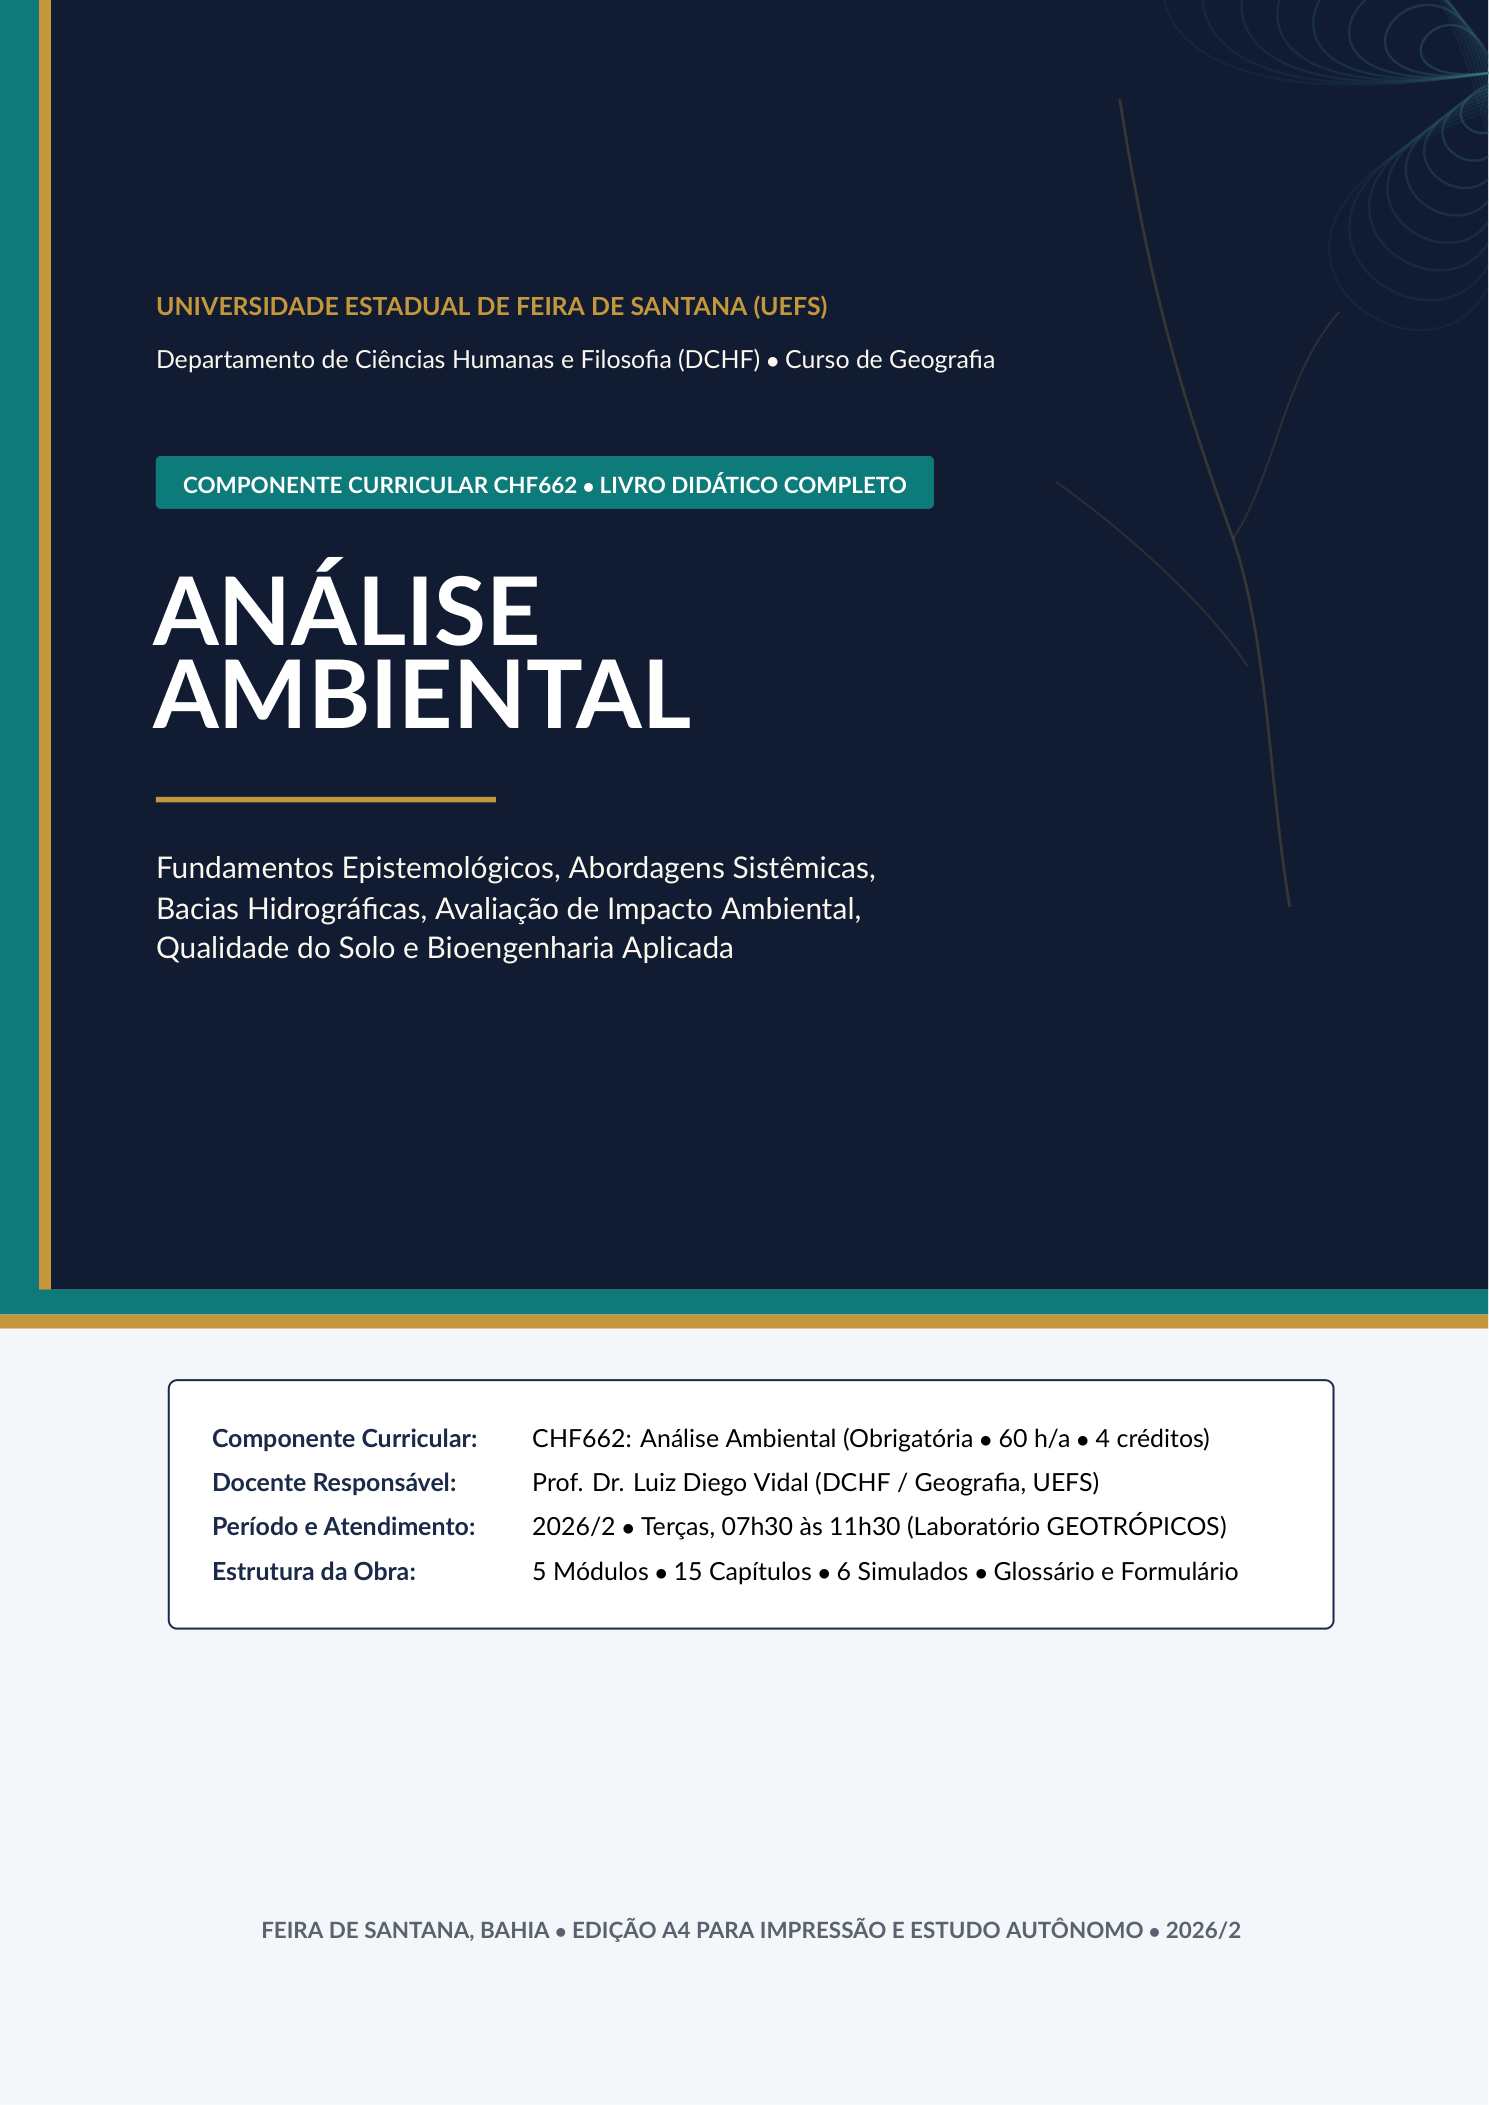
\includegraphics[keepaspectratio,alt={Capa da apostila de Análise Ambiental da UEFS}]{img/capa_analise_ambiental.png}}

}

\caption{Apostila de Análise Ambiental, componente CHF662, Geografia da
Universidade Estadual de Feira de Santana.}

\end{figure}%

\href{APOSTILA_ANALISE_AMBIENTAL_CHF662_UEFS.pdf}{Baixar a apostila em
PDF}

\section*{A análise ambiental como leitura integrada do
território}\label{a-anuxe1lise-ambiental-como-leitura-integrada-do-territuxf3rio}
\addcontentsline{toc}{section}{A análise ambiental como leitura
integrada do território}

\markright{A análise ambiental como leitura integrada do território}

A análise ambiental investiga como processos físicos, organismos, usos
da terra e relações sociais participam da transformação do território.
Seu trabalho envolve reconhecer problemas, formular explicações,
selecionar dados e justificar decisões. A observação de um processo
erosivo exige relacionar chuva, materiais do terreno, circulação da água
e formas de ocupação, acompanhando suas consequências sobre ecossistemas
e populações.

Esta apostila acompanha o componente \textbf{CHF662, Análise Ambiental},
do Curso de Geografia da Universidade Estadual de Feira de Santana,
vinculado ao Departamento de Ciências Humanas e Filosofia. O percurso
reúne fundamentos epistemológicos, conceitos operacionais e métodos
aplicados a bacias hidrográficas, vertentes, solos e áreas degradadas. O
Semiárido baiano e os usos múltiplos do Rio São Francisco aproximam esse
percurso das situações examinadas em campo.

O objetivo é capacitar o estudante a compreender e aplicar os
fundamentos teórico-metodológicos da análise ambiental, integrando
componentes físico-bióticos e socioespaciais ao diagnóstico, à
interpretação e à proposição de medidas de planejamento, conservação e
recuperação. A formação envolve explicar os mecanismos observados,
conferir números e unidades, reconhecer limites dos métodos e comunicar
os resultados com clareza.

\section*{Organização do
conteúdo}\label{organizauxe7uxe3o-do-conteuxfado}
\addcontentsline{toc}{section}{Organização do conteúdo}

\markright{Organização do conteúdo}

Os cinco módulos compreendem 15 capítulos de conteúdo. Os simulados são
atividades de revisão e mantêm numeração independente dos capítulos. Ao
final, uma avaliação integrada, o formulário técnico, o glossário e as
referências apoiam a consulta e a preparação dos produtos da disciplina.

{\def\LTcaptype{none} % do not increment counter
\begin{longtable}[]{@{}
  >{\raggedright\arraybackslash}p{(\linewidth - 4\tabcolsep) * \real{0.3333}}
  >{\raggedright\arraybackslash}p{(\linewidth - 4\tabcolsep) * \real{0.3333}}
  >{\raggedright\arraybackslash}p{(\linewidth - 4\tabcolsep) * \real{0.3333}}@{}}
\toprule\noalign{}
\begin{minipage}[b]{\linewidth}\raggedright
Módulo
\end{minipage} & \begin{minipage}[b]{\linewidth}\raggedright
Capítulos
\end{minipage} & \begin{minipage}[b]{\linewidth}\raggedright
Relação entre os conteúdos
\end{minipage} \\
\midrule\noalign{}
\endhead
\bottomrule\noalign{}
\endlastfoot
Fundamentos epistemológicos e conceituais & 1 a 4 & Questão ambiental,
relação sociedade-natureza, abordagens geográficas e conceitos que
sustentam o diagnóstico. \\
Avaliação de impacto e análise integrada & 5 e 6 & Construção de
cenários, comparação de alternativas e relações entre componentes e
escalas ambientais. \\
Bacias, vertentes e fragilidade & 7 a 9 & Circulação da água,
organização do relevo e dos solos e interpretação da transformação da
paisagem. \\
Indicadores, solos e erosão & 10 a 12 & Desenho do monitoramento,
avaliação de funções do solo e quantificação da degradação. \\
Bioengenharia, legislação e diagnóstico & 13 a 15 & Seleção de
intervenções, enquadramento e elaboração de um diagnóstico ambiental
aplicado. \\
\end{longtable}
}

A ementa articula a questão ambiental contemporânea às abordagens
sistêmicas e integradoras, ao planejamento territorial e à bacia
hidrográfica como unidade de análise. Inclui avaliação de impacto
ambiental, indicadores de qualidade do solo, morfopedologia,
fragilidade, vulnerabilidade, risco, bioengenharia de água e solo,
legislação e recuperação de áreas degradadas.

\section*{Como desenvolver o estudo}\label{como-desenvolver-o-estudo}
\addcontentsline{toc}{section}{Como desenvolver o estudo}

\markright{Como desenvolver o estudo}

Cada capítulo apresenta dez momentos de aprendizagem. Os objetivos e a
retomada dos conhecimentos necessários situam o tema, enquanto a
fundamentação teórica desenvolve conceitos, mecanismos e condições de
aplicação. Os exemplos resolvidos explicitam dados, unidades, cálculos e
interpretação, permitindo acompanhar como uma pergunta é transformada em
uma resposta técnica.

A discussão dos erros frequentes ajuda a conferir o raciocínio antes da
resolução dos exercícios. As atividades de fixação e as questões
autorais no estilo de exames permitem aplicar o conteúdo em situações
novas. O gabarito comentado deve ser consultado após a tentativa de
resolução, confrontando o método utilizado, o resultado e sua
interpretação. A síntese e a verificação final orientam a revisão das
dificuldades identificadas.

Nos exemplos numéricos, os valores fornecidos para treinamento
representam \textbf{dados didáticos}. Resultados de pesquisas são
identificados por sua fonte e por suas condições de obtenção. A
transferência de um resultado para outra área depende da compatibilidade
entre materiais, escala, clima, método e objetivo de análise.

A rotina sugerida combina leitura prévia, participação nas discussões e
retomada dos exemplos após a aula. O registro das dúvidas deve indicar
onde o raciocínio ficou incompleto, como na escolha de uma variável, na
conversão de unidade ou na interpretação de uma hipótese. Esse registro
ajuda a dirigir a revisão.

\section*{Avaliação da disciplina}\label{avaliauxe7uxe3o-da-disciplina}
\addcontentsline{toc}{section}{Avaliação da disciplina}

\markright{Avaliação da disciplina}

O plano organiza a avaliação por estudos orientados, prova teórica e
trabalho prático. Os simulados apoiam o estudo e a autoavaliação. As
orientações institucionais e as instruções fornecidas em aula definem as
condições das atividades avaliativas.

{\def\LTcaptype{none} % do not increment counter
\begin{longtable}[]{@{}
  >{\raggedright\arraybackslash}p{(\linewidth - 6\tabcolsep) * \real{0.2500}}
  >{\raggedright\arraybackslash}p{(\linewidth - 6\tabcolsep) * \real{0.2500}}
  >{\raggedleft\arraybackslash}p{(\linewidth - 6\tabcolsep) * \real{0.2500}}
  >{\raggedleft\arraybackslash}p{(\linewidth - 6\tabcolsep) * \real{0.2500}}@{}}
\toprule\noalign{}
\begin{minipage}[b]{\linewidth}\raggedright
Instrumento
\end{minipage} & \begin{minipage}[b]{\linewidth}\raggedright
Produto e abrangência
\end{minipage} & \begin{minipage}[b]{\linewidth}\raggedleft
Pontos máximos
\end{minipage} & \begin{minipage}[b]{\linewidth}\raggedleft
Participação
\end{minipage} \\
\midrule\noalign{}
\endhead
\bottomrule\noalign{}
\endlastfoot
Estudos orientados EO1 a EO4 & Quatro atividades individuais associadas
aos textos-base e aos capítulos 2 a 5. Cada atividade vale 0,5 ponto. &
2,0 & 20\% \\
Avaliação teórica individual & Prova predominantemente dissertativa,
abrangendo os capítulos 1 a 9. & 3,0 & 30\% \\
Trabalho prático final & Diagnóstico aplicado, com caracterização,
interpretação, indicadores e proposta de intervenção. & 5,0 & 50\% \\
Total & Soma dos pontos obtidos nos instrumentos. & 10,0 & 100\% \\
\end{longtable}
}

A nota final resulta da soma das pontuações efetivamente obtidas. Os
limites de 0,5 ponto por estudo orientado, 3,0 pontos para a prova e 5,0
pontos para o trabalho evitam a aplicação duplicada de pesos sobre
valores já expressos em pontos.

\section*{Cronograma e articulação com o trabalho
final}\label{cronograma-e-articulauxe7uxe3o-com-o-trabalho-final}
\addcontentsline{toc}{section}{Cronograma e articulação com o trabalho
final}

\markright{Cronograma e articulação com o trabalho final}

O quadro organiza o percurso temático em 16 entradas semanais do plano.
A carga horária do componente é de \textbf{60 horas-aula}. A
distribuição dos encontros, das avaliações e do campo acompanha o
calendário acadêmico e as orientações da disciplina.

{\def\LTcaptype{none} % do not increment counter
\begin{longtable}[]{@{}
  >{\raggedleft\arraybackslash}p{(\linewidth - 4\tabcolsep) * \real{0.3333}}
  >{\raggedright\arraybackslash}p{(\linewidth - 4\tabcolsep) * \real{0.3333}}
  >{\raggedright\arraybackslash}p{(\linewidth - 4\tabcolsep) * \real{0.3333}}@{}}
\toprule\noalign{}
\begin{minipage}[b]{\linewidth}\raggedleft
Semana
\end{minipage} & \begin{minipage}[b]{\linewidth}\raggedright
Tema e leitura
\end{minipage} & \begin{minipage}[b]{\linewidth}\raggedright
Atividade e produto de estudo
\end{minipage} \\
\midrule\noalign{}
\endhead
\bottomrule\noalign{}
\endlastfoot
1 & Capítulo 1, questão ambiental e Geografia. & Reconhecimento dos
problemas e de suas relações territoriais. \\
2 & Capítulo 2, modernidade e sociedade-natureza. & Estudo orientado
EO1. \\
3 & Capítulo 3, abordagens socioambientais e GTP. & Estudo orientado
EO2. \\
4 & Capítulo 4, conceitos e risco. & Estudo orientado EO3 e revisão do
módulo 1. \\
5 & Capítulo 5, avaliação de impacto ambiental. & Estudo orientado
EO4. \\
6 & Capítulo 6, análise integrada e escalas. & Revisão do módulo 2 e
definição preliminar da área do trabalho. \\
7 & Capítulo 7, bacias e morfometria. & Delimitação da bacia e
conferência das medidas e unidades. \\
8 & Capítulo 8, morfopedologia e vertentes. & Relações entre relevo,
solos e circulação da água. \\
9 & Capítulo 9, geossistemas e fragilidade. & Construção e interpretação
de sínteses ambientais. \\
10 & Revisão dos capítulos 1 a 9. & Avaliação teórica e simulado
preparatório do módulo 3. \\
11 & Capítulo 10, indicadores e campo. & Observação do eixo energético e
matriz de monitoramento. \\
12 & Capítulo 11, qualidade do solo. & Seleção de indicadores e
comparação com referência. \\
13 & Capítulo 12, degradação e erosão. & Quantificação, limites dos
modelos e revisão do módulo 4. \\
14 & Capítulo 13, bioengenharia. & Seleção de intervenções e critérios
de acompanhamento. \\
15 & Capítulo 14, legislação e PRAD. & Enquadramento e metas de
recuperação. \\
16 & Capítulo 15, diagnóstico aplicado. & Integração, apresentação do
trabalho e revisão do módulo 5. \\
\end{longtable}
}

O trabalho final pode examinar uma microbacia, uma encosta, uma margem
ou outra unidade justificada pela pergunta de análise. Sua elaboração
deve avançar com o estudo, mantendo os dados organizados por fonte,
data, unidade e método. As conclusões devem distinguir observação,
hipótese e previsão, relacionando cada proposta ao processo que se
pretende modificar.

\section*{Fontes, figuras e condições de
uso}\label{fontes-figuras-e-condiuxe7uxf5es-de-uso}
\addcontentsline{toc}{section}{Fontes, figuras e condições de uso}

\markright{Fontes, figuras e condições de uso}

As imagens utilizam referências da disciplina, o acervo disponibilizado
pelo docente e figuras de estudos identificados nas legendas. Imagens
externas mantêm créditos e licenças específicas. As versões submetidas
de estudos são identificadas como manuscritos.

O texto é disponibilizado sob licença
\href{https://creativecommons.org/licenses/by-nc-sa/4.0/}{Creative
Commons Atribuição-NãoComercial-CompartilhaIgual 4.0}. As licenças
próprias das imagens estão indicadas junto às reproduções e no registro
de fontes ao final do livro.

\part{Módulo 1. Fundamentos epistemológicos e conceituais}

\chapter{A Questão Ambiental Contemporânea e o Papel da
Geografia}\label{a-questuxe3o-ambiental-contemporuxe2nea-e-o-papel-da-geografia}

A questão ambiental envolve as condições de reprodução da vida, a
transformação dos sistemas naturais e a distribuição social de
benefícios e danos. Uma análise geográfica começa pela identificação dos
processos que conectam esses planos. A perda de solo em uma encosta, por
exemplo, depende da chuva e das propriedades do terreno, enquanto a
exposição da superfície também resulta de decisões sobre produção,
infraestrutura e acesso à terra.

\section{Etapa 1 - Objetivos de
aprendizagem}\label{etapa-1---objetivos-de-aprendizagem}

A aprendizagem se concentra na construção de explicações que articulem
processos ambientais e organização do território. Ao interpretar uma
situação de degradação, o estudante deve reconhecer o problema,
identificar os grupos envolvidos e justificar quais observações permitem
sustentar a explicação proposta.

\section{Etapa 2 - Conhecimentos
necessários}\label{etapa-2---conhecimentos-necessuxe1rios}

A leitura exige familiaridade com o ciclo da água, as funções da
cobertura vegetal e o conceito de espaço geográfico. A chuva fornece
água e energia ao sistema, enquanto o uso da terra modifica a
infiltração e o percurso do escoamento. A escala de observação define
quais dessas relações podem ser reconhecidas nos dados.

\section{Etapa 3 - Fundamentação
teórica}\label{etapa-3---fundamentauxe7uxe3o-teuxf3rica}

\subsection{Vocabulário Técnico e Conceitos-Chave do
Capítulo}\label{vocabuluxe1rio-tuxe9cnico-e-conceitos-chave-do-capuxedtulo}

{\def\LTcaptype{none} % do not increment counter
\begin{longtable}[]{@{}
  >{\raggedright\arraybackslash}p{(\linewidth - 2\tabcolsep) * \real{0.5000}}
  >{\raggedright\arraybackslash}p{(\linewidth - 2\tabcolsep) * \real{0.5000}}@{}}
\toprule\noalign{}
\begin{minipage}[b]{\linewidth}\raggedright
\textbf{Termo / Conceito}
\end{minipage} & \begin{minipage}[b]{\linewidth}\raggedright
\textbf{Definição Operacional em Análise Ambiental}
\end{minipage} \\
\midrule\noalign{}
\endhead
\bottomrule\noalign{}
\endlastfoot
\textbf{Questão ambiental} & Conjunto de tensões ecológicas, econômicas,
políticas e culturais derivadas do modo como as sociedades
contemporâneas se apropriam da natureza e distribuem benefícios e danos
ambientais. \\
\textbf{Crise civilizatória} & Crise estrutural do modelo
moderno-industrial de produção, consumo e organização do conhecimento,
cujos limites ultrapassam falhas pontuais de engenharia ou gestão (Leff,
2001). \\
\textbf{Racionalidade econômica} & Lógica dominante voltada à
maximização do crescimento, do lucro e da eficiência produtiva de curto
prazo, frequentemente externalizando custos ecológicos e sociais. \\
\textbf{Racionalidade ambiental} & Racionalidade alternativa orientada
pela articulação entre produtividade ecológica, equidade social,
diversidade cultural e gestão democrática do território (Leff, 2001). \\
\textbf{Saber ambiental} & Campo emergente de conhecimentos que
questiona a fragmentação científica tradicional e integra saberes
disciplinares e locais em torno da complexidade socioambiental (Leff,
2001). \\
\textbf{Interdisciplinaridade} & Rearticulação conceitual e metodológica
entre diferentes áreas do conhecimento para responder a problemas
complexos, indo além da mera soma de relatórios isolados. \\
\textbf{Desenvolvimento sustentável} & Formulação institucional
disseminada a partir do final do século XX que busca compatibilizar
crescimento econômico, equidade social e conservação ambiental,
frequentemente objeto de disputa política e crítica conceitual. \\
\textbf{Sustentabilidade} & Condição socioecológica de manutenção dos
processos vitais, da integridade dos ecossistemas e da reprodução digna
das coletividades humanas no longo prazo (Porto-Gonçalves, 2006). \\
\textbf{Planejamento ambiental} & Processo técnico, político e contínuo
de diagnóstico, prognóstico, ordenamento de usos e definição de
diretrizes voltadas à conservação, mitigação de impactos e recuperação
de áreas degradadas. \\
\end{longtable}
}

\subsection{A Questão Ambiental Contemporânea, Crise Civilizatória e de
Racionalidade}\label{a-questuxe3o-ambiental-contemporuxe2nea-crise-civilizatuxf3ria-e-de-racionalidade}

Na linguagem cotidiana e em parte da mídia, a expressão ``problema
ambiental'' costuma aparecer reduzida a episódios visíveis e pontuais,
um vazamento de óleo, o acúmulo de resíduos em um riacho urbano ou um
incêndio florestal em determinado município. Embora esses eventos sejam
graves e exijam resposta técnica imediata, reduzi-los a falhas isoladas
impede a compreensão de suas causas estruturais.

A partir da segunda metade do século XX, especialmente após a aceleração
industrial do pós-guerra, a intensificação da urbanização e a expansão
globalizada das fronteiras agropecuárias e extrativistas, tornou-se
evidente que os danos aos ecossistemas não eram acidentes marginais, mas
consequências sistemáticas do próprio modelo de desenvolvimento adotado.
É nesse horizonte que se consolida a \textbf{questão ambiental
contemporânea}, um campo de debates científicos, políticos e
territoriais que põe em xeque a forma como a sociedade moderna produz,
consome, ocupa o espaço e constrói conhecimento.

Em \emph{Epistemologia ambiental} (2001, cap. 2,
\emph{Interdisciplinaridade, ambiente e desenvolvimento sustentável}),
Enrique Leff demonstra que a crise ambiental não é apenas uma crise
ecológica (isto é, uma perturbação restrita aos ciclos biogeoquímicos),
mas uma \textbf{crise civilizatória e de racionalidade}. Segundo o
autor, a modernidade consolidou uma \textbf{racionalidade econômica e
instrumental} que trata a natureza como estoque inesgotável de
matérias-primas e como depósito passivo de rejeitos. Nessa lógica, os
danos gerados sobre o solo, a água, a biodiversidade e a saúde humana
são tratados como ``externalidades'', ficando de fora do cálculo
econômico tradicional.

Ao mesmo tempo, essa racionalidade econômica apoiou-se na
\textbf{fragmentação disciplinar do conhecimento científico}. Cada
ciência especializou-se em recortar um fragmento da realidade, a
agronomia focou a produtividade da cultura, a engenharia civil
concentrou-se na resistência de estruturas, a economia modelou fluxos
monetários e a sociologia examinou instituições humanas, muitas vezes
sem diálogo efetivo entre si. Diante de fenômenos complexos como a
desertificação, a degradação de bacias hidrográficas ou as mudanças
climáticas, essa divisão estanque mostra-se insuficiente.

\subsection{Saber Ambiental e Interdisciplinaridade em Enrique Leff
(2001)}\label{saber-ambiental-e-interdisciplinaridade-em-enrique-leff-2001}

Para Leff (2001), superar a crise ambiental exige construir uma
\textbf{racionalidade ambiental} sustentada por um \textbf{saber
ambiental}. Esse saber não substitui o rigor de cada ciência, mas
transforma internamente as disciplinas ao confrontá-las com os limites
ecológicos e com a dimensão cultural e política do território. A
\textbf{interdisciplinaridade ambiental}, portanto, não consiste em
reunir especialistas para escrever capítulos separados em um mesmo
relatório; trata-se de construir perguntas comuns, categorias
integradoras e métodos articulados capazes de apreender o ambiente como
totalidade complexa.

A organização do conhecimento influencia a forma de reconhecer e
enfrentar a degradação (Figura~\ref{fig-racionalidades}). A abordagem
integrada relaciona componentes e escalas, permitindo que a proposta de
intervenção responda aos processos e às consequências identificados.

\begin{figure}[H]

\centering{

\pandocbounded{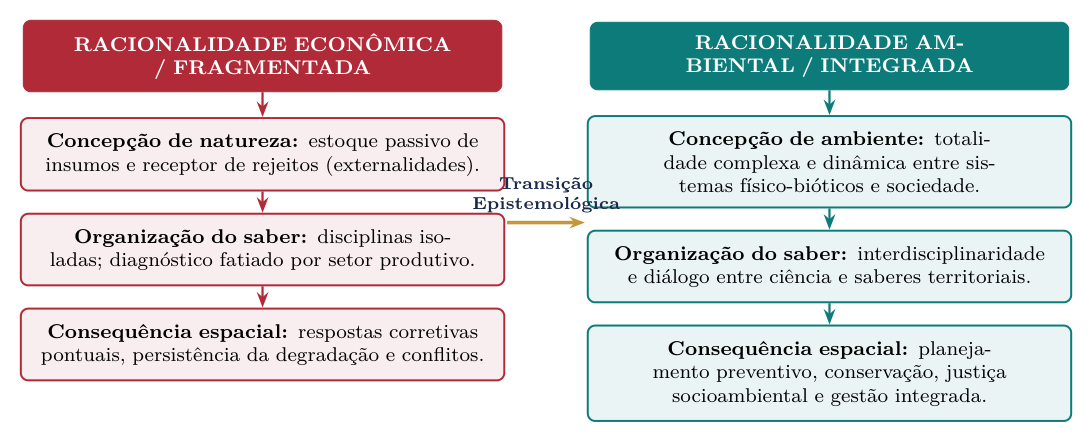
\includegraphics[keepaspectratio,alt={Duas sequências com concepção de natureza, organização do conhecimento e consequências territoriais}]{capitulos/../img/esquema_racionalidades.png}}

}

\caption{\label{fig-racionalidades}Comparação entre racionalidade
econômica fragmentada e racionalidade ambiental integrada. Diagrama do
material da disciplina, recomposto a partir da fonte vetorial original,
com base em Leff (2001).}

\end{figure}%

Na prática da Análise Ambiental, é frequente confundir
\emph{multidisciplinaridade} com \emph{interdisciplinaridade}. A
Tabela~\hyperref[tbl-disciplinas_cap1]{disciplinas cap1} apresenta os
critérios operacionais que distinguem essas formas de organização do
trabalho técnico e científico.

\protect\phantomsection\label{tbl-disciplinas_cap1}{}

{\def\LTcaptype{none} % do not increment counter
\begin{longtable}[]{@{}
  >{\raggedright\arraybackslash}p{(\linewidth - 6\tabcolsep) * \real{0.2500}}
  >{\raggedright\arraybackslash}p{(\linewidth - 6\tabcolsep) * \real{0.2500}}
  >{\raggedright\arraybackslash}p{(\linewidth - 6\tabcolsep) * \real{0.2500}}
  >{\raggedright\arraybackslash}p{(\linewidth - 6\tabcolsep) * \real{0.2500}}@{}}
\toprule\noalign{}
\begin{minipage}[b]{\linewidth}\raggedright
\textbf{Dimensão}
\end{minipage} & \begin{minipage}[b]{\linewidth}\raggedright
\textbf{Disciplinaridade Isolada}
\end{minipage} & \begin{minipage}[b]{\linewidth}\raggedright
\textbf{Multidisciplinaridade}
\end{minipage} & \begin{minipage}[b]{\linewidth}\raggedright
\textbf{Interdisciplinaridade Ambiental}
\end{minipage} \\
\midrule\noalign{}
\endhead
\bottomrule\noalign{}
\endlastfoot
\textbf{Formulação do problema} & Definida apenas nos limites de uma
especialidade. & Cada área analisa o mesmo local sob sua própria ótica,
em paralelo. & Problema construído conjuntamente, reconhecendo
interações físico-bióticas e sociais. \\
\textbf{Relação entre métodos} & Método único e fechado. & Justaposição
de laudos e mapas que raramente dialogam entre si. & Integração
metodológica (por exemplo, cruzamento entre uso da terra, erosão e
vulnerabilidade social). \\
\textbf{Produto típico} & Parecer setorial (por exemplo, apenas análise
química da água). & Relatório ``colcha de retalhos'' com anexos
desconectados. & Diagnóstico ambiental integrado com síntese causal e
diretrizes coerentes de gestão. \\
\textbf{Limite ou ganho} & Alta profundidade local, mas cegueira para
causas sistêmicas. & Amplia o volume de dados, porém sem explicar as
interações. & Permite intervir sobre as causas da degradação, e não
apenas sobre seus sintomas. \\
\end{longtable}
}

\textbf{Tabela 1.1,} Comparação entre abordagens disciplinar,
multidisciplinar e interdisciplinar na Análise Ambiental (elaborada com
base em Leff, 2001; Tauk-Tornisielo,
1996).\protect\phantomsection\label{tab:disciplinas_cap1}{}

\subsection{Degradação dos Solos, Escassez Hídrica e Mudanças no Uso da
Terra}\label{degradauxe7uxe3o-dos-solos-escassez-huxeddrica-e-mudanuxe7as-no-uso-da-terra}

Para que o debate epistemológico não permaneça abstrato, é essencial
observar como a crise ambiental se materializa na superfície terrestre.
No Brasil, e de maneira particularmente aguda no Nordeste e no Semiárido
Baiano, três processos interligados concentram grande parte dos desafios
da Análise Ambiental, a \textbf{degradação dos solos}, a
\textbf{escassez hídrica} e as \textbf{mudanças no uso e cobertura da
terra}.

\subsubsection{Mudanças no Uso da Terra como Vetor
Desencadeador}\label{mudanuxe7as-no-uso-da-terra-como-vetor-desencadeador}

A cobertura vegetal nativa exerce funções hidrogeomorfológicas
decisivas, intercepta a precipitação, dissipa a energia cinética das
gotas de chuva, fornece matéria orgânica que estabiliza os agregados do
solo e mantém canais radiculares que ampliam a infiltração da água.
Quando áreas de Caatinga, Cerrado ou Mata Atlântica são suprimidas sem
planejamento conservacionista para dar lugar a pastagens extensivas de
alta lotação, monocultivos mecanizados, abertura desordenada de estradas
rurais, mineração ou expansão urbana em encostas e fundos de vale,
altera-se abruptamente o balanço entre infiltração e escoamento
superficial.

Na Bahia, esse processo assume expressões regionais distintas,

\textbf{Semiárido Baiano (domínio da Caatinga).} Combina supressão da
vegetação lenhosa para extração de lenha e carvão, sobrepastoreio
caprino/bovino em áreas já frágeis, manejo inadequado de lavouras de
sequeiro e implantação de grandes infraestruturas (estradas, linhas de
transmissão, parques energéticos) que expõem solos rasos e pedregosos
(como Neossolos Litólicos e Planossolos) a chuvas concentradas em poucos
meses do ano. \textbf{Oeste Baiano (domínio do Cerrado).} Caracteriza-se
pela rápida conversão de vegetação nativa em agricultura mecanizada de
larga escala, intensificando a demanda por águas superficiais e
subterrâneas e modificando a dinâmica de recarga em chapadões arenosos.

\textbf{Faixa litorânea, Recôncavo e centros urbanos regionais (como o
entorno de Feira de Santana).} Evidencia impermeabilização acelerada do
solo, supressão de áreas de preservação permanente (APPs) de nascentes,
lagoas e riachos, lançamento de efluentes sem tratamento adequado e
expansão de loteamentos sobre áreas sujeitas a alagamentos ou
instabilidade de vertentes.

\subsubsection{Degradação dos Solos e Processos
Erosivos}\label{degradauxe7uxe3o-dos-solos-e-processos-erosivos}

O solo não é um substrato inerte sobre o qual se constroem edificações
ou se aplicam fertilizantes; trata-se de um corpo natural
tridimensional, dinâmico e vivo, cuja formação (pedogênese) demanda
séculos ou milênios. A degradação edáfica manifesta-se pela perda
progressiva de suas funções físicas, químicas e biológicas, redução do
teor de matéria orgânica, quebra dos agregados, selamento superficial,
compactação pelo pisoteio animal ou tráfego de máquinas, salinização em
perímetros irrigados mal drenados e remoção acelerada de partículas pela
erosão hídrica e eólica.

Quando a taxa de remoção de solo supera amplamente a taxa natural de
formação, a erosão evolui da forma \emph{laminar} (lavagem difusa da
camada superficial mais fértil) para a forma \emph{linear} (sulcos,
ravinas e voçorocas). Os sedimentos mobilizados das encostas não
desaparecem, são transportados pela rede de drenagem e depositados em
calhas fluviais, barreiros, cisternas rurais e açudes, reduzindo sua
capacidade de armazenamento de água.

\subsubsection{Escassez Hídrica, Condição Climática versus Produção
Socioambiental}\label{escassez-huxeddrica-condiuxe7uxe3o-climuxe1tica-versus-produuxe7uxe3o-socioambiental}

Um dos equívocos mais persistentes sobre o Nordeste brasileiro é
explicar a escassez hídrica exclusivamente pela baixa média
pluviométrica. O clima semiárido apresenta, de fato, chuvas concentradas
no tempo, elevada variabilidade interanual e altas taxas de
evapotranspiração potencial, características naturais que definem a
\textbf{semiaridez}. Contudo, a \textbf{escassez hídrica vivenciada pela
população} é resultado direto da interação entre essa dinâmica climática
e fatores socioespaciais, desmatamento das cabeceiras e matas ciliares,
compactação do solo (que impede a recarga do lençol freático),
assoreamento de reservatórios, contaminação de mananciais e distribuição
desigual da infraestrutura de captação e acesso à água.

\subsection{Cadeia de Retroalimentação Solo-Água-Uso da
Terra}\label{01-questao-ambiental-cadeia-de-retroalimentauxe7uxe3o-solouxe1guauso-da-terra}

Degradação dos solos, escassez hídrica e mudança no uso da terra não
ocorrem como listas paralelas de problemas, elas formam um circuito
retroalimentado. A supressão vegetal reduz a infiltração e intensifica o
escoamento superficial; o escoamento acelerado remove o solo fértil e
assoreia os corpos d'água; a perda de fertilidade e de disponibilidade
hídrica pressiona os produtores a expandir o desmatamento sobre novas
áreas frágeis, ampliando a vulnerabilidade socioambiental.

A conexão entre uso da terra, perda de solo e disponibilidade hídrica
pode ampliar a pressão sobre novas áreas
(Figura~\ref{fig-solo-agua-uso}). A análise deve localizar os pontos de
entrada de uma medida de conservação e explicar como ela modifica esse
circuito.

\begin{figure}[H]

\centering{

\pandocbounded{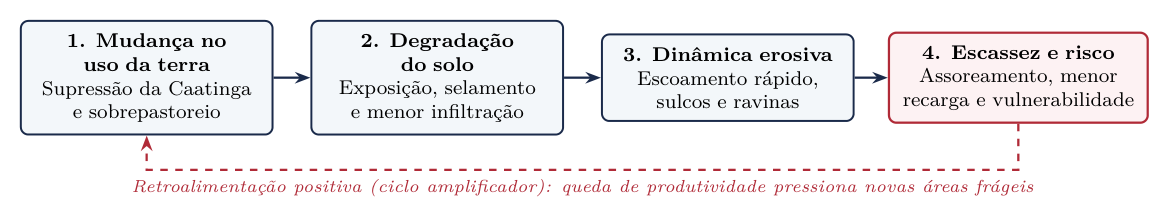
\includegraphics[keepaspectratio,alt={Sequência de mudanças no uso da terra, degradação do solo, erosão e escassez, com uma ligação de retroalimentação}]{capitulos/../img/esquema_solo_agua_uso.png}}

}

\caption{\label{fig-solo-agua-uso}Relações entre uso da terra,
degradação do solo, erosão e escassez hídrica. Diagrama do material da
disciplina, recomposto a partir da fonte vetorial original.}

\end{figure}%

\subsection{O Debate Crítico, Desenvolvimento Sustentável versus
Sustentabilidade}\label{o-debate-cruxedtico-desenvolvimento-sustentuxe1vel-versus-sustentabilidade}

A partir da publicação do Relatório \emph{Nosso Futuro Comum} (Relatório
Brundtland, 1987) e da Conferência das Nações Unidas sobre Meio Ambiente
e Desenvolvimento (Rio-92), a expressão \textbf{desenvolvimento
sustentável} ganhou enorme visibilidade internacional, sendo definida
como aquele capaz de atender às necessidades do presente sem comprometer
a capacidade das gerações futuras de atenderem às suas próprias
necessidades.

À primeira vista, a formulação parece consensual e inquestionável.
Entretanto, autores como Carlos Walter Porto-Gonçalves (\emph{Os
(des)caminhos do meio ambiente}, 2006) e Enrique Leff (2001) demonstram
que o conceito abriga contradições profundas. Porto-Gonçalves chama
atenção para a estrutura política da expressão, ao acoplar o adjetivo
``sustentável'' ao substantivo ``desenvolvimento'', o discurso
institucional dominante preserva intacto o projeto desenvolvimentista
baseado na expansão contínua da produção de mercadorias, no consumo
crescente de energia e na subordinação de territórios periféricos ao
mercado mundial.

Sob essa perspectiva crítica, a noção de desenvolvimento sustentável
muitas vezes opera como mecanismo de \emph{recodificação econômica da
natureza}, a floresta, a água e o clima passam a ser valorados apenas
como ``capital natural'' ou ``serviços mercantilizáveis'', sem
questionar quem detém o controle dos territórios, quem se beneficia dos
ganhos econômicos e quem arca com a poluição, o deslocamento compulsório
e a degradação do solo.

Em contraposição, o debate sobre \textbf{sustentabilidade} (ou
sustentabilidade socioambiental) propõe deslocar o foco do crescimento
econômico ilimitado para a manutenção da integridade ecológica, da
diversidade cultural e da equidade territorial. A sustentabilidade,
nesse sentido, não é um selo de marketing empresarial nem uma meta
técnica universalmente imposta de cima para baixo, mas um projeto
histórico e geográfico que reconhece os limites biofísicos dos
ecossistemas e valoriza modos locais de convivência com o ambiente, como
as estratégias de convivência com o Semiárido baseadas em conservação de
solo, captação descentralizada de água de chuva e manejo sustentável da
Caatinga.

{\def\LTcaptype{none} % do not increment counter
\begin{longtable}[]{@{}
  >{\raggedright\arraybackslash}p{(\linewidth - 4\tabcolsep) * \real{0.3333}}
  >{\raggedright\arraybackslash}p{(\linewidth - 4\tabcolsep) * \real{0.3333}}
  >{\raggedright\arraybackslash}p{(\linewidth - 4\tabcolsep) * \real{0.3333}}@{}}
\toprule\noalign{}
\begin{minipage}[b]{\linewidth}\raggedright
\textbf{Critério de Análise}
\end{minipage} & \begin{minipage}[b]{\linewidth}\raggedright
\textbf{Discurso Hegemônico de Desenvolvimento Sustentável}
\end{minipage} & \begin{minipage}[b]{\linewidth}\raggedright
\textbf{Perspectiva Crítica de Sustentabilidade Socioambiental}
\end{minipage} \\
\midrule\noalign{}
\endhead
\bottomrule\noalign{}
\endlastfoot
\textbf{Eixo central} & Conciliar crescimento econômico contínuo com
eficiência tecnológica e controle de impactos. & Garantir integridade
dos sistemas ecológicos, justiça socioambiental e reprodução digna da
vida. \\
\textbf{Leitura da natureza} & Capital natural, estoque de recursos
mensuráveis pelo mercado e ativos compensáveis. & Patrimônio
socioecológico complexo, dotado de limites biofísicos e significados
culturais plurais. \\
\textbf{Papel da técnica} & Solução principal para a crise
(ecoeficiência, substituição de insumos, mercado verde). & Ferramenta
necessária, mas subordinada a critérios éticos, ecológicos e
democráticos de decisão. \\
\textbf{Relação com o território} & Tende a homogeneizar modelos
produtivos e minimizar conflitos distributivos. & Reconhece conflitos
territoriais, desigualdades de poder e diversidade de saberes locais. \\
\textbf{Referência-base} & Crítica formulada em Leff (2001, cap. 2) e
Porto-Gonçalves (2006). & Proposta articulada em Leff (2001),
Porto-Gonçalves (2006) e na Geografia Socioambiental. \\
\end{longtable}
}

\textbf{Tabela 1.2,} Síntese comparativa entre o discurso convencional
de desenvolvimento sustentável e a perspectiva crítica de
sustentabilidade.

\subsection{Planejamento Ambiental e o Papel Integrador da
Geografia}\label{planejamento-ambiental-e-o-papel-integrador-da-geografia}

Diante de uma crise simultaneamente ecológica, econômica e territorial,
o \textbf{planejamento ambiental} apresenta-se como instrumento
fundamental de mediação entre a dinâmica da natureza e as demandas da
sociedade. Planejar ambientalmente significa ir além de ações
emergenciais pós-desastre, envolve levantar evidências empíricas sobre o
meio físico, biótico e socioespacial (diagnóstico), projetar tendências
de degradação ou recuperação sob diferentes cenários de uso da terra
(prognóstico), estabelecer diretrizes de zoneamento, conservação e
restauração (ordenamento) e acompanhar continuamente os resultados por
meio de indicadores auditáveis (monitoramento).

É precisamente nesse terreno que a \textbf{Geografia} desempenha um
papel integrador insubstituível frente à fragmentação disciplinar,

\textbf{Articulação físico-biótico-socioespacial.} A formação geográfica
capacita o profissional a ler simultaneamente o relevo, os solos, a rede
de drenagem e a cobertura vegetal juntamente com a estrutura fundiária,
a urbanização, as redes de infraestrutura e os conflitos territoriais.
\textbf{Domínio da espacialidade e da cartografia.} Problemas ambientais
nunca são abstratos; eles têm localização, extensão, conectividade e
padrões espaciais que podem ser mapeados, modelados e cruzados em
Sistemas de Informação Geográfica (SIG) e trabalhos de campo.

\textbf{Leitura multiescalar.} O(a) geógrafo(a) conecta processos que
ocorrem na escala da parcela de solo ou da vertente (erosão em sulcos)
com a escala da bacia hidrográfica (assoreamento de mananciais), da
região (políticas para o Semiárido) e das redes econômicas globais
(demanda por energia e commodities). \textbf{Mediação interdisciplinar.}
Por transitar entre as ciências da Terra e as ciências humanas, a
Geografia atua como ponte entre engenheiros, biólogos, agrônomos,
gestores públicos e comunidades locais na construção de diagnósticos
ambientais coerentes.

\subsection{Conexão Direta com os Próximos Módulos e o Trabalho Prático
Final}\label{conexuxe3o-direta-com-os-pruxf3ximos-muxf3dulos-e-o-trabalho-pruxe1tico-final}

Tudo o que você estudará nos próximos capítulos de CHF662 desdobra os
fundamentos apresentados aqui, no Módulo 2, a Avaliação de Impacto
Ambiental (AIA) e a análise integrada; no Módulo 3, a bacia
hidrográfica, a morfopedologia, os geossistemas e a fragilidade
ambiental; no Módulo 4, os indicadores ambientais e de qualidade do solo
(incluindo a viagem de campo no Semiárido Baiano); e no Módulo 5, a
bioengenharia de água e solo, a legislação e o Diagnóstico Ambiental
Aplicado (50\% da nota final). Manter desde o Capítulo 1 o hábito de
integrar processos naturais e decisões sociais evitará diagnósticos
fragmentados na Prova Teórica e no Trabalho Final.

\subsection{Da observação do dano à explicação
geográfica}\label{da-observauxe7uxe3o-do-dano-uxe0-explicauxe7uxe3o-geogruxe1fica}

Uma margem assoreada constitui um ponto de partida para a investigação.
O sedimento pode ter sido produzido em lavouras, estradas ou canais
erosivos situados a montante. A ligação entre a fonte e o local de
deposição depende do caminho percorrido pela água e das oportunidades de
retenção ao longo da bacia. Identificar essa ligação permite explicar
por que uma intervenção localizada na margem pode produzir efeito
limitado enquanto as fontes continuam ativas.

A interpretação ganha consistência quando explicita a sequência
temporal. Fotografias antigas, relatos de moradores e mapas de cobertura
da terra ajudam a verificar se a abertura de acessos antecedeu o
aparecimento de incisões. A coincidência temporal orienta uma hipótese,
cuja avaliação depende da distribuição espacial dos processos, das
condições de chuva e da comparação com setores semelhantes.

O diagnóstico também precisa reconhecer quem utiliza a água e quem
suporta a redução de sua qualidade. A mesma alteração pode afetar
captação doméstica, irrigação e manutenção de habitats por caminhos
distintos. A proposta de gestão deve relacionar cada medida ao processo
que pretende modificar e ao grupo que depende do resultado. Essa
articulação entre mecanismo físico e consequência social dá conteúdo
operacional à abordagem socioambiental.

\section{Etapa 4 - Exemplos
resolvidos}\label{etapa-4---exemplos-resolvidos}

\emph{Nota metodológica,} Os cenários numéricos e localidades
estilizadas abaixo são \textbf{cenários didáticos ilustrativos},
construídos exclusivamente para treinar a aplicação rigorosa dos
referenciais teóricos de Leff (2001) e Porto-Gonçalves (2006) a
situações concretas da prática geográfica.

\subsection{Exemplo 1.1, Básico. Fragmentação Disciplinar em Projeto de
Contenção de
Erosão}\label{exemplo-1.1-buxe1sico.-fragmentauxe7uxe3o-disciplinar-em-projeto-de-contenuxe7uxe3o-de-erosuxe3o}

\textbf{Situação analisada.} Em um município fictício do Semiárido
Baiano \emph{(cenário didático ilustrativo)}, uma prefeitura contratou
uma empresa para conter o assoreamento de um açude comunitário. A equipe
técnica elaborou apenas um projeto de dragagem mecânica do reservatório
e construção de um muro de concreto próximo ao sangradouro, sem avaliar
o uso do solo nas cabeceiras da microbacia nem ouvir os agricultores que
utilizam a água. Dois anos após a obra, o açude voltou a apresentar
acúmulo intenso de sedimentos.

\textbf{Dados disponíveis.} Intervenção exclusivamente
estrutural/corretiva (dragagem e muro de concreto); ausência de
diagnóstico da cobertura vegetal e dos solos nas vertentes a montante;
ausência de participação dos usuários locais; retorno do assoreamento em
2 anos.

\textbf{Problema a resolver.} Diagnosticar a falha epistemológica e
metodológica do projeto à luz de Enrique Leff (2001) e indicar como uma
abordagem interdisciplinar geográfica reestruturaria a intervenção.

\textbf{Fundamento da análise.} Análise epistemológica baseada nos
conceitos de \emph{racionalidade econômica/instrumental},
\emph{fragmentação disciplinar}, \emph{saber ambiental} e
\emph{interdisciplinaridade} (Leff, 2001, cap. 2).

\textbf{Desenvolvimento.}

\textbf{Identificação do sintoma versus causa.} A dragagem atuou apenas
sobre o sintoma final (sedimento acumulado no açude), ignorando a causa
geradora nas vertentes a montante (solo exposto, erosão laminar e
linear, retirada da vegetação ripária). \textbf{Diagnóstico
epistemológico (Leff, 2001).} O projeto reproduziu a \emph{fragmentação
disciplinar} e a \emph{racionalidade instrumental}, tratando um problema
socioambiental complexo como mera questão pontual de engenharia civil.
\textbf{Reestruturação interdisciplinar.} Uma equipe coordenada sob
perspectiva geográfica integrada deveria, (a) delimitar a microbacia de
contribuição do açude; (b) mapear áreas de solo exposto, sobrepastoreio
e focos erosivos nas cabeceiras; (c) dialogar com os agricultores para
identificar pressões de uso da terra e saberes locais de manejo; e (d)
combinar medidas conservacionistas na vertente (recomposição vegetal,
retenção de enxurrada, manejo do pastoreio) com ações de manutenção do
reservatório.

\textbf{Interpretação do resultado.} O fracasso recorrente do projeto
decorre da fragmentação disciplinar e da racionalidade instrumental, que
trataram o assoreamento como falha pontual dissociada da dinâmica da
microbacia e do uso social da terra. A solução exige abordagem
interdisciplinar e planejamento integrado a montante e junto à
comunidade.

\textbf{Condições de validade.} A análise é ambientalmente coerente,
dragar um açude sem reduzir a produção de sedimentos nas encostas apenas
reinicia o ciclo de assoreamento a cada estação chuvosa, desperdiçando
recursos públicos e mantendo a vulnerabilidade hídrica.

\subsection{Exemplo 1.2, Básico. Diferenciando Semiaridez Climática de
Escassez Hídrica
Socioambiental}\label{exemplo-1.2-buxe1sico.-diferenciando-semiaridez-climuxe1tica-de-escassez-huxeddrica-socioambiental}

\textbf{Situação analisada.} Duas microbacias rurais vizinhas no
Semiárido Baiano \emph{(cenário didático ilustrativo)} registram
exatamente a mesma precipitação média anual de \(580\text{ mm}\),
concentrada entre novembro e março, sobre substrato geológico e relevo
semelhantes. Na Microbacia A, \(65\%\) da área mantém cobertura de
Caatinga manejada, faixas de mata ciliar conservadas e práticas de
retenção de água no solo; suas cacimbas permanecem com água na estação
seca. Na Microbacia B, \(78\%\) da área foi convertida em pastagem
degradada com solo compactado e margens desmatadas; os reservatórios
secam rapidamente após as chuvas e o solo apresenta sulcos erosivos.

\textbf{Dados disponíveis.} Precipitação idêntica
(\(580\text{ mm/ano}\)) e substrato semelhante em ambas as microbacias.
Microbacia A, \(65\%\) de vegetação nativa, mata ciliar preservada,
disponibilidade hídrica mantida na estiagem. Microbacia B, \(78\%\) de
pastagem degradada, solo compactado, margens desmatadas, rápida perda de
água e erosão em sulcos.

\textbf{Problema a resolver.} Explicar por que o determinismo climático
não explica a diferença observada entre as duas microbacias e demonstrar
a relação causal entre uso da terra, solo e água.

\textbf{Fundamento da análise.} Análise comparativa controlada (mesmo
clima, diferentes usos da terra) articulando processos
hidrogeomorfológicos básicos e leitura socioambiental da escassez
hídrica.

\textbf{Desenvolvimento.}

\textbf{Controle da variável climática.} Como ambas as microbacias
recebem \(580\text{ mm/ano}\) sob o mesmo regime de chuvas concentradas,
a diferença na disponibilidade de água na estação seca não pode ser
atribuída apenas à falta de chuva. \textbf{Dinâmica na Microbacia A.} A
cobertura vegetal protege a superfície do solo contra o impacto das
gotas de chuva, mantém porosidade elevada e favorece a infiltração,
recarregando o solo e os reservatórios rasos (cacimbas) para o período
seco.

\textbf{Dinâmica na Microbacia B.} A remoção da vegetação e a
compactação reduzem a taxa de infiltração; assim, grande parcela dos
\(580\text{ mm}\) transforma-se rapidamente em escoamento superficial,
gerando sulcos erosivos, arraste de sedimentos e baixa recarga hídrica
subsuperficial. \textbf{Síntese conceitual.} A semiaridez é condição
climática natural comum às duas áreas, mas a escassez hídrica severa na
Microbacia B é agravada pelo modelo de uso e ocupação do solo.

\textbf{Interpretação do resultado.} A diferença decorre do manejo do
uso da terra e das condições do solo, e não apenas do clima, a
degradação vegetal e edáfica na Microbacia B converte a chuva em
escoamento rápido e erosão, reduzindo a infiltração e produzindo
escassez hídrica socioambiental.

\textbf{Condições de validade.} O raciocínio respeita o balanço hídrico
elementar, para uma mesma entrada pluviométrica (\(P = 580\text{ mm}\)),
quanto menor a infiltração em solos degradados, maior o escoamento
superficial imediato e menor a água armazenada disponível durante a
estiagem.

\subsection{Exemplo 1.3, Intermediário. Análise Crítica de um Discurso
de ``Desenvolvimento
Sustentável''}\label{exemplo-1.3-intermediuxe1rio.-anuxe1lise-cruxedtica-de-um-discurso-de-desenvolvimento-sustentuxe1vel}

\textbf{Situação analisada.} Um consórcio agroindustrial divulga um
documento promocional anunciando a implantação de um polo de monocultura
irrigada de exportação em uma bacia hidrográfica de transição
Cerrado-Caatinga \emph{(cenário didático ilustrativo)}. O texto
classifica o empreendimento como exemplo de ``desenvolvimento
sustentável'' porque utilizará pivôs com sensores digitais que
economizam \(15\%\) de água em comparação a sistemas antigos e
compensará a supressão de vegetação nativa mediante a compra de créditos
ambientais em outra região do país.

\textbf{Dados disponíveis.} Alegações do consórcio, ganho de \(15\%\) na
eficiência de irrigação por sensores; compensação ambiental fora da
bacia impactada; expansão de monocultura intensiva com remoção de
vegetação nativa local e aumento da captação hídrica total.

\textbf{Problema a resolver.} Avaliar criticamente o uso do termo
``desenvolvimento sustentável'' nesse documento à luz de Porto-Gonçalves
(2006) e Leff (2001), apontando as limitações socioambientais ocultadas
pela peça promocional.

\textbf{Fundamento da análise.} Análise crítica do discurso ambiental
com base na distinção entre \emph{desenvolvimento sustentável
hegemônico} e \emph{sustentabilidade socioambiental} (Porto-Gonçalves,
2006; Leff, 2001).

\textbf{Desenvolvimento.}

\textbf{Análise do ganho de ecoeficiência (\(15\%\)).} Economizar água
por hectare em relação a técnicas antigas não garante redução do consumo
total de água na bacia se a área irrigada se expandir de forma absoluta.
A técnica melhora a eficiência produtiva sem questionar o limite hídrico
regional. \textbf{Crítica à compensação desterritorializada.} Comprar
créditos ambientais em outra região trata a natureza como mercadoria
intercambiável (lógica da racionalidade econômica criticada por Leff,
2001). Contudo, a biodiversidade, a proteção do solo e a recarga hídrica
perdidas na bacia local não são fisicamente repostas por uma área
conservada a centenas de quilômetros.

\textbf{Ocultamento de dimensões sociais (Porto-Gonçalves, 2006).} O
discurso adota o adjetivo ``sustentável'' para legitimar o modelo
desenvolvimentista, omitindo questões centrais como quem perde acesso à
água a jusante, como se alteram a estrutura fundiária e a segurança
alimentar local e se as comunidades atingidas participaram da decisão.

\textbf{Interpretação do resultado.} O documento emprega
``desenvolvimento sustentável'' em sentido retórico e mercadológico,
reduz a questão ambiental à eficiência tecnológica parcial e à
compensação financeira fora do território, desconsiderando limites
hídricos da bacia e impactos socioespaciais locais.

\textbf{Condições de validade.} A crítica é equilibrada e rigorosa, não
nega a utilidade de sensores de irrigação, mas demonstra que eficiência
técnica isolada não equivale à sustentabilidade ecológica e social em
escala de bacia hidrográfica.

\subsection{Exemplo 1.4, Intermediário. Quantificação Didática de
Mudanças no Uso da Terra em
Microbacia}\label{exemplo-1.4-intermediuxe1rio.-quantificauxe7uxe3o-diduxe1tica-de-mudanuxe7as-no-uso-da-terra-em-microbacia}

\textbf{Situação analisada.} Durante um exercício de diagnóstico
preliminar sobre uma microbacia fictícia de \(1.200\text{ ha}\) no
Semiárido Baiano \emph{(cenário didático ilustrativo)}, uma turma de
Geografia comparou o mapeamento de uso e cobertura da terra entre dois
anos de referência (\(t_0\) e \(t_1\), com intervalo de 15 anos) e
obteve a tabela abaixo,

\textbf{Dados disponíveis.} Área total da microbacia,
\(A_{\text{total}} = 1.200\text{ ha}\). Distribuição por classe,

Caatinga arbóreo-arbustiva densa, \(660\text{ ha}\) em \(t_0\) e
\(360\text{ ha}\) em \(t_1\);. Pastagem manejada e agricultura familiar
diversificada, \(300\text{ ha}\) em \(t_0\) e \(270\text{ ha}\) em
\(t_1\);. Pastagem degradada com cobertura rala, \(180\text{ ha}\) em
\(t_0\) e \(390\text{ ha}\) em \(t_1\);. Solo exposto / áreas com erosão
visível, \(60\text{ ha}\) em \(t_0\) e \(180\text{ ha}\) em \(t_1\).

\textbf{Problema a resolver.} (a) Calcular a variação absoluta (em
\(\text{ha}\)), a variação relativa percentual de cada classe e a
participação percentual das classes degradadas (pastagem degradada +
solo exposto) em \(t_0\) e \(t_1\); (b) interpretar geograficamente o
significado ambiental dessa trajetória.

\textbf{Fundamento da análise.} Cálculo passo a passo de variações
absolutas (\(\Delta A = A_{t_1} - A_{t_0}\)), relativas
(\(\Delta\% = \frac{A_{t_1} - A_{t_0}}{A_{t_0}} \times 100\%\)) e
proporções sobre a área total
(\(p = \frac{A}{A_{\text{total}}} \times 100\%\)), seguido de
interpretação integrada solo-água-uso da terra.

\textbf{Desenvolvimento.}

\emph{Caatinga densa,} \(\Delta A = 360 - 660 = -300\text{ ha}\);
\(\Delta\% = \frac{-300}{660} \times 100\% \approx -45,5\%\).
\emph{Pastagem manejada / agricultura familiar,}
\(\Delta A = 270 - 300 = -30\text{ ha}\);
\(\Delta\% = \frac{-30}{300} \times 100\% = -10,0\%\). \emph{Pastagem
degradada,} \(\Delta A = 390 - 180 = +210\text{ ha}\);
\(\Delta\% = \frac{+210}{180} \times 100\% \approx +116,7\%\).
\emph{Solo exposto / erosão visível,}
\(\Delta A = 180 - 60 = +120\text{ ha}\);
\(\Delta\% = \frac{+120}{60} \times 100\% = +200,0\%\).

Em \(t_0\),
\(A_{\text{deg},0} = 180 + 60 = 240\text{ ha} \implies p_0 = \frac{240}{1.200} \times 100\% = 20,0\%\).
Em \(t_1\),
\(A_{\text{deg},1} = 390 + 180 = 570\text{ ha} \implies p_1 = \frac{570}{1.200} \times 100\% = 47,5\%\).
Acréscimo na participação degradada,
\(47,5\% - 20,0\% = +27,5\text{ pontos percentuais}\) (ou
\(+330\text{ ha}\)).

\textbf{Conferência da área total,} Em \(t_0\),
\(660 + 300 + 180 + 60 = 1.200\text{ ha}\). Em \(t_1\),
\(360 + 270 + 390 + 180 = 1.200\text{ ha}\). (Conservação da área
verificada.). \textbf{Variação absoluta (\(\Delta A\)) e relativa
(\(\Delta\%\)) por classe,}. \textbf{Participação conjunta das classes
degradadas sobre a área total,}. \textbf{Interpretação geográfica
integrada.} Em 15 anos, a microbacia perdeu \(45,5\%\) de sua cobertura
nativa densa, enquanto a área de solo exposto triplicou (\(+200\%\)). Em
\(t_1\), quase metade da microbacia (\(47,5\%\)) encontra-se sob
cobertura rala ou sem proteção vegetal, indicando elevada exposição à
erosão hídrica, provável redução da infiltração, aceleração do
escoamento superficial e risco crescente de assoreamento dos corpos
d'água e queda de renda rural.

\textbf{Interpretação do resultado.} A Caatinga densa retraiu
\(-300\text{ ha}\) (\(-45,5\%\)), o solo exposto triplicou
(\(+120\text{ ha}\); \(+200,0\%\)) e as classes degradadas saltaram de
\(20,0\%\) para \(47,5\%\) da microbacia, configurando um quadro crítico
de degradação hidrogeomorfológica e perda de sustentabilidade
territorial.

\textbf{Condições de validade.} Verificação aritmética e física, a soma
das variações absolutas anula-se
(\(-300 - 30 + 210 + 120 = 0\text{ ha}\)), confirmando consistência
matemática; ambientalmente, o avanço de \(27,5\) pontos percentuais de
áreas degradadas justifica prioridade imediata de planejamento
conservacionista e recuperação.

\subsection{Exemplo 1.5, Avançado. Diretrizes de Planejamento Ambiental
Integrado em Área de Múltiplas
Pressões}\label{exemplo-1.5-avanuxe7ado.-diretrizes-de-planejamento-ambiental-integrado-em-uxe1rea-de-muxfaltiplas-pressuxf5es}

\textbf{Situação analisada.} Na periferia de uma cidade média do
interior da Bahia \emph{(cenário didático ilustrativo)}, uma bacia
hidrográfica de pequeno porte concentra quatro processos simultâneos,
(i) expansão de loteamentos populares sem drenagem pluvial em encostas
de declividade moderada a forte; (ii) supressão da vegetação ciliar de
um riacho intermitente que abastece hortas periurbanas; (iii) extração
irregular de areia no leito do riacho para a construção civil; e (iv)
lançamento de esgoto doméstico sem tratamento. A administração municipal
propôs apenas ``multar os pequenos agricultores'' e ``canalizar o riacho
com concreto''.

\textbf{Dados disponíveis.} Quatro vetores simultâneos de pressão
(urbanização sem drenagem, desmatamento ciliar, mineração irregular de
areia e esgoto doméstico) atuando na mesma microbacia; proposta
municipal restrita a punição seletiva e canalização rígida.

\textbf{Problema a resolver.} Criticar a proposta municipal usando os
conceitos de crise de racionalidade (Leff, 2001) e sustentabilidade
crítica (Porto-Gonçalves, 2006) e formular quatro diretrizes integradas
de planejamento ambiental lideradas por uma perspectiva geográfica.

\textbf{Fundamento da análise.} Integração dos referenciais
epistemológicos do capítulo (Leff, 2001; Porto-Gonçalves, 2006) com os
princípios do planejamento ambiental geográfico (diagnóstico
multiescalar, interdisciplinaridade e participação social).

\textbf{Desenvolvimento.}

\emph{Racionalidade instrumental,} canalizar o riacho com concreto
transfere a velocidade do escoamento para jusante, agrava enchentes em
outros trechos e elimina a função ecológica da calha natural, sem
resolver o lançamento de esgoto nem a erosão das encostas.
\emph{Injustiça socioambiental,} responsabilizar apenas os pequenos
agricultores ignora a ausência de políticas habitacionais e de
saneamento básico, bem como a cadeia econômica da construção civil que
demanda areia ilegal.

\emph{Diretriz 1, Diagnóstico espacial integrado da microbacia,} mapear
uso da terra, áreas de risco nas encostas, pontos de lançamento de
efluentes, cavas de extração mineral e trechos de APP degradada.
\emph{Diretriz 2, Ordenamento territorial e saneamento,} disciplinar a
expansão urbana, implantar drenagem sustentável (pavimentos permeáveis e
bacias de retenção) e universalizar a coleta e o tratamento de esgoto.
\emph{Diretriz 3, Recuperação hidrogeomorfológica e controle da
extração,} coibir a lavra ilegal de areia com fiscalização e
alternativas regulamentadas, recompor a mata ciliar e adotar técnicas
conservacionistas nas vertentes.

\emph{Diretriz 4, Gestão participativa e apoio à agricultura
periurbana,} instituir comitê ou fórum da microbacia envolvendo
moradores, horticultores, técnicos e poder público, convertendo os
agricultores em agentes de conservação em vez de bodes expiatórios.

\textbf{Crítica à proposta municipal,}. \textbf{Quatro diretrizes
integradas de planejamento ambiental,}.

\textbf{Interpretação do resultado.} A proposta municipal fracassa por
adotar solução tecnocrática e socialmente injusta; o planejamento
ambiental geográfico exige diagnosticar os quatro vetores na escala da
microbacia e articular ordenamento urbano, saneamento, recuperação
ripária e gestão participativa.

\textbf{Condições de validade.} As quatro diretrizes atacam
simultaneamente os processos físicos (escoamento, erosão, qualidade da
água) e as causas socioespaciais (habitação precária, déficit de
saneamento, cadeia da construção civil), refletindo a passagem da
fragmentação para a racionalidade ambiental.

\section{Etapa 5 - Erros de
interpretação}\label{etapa-5---erros-de-interpretauxe7uxe3o}

\subsection{Erro 1.1, Reduzir a Crise Ambiental à ``Falta de Consciência
Individual''}\label{erro-1.1-reduzir-a-crise-ambiental-uxe0-falta-de-consciuxeancia-individual}

\textbf{Equívoco frequente.} Atribuir a degradação dos solos, a poluição
hídrica ou o desmatamento exclusivamente à ``falta de educação'' ou a
maus hábitos individuais dos cidadãos.

\textbf{Por que está incorreto.} Embora práticas educativas sejam
relevantes, esse argumento oculta determinantes estruturais (modelo
econômico, padrão de uso da terra, concentração fundiária, déficit de
saneamento e decisões políticas) que Leff (2001) identifica como núcleo
da crise civilizatória.

\textbf{Como evitar.} Analise sempre a articulação entre comportamentos
locais, estruturas produtivas, políticas públicas e interesses
econômicos em disputa no território.

\subsection{Erro 1.2, Confundir Multidisciplinaridade com
Interdisciplinaridade
Ambiental}\label{erro-1.2-confundir-multidisciplinaridade-com-interdisciplinaridade-ambiental}

\textbf{Equívoco frequente.} Acreditar que um estudo ambiental torna-se
interdisciplinar apenas por conter capítulos separados escritos por um
geólogo, um biólogo e um sociólogo.

\textbf{Por que está incorreto.} A mera justaposição de textos
especializados sem diálogo metodológico caracteriza
\emph{multidisciplinaridade}. Como mostra Leff (2001), a
\emph{interdisciplinaridade ambiental} exige construir problemas
integrados e explicar como processos físicos, bióticos e sociais
condicionam-se mutuamente.

\textbf{Como evitar.} Em seus relatórios e provas, explicite sempre as
\emph{conexões causais} entre as variáveis (por exemplo, como uma
decisão econômica de uso da terra altera a infiltração e agrava o
assoreamento).

\subsection{Erro 1.3, Usar ``Desenvolvimento Sustentável'' como Sinônimo
Neutro de
``Sustentabilidade''}\label{erro-1.3-usar-desenvolvimento-sustentuxe1vel-como-sinuxf4nimo-neutro-de-sustentabilidade}

\textbf{Equívoco frequente.} Empregar ambos os termos indistintamente,
assumindo que qualquer projeto rotulado como ``desenvolvimento
sustentável'' é ecologicamente íntegro e socialmente justo.

\textbf{Por que está incorreto.} Conforme demonstra Porto-Gonçalves
(2006), ``desenvolvimento sustentável'' é um conceito em disputa que
frequentemente subordina a conservação ambiental à lógica do crescimento
econômico contínuo e à mercantilização da natureza.

\textbf{Como evitar.} Ao analisar políticas ou projetos, pergunte
sempre, \emph{sustentável para quem, em qual escala espacial e com quais
custos ecológicos e territoriais?}

\subsection{Erro 1.4, Explicar a Degradação do Semiárido pelo
Determinismo
Climático}\label{erro-1.4-explicar-a-degradauxe7uxe3o-do-semiuxe1rido-pelo-determinismo-climuxe1tico}

\textbf{Equívoco frequente.} Afirmar que a erosão dos solos e a escassez
hídrica no Semiárido Baiano são ``consequências inevitáveis da falta de
chuva''.

\textbf{Por que está incorreto.} A semiaridez é uma condição climática
natural à qual a Caatinga é evolutivamente adaptada. A degradação severa
do solo e a vulnerabilidade hídrica resultam da combinação entre chuvas
concentradas e práticas inadequadas de desmatamento, sobrepastoreio,
compactação e desigualdade no acesso à água.

\textbf{Como evitar.} Separe claramente o que é \emph{condicionante
climático natural} do que é \emph{processo agravado pelo manejo e pela
organização socioespacial}.

\section{Etapa 6 - Exercícios de
fixação}\label{etapa-6---exercuxedcios-de-fixauxe7uxe3o}

\subsubsection{Nível 1, Básicos (Compreensão
Conceitual)}\label{nuxedvel-1-buxe1sicos-compreensuxe3o-conceitual}

\begin{enumerate}
\def\labelenumi{\arabic{enumi}.}
\item
  Explique, com base em Enrique Leff (2001), por que a crise ambiental
  contemporânea não pode ser compreendida apenas como uma crise
  ecológica ou tecnológica, mas como uma crise civilizatória e de
  racionalidade.
\item
  Diferencie \emph{racionalidade econômica} de \emph{racionalidade
  ambiental} segundo Leff (2001), indicando o papel das chamadas
  ``externalidades'' no primeiro caso.
\item
  Apresente duas diferenças fundamentais entre a abordagem
  \emph{multidisciplinar} e a abordagem \emph{interdisciplinar} na
  elaboração de diagnósticos ambientais.
\item
  Explique por que a supressão da vegetação nativa desencadeia
  simultaneamente processos de degradação do solo e alterações na
  disponibilidade hídrica de uma microbacia.
\item
  Sintetize a diferença entre \emph{semiaridez climática} e
  \emph{escassez hídrica socioambiental} no contexto do Semiárido
  Baiano.

  \#\#\#\# Nível 2, Intermediários (Análise Crítica e Aplicação)
\item
  Com base em Porto-Gonçalves (2006), analise criticamente a tensão
  existente entre o substantivo ``desenvolvimento'' e o adjetivo
  ``sustentável'' na expressão \emph{desenvolvimento sustentável}.
\item
  Um município baiano pretende elaborar um plano de conservação de
  nascentes, mas contratou estudos isolados de geologia, botânica e
  economia que não se comunicam entre si. Identifique o limite
  metodológico desse procedimento e proponha como a Geografia pode
  exercer papel integrador nesse planejamento ambiental.
\item
  Em um cenário didático ilustrativo, uma microbacia de
  \(800\text{ ha}\) no Semiárido passou, em 10 anos, de
  \(520\text{ ha}\) para \(320\text{ ha}\) de cobertura nativa de
  Caatinga, enquanto a área de solo exposto cresceu de \(40\text{ ha}\)
  para \(140\text{ ha}\). Calcule a variação absoluta (em \(\text{ha}\))
  e percentual de ambas as classes e explique dois desdobramentos
  esperados sobre o escoamento superficial e o assoreamento local.
\item
  Compare brevemente os principais vetores contemporâneos de mudança no
  uso da terra no Semiárido Baiano e no Oeste Baiano (Cerrado),
  destacando como a escala regional orienta o diagnóstico geográfico.
\item
  Por que a adoção exclusiva de soluções de ecoeficiência (como redução
  pontual de consumo de insumos por unidade produzida) pode ser
  insuficiente para alcançar a sustentabilidade socioambiental de um
  território? Relacione sua resposta a Leff (2001).

  \subsubsection{Nível 3, Aplicados e Objetivos (Múltipla
  Escolha)}\label{nuxedvel-3-aplicados-e-objetivos-muxfaltipla-escolha}
\item
  Segundo Enrique Leff (2001, cap. 2), a construção do \emph{saber
  ambiental} frente à crise contemporânea implica,

  \begin{enumerate}
  \def\labelenumii{(\Alph{enumii})}
  \item
    Substituir integralmente as ciências naturais por análises
    filosóficas, dispensando medições empíricas de solo e água.
  \item
    Somar relatórios independentes de diferentes áreas técnicas sem
    alterar os pressupostos de cada disciplina.
  \item
    Questionar a fragmentação do conhecimento e a racionalidade
    econômica hegemônica, rearticulando saberes disciplinares e locais
    sob uma racionalidade ambiental.
  \item
    Transferir a resolução dos impactos ambientais exclusivamente aos
    mecanismos automáticos de precificação do mercado financeiro.
  \item
    Restringir o debate ambiental à preservação de parques isolados,
    desvinculando-o do planejamento territorial e produtivo.
  \end{enumerate}
\item
  A respeito da cadeia de processos que conecta mudanças no uso da
  terra, degradação dos solos e escassez hídrica no Semiárido Baiano,
  assinale a alternativa \textbf{correta},

  \begin{enumerate}
  \def\labelenumii{(\Alph{enumii})}
  \item
    A baixa infiltração de água no solo depende apenas da quantidade
    anual de chuvas, não sofrendo influência da cobertura vegetal ou da
    compactação.
  \item
    A retirada da vegetação nativa e o sobrepastoreio ampliam a
    exposição do solo, reduzem a infiltração, aceleram o escoamento
    superficial e intensificam a erosão e o assoreamento de
    reservatórios.
  \item
    A erosão laminar restringe-se a regiões tropicais úmidas de Mata
    Atlântica, não ocorrendo em áreas de Caatinga devido à baixa
    precipitação anual.
  \item
    O assoreamento de açudes é um processo benéfico no Semiárido porque
    aumenta a profundidade útil dos reservatórios na estação seca.
  \item
    A escassez hídrica nordestina decorre unicamente de anomalias
    climáticas naturais, sem relação com o desmatamento ciliar ou a
    gestão territorial.
  \end{enumerate}
\item
  Na leitura crítica proposta por Porto-Gonçalves (2006) sobre o
  conceito de \emph{desenvolvimento sustentável}, destaca-se que,

  \begin{enumerate}
  \def\labelenumii{(\Alph{enumii})}
  \item
    A expressão representa um consenso científico definitivo e neutro,
    aceito sem tensões políticas por todos os grupos sociais.
  \item
    O conceito rompe integralmente com a lógica de expansão contínua da
    produção de mercadorias adotada desde a Revolução Industrial.
  \item
    O adjetivo ``sustentável'' muitas vezes funciona como verniz
    legitimador do modelo desenvolvimentista hegemônico, ocultando
    desigualdades territoriais e limites ecológicos.
  \item
    A sustentabilidade só pode ser atingida mediante a homogeneização
    cultural e a substituição de saberes locais por pacotes tecnológicos
    globais.
  \item
    O debate sobre sustentabilidade restringe-se à gestão de resíduos
    sólidos urbanos, não abrangendo conflitos agrários ou hídricos.
  \end{enumerate}
\item
  Qual atributo caracteriza mais adequadamente o papel integrador da
  Geografia no planejamento ambiental frente à fragmentação disciplinar?

  \begin{enumerate}
  \def\labelenumii{(\Alph{enumii})}
  \item
    A capacidade de articular componentes físico-bióticos e processos
    socioespaciais em múltiplas escalas, empregando leitura espacial,
    trabalho de campo e mediação interdisciplinar.
  \item
    A exclusividade na realização de análises laboratoriais químicas de
    água e solo, dispensando a colaboração com outras áreas científicas.
  \item
    O foco exclusivo na descrição de aspectos fisiográficos naturais,
    deixando os fatores econômicos e políticos fora do diagnóstico
    ambiental.
  \item
    A padronização de soluções técnicas idênticas para qualquer região
    do país, independentemente das especificidades locais de relevo,
    clima e cultura.
  \item
    A substituição do diagnóstico empírico prévio por intervenções
    emergenciais de engenharia após a ocorrência de desastres
    ambientais.
  \end{enumerate}
\item
  Considere um cenário didático ilustrativo em que uma área rural teve
  \(300\text{ ha}\) de vegetação nativa suprimidos em uma microbacia de
  \(1.000\text{ ha}\) que originalmente possuía \(600\text{ ha}\) de
  vegetação nativa. Sobre essa mudança no uso da terra, é
  \textbf{correto} afirmar que,

  \begin{enumerate}
  \def\labelenumii{(\Alph{enumii})}
  \item
    A vegetação nativa sofreu redução relativa de \(30\%\) em relação à
    sua área inicial.
  \item
    A participação da vegetação nativa na microbacia passou de \(60\%\)
    para \(30\%\), representando perda relativa de \(50\%\) da cobertura
    nativa original.
  \item
    A participação da vegetação nativa passou de \(50\%\) para \(20\%\)
    da área total da microbacia.
  \item
    A mudança no uso da terra não produz efeitos hidrológicos relevantes
    enquanto restar pelo menos \(20\%\) de cobertura vegetal.
  \item
    A redução relativa da vegetação nativa foi de \(60\%\),
    correspondendo à mesma taxa de aumento do volume de água armazenado
    no solo.
  \end{enumerate}
\end{enumerate}

\section{Etapa 7 - Questões de
aplicação}\label{etapa-7---questuxf5es-de-aplicauxe7uxe3o}

\begin{enumerate}
\def\labelenumi{\arabic{enumi}.}
\setcounter{enumi}{15}
\item
  \textbf{(Questão autoral, estilo ENADE / Concurso Ambiental)} Um
  relatório técnico estadual diagnosticou a degradação de uma bacia
  hidrográfica semiárida em três capítulos redigidos sem integração, o
  primeiro descreveu litologia e solos; o segundo listou espécies da
  flora; e o terceiro apresentou indicadores de renda municipal. Ao
  final, o documento atribuiu a escassez hídrica ``exclusivamente ao
  baixo índice pluviométrico da região'' e sugeriu a construção de
  barragens de concreto como única medida necessária. Com base nos
  fundamentos da Análise Ambiental (Leff, 2001; Porto-Gonçalves, 2006),
  avalie as afirmações a seguir,

  \begin{enumerate}
  \def\labelenumii{\Roman{enumii}.}
  \item
    O relatório exemplifica uma abordagem multidisciplinar fragmentada,
    e não uma análise interdisciplinar integrada.
  \item
    A conclusão do relatório incorre em determinismo climático ao
    ignorar o papel do uso da terra, da cobertura vegetal e da
    desigualdade de acesso à água na produção da escassez hídrica.
  \item
    A recomendação exclusiva de obras de concreto expressa uma
    racionalidade instrumental que desconsidera a dinâmica das vertentes
    e os saberes locais de convivência com o Semiárido.
  \item
    A separação estanque entre capítulos físicos e socioeconômicos é o
    procedimento ideal na Geografia por garantir neutralidade
    científica.
  \end{enumerate}

  É correto apenas o que se afirma em,

  \begin{enumerate}
  \def\labelenumii{(\Alph{enumii})}
  \item
    I e IV.
  \item
    II e IV.
  \item
    I, II e III.
  \item
    II, III e IV.
  \item
    I, II, III e IV.
  \end{enumerate}
\item
  \textbf{(Questão autoral, estilo ENADE / Concurso Ambiental)} Para o
  cargo de Analista Ambiental em órgão público de gestão territorial,
  exige-se domínio conceitual das diferenças entre crescimento
  econômico, desenvolvimento sustentável e sustentabilidade
  socioambiental. Considerando a abordagem crítica trabalhada na
  Geografia contemporânea (Leff, 2001; Porto-Gonçalves, 2006), assinale
  a alternativa que expressa corretamente uma diretriz coerente com a
  \textbf{racionalidade ambiental},

  \begin{enumerate}
  \def\labelenumii{(\Alph{enumii})}
  \item
    Aceitar a degradação severa de cabeceiras de drenagem em regiões
    semiáridas desde que compensada pela compra de títulos financeiros
    ambientais em outros biomas.
  \item
    Subordinar o zoneamento ambiental de uma bacia hidrográfica
    exclusivamente à taxa de retorno econômico de curto prazo dos
    empreendimentos licenciados.
  \item
    Priorizar o planejamento ambiental integrado em escala de bacia,
    articulando conservação do solo e da água, limites biofísicos dos
    ecossistemas, equidade social e participação das populações locais.
  \item
    Transferir a responsabilidade integral pela recuperação de áreas
    degradadas a campanhas pontuais de sensibilização individual,
    dispensando instrumentos de ordenamento territorial.
  \item
    Adotar pacotes tecnológicos uniformes em todos os biomas
    brasileiros, desconsiderando a diversidade ecológica da Caatinga, do
    Cerrado e da Mata Atlântica.
  \end{enumerate}
\item
  \textbf{(Questão autoral, estilo ENADE / Concurso Ambiental)} Ao
  planejar o diagnóstico ambiental de uma microbacia sujeita à conversão
  acelerada de vegetação nativa em pastagens extensivas, um(a)
  geógrafo(a) propõe relacionar o mapeamento multitemporal de uso da
  terra com o levantamento de focos erosivos, a situação das matas
  ciliares e as condições socioeconômicas dos produtores rurais. Essa
  proposta metodológica reflete,

  \begin{enumerate}
  \def\labelenumii{(\Alph{enumii})}
  \item
    Uma postura estritamente naturalista, pois privilegia processos
    geomorfológicos em detrimento da organização espacial humana.
  \item
    O papel integrador da Geografia na Análise Ambiental, ao articular
    variáveis físico-bióticas e socioespaciais para identificar causas
    sistêmicas da degradação e subsidiar o planejamento territorial.
  \item
    Um procedimento disciplinar isolado, uma vez que o uso de mapas
    multitemporais dispensa o diálogo com outras ciências ambientais.
  \item
    A aplicação direta da racionalidade econômica clássica, pois trata a
    perda de solo apenas como custo externo sem repercussão territorial.
  \item
    Uma limitação de escala, pois a análise de microbacias impede
    compreender conexões com dinâmicas regionais ou políticas públicas
    de conservação.
  \end{enumerate}
\end{enumerate}

\subsection{Orientações para o Estudo Orientado e a Prova Dissertativa
(Semana
10)}\label{orientauxe7uxf5es-para-o-estudo-orientado-e-a-prova-dissertativa-semana-10}

A Avaliação Teórica de CHF662 (Semana 10) tem caráter predominantemente
dissertativo. Para responder com excelência às questões sobre o Capítulo
1, estruture seus textos em três passos,

\begin{enumerate}
\def\labelenumi{\arabic{enumi}.}
\item
  \textbf{Ancoragem conceitual explícita.} Cite e defina com precisão os
  autores e categorias da ementa, como \emph{crise civilizatória},
  \emph{racionalidade ambiental} e \emph{interdisciplinaridade} em Leff
  (2001); crítica ao \emph{desenvolvimento sustentável} em
  Porto-Gonçalves (2006).
\item
  \textbf{Cadeia causal físico-social.} Demonstre como mudanças no uso
  da terra acionam degradação do solo e escassez hídrica, evitando
  respostas vagas ou deterministas.
\item
  \textbf{Contextualização geográfica.} Ilustre o argumento com
  realidades concretas da Bahia e do Semiárido, destacando a
  contribuição integradora da Geografia para o planejamento ambiental.
\end{enumerate}

\section{Etapa 8 - Gabarito
comentado}\label{etapa-8---gabarito-comentado}

\subsection{Resolução Comentada, Nível 1 (Questões 1 a
5)}\label{resoluuxe7uxe3o-comentada-nuxedvel-1-questuxf5es-1-a-5}

\begin{enumerate}
\def\labelenumi{\arabic{enumi}.}
\item
  \textbf{Crise civilizatória e de racionalidade (Leff, 2001),} Para
  Leff (2001), a crise ambiental revela os limites estruturais do
  projeto moderno-industrial de civilização. Ela decorre da forma como a
  sociedade organiza a produção (baseada no crescimento contínuo e na
  exploração ilimitada da natureza) e o próprio conhecimento
  (fragmentado em disciplinas isoladas). Por isso, ajustes puramente
  tecnológicos não bastam sem repensar a racionalidade que orienta a
  economia, a ciência e a relação com o ambiente.
\item
  \textbf{Racionalidade econômica vs.~racionalidade ambiental,} A
  \emph{racionalidade econômica} prioriza a maximização produtiva e
  financeira no curto prazo, tratando a degradação do solo, da água e da
  biodiversidade como ``externalidades'' fora do cálculo econômico. Já a
  \emph{racionalidade ambiental} busca reorientar a produção e o
  conhecimento com base na produtividade ecológica, na equidade social,
  na diversidade cultural e na sustentabilidade de longo prazo.
\item
  \textbf{Multidisciplinaridade vs.~interdisciplinaridade,} (i) Na
  \emph{multidisciplinaridade}, cada disciplina analisa o ambiente
  separadamente e justapõe resultados sem diálogo conceitual; na
  \emph{interdisciplinaridade}, o problema é formulado conjuntamente e
  os métodos são articulados para explicar interações causais. (ii)
  Enquanto a multidisciplinaridade tende a gerar diagnósticos
  fragmentados (``colchas de retalhos''), a interdisciplinaridade produz
  sínteses integradas capazes de orientar intervenções sobre as causas
  da degradação.
\item
  \textbf{Supressão vegetal, solo e água,} Sem a proteção do dossel e da
  serapilheira, as gotas de chuva atingem o solo diretamente,
  desagregando partículas e causando selamento superficial. Isso reduz a
  infiltração da água (diminuindo a recarga do solo e dos aquíferos) e
  aumenta o escoamento superficial, que arrasta a camada fértil do solo,
  abre sulcos e ravinas e assoreia corpos d'água a jusante.
\item
  \textbf{Semiaridez climática vs.~escassez hídrica socioambiental,} A
  \emph{semiaridez} é uma característica climática natural definida pela
  irregularidade das chuvas e pela alta evapotranspiração. A
  \emph{escassez hídrica socioambiental}, por sua vez, é a falta de
  acesso seguro à água para consumo e produção, agravada pelo
  desmatamento de nascentes e matas ciliares, compactação dos solos,
  assoreamento de reservatórios e concentração desigual das
  infraestruturas hídricas.
\end{enumerate}

\subsection{Resolução Comentada, Nível 2 (Questões 6 a
10)}\label{resoluuxe7uxe3o-comentada-nuxedvel-2-questuxf5es-6-a-10}

\begin{enumerate}
\def\labelenumi{\arabic{enumi}.}
\setcounter{enumi}{5}
\item
  \textbf{Tensão em ``desenvolvimento sustentável'' (Porto-Gonçalves,
  2006),} O substantivo ``desenvolvimento'' carrega historicamente a
  lógica de expansão industrial, aumento do consumo energético e
  subordinação territorial ao mercado. Quando o adjetivo ``sustentável''
  lhe é acrescentado sem alterar essa estrutura, o conceito tende a
  legitimar o mesmo modelo concentrador sob nova roupagem discursiva,
  ocultando conflitos sociais e limites biofísicos.
\item
  \textbf{Limite metodológico e papel da Geografia,} O procedimento do
  município é apenas \emph{multidisciplinar} e fragmentado, incapaz de
  explicar como fatores geológicos, vegetais e econômicos interagem na
  degradação das nascentes. A Geografia integra esses elementos ao
  adotar recortes espaciais funcionais (como a microbacia hidrográfica),
  cruzar dados físico-bióticos e de uso da terra por meio de cartografia
  e campo, e articular o diagnóstico técnico às demandas das comunidades
  locais.
\item
  \textbf{Cálculo e interpretação do cenário didático
  (\(800\text{ ha}\)),}

  \begin{itemize}
  \item
    \emph{Caatinga nativa,} \(\Delta A = 320 - 520 = -200\text{ ha}\);
    \(\Delta\% = \frac{-200}{520} \times 100\% \approx -38,5\%\). (Em
    termos da área total, caiu de \(65,0\%\) para \(40,0\%\).)
  \item
    \emph{Solo exposto,} \(\Delta A = 140 - 40 = +100\text{ ha}\);
    \(\Delta\% = \frac{+100}{40} \times 100\% = +250,0\%\). (Em termos
    da área total, subiu de \(5,0\%\) para \(17,5\%\).)
  \item
    \emph{Desdobramentos esperados,} (1) elevação do escoamento
    superficial concentrado durante as chuvas intensas devido à menor
    infiltração nos \(140\text{ ha}\) expostos; (2) maior transporte de
    sedimentos das vertentes para a rede de drenagem, acelerando o
    assoreamento de riachos e reservatórios locais.
  \end{itemize}
\item
  \textbf{Vetores regionais na Bahia,} No \emph{Semiárido Baiano}
  (Caatinga), predominam pressões ligadas à supressão de vegetação
  lenhosa (lenha/carvão), sobrepastoreio extensivo, manejo inadequado de
  áreas frágeis e implantação de grandes infraestruturas sobre solos
  rasos. No \emph{Oeste Baiano} (Cerrado), sobressai a conversão
  mecanizada de grandes extensões de chapadões em monocultivos
  intensivos e irrigação em larga escala, pressionando a recarga hídrica
  regional. Reconhecer essa diferenciação regional evita diagnósticos
  genéricos e orienta estratégias adequadas a cada domínio.
\item
  \textbf{Limites da ecoeficiência isolada (Leff, 2001),} Melhorar a
  eficiência técnica por unidade produzida não impede o aumento absoluto
  do consumo de solo, água e energia quando a escala de produção
  continua crescendo indefinidamente. Além disso, a ecoeficiência não
  resolve desigualdades territoriais nem conflitos pelo acesso aos
  recursos naturais, razão pela qual Leff (2001) defende a transição
  para uma racionalidade ambiental abrangente.
\end{enumerate}

\subsection{Resolução Comentada, Nível 3 e Questões de Provas/Concursos
(Questões 11 a
18)}\label{resoluuxe7uxe3o-comentada-nuxedvel-3-e-questuxf5es-de-provasconcursos-questuxf5es-11-a-18}

\begin{enumerate}
\def\labelenumi{\arabic{enumi}.}
\setcounter{enumi}{10}
\item
  \textbf{Gabarito, (C).} Leff (2001, cap. 2) define o saber ambiental
  como um campo que questiona a fragmentação disciplinar e a
  racionalidade econômica dominante, propondo a interdisciplinaridade e
  o diálogo com saberes locais. \emph{Incorretas,} (A) o saber ambiental
  não descarta medições empíricas das ciências naturais; (B) descreve
  multidisciplinaridade, não interdisciplinaridade; (D) o mercado não
  internaliza espontaneamente os limites ecológicos; (E) restringe a
  questão ambiental a áreas isoladas.
\item
  \textbf{Gabarito, (B).} A remoção da vegetação nativa e o
  sobrepastoreio desprotegem e compactam o solo, reduzindo a
  infiltração, ampliando o escoamento superficial e intensificando
  erosão e assoreamento. \emph{Incorretas,} (A) a infiltração depende
  fortemente da vegetação e da estrutura do solo; (C) a erosão laminar é
  recorrente no Semiárido sob chuvas concentradas; (D) o assoreamento
  reduz, em vez de aumentar, a profundidade e o volume útil dos açudes;
  (E) reproduz o erro do determinismo climático.
\item
  \textbf{Gabarito, (C).} Porto-Gonçalves (2006) mostra que o adjetivo
  ``sustentável'' frequentemente legitima o projeto desenvolvimentista
  tradicional sem alterar suas bases concentradoras e predatórias.
  \emph{Incorretas,} (A) trata-se de conceito em intensa disputa
  política; (B) o discurso convencional não rompe com a lógica de
  expansão contínua; (D) a sustentabilidade crítica valoriza a
  diversidade cultural e os saberes locais; (E) a temática abrange
  diretamente questões agrárias, hídricas e territoriais.
\item
  \textbf{Gabarito, (A).} A força integradora da Geografia reside em
  articular componentes físico-bióticos e socioespaciais em múltiplas
  escalas, unindo leitura espacial, campo e mediação interdisciplinar.
  \emph{Incorretas,} (B) análises laboratoriais exigem diálogo
  multidisciplinar/interdisciplinar, não monopólio; (C) exclui a
  dimensão social; (D) ignora a heterogeneidade geográfica; (E)
  substitui planejamento preventivo por reação emergencial.
\item
  \textbf{Gabarito, (B).} Inicialmente, a vegetação nativa ocupava
  \(\frac{600}{1.000} \times 100\% = 60\%\) da microbacia. Após a
  supressão de \(300\text{ ha}\), restaram
  \(600 - 300 = 300\text{ ha}\), o que equivale a
  \(\frac{300}{1.000} \times 100\% = 30\%\) da área total. A perda
  relativa sobre a vegetação original é
  \(\frac{300}{600} \times 100\% = 50\%\). \emph{Incorretas,} (A)
  confunde redução sobre a área total (\(30\) pontos percentuais) com
  redução relativa da classe (\(50\%\)); (C) e (E) apresentam cálculos
  equivocados; (D) a remoção de metade da vegetação nativa já altera
  substancialmente o regime hidrológico.
\item
  \textbf{Gabarito, (C).} As afirmativas I, II e III estão corretas,
  capítulos sem diálogo caracterizam multidisciplinaridade fragmentada
  (I); culpar exclusivamente a chuva reproduz determinismo climático
  (II); e restringir a intervenção a barragens de concreto expressa
  racionalidade instrumental alheia às vertentes e aos saberes locais
  (III). \emph{Incorreta,} a afirmativa IV contradiz o princípio
  integrador da Análise Ambiental na Geografia, que busca superar a
  cisão físico-humano.
\item
  \textbf{Gabarito, (C).} Uma diretriz coerente com a racionalidade
  ambiental (Leff, 2001) e a sustentabilidade crítica (Porto-Gonçalves,
  2006) integra planejamento em escala de bacia, conservação de solo e
  água, limites biofísicos, equidade e participação social.
  \emph{Incorretas,} (A) reduz ecossistemas locais a ativos financeiros
  intercambiáveis; (B) subordina o ambiente ao lucro de curto prazo; (D)
  individualiza um problema estrutural; (E) ignora a diversidade
  socioecológica dos biomas brasileiros.
\item
  \textbf{Gabarito, (B).} Ao cruzar mapeamento multitemporal de uso da
  terra, erosão, estado das matas ciliares e condições socioeconômicas
  dos produtores, o(a) geógrafo(a) operacionaliza a análise ambiental
  integrada para identificar causas sistêmicas e fundamentar o
  planejamento. \emph{Incorretas,} (A) a proposta inclui explicitamente
  fatores socioeconômicos; (C) não se trata de ação isolada nem dispensa
  diálogo técnico; (D) opõe-se à racionalidade econômica que externaliza
  danos; (E) a microbacia articula-se a escalas regionais e políticas
  públicas mais amplas.
\end{enumerate}

\section{Etapa 9 - Síntese
conceitual}\label{etapa-9---suxedntese-conceitual}

\textbf{Crise ambiental (Leff, 2001).} Não é mero acidente técnico ou
ecológico, mas crise civilizatória, econômica e epistemológica originada
na racionalidade instrumental e na fragmentação disciplinar.
\textbf{Saber ambiental e interdisciplinaridade.} Exigir diálogo real
entre disciplinas e saberes locais para formular problemas integrados e
explicar conexões causais (superando a ``colcha de retalhos''
multidisciplinar). \textbf{Tríade uso da terra - solo - água.} No
Brasil, no Nordeste e no Semiárido Baiano, a supressão vegetal e o
manejo inadequado desencadeiam compactação, erosão, menor infiltração,
assoreamento e agravamento da escassez hídrica socioambiental.

\textbf{Desenvolvimento sustentável vs.~sustentabilidade
(Porto-Gonçalves, 2006).} Enquanto o discurso hegemônico frequentemente
preserva a expansão mercantil sob verniz ecológico, a sustentabilidade
crítica prioriza integridade ecológica, diversidade cultural e justiça
territorial. \textbf{Papel da Geografia no planejamento ambiental.}
Articular dinâmicas físico-bióticas e socioespaciais em múltiplas
escalas, combinando cartografia, campo e mediação interdisciplinar para
diagnosticar, planejar, conservar e recuperar áreas degradadas.

\section{Etapa 10 - Verificação da
aprendizagem}\label{etapa-10---verificauxe7uxe3o-da-aprendizagem}

Responda rapidamente sem consultar o texto e confira seu desempenho ao
final. Julgue cada proposição como Verdadeira (\textbf{V}) ou Falsa
(\textbf{F}),

\begin{enumerate}
\def\labelenumi{\arabic{enumi}.}
\item
  () Para Enrique Leff (2001), a crise ambiental pode ser resolvida
  apenas por inovações tecnológicas isoladas, sem necessidade de
  transformar a racionalidade econômica nem a fragmentação disciplinar.
\item
  () No Semiárido Baiano, duas microbacias sob o mesmo regime
  pluviométrico podem apresentar níveis muito diferentes de
  disponibilidade hídrica e erosão em função da cobertura vegetal e do
  manejo do solo.
\item
  () Segundo Porto-Gonçalves (2006), a noção de ``desenvolvimento
  sustentável'' é politicamente disputada e pode servir para legitimar
  padrões predatórios de acumulação quando não questiona o modelo
  desenvolvimentista.
\item
  () A Geografia contribui para o planejamento ambiental por articular
  processos físico-bióticos e socioespaciais em múltiplas escalas,
  atuando como ponte interdisciplinar.
\end{enumerate}

\textbf{Gabarito do verificação da aprendizagem,} 1.~\textbf{F}
\textbar.~\textbf{V} \textbar.~\textbf{V} \textbar.~\textbf{V}

\textbf{Critério de domínio,} Acertou \(\mathbf{\ge 3/4}\)? Você
assimilou os fundamentos do Capítulo 1 e está pronto(a) para avançar ao
Capítulo 2 (base do EO1). Acertou \(\mathbf{< 3/4}\)? Releia a Etapa 3
(Tabelas 1.1 e 1.2) e os quadros da Etapa 5 antes de iniciar a próxima
semana.

\chapter{A Modernidade, a Geografia e a Relação
Sociedade-Natureza}\label{02-sociedade-natureza-a-modernidade-a-geografia-e-a-relauxe7uxe3o-sociedadenatureza}

A relação sociedade-natureza pode ser estudada pela forma como
diferentes grupos conhecem, utilizam e transformam o ambiente. O
conhecimento científico, as técnicas produtivas e as instituições
participam dessa relação. A modernidade ampliou a capacidade de
intervenção sobre o território e consolidou separações entre campos de
conhecimento que continuam presentes em diagnósticos ambientais.

\section{Etapa 1 - Objetivos de
aprendizagem}\label{etapa-1---objetivos-de-aprendizagem-1}

O capítulo desenvolve a interpretação histórica das formas de
apropriação da natureza e de seus efeitos territoriais. O estudante deve
relacionar ideias sobre progresso, propriedade e domínio técnico às
decisões de uso da terra, reconhecendo os interesses e os limites de
cada interpretação.

\section{Etapa 2 - Conhecimentos
necessários}\label{etapa-2---conhecimentos-necessuxe1rios-1}

A discussão parte da formação do pensamento geográfico, da distinção
entre processos naturais e relações sociais e do papel das técnicas na
produção do espaço. Processos como infiltração, erosão e
evapotranspiração mantêm propriedades físicas próprias e respondem às
condições produzidas pelo manejo e pela infraestrutura.

\section{Etapa 3 - Fundamentação
teórica}\label{etapa-3---fundamentauxe7uxe3o-teuxf3rica-1}

\subsection{Vocabulário Técnico e Conceitos-Chave do
Capítulo}\label{vocabuluxe1rio-tuxe9cnico-e-conceitos-chave-do-capuxedtulo-1}

{\def\LTcaptype{none} % do not increment counter
\begin{longtable}[]{@{}
  >{\raggedright\arraybackslash}p{(\linewidth - 2\tabcolsep) * \real{0.5000}}
  >{\raggedright\arraybackslash}p{(\linewidth - 2\tabcolsep) * \real{0.5000}}@{}}
\toprule\noalign{}
\begin{minipage}[b]{\linewidth}\raggedright
\textbf{Termo / Conceito}
\end{minipage} & \begin{minipage}[b]{\linewidth}\raggedright
\textbf{Definição Operacional em Análise Ambiental}
\end{minipage} \\
\midrule\noalign{}
\endhead
\bottomrule\noalign{}
\endlastfoot
\textbf{Modernidade} & Projeto histórico, filosófico, científico e
econômico consolidado a partir dos séculos XVI-XVIII, marcado pela
crença no progresso linear, na ciência mecanicista e no domínio técnico
da natureza. \\
\textbf{Ruptura cartesiana} & Separação filosófica entre sujeito
pensante (\emph{res cogitans} / sociedade) e matéria externa (\emph{res
extensa} / natureza), convertendo o mundo natural em objeto passivo de
controle. \\
\textbf{Natureza como construção social} & Compreensão de que, além de
existir materialmente, a ideia do que seja ``natureza'' é cultural e
historicamente instituída por cada sociedade (Porto-Gonçalves, 2006). \\
\textbf{Racionalidade instrumental} & Orientação da ciência e da técnica
voltada ao cálculo de meios eficientes para maximizar controle e retorno
econômico, subordinando valores éticos, sociais e ecológicos. \\
\textbf{Recurso natural} & Elemento ou processo da natureza que só
adquire essa condição quando apropriado e valorizado por um sistema
técnico, econômico e político historicamente determinado. \\
\textbf{Apropriação da natureza} & Processo social, técnico e jurídico
pelo qual grupos humanos controlam, transformam e extraem valor de
solos, águas, ventos, biota e subsolo. \\
\textbf{Conflito socioambiental} & Disputa territorial entre grupos
sociais portadores de lógicas distintas de uso, apropriação, acesso e
significação dos bens naturais e do espaço geográfico. \\
\textbf{Produção do espaço} & Processo contínuo de transformação
material e simbólica da superfície terrestre pela ação social mediada
pela técnica, pelo trabalho e pelas relações de poder. \\
\textbf{Abordagem socioambiental} & Perspectiva geográfica formulada por
Mendonça (2001) que integra de modo indissociável a dinâmica
físico-natural e a organização socioespacial, incorporando conflitos e
vulnerabilidades. \\
\end{longtable}
}

\subsection{Formação Histórica da Questão Ambiental na
Modernidade}\label{formauxe7uxe3o-histuxf3rica-da-questuxe3o-ambiental-na-modernidade}

A forma como hoje falamos em ``meio ambiente'', ``recursos naturais'' ou
``impacto ambiental'' não existiu sempre do mesmo modo. Ela é fruto de
uma longa transformação histórica iniciada na transição da Idade Média
para a \textbf{Modernidade} europeia, intensificada pela expansão
marítimo-colonial a partir do final do século XV, pela Revolução
Científica dos séculos XVI e XVII e pela Revolução Industrial a partir
do século XVIII.

Durante esse processo, alterou-se profundamente tanto a base material da
produção quanto a visão de mundo que legitimava a intervenção humana
sobre o planeta. A expansão colonial incorporou vastos territórios das
Américas, da África e da Ásia às rotas comerciais europeias,
reorganizando ecossistemas inteiros em torno de produtos primários
(açúcar, metais preciosos, madeira, algodão, café). Na etapa industrial,
o uso massivo de combustíveis fósseis (inicialmente o carvão mineral e,
depois, o petróleo) rompeu a dependência exclusiva da força muscular,
animal e hidráulica local, multiplicando em escala sem precedentes a
capacidade humana de alterar relevos, cursos d'água, solos e atmosfera.

\subsubsection{A Ruptura Cartesiana entre Sociedade e
Natureza}\label{a-ruptura-cartesiana-entre-sociedade-e-natureza}

Essa transformação material foi acompanhada e filosoficamente legitimada
por uma mudança radical no modo de pensar. Filósofos e cientistas
fundadores da ciência moderna, como Francis Bacon e René Descartes,
consolidaram uma concepção mecanicista do mundo. Na formulação
cartesiana, estabeleceu-se uma cisão ontológica entre o sujeito racional
humano (\emph{res cogitans}) e a matéria extensa (\emph{res extensa}),
isto é, a natureza externa.

A natureza deixou de ser percebida como um todo vivo do qual os seres
humanos eram parte integrante e passou a ser comparada a uma grande
máquina regida por leis matemáticas decifráveis. Conhecer a natureza
passou a significar \textbf{dominá-la, controlá-la e submetê-la} aos
desígnios humanos. Essa \textbf{ruptura moderna entre sociedade e
natureza} produziu três consequências decisivas para a Análise
Ambiental,

\textbf{Externalização da natureza.} O ser humano passou a conceber-se
fora e acima do mundo natural, tratando rios, florestas e solos como
objetos externos disponíveis à exploração. \textbf{Fragmentação
científica.} O conhecimento dividiu-se em dois blocos separados, as
ciências da natureza (dedicadas ao mundo físico-biológico) e as ciências
humanas (dedicadas à cultura e à economia). \textbf{Dicotomia interna da
Geografia.} Ao se institucionalizar como ciência moderna no século XIX,
a própria Geografia absorveu essa fratura, dividindo-se frequentemente
entre uma Geografia Física voltada às leis naturais e uma Geografia
Humana focada na sociedade, com dificuldade histórica de integrá-las.

A separação entre sujeito e objeto influenciou a divisão do trabalho
científico e a organização das interpretações ambientais
(Figura~\ref{fig-sociedade-natureza}). O percurso esquemático ajuda a
reconhecer como a abordagem socioambiental passa a articular processos
naturais, organização social e conflitos territoriais.

\begin{figure}[H]

\centering{

\pandocbounded{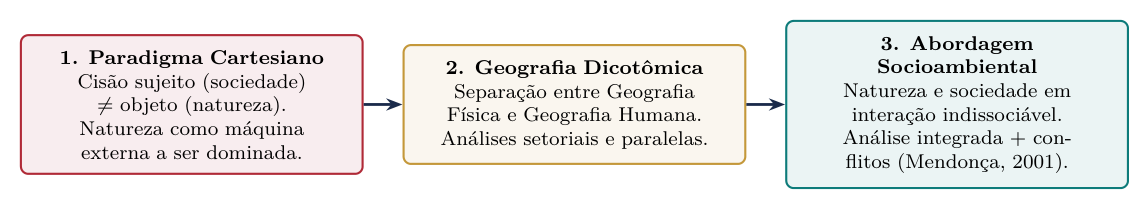
\includegraphics[keepaspectratio,alt={Três quadros conectados mostrando ruptura cartesiana, Geografia dicotômica e abordagem socioambiental}]{capitulos/../img/esquema_sociedade_natureza.png}}

}

\caption{\label{fig-sociedade-natureza}Percurso entre ruptura
cartesiana, divisão disciplinar e abordagem socioambiental. Diagrama do
material da disciplina, recomposto a partir da fonte vetorial original,
com referência a Mendonça (2001).}

\end{figure}%

\subsection{A Natureza como Construção Social e Histórica
(Porto-Gonçalves,
2006)}\label{a-natureza-como-construuxe7uxe3o-social-e-histuxf3rica-porto-gonuxe7alves-2006}

Nas páginas 8 a 36 de \emph{Os (des)caminhos do meio ambiente} (2006),
Carlos Walter Porto-Gonçalves desenvolve uma tese central para a
formação em Geografia, \textbf{toda sociedade e toda cultura cria,
inventa e institui uma determinada ideia do que seja a natureza}. Essa
afirmação merece atenção rigorosa para não ser mal interpretada.

Dizer que a natureza é uma \emph{construção social e histórica} não
significa negar a existência material da chuva, das rochas, da gravidade
ou dos processos biológicos. Significa reconhecer que o modo como os
seres humanos percebem, classificam, valorizam e se relacionam com esses
elementos varia profundamente ao longo da história e entre diferentes
culturas. Na Grécia Antiga pré-socrática, por exemplo, a noção de
\emph{physis} integrava a dimensão física e a existência humana em um
mesmo fluxo; na concepção indígena ou de muitas comunidades tradicionais
brasileiras, rios, serras e matas são territórios de vida, memória e
pertencimento coletivo; já na modernidade capitalista, a natureza é
reduzida predominantemente a mercadoria ou a obstáculo técnico a ser
removido.

Porto-Gonçalves (2006) chama atenção para um paradoxo revelador da
modernidade, ao mesmo tempo em que o sistema urbano-industrial
intensificou a devastação de ecossistemas para expandir a produção de
mercadorias, construiu-se uma visão romantizada de ``natureza
intocada'', definida justamente pela ausência humana. Ambas as posturas
(tanto a exploração predatória quanto o preservacionismo que expulsa
populações tradicionais de seus territórios) compartilham a mesma raiz
cartesiana, a ideia de que sociedade e natureza são polos excludentes.

{\def\LTcaptype{none} % do not increment counter
\begin{longtable}[]{@{}
  >{\raggedright\arraybackslash}p{(\linewidth - 6\tabcolsep) * \real{0.2500}}
  >{\raggedright\arraybackslash}p{(\linewidth - 6\tabcolsep) * \real{0.2500}}
  >{\raggedright\arraybackslash}p{(\linewidth - 6\tabcolsep) * \real{0.2500}}
  >{\raggedright\arraybackslash}p{(\linewidth - 6\tabcolsep) * \real{0.2500}}@{}}
\toprule\noalign{}
\begin{minipage}[b]{\linewidth}\raggedright
\textbf{Matriz Histórico-Cultural}
\end{minipage} & \begin{minipage}[b]{\linewidth}\raggedright
\textbf{Ideia Instituída de Natureza}
\end{minipage} & \begin{minipage}[b]{\linewidth}\raggedright
\textbf{Relação Sociedade-Natureza}
\end{minipage} & \begin{minipage}[b]{\linewidth}\raggedright
\textbf{Expressão Espacial Típica}
\end{minipage} \\
\midrule\noalign{}
\endhead
\bottomrule\noalign{}
\endlastfoot
\textbf{Visões pré-modernas e povos tradicionais} & Totalidade viva,
sagrada ou território de reprodução comunitária. & Pertencimento mútuo;
limites simbólicos e ecológicos ao uso. & Manejo adaptado a ciclos
sazonais (por exemplo, áreas de uso comum no Semiárido). \\
\textbf{Modernidade cartesiana e industrial} & Máquina externa, matéria
mensurável, estoque de recursos. & Separação sujeito-objeto; dominação
técnica e exploração contínua. & Grandes obras, monoculturas,
urbanização acelerada e degradação difusa. \\
\textbf{Preservacionismo excludente} & ``Natureza intocada'', pura
somente onde não há presença humana. & Oposição rígida, toda presença
social é vista como ameaça uniforme. & Ilhas de proteção desconectadas
do entorno e conflitos com comunidades locais. \\
\textbf{Perspectiva socioambiental crítica} & Realidade material e
construção histórico-cultural inseparável da sociedade. & Coexistência
conflituosa e dinâmica mediada por poder, técnica e cultura. &
Planejamento integrado, conservação com justiça territorial e
convivência regional. \\
\end{longtable}
}

\textbf{Tabela 2.1,} Síntese histórica das concepções de natureza e suas
implicações socioespaciais (elaborada com base em Porto-Gonçalves, 2006,
p.~8 a 36).

\subsection{Apropriação dos Recursos Naturais e Racionalidade
Instrumental}\label{apropriauxe7uxe3o-dos-recursos-naturais-e-racionalidade-instrumental}

Sob a modernidade capitalista, os elementos biofísicos da superfície
terrestre passam por um processo sistemático de conversão em
\textbf{recursos naturais}. Esse detalhe conceitual é decisivo na
Geografia, a água, o vento, o solo ou um mineral existem
independentemente da economia, mas só se tornam ``recursos'' quando um
grupo social dispõe de técnica, demanda econômica e respaldo
jurídico-político para se apropriar deles.

Assim, a \textbf{apropriação dos recursos naturais} é sempre guiada por
uma \textbf{racionalidade instrumental}, a técnica é mobilizada não
apenas para satisfazer necessidades humanas básicas, mas para acelerar o
giro do capital, ampliar a escala de extração e reduzir custos privados
de produção. Disso decorre um descompasso estrutural entre duas
temporalidades,

\textbf{Tempo do capital (rápido e linear).} Exige retorno financeiro em
poucos anos, colheitas sucessivas, ampliação rápida de redes energéticas
e expansão contínua sobre novas fronteiras de terra e água.
\textbf{Tempo da natureza (lento e cíclico).} Envolve décadas para
regeneração florestal da Caatinga e do Cerrado, séculos para formação de
centímetros de solo fértil e ciclos plurianuais de recarga de aquíferos
subterrâneos.

\subsection{Natureza, Recurso Natural e Mercadoria, Por que a Distinção
Importa?}\label{natureza-recurso-natural-e-mercadoria-por-que-a-distinuxe7uxe3o-importa}

Ao redigir diagnósticos ambientais, o(a) geógrafo(a) deve distinguir
três níveis, (1) o \textbf{elemento natural} em sua dinâmica biofísica
(por exemplo, o regime de ventos nas serras do Semiárido ou a água
infiltrada em um aquífero); (2) o \textbf{recurso natural}, quando
incorporado por técnicas e finalidades sociais específicas (por exemplo,
potencial eólico mapeado para geração elétrica ou água captada para
irrigação); e (3) a \textbf{mercadoria}, quando esse recurso é
apropriado privadamente e submetido à lógica de compra, venda e
especulação. Grande parte dos conflitos socioambientais nasce exatamente
quando um bem essencial à reprodução comunitária é transformado em
mercadoria excludente.

\subsection{Conflitos Socioambientais e Produção do Espaço na Bahia e no
Nordeste}\label{conflitos-socioambientais-e-produuxe7uxe3o-do-espauxe7o-na-bahia-e-no-nordeste}

A apropriação desigual dos recursos naturais nunca ocorre em um espaço
vazio. Todo território já é ocupado, manejado e significado por
diferentes grupos sociais (comunidades camponesas, quilombolas,
indígenas, pescadores artesanais, agricultores familiares, moradores
urbanos, empresas e Estado). Quando um empreendimento ou política altera
a qualidade do solo, o regime das águas, o acesso à terra ou o modo de
vida local em benefício de determinados agentes e em prejuízo de outros,
emergem \textbf{conflitos socioambientais}.

Um conflito socioambiental não é um mero erro de comunicação nem um
entrave burocrático, trata-se de uma disputa concreta pela
\textbf{produção do espaço geográfico}, na qual diferentes atores
defendem usos incompatíveis ou assimétricos para o mesmo território. No
Nordeste brasileiro e, em especial, no estado da Bahia, quatro frentes
exemplificam de maneira clara essa dinâmica,

\textbf{Expansão energética (parques eólicos no Semiárido Baiano).} A
combinação entre ventos constantes nas serras e chapadas, topografia
favorável e proximidade de linhas de transmissão transformou áreas da
Caatinga baiana, como o eixo de Canudos e regiões serranas do interior
(tema direto da Viagem de Campo da Semana 11), em polo de energia
eólica. Embora frequentemente apresentada apenas como ``energia limpa'',
sua implantação territorial envolve abertura de acessos pesados,
supressão vegetal, compactação e erosão na base das torres, ruído
contínuo, interferência sobre a avifauna local e conflitos fundiários e
contratuais com comunidades rurais (como áreas tradicionais de fundo de
pasto).

\textbf{Barragens e grandes empreendimentos hídricos.} A construção de
reservatórios de grande porte e projetos de regularização fluvial no
Nordeste e na bacia do rio São Francisco reconfigurou profundamente
vales inteiros. Ao lado da geração hidrelétrica e da oferta de água para
polos irrigados, esses projetos frequentemente implicaram o alagamento
de terras férteis de vazante, o deslocamento compulsório de populações
ribeirinhas, a alteração do regime natural de cheias e vazantes e
mudanças na dinâmica hidrossedimentológica a jusante (com impacto sobre
a pesca artesanal e a erosão marginal).

\textbf{Fronteira agrícola (Oeste Baiano / domínio do Cerrado).} A
expansão acelerada da agricultura mecanizada intensiva sobre os
chapadões do Oeste Baiano reestruturou a economia regional, mas gerou
forte pressão sobre a vegetação nativa de Cerrado, sobre áreas
estratégicas de recarga hídrica (associadas ao sistema Aquífero Urucuia)
e sobre vazões de rios afluentes. Esse avanço desencadeou disputas
territoriais pelo uso da terra e da água envolvendo comunidades
tradicionais geraizeiras e de fecho de pasto.

\textbf{Acesso desigual à água no Semiárido.} Historicamente, políticas
centradas no ``combate à seca'' privilegiaram grandes açudes e obras
concentradas em propriedades privadas ou voltadas a setores econômicos
específicos, mantendo populações rurais dependentes de carros-pipa em
períodos de estiagem. Em contraposição, movimentos sociais,
universidades e instituições públicas vêm consolidando estratégias de
\textbf{convivência com o Semiárido}, articulando tecnologias sociais
descentralizadas (como cisternas de captação de água de chuva), manejo
conservacionista do solo e democratização da gestão hídrica.

{\def\LTcaptype{none} % do not increment counter
\begin{longtable}[]{@{}
  >{\raggedright\arraybackslash}p{(\linewidth - 8\tabcolsep) * \real{0.2000}}
  >{\raggedright\arraybackslash}p{(\linewidth - 8\tabcolsep) * \real{0.2000}}
  >{\raggedright\arraybackslash}p{(\linewidth - 8\tabcolsep) * \real{0.2000}}
  >{\raggedright\arraybackslash}p{(\linewidth - 8\tabcolsep) * \real{0.2000}}
  >{\raggedright\arraybackslash}p{(\linewidth - 8\tabcolsep) * \real{0.2000}}@{}}
\toprule\noalign{}
\begin{minipage}[b]{\linewidth}\raggedright
\textbf{Frente Espacial (BA/NE)}
\end{minipage} & \begin{minipage}[b]{\linewidth}\raggedright
\textbf{Recurso Apropriado}
\end{minipage} & \begin{minipage}[b]{\linewidth}\raggedright
\textbf{Atores em Disputa}
\end{minipage} & \begin{minipage}[b]{\linewidth}\raggedright
\textbf{Impactos Físico-Bióticos Associados}
\end{minipage} & \begin{minipage}[b]{\linewidth}\raggedright
\textbf{Tensão Socioespacial Central}
\end{minipage} \\
\midrule\noalign{}
\endhead
\bottomrule\noalign{}
\endlastfoot
\textbf{Expansão eólica (Semiárido)} & Vento, serras e áreas de
Caatinga. & Empresas de energia, proprietários, comunidades rurais e
fundo de pasto. & Supressão vegetal, erosão na base das torres,
compactação de acessos e impacto na avifauna. & Contratos de
arrendamento assimétricos, ruído e restrição de usos comuns. \\
\textbf{Barragens e obras hídricas} & Vazão fluvial, vales aluviais e
energia potencial. & Setor elétrico/irrigação, Estado e populações
ribeirinhas/pescadores. & Submersão de várzeas, alteração do regime
fluvial e retenção de sedimentos. & Deslocamento compulsório, perda de
terras de vazante e desestruturação comunitária. \\
\textbf{Fronteira agrícola (Oeste Baiano)} & Solos planos de Cerrado e
águas superficiais/subterrâneas. & Agronegócio mecanizado, Estado e
comunidades geraizeiras/fecho de pasto. & Desmatamento de áreas de
recarga, alta extração hídrica e exposição edáfica. & Cercamento de
terras tradicionais e conflito pela disponibilidade hídrica. \\
\textbf{Acesso à água (Semiárido)} & Águas superficiais, nascentes e
reservatórios. & Grandes usuários, poder público e agricultores
familiares. & Assoreamento, degradação ciliar e sobre-exploração em
estiagens. & Concentração hídrica (``combate à seca'')
vs.~democratização (``convivência''). \\
\end{longtable}
}

\textbf{Tabela 2.2,} Matriz analítica de conflitos socioambientais
representativos da Bahia e do Nordeste na perspectiva da produção do
espaço geográfico.

\subsection{Introdução à Abordagem Socioambiental na Geografia
(Mendonça,
2001)}\label{introduuxe7uxe3o-uxe0-abordagem-socioambiental-na-geografia-mendonuxe7a-2001}

Diante das limitações do dualismo cartesiano e da intensidade dos
conflitos territoriais contemporâneos, a Geografia brasileira
desenvolveu esforços consistentes para superar a separação entre o
estudo da natureza e o estudo da sociedade. Um marco fundamental desse
movimento é o artigo \emph{Geografia socioambiental}, publicado por
Francisco Mendonça na revista \emph{Terra Livre} (n.~16, 2001, p.~139 a
158).

Mendonça (2001) questiona o uso genérico do termo ``ambiental'' quando
este aparece reduzido exclusivamente à esfera natural (relevo, clima,
fauna, flora), sem incorporar os sujeitos históricos, a desigualdade
social e as relações de poder. Por isso, o autor defende a adoção
deliberada do prefixo \textbf{``socio-''} na expressão \textbf{Geografia
Socioambiental}, trata-se de afirmar, desde a própria denominação, que
os problemas ambientais só podem ser compreendidos na interação
dialética entre natureza e sociedade.

Essa introdução à abordagem socioambiental estabelece três princípios
metodológicos que serão aprofundados no Capítulo 3,

\textbf{Superação da dicotomia físico-humano.} Não se trata de anular as
especificidades da geomorfologia, da climatologia ou da geografia
agrária, mas de articulá-las diante de problemas concretos em que
processos naturais e sociais se co-produzem. \textbf{Centralidade da
sociedade na problemática ambiental.} Enchentes urbanas, erosão
acelerada, desertificação ou escassez hídrica não atingem todos os
grupos sociais igualmente; sua gravidade depende da vulnerabilidade
social e da organização desigual do espaço.

\textbf{Compromisso com o diagnóstico e a intervenção territorial.} A
Geografia Socioambiental combina rigor teórico-metodológico com
relevância social, orientando diagnósticos ambientais que subsidiem
políticas públicas, licenciamento e recuperação de áreas degradadas.

\subsection{Ponte Direta para o Estudo Orientado 1 (EO1) e o Capítulo
3}\label{ponte-direta-para-o-estudo-orientado-1-eo1-e-o-capuxedtulo-3}

O \textbf{Estudo Orientado 1 (EO1)} avalia sua capacidade de articular a
leitura de Porto-Gonçalves (2006, p.~8 a 36) e a introdução a Mendonça
(2001). Ao redigir seu texto, mostre com clareza, (1) como a modernidade
separou sociedade e natureza; (2) por que a ideia de natureza é
historicamente construída; (3) como a apropriação instrumental dos
recursos produz conflitos socioambientais concretos; e (4) por que a
abordagem socioambiental supera visões puramente naturalistas. No
Capítulo 3, você aprofundará o texto de Mendonça (2001) junto ao modelo
geográfico de Bertrand (2004).

\subsection{Conhecimento, apropriação e conflito no uso da
água}\label{conhecimento-apropriauxe7uxe3o-e-conflito-no-uso-da-uxe1gua}

Uma barragem modifica o armazenamento e a circulação da água, mas sua
análise também envolve a definição das prioridades de uso. A cota de
operação, os períodos de liberação e as regras de acesso aos pontos de
captação resultam de decisões institucionais. Essas decisões alteram as
condições de pesca, abastecimento, irrigação e produção de energia, com
efeitos diferentes sobre grupos situados a montante e a jusante.

O estudo de um conflito exige reconstruir essas relações. A
caracterização física deve informar o comportamento das vazões e os
períodos de menor disponibilidade, enquanto a investigação social
identifica os usuários, as formas de acesso e as instâncias de
negociação. Entrevistas precisam registrar a posição e o período de
observação de cada participante, permitindo distinguir experiência
local, interpretação e informação documental.

A explicação final articula o funcionamento hídrico às regras que
distribuem seu uso. Uma estiagem pode reduzir a oferta, enquanto
desigualdades na infraestrutura e nas autorizações ampliam seus efeitos
sobre determinados usuários. Essa relação permite formular intervenções
mais precisas, como melhorar a captação, rever regras de alocação ou
recuperar áreas que contribuem para a qualidade da água.

\section{Etapa 4 - Exemplos
resolvidos}\label{etapa-4---exemplos-resolvidos-1}

\emph{Nota metodológica,} Os casos abaixo combinam processos espaciais
reais da Bahia e do Nordeste com \textbf{cenários didáticos
ilustrativos} (números, nomes de localidades e parâmetros estilizados)
criados para exercitar a análise crítica baseada em Porto-Gonçalves
(2006) e Mendonça (2001).

\subsection{Exemplo 2.1, Básico. Identificando o Dualismo Cartesiano em
um Relatório
Ambiental}\label{exemplo-2.1-buxe1sico.-identificando-o-dualismo-cartesiano-em-um-relatuxf3rio-ambiental}

\textbf{Situação analisada.} Para criar uma unidade de conservação de
proteção integral em uma serra fictícia da Bahia \emph{(cenário didático
ilustrativo)}, uma consultoria entregou um relatório técnico dividido em
duas partes sem conexão, o Volume 1 descreve a flora e as nascentes como
``patrimônio natural puro'', e o Volume 2 recomenda a retirada imediata
de 35 famílias que vivem há três gerações na área praticando
extrativismo de baixa intensidade e manejo comunitário de pastagens,
classificando qualquer presença humana como ``fator de destruição da
natureza''.

\textbf{Dados disponíveis.} Relatório dividido em dois volumes isolados;
idealização da área como ``natureza pura''; recomendação de remoção de
35 famílias tradicionais sem avaliar seus modos históricos de manejo.

\textbf{Problema a resolver.} Identificar qual concepção de natureza
fundamenta o relatório à luz de Porto-Gonçalves (2006) e explicar por
que essa postura reproduz o dualismo moderno.

\textbf{Fundamento da análise.} Análise epistemológica das concepções de
natureza e do paradoxo preservacionista excludente em Porto-Gonçalves
(2006, p.~8 a 36).

\textbf{Desenvolvimento.}

\textbf{Identificação da concepção subjacente.} O relatório adota o mito
da ``natureza intocada'', definindo o natural exclusivamente pela
ausência de seres humanos. \textbf{Raiz cartesiana (Porto-Gonçalves,
2006).} Embora aparente opor-se à exploração predatória, essa visão
parte da mesma ruptura moderna que separa rigidamente sociedade e
natureza em polos excludentes. \textbf{Equívoco geográfico e social.} Ao
tratar todas as formas de presença humana como igualmente destrutivas, a
consultoria ignora que os modos de manejo tradicional dessas 35 famílias
podem ter contribuído justamente para conservar a cobertura vegetal e as
nascentes ao longo de gerações, gerando um conflito socioambiental
desnecessário.

\textbf{Interpretação do resultado.} O relatório fundamenta-se na
concepção dicotômica da ``natureza intocada'', herdeira da ruptura
cartesiana entre sociedade e natureza, ao opor automaticamente
conservação ambiental e presença de populações tradicionais.

\textbf{Condições de validade.} A crítica é coerente com a Análise
Ambiental contemporânea, conservar nascentes exige avaliar empiricamente
o impacto real de cada prática de uso da terra, diferenciando manejo
comunitário de baixo impacto de pressões predatórias externas.

\subsection{Exemplo 2.2, Básico. Da Natureza ao Recurso Natural, o Vento
nas Serras do
Semiárido}\label{exemplo-2.2-buxe1sico.-da-natureza-ao-recurso-natural-o-vento-nas-serras-do-semiuxe1rido}

\textbf{Situação analisada.} Durante décadas, os ventos intensos que
sopram no topo de uma serra da Caatinga \emph{(cenário didático
ilustrativo)} eram percebidos pelos moradores locais apenas como parte
do clima cotidiano, influenciando a secagem do solo e o manejo dos
rebanhos em áreas de uso comum. Nos últimos cinco anos, após o avanço de
turbinas de grande porte, o mapeamento anemométrico e a instalação de
uma subestação elétrica próxima, o mesmo vento passou a atrair grandes
investimentos e contratos de arrendamento de terras para implantação de
um complexo eólico.

\textbf{Dados disponíveis.} Elemento biofísico preexistente, regime de
ventos intensos na serra. Novos fatores históricos/técnicos,
aerogeradores de grande porte, mapeamento de potencial eólico e
proximidade de linhas de transmissão. Consequência, revalorização
fundiária e contratos de arrendamento.

\textbf{Problema a resolver.} Explicar, com base na distinção entre
\emph{elemento natural} e \emph{recurso natural}, por que o vento
adquiriu valor econômico territorial apenas recentemente e quais tensões
socioambientais podem emergir.

\textbf{Fundamento da análise.} Análise geográfica do processo de
apropriação dos recursos naturais e da produção do espaço sob
racionalidade instrumental.

\textbf{Desenvolvimento.}

\textbf{De elemento natural a recurso.} O vento sempre existiu
fisicamente na serra, mas só se converteu em \emph{recurso energético}
quando condições técnicas (aerogeradores), infraestruturais (linhas de
transmissão) e econômicas (mercado de energia) permitiram sua
apropriação rentável. \textbf{Reconfiguração espacial.} A implantação
das torres exige estradas de acesso largas, bases de concreto e faixas
de servidão, o que altera a cobertura de Caatinga, expõe o solo à erosão
na base das torres e interfere na avifauna.

\textbf{Tensões socioambientais emergentes.} O cercamento de áreas antes
usadas coletivamente, a assimetria na negociação de contratos de
arrendamento e o desconforto acústico próximo às moradias transformam um
projeto de ``energia renovável'' em arena de conflito territorial se não
houver planejamento socioambiental justo.

\textbf{Interpretação do resultado.} O vento tornou-se recurso natural
apenas quando incorporado por um conjunto técnico, infraestrutural e
econômico específico; sua apropriação reorganiza o território da serra e
pode gerar impactos físicos e conflitos fundiários com comunidades
locais.

\textbf{Condições de validade.} O exemplo demonstra uma lição-chave para
a viagem de campo da Semana 11 (eixo de Canudos), ser fonte renovável
não torna um empreendimento isento de impactos ambientais ou conflitos
territoriais.

\subsection{Exemplo 2.3, Intermediário. Balanço Hídrico Didático e
Conflito Socioambiental em Açude
Semiárido}\label{exemplo-2.3-intermediuxe1rio.-balanuxe7o-huxeddrico-diduxe1tico-e-conflito-socioambiental-em-auxe7ude-semiuxe1rido}

\textbf{Situação analisada.} Em uma microbacia semiárida fictícia
\emph{(cenário didático ilustrativo)}, um açude público possui volume
útil estimado de \(120.000\text{ m}^3\) ao final da estação chuvosa,
destinado a atender à demanda de 8 meses de estiagem (240 dias). O
reservatório abastece 250 famílias de agricultores familiares (consumo
médio estimado de \(0,5\text{ m}^3/\text{dia}\) por família para usos
domésticos e dessedentação de pequenos animais) e também passou a sofrer
captação de um empreendimento privado de irrigação intensiva instalado a
montante, que demanda \(450\text{ m}^3/\text{dia}\). Desconsidere, neste
exercício inicial, a evaporação direta para focar no balanço das
demandas humanas.

\textbf{Dados disponíveis.} Volume útil disponível,
\(V_{\text{disp}} = 120.000\text{ m}^3\); período de estiagem,
\(T = 240\text{ dias}\); demanda comunitária,
\(250\text{ famílias} \times 0,5\text{ m}^3/(\text{família}\cdot\text{dia})\);
demanda do empreendimento privado, \(450\text{ m}^3/\text{dia}\).

\textbf{Problema a resolver.} (a) Calcular a demanda total de cada grupo
nos 240 dias e verificar se o volume disponível suporta ambos os usos
simultaneamente; (b) interpretar o resultado como um conflito
socioambiental pelo acesso à água.

\textbf{Fundamento da análise.} Cálculo passo a passo de balanço
volumétrico simples (\(V = Q \times T\)) articulado à análise geográfica
de conflitos socioambientais e racionalidade instrumental.

\textbf{Desenvolvimento.}

\textbf{Demanda diária e total das 250 famílias comunitárias,}

\[
Q_{\text{fam}} = 250 \times 0{,}5 = 125\text{ m}^3/\text{dia}
\]

\[
V_{\text{fam}} = 125\text{ m}^3/\text{dia} \times 240\text{ dias} = 30.000\text{ m}^3
\]

. \textbf{Demanda total do empreendimento privado de irrigação,}

\[
V_{\text{priv}} = 450\text{ m}^3/\text{dia} \times 240\text{ dias} = 108.000\text{ m}^3
\]

. \textbf{Demanda conjunta e saldo hídrico,}

\[
V_{\text{total}} = V_{\text{fam}} + V_{\text{priv}} = 30.000 + 108.000 = 138.000\text{ m}^3
\]

\[
\text{Saldo} = V_{\text{disp}} - V_{\text{total}} = 120.000 - 138.000 = -18.000\text{ m}^3 \quad (\text{déficit de } 18.000\text{ m}^3)
\]

. \textbf{Participação percentual nas demandas,} As 250 famílias
respondem por \(\frac{30.000}{138.000} \times 100\% \approx 21,7\%\) da
demanda total (e consumiriam apenas \(25\%\) do volume útil do açude),
enquanto o único empreendimento privado responde por
\(\frac{108.000}{138.000} \times 100\% \approx 78,3\%\) (exigindo
sozinho \(90\%\) de toda a água armazenada). \textbf{Interpretação
socioambiental.} O déficit de \(18.000\text{ m}^3\) não decorre de falta
absoluta de água para a população local (o açude atenderia quatro vezes
a necessidade básica das 250 famílias), mas da apropriação concentrada
do recurso sob racionalidade instrumental. Como a evaporação real no
Semiárido ainda reduziria o volume disponível, o colapso do
abastecimento humano ocorreria ainda antes do fim dos 240 dias.

\textbf{Interpretação do resultado.} As demandas somam
\(138.000\text{ m}^3\) frente a \(120.000\text{ m}^3\) disponíveis,
gerando déficit de \(18.000\text{ m}^3\). O empreendimento privado
concentra \(78,3\%\) da demanda, caracterizando um conflito
socioambiental distributivo pelo uso da água.

\textbf{Condições de validade.} Verificação física e institucional, a
soma \(30.000 + 108.000 = 138.000\text{ m}^3\) confirma o déficit; além
disso, pela Política Nacional de Recursos Hídricos (Lei nº 9.433/1997),
em situações de escassez, o uso prioritário dos recursos hídricos é o
consumo humano e a dessedentação de animais, o que reforça a
ilegitimidade de sacrificar o abastecimento das 250 famílias.

\subsection{Exemplo 2.4, Intermediário. Expansão da Fronteira Agrícola e
Abordagem Socioambiental no Cerrado
Baiano}\label{exemplo-2.4-intermediuxe1rio.-expansuxe3o-da-fronteira-agruxedcola-e-abordagem-socioambiental-no-cerrado-baiano}

\textbf{Situação analisada.} Em uma sub-bacia fictícia de chapadão no
Oeste Baiano \emph{(cenário didático ilustrativo)}, com área total de
\(40.000\text{ ha}\), o mapeamento de cobertura vegetal mostrou que, em
15 anos, a vegetação nativa de Cerrado reduziu-se de
\(32.000\text{ ha}\) para \(14.000\text{ ha}\), substituída por lavouras
mecanizadas irrigadas por pivôs centrais. Paralelamente, comunidades de
fecho de pasto situadas nos vales a jusante relatam redução na vazão de
veredas que utilizavam para cultivo de subsistência e criação extensiva.

\textbf{Dados disponíveis.} Área da sub-bacia, \(40.000\text{ ha}\);
Cerrado nativo caiu de \(32.000\text{ ha}\) para \(14.000\text{ ha}\) em
15 anos; expansão de pivôs centrais no topo do chapadão; redução de
vazão em veredas usadas por comunidades de fecho de pasto a jusante.

\textbf{Problema a resolver.} (a) Calcular a área convertida e o
percentual da sub-bacia que perdeu vegetação nativa nesse intervalo; (b)
construir uma leitura integrada do caso segundo a Geografia
Socioambiental de Mendonça (2001).

\textbf{Fundamento da análise.} Quantificação da conversão de cobertura
vegetal seguida de análise dialética entre dinâmica físico-hidrológica
(recarga no chapadão e descarga nas veredas) e conflito territorial
(Mendonça, 2001).

\textbf{Desenvolvimento.}

\textbf{Quantificação da perda de Cerrado,}

\[
\Delta A = 14.000 - 32.000 = -18.000\text{ ha}
\]

Percentual da sub-bacia convertido no período,
\(\frac{18.000}{40.000} \times 100\% = 45,0\%\) da área total.
Percentual de perda sobre o Cerrado inicial,
\(\frac{18.000}{32.000} \times 100\% = 56,25\%\) da vegetação nativa
existente no início do período. \textbf{Leitura físico-hidrológica
integrada.} Os chapadões arenosos do Cerrado funcionam como áreas
estratégicas de infiltração e recarga subterrânea que alimentam
nascentes e veredas nos vales. A conversão de \(45\%\) da sub-bacia
associada à captação intensiva por pivôs centrais altera o balanço
hídrico local e reduz a contribuição para os cursos d'água a jusante.

\textbf{Leitura socioambiental (Mendonça, 2001).} Uma análise puramente
física mediria apenas a vazão das veredas, e uma análise puramente
social descreveria apenas a disputa por terras sem compreender a
conectividade hidrológica entre chapadão e vale. A Geografia
Socioambiental une ambos os planos, demonstra que a produção do espaço
pelo agronegócio intensivo no topo da bacia transfere custos hídricos e
vulnerabilidade social para as comunidades tradicionais nos fundos de
vale.

\textbf{Interpretação do resultado.} Foram convertidos
\(18.000\text{ ha}\) (\(45,0\%\) da sub-bacia e \(56,25\%\) do Cerrado
inicial). Sob a Geografia Socioambiental (Mendonça, 2001), o
rebaixamento das veredas evidencia a inseparabilidade entre
conectividade hidrológica chapadão-vale e apropriação desigual do
território.

\textbf{Condições de validade.} Os cálculos fecham
(\(32.000 - 18.000 = 14.000\text{ ha}\), restando \(35\%\) da sub-bacia
com Cerrado nativo), e a interpretação respeita a lógica de bacia
hidrográfica ao conectar uso do solo em área de recarga com impactos
socioespaciais a jusante.

\subsection{Exemplo 2.5, Avançado. Barragem Fluvial, Descompasso de
Temporalidades e Conflito
Territorial}\label{exemplo-2.5-avanuxe7ado.-barragem-fluvial-descompasso-de-temporalidades-e-conflito-territorial}

\textbf{Situação analisada.} A construção de uma barragem de médio porte
em um vale fluvial nordestino \emph{(cenário didático ilustrativo)}
regularizou a vazão do rio para garantir geração elétrica e fornecimento
constante a um perímetro agroindustrial. Cinco anos após o enchimento do
reservatório, observam-se três efeitos encadeados, (i) comunidades
ribeirinhas reassentadas em terrenos secos afastados do rio perderam a
prática secular da agricultura de vazante; (ii) a retenção de sedimentos
no reservatório reduziu a deposição natural de nutrientes nas várzeas a
jusante e intensificou a erosão das margens; e (iii) a pesca artesanal
declinou devido à barreira física à migração de peixes e à
homogeneização do pulso de cheias.

\textbf{Dados disponíveis.} Obra de regularização fluvial voltada à
geração elétrica e irrigação intensiva; três efeitos após 5 anos, perda
da agricultura de vazante pós-reassentamento, retenção de sedimentos com
erosão marginal a jusante e declínio da pesca artesanal.

\textbf{Problema a resolver.} Analisar o caso integrando, (a) a
racionalidade instrumental e o descompasso entre tempo do capital e
tempo ecológico; (b) a concepção de natureza subjacente à obra
(Porto-Gonçalves, 2006); e (c) diretrizes de diagnóstico sob a ótica da
Geografia Socioambiental (Mendonça, 2001).

\textbf{Fundamento da análise.} Síntese teórico-metodológica articulando
Porto-Gonçalves (2006, p.~8 a 36), Mendonça (2001) e processos
hidrossedimentológicos fluviais básicos.

\textbf{Desenvolvimento.}

\textbf{Racionalidade instrumental e temporalidades.} O projeto tratou o
rio sob o tempo linear e contínuo da produção industrial (vazão
regularizada o ano inteiro), suprimindo o pulso sazonal de cheias e
vazantes que estruturava tanto o ecossistema aquático (reprodução de
peixes e renovação sedimentar das várzeas) quanto o calendário agrícola
das famílias ribeirinhas. \textbf{Concepção moderna de natureza
(Porto-Gonçalves, 2006).} O rio foi concebido como mera tubulação
hidráulica ou estoque de energia potencial a ser domado pela engenharia,
ignorando que, para os ribeirinhos, ele constitui um território de vida
historicamente construído. O reassentamento em terras secas pressupôs
que ``qualquer lote de terra substitui outro'', apagando a
especificidade ecológica e cultural da várzea.

\textbf{Diretrizes de diagnóstico socioambiental (Mendonça, 2001).} Um
diagnóstico rigoroso deve, (a) avaliar a bacia inteira (montante,
reservatório e jusante), incorporando o balanço de sedimentos e a
estabilidade das margens; (b) mapear territorialidades tradicionais e
dependência direta dos pulsos hidrológicos antes da decisão de
licenciamento; (c) propor regras de operação de vazões ambientais
(hidrograma ecológico) e medidas reais de reparação territorial e
participação comunitária na gestão do reservatório.

\textbf{Interpretação do resultado.} O caso evidencia como a
racionalidade instrumental transforma um sistema fluvial vivo em
infraestrutura setorial, rompendo simultaneamente processos
hidrossedimentológicos e modos de vida ribeirinhos; a Geografia
Socioambiental exige diagnosticar a bacia de forma integrada e
reconhecer os sujeitos territoriais afetados.

\textbf{Condições de validade.} A análise confirma a interdependência
entre físico e social, a retenção de sedimentos pela barragem (processo
geomorfológico) não só gera erosão marginal a jusante, como empobrece
várzeas e compromete a segurança alimentar e a renda das comunidades.

\section{Etapa 5 - Erros de
interpretação}\label{etapa-5---erros-de-interpretauxe7uxe3o-1}

\subsection{Erro 2.1, Confundir ``Natureza como Construção Social'' com
Negação da Materialidade
Física}\label{erro-2.1-confundir-natureza-como-construuxe7uxe3o-social-com-negauxe7uxe3o-da-materialidade-fuxedsica}

\textbf{Equívoco frequente.} Interpretar a tese de Porto-Gonçalves
(2006) como se a erosão, as chuvas ou os processos geológicos fossem
apenas ``invenções da mente humana'' sem realidade material.

\textbf{Por que está incorreto.} A materialidade biofísica existe
objetivamente e obedece a leis físicas, químicas e biológicas. O que é
social e historicamente construído é a \emph{ideia} de natureza, o
significado cultural que lhe atribuímos e as formas técnicas e
econômicas pelas quais a apropriamos e transformamos.

\textbf{Como evitar.} Afirme sempre a dupla dimensão, os processos
naturais possuem dinâmica material própria, mas sua apropriação,
valoração e interpretação são mediadas pela história e pela sociedade.

\subsection{Erro 2.2, Tratar Conflitos Socioambientais como ``Falta de
Diálogo'' ou ``Resistência ao
Progresso''}\label{erro-2.2-tratar-conflitos-socioambientais-como-falta-de-diuxe1logo-ou-resistuxeancia-ao-progresso}

\textbf{Equívoco frequente.} Explicar a oposição de comunidades rurais
ou ribeirinhas a grandes obras (barragens, parques energéticos,
fronteira agrícola) como ``desinformação'' ou ``atraso cultural''.

\textbf{Por que está incorreto.} Conflitos socioambientais expressam
disputas concretas e legítimas por água, solo, território, saúde e
reprodução social. Rotular populações afetadas como ``contra o
progresso'' oculta assimetrias de poder e a distribuição desigual de
custos e benefícios.

\textbf{Como evitar.} Identifique em todo conflito os atores envolvidos,
os recursos disputados, os impactos físico-bióticos diferenciados e os
projetos de território em confronto.

\subsection{Erro 2.3, Reproduzir o Mito da ``Natureza Intocada'' na
Conservação
Ambiental}\label{erro-2.3-reproduzir-o-mito-da-natureza-intocada-na-conservauxe7uxe3o-ambiental}

\textbf{Equívoco frequente.} Supor que toda presença humana degrada o
ambiente na mesma medida e que conservar significa necessariamente
esvaziar territórios de seus habitantes tradicionais.

\textbf{Por que está incorreto.} Como aponta Porto-Gonçalves (2006),
essa postura reproduz a cisão cartesiana entre humano e natural,
equiparando sistemas comunitários de baixo impacto a empreendimentos
industriais de alta degradação.

\textbf{Como evitar.} Analise empiricamente as práticas reais de uso da
terra e reconheça que populações tradicionais frequentemente atuam como
guardiãs da sociobiodiversidade.

\subsection{Erro 2.4, Reduzir a Geografia Socioambiental à Justaposição
de Física e
Humana}\label{erro-2.4-reduzir-a-geografia-socioambiental-uxe0-justaposiuxe7uxe3o-de-fuxedsica-e-humana}

\textbf{Equívoco frequente.} Acreditar que aplicar Mendonça (2001)
consiste em escrever uma seção sobre clima e solo e outra seção
independente sobre população e economia.

\textbf{Por que está incorreto.} Justapor capítulos paralelos mantém
intacta a dicotomia clássica da Geografia. A abordagem socioambiental
exige mostrar como processos naturais e dinâmicas sociais interagem e se
modificam reciprocamente no mesmo espaço.

\textbf{Como evitar.} Formule suas análises a partir de nexos causais
integrados (por exemplo, como o modelo de ocupação de uma encosta ou
bacia altera processos erosivos e concentra riscos sobre grupos
vulneráveis).

\section{Etapa 6 - Exercícios de
fixação}\label{etapa-6---exercuxedcios-de-fixauxe7uxe3o-1}

\subsubsection{Nível 1, Básicos (Compreensão
Conceitual)}\label{nuxedvel-1-buxe1sicos-compreensuxe3o-conceitual-1}

\begin{enumerate}
\def\labelenumi{\arabic{enumi}.}
\item
  Explique em que consiste a \emph{ruptura cartesiana} entre sociedade e
  natureza na modernidade e aponte uma consequência direta dessa cisão
  para a organização da Geografia clássica.
\item
  Com base em Porto-Gonçalves (2006, p.~8 a 36), esclareça o significado
  da afirmação de que a natureza é uma \emph{construção social e
  histórica}, cuidando para não negar a materialidade dos processos
  físicos.
\item
  Diferencie \emph{elemento natural} de \emph{recurso natural},
  ilustrando com um exemplo concreto da realidade baiana ou nordestina.
\item
  Explique o descompasso entre o \emph{tempo do capital} e o \emph{tempo
  da natureza} no contexto da racionalidade instrumental moderna.
\item
  Segundo Francisco Mendonça (2001), qual é a justificativa teórica e
  metodológica para o uso do prefixo ``socio-'' na expressão
  \emph{Geografia Socioambiental}?

  \#\#\#\# Nível 2, Intermediários (Análise Crítica e Aplicação)
\item
  Analise o paradoxo apontado por Porto-Gonçalves (2006) entre a
  exploração predatória da natureza como mercadoria e a defesa de uma
  ``natureza intocada'' sem presença humana. O que essas duas visões têm
  em comum?
\item
  Escolha uma das quatro frentes de conflito socioambiental discutidas
  no capítulo (expansão eólica no Semiárido, barragens fluviais,
  fronteira agrícola no Oeste Baiano ou acesso desigual à água) e
  identifique, (a) o recurso apropriado; (b) os principais atores em
  disputa; e (c) dois impactos físico-bióticos articulados a efeitos
  sociais.
\item
  Em um cenário didático ilustrativo, um reservatório comunitário no
  Semiárido dispõe de \(90.000\text{ m}^3\) de volume útil para 200 dias
  de estiagem. Duas demandas disputam essa água, 150 famílias que
  consomem \(0,6\text{ m}^3/\text{dia}\) cada e um empreendimento
  externo que solicita autorização para captar
  \(400\text{ m}^3/\text{dia}\). Calcule a demanda total de cada parte
  no período, verifique se há déficit e analise o caso sob a ótica dos
  conflitos socioambientais.
\item
  Diferencie as políticas históricas de ``combate à seca'' das
  estratégias contemporâneas de ``convivência com o Semiárido'',
  relacionando essa distinção à racionalidade instrumental e à justiça
  socioambiental.
\item
  Elabore um parágrafo analítico demonstrando como a abordagem
  socioambiental (Mendonça, 2001) supera tanto o naturalismo redutor
  quanto o sociologismo que ignora o suporte físico-biótico do
  território.

  \subsubsection{Nível 3, Aplicados e Objetivos (Múltipla
  Escolha)}\label{nuxedvel-3-aplicados-e-objetivos-muxfaltipla-escolha-1}
\item
  Na análise de Porto-Gonçalves (2006, p.~8 a 36) sobre a formação
  histórica da questão ambiental na modernidade, a separação entre
  sociedade e natureza,

  \begin{enumerate}
  \def\labelenumii{(\Alph{enumii})}
  \item
    É uma característica biológica universal presente de forma idêntica
    em todas as culturas humanas desde a pré-história.
  \item
    Consolida-se historicamente com o pensamento moderno-cartesiano,
    instituindo a natureza como objeto externo e passivo a ser dominado
    pela ciência e pela técnica.
  \item
    Foi completamente superada pela Revolução Industrial, que reintegrou
    o ritmo produtivo das fábricas aos ciclos lentos dos ecossistemas.
  \item
    Refere-se exclusivamente à divisão administrativa entre zonas
    urbanas e zonas rurais nos municípios brasileiros.
  \item
    Impediu o desenvolvimento das ciências da natureza, pois o
    mecanicismo cartesiano rejeitava qualquer estudo matemático do mundo
    físico.
  \end{enumerate}
\item
  Sobre o processo pelo qual um elemento biofísico passa a ser tratado
  como \emph{recurso natural}, é \textbf{correto} afirmar que,

  \begin{enumerate}
  \def\labelenumii{(\Alph{enumii})}
  \item
    Todo elemento físico da crosta terrestre é automaticamente um
    recurso econômico, independentemente da técnica ou da organização
    social existente.
  \item
    A transformação de elementos da natureza em recursos naturais
    depende de condições técnicas, econômicas, culturais e políticas
    historicamente situadas.
  \item
    Recursos renováveis, como o vento e a energia solar, jamais geram
    impactos ambientais ou conflitos territoriais quando apropriados em
    larga escala.
  \item
    A apropriação de recursos naturais sob racionalidade instrumental
    respeita integralmente o tempo geológico de formação dos solos e de
    recarga dos aquíferos.
  \item
    A noção de recurso natural é neutra e alheia às disputas fundiárias
    ou à produção do espaço geográfico.
  \end{enumerate}
\item
  No contexto da Bahia e do Nordeste, a expansão de parques eólicos em
  áreas serranas da Caatinga exemplifica um conflito socioambiental
  porque,

  \begin{enumerate}
  \def\labelenumii{(\Alph{enumii})}
  \item
    A geração eólica produz grandes volumes de gases de efeito estufa
    diretamente na atmosfera do Semiárido durante a rotação das pás.
  \item
    Embora utilize fonte renovável, a apropriação espacial das serras
    provoca supressão vegetal, erosão na base das torres, interferência
    na avifauna e tensões fundiárias com comunidades locais.
  \item
    Os ventos do Semiárido são insuficientes para movimentar turbinas,
    tornando a região tecnicamente inviável para energia eólica.
  \item
    As comunidades locais opõem-se por princípio a qualquer forma de
    energia elétrica, recusando-se a utilizar eletricidade em suas
    residências.
  \item
    Os impactos físicos das obras restringem-se ao interior das
    subestações urbanas, sem atingir o relevo, os solos ou a vegetação
    da Caatinga.
  \end{enumerate}
\item
  De acordo com a proposta de \emph{Geografia Socioambiental} formulada
  por Francisco Mendonça (2001),

  \begin{enumerate}
  \def\labelenumii{(\Alph{enumii})}
  \item
    O estudo ambiental deve restringir-se aos fenômenos climáticos e
    geomorfológicos naturais, evitando interferência de temas sociais e
    políticos.
  \item
    A Geografia Física deve ser extinta dos cursos de graduação, pois
    apenas a análise econômica explica a degradação do espaço.
  \item
    A incorporação do termo ``socioambiental'' busca superar a dicotomia
    físico-humano, compreendendo o ambiente a partir da interação
    indissociável entre natureza e sociedade.
  \item
    Os desastres e a degradação ambiental atingem de maneira uniforme
    todas as classes sociais, independentemente da organização do
    território.
  \item
    A abordagem socioambiental consiste em anexar um capítulo de
    demografia ao final de relatórios geomorfológicos sem estabelecer
    relações causais entre eles.
  \end{enumerate}
\item
  Em um cenário didático ilustrativo, uma comunidade tradicional de
  fundo de pasto e uma empresa agroindustrial disputam o uso das águas
  de um riacho que nasce em área de chapadão. A análise desse episódio
  como \textbf{conflito socioambiental} exige reconhecer que,

  \begin{enumerate}
  \def\labelenumii{(\Alph{enumii})}
  \item
    Trata-se apenas de um mal-entendido de comunicação que desaparece
    assim que a empresa apresentar seu catálogo comercial.
  \item
    Existe confronto entre diferentes racionalidades, interesses e modos
    de apropriação do território e da água, com efeitos diretos sobre a
    dinâmica hidrológica e a reprodução social.
  \item
    O conflito só tem relevância geográfica se houver alteração na
    precipitação média anual registrada na estação meteorológica mais
    próxima.
  \item
    A solução técnica adequada consiste em transferir integralmente o
    controle da bacia ao agente de maior capacidade de investimento
    financeiro.
  \item
    A análise deve desconsiderar o uso do solo na área de recarga do
    chapadão, pois a questão pertence exclusivamente ao direito privado.
  \end{enumerate}
\end{enumerate}

\section{Etapa 7 - Questões de
aplicação}\label{etapa-7---questuxf5es-de-aplicauxe7uxe3o-1}

\begin{enumerate}
\def\labelenumi{\arabic{enumi}.}
\setcounter{enumi}{15}
\item
  \textbf{(Questão autoral, estilo ENADE / Concurso Ambiental)} Leia o
  excerto adaptado dos debates epistemológicos da Geografia
  contemporânea, \emph{``Toda sociedade, toda cultura cria, inventa,
  institui uma determinada ideia do que seja a natureza. Nesse sentido,
  o conceito de natureza não é natural, sendo, na verdade, criado e
  instituído pelos homens.''} (em diálogo com Porto-Gonçalves, 2006).
  Com base nessa perspectiva e na formação histórica da questão
  ambiental na modernidade, assinale a alternativa \textbf{correta},

  \begin{enumerate}
  \def\labelenumii{(\Alph{enumii})}
  \item
    A afirmação nega a existência física de processos geomorfológicos e
    hidrológicos, reduzindo o meio ambiente a uma ficção linguística sem
    base material.
  \item
    A ideia moderna de natureza como objeto externo e dominável serviu
    de suporte ideológico à apropriação instrumental dos territórios e
    ao aprofundamento da crise ambiental.
  \item
    A concepção cartesiana promoveu a reunificação harmoniosa entre
    cultura, religião, ecossistemas locais e economia industrial desde o
    século XVII.
  \item
    O conceito de natureza permaneceu imutável desde a Antiguidade até o
    século XXI, alterando-se apenas a tecnologia empregada na
    agricultura.
  \item
    A defesa de áreas naturais completamente isoladas da ação humana
    rompe definitivamente com a dicotomia moderna entre sociedade e
    natureza.
  \end{enumerate}
\item
  \textbf{(Questão autoral, estilo ENADE / Concurso Ambiental)}
  Considere a implantação de grandes barragens e a expansão da fronteira
  agrícola mecanizada em bacias hidrográficas do Nordeste brasileiro.
  Sob a perspectiva da produção do espaço geográfico e da Geografia
  Socioambiental (Mendonça, 2001), analise as proposições abaixo,

  \begin{enumerate}
  \def\labelenumii{\Roman{enumii}.}
  \item
    A regularização artificial de vazões por barragens pode alterar a
    dinâmica hidrossedimentológica a jusante e desestruturar modos de
    vida ribeirinhos baseados no pulso natural de cheias e vazantes.
  \item
    A conversão acelerada de vegetação nativa em áreas de recarga
    hídrica conecta processos físico-hidrológicos a conflitos
    territoriais com comunidades situadas nos vales a jusante.
  \item
    O descompasso entre o tempo acelerado de retorno do capital e o
    tempo lento de regeneração edáfica e hidrológica intensifica quadros
    de degradação e vulnerabilidade socioambiental.
  \item
    Por envolverem obras de infraestrutura autorizadas pelo Estado,
    grandes empreendimentos hídricos e agrícolas são tecnicamente
    neutros e não configuram conflitos socioambientais.
  \end{enumerate}

  Estão corretas apenas as proposições,

  \begin{enumerate}
  \def\labelenumii{(\Alph{enumii})}
  \item
    I e IV.
  \item
    II e IV.
  \item
    I, II e III.
  \item
    II, III e IV.
  \item
    I, III e IV.
  \end{enumerate}
\item
  \textbf{(Questão autoral, estilo ENADE / Concurso Ambiental)} Em um
  concurso para Geógrafo(a) de órgão ambiental estadual, solicitou-se a
  escolha da diretriz metodológica mais coerente com a abordagem
  socioambiental (Mendonça, 2001) para diagnosticar conflitos de uso da
  terra e escassez hídrica em uma bacia do Semiárido Baiano. A
  alternativa que atende rigorosamente a essa diretriz é,

  \begin{enumerate}
  \def\labelenumii{(\Alph{enumii})}
  \item
    Elaborar exclusivamente o mapeamento geomorfológico e climático da
    bacia, deixando as questões de acesso à água e posse da terra fora
    do escopo do relatório técnico.
  \item
    Adotar o enfoque de ``combate à seca'' baseado unicamente em obras
    hidráulicas concentradas, dispensando o diagnóstico da cobertura
    vegetal e das práticas comunitárias.
  \item
    Integrar o levantamento dos processos físico-bióticos (relevo,
    solos, vegetação e dinâmica hídrica) à análise das relações sociais,
    dos conflitos de uso dos recursos e das vulnerabilidades
    territoriais.
  \item
    Substituir o levantamento de campo e os indicadores físicos por
    entrevistas de opinião, pois a abordagem socioambiental considera
    dispensáveis os dados da Geografia Física.
  \item
    Aplicar o mesmo modelo produtivo mecanizado em toda a bacia para
    padronizar o uso do solo e eliminar diferenças culturais entre os
    moradores.
  \end{enumerate}
\end{enumerate}

\subsection{Orientações para o Estudo Orientado 1 (EO1) e a Prova
Dissertativa}\label{orientauxe7uxf5es-para-o-estudo-orientado-1-eo1-e-a-prova-dissertativa}

O \textbf{EO1} (valor, \(0,5\) ponto, entregue na Semana 2) exige
leitura atenta de \textbf{Porto-Gonçalves (2006, p.~8 a 36)} e
introdução a \textbf{Mendonça (2001)}. Para produzir uma resposta sólida
no EO1 e na Prova Teórica (Semana 10),

\begin{enumerate}
\def\labelenumi{\arabic{enumi}.}
\item
  \textbf{Evite resumos descritivos soltos.} Articule explicitamente a
  cadeia \emph{modernidade \(\rightarrow\) ruptura cartesiana
  \(\rightarrow\) natureza como recurso/mercadoria \(\rightarrow\)
  conflitos socioambientais \(\rightarrow\) resposta da Geografia
  Socioambiental}.
\item
  \textbf{Dê concretude geográfica.} Sempre exemplifique conflitos
  socioambientais com processos reais da Bahia e do Nordeste (eólicas no
  Semiárido, barragens, Oeste Baiano ou acesso à água), sem inventar
  dados estatísticos.
\item
  \textbf{Use vocabulário preciso.} Distinga \emph{elemento natural} de
  \emph{recurso natural}, diferencie \emph{construção social da ideia de
  natureza} de negação da materialidade física e justifique o papel do
  prefixo ``socio-'' em Mendonça (2001).
\end{enumerate}

\section{Etapa 8 - Gabarito
comentado}\label{etapa-8---gabarito-comentado-1}

\subsection{Resolução Comentada, Nível 1 (Questões 1 a
5)}\label{resoluuxe7uxe3o-comentada-nuxedvel-1-questuxf5es-1-a-5-1}

\begin{enumerate}
\def\labelenumi{\arabic{enumi}.}
\item
  \textbf{Ruptura cartesiana e Geografia clássica,} A ruptura cartesiana
  separou o sujeito racional humano (\emph{res cogitans},
  sociedade/cultura) da matéria externa (\emph{res extensa}, natureza),
  concebendo a natureza como máquina passiva a ser dominada pela ciência
  e pela técnica. Na Geografia institucionalizada no século XIX, essa
  cisão manifestou-se na dicotomia entre uma Geografia Física voltada às
  leis naturais e uma Geografia Humana voltada à sociedade, muitas vezes
  desconectadas entre si.
\item
  \textbf{Natureza como construção social e histórica (Porto-Gonçalves,
  2006),} Afirmar que a natureza é socialmente construída não significa
  negar a existência material de rios, rochas ou processos físicos, mas
  reconhecer que o modo como cada sociedade define, significa, valoriza
  e se relaciona com o mundo natural varia histórica e culturalmente, do
  pertencimento comunitário em povos tradicionais à mercantilização na
  modernidade capitalista.
\item
  \textbf{Elemento natural vs.~recurso natural,} Um \emph{elemento
  natural} existe pela dinâmica biofísica da Terra independentemente de
  sua exploração econômica (por exemplo, o regime de ventos nas serras
  da Caatinga ou as águas subterrâneas do Cerrado). Ele só se torna
  \emph{recurso natural} quando um conjunto técnico, econômico e
  político o apropria e o valoriza para fins produtivos (por exemplo,
  instalação de parques eólicos com linhas de transmissão ou perfuração
  de poços para irrigação mecanizada).
\item
  \textbf{Tempo do capital vs.~tempo da natureza,} Sob a racionalidade
  instrumental, o tempo econômico exige retorno rápido, intensificação
  contínua e expansão de fronteiras em poucos anos, ao passo que os
  processos ecológicos e pedogenéticos (formação do solo, regeneração da
  Caatinga, recarga de aquíferos) operam em escalas lentas de décadas ou
  séculos. Esse descompasso produz exaustão de solos, sobre-exploração
  hídrica e perda de resiliência ambiental.
\item
  \textbf{O prefixo ``socio-'' em Mendonça (2001),} Mendonça (2001)
  adota ``Geografia Socioambiental'' para enfatizar que a problemática
  ambiental não se reduz aos elementos físico-bióticos isolados, ela
  envolve indissociavelmente a sociedade, seus conflitos, suas
  desigualdades e o modo como o espaço é produzido e apropriado.
\end{enumerate}

\subsection{Resolução Comentada, Nível 2 (Questões 6 a
10)}\label{resoluuxe7uxe3o-comentada-nuxedvel-2-questuxf5es-6-a-10-1}

\begin{enumerate}
\def\labelenumi{\arabic{enumi}.}
\setcounter{enumi}{5}
\item
  \textbf{Paradoxo da exploração predatória e da ``natureza intocada''
  (Porto-Gonçalves, 2006),} Embora pareçam opostas, ambas as visões
  compartilham o mesmo fundamento cartesiano, separam rigidamente seres
  humanos e natureza. Enquanto o produtivismo exclui a natureza da
  esfera ética para explorá-la como mercadoria, o preservacionismo
  excludente exclui populações tradicionais da natureza ao presumir que
  qualquer presença humana é igualmente destrutiva.
\item
  \textbf{Análise de uma frente socioambiental (resposta-modelo, exemplo
  com expansão eólica no Semiárido),} (a) \emph{Recurso apropriado,}
  regime de ventos e áreas serranas da Caatinga; (b) \emph{Atores em
  disputa,} empresas geradoras de energia, proprietários de terra,
  Estado e comunidades rurais/de fundo de pasto; (c) \emph{Impactos
  físico-bióticos articulados a efeitos sociais,} (1) abertura de
  acessos e supressão da Caatinga desencadeiam compactação e erosão na
  base das torres, degradando pastagens nativas usadas pelas famílias;
  (2) cercamento de áreas comuns e ruído contínuo restringem o uso
  comunitário do território e alteram a qualidade de vida local.
  \emph{(Qualquer uma das outras três frentes da Tabela 2.2 é igualmente
  válida se apresentar os três itens com rigor.)}
\item
  \textbf{Cálculo e análise do cenário didático
  (\(90.000\text{ m}^3\)),}

  \begin{itemize}
  \item
    \emph{Demanda comunitária (150 famílias),}
    \(Q_{\text{fam}} = 150 \times 0,6 = 90\text{ m}^3/\text{dia} \implies V_{\text{fam}} = 90 \times 200 = 18.000\text{ m}^3\)
    (\(20\%\) do reservatório).
  \item
    \emph{Demanda do empreendimento externo,}
    \(V_{\text{emp}} = 400 \times 200 = 80.000\text{ m}^3\) (\(88,9\%\)
    do reservatório).
  \item
    \emph{Demanda total e saldo,}
    \(V_{\text{total}} = 18.000 + 80.000 = 98.000\text{ m}^3\);
    \(\text{Saldo} = 90.000 - 98.000 = -8.000\text{ m}^3\) (déficit de
    \(8.000\text{ m}^3\), sem contar a evaporação).
  \item
    \emph{Análise socioambiental,} o reservatório supriria com folga
    cinco vezes a necessidade básica das 150 famílias; o déficit surge
    pela concentração de \(81,6\%\) da demanda total
    (\(\frac{80.000}{98.000}\)) em um único agente externo, configurando
    conflito socioambiental distributivo pelo acesso à água.
  \end{itemize}
\item
  \textbf{``Combate à seca'' vs.~``convivência com o Semiárido'',} O
  ``combate à seca'' apoia-se na racionalidade instrumental que tenta
  vencer o clima com grandes obras centralizadas, historicamente
  associadas à concentração fundiária e hídrica. A ``convivência com o
  Semiárido'' reconhece as características ecológicas da Caatinga e do
  regime pluviométrico, promovendo tecnologias sociais descentralizadas
  de captação, conservação do solo e democratização do acesso à água com
  justiça socioambiental.
\item
  \textbf{Superação do naturalismo e do sociologismo (Mendonça, 2001),}
  A Geografia Socioambiental recusa tanto o naturalismo que analisa
  relevo, clima e hidrografia como se não houvesse sociedade, economia e
  conflito, quanto o sociologismo que discute disputas sociais ignorando
  a materialidade do solo, da água e dos ecossistemas. Ao integrar os
  dois polos em nexos causais concretos, explica simultaneamente a
  dinâmica física da degradação e a distribuição social das
  vulnerabilidades.
\end{enumerate}

\subsection{Resolução Comentada, Nível 3 e Questões de Provas/Concursos
(Questões 11 a
18)}\label{resoluuxe7uxe3o-comentada-nuxedvel-3-e-questuxf5es-de-provasconcursos-questuxf5es-11-a-18-1}

\begin{enumerate}
\def\labelenumi{\arabic{enumi}.}
\setcounter{enumi}{10}
\item
  \textbf{Gabarito, (B).} Porto-Gonçalves (2006) demonstra que a
  separação sujeito-objeto consolidada na modernidade cartesiana
  instituiu a natureza como matéria externa e passiva a ser controlada
  pela técnica. \emph{Incorretas,} (A) a visão de natureza varia
  historicamente entre culturas; (C) a Revolução Industrial aprofundou,
  em vez de superar, a ruptura com os ciclos ecológicos; (D) reduz um
  fenômeno epistemológico e histórico a limites administrativos; (E) o
  mecanicismo cartesiano impulsionou justamente a matematização da
  física.
\item
  \textbf{Gabarito, (B).} Um elemento natural só passa à condição de
  recurso natural quando incorporado por técnicas, demandas econômicas e
  arranjos políticos historicamente situados. \emph{Incorretas,} (A)
  ignora a historicidade técnica e social do conceito; (C) fontes
  renováveis também produzem impactos físicos e conflitos territoriais;
  (D) a racionalidade instrumental frequentemente viola o tempo lento de
  regeneração natural; (E) o acesso aos recursos é objeto central de
  disputas espaciais.
\item
  \textbf{Gabarito, (B).} A geração eólica utiliza fonte renovável, mas
  sua materialização espacial na Caatinga envolve supressão vegetal,
  erosão na base das torres, interferência na avifauna e conflitos
  fundiários e contratuais com comunidades locais. \emph{Incorretas,}
  (A) turbinas eólicas não emitem gases de efeito estufa em operação
  rotineira; (C) o Semiárido possui alto potencial eólico; (D) distorce
  as reivindicações territoriais das comunidades; (E) os impactos
  diretos ocorrem sobretudo nas serras e áreas rurais de implantação.
\item
  \textbf{Gabarito, (C).} Mendonça (2001) propõe a Geografia
  Socioambiental exatamente para superar a dicotomia físico-humano e
  analisar o ambiente como interação indissociável entre natureza e
  sociedade. \emph{Incorretas,} (A) e (B) reproduzem reducionismos
  unilaterais; (D) a vulnerabilidade ambiental é socialmente desigual;
  (E) descreve mera justaposição sem integração causal.
\item
  \textbf{Gabarito, (B).} Um conflito socioambiental envolve disputa
  entre diferentes projetos, racionalidades e modos de uso do território
  e dos recursos hídricos, com impactos materiais sobre a bacia e a
  reprodução social. \emph{Incorretas,} (A) banaliza um conflito
  estrutural como falha de comunicação; (C) conflitos hídricos ocorrem
  mesmo sem mudança na média pluviométrica; (D) subordina direitos
  territoriais ao poder econômico; (E) ignora a conectividade
  hidrológica entre área de recarga e curso d'água.
\item
  \textbf{Gabarito, (B).} A instituição moderna da natureza como objeto
  externo e passivo legitimou sua apropriação instrumental e a
  intensificação da degradação ambiental (Porto-Gonçalves, 2006).
  \emph{Incorretas,} (A) reconhecer a historicidade do conceito não nega
  a materialidade física; (C) o cartesianismo promoveu a cisão, não a
  reunificação; (D) a ideia de natureza mudou radicalmente ao longo da
  história; (E) o mito da natureza intocada reafirma a cisão
  sociedade-natureza.
\item
  \textbf{Gabarito, (C).} As proposições I, II e III articulam
  corretamente a dinâmica física (sedimentos, recarga hídrica, tempo
  ecológico) e os conflitos territoriais (ribeirinhos, comunidades de
  vale, vulnerabilidade socioambiental). \emph{Incorreta,} a proposição
  IV é falsa porque autorização estatal ou grande porte técnico não
  garantem neutralidade nem eliminam conflitos socioambientais.
\item
  \textbf{Gabarito, (C).} A diretriz coerente com Mendonça (2001)
  integra os processos físico-bióticos (relevo, solos, vegetação, água)
  à análise das relações sociais, conflitos de uso e vulnerabilidades
  territoriais. \emph{Incorretas,} (A) incorre em naturalismo
  incompleto; (B) repete a racionalidade concentradora do ``combate à
  seca''; (D) elimina os dados físicos essenciais à Geografia; (E) impõe
  homogeneização produtiva contrária à diversidade socioambiental do
  Semiárido.
\end{enumerate}

\section{Etapa 9 - Síntese
conceitual}\label{etapa-9---suxedntese-conceitual-1}

\textbf{Modernidade e ruptura cartesiana.} A ciência mecanicista moderna
separou sujeito (sociedade) e objeto (natureza), legitimando a dominação
técnica do mundo natural e influenciando a dicotomia histórica entre
Geografia Física e Geografia Humana. \textbf{Natureza como construção
social (Porto-Gonçalves, 2006, p.~8 a 36).} Sem negar a materialidade
física dos processos naturais, cada sociedade institui historicamente o
que entende por natureza, o que explica o paradoxo entre exploração
mercantil e mito da ``natureza intocada''.

\textbf{Apropriação instrumental.} Elementos biofísicos tornam-se
``recursos naturais'' e mercadorias sob técnicas e relações de poder
específicas, opondo o tempo rápido do capital ao tempo lento dos ciclos
ecológicos e pedogenéticos. \textbf{Conflitos socioambientais na Bahia e
no Nordeste.} Disputas pela produção do espaço manifestam-se em frentes
como expansão eólica no Semiárido, barragens fluviais, fronteira
agrícola no Oeste Baiano e acesso desigual à água (``combate à seca''
vs.~``convivência com o Semiárido''). \textbf{Geografia Socioambiental
(Mendonça, 2001).} Supera o naturalismo e o sociologismo isolados ao
analisar o ambiente como interação dialética entre dinâmicas
físico-bióticas, organização espacial e justiça socioambiental.

\section{Etapa 10 - Verificação da
aprendizagem}\label{etapa-10---verificauxe7uxe3o-da-aprendizagem-1}

Responda sem consultar o capítulo e avalie sua preparação para o
\textbf{Estudo Orientado 1 (EO1)}. Julgue cada item como Verdadeiro
(\textbf{V}) ou Falso (\textbf{F}),

\begin{enumerate}
\def\labelenumi{\arabic{enumi}.}
\item
  () A ruptura cartesiana contribuiu para que a natureza fosse concebida
  na modernidade como objeto externo, mensurável e passivo diante da
  dominação técnica.
\item
  () Segundo Porto-Gonçalves (2006), defender que a natureza é uma
  construção social significa negar que processos físicos como erosão e
  chuvas tenham existência material objetiva.
\item
  () A implantação de parques eólicos no Semiárido Baiano, embora
  baseada em fonte renovável, pode gerar impactos físico-bióticos e
  conflitos socioambientais em torno do uso da terra e da Caatinga.
\item
  () A Geografia Socioambiental proposta por Mendonça (2001) busca
  integrar a dinâmica físico-natural e a organização socioespacial,
  superando a dicotomia clássica entre Geografia Física e Geografia
  Humana.
\end{enumerate}

\textbf{Gabarito do verificação da aprendizagem,} 1.~\textbf{V}
\textbar.~\textbf{F} \textbar.~\textbf{V} \textbar.~\textbf{V}

\textbf{Critério de domínio,} Acertou \(\mathbf{\ge 3/4}\)? Você domina
a base conceitual necessária para entregar o \textbf{EO1} com rigor e
avançar ao Capítulo 3 (EO2). Acertou \(\mathbf{< 3/4}\)? Revise
especialmente os Erros 2.1 e 2.4 (Etapa 5) e a Tabela 2.2 antes de
redigir seu Estudo Orientado.

\chapter{Abordagens Ambientais no Pensamento Geográfico
Moderno}\label{cap:abordagens-geografia}

As abordagens socioambientais integram o funcionamento dos sistemas
naturais, as relações de poder e os significados atribuídos à paisagem.
O sistema GTP organiza essas dimensões por meio de geossistema,
território e paisagem. Sua aplicação depende da construção de relações
entre as dimensões e da escolha de evidências adequadas para cada
pergunta.

\section{Etapa 1 - Objetivos de
aprendizagem}\label{etapa-1---objetivos-de-aprendizagem-2}

O estudo desenvolve o uso articulado dos conceitos de ambiente,
paisagem, território e geossistema. O estudante deve conseguir formular
uma pergunta integrada e selecionar métodos que relacionem processos
físicos, decisões de uso e experiências dos grupos envolvidos.

\section{Etapa 2 - Conhecimentos
necessários}\label{etapa-2---conhecimentos-necessuxe1rios-2}

A interpretação exige reconhecer que mapas, documentos e relatos possuem
escalas e finalidades diferentes. Uma unidade de solo caracteriza
propriedades do terreno, um limite fundiário representa relações de
propriedade e uma paisagem cultural expressa formas de reconhecimento do
lugar. A integração depende da explicação de suas relações.

\section{Etapa 3 - Fundamentação
teórica}\label{etapa-3---fundamentauxe7uxe3o-teuxf3rica-2}

\subsection{Vocabulário Técnico e Convenções do
Capítulo}\label{vocabuluxe1rio-tuxe9cnico-e-convenuxe7uxf5es-do-capuxedtulo}

{\def\LTcaptype{none} % do not increment counter
\begin{longtable}[]{@{}
  >{\raggedright\arraybackslash}p{(\linewidth - 2\tabcolsep) * \real{0.5000}}
  >{\raggedright\arraybackslash}p{(\linewidth - 2\tabcolsep) * \real{0.5000}}@{}}
\toprule\noalign{}
\endhead
\bottomrule\noalign{}
\endlastfoot
\textbf{Dicotomia Físico-Humana} & Separação teórico-metodológica que
estuda o meio biofísico isolado das relações sociais, ou a sociedade
abstraída de sua base material ecológica. \\
\textbf{Geografia Socioambiental} & Proposta epistemológica (Mendonça,
2001) que integra natureza e sociedade como dimensões indissociáveis na
análise de problemas ambientais. \\
\textbf{Espaço Geográfico} & Categoria mais abrangente da Geografia;
conjunto indissociável de sistemas de objetos e sistemas de ações em
transformação histórica. \\
\textbf{Paisagem} & Expressão material, dinâmica e perceptível da
interação entre natureza e sociedade; unidade visível, simbólica e
patrimonial do ambiente. \\
\textbf{Território} & Espaço apropriado e delimitado por relações de
poder, gestão, controle institucional, uso econômico e pertencimento
social. \\
\textbf{Ambiente} & Conjunto de interações entre componentes
físico-químicos, bióticos e socioeconômicos que condiciona a vida e a
organização social. \\
\textbf{Sistema GTP} & Modelo tripolar proposto por Georges Bertrand
(2004) que articula três entradas complementares, \textbf{G}eossistema
(fonte natural), \textbf{T}erritório (recurso/gestão) e
\textbf{P}aisagem (identidade/patrimônio). \\
\textbf{\(I_{\text{GTP}}\)} & Índice de Equilíbrio Analítico GTP
(métrica didática de auditoria adotada em CHF662 para avaliar a
cobertura integrada dos polos G, T e P em relatórios). \\
\end{longtable}
}

\subsection{Evolução das Abordagens Ambientais no Pensamento Geográfico
Moderno}\label{evoluuxe7uxe3o-das-abordagens-ambientais-no-pensamento-geogruxe1fico-moderno}

A relação entre grupos humanos e o meio natural acompanhou a Geografia
desde sua sistematização como ciência acadêmica no século XIX. Contudo,
a forma de interpretar essa relação mudou profundamente ao longo das
correntes do pensamento geográfico moderno. Compreender essa trajetória
evita que o analista ambiental repita reducionismos históricos, sejam
eles naturalistas (que ignoram desigualdades e decisões políticas) ou
exclusivamente sociologizantes (que tratam o espaço como palco neutro,
sem relevo, solo ou regime hidrológico).

Na \textbf{Geografia Clássica} (século XIX e primeira metade do século
XX), a unidade entre natureza e humanidade era considerada um ideal
disciplinar, ainda que sob enfoques distintos,

\textbf{Alexander von Humboldt e Karl Ritter.} Conceberam a Terra como
um todo orgânico e articulado. Humboldt destacou a interdependência
entre clima, relevo e vegetação em escalas zonais e altitudinais,
lançando bases para a análise integrada da paisagem.
\textbf{Determinismo ambiental (Friedrich Ratzel).} Enfatizou a
influência direta das condições naturais (clima, solo, posição
geográfica) sobre a organização dos povos e dos Estados. Em leituras
posteriores e distorcidas, essa tese foi usada para justificar
hierarquias raciais e projetos coloniais.

\textbf{Possibilismo (Paul Vidal de La Blache).} Reagiu ao determinismo
afirmando que a natureza oferece possibilidades e limites, mas não impõe
um destino único. Por meio da técnica, da cultura e do \emph{gênero de
vida}, as sociedades selecionam e transformam o meio natural, originando
paisagens e regiões singulares.

A partir da segunda metade do século XX, a especialização científica e
os debates epistemológicos aprofundaram a cisão interna da disciplina. A
\textbf{Geografia Teorético-Quantitativa} (anos 1950 a 1970) introduziu
a Teoria Geral dos Sistemas, a estatística e a modelagem matemática, o
que fortaleceu estudos morfométricos de bacias hidrográficas e de
climatologia dinâmica, mas frequentemente reduziu o espaço social a
padrões geométricos abstratos.

Em reação a esse formalismo, a \textbf{Geografia Crítica} (a partir da
década de 1970) trouxe o materialismo histórico, o conflito de classes e
a produção capitalista do espaço para o centro da análise. Esse avanço
foi decisivo para desnaturalizar a pobreza e a segregação urbana.
Todavia, como observa Francisco Mendonça (2001), durante quase duas
décadas parte expressiva da Geografia Humana crítica relegou a natureza
a um plano secundário, tratando os processos biofísicos como meros dados
externos. Em paralelo, setores da Geografia Física refugiaram-se em
descrições estritamente naturalistas, estudando solos, vertentes e
climas como se não houvesse ação humana estruturante.

Somente a partir do final dos anos 1980 e ao longo das décadas de 1990 e
2000, impulsionada pela emergência da crise ecológica global, pelas
conferências ambientais (como a Rio-92) e pelo avanço das abordagens
sistêmicas e socioambientais, a Geografia retomou o desafio de religar
seus dois grandes ramos em bases metodológicas rigorosas.

{\def\LTcaptype{none} % do not increment counter
\begin{longtable}[]{@{}
  >{\raggedright\arraybackslash}p{(\linewidth - 6\tabcolsep) * \real{0.2500}}
  >{\raggedright\arraybackslash}p{(\linewidth - 6\tabcolsep) * \real{0.2500}}
  >{\raggedright\arraybackslash}p{(\linewidth - 6\tabcolsep) * \real{0.2500}}
  >{\raggedright\arraybackslash}p{(\linewidth - 6\tabcolsep) * \real{0.2500}}@{}}
\toprule\noalign{}
\begin{minipage}[b]{\linewidth}\raggedright
\textbf{Corrente}
\end{minipage} & \begin{minipage}[b]{\linewidth}\raggedright
\textbf{Período}
\end{minipage} & \begin{minipage}[b]{\linewidth}\raggedright
\textbf{Visão de Natureza / Ambiente}
\end{minipage} & \begin{minipage}[b]{\linewidth}\raggedright
\textbf{Limite para a Análise Ambiental}
\end{minipage} \\
\midrule\noalign{}
\endhead
\bottomrule\noalign{}
\endlastfoot
Determinismo & Séc. XIX & Natureza como causa direta do comportamento e
do desenvolvimento social. & Reducionismo naturalista; nega a agência
técnica, política e cultural. \\
Possibilismo & Final séc. XIX - 1950 & Natureza oferece possibilidades;
sociedade adapta-se via gênero de vida. & Enfoque fortemente descritivo
e regional; baixa formalização de fluxos sistêmicos. \\
Teorético-Quantitativa & 1950 - 1970 & Natureza modelada como sistema
aberto de fluxos de matéria e energia. & Risco de tecnicismo neutro;
abstrai conflitos políticos e desigualdades territoriais. \\
Crítica Clássica & 1970 - 1980 & Espaço como produto social e reprodução
do capital; foco nas relações humanas. & Tendeu a secundarizar a
materialidade físico-ecológica (exílio da natureza). \\
Socioambiental e Sistêmica Integrada & 1990 - atual & Ambiente como
interface dinâmica entre processos biofísicos e relações socioespaciais.
& Exige trabalho interdisciplinar real, domínio de escalas e rigor de
campo. \\
\end{longtable}
}

\subsection{A Superação da Dicotomia e a Geografia Socioambiental
(Mendonça,
2001)}\label{a-superauxe7uxe3o-da-dicotomia-e-a-geografia-socioambiental-mendonuxe7a-2001}

A divisão entre Geografia Física e Geografia Humana tornou-se um
obstáculo operacional concreto para o geógrafo que atua em Análise
Ambiental. Considere uma erosão em voçoroca que ameaça casas em um
bairro periférico de Feira de Santana (BA) ou o assoreamento de um açude
comunitário no Semiárido. Se o diagnóstico descreve apenas a
erodibilidade do solo, a declividade da vertente e a intensidade das
chuvas (enfoque estritamente físico), o laudo ignora a ausência de
drenagem urbana, o loteamento irregular em Área de Preservação
Permanente (APP) e a omissão do poder público. Inversamente, se o
diagnóstico discute apenas a especulação imobiliária e a segregação
socioespacial (enfoque estritamente humano), sem medir declividade,
textura do solo, vazão de pico e capacidade de infiltração, não fornece
subsídios técnicos para conter a voçoroca ou estabilizar o talude.

Diante dessa insuficiência bilateral, Francisco Mendonça (2001)
sistematizou a proposta da \textbf{Geografia Socioambiental}. O autor
demonstra que a palavra ``ambiente'' frequentemente era apropriada no
Brasil por duas tradições incompletas, uma tradição naturalista, que a
confundia com ecologia biológica sem seres humanos, e uma tradição
conservacionista pontual, desconectada dos conflitos territoriais.

\subsection{O Sentido Epistemológico do Prefixo ``Socio'' em Mendonça
(2001)}\label{o-sentido-epistemoluxf3gico-do-prefixo-socio-em-mendonuxe7a-2001}

Na Geografia Socioambiental, o prefixo \emph{socio} não constitui
redundância estilística, mas um posicionamento científico explícito. Ele
reafirma que os problemas ambientais contemporâneos decorrem da
interação indissociável entre a dinâmica dos elementos naturais (clima,
relevo, água, solo, vegetação) e a organização social (modo de produção,
técnica, legislação, desigualdade e cultura). Assim, não existe
``problema ambiental puro'', toda degradação afeta desigualmente grupos
sociais situados no território, e toda intervenção técnica sobre o meio
físico resulta de escolhas econômicas e políticas.

A Geografia Socioambiental não propõe eliminar as especialidades
técnicas (geomorfologia, pedologia, climatologia, geografia urbana ou
agrária). O que ela combate é o isolamento compartimentado. Cada
especialidade aprofunda seu instrumental analítico, mas o problema
ambiental é formulado desde a origem como uma questão híbrida, na qual
natureza e sociedade operam em mútua determinação.

\subsection{Distinção Rigorosa e Articulação, Espaço, Paisagem,
Território e
Ambiente}\label{distinuxe7uxe3o-rigorosa-e-articulauxe7uxe3o-espauxe7o-paisagem-territuxf3rio-e-ambiente}

Um dos erros mais frequentes em provas universitárias, relatórios de
licenciamento e estudos orientados consiste em empregar \emph{espaço},
\emph{paisagem}, \emph{território} e \emph{ambiente} como palavras
intercambiáveis para evitar repetições textuais. Em Análise Ambiental,
cada uma dessas quatro categorias recorta um ângulo analítico específico
da realidade geográfica e ativa instrumentos distintos de diagnóstico.

\textbf{Espaço geográfico.} É a categoria matriz e mais abrangente da
Geografia. Conforme a formulação clássica de Milton Santos, trata-se de
um conjunto indissociável, solidário e contraditório de sistemas de
objetos (naturais e técnicos) e sistemas de ações (sociais, econômicas,
normativas). Todo processo ambiental ocorre no espaço geográfico e o
transforma historicamente. \textbf{Paisagem.} Corresponde à dimensão
visível, sensível, material e simbólica do espaço geográfico em um dado
recorte e momento. Ela resulta da acumulação desigual de tempos da
natureza (geológico, geomorfológico, ecológico) e tempos sociais (formas
de cultivo, estradas, cidades, represas). Na análise ambiental, a
paisagem permite ler marcas concretas de estabilidade ou degradação,
além de expressar o vínculo cultural e identitário das populações com o
lugar.

\textbf{Território.} Define-se pelas relações de poder, apropriação,
controle, normatização e gestão sobre uma porção do espaço. Um
município, uma bacia hidrográfica sob comitê de gestão, uma Unidade de
Conservação, um assentamento rural ou a poligonal de um parque eólico
são territórios. Sem a categoria território, a análise ambiental não
identifica quem decide, quem lucra, quem arca com os custos da
degradação e quais normas legais incidem sobre a área.

\textbf{Ambiente.} Expressa o sistema relacional formado pelas
interações entre fatores abióticos (clima, água, solo, relevo), bióticos
(flora, fauna, microrganismos) e antrópicos (tecnologia, uso da terra,
infraestrutura, organização social). Diferentemente de ``natureza''
(frequentemente associada ao que independe da ação humana), o conceito
de ambiente pressupõe sempre um sujeito ou sistema de referência com o
qual os fatores físicos, bióticos e sociais interagem.

{\def\LTcaptype{none} % do not increment counter
\begin{longtable}[]{@{}
  >{\raggedright\arraybackslash}p{(\linewidth - 6\tabcolsep) * \real{0.2500}}
  >{\raggedright\arraybackslash}p{(\linewidth - 6\tabcolsep) * \real{0.2500}}
  >{\raggedright\arraybackslash}p{(\linewidth - 6\tabcolsep) * \real{0.2500}}
  >{\raggedright\arraybackslash}p{(\linewidth - 6\tabcolsep) * \real{0.2500}}@{}}
\toprule\noalign{}
\begin{minipage}[b]{\linewidth}\raggedright
\textbf{Categoria}
\end{minipage} & \begin{minipage}[b]{\linewidth}\raggedright
\textbf{Núcleo Analítico}
\end{minipage} & \begin{minipage}[b]{\linewidth}\raggedright
\textbf{Pergunta-Chave}
\end{minipage} & \begin{minipage}[b]{\linewidth}\raggedright
\textbf{Exemplo no Semiárido Baiano}
\end{minipage} \\
\midrule\noalign{}
\endhead
\bottomrule\noalign{}
\endlastfoot
\textbf{Espaço Geográfico} & Totalidade de objetos e ações em
transformação histórica. & Como o espaço é produzido e reorganizado? &
Expansão da infraestrutura energética e viária integrando o sertão à
rede nacional. \\
\textbf{Paisagem} & Forma material, dinâmica visual, memória e
percepção. & O que se vê, como se estrutura e que sentido possui? &
Mosaico de caatinga arbustiva, afloramentos graníticos, pastagens e
torres eólicas visíveis na serra. \\
\textbf{Território} & Poder, apropriação, delimitação, normas e
conflitos. & Quem controla, regula, usa e disputa a área? & Sobreposição
entre contratos de arrendamento eólico, terras de fundo de pasto e
limites de APP. \\
\textbf{Ambiente} & Interações físico-químicas, bióticas e
socioeconômicas. & Como os fluxos ecológicos e sociais se afetam? &
Alteração do escoamento superficial, perda de solo e mudança na fauna
após supressão vegetal em vertente. \\
\end{longtable}
}

\subsection{O Esboço Metodológico da Paisagem e o Sistema Tripolar GTP
(Bertrand,
2004)}\label{o-esbouxe7o-metodoluxf3gico-da-paisagem-e-o-sistema-tripolar-gtp-bertrand-2004}

O geógrafo francês Georges Bertrand exerceu influência decisiva sobre a
Análise Ambiental brasileira. Em seu texto clássico de 1968
(\emph{Paisagem e Geografia Física Global, esboço metodológico}),
traduzido no Brasil em 1971 e republicado em 2004, Bertrand definiu a
paisagem não como uma simples adição de elementos geográficos
disparatados, mas como o resultado da combinação dinâmica, portanto
instável, de elementos físicos, biológicos e antrópicos que, reagindo
dialeticamente uns sobre os outros, fazem da paisagem um conjunto único
e indissociável em perpétua evolução.

Naquela primeira formulação, Bertrand propôs uma taxonomia escalar (da
zona e domínio até o geossistema, geofácies e geótopo) centrada no
conceito de \textbf{geossistema}, entendido como a interseção entre três
componentes principais, o \emph{potencial ecológico} (geomorfologia,
clima, hidrologia), a \emph{exploração biológica} (vegetação, solo,
fauna) e a \emph{ação antrópica}. Essa abordagem representou um marco ao
superar o inventário estático de camadas separadas.

Posteriormente, reconhecendo que o conceito de geossistema, por si só,
ainda mantinha forte peso naturalista e não dava conta das dimensões
políticas, econômicas e simbólicas dos problemas ambientais
contemporâneos, Georges Bertrand (em conjunto com Claude Bertrand, e em
textos difundidos no Brasil a partir de 2004) reformulou sua proposta no
\textbf{Sistema Tripolar GTP, Geossistema-Território-Paisagem}.

\begin{figure}[H]

\centering{

\pandocbounded{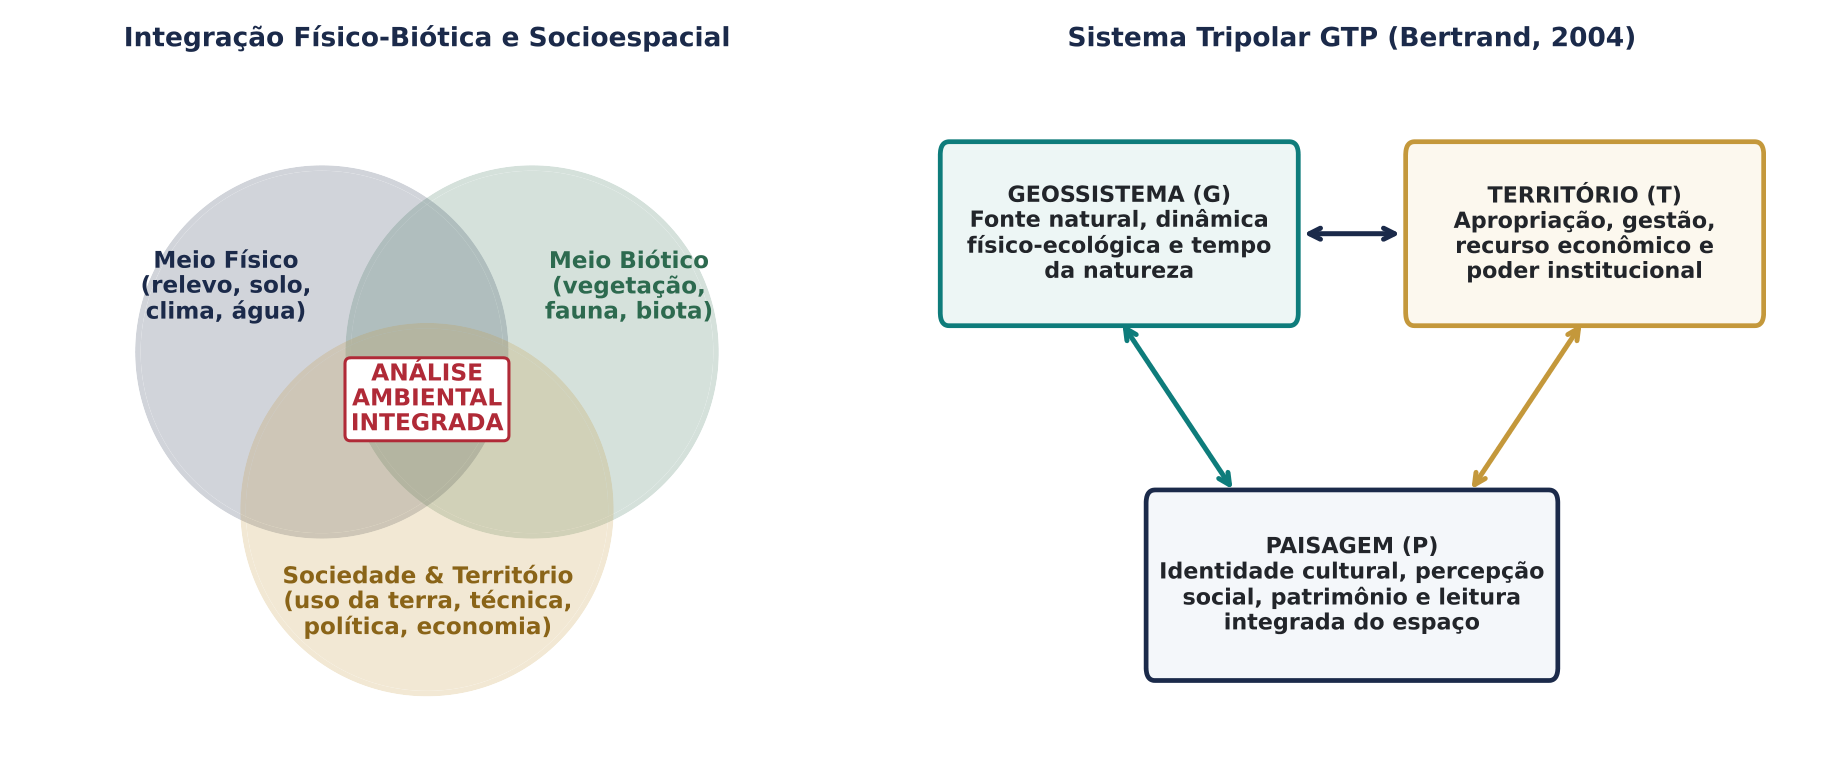
\includegraphics[keepaspectratio]{capitulos/../img/fig01_triade_socioambiental.png}}

}

\caption{\label{fig-triade-gtp}Fundamentos integradores da Análise
Ambiental na Geografia moderna. \textbf{Painel esquerdo.} Articulação
entre Meio Físico, Meio Biótico e Sociedade \& Território, cujo núcleo
de interseção define a Análise Ambiental Integrada sob a perspectiva da
Geografia Socioambiental (Mendonça, 2001). \textbf{Painel direito,}
Sistema Tripolar GTP de Georges Bertrand (2004), evidenciando as
relações bidirecionais entre Geossistema (G), Território (T) e Paisagem
(P) como três entradas complementares sobre a mesma realidade
socioambiental.}

\end{figure}%

Conforme ilustrado na Figura~\ref{fig-triade-gtp}, o Sistema GTP não
divide a realidade em três pedaços independentes; ele estabelece
\textbf{três entradas metodológicas articuladas} para analisar o mesmo
objeto socioambiental em tempos distintos,

\textbf{Polo G, Geossistema (a \emph{fonte} / \emph{source}),} analisa o
funcionamento biofísico e ecológico do espaço, incorporando a
antropização como fator atuante nos fluxos de energia, água, sedimentos
e nutrientes. Opera principalmente no \emph{tempo da natureza} (ciclos
hidrológicos, pedogênese, morfogênese, sucessão ecológica). Responde à
questão, \emph{como o sistema biofísico funciona, responde a
perturbações e sustenta processos ecológicos?} \textbf{Polo T,
Território (o \emph{recurso} / \emph{ressource}),} analisa a dimensão
socioeconômica, jurídica e política. Trata dos modos de apropriação, uso
produtivo da terra, regulação legal, gestão de bacias, distribuição
desigual de benefícios e danos ambientais. Opera no \emph{tempo social e
institucional} (ciclos econômicos, mandatos políticos, prazos de
licenciamento). Responde à questão, \emph{quem apropria, gere, normatiza
e disputa os recursos naturais?}

\textbf{Polo P, Paisagem (a \emph{ressurgência} / identidade e
patrimônio / \emph{ressourcement}),} analisa a dimensão cultural,
simbólica, estética e perceptiva. Investiga como diferentes grupos
sociais percebem, nomeiam, valorizam e atribuem sentido patrimonial ao
ambiente em que vivem. Opera no \emph{tempo da memória e da cultura}.
Responde à questão, \emph{como a sociedade vivencia, representa e
atribui valor identitário a esse espaço?}

O grande ganho do sistema GTP reside nas \textbf{setas bidirecionais}
que conectam os três polos (Figura~\ref{fig-triade-gtp}). Uma alteração
no Território (por exemplo, mudança no plano diretor municipal
permitindo impermeabilização de cabeceiras) altera imediatamente o
Geossistema (aumentando o escoamento superficial e o pico de cheia) e
transforma a Paisagem (substituindo brejos e lagoas por canais
concretados e gerando perda de memória hídrica local). Por sua vez, a
mobilização cultural pela preservação de uma paisagem patrimonial (polo
P) pode induzir a criação de uma Unidade de Conservação (polo T), que
protege a cobertura vegetal e estabiliza o balanço hídrico (polo G).

\subsection{\texorpdfstring{Índice Didático de Equilíbrio Analítico GTP
(\(I_{\text{GTP}}\)), Auditoria de
Diagnósticos}{Índice Didático de Equilíbrio Analítico GTP (I\_\{\textbackslash text\{GTP\}\}), Auditoria de Diagnósticos}}\label{uxedndice-diduxe1tico-de-equiluxedbrio-analuxedtico-gtp-i_textgtp-auditoria-de-diagnuxf3sticos}

Para auditar se um relatório ou diagnóstico ambiental realmente integra
os três polos de Bertrand (2004), em vez de hipertrofiar apenas o meio
físico ou apenas a descrição social, adotamos em CHF662 uma métrica
operacional didática baseada na \textbf{média harmônica} das notas de
cobertura técnica de cada polo (\(g, t, p \in [0, 10]\)),

\[
I_{\text{GTP}} = \frac{3\,g\,t\,p}{g\,t + g\,p + t\,p} \qquad (\text{para } g, t, p > 0)
\]

Caso qualquer um dos três polos esteja completamente ausente (\(g = 0\),
\(t = 0\) ou \(p = 0\)), define-se \(I_{\text{GTP}} = 0\), indicando
ruptura da integração tripolar.

\textbf{Por que usar média harmônica em vez de média aritmética
(\(\text{MA} = \frac{g+t+p}{3}\))?} A média aritmética permite
compensação indevida, um relatório puramente naturalista pode tirar nota
máxima em Geossistema e disfarçar a negligência em Território e
Paisagem. Já a média harmônica penaliza fortemente o polo deficitário,
refletindo o princípio sistêmico de que a integração é limitada pelo elo
mais fraco.

\textbf{Critério didático de classificação em CHF662,}

\(I_{\text{GTP}} \ge 7,0\), diagnóstico socioambiental bem integrado nos
três polos. \(4,0 \le I_{\text{GTP}} < 7,0\), integração parcial (há
polo subdesenvolvido que demanda reforço). \(I_{\text{GTP}} < 4,0\),
diagnóstico fragmentado ou dicotômico (predomínio unilateral de um único
polo).

\textbf{Exemplo numérico comparativo (passo a passo),} Compare dois
relatórios técnicos avaliados na escala de \(0\) a \(10\),

Média aritmética,
\(\text{MA}_A = \frac{9,0 + 2,0 + 1,0}{3} = \frac{12,0}{3} = 4,00\)
(aparentaria integração parcial). Produto dos três polos,
\(g \cdot t \cdot p = 9,0 \times 2,0 \times 1,0 = 18,0\). Numerador,
\(3 \times 18,0 = 54,0\). Denominador,
\((9,0 \times 2,0) + (9,0 \times 1,0) + (2,0 \times 1,0) = 18,0 + 9,0 + 2,0 = 29,0\).
Resultado, \(I_{\text{GTP}, A} = \frac{54,0}{29,0} \approx 1,86\)
(\textbf{fragmentado/dicotômico}).

Média aritmética,
\(\text{MA}_B = \frac{8,0 + 7,5 + 6,0}{3} = \frac{21,5}{3} \approx 7,17\).
Produto dos três polos, \(8,0 \times 7,5 \times 6,0 = 360,0\).
Numerador, \(3 \times 360,0 = 1080,0\). Denominador,
\((8,0 \times 7,5) + (8,0 \times 6,0) + (7,5 \times 6,0) = 60,0 + 48,0 + 45,0 = 153,0\).
Resultado,
\(I_{\text{GTP}, B} = \frac{1080,0}{153,0} = \frac{120}{17} \approx 7,06\)
(\textbf{bem integrado}).

\textbf{Relatório A (viés naturalista),} \(g = 9,0\), \(t = 2,0\),
\(p = 1,0\). \textbf{Relatório B (abordagem integrada),} \(g = 8,0\),
\(t = 7,5\), \(p = 6,0\).

\subsection{Interdisciplinaridade e Análise Ambiental
Integrada}\label{interdisciplinaridade-e-anuxe1lise-ambiental-integrada}

Nenhuma disciplina isolada domina todos os métodos exigidos por um
diagnóstico ambiental de alta complexidade. Entretanto, reunir diversos
profissionais em uma mesma equipe não garante automaticamente uma
análise integrada. A epistemologia ambiental distingue três níveis de
cooperação entre saberes,

\textbf{Multidisciplinaridade (justaposição).} Vários especialistas
(geólogo, biólogo, engenheiro, sociólogo, geógrafo) elaboram capítulos
separados sobre a mesma área, sem formular perguntas comuns nem cruzar
variáveis. O resultado típico é o chamado ``relatório em gavetas'', no
qual o capítulo de solos não dialoga com o de uso da terra nem com o de
saúde pública. \textbf{Interdisciplinaridade (integração metodológica).}
Diferentes disciplinas definem conjuntamente o problema ambiental,
compatibilizam escalas espaciais e temporais, trocam dados e constroem
sínteses integradas (como mapas de fragilidade socioambiental, matrizes
de impacto cruzado e zoneamentos participativos).

\textbf{Transdisciplinaridade (diálogo com saberes não acadêmicos).}
Além de integrar disciplinas científicas, incorpora o conhecimento
empírico e territorial das comunidades locais (agricultores familiares,
pescadores, comunidades de fundo de pasto, quilombolas), fundamental
para compreender o regime histórico de riachos intermitentes, manchas de
solo fértil e usos tradicionais da biota.

Nesse arranjo, qual é a contribuição específica do \textbf{geógrafo}?
Pela formação voltada à espacialidade, à cartografia temática, às
escalas e à interface natureza-sociedade, o geógrafo atua como um
\emph{articulador espacial}, capaz de traduzir dados setoriais
(geológicos, hidrológicos, ecológicos e demográficos) em uma leitura
territorial integrada e propositiva.

\subsection{Integração do GTP e limites da síntese
numérica}\label{integrauxe7uxe3o-do-gtp-e-limites-da-suxedntese-numuxe9rica}

Em um parque eólico, o geossistema permite examinar a circulação da
água, a cobertura vegetal e a estabilidade dos materiais. O território
orienta a análise dos arrendamentos, das regras de circulação e das
competências institucionais. A paisagem permite compreender como os
moradores reconhecem as serras, as alterações visuais e as mudanças no
ambiente sonoro. A integração ocorre quando uma decisão territorial é
relacionada a uma alteração do sistema e à experiência dos grupos
afetados.

O índice didático de equilíbrio GTP utilizado nos exercícios corresponde
a uma média harmônica de notas. Seu valor informa o equilíbrio entre
pontuações atribuídas com uma rubrica explícita. O resultado depende dos
critérios, da escala de notas e da consistência da avaliação. A
atribuição de valores semelhantes aos três polos pode representar
avaliações igualmente superficiais, razão pela qual o número precisa ser
acompanhado das evidências que sustentam cada nota.

Esse índice foi construído para o treinamento proposto na apostila e
deve ser identificado como recurso didático. Ele não constitui um índice
originalmente formulado por Bertrand nem demonstra, isoladamente,
integração científica ou qualidade de um relatório. Uma aplicação
responsável apresenta os critérios de avaliação, compara as
justificativas e informa como mudanças nas notas alteram o resultado.

\section{Etapa 4 - Exemplos
resolvidos}\label{etapa-4---exemplos-resolvidos-2}

\subsection{Exemplo 3.1 - Superando a Dicotomia Físico-Humana em
Enchentes Urbanas
(Básico)}\label{03-geografia-socioambiental-gtp-exemplo-3.1.-superando-a-dicotomia-fuxedsicohumana-em-enchentes-urbanas-buxe1sico}

\textbf{Situação analisada.} Durante a estação chuvosa, bairros situados
na cabeceira do Rio Subaé, em Feira de Santana (BA), sofrem alagamentos
recorrentes. Dois consultores emitiram pareceres conflitantes, o Parecer
1 afirmou que o problema decorre exclusivamente de chuvas convectivas
intensas e relevo plano mal drenado; o Parecer 2 sustentou que se trata
apenas de segregação urbana e descaso político, sem considerar a
hidrografia local. Reformule o diagnóstico sob a ótica da Geografia
Socioambiental.

\textbf{Dados disponíveis.} Local, cabeceira urbana do Rio Subaé (Feira
de Santana, BA). Parecer 1, foco exclusivo em pluviosidade e topografia.
Parecer 2, foco exclusivo em segregação urbana e gestão municipal.
Referencial, Mendonça (2001).

\textbf{Problema a resolver.} Identificar o viés epistemológico presente
em cada parecer e propor uma formulação integrada que supere a
dicotomia.

\textbf{Fundamento da análise.} Análise epistemológica pela Geografia
Socioambiental (Mendonça, 2001), verificando como processos
físico-hidrológicos e decisões socioespaciais se codeterminam.

\textbf{Desenvolvimento.} \textbf{Passo 1, Diagnóstico do Parecer 1.}
Reproduz o reducionismo naturalista (Geografia Física isolada). Ao
atribuir o alagamento apenas à chuva e ao relevo plano, naturaliza um
evento que foi amplificado pela impermeabilização do solo, pelo
aterramento de nascentes/lagoas e pela ocupação de planícies de
inundação.\\
\textbf{Passo 2, Diagnóstico do Parecer 2.} Reproduz o reducionismo
sociologizante (Geografia Humana sem base material). Embora aponte
corretamente a desigualdade urbana, ignora parâmetros físicos
indispensáveis (capacidade de infiltração, cota de inundação, seção de
escoamento), impedindo o dimensionamento de soluções drenantes.\\
\textbf{Passo 3, Reformulação socioambiental integrada.} Articula os
dois eixos em uma cadeia causal única, a expansão urbana sem
planejamento impermeabilizou áreas de recarga e estreitou canais
naturais (processo social/territorial), o que reduziu a infiltração e
elevou o escoamento superficial em eventos de chuva intensa sobre relevo
de baixa declividade (dinâmica físico-hidrológica), atingindo
prioritariamente famílias de menor renda assentadas nas áreas de várzea
(desigualdade socioespacial).

\textbf{Interpretação do resultado.} Ambos os pareceres são dicotômicos
(naturalista no Parecer 1; sociologizante no Parecer 2). A leitura
socioambiental integra a dinâmica hidrológica da cabeceira (infiltração,
relevo plano e chuvas intensas) à produção desigual do espaço urbano
(impermeabilização, aterramento de lagoas e vulnerabilidade
habitacional).

\textbf{Condições de validade.} A síntese faz sentido ambiental e
técnico porque permite combinar ações estruturais (parques lineares,
retenção de águas pluviais, desimpermeabilização) com ações territoriais
e sociais (revisão do zoneamento urbano e regularização fundiária
segura).

\subsection{Exemplo 3.2 - Distinção Operacional entre Espaço, Paisagem,
Território e Ambiente
(Básico)}\label{exemplo-3.2---distinuxe7uxe3o-operacional-entre-espauxe7o-paisagem-territuxf3rio-e-ambiente-buxe1sico}

\textbf{Situação analisada.} Uma equipe de estudantes de CHF662 realiza
trabalho de campo no entorno da Lagoa Grande, em Feira de Santana (BA),
área que passou por obras de urbanização, requalificação paisagística e
controle de drenagem. Em seus cadernos de campo, os alunos registraram
quatro observações distintas e precisam classificá-las corretamente
segundo as quatro categorias geográficas estudadas.

\textbf{Dados disponíveis.} Observação I, ``As margens exibem espelho
d'água cercado por macrófitas, pista de caminhada, vegetação arbustiva e
bairros residenciais, sendo reconhecidas pela população como área de
lazer e memória hídrica da cidade.'' Observação II, ``A fiscalização
municipal e a legislação estadual de APP delimitam faixas não
edificáveis e regulam o uso comercial no entorno.'' Observação III, ``O
aporte de esgoto clandestino elevou a carga de nutrientes na água,
reduzindo o oxigênio dissolvido e alterando a biota aquática.''
Observação IV, ``A requalificação insere a lagoa na rede viária e na
valorização imobiliária da malha urbana de Feira de Santana,
reorganizando objetos técnicos e fluxos da cidade.''

\textbf{Problema a resolver.} Associar cada observação à categoria
geográfica predominante (espaço geográfico, paisagem, território ou
ambiente) e justificar tecnicamente cada enquadramento.

\textbf{Fundamento da análise.} Aplicação dos núcleos analíticos e
perguntas-chave definidos na Seção 3.3 deste capítulo.

\textbf{Desenvolvimento.} \textbf{Passo 1, Observação I.} Enfatiza a
fisionomia visível (espelho d'água, vegetação, pista, bairros) e a
percepção/memória afetiva da população. Corresponde à categoria
\textbf{Paisagem}.\\
\textbf{Passo 2, Observação II.} Enfatiza normas jurídicas (APP),
fiscalização estatal, delimitação de faixas e controle de uso. Trata-se
de relações de poder e gestão, correspondendo à categoria
\textbf{Território}.\\
\textbf{Passo 3, Observação III.} Descreve interações físico-químicas,
bióticas e antrópicas (carga de nutrientes \(\rightarrow\) redução de
oxigênio dissolvido \(\rightarrow\) alteração da biota). Corresponde à
categoria \textbf{Ambiente}.\\
\textbf{Passo 4, Observação IV.} Aborda a totalidade da produção urbana
(integração de sistemas de objetos viários/imobiliários e sistemas de
ações econômicas na cidade). Corresponde à categoria \textbf{Espaço
Geográfico}.

\textbf{Interpretação do resultado.} I = Paisagem; II = Território; III
= Ambiente; IV = Espaço Geográfico.

\textbf{Condições de validade.} Cada categoria respondeu a uma pergunta
diferente sobre o mesmo lugar (Lagoa Grande), comprovando que os quatro
termos não são sinônimos e se complementam na construção do diagnóstico.

\subsection{Exemplo 3.3 - Aplicação do Sistema Tripolar GTP em Parque
Eólico no Semiárido
(Intermediário)}\label{exemplo-3.3---aplicauxe7uxe3o-do-sistema-tripolar-gtp-em-parque-euxf3lico-no-semiuxe1rido-intermediuxe1rio}

\textbf{Situação analisada.} Na preparação para a atividade de campo de
CHF662 no eixo energético do Semiárido Baiano (região de
Canudos/Sertão), solicita-se estruturar um roteiro de análise integrada
sobre a implantação de um complexo eólico em chapadas e tabuleiros de
Caatinga, utilizando o Sistema Tripolar GTP de Georges Bertrand (2004).

\textbf{Dados disponíveis.} Elementos identificados em campo, (a)
abertura de acessos e terraplanagem para bases de aerogeradores em solos
arenosos e pedregosos de Caatinga, com ravinamento incipiente nas bordas
das plataformas; (b) contratos de arrendamento de terras entre empresas
energéticas e proprietários/posseiros, além do licenciamento junto ao
INEMA e disputas por áreas de pastoreio comunitário; (c) transformação
visual das serras sertanejas pelas torres de grande porte, ruído
aerodinâmico e ressignificação do lugar pelos moradores locais.

\textbf{Problema a resolver.} Enquadrar os elementos nos polos G, T e P
e demonstrar duas retroalimentações (interações bidirecionais) entre os
polos.

\textbf{Fundamento da análise.} Matriz tripolar GTP de Bertrand (2004),
Geossistema (fonte/biofísico), Território (recurso/gestão/poder) e
Paisagem (identidade/percepção/patrimônio).

\textbf{Desenvolvimento.} \textbf{Passo 1, Enquadramento no Polo G
(Geossistema).} Refere-se aos elementos (a). Analisa a remoção da
Caatinga, a exposição de solos frágeis ao impacto das chuvas
concentradas do Semiárido, o escoamento concentrado nas estradas de
serviço, a formação de ravinas nas bases das torres e os efeitos sobre a
avifauna local.\\
\textbf{Passo 2, Enquadramento no Polo T (Território).} Refere-se aos
elementos (b). Analisa a governança energética, os contratos de
arrendamento, as condicionantes do licenciamento ambiental (INEMA), a
reorganização fundiária e os conflitos de acesso a áreas tradicionais de
fundo de pasto.\\
\textbf{Passo 3, Enquadramento no Polo P (Paisagem).} Refere-se aos
elementos (c). Analisa a alteração da fisionomia das serras, a percepção
sonora e visual do parque pelos moradores e o conflito entre o discurso
da ``energia limpa'' e a memória territorial sertaneja.\\
\textbf{Passo 4, Interações bidirecionais,}

\(T \leftrightarrow G\), decisões contratuais e de traçado viário do
empreendimento (\(T\)) determinam onde ocorrerá supressão vegetal e
terraplanagem, desencadeando erosão em encostas (\(G\)); em sentido
inverso, a erosão que desestabiliza estradas e taludes (\(G\)) impõe
custos de manutenção e obrigações corretivas no licenciamento (\(T\)).
\(P \leftrightarrow T\), a percepção negativa de ruído e de
descaracterização das serras (\(P\)) fortalece a mobilização comunitária
por audiências públicas e revisão de distâncias mínimas das torres em
relação às casas (\(T\)).

\textbf{Interpretação do resultado.} Polo G, dinâmica
solo-água-vegetação-avifauna nas plataformas e acessos; Polo T,
arrendamentos, licenciamento e conflitos fundiários; Polo P,
reconfiguração visual/sonora e identidade sertaneja. As conexões
\(T \leftrightarrow G\) e \(P \leftrightarrow T\) demonstram a
indivisibilidade do sistema.

\textbf{Condições de validade.} O roteiro cobre todas as dimensões
exigidas na viagem de campo da Semana 11, evitando reduzir a energia
eólica a um debate exclusivamente técnico-elétrico ou exclusivamente
paisagístico.

\subsection{\texorpdfstring{Exemplo 3.4 - Auditoria Quantitativa de
Relatórios Ambientais com o Índice \(I_{\text{GTP}}\)
(Intermediário)}{Exemplo 3.4 - Auditoria Quantitativa de Relatórios Ambientais com o Índice I\_\{\textbackslash text\{GTP\}\} (Intermediário)}}\label{exemplo-3.4---auditoria-quantitativa-de-relatuxf3rios-ambientais-com-o-uxedndice-i_textgtp-intermediuxe1rio}

\textbf{Situação analisada.} Para subsidiar o plano de gestão de uma
microbacia no Vale do Paraguaçu (BA), um órgão público avaliou dois
diagnósticos preliminares elaborados por consultorias diferentes. A
comissão avaliadora atribuiu notas de \(0\) a \(10\) para a consistência
técnica em cada polo do sistema GTP. Verifique numericamente qual
diagnóstico apresenta real integração socioambiental.

\textbf{Dados disponíveis.} Diagnóstico X, Geossistema \(g_X = 10,0\);
Território \(t_X = 1,0\); Paisagem \(p_X = 1,0\). Diagnóstico Y,
Geossistema \(g_Y = 4,0\); Território \(t_Y = 4,0\); Paisagem
\(p_Y = 4,0\). Critério de referência,
\(I_{\text{GTP}} = \frac{3\,g\,t\,p}{g\,t + g\,p + t\,p}\).

\textbf{Problema a resolver.} Calcular a média aritmética
(\(\text{MA}\)) e o índice \(I_{\text{GTP}}\) de ambos os diagnósticos e
interpretar o significado metodológico da diferença encontrada.

\textbf{Fundamento da análise.} Cálculo passo a passo de \(\text{MA}\) e
\(I_{\text{GTP}}\) conforme o quadro de fórmulas da Etapa 3.

\textbf{Desenvolvimento.} \textbf{Passo 1, Médias aritméticas,}

\[
\text{MA}_X = \frac{10{,}0 + 1{,}0 + 1{,}0}{3} = \frac{12{,}0}{3} = 4{,}00 \qquad\text{e}\qquad \text{MA}_Y = \frac{4{,}0 + 4{,}0 + 4{,}0}{3} = \frac{12{,}0}{3} = 4{,}00.
\]

Pela média aritmética simples, os dois relatórios pareceriam
empatados!\\
\textbf{Passo 2, Cálculo de \(I_{\text{GTP}}\) para o Diagnóstico X,}

Numerador,
\(3 \times g_X \times t_X \times p_X = 3 \times 10,0 \times 1,0 \times 1,0 = 30,0\).
Denominador,
\((10,0 \times 1,0) + (10,0 \times 1,0) + (1,0 \times 1,0) = 10,0 + 10,0 + 1,0 = 21,0\).
Quociente,
\(I_{\text{GTP}, X} = \frac{30,0}{21,0} = \frac{10}{7} \approx 1,43\)
(diagnóstico fragmentado/dicotômico).

\textbf{Passo 3, Cálculo de \(I_{\text{GTP}}\) para o Diagnóstico Y,}

Numerador, \(3 \times 4,0 \times 4,0 \times 4,0 = 192,0\). Denominador,
\((4,0 \times 4,0) + (4,0 \times 4,0) + (4,0 \times 4,0) = 16,0 + 16,0 + 16,0 = 48,0\).
Quociente, \(I_{\text{GTP}, Y} = \frac{192,0}{48,0} = 4,00\) (integração
parcial, porém equilibrada).

\textbf{Passo 4, Comparação percentual.} O Diagnóstico Y obtém
\(I_{\text{GTP}}\) superior ao de X em
\(\frac{4,00 - 1,43}{1,43} \times 100\% \approx 180\%\), apesar da mesma
soma de notas (\(12,0\)).

\textbf{Interpretação do resultado.}
\(\text{MA}_X = \text{MA}_Y = 4,00\); contudo,
\(I_{\text{GTP}, X} \approx 1,43\) (fragmentado) e
\(I_{\text{GTP}, Y} = 4,00\) (integração parcial equilibrada). O
Diagnóstico Y é mais coerente com a abordagem socioambiental, embora
ambos precisem ser aprimorados para atingir o patamar integrado
(\(\ge 7,0\)).

\textbf{Condições de validade.} O resultado faz pleno sentido matemático
(pela desigualdade entre médias, a média harmônica é sempre menor ou
igual à média aritmética, igualando-se apenas quando \(g = t = p\)) e
ambiental (excelência isolada em mapeamento físico não compensa a
omissão de conflitos territoriais e da percepção social).

\subsection{Exemplo 3.5 - Desenho de Projeto Interdisciplinar em
Microbacia Periurbana
(Avançado)}\label{exemplo-3.5---desenho-de-projeto-interdisciplinar-em-microbacia-periurbana-avanuxe7ado}

\textbf{Situação analisada.} A prefeitura de um município da Região
Metropolitana de Feira de Santana contratou um estudo ambiental para uma
microbacia afluente do Rio Jacuípe que enfrenta desmatamento de mata
ciliar, retirada irregular de areia e expansão de chácaras sem
esgotamento sanitário. A proposta inicial da empresa previa cinco
relatórios isolados (Geologia, Botânica, Hidrologia, Economia e
Sociologia) entregues em anexos separados, em escalas cartográficas
diferentes (\(1:100.000\) na Geologia e \(1:5.000\) no cadastro urbano).
Reestruture a proposta para garantir interdisciplinaridade efetiva.

\textbf{Dados disponíveis.} Área, microbacia periurbana afluente do Rio
Jacuípe (BA). Problemas, supressão ripária, mineração irregular de
areia, loteamento sem saneamento. Proposta inicial, 5 anexos
independentes com escalas incompatíveis (\(1:100.000\) vs.~\(1:5.000\)).

\textbf{Problema a resolver.} Diagnosticar a falha metodológica da
proposta original e propor um protocolo interdisciplinar e
transdisciplinar de trabalho.

\textbf{Fundamento da análise.} Distinção entre multidisciplinaridade,
interdisciplinaridade e transdisciplinaridade articulada ao papel
integrador do geógrafo e à compatibilização de escalas.

\textbf{Desenvolvimento.} \textbf{Passo 1, Diagnóstico da falha.} A
proposta original caracteriza \textbf{multidisciplinaridade justaposta}.
Além de não formular um problema comum, a incompatibilidade escalar
impede o cruzamento espacial, uma base geológica \(1:100.000\) não
permite localizar processos erosivos de margem nem relacioná-los aos
lotes em escala \(1:5.000\).\\
\textbf{Passo 2, Recorte espacial e escala comum.} Adotar a
\textbf{microbacia hidrográfica} como unidade física de integração,
harmonizando todas as camadas temáticas (solos, declividade, cobertura
vegetal, uso da terra, pontos de lançamento de efluentes e cavas de
areia) na escala operacional de detalhe (\(1:10.000\) ou \(1:5.000\)).\\
\textbf{Passo 3, Pergunta interdisciplinar unificadora.} Substituir os
cinco inventários soltos por uma questão articuladora, \emph{como a
expansão de chácaras e a extração de areia alteram a conectividade
hidrossedimentológica, a qualidade da água e os conflitos territoriais
na microbacia?}\\
\textbf{Passo 4, Produtos integrados e transdisciplinaridade.} Gerar um
mapa-síntese socioambiental (cruzando polos G, T e P) e realizar
oficinas participativas com moradores e pequenos produtores para
incorporar o histórico local de cheias, nascentes extintas e usos
tradicionais da água (dimensão transdisciplinar).

\textbf{Interpretação do resultado.} A proposta original é meramente
multidisciplinar e escalarmente incompatível. A reestruturação exige
unidade espacial comum (microbacia em escala de detalhe
\(1:5.000\)-\(1:10.000\)), pergunta-problema compartilhada, matriz
integradora GTP e oficinas participativas (transdisciplinaridade).

\textbf{Condições de validade.} A solução assegura que os dados físicos
(erosão e qualidade hídrica) orientem diretamente o ordenamento
territorial e a fiscalização ambiental, evitando relatórios desconexos
que nunca saem da gaveta.

\section{Etapa 5 - Erros de
interpretação}\label{etapa-5---erros-de-interpretauxe7uxe3o-2}

\subsection{Erro 1, Empregar Espaço, Paisagem, Território e Ambiente
como
Sinônimos}\label{erro-1-empregar-espauxe7o-paisagem-territuxf3rio-e-ambiente-como-sinuxf4nimos}

\textbf{Equívoco frequente.} Em textos acadêmicos e relatórios, o
estudante escreve ``território'' em um parágrafo e ``paisagem'' ou
``ambiente'' no parágrafo seguinte apenas para evitar repetir a mesma
palavra.\\
\textbf{Por que está incorreto.} Cada categoria define um recorte
teórico e operacional distinto. Falar em ``preservar a paisagem'' quando
o conflito envolve disputa fundiária ou poder de gestão (território)
enfraquece a precisão técnica do argumento.\\
\textbf{Como evitar.} Antes de escolher o termo, pergunte qual é o foco
da frase, se for poder/gestão/norma, use \emph{território}; se for
fisionomia/memória/percepção, use \emph{paisagem}; se for interação
físico-biótico-social, use \emph{ambiente}; se for totalidade de objetos
e ações, use \emph{espaço geográfico}.

\subsection{Erro 2, Confundir Geografia Socioambiental com Soma Mecânica
de
Capítulos}\label{erro-2-confundir-geografia-socioambiental-com-soma-mecuxe2nica-de-capuxedtulos}

\textbf{Equívoco frequente.} Acreditar que basta escrever uma seção de
``aspectos físicos'' (clima, relevo, solo) e outra seção separada de
``aspectos humanos'' (população, economia) para cumprir a abordagem
socioambiental de Mendonça (2001).\\
\textbf{Por que está incorreto.} Justapor partes desconexas reproduz a
dicotomia clássico-positivista sob aparência integrada
(multidisciplinaridade fragmentada).\\
\textbf{Como evitar.} Explicite sempre as \textbf{relações causais e de
retroalimentação} entre as dinâmicas naturais e sociais (por exemplo,
como o modelo de manejo do solo intensifica a erosão e como essa erosão
reduz a renda agrícola e agrava conflitos locais).

\subsection{Erro 3, Entender o Polo Geossistema (G) como ``Natureza
Intocada''}\label{erro-3-entender-o-polo-geossistema-g-como-natureza-intocada}

\textbf{Equívoco frequente.} Imaginar que, no Sistema GTP de Bertrand
(2004), o Geossistema exclui qualquer ação humana e só existiria em
florestas virgens ou parques sem moradores.\\
\textbf{Por que está incorreto.} Desde 1968, e de forma ainda mais clara
no modelo GTP, Bertrand inclui a \textbf{antropização} como componente
interno da dinâmica geossistêmica. Uma bacia rural cultivada ou uma
várzea urbana continuam operando como geossistemas, agora profundamente
modificados pela sociedade.\\
\textbf{Como evitar.} Lembre que o polo G focaliza o \emph{funcionamento
biofísico e ecológico} (incluindo os efeitos físicos da ação humana),
enquanto os polos T e P tratam da gestão/poder e da
identidade/percepção.

\subsection{Erro 4, Tratar a Paisagem (P) como Aspecto Meramente
Decorativo ou
Estético}\label{erro-4-tratar-a-paisagem-p-como-aspecto-meramente-decorativo-ou-estuxe9tico}

\textbf{Equívoco frequente.} Desvalorizar o polo Paisagem do sistema GTP
em diagnósticos ambientais, considerando-o ``subjetivo demais'' frente
aos dados numéricos de solo e água.\\
\textbf{Por que está incorreto.} A paisagem expressa vínculos de
pertencimento, memória coletiva e leitura histórica do espaço. Projetos
de intervenção (como barragens, parques eólicos ou recuperação de lagoas
urbanas) frequentemente fracassam ou geram forte resistência social
quando ignoram o valor identitário e patrimonial que as comunidades
atribuem à paisagem.\\
\textbf{Como evitar.} Integre levantamentos de percepção ambiental,
história oral e patrimônio paisagístico ao diagnóstico físico e
territorial.

\section{Etapa 6 - Exercícios de
fixação}\label{etapa-6---exercuxedcios-de-fixauxe7uxe3o-2}

\subsubsection{Nível Básico (Exercícios 1 a
5)}\label{nuxedvel-buxe1sico-exercuxedcios-1-a-5}

\begin{enumerate}
\def\labelenumi{\arabic{enumi}.}
\item
  Explique, com suas próprias palavras, qual é a principal diferença
  entre a visão da relação sociedade-natureza no \textbf{determinismo
  ambiental} e no \textbf{possibilismo}.
\item
  Por que a Geografia Crítica das décadas de 1970 e 1980, apesar de seus
  avanços na compreensão da produção social do espaço, acabou reforçando
  indiretamente a dicotomia entre Geografia Física e Geografia Humana?
\item
  Segundo Mendonça (2001), por que a expressão \textbf{Geografia
  Socioambiental} utiliza o prefixo ``socio''? Isso representa uma
  redundância conceitual? Justifique.
\item
  Indique os três polos do \textbf{Sistema Tripolar GTP} proposto por
  Georges Bertrand (2004), associando cada polo ao seu papel analítico
  principal (\emph{fonte}, \emph{recurso} ou
  \emph{identidade/patrimônio}).
\item
  Diferencie \textbf{multidisciplinaridade} de
  \textbf{interdisciplinaridade} na elaboração de um diagnóstico
  ambiental de bacia hidrográfica.
\end{enumerate}

\subsubsection{Nível Intermediário (Exercícios 6 a
10)}\label{nuxedvel-intermediuxe1rio-exercuxedcios-6-a-10}

\begin{enumerate}
\def\labelenumi{\arabic{enumi}.}
\setcounter{enumi}{5}
\item
  Observe a Figura~\ref{fig-triade-gtp} (Painel direito). Por que as
  setas que conectam Geossistema (G), Território (T) e Paisagem (P) são
  \textbf{bidirecionais} (\(\leftrightarrow\)) e não unidirecionais
  (\(\rightarrow\))? Dê um exemplo concreto no Semiárido baiano.
\item
  Em um município do Recôncavo Baiano, a expansão de loteamentos sobre
  áreas de manguezal provocou supressão vegetal, assoreamento de canais
  de maré, disputa judicial com marisqueiras e perda de referência
  cultural da comunidade pesqueira. Classifique esses quatro fenômenos
  segundo as categorias \textbf{ambiente}, \textbf{território} e
  \textbf{paisagem}, indicando como eles se articulam no \textbf{espaço
  geográfico}.
\item
  Dois grupos de estudantes apresentaram propostas de Diagnóstico
  Ambiental para uma microbacia de Feira de Santana (BA) e receberam as
  seguintes notas nos polos GTP,

  \begin{itemize}
  \item
    \textbf{Grupo 1,} \(g = 10,0\); \(t = 2,0\); \(p = 2,0\).
  \item
    \textbf{Grupo 2,} \(g = 6,0\); \(t = 6,0\); \(p = 6,0\).
  \end{itemize}

  Calcule a média aritmética (\(\text{MA}\)) e o índice de equilíbrio
  \(I_{\text{GTP}}\) de cada grupo, passo a passo, e classifique o nível
  de integração de ambos os trabalhos.
\item
  Um parecer técnico sobre desertificação no norte da Bahia descreve
  detalhadamente o déficit hídrico climático e o sobrepastejo caprino,
  mas omite completamente a estrutura fundiária, a ausência de
  assistência técnica rural e o modo como os sertanejos percebem o
  ressecamento das nascentes. Analise criticamente esse parecer à luz do
  Sistema GTP.
\item
  Explique como a \textbf{transdisciplinaridade} pode enriquecer um
  diagnóstico ambiental conduzido por geógrafos em comunidades rurais de
  fundo de pasto no Semiárido baiano, citando dois tipos de informações
  locais que raramente constam em bases cartográficas oficiais.
\end{enumerate}

\subsubsection{Nível Aplicado, Questões Objetivas (Exercícios 11 a
15)}\label{nuxedvel-aplicado-questuxf5es-objetivas-exercuxedcios-11-a-15}

\begin{enumerate}
\def\labelenumi{\arabic{enumi}.}
\setcounter{enumi}{10}
\item
  Em relação à evolução das abordagens ambientais no pensamento
  geográfico moderno, assinale a alternativa correta,

  \begin{enumerate}
  \def\labelenumii{(\Alph{enumii})}
  \item
    A Geografia Clássica do século XIX recusava qualquer estudo sobre
    clima, relevo ou vegetação, concentrando-se apenas na economia
    urbana.
  \item
    O determinismo ambiental defendia que a técnica humana supera
    integralmente os limites ecológicos de qualquer região.
  \item
    A Geografia Socioambiental (Mendonça, 2001) propõe superar a
    separação entre Geografia Física e Geografia Humana integrando
    processos naturais e dinâmicas sociais.
  \item
    A Geografia Teorético-Quantitativa eliminou o uso de modelos
    sistêmicos por considerá-los incompatíveis com a análise ambiental.
  \item
    A Geografia Crítica dos anos 1970 priorizou o estudo da pedogênese e
    da geomorfologia de vertentes como eixo central de suas pesquisas.
  \end{enumerate}
\item
  No planejamento de uma Unidade de Conservação na Chapada Diamantina
  (BA), o analista precisa examinar as normas de uso do solo, o
  zoneamento do plano de manejo e os conflitos de competência entre
  órgãos municipais, estaduais e associações comunitárias. A categoria
  geográfica que expressa diretamente essa dimensão de poder e gestão é,

  \begin{enumerate}
  \def\labelenumii{(\Alph{enumii})}
  \item
    Geótopo.
  \item
    Território.
  \item
    Potencial ecológico.
  \item
    Bioma.
  \item
    Clímax edáfico.
  \end{enumerate}
\item
  No Sistema Tripolar GTP de Georges Bertrand (2004), a correspondência
  correta entre os polos e seus respectivos focos analíticos é,

  \begin{enumerate}
  \def\labelenumii{(\Alph{enumii})}
  \item
    Geossistema = identidade cultural; Território = fluxos hidrológicos;
    Paisagem = normas jurídicas.
  \item
    Geossistema = recurso econômico; Território = tempo geológico;
    Paisagem = apenas estética de cartões-postais.
  \item
    Geossistema = natureza intocada sem ação humana; Território = clima
    regional; Paisagem = bacia hidrográfica.
  \item
    Geossistema = funcionamento biofísico e ecológico (fonte);
    Território = apropriação, gestão e poder (recurso); Paisagem =
    percepção, identidade e patrimônio (ressurgência).
  \item
    Geossistema = modelo matemático urbano; Território = vegetação
    nativa; Paisagem = levantamento topográfico sem observador.
  \end{enumerate}
\item
  Um Estudo de Impacto Ambiental (EIA) reúne capítulos elaborados
  isoladamente por um geólogo, um biólogo e um sociólogo, sem cruzamento
  cartográfico, sem padronização de escala e sem discussão conjunta das
  causas dos impactos. Epistemologicamente, esse estudo caracteriza-se
  como,

  \begin{enumerate}
  \def\labelenumii{(\Alph{enumii})}
  \item
    Transdisciplinar, pois envolve especialistas de diferentes áreas
    técnicas.
  \item
    Interdisciplinar, uma vez que contém tanto dados naturais quanto
    sociais no mesmo volume.
  \item
    Multidisciplinar justaposto, pois soma descrições setoriais sem
    integração metodológica real.
  \item
    Sistêmico tripolar, por apresentar exatamente três profissionais na
    equipe técnica.
  \item
    Possibilista integrado, por respeitar a autonomia absoluta de cada
    disciplina.
  \end{enumerate}
\item
  Um relatório de diagnóstico ambiental obteve notas \(g = 8,0\) em
  Geossistema, \(t = 8,0\) em Território e \(p = 0,0\) em Paisagem
  (ausência total de análise paisagística e perceptiva). Aplicando o
  critério didático do índice \(I_{\text{GTP}}\), conclui-se que,

  \begin{enumerate}
  \def\labelenumii{(\Alph{enumii})}
  \item
    O relatório alcança integração plena, pois a média aritmética dos
    dois polos preenchidos é \(8,0\).
  \item
    \(I_{\text{GTP}} = 0,0\), evidenciando ruptura da integração
    tripolar pela supressão completa do polo Paisagem.
  \item
    \(I_{\text{GTP}} = 5,33\), classificando o relatório como
    parcialmente integrado.
  \item
    A ausência do polo Paisagem é irrelevante em diagnósticos
    ambientais, pois o polo P não interfere na gestão territorial.
  \item
    O relatório deve ser considerado de viés exclusivamente
    sociologizante.
  \end{enumerate}
\end{enumerate}

\section{Etapa 7 - Questões de
aplicação}\label{etapa-7---questuxf5es-de-aplicauxe7uxe3o-2}

\subsection{Estratégia para o Estudo Orientado 2 (EO2) e para a
Avaliação
Teórica}\label{estratuxe9gia-para-o-estudo-orientado-2-eo2-e-para-a-avaliauxe7uxe3o-teuxf3rica}

No \textbf{EO2} (Semana 3, baseado em Mendonça, 2001, e Bertrand, 2004)
e na \textbf{Prova Teórica} (Semana 10), as questões dissertativas e
objetivas costumam cobrar três habilidades integradas,

\begin{enumerate}
\def\labelenumi{\arabic{enumi}.}
\item
  Demonstrar por que a análise ambiental não se reduz à Geografia Física
  isolada nem à Geografia Humana desconectada da base biofísica.
\item
  Aplicar corretamente as categorias \emph{espaço, paisagem, território
  e ambiente} a um caso concreto (evitando definições decoradas sem
  exemplo).
\item
  Articular os três polos do \textbf{Sistema GTP} destacando as
  interações entre o tempo da natureza (G), o tempo da gestão/economia
  (T) e o tempo da cultura/memória (P).
\end{enumerate}

\begin{enumerate}
\def\labelenumi{\arabic{enumi}.}
\setcounter{enumi}{15}
\item
  \textbf{(Questão autoral, estilo ENADE / Geografia)} A implantação de
  grandes projetos de irrigação no Vale do São Francisco reorganizou o
  uso da água, substituiu extensas áreas de Caatinga por monocultivos de
  fruticultura, redefiniu relações fundiárias e alterou profundamente o
  modo como populações ribeirinhas vivenciam e representam o rio.
  Analisando essa transformação à luz da Geografia Socioambiental
  (Mendonça, 2001) e do Sistema GTP (Bertrand, 2004), avalie as
  afirmações a seguir,

  \begin{enumerate}
  \def\labelenumii{\Roman{enumii}.}
  \item
    O polo Geossistema (G) permite investigar exclusivamente a vazão
    natural anterior à construção de barragens, devendo excluir os
    efeitos da irrigação sobre a salinização dos solos.
  \item
    O polo Território (T) evidencia a apropriação diferencial dos
    recursos hídricos, o papel das políticas públicas de irrigação e os
    conflitos entre grandes empreendimentos e agricultores familiares.
  \item
    O polo Paisagem (P) capta a reconfiguração fisionômica das margens e
    a transformação simbólica e identitária na relação das comunidades
    ribeirinhas com o rio.
  \item
    A articulação entre G, T e P supera a dicotomia clássico-positivista
    ao demonstrar que impactos hidrológicos e conflitos fundiários
    pertencem à mesma totalidade socioambiental.
  \end{enumerate}

  É correto apenas o que se afirma em,

  \begin{enumerate}
  \def\labelenumii{(\Alph{enumii})}
  \item
    I e II.
  \item
    I e III.
  \item
    II e IV.
  \item
    II, III e IV.
  \item
    I, II, III e IV.
  \end{enumerate}
\item
  \textbf{(Questão autoral, estilo Concurso Analista Ambiental /
  INEMA-IBAMA)} Em uma audiência pública para licenciamento de rodovia
  estadual que atravessa serras e comunidades tradicionais no interior
  da Bahia, a equipe consultora apresentou um relatório contendo mapas
  detalhados de litologia, declividade e remanescentes florestais, mas
  declarou que ``os conflitos fundiários e o valor cultural atribuído às
  serras pelas comunidades locais fogem ao escopo ambiental por serem
  temas estritamente sociológicos''. À luz dos fundamentos da Análise
  Ambiental na Geografia moderna, essa justificativa é,

  \begin{enumerate}
  \def\labelenumii{(\Alph{enumii})}
  \item
    Correta, pois a análise ambiental restringe-se aos meios físico e
    biótico, deixando questões territoriais para o Poder Judiciário.
  \item
    Correta, visto que o conceito de geossistema exclui variáveis
    culturais e institucionais de qualquer estudo de impacto.
  \item
    Incorreta, pois reproduz a dicotomia natureza-sociedade e
    desconsidera que território e paisagem são dimensões constitutivas
    da análise ambiental integrada.
  \item
    Incorreta apenas quanto aos conflitos fundiários, sendo correta
    quanto à exclusão do valor cultural das serras, que não possui
    relevância geográfica.
  \item
    Parcialmente correta, pois a interdisciplinaridade exige que os
    temas sociais sejam analisados somente após a emissão da licença de
    operação.
  \end{enumerate}
\item
  \textbf{(Questão autoral, estilo Concurso Geógrafo / Planejamento
  Territorial)} Assinale a alternativa que estabelece corretamente a
  relação entre \textbf{escala}, \textbf{interdisciplinaridade} e
  \textbf{categorias geográficas} na condução de um diagnóstico
  ambiental aplicado em microbacias hidrográficas,

  \begin{enumerate}
  \def\labelenumii{(\Alph{enumii})}
  \item
    A justaposição de mapas em escalas incompatíveis (\(1:250.000\) e
    \(1:2.000\)) é desejável porque amplia a diversidade de fontes no
    relatório multidisciplinar.
  \item
    O geógrafo substitui integralmente biólogos, engenheiros e juristas
    na análise ambiental, dispensando a cooperação interdisciplinar.
  \item
    A distinção entre espaço, paisagem, território e ambiente é
    irrelevante na prática técnica, servindo apenas para debates
    filosóficos sem repercussão cartográfica.
  \item
    A análise ambiental integrada requer compatibilização de escalas
    espaciais e temporais, formulação interdisciplinar do problema e
    articulação das dinâmicas biofísicas (G) com a gestão territorial
    (T) e a leitura paisagística (P).
  \item
    A transdisciplinaridade consiste em substituir medições de campo e
    dados hidrológicos exclusivamente por relatos informais de moradores
    locais.
  \end{enumerate}
\end{enumerate}

\section{Etapa 8 - Gabarito
comentado}\label{etapa-8---gabarito-comentado-2}

\subsection{Resolução, Nível Básico (Exercícios 1 a
5)}\label{resoluuxe7uxe3o-nuxedvel-buxe1sico-exercuxedcios-1-a-5}

\begin{enumerate}
\def\labelenumi{\arabic{enumi}.}
\item
  \textbf{Determinismo vs.~Possibilismo.} No \emph{determinismo
  ambiental} (associado a Ratzel e leituras deterministas posteriores),
  as condições naturais (clima, relevo, solo) determinam diretamente a
  organização e o desenvolvimento das sociedades. No \emph{possibilismo}
  (Vidal de La Blache), a natureza oferece possibilidades e
  condicionantes, cabendo à sociedade escolher, adaptar-se e transformar
  o meio por intermédio da técnica, da cultura e do \emph{gênero de
  vida}.
\item
  \textbf{Geografia Crítica e dicotomia.} Ao reagir ao formalismo
  quantitativo e priorizar o materialismo histórico e as relações
  sociais de produção, parte expressiva da Geografia Humana crítica dos
  anos 1970 a 1980 afastou-se do estudo dos processos naturais (relevo,
  solos, clima, hidrologia). Em paralelo, setores da Geografia Física
  mantiveram-se restritos a análises naturalistas, consolidando duas
  comunidades científicas com pouco diálogo.
\item
  \textbf{Prefixo ``socio'' em Mendonça (2001).} Não é redundância. Ele
  marca explicitamente o rompimento com a tradição naturalista que
  igualava ``ambiente'' à natureza sem seres humanos. O termo
  \emph{Geografia Socioambiental} afirma que a dinâmica natural e a
  organização social atuam de forma indissociável na produção e na
  resolução dos problemas ambientais.
\item
  \textbf{Sistema Tripolar GTP (Bertrand, 2004),} \textbf{Geossistema
  (G)} = polo naturalista/biofísico, entendido como \emph{fonte}
  (\emph{source}) e dinâmicas ecológicas; \textbf{Território (T)} = polo
  socioeconômico, jurídico e político, entendido como \emph{recurso}
  (\emph{ressource}) e gestão; \textbf{Paisagem (P)} = polo cultural,
  identitário e perceptivo, entendido como
  \emph{patrimônio/ressurgência} (\emph{resourcement}).
\item
  \textbf{Multidisciplinaridade vs.~Interdisciplinaridade.} Na
  \emph{multidisciplinaridade}, especialistas produzem diagnósticos
  paralelos e isolados sobre a mesma bacia (capítulos justapostos sem
  diálogo). Na \emph{interdisciplinaridade}, as áreas definem
  conjuntamente o problema, compatibilizam escalas, cruzam variáveis
  físicas, bióticas e sociais e constroem sínteses integradas.
\end{enumerate}

\subsection{Resolução, Nível Intermediário (Exercícios 6 a
10)}\label{resoluuxe7uxe3o-nuxedvel-intermediuxe1rio-exercuxedcios-6-a-10}

\begin{enumerate}
\def\labelenumi{\arabic{enumi}.}
\setcounter{enumi}{5}
\item
  \textbf{Setas bidirecionais na Figura~\ref{fig-triade-gtp}.} Indicam
  causalidade recíproca (retroalimentação) entre os três polos, sem
  hierarquia rígida de mão única. \emph{Exemplo no Semiárido baiano,} a
  implantação de perímetro irrigado ou parque eólico (decisão de gestão
  no polo T) remove a Caatinga e intensifica processos erosivos ou
  salinização (alteração no polo G), modificando a fisionomia e o
  vínculo comunitário com o lugar (polo P); por sua vez, a perda
  produtiva do solo (G) e a resistência cultural local (P) pressionam a
  revisão de licenças e normas territoriais (T).
\item
  \textbf{Manguezal no Recôncavo Baiano,}

  \begin{itemize}
  \item
    \emph{Ambiente,} supressão vegetal do manguezal e assoreamento dos
    canais de maré (interação físico-biótica alterada por ação
    antrópica).
  \item
    \emph{Território,} expansão de loteamentos sobre área protegida e
    disputa judicial com as marisqueiras pelo controle e acesso ao
    estuário.
  \item
    \emph{Paisagem,} transformação visual do estuário e perda de
    referência cultural/identitária da comunidade pesqueira.
  \item
    \emph{Espaço Geográfico,} totalidade histórica que articula a
    expansão imobiliária, as infraestruturas urbanas, o estuário e as
    ações dos diferentes agentes sociais.
  \end{itemize}
\item
  \textbf{Cálculo passo a passo de \(\text{MA}\) e \(I_{\text{GTP}}\),}

  \begin{itemize}
  \item
    \textbf{Grupo 1 (\(g = 10,0\); \(t = 2,0\); \(p = 2,0\)),}

    \begin{itemize}
    \item
      Média aritmética,
      \(\text{MA}_1 = \frac{10,0 + 2,0 + 2,0}{3} = \frac{14,0}{3} \approx 4,67\).
    \item
      Numerador de \(I_{\text{GTP}}\),
      \(3 \times 10,0 \times 2,0 \times 2,0 = 120,0\).
    \item
      Denominador de \(I_{\text{GTP}}\),
      \((10,0 \times 2,0) + (10,0 \times 2,0) + (2,0 \times 2,0) = 20,0 + 20,0 + 4,0 = 44,0\).
    \item
      Índice,
      \(I_{\text{GTP}, 1} = \frac{120,0}{44,0} = \frac{30}{11} \approx 2,73\)
      (\textbf{fragmentado/dicotômico}, pois \(< 4,0\)).
    \end{itemize}
  \item
    \textbf{Grupo 2 (\(g = 6,0\); \(t = 6,0\); \(p = 6,0\)),}

    \begin{itemize}
    \item
      Média aritmética,
      \(\text{MA}_2 = \frac{6,0 + 6,0 + 6,0}{3} = 6,00\).
    \item
      Numerador de \(I_{\text{GTP}}\),
      \(3 \times 6,0 \times 6,0 \times 6,0 = 648,0\).
    \item
      Denominador de \(I_{\text{GTP}}\),
      \((6,0 \times 6,0) + (6,0 \times 6,0) + (6,0 \times 6,0) = 36,0 + 36,0 + 36,0 = 108,0\).
    \item
      Índice, \(I_{\text{GTP}, 2} = \frac{648,0}{108,0} = 6,00\)
      (\textbf{integração parcial equilibrada}, faixa
      \(4,0 \le I_{\text{GTP}} < 7,0\)).
    \end{itemize}
  \item
    \textbf{Conclusão.} O Grupo 2 alcança integração significativamente
    superior (\(6,00\) vs.~\(2,73\)), demonstrando que o equilíbrio
    entre os três polos supera o desempenho unilateral de um único polo.
  \end{itemize}
\item
  \textbf{Crítica ao parecer sobre desertificação.} O parecer contempla
  parcialmente o polo \textbf{Geossistema (G)} (déficit hídrico e
  sobrepastejo), mas falha severamente nos polos \textbf{Território (T)}
  (ao omitir concentração fundiária, crédito e assistência técnica que
  condicionam a lotação animal) e \textbf{Paisagem (P)} (ao
  desconsiderar a percepção e a memória hídrica dos sertanejos). Por
  isso, gera recomendações técnicas limitadas ou culpabilizadoras do
  pequeno produtor.
\item
  \textbf{Transdisciplinaridade em comunidades de fundo de pasto.}
  Integra saberes científicos e conhecimentos tradicionais construídos
  por gerações. Exemplos de informações locais ausentes em bases
  oficiais, (i) histórico de perenidade ou intermitência de olhos d'água
  e cacimbas ao longo de décadas; (ii) reconhecimento empírico de
  manchas de solo mais produtivas, plantas indicadoras de
  salinidade/compactação e rotas sazonais de pastoreio comunitário.
\end{enumerate}

\subsection{Resolução, Nível Aplicado e Estilo ENADE/Concursos
(Exercícios 11 a
18)}\label{resoluuxe7uxe3o-nuxedvel-aplicado-e-estilo-enadeconcursos-exercuxedcios-11-a-18}

\begin{enumerate}
\def\labelenumi{\arabic{enumi}.}
\setcounter{enumi}{10}
\item
  \textbf{Gabarito, (C).} Mendonça (2001) formula a Geografia
  Socioambiental exatamente para superar a fratura entre Geografia
  Física e Geografia Humana. Incorretas, (A) a Geografia Clássica
  estudava intensamente o meio físico; (B) essa descrição inverte o
  determinismo; (D) a Geografia Teorético-Quantitativa difundiu modelos
  sistêmicos; (E) a Geografia Crítica dos anos 1970 priorizou processos
  socioeconômicos urbanos e agrários.
\item
  \textbf{Gabarito, (B).} Normas de uso do solo, zoneamento e conflitos
  de competência institucional definem relações de poder e gestão,
  núcleo analítico da categoria \textbf{Território}.
\item
  \textbf{Gabarito, (D).} Reproduz fielmente a estrutura tripolar de
  Bertrand (2004), G = funcionamento biofísico/ecológico (fonte); T =
  gestão/apropriação/poder (recurso); P =
  percepção/identidade/patrimônio (ressurgência). As demais alternativas
  trocam os significados dos polos ou excluem a ação humana do
  geossistema.
\item
  \textbf{Gabarito, (C).} A simples soma de capítulos setoriais sem
  diálogo, sem problema comum e sem compatibilização de escala é a
  definição clássica de \textbf{multidisciplinaridade justaposta}.
\item
  \textbf{Gabarito, (B).} Pela definição do índice didático
  \(I_{\text{GTP}}\), quando qualquer um dos três polos é nulo
  (\(p = 0\)), resulta \(I_{\text{GTP}} = 0,0\), sinalizando ausência de
  integração tripolar (a média harmônica não permite compensar um polo
  zerado).
\item
  \textbf{Gabarito, (D).} A afirmação I é falsa porque o polo
  Geossistema (G) inclui a antropização (como os efeitos da irrigação e
  da salinização dos solos), não se restringindo à natureza anterior à
  intervenção humana. As afirmações II, III e IV descrevem com exatidão
  os polos T, P e o caráter integrador do sistema GTP.
\item
  \textbf{Gabarito, (C).} A justificativa da consultoria reproduz a
  dicotomia clássica natureza-sociedade, ignorando que conflitos
  fundiários (Território) e valores culturais/patrimoniais das serras
  (Paisagem) integram a Análise Ambiental moderna e influenciam
  diretamente a viabilidade socioambiental do empreendimento.
\item
  \textbf{Gabarito, (D).} A análise integrada demanda escalas
  compatíveis, cooperação interdisciplinar em torno de perguntas comuns
  e articulação entre os polos G, T e P. Incorretas, (A) escalas
  incompatíveis impedem cruzamento espacial; (B) o geógrafo articula,
  não substitui os demais profissionais; (C) as categorias orientam
  escolhas cartográficas e analíticas; (E) transdisciplinaridade integra
  saberes locais às medições científicas, jamais as substitui.
\end{enumerate}

\section{Etapa 9 - Síntese
conceitual}\label{etapa-9---suxedntese-conceitual-2}

\textbf{Trajetória histórica.} A Geografia moderna passou pelo
determinismo, possibilismo, revolução teorético-quantitativa e Geografia
Crítica, acumulando uma dicotomia interna entre o físico e o humano que
a análise ambiental contemporânea precisa superar. \textbf{Geografia
Socioambiental (Mendonça, 2001).} Reafirma a indissociabilidade entre
processos biofísicos e organização social; o prefixo \emph{socio} recusa
tanto o reducionismo naturalista quanto a análise social sem
materialidade ecológica. \textbf{Quatro categorias não intercambiáveis,}
\textbf{Espaço geográfico} (totalidade de objetos e ações),
\textbf{Paisagem} (fisionomia, memória e percepção), \textbf{Território}
(poder, apropriação, normas e gestão) e \textbf{Ambiente} (interações
físico-biótico-antrópicas).

\textbf{Sistema Tripolar GTP (Bertrand, 2004).} Integra três entradas
complementares em interação bidirecional, \textbf{G}eossistema (fonte /
tempo da natureza, com antropização), \textbf{T}erritório (recurso /
tempo social e jurídico) e \textbf{P}aisagem (identidade e patrimônio /
tempo da cultura). \textbf{Integração de saberes.} Superar a
\emph{multidisciplinaridade} (capítulos isolados) rumo à
\emph{interdisciplinaridade} (problema e escala comuns) e à
\emph{transdisciplinaridade} (diálogo com saberes locais).

\section{Etapa 10 - Verificação da
aprendizagem}\label{etapa-10---verificauxe7uxe3o-da-aprendizagem-2}

Responda sem consultar as seções anteriores e confira o gabarito ao
final,

\begin{enumerate}
\def\labelenumi{\arabic{enumi}.}
\item
  (\textbf{V ou F}) No Sistema GTP de Bertrand (2004), o polo
  Geossistema exclui qualquer influência da ação humana, aplicando-se
  apenas a áreas de vegetação primária sem ocupação.
\item
  (\textbf{V ou F}) A Geografia Socioambiental (Mendonça, 2001) propõe
  extinguir a geomorfologia e a pedologia para substituí-las
  exclusivamente pela sociologia ambiental.
\item
  \textbf{Aplicação conceitual.} Um estudo sobre a criação de uma Área
  de Proteção Ambiental (APA) no Semiárido analisa a disputa entre
  mineradoras, prefeitura e associações comunitárias pelo zoneamento de
  uso. Qual categoria geográfica central (espaço, paisagem, território
  ou ambiente) e qual polo do GTP estão em foco principal?
\item
  \textbf{Cálculo rápido.} Um diagnóstico obteve notas \(g = 6,0\),
  \(t = 3,0\) e \(p = 2,0\) nos polos GTP. Calcule \(I_{\text{GTP}}\) e
  classifique o nível de integração.
\end{enumerate}

\textbf{Gabarito do verificação da aprendizagem,} \textbf{1.}
\textbf{F}~(o geossistema incorpora a antropização como força atuante na
dinâmica biofísica). \textbf{2.} \textbf{F}~(valoriza as especialidades
físicas e humanas, mas exige sua articulação integrada em problemas
socioambientais). \textbf{3.} Categoria, \textbf{Território}; Polo GTP,
\textbf{T (Território, recurso/gestão/poder)}. \textbf{4.}
\(I_{\text{GTP}} = \frac{3 \times 6,0 \times 3,0 \times 2,0}{(6,0\times 3,0)+(6,0\times 2,0)+(3,0\times 2,0)} = \frac{108,0}{18,0 + 12,0 + 6,0} = \frac{108,0}{36,0} = \mathbf{3,00}\)
(\textbf{diagnóstico fragmentado/dicotômico}, pois
\(I_{\text{GTP}} < 4,0\)).

\chapter{Conceitos e Definições Operacionais da Análise
Ambiental}\label{cap:conceitos-operacionais}

A análise ambiental depende de conceitos que estabeleçam relações
observáveis entre atividades, alterações do meio e consequências.
Aspecto, impacto, fragilidade, vulnerabilidade e risco respondem a
perguntas diferentes. Sua distinção permite construir diagnósticos em
que cada conclusão esteja ligada a uma evidência e a uma decisão de
gestão.

\section{Etapa 1 - Objetivos de
aprendizagem}\label{etapa-1---objetivos-de-aprendizagem-3}

O capítulo desenvolve o emprego dos conceitos em situações concretas. O
estudante deve descrever uma cadeia causal, reconhecer os elementos
expostos e explicar quais informações faltam para estimar a
possibilidade e a gravidade de um dano.

\section{Etapa 2 - Conhecimentos
necessários}\label{etapa-2---conhecimentos-necessuxe1rios-3}

A leitura retoma a relação entre processos naturais e uso da terra. Uma
encosta suscetível à erosão possui condições físicas que favorecem a
mobilização de partículas. A presença de uma estrada ou de uma população
a jusante acrescenta elementos que podem sofrer consequências dessa
mobilização.

\section{Etapa 3 - Fundamentação
teórica}\label{etapa-3---fundamentauxe7uxe3o-teuxf3rica-3}

\subsection{Símbolos, Siglas e Convenções do
Capítulo}\label{suxedmbolos-siglas-e-convenuxe7uxf5es-do-capuxedtulo}

{\def\LTcaptype{none} % do not increment counter
\begin{longtable}[]{@{}
  >{\raggedright\arraybackslash}p{(\linewidth - 2\tabcolsep) * \real{0.5000}}
  >{\raggedright\arraybackslash}p{(\linewidth - 2\tabcolsep) * \real{0.5000}}@{}}
\toprule\noalign{}
\endhead
\bottomrule\noalign{}
\endlastfoot
\textbf{PNMA} & Política Nacional do Meio Ambiente (Lei Federal nº
6.938/1981). \\
\textbf{CONAMA} & Conselho Nacional do Meio Ambiente (Resolução nº
01/1986 define impacto ambiental). \\
\textbf{SNUC} & Sistema Nacional de Unidades de Conservação (Lei nº
9.985/2000; define recuperação e restauração). \\
\textbf{ISO 14001} & Norma técnica internacional de Sistemas de Gestão
Ambiental (define aspecto e impacto). \\
\textbf{\(P\)} & Perigo ou ameaça (escala ordinal de \(1\) a \(4\),
Baixo, Médio, Alto, Crítico). \\
\textbf{\(V\)} & Vulnerabilidade socioambiental ou estrutural (escala
ordinal de \(1\) a \(4\), Baixa, Média, Alta, Muito alta). \\
\textbf{\(R\)} & Risco ambiental calculado pela matriz conceitual
\(R = P \times V\) (valores de \(1\) a \(16\)). \\
\textbf{\(\Delta R\%\)} & Variação percentual do índice de risco após
medida preventiva ou mitigadora,
\(\Delta R\% = \frac{R_{\text{final}} - R_{\text{inicial}}}{R_{\text{inicial}}} \times 100\%\). \\
\end{longtable}
}

\subsection{Ambiente e Meio Ambiente, Enquadramento Legal e
Científico}\label{ambiente-e-meio-ambiente-enquadramento-legal-e-cientuxedfico}

Na legislação brasileira, a Política Nacional do Meio Ambiente (Lei nº
6.938/1981, Art. 3º, inciso I) define \textbf{meio ambiente} como o
``conjunto de condições, leis, influências e interações de ordem física,
química e biológica, que permite, abriga e rege a vida em todas as suas
formas''. Essa definição marcou um avanço histórico ao reconhecer o
caráter sistêmico e interativo do ambiente, superando a lista estática
de elementos isolados.

Na prática da Análise Ambiental contemporânea, conforme destacam Sánchez
(2013, cap. 1) e Tauk-Tornisielo (1996), o conceito operacional de
\textbf{ambiente} precisa ser lido de forma ampliada, abrangendo tanto o
meio natural (físico e biótico) quanto o meio construído e as relações
socioeconômicas e culturais. Essa ampliação é confirmada pela própria
Resolução CONAMA nº 01/1986, que ao regulamentar a Avaliação de Impacto
Ambiental exige o diagnóstico integrado de três meios, \emph{meio
físico} (subsolo, água, ar, clima, relevo, solos), \emph{meio biológico
e ecossistemas naturais} (fauna, flora, interações ecológicas) e
\emph{meio socioeconômico} (uso e ocupação do solo, infraestrutura,
economia local, patrimônio histórico e cultural).

\subsection{Aspecto Ambiental vs.~Impacto Ambiental e Classificação de
Impactos}\label{aspecto-ambiental-vs.-impacto-ambiental-e-classificauxe7uxe3o-de-impactos}

Um dos avanços conceituais mais importantes da gestão ambiental moderna,
consolidado pela norma ABNT NBR ISO 14001 e sistematizado por Sánchez
(2013), é a separação rigorosa entre \textbf{atividade}, \textbf{aspecto
ambiental} e \textbf{impacto ambiental}, organizados em uma
\textbf{cadeia de causa e efeito} (Figura~\ref{fig-aspecto-risco},
Painel esquerdo),

\textbf{Atividade humana (causa geradora).} Ação, obra, processo
produtivo ou serviço executado pela sociedade (por exemplo, abertura de
estrada em encosta, operação de laticínio, terraplanagem de parque
eólico, implantação de estação de tratamento de esgoto). \textbf{Aspecto
ambiental (mecanismo de interação).} Elemento das atividades, produtos
ou serviços de uma organização que pode interagir com o meio ambiente
(por exemplo, supressão da cobertura vegetal e exposição do solo à
chuva, lançamento de efluente líquido com carga orgânica, emissão de
poeira, captação de água subterrânea).

\textbf{Impacto ambiental (efeito / consequência).} Qualquer alteração
das propriedades físicas, químicas e biológicas do meio ambiente,
causada por qualquer forma de matéria ou energia resultante das
atividades humanas que, direta ou indiretamente, afetam a saúde, a
segurança e o bem-estar da população, as atividades sociais e
econômicas, a biota, as condições estéticas e sanitárias do meio
ambiente e a qualidade dos recursos ambientais (Resolução CONAMA nº
01/1986, Art. 1º; Sánchez, 2013).

\subsection{Impacto Ambiental Pode Ser Adverso ou
Benéfico}\label{impacto-ambiental-pode-ser-adverso-ou-benuxe9fico}

Diferentemente do senso comum, no qual ``impacto'' é quase sempre usado
como sinônimo de prejuízo, na Análise Ambiental técnica o impacto é uma
\textbf{alteração da qualidade ambiental} resultante de ação humana,
podendo ser \textbf{adverso (negativo)}, quando degrada a qualidade do
meio, ou \textbf{benéfico (positivo)}, quando melhora condições
ecológicas ou socioeconômicas, como a recuperação de uma mata ciliar
degradada ou a implantação de saneamento básico que reduz a carga
orgânica em um rio.

Para que os impactos identificados em um diagnóstico sejam comparáveis e
subsidiem medidas mitigadoras proporcionais, a Análise Ambiental
classifica cada impacto segundo sete atributos operacionais fundamentais
(Sánchez, 2013),

{\def\LTcaptype{none} % do not increment counter
\begin{longtable}[]{@{}
  >{\raggedright\arraybackslash}p{(\linewidth - 4\tabcolsep) * \real{0.3333}}
  >{\raggedright\arraybackslash}p{(\linewidth - 4\tabcolsep) * \real{0.3333}}
  >{\raggedright\arraybackslash}p{(\linewidth - 4\tabcolsep) * \real{0.3333}}@{}}
\toprule\noalign{}
\begin{minipage}[b]{\linewidth}\raggedright
\textbf{Critério}
\end{minipage} & \begin{minipage}[b]{\linewidth}\raggedright
\textbf{Classes Operacionais}
\end{minipage} & \begin{minipage}[b]{\linewidth}\raggedright
\textbf{Definição e Exemplo Aplicado}
\end{minipage} \\
\midrule\noalign{}
\endhead
\bottomrule\noalign{}
\endlastfoot
\textbf{Natureza (Valor)} & Adverso (negativo) vs.~Benéfico (positivo) &
Adverso, erosão em sulcos após desmatamento. Benéfico, aumento da
infiltração após bioengenharia de talude. \\
\textbf{Ordem Causal} & Direto (primário) vs.~Indireto (secundário) &
Direto, remoção da vegetação em margem. Indireto, assoreamento a jusante
e redução da capacidade de reservatório. \\
\textbf{Prazo de Manifestação} & Imediato, Médio prazo ou Longo prazo &
Imediato, ruído e poeira na obra. Médio/longo prazo, salinização
progressiva de solo irrigado no Semiárido. \\
\textbf{Duração} & Temporário, Permanente ou Cíclico & Temporário,
turbidez durante construção de bueiro. Permanente, submersão definitiva
de vale por barragem. \\
\textbf{Reversibilidade} & Reversível vs.~Irreversível & Reversível,
compactação superficial recuperável por manejo. Irreversível, extinção
local de espécie endêmica ou perda total de horizonte orgânico em rocha
exposta. \\
\textbf{Abrangência Espacial} & Local/pontual, Regional ou Estratégico &
Local, derramamento contido em pátio. Regional, alteração do regime
hidrológico em toda a bacia do Rio Paraguaçu. \\
\textbf{Interação / Acumulação} & Cumulativo vs.~Sinérgico &
\textbf{Cumulativo.} Soma de efeitos semelhantes ao longo do tempo ou de
múltiplos empreendimentos (por exemplo, dezenas de barramentos pequenos
reduzindo a vazão total do rio). \textbf{Sinérgico.} Interação entre
dois ou mais impactos distintos cujo efeito combinado supera a soma
isolada das partes (por exemplo, supressão de mata ciliar + lançamento
de esgoto doméstico elevando drasticamente a eutrofização e o
assoreamento). \\
\end{longtable}
}

\subsection{Poluição vs.~Degradação
Ambiental}\label{poluiuxe7uxe3o-vs.-degradauxe7uxe3o-ambiental}

A Lei nº 6.938/1981 (Art. 3º, incisos II e III) e Sánchez (2013)
estabelecem uma relação lógica precisa entre degradação ambiental e
poluição,

\textbf{Degradação da qualidade ambiental (gênero).} É a \emph{alteração
adversa} das características do meio ambiente. Envolve processos
físicos, químicos ou biológicos que reduzem a qualidade ecológica, a
produtividade do solo, a estabilidade do relevo ou a funcionalidade dos
ecossistemas. \textbf{Poluição (espécie).} É a degradação da qualidade
ambiental resultante de atividades que, direta ou indiretamente,
prejudiquem a saúde, a segurança e o bem-estar da população; criem
condições adversas às atividades sociais e econômicas; afetem
desfavoravelmente a biota; afetem as condições estéticas ou sanitárias
do meio ambiente; ou \emph{lancem matérias ou energia em desacordo com
os padrões ambientais estabelecidos}.

A regra prática para nunca confundir os dois conceitos é simples,
\textbf{toda poluição causa degradação ambiental, mas nem toda
degradação ambiental constitui poluição}. Por exemplo, o desmatamento
ilegal de uma encosta de Caatinga seguido de sobrepastejo provoca
compactação do solo, perda de biodiversidade e erosão em ravinas,
trata-se de severa \textbf{degradação ambiental}, mesmo sem lançamento
de substâncias tóxicas ou poluentes químicos. Já o despejo de efluente
industrial com metais pesados em um córrego acima dos padrões do CONAMA
caracteriza simultaneamente \textbf{poluição} e \textbf{degradação
ambiental}.

\subsection{Perigo, Vulnerabilidade, Fragilidade Ambiental e Risco
Ambiental}\label{perigo-vulnerabilidade-fragilidade-ambiental-e-risco-ambiental}

Quatro conceitos frequentemente confundidos em relatórios técnicos
precisam ser rigorosamente separados para fundamentar mapas de risco,
defesa civil e ordenamento territorial,

\textbf{Perigo ou Ameaça (\(P\)).} Evento, fenômeno físico, biológico ou
tecnológico com potencial intrínseco de causar dano a pessoas, bens ou
ecossistemas (por exemplo, chuva extrema concentrada, escorregamento
translacional em encosta, inundação brusca, rompimento de barragem). O
perigo refere-se à \emph{probabilidade e intensidade do evento
potencialmente danoso}. \textbf{Vulnerabilidade (\(V\)).} Grau de
exposição, suscetibilidade e incapacidade de proteção, resposta ou
recuperação de uma população, edificação, infraestrutura ou atividade
econômica frente a um perigo. A vulnerabilidade possui forte componente
socioespacial, famílias com moradias precárias em fundos de vale sem
drenagem nem alerta precoce têm vulnerabilidade muito maior do que
edificações estruturadas fora da cota de inundação diante da mesma
chuva.

\textbf{Fragilidade Ambiental.} Propriedade física e ecológica de um
ambiente (ou unidade de paisagem) de sofrer desestabilização frente a
processos morfodinâmicos e intervenções humanas, em função da interação
entre declividade, solo, litologia, clima e cobertura vegetal (conceito
que será formalizado matematicamente no Cap. 9 com a metodologia de
Ross, 1994). A fragilidade existe \emph{mesmo quando não há ocupação
humana}. \textbf{Risco Ambiental (\(R\)).} Expectativa de perdas ou
danos resultante da combinação (interseção) entre um \textbf{perigo
(\(P\))} e um sistema \textbf{vulnerável (\(V\))}. Se uma vertente muito
íngreme de rocha fraturada apresenta alta fragilidade e perigo de queda
de blocos (\(P = 4\)), mas está em área desabitada sem estradas nem
infraestrutura (\(V = 0\)), existe perigo e fragilidade, mas não existe
risco socioambiental humano. O risco nasce da exposição de elementos
vulneráveis à ameaça.

\begin{figure}[H]

\centering{

\pandocbounded{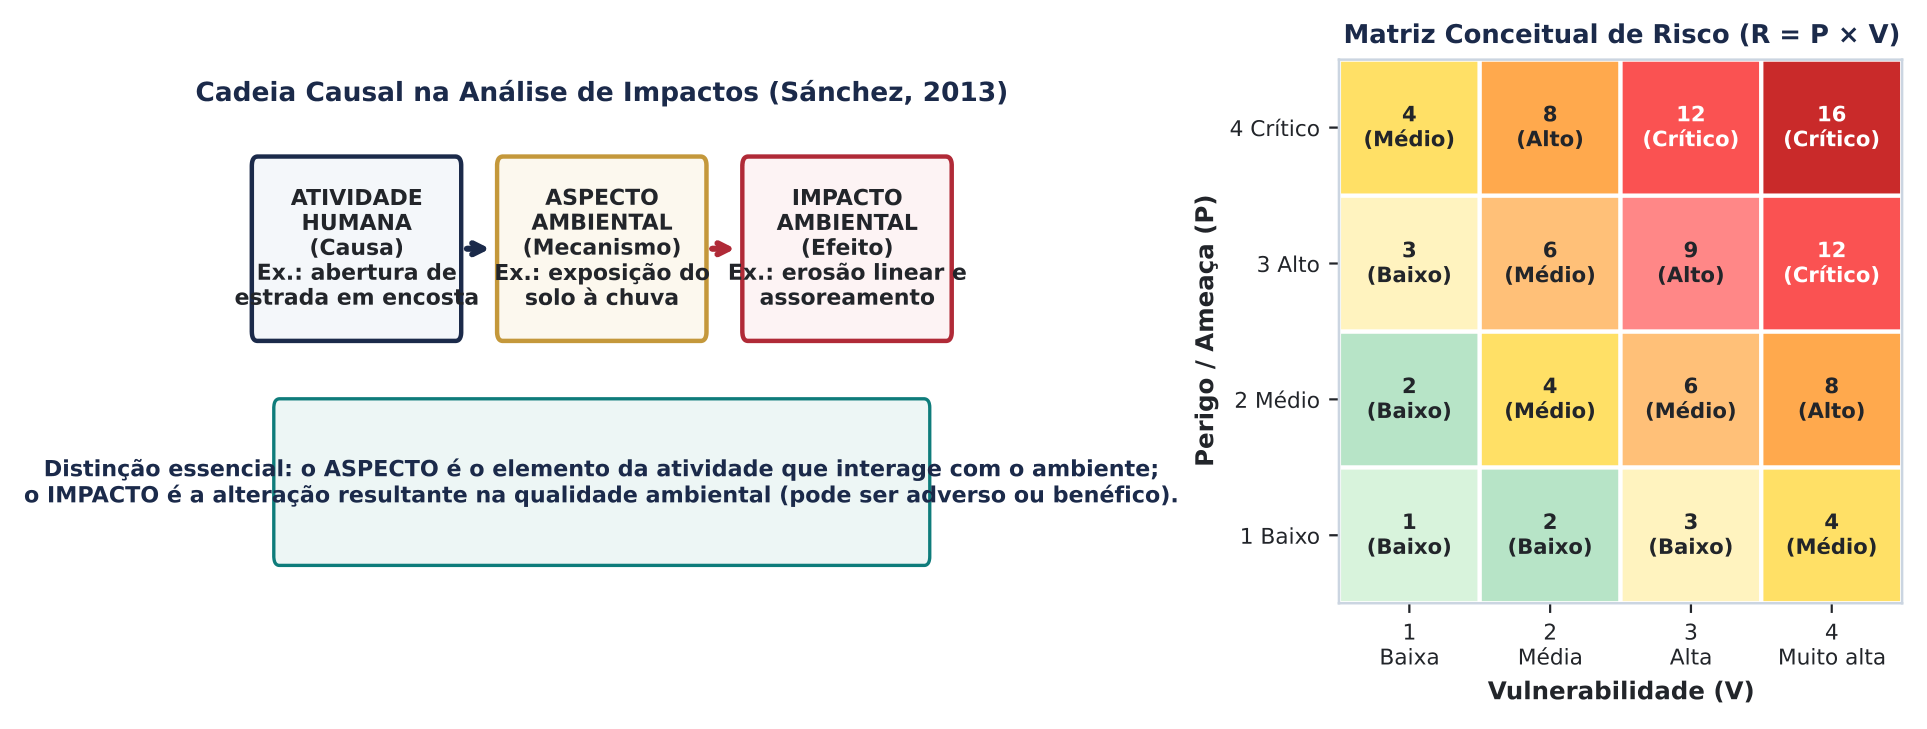
\includegraphics[keepaspectratio]{capitulos/../img/fig02_aspecto_impacto_risco.png}}

}

\caption{\label{fig-aspecto-risco}Conceitos operacionais centrais da
Análise Ambiental. \textbf{Painel esquerdo.} Cadeia causal Atividade
Humana \(\rightarrow\) Aspecto Ambiental \(\rightarrow\) Impacto
Ambiental segundo Sánchez (2013), destacando a diferença entre mecanismo
de interação (aspecto) e alteração na qualidade ambiental (impacto).
\textbf{Painel direito,} Matriz Conceitual de Risco Ambiental
(\(R = P \times V\)) em escala ordinal \(4 \times 4\), combinando níveis
de Perigo/Ameaça (\(P\)) e Vulnerabilidade (\(V\)) em quatro classes
operacionais (Baixo, Médio, Alto e Crítico).}

\end{figure}%

\subsection{\texorpdfstring{Equação e Matriz Conceitual do Risco
Ambiental
(\(R = P \times V\))}{Equação e Matriz Conceitual do Risco Ambiental (R = P \textbackslash times V)}}\label{equauxe7uxe3o-e-matriz-conceitual-do-risco-ambiental-r-p-times-v}

Na análise semiquantitativa de riscos socioambientais (alinhada ao
Painel direito da Figura~\ref{fig-aspecto-risco}), o índice de risco
ambiental \(R\) é obtido pelo produto do nível de \textbf{Perigo /
Ameaça (\(P\))} pelo nível de \textbf{Vulnerabilidade (\(V\))},

\[
R = P \times V
\]

em que,

\(P \in \{1, 2, 3, 4\}\), \(1 = \text{Baixo}\), \(2 = \text{Médio}\),
\(3 = \text{Alto}\), \(4 = \text{Crítico}\).
\(V \in \{0, 1, 2, 3, 4\}\), \(0 = \text{Nula}\) (ausência de exposição
humana ou infraestrutural, resultando em \(R = 0\)),
\(1 = \text{Baixa}\), \(2 = \text{Média}\), \(3 = \text{Alta}\),
\(4 = \text{Muito alta}\).

\textbf{Tabela da Matriz \(4 \times 4\) e Classes Operacionais de
Risco,}

{\def\LTcaptype{none} % do not increment counter
\begin{longtable}[]{@{}
  >{\raggedright\arraybackslash}p{(\linewidth - 8\tabcolsep) * \real{0.2000}}
  >{\raggedright\arraybackslash}p{(\linewidth - 8\tabcolsep) * \real{0.2000}}
  >{\raggedright\arraybackslash}p{(\linewidth - 8\tabcolsep) * \real{0.2000}}
  >{\raggedright\arraybackslash}p{(\linewidth - 8\tabcolsep) * \real{0.2000}}
  >{\raggedright\arraybackslash}p{(\linewidth - 8\tabcolsep) * \real{0.2000}}@{}}
\toprule\noalign{}
\begin{minipage}[b]{\linewidth}\raggedright
\textbf{Perigo (\(P\)) \(\backslash\) Vulnerabilidade (\(V\))}
\end{minipage} & \begin{minipage}[b]{\linewidth}\raggedright
\textbf{\(V = 1\) (Baixa)}
\end{minipage} & \begin{minipage}[b]{\linewidth}\raggedright
\textbf{\(V = 2\) (Média)}
\end{minipage} & \begin{minipage}[b]{\linewidth}\raggedright
\textbf{\(V = 3\) (Alta)}
\end{minipage} & \begin{minipage}[b]{\linewidth}\raggedright
\textbf{\(V = 4\) (Muito alta)}
\end{minipage} \\
\midrule\noalign{}
\endhead
\bottomrule\noalign{}
\endlastfoot
\textbf{\(P = 4\) (Crítico)} & \(4\) (Médio) & \(8\) (Alto) & \(12\)
(Crítico) & \(16\) (Crítico) \\
\textbf{\(P = 3\) (Alto)} & \(3\) (Baixo) & \(6\) (Médio) & \(9\) (Alto)
& \(12\) (Crítico) \\
\textbf{\(P = 2\) (Médio)} & \(2\) (Baixo) & \(4\) (Médio) & \(6\)
(Médio) & \(8\) (Alto) \\
\textbf{\(P = 1\) (Baixo)} & \(1\) (Baixo) & \(2\) (Baixo) & \(3\)
(Baixo) & \(4\) (Médio) \\
\end{longtable}
}

\textbf{Faixas de classificação (idênticas à
Figura~\ref{fig-aspecto-risco}),} \(1 \le R \le 3\), \textbf{Baixo}
\textbar{} \(4 \le R \le 6\), \textbf{Médio} \textbar{}
\(8 \le R \le 9\) (valores \(8\) e \(9\)), \textbf{Alto} \textbar{}
\(R \ge 12\) (valores \(12\) e \(16\)), \textbf{Crítico}.

\textbf{Cálculo passo a passo (efeito de redução de vulnerabilidade),}
Suponha uma comunidade em planície de inundação sujeita a perigo crítico
de cheia (\(P = 4\)) com vulnerabilidade alta (\(V_0 = 3\)). Após obras
de drenagem domiciliar, sistema de alerta precoce e elevação de soleiras
(sem alterar a magnitude da chuva/cheia no rio, mantendo \(P = 4\)), a
vulnerabilidade cai para média (\(V_1 = 2\)).

Risco inicial, \(R_0 = P \times V_0 = 4 \times 3 = 12\) (\textbf{Risco
Crítico}). Risco final, \(R_1 = P \times V_1 = 4 \times 2 = 8\)
(\textbf{Risco Alto}). Variação percentual do risco,

\[
\Delta R\% = \frac{R_1 - R_0}{R_0} \times 100\% = \frac{8 - 12}{12} \times 100\% = \frac{-4}{12} \times 100\% \approx -33{,}33\%.
\]

.

\textbf{Interpretação.} Mesmo quando o perigo natural não pode ser
eliminado (\(P = 4\)), reduzir a vulnerabilidade reduz o índice de risco
em \(33,33\%\), retirando o setor da faixa crítica.

\subsection{Resiliência, Recuperação, Restauração, Reabilitação e
Sustentabilidade}\label{resiliuxeancia-recuperauxe7uxe3o-restaurauxe7uxe3o-reabilitauxe7uxe3o-e-sustentabilidade}

Quando um ambiente já sofreu degradação, o analista ambiental precisa
avaliar sua capacidade de resposta espontânea e definir o objetivo
técnico viável de intervenção. Sánchez (2013) e a Lei do SNUC (Lei nº
9.985/2000, Art. 2º, XIII e XIV) diferenciam com rigor esses conceitos,

\textbf{Resiliência.} Capacidade de um ecossistema ou sistema
socioambiental absorver perturbações, reorganizar-se e manter suas
funções e processos essenciais, retornando a um estado funcional após um
distúrbio. Solos com boa matéria orgânica e bancos de sementes
preservados apresentam resiliência muito superior à de áreas decapadas
até a rocha matriz. \textbf{Recuperação ambiental.} Termo amplo
(conceito guarda-chuva técnico e legal) que designa a restituição de um
ecossistema ou de uma população silvestre degradada a uma \emph{condição
não degradada}, que pode ser diferente de sua condição original.

\textbf{Restauração ecológica.} Caso específico e mais exigente de
recuperação; consiste na restituição de um ecossistema degradado o mais
próximo possível de sua \emph{condição original} (estrutura, composição
de espécies nativas e funções ecológicas pré-distúrbio). É a meta
prioritária em Unidades de Conservação de proteção integral e APPs de
alto valor ecológico. \textbf{Reabilitação ambiental.} Retorno de uma
área degradada a um estado estável e funcional voltado a um \emph{novo
uso predefinido} (produtivo, urbano, paisagístico ou de lazer),
diferente da condição original, porém ambientalmente seguro e livre de
processos erosivos ou contaminação ativa. Exemplo, transformar uma
antiga pedreira urbana estabilizada em parque municipal com vegetação
adaptada.

\textbf{Remediação} (nota complementar de Sánchez, 2013), conjunto de
técnicas específicas para remover, conter ou neutralizar contaminantes
em áreas contaminadas (solo e água subterrânea), como postos de
combustíveis ou antigos lixões. \textbf{Sustentabilidade.} Princípio
orientador do planejamento que busca manter o uso dos recursos naturais
dentro da capacidade de suporte e regeneração dos ecossistemas,
integrando integridade ecológica, viabilidade econômica, justiça
socioespacial e responsabilidade intergeracional. Na literatura
ambiental, distingue-se a \emph{sustentabilidade fraca} (que admite
substituir capital natural por capital financeiro/tecnológico) da
\emph{sustentabilidade forte} (que reconhece funções ecológicas críticas
insubstituíveis, como água doce, solos férteis e biodiversidade).

{\def\LTcaptype{none} % do not increment counter
\begin{longtable}[]{@{}
  >{\raggedright\arraybackslash}p{(\linewidth - 4\tabcolsep) * \real{0.3333}}
  >{\raggedright\arraybackslash}p{(\linewidth - 4\tabcolsep) * \real{0.3333}}
  >{\raggedright\arraybackslash}p{(\linewidth - 4\tabcolsep) * \real{0.3333}}@{}}
\toprule\noalign{}
\begin{minipage}[b]{\linewidth}\raggedright
\textbf{Estratégia}
\end{minipage} & \begin{minipage}[b]{\linewidth}\raggedright
\textbf{Estado-Alvo}
\end{minipage} & \begin{minipage}[b]{\linewidth}\raggedright
\textbf{Quando Adotar na Prática}
\end{minipage} \\
\midrule\noalign{}
\endhead
\bottomrule\noalign{}
\endlastfoot
\textbf{Recuperação} & Condição não degradada (igual ou diferente da
original). & Termo técnico-legal geral adotado em PRAD e licenciamento
ambiental. \\
\textbf{Restauração} & O mais próximo possível da condição original
pré-distúrbio. & APPs, nascentes, unidades de conservação e áreas onde a
resiliência e os remanescentes permitem recomposição nativa. \\
\textbf{Reabilitação} & Novo uso estável, produtivo ou socialmente útil,
diferente do original. & Cavas de mineração urbana, áreas muito
alteradas em que o retorno ao estado original é inviável física ou
economicamente. \\
\textbf{Remediação} & Eliminação ou controle seguro de contaminantes
químicos. & Áreas contaminadas por hidrocarbonetos, chorume, metais
pesados ou agrotóxicos persistentes. \\
\end{longtable}
}

\subsection{Do conceito à variável
observável}\label{do-conceito-uxe0-variuxe1vel-observuxe1vel}

A abertura de uma estrada envolve corte, aterro e retirada de vegetação.
A exposição de solo e a concentração do escoamento constituem mecanismos
pelos quais a atividade modifica o ambiente. O aumento do aporte de
sedimentos a um curso de água representa uma alteração que pode ser
medida por campanhas comparáveis. A interrupção de uma captação
acrescenta uma consequência sobre um uso específico da água.

Uma matriz de risco organiza informações sobre possibilidade de
ocorrência, exposição e consequências segundo critérios previamente
definidos. Quando seus valores são classes ordinais, o produto entre
notas estabelece uma convenção de priorização. Um resultado igual a 12,
por exemplo, expressa a combinação adotada na matriz e não uma
probabilidade de 12\% nem uma previsão da quantidade de perdas.

O relatório precisa descrever como foram atribuídas as classes. A
frequência observada de eventos, o estado da drenagem, a distância dos
elementos expostos e a possibilidade de interrupção de serviços
sustentam a classificação. O registro de dados insuficientes é parte da
análise, pois orienta a próxima medição e impede que uma nota aparente
mais precisão do que a evidência disponível permite.

\section{Etapa 4 - Exemplos
resolvidos}\label{etapa-4---exemplos-resolvidos-3}

\subsection{Exemplo 4.1 - Cadeia Atividade-Aspecto-Impacto e
Classificação em Obra Urbana
(Básico)}\label{04-conceitos-operacionais-risco-exemplo-4.1.-cadeia-atividadeaspectoimpacto-e-classificauxe7uxe3o-em-obra-urbana-buxe1sico}

\textbf{Situação analisada.} A prefeitura de Feira de Santana realiza
uma obra de abertura de avenida marginal com drenagem pluvial ao longo
de um córrego urbano. Durante a terraplanagem em período chuvoso,
máquinas retiram a vegetação de barranco sem instalar barreiras de
contenção de sedimentos, gerando enxurrada barrenta que atinge o córrego
e assoreia um trecho de \(400\text{ m}\) a jusante. Estruture a cadeia
causal e classifique o impacto de assoreamento.

\textbf{Dados disponíveis.} Obra, abertura de avenida marginal. Ação em
campo, retirada de vegetação e exposição de solo sem contenção durante
chuvas. Consequência observada, carreamento de sedimentos e assoreamento
de \(400\text{ m}\) do córrego a jusante.

\textbf{Problema a resolver.} Separar atividade, aspecto ambiental e
impacto ambiental (direto e indireto), classificando o assoreamento
pelos critérios de Sánchez (2013).

\textbf{Fundamento da análise.} Cadeia causal da
Figura~\ref{fig-aspecto-risco} (Sánchez, 2013) e quadro de classificação
de impactos em sete atributos.

\textbf{Desenvolvimento.} \textbf{Passo 1, Cadeia causal,}

\textbf{Atividade humana (causa).} Terraplanagem para abertura da
avenida marginal. \textbf{Aspecto ambiental (mecanismo).} Supressão da
cobertura vegetal e exposição do solo solto à ação erosiva da chuva, com
carreamento de partículas para a drenagem. \textbf{Impacto ambiental
direto.} Erosão acelerada no talude da obra e aumento imediato da
turbidez da água. \textbf{Impacto ambiental indireto.} Assoreamento da
calha do córrego a jusante (\(400\text{ m}\)), reduzindo sua seção de
escoamento e ampliando o potencial de transbordamento.

\textbf{Passo 2, Classificação do impacto ``assoreamento a jusante'',}

Natureza, \textbf{adverso (negativo)};. Ordem causal, \textbf{indireto
(secundário)} (decorre da erosão do talude);. Prazo, \textbf{imediato a
médio prazo} (manifesta-se já nas primeiras chuvas intensas);. Duração,
\textbf{temporário a permanente} (persiste enquanto não houver
desassoreamento e estabilização da margem);. Reversibilidade,
\textbf{reversível} mediante manejo corretivo (contenção de taludes +
remoção controlada de sedimentos);. Abrangência, \textbf{local} (trecho
de \(400\text{ m}\) na microbacia urbana);. Interação,
\textbf{cumulativo} se somado a sedimentos oriundos de outros
loteamentos na mesma bacia.

\textbf{Interpretação do resultado.} Atividade, terraplanagem; Aspecto,
exposição de solo sem contenção; Impacto direto, erosão/turbidez;
Impacto indireto, assoreamento a jusante (adverso, indireto,
imediato/médio prazo, reversível mediante intervenção, local e
potencialmente cumulativo).

\textbf{Condições de validade.} A separação clara entre aspecto e
impacto permite atacar a causa (instalar barreiras de contenção,
biomantas e drenagem provisória sobre o solo exposto) antes que o
assoreamento se consolide.

\subsection{Exemplo 4.2 - Poluição vs.~Degradação Ambiental em Duas
Propriedades no Semiárido
(Básico)}\label{exemplo-4.2---poluiuxe7uxe3o-vs.-degradauxe7uxe3o-ambiental-em-duas-propriedades-no-semiuxe1rido-buxe1sico}

\textbf{Situação analisada.} Durante fiscalização técnica em uma
sub-bacia do Semiárido baiano, um analista avalia duas propriedades
rurais vizinhas, na Propriedade Alfa, o superpastejo contínuo removeu o
estrato herbáceo, compactou o solo e desencadeou sulcos e ravinas
profundas em encosta; na Propriedade Beta, um pequeno laticínio lança
soro de leite e água de lavagem sem tratamento diretamente em um riacho
intermitente, elevando a Demanda Bioquímica de Oxigênio (DBO) muito
acima dos limites do CONAMA e provocando mortandade de peixes nas poças
remanescentes. Classifique cada situação quanto a degradação ambiental e
poluição.

\textbf{Dados disponíveis.} Propriedade Alfa, superpastejo, solo
compactado e erosão em ravinas (sem lançamento de substâncias
químicas/efluentes). Propriedade Beta, lançamento de efluente orgânico
fora dos padrões legais, elevação de DBO e mortandade de peixes.

\textbf{Problema a resolver.} Determinar, com base na Lei nº 6.938/1981
e em Sánchez (2013), se cada caso configura degradação ambiental,
poluição ou ambos.

\textbf{Fundamento da análise.} Aplicação dos incisos II e III do Art.
3º da PNMA (gênero = degradação; espécie = poluição).

\textbf{Desenvolvimento.} \textbf{Passo 1, Análise da Propriedade Alfa.}
Ocorre alteração adversa severa das propriedades físicas e ecológicas do
solo (compactação, perda de cobertura, erosão em ravinas). Não há
lançamento de substância poluente em desacordo com padrões de emissão.
Portanto, há \textbf{degradação ambiental}, mas \textbf{não se
caracteriza poluição} em sentido estrito.\\
\textbf{Passo 2, Análise da Propriedade Beta.} Ocorre lançamento de
matéria orgânica em desacordo com os padrões ambientais vigentes,
afetando desfavoravelmente a biota (mortandade de peixes) e as condições
sanitárias da água. Como toda poluição constitui uma forma específica de
degradação, o caso configura simultaneamente \textbf{poluição hídrica} e
\textbf{degradação ambiental}.

\textbf{Interpretação do resultado.} Propriedade Alfa, degradação
ambiental sem poluição. Propriedade Beta, poluição hídrica e,
consequentemente, degradação ambiental.

\textbf{Condições de validade.} O enquadramento jurídico e técnico está
consistente com a relação de inclusão da PNMA (poluição \(\subset\)
degradação), orientando respostas distintas, manejo conservacionista do
solo/pastagem em Alfa e estação de tratamento de efluentes + autuação
por poluição em Beta.

\subsection{\texorpdfstring{Exemplo 4.3 - Cálculo Matricial e Redução
Percentual de Risco Ambiental (\(R = P \times V\))
(Intermediário)}{Exemplo 4.3 - Cálculo Matricial e Redução Percentual de Risco Ambiental (R = P \textbackslash times V) (Intermediário)}}\label{exemplo-4.3---cuxe1lculo-matricial-e-reduuxe7uxe3o-percentual-de-risco-ambiental-r-p-times-v-intermediuxe1rio}

\textbf{Situação analisada.} A Defesa Civil de um município do Recôncavo
Baiano mapeou três setores de uma vertente sujeita a escorregamentos
(Setores A, B e C) utilizando a matriz \(4 \times 4\) da
Figura~\ref{fig-aspecto-risco}. Posteriormente, no setor mais grave, a
prefeitura executou obras de drenagem superficial, estabilização de
talude com bioengenharia e realocação das casas mais precárias. Avalie o
risco inicial de cada setor e quantifique o efeito percentual da
intervenção.

\textbf{Dados disponíveis.} Cenário inicial, Setor A (\(P = 4\),
\(V = 4\)); Setor B (\(P = 3\), \(V = 3\)); Setor C (\(P = 4\),
\(V = 1\)). Cenário pós-intervenção no Setor A, o perigo foi reduzido de
\(4\) para \(3\) (drenagem e estabilização) e a vulnerabilidade de \(4\)
para \(2\) (realocação e reforço estrutural).

\textbf{Problema a resolver.} Calcular \(R = P \times V\) e classificar
os setores A, B e C antes da obra; calcular o novo risco de A e a
variação percentual \(\Delta R\%\).

\textbf{Fundamento da análise.} Aplicação da equação \(R = P \times V\),
das faixas da Figura~\ref{fig-aspecto-risco} (1 a 3 Baixo; 4 a 6 Médio;
8 a 9 Alto; 12 a 16 Crítico) e de
\(\Delta R\% = \frac{R_1 - R_0}{R_0}\times 100\%\).

\textbf{Desenvolvimento.} \textbf{Passo 1, Cálculo inicial dos três
setores,}

Setor A, \(R_A = 4 \times 4 = 16\) (\textbf{Risco Crítico}). Setor B,
\(R_B = 3 \times 3 = 9\) (\textbf{Risco Alto}). Setor C,
\(R_C = 4 \times 1 = 4\) (\textbf{Risco Médio}).

\textbf{Passo 2, Comparação crítica entre B e C.} Observe que o Setor C
possui perigo maior (\(P = 4\)) do que o Setor B (\(P = 3\)), mas seu
risco (\(R_C = 4\)) é menos da metade do risco de B (\(R_B = 9\)) porque
a vulnerabilidade em C é baixa (\(V = 1\)).\\
\textbf{Passo 3, Cenário pós-intervenção no Setor A (\(P_1 = 3\),
\(V_1 = 2\)),}

\[
R_{A,\text{final}} = 3 \times 2 = 6 \quad (\textbf{Risco Médio}).
\]

\textbf{Passo 4, Variação percentual do risco no Setor A,}

\[
\Delta R\% = \frac{6 - 16}{16} \times 100\% = \frac{-10}{16} \times 100\% = -0{,}625 \times 100\% = -62{,}50\%.
\]

\textbf{Interpretação do resultado.} Inicial, Setor A = \(16\)
(Crítico), Setor B = \(9\) (Alto), Setor C = \(4\) (Médio). Após
intervenção no Setor A, \(R = 6\) (Médio), representando redução de
\(62,50\%\) no índice de risco.

\textbf{Condições de validade.} O resultado faz pleno sentido matemático
(\(6/16 = 37,5\%\) do risco original, logo queda de \(62,5\%\)) e
operacional, demonstrando que atuar simultaneamente sobre o perigo
(engenharia/bioengenharia) e sobre a vulnerabilidade
(ordenamento/habitação) produz redução expressiva de risco.

\subsection{Exemplo 4.4 - Fragilidade Ambiental vs.~Perigo vs.~Risco em
Vertentes da Caatinga
(Intermediário)}\label{exemplo-4.4---fragilidade-ambiental-vs.-perigo-vs.-risco-em-vertentes-da-caatinga-intermediuxe1rio}

\textbf{Situação analisada.} Considere duas vertentes
geomorfologicamente idênticas no Semiárido baiano, ambas possuem
\(38\%\) de declividade, Neossolo Litólico raso e chuvas concentradas de
alta erosividade. A Vertente 1 localiza-se no interior de um Parque
Estadual preservado, sem estradas nem moradores. A Vertente 2 teve sua
vegetação suprimida e recebeu um loteamento residencial irregular na
base da encosta. Compare fragilidade ambiental, perigo, vulnerabilidade
e risco nas duas vertentes.

\textbf{Dados disponíveis.} Vertente 1, declividade \(38\%\), solo raso,
vegetação de Caatinga preservada, sem população ou bens expostos.
Vertente 2, mesma declividade e solo, vegetação suprimida, loteamento
irregular na base.

\textbf{Problema a resolver.} Diferenciar conceitualmente a condição de
cada vertente quanto a fragilidade potencial, perigo, vulnerabilidade e
risco socioambiental.

\textbf{Fundamento da análise.} Distinção rigorosa entre fragilidade
intrínseca do meio físico, ameaça física, exposição humana e risco
(Seção 4.4).

\textbf{Desenvolvimento.} \textbf{Passo 1, Fragilidade potencial (meio
físico).} Ambas as vertentes apresentam \textbf{alta fragilidade
natural/potencial}, pois compartilham declividade elevada (\(38\%\)),
solo raso e chuvas erosivas. Na Vertente 1, porém, a cobertura vegetal
conservada protege o solo (menor fragilidade emergente); na Vertente 2,
a supressão vegetal eleva a instabilidade.\\
\textbf{Passo 2, Perigo / Ameaça (\(P\)).} Em ambas existe potencial
físico de escoamento rápido e queda de material, porém acentuado na
Vertente 2 pela retirada da vegetação e pelos cortes de talude do
loteamento.\\
\textbf{Passo 3, Vulnerabilidade (\(V\)).} Na Vertente 1, não há
pessoas, habitações ou infraestruturas expostas (\(V = 0\) do ponto de
vista socioambiental humano). Na Vertente 2, há moradias precárias
diretamente na zona de impacto (\(V\) alta ou muito alta).\\
\textbf{Passo 4, Risco Socioambiental (\(R\)).} Na Vertente 1, apesar da
alta fragilidade física, o risco de desastre humano é \textbf{nulo}
(\(R = P \times 0 = 0\)). Na Vertente 2, a convergência entre alto
perigo e alta vulnerabilidade gera \textbf{risco alto ou crítico}.

\textbf{Interpretação do resultado.} Ambas possuem alta fragilidade
física potencial, mas apenas a Vertente 2 apresenta risco socioambiental
humano elevado, em virtude da exposição de moradores vulneráveis e da
desestabilização antrópica da cobertura vegetal.

\textbf{Condições de validade.} Esse contraste comprova por que mapas de
fragilidade física não devem ser rotulados automaticamente como ``mapas
de risco'' sem cruzar o dado de exposição e vulnerabilidade social.

\subsection{Exemplo 4.5 - Escolha entre Restauração e Reabilitação em
Passivo Minerário
(Avançado)}\label{exemplo-4.5---escolha-entre-restaurauxe7uxe3o-e-reabilitauxe7uxe3o-em-passivo-mineruxe1rio-avanuxe7ado}

\textbf{Situação analisada.} Na planície fluvial do Rio Jacuípe (BA),
uma área de \(8\text{ ha}\) usada por 15 anos para extração irregular de
areia deixou cavas com \(4\text{ m}\) de profundidade que atingiram o
lençol freático, margens instáveis em desmoronamento e perda completa do
horizonte A do solo. A área está hoje cercada por expansão urbana e por
pequenas lavouras que aplicam fertilizantes solúveis. O Ministério
Público exigiu um PRAD. Discuta a resiliência local, o potencial impacto
cumulativo/sinérgico com as lavouras vizinhas e justifique tecnicamente
a escolha entre restauração ecológica integral e reabilitação ambiental.

\textbf{Dados disponíveis.} Passivo, \(8\text{ ha}\), cavas de
\(4\text{ m}\) atingindo o lençol freático, margens instáveis, ausência
de solo superficial, entorno urbano e agrícola com fertilizantes.
Exigência legal, PRAD.

\textbf{Problema a resolver.} Avaliar (a) a resiliência do sistema, (b)
a possibilidade de impacto sinérgico com o entorno e (c) a estratégia
mais adequada (restauração vs.~reabilitação).

\textbf{Fundamento da análise.} Critérios de resiliência, impactos
cumulativos/sinérgicos e distinção recuperação/restauração/reabilitação
segundo Sánchez (2013) e Lei do SNUC.

\textbf{Desenvolvimento.} \textbf{Passo 1, Avaliação da resiliência.} A
resiliência natural está severamente comprometida (\textbf{muito
baixa}). A remoção de \(4\text{ m}\) de sedimento eliminou o horizonte
superficial, a matéria orgânica e o banco de sementes, alterando
irreversivelmente a topografia e expondo a água subterrânea. A
regeneração espontânea não restituirá a floresta ciliar original.\\
\textbf{Passo 2, Impacto sinérgico com as lavouras.} O escoamento
superficial carregando nutrientes das lavouras vizinhas (aspecto
agrícola) encontra o lençol freático exposto nas cavas estagnadas
(aspecto minerário). A combinação desses dois processos distintos gera
eutrofização acelerada e risco de contaminação do aquífero, efeito mais
intenso do que cada atividade isolada (\textbf{impacto sinérgico}).\\
\textbf{Passo 3, Escolha entre restauração e reabilitação.} A
\textbf{restauração ecológica integral} (retorno exato à planície
original pré-mineração) exigiria milhões de metros cúbicos de material
de aterro externo, criando novas áreas degradadas de empréstimo e
tornando-se ambiental e economicamente inviável. A estratégia
tecnicamente recomendada é a \textbf{reabilitação ambiental} (inserida
no guarda-chuva legal da recuperação), retaludamento e estabilização das
margens das cavas com bioengenharia, implantação de faixa tampão de
vegetação nativa ciliar (filtrando nutrientes das lavouras) e conversão
das lagoas estabilizadas em parque ecológico/área de amortecimento
hídrico seguro.

\textbf{Interpretação do resultado.} Resiliência muito baixa; risco de
impacto sinérgico (eutrofização e contaminação do aquífero pela
interação cava aberta + fertilizantes); estratégia indicada,
\textbf{reabilitação ambiental} associada à faixa tampão vegetada nativa
nas bordas, descartando a restauração topográfica integral por
inviabilidade física e ecológica.

\textbf{Condições de validade.} A decisão respeita a legislação (o PRAD
exige recuperação, que admite reabilitação quando o retorno ao estado
original é impraticável) e neutraliza tanto a instabilidade geotécnica
das margens quanto a vulnerabilidade do lençol freático.

\section{Etapa 5 - Erros de
interpretação}\label{etapa-5---erros-de-interpretauxe7uxe3o-3}

\subsection{Erro 1, Confundir Aspecto Ambiental com Impacto
Ambiental}\label{erro-1-confundir-aspecto-ambiental-com-impacto-ambiental}

\textbf{Equívoco frequente.} Listar em uma matriz de AIA o
``desmatamento'' ou o ``lançamento de esgoto'' na coluna de
\emph{impactos ambientais}.\\
\textbf{Por que está incorreto.} Desmatamento (supressão vegetal) e
lançamento de esgoto são \textbf{aspectos ambientais} (mecanismos pelos
quais a atividade interage com o meio). Os \textbf{impactos} são as
alterações resultantes na qualidade ambiental, perda de habitat, erosão
laminar, redução do oxigênio dissolvido ou mortandade de peixes.\\
\textbf{Como evitar.} Teste sempre a frase com o conector ``provoca'',
\emph{Atividade} gera \emph{Aspecto}, que \textbf{provoca}
\emph{Impacto}.

\subsection{Erro 2, Tratar Todo Impacto como Negativo e Igualar Poluição
a
Degradação}\label{erro-2-tratar-todo-impacto-como-negativo-e-igualar-poluiuxe7uxe3o-a-degradauxe7uxe3o}

\textbf{Equívoco frequente.} Afirmar que ``não há impacto ambiental em
projetos de recuperação'' ou dizer que ``a erosão do solo por pastoreio
é um caso de poluição''.\\
\textbf{Por que está incorreto.} Projetos de recuperação geram
\textbf{impactos ambientais benéficos} (positivos); além disso, erosão
sem lançamento de substâncias em desacordo com padrões legais é
\textbf{degradação ambiental}, mas não necessariamente poluição.\\
\textbf{Como evitar.} Qualifique sempre o impacto (adverso ou benéfico)
e verifique se houve lançamento de matéria/energia ou alteração
sanitária prevista no Art. 3º, III da PNMA antes de usar o termo
poluição.

\subsection{Erro 3, Confundir Fragilidade Ambiental ou Perigo com
Risco}\label{erro-3-confundir-fragilidade-ambiental-ou-perigo-com-risco}

\textbf{Equívoco frequente.} Chamar um mapa de declividade ou de
erodibilidade de ``mapa de risco ambiental'' sem considerar a presença e
a vulnerabilidade da população ou da infraestrutura.\\
\textbf{Por que está incorreto.} Declividade e erodibilidade expressam
\textbf{fragilidade} ou \textbf{perigo físico (\(P\))}. Sem
vulnerabilidade (\(V > 0\)), não há risco socioambiental
(\(R = P \times V\)).\\
\textbf{Como evitar.} Verifique se os dois fatores (\(P\) e \(V\)) estão
explicitamente presentes no diagnóstico antes de empregar a palavra
risco.

\subsection{Erro 4, Prometer ``Restauração Integral'' Onde Apenas a
Reabilitação é
Viável}\label{erro-4-prometer-restaurauxe7uxe3o-integral-onde-apenas-a-reabilitauxe7uxe3o-uxe9-viuxe1vel}

\textbf{Equívoco frequente.} Redigir em um PRAD que uma cava profunda de
mineração ou uma área urbana aterrada será ``integralmente restaurada à
sua condição original''.\\
\textbf{Por que está incorreto.} A restauração exige aproximação máxima
da estrutura, composição e funções originais pré-distúrbio, o que
frequentemente é impossível após alterações geomorfológicas
irreversíveis. Promessas inexequíveis levam à rejeição do PRAD ou ao
descumprimento de condicionantes.\\
\textbf{Como evitar.} Avalie a resiliência e o grau de alteração do
relevo/solo; use \textbf{restauração} apenas quando o retorno ao
ecossistema de referência for factível, e \textbf{reabilitação} quando o
objetivo for um novo uso estável e seguro.

\section{Etapa 6 - Exercícios de
fixação}\label{etapa-6---exercuxedcios-de-fixauxe7uxe3o-3}

\subsubsection{Nível Básico (Exercícios 1 a
5)}\label{nuxedvel-buxe1sico-exercuxedcios-1-a-5-1}

\begin{enumerate}
\def\labelenumi{\arabic{enumi}.}
\item
  Apresente a definição legal de \textbf{meio ambiente} segundo a Lei nº
  6.938/1981 (PNMA) e explique por que Sánchez (2013) recomenda incluir
  explicitamente o meio construído e as relações socioeconômicas na
  Análise Ambiental.
\item
  Para a atividade humana ``operação de uma indústria cerâmica de
  pequeno porte'', cite um exemplo de \textbf{aspecto ambiental} e um
  exemplo do correspondente \textbf{impacto ambiental}.
\item
  Explique a diferença entre \textbf{impacto cumulativo} e
  \textbf{impacto sinérgico}, apresentando um exemplo prático para cada
  um em uma bacia hidrográfica.
\item
  Justifique a afirmação, \emph{``Toda poluição provoca degradação
  ambiental, mas nem toda degradação ambiental é poluição.''}
\item
  Defina \textbf{resiliência ambiental} e explique por que um solo
  decapado até a rocha apresenta resiliência muito menor do que uma
  pastagem abandonada cercada por fragmentos de mata nativa.
\end{enumerate}

\subsubsection{Nível Intermediário (Exercícios 6 a
10)}\label{nuxedvel-intermediuxe1rio-exercuxedcios-6-a-10-1}

\begin{enumerate}
\def\labelenumi{\arabic{enumi}.}
\setcounter{enumi}{5}
\item
  Uma encosta ocupada (Encosta X) foi avaliada inicialmente com Perigo
  Alto (\(P_0 = 3\)) e Vulnerabilidade Muito Alta (\(V_0 = 4\)). Após
  obras de retaludamento, drenagem pluvial e melhoria estrutural das
  moradias, os indicadores caíram para Perigo Médio (\(P_1 = 2\)) e
  Vulnerabilidade Média (\(V_1 = 2\)). Calcule passo a passo, (a) o
  risco inicial \(R_0\) e sua classe; (b) o risco final \(R_1\) e sua
  classe; (c) a variação percentual \(\Delta R\%\).
\item
  Compare duas margens de rio urbano usando a matriz \(4 \times 4\) da
  Figura~\ref{fig-aspecto-risco}, a \textbf{Margem Y} tem \(P = 4\) e
  \(V = 3\); a \textbf{Margem Z} tem \(P = 3\) e \(V = 2\). Determine o
  índice e a classe de risco de cada margem e indique qual delas deve
  receber prioridade emergencial de intervenção, justificando.
\item
  A implantação de uma Estação de Tratamento de Esgoto (ETE) municipal
  gera ruído temporário durante os 8 meses de obras, mas, após entrar em
  operação, reduz em \(85\%\) a carga orgânica lançada no rio local
  durante décadas. Classifique esses dois impactos segundo os critérios
  de \textbf{natureza}, \textbf{duração} e \textbf{reversibilidade}.
\item
  Diferencie \textbf{fragilidade ambiental}, \textbf{perigo} e
  \textbf{risco} no contexto de um paredão rochoso instável localizado,
  (a) em área desabitada de parque estadual; (b) imediatamente acima de
  uma rodovia federal movimentada.
\item
  Uma pedreira de granito desativada na periferia de uma cidade média do
  Nordeste possui paredões verticais de \(18\text{ m}\) e piso
  totalmente rochoso. Entre \textbf{restauração ecológica} e
  \textbf{reabilitação ambiental}, qual alternativa é tecnicamente mais
  adequada? Justifique sua escolha.
\end{enumerate}

\subsubsection{Nível Aplicado, Questões Objetivas (Exercícios 11 a
15)}\label{nuxedvel-aplicado-questuxf5es-objetivas-exercuxedcios-11-a-15-1}

\begin{enumerate}
\def\labelenumi{\arabic{enumi}.}
\setcounter{enumi}{10}
\item
  Na cadeia causal apresentada por Sánchez (2013) e na
  Figura~\ref{fig-aspecto-risco}, ao analisar a atividade ``aplicação de
  fertilizantes em área agrícola declivosa'', constitui um
  \textbf{aspecto ambiental} e o seu respectivo \textbf{impacto
  ambiental}, nessa ordem,

  \begin{enumerate}
  \def\labelenumii{(\Alph{enumii})}
  \item
    Eutrofização do açude; carreamento de nitrogênio e fósforo pela
    enxurrada.
  \item
    Carreamento de nutrientes pela enxurrada para o corpo d'água;
    eutrofização do açude e proliferação de algas.
  \item
    Aplicação de fertilizantes; compra de insumos agrícolas.
  \item
    Proliferação de algas; abertura de estrada rural.
  \item
    Redução do oxigênio dissolvido; emissão de licença ambiental.
  \end{enumerate}
\item
  Em uma bacia hidrográfica do Semiárido, cinco pequenas indústrias
  lançam efluentes tratados dentro do padrão individual, mas a soma das
  cargas ao longo do rio reduz gradualmente a qualidade da água na foz.
  Esse fenômeno caracteriza um impacto tipicamente,

  \begin{enumerate}
  \def\labelenumii{(\Alph{enumii})}
  \item
    Benéfico e pontual.
  \item
    Irreversível e imediato apenas na fonte.
  \item
    Cumulativo.
  \item
    Natural e não antrópico.
  \item
    Estético sem alteração físico-química.
  \end{enumerate}
\item
  Segundo a Matriz Conceitual de Risco (\(R = P \times V\), escala \(1\)
  a \(4\) da Figura~\ref{fig-aspecto-risco}), uma área classificada com
  Perigo Crítico (\(P = 4\)) e Vulnerabilidade Baixa (\(V = 1\))
  apresenta,

  \begin{enumerate}
  \def\labelenumii{(\Alph{enumii})}
  \item
    \(R = 16\) (Risco Crítico).
  \item
    \(R = 12\) (Risco Crítico).
  \item
    \(R = 8\) (Risco Alto).
  \item
    \(R = 4\) (Risco Médio).
  \item
    \(R = 2\) (Risco Baixo).
  \end{enumerate}
\item
  De acordo com a Lei do SNUC (Lei nº 9.985/2000) e com Sánchez (2013),
  a restituição de um ecossistema degradado a uma condição \textbf{o
  mais próximo possível da sua condição original} denomina-se,

  \begin{enumerate}
  \def\labelenumii{(\Alph{enumii})}
  \item
    Remediação.
  \item
    Reabilitação.
  \item
    Restauração.
  \item
    Compensação financeira.
  \item
    Mitigação preventiva.
  \end{enumerate}
\item
  Sobre o conceito de \textbf{sustentabilidade forte}, em contraste com
  a sustentabilidade fraca, é correto afirmar que,

  \begin{enumerate}
  \def\labelenumii{(\Alph{enumii})}
  \item
    Admite substituir integralmente ecossistemas críticos por capital
    financeiro ou infraestrutura artificial.
  \item
    Reconhece que determinadas funções ecológicas e estoques naturais
    críticos (como água doce, solos férteis e biodiversidade) são
    insubstituíveis e impõem limites biofísicos ao crescimento
    econômico.
  \item
    Aplica-se exclusivamente a unidades de conservação sem presença
    humana no entorno.
  \item
    Desconsidera a justiça social e a dimensão intergeracional na gestão
    ambiental.
  \item
    Equivale à compensação pecuniária automática de qualquer dano
    irreversível.
  \end{enumerate}
\end{enumerate}

\section{Etapa 7 - Questões de
aplicação}\label{etapa-7---questuxf5es-de-aplicauxe7uxe3o-3}

\subsection{Estratégia para o Estudo Orientado 3 (EO3) e para a
Avaliação
Teórica}\label{estratuxe9gia-para-o-estudo-orientado-3-eo3-e-para-a-avaliauxe7uxe3o-teuxf3rica}

No \textbf{EO3} (Semana 4, baseado em Sánchez, 2013, cap. 1, e
Tauk-Tornisielo, 1996) e em concursos para Analista Ambiental (IBAMA,
ICMBio, INEMA), há três pegadinhas recorrentes que você agora sabe
desarmar,

\begin{enumerate}
\def\labelenumi{\arabic{enumi}.}
\item
  \textbf{Aspecto \(\neq\) Impacto.} Leia o enunciado identificando se a
  frase descreve a interação (aspecto) ou a mudança no estado do meio
  (impacto).
\item
  \textbf{Degradação \(\supset\) Poluição.} Verifique se há lançamento
  de poluente/alteração sanitária ou apenas degradação física/ecológica
  (como erosão e desmatamento).
\item
  \textbf{Restauração \(\neq\) Reabilitação \(\neq\) Recuperação.}
  Lembre que \emph{recuperação} é o termo geral (condição não degradada,
  igual ou diferente da original), enquanto \emph{restauração} busca o
  estado original e \emph{reabilitação} destina a área a um novo uso
  funcional estável.
\end{enumerate}

\begin{enumerate}
\def\labelenumi{\arabic{enumi}.}
\setcounter{enumi}{15}
\item
  \textbf{(Questão autoral, estilo Concurso Analista Ambiental / IBAMA)}
  Com base na Política Nacional do Meio Ambiente (Lei nº 6.938/1981), na
  Resolução CONAMA nº 01/1986 e na obra de Sánchez (2013), julgue as
  proposições abaixo,

  \begin{enumerate}
  \def\labelenumii{\Roman{enumii}.}
  \item
    Um impacto ambiental é necessariamente negativo, razão pela qual
    programas de recuperação florestal não produzem impactos ambientais.
  \item
    A remoção da vegetação ciliar com consequente assoreamento de curso
    d'água constitui degradação ambiental mesmo que não haja lançamento
    de efluentes químicos tóxicos.
  \item
    A interação entre dois impactos distintos cujo efeito conjunto é
    maior do que a soma de seus efeitos isolados define o caráter
    sinérgico do impacto.
  \item
    A exposição do solo decorrente da abertura de uma estrada é o
    aspecto ambiental, enquanto a perda de solo por erosão laminar e o
    aumento da turbidez no córrego são os impactos ambientais.
  \end{enumerate}

  Estão corretas apenas as proposições,

  \begin{enumerate}
  \def\labelenumii{(\Alph{enumii})}
  \item
    I e II.
  \item
    I e III.
  \item
    II e IV.
  \item
    II, III e IV.
  \item
    I, II, III e IV.
  \end{enumerate}
\item
  \textbf{(Questão autoral, estilo ENADE / Geografia)} Duas comunidades
  localizam-se na mesma bacia hidrográfica semiárida, submetidas a
  eventos de enxurrada súbita de igual intensidade (mesmo perigo físico
  \(P = 3\)). A Comunidade 1 possui sistema de drenagem pluvial,
  construções em alvenaria fora da cota máxima de cheia e plano de
  alerta comunitário (\(V = 1\)). A Comunidade 2 ocupa precariamente a
  planície de inundação, sem drenagem nem alerta (\(V = 4\)). À luz dos
  conceitos operacionais de perigo, vulnerabilidade e risco
  (\(R = P \times V\)), assinale a alternativa correta,

  \begin{enumerate}
  \def\labelenumii{(\Alph{enumii})}
  \item
    Ambas as comunidades possuem o mesmo risco ambiental, pois estão
    expostas à mesma intensidade pluviométrica (\(P = 3\)).
  \item
    A Comunidade 1 apresenta risco baixo (\(R = 3\)) e a Comunidade 2
    apresenta risco crítico (\(R = 12\)), demonstrando o peso
    determinante da vulnerabilidade socioespacial na produção de
    desastres.
  \item
    A Comunidade 2 apresenta risco médio (\(R = 7\)), resultado da soma
    entre perigo (\(3\)) e vulnerabilidade (\(4\)).
  \item
    A vulnerabilidade é uma propriedade estritamente geológica do
    terreno, independente da renda, da infraestrutura e da localização
    das moradias.
  \item
    Para reduzir o risco da Comunidade 2, a única medida tecnicamente
    possível consiste em modificar o regime climático regional para
    eliminar a chuva intensa.
  \end{enumerate}
\item
  \textbf{(Questão autoral, estilo Concurso Perito Ambiental / INEMA)}
  Um empreendimento de extração de argila abandonou, há dez anos, uma
  área de \(12\text{ ha}\) sem solo superficial, com cavas alagadas e
  taludes instáveis em periferia urbana. O laudo pericial constatou
  resiliência natural muito baixa e propôs estabilizar os taludes,
  revegetar as margens com espécies nativas e integrar o espelho d'água
  a um parque urbano de retenção de cheias, deixando claro que não será
  possível reconstituir o relevo e a floresta originais.
  Conceitualmente, a intervenção proposta corresponde à,

  \begin{enumerate}
  \def\labelenumii{(\Alph{enumii})}
  \item
    Restauração ecológica integral, pois utiliza espécies nativas nas
    margens.
  \item
    Remediação química, visto que a área estava abandonada há dez anos.
  \item
    Reabilitação ambiental, modalidade de recuperação que destina a área
    degradada a um novo uso estável e funcional distinto da condição
    original.
  \item
    Degradação controlada, uma vez que não se recompõe a topografia
    pré-mineração.
  \item
    Sustentabilidade fraca ilegal, pois o SNUC proíbe qualquer
    intervenção que não reconstitua integralmente o estado original.
  \end{enumerate}
\end{enumerate}

\section{Etapa 8 - Gabarito
comentado}\label{etapa-8---gabarito-comentado-3}

\subsection{Resolução, Nível Básico (Exercícios 1 a
5)}\label{resoluuxe7uxe3o-nuxedvel-buxe1sico-exercuxedcios-1-a-5-1}

\begin{enumerate}
\def\labelenumi{\arabic{enumi}.}
\item
  \textbf{Meio ambiente (PNMA e Sánchez, 2013).} Pela Lei nº 6.938/1981
  (Art. 3º, I), meio ambiente é o conjunto de condições, leis,
  influências e interações de ordem física, química e biológica que
  permite, abriga e rege a vida em todas as suas formas. Sánchez (2013)
  destaca a inclusão do meio construído e das relações socioeconômicas
  porque as atividades humanas transformam continuamente os sistemas
  naturais e os impactos ambientais atingem diretamente a saúde, a
  economia, o patrimônio e o bem-estar social (como reconhece a
  Resolução CONAMA nº 01/1986).
\item
  \textbf{Indústria cerâmica (aspecto e impacto),} \emph{Aspecto
  ambiental,} emissão de fumaça e material particulado pela queima de
  lenha nos fornos (ou extração de argila em várzea). \emph{Impacto
  ambiental correspondente,} degradação da qualidade do ar e agravo a
  doenças respiratórias no entorno (ou desestabilização de margens e
  perda de vegetação ciliar).
\item
  \textbf{Cumulativo vs.~Sinérgico,} \emph{Cumulativo} resulta da soma
  de impactos semelhantes ao longo do tempo ou de diversas fontes (por
  exemplo, múltiplos barramentos rurais em uma bacia reduzindo
  progressivamente a vazão no exutório). \emph{Sinérgico} resulta da
  interação entre dois ou mais impactos distintos cujo efeito combinado
  supera a soma isolada das partes (por exemplo, remoção de mata ciliar
  somada ao lançamento de esgoto doméstico, acelerando conjuntamente o
  assoreamento e a eutrofização severa do rio).
\item
  \textbf{Poluição \(\subset\) Degradação.} Pela PNMA (Art. 3º, II e
  III), degradação é o gênero (qualquer alteração adversa do meio),
  enquanto poluição é uma espécie específica de degradação (ligada a
  prejuízos à saúde/biota/bem-estar ou lançamento de matéria/energia
  fora dos padrões). Logo, toda poluição degrada o ambiente, mas
  processos como desmatamento, compactação e erosão degradam o ambiente
  sem necessariamente envolver poluição química.
\item
  \textbf{Resiliência.} Capacidade do sistema absorver perturbações e
  recuperar estrutura e funções essenciais. O solo decapado até a rocha
  perdeu horizonte orgânico, estrutura porosa, retenção hídrica e banco
  de sementes (resiliência muito baixa); já a pastagem cercada por
  fragmentos nativos preserva solo e fonte próxima de propágulos
  (sementes e dispersores), conferindo resiliência muito mais alta.
\end{enumerate}

\subsection{Resolução, Nível Intermediário (Exercícios 6 a
10)}\label{resoluuxe7uxe3o-nuxedvel-intermediuxe1rio-exercuxedcios-6-a-10-1}

\begin{enumerate}
\def\labelenumi{\arabic{enumi}.}
\setcounter{enumi}{5}
\item
  \textbf{Cálculo passo a passo do risco na Encosta X,}

  \begin{itemize}
  \item
    (a) Risco inicial,
    \(R_0 = P_0 \times V_0 = 3 \times 4 = \mathbf{12}\) (\textbf{Risco
    Crítico}, pois \(R \ge 12\)).
  \item
    (b) Risco final, \(R_1 = P_1 \times V_1 = 2 \times 2 = \mathbf{4}\)
    (\textbf{Risco Médio}, faixa \(4 \le R \le 6\)).
  \item
    (c) Variação percentual,
  \end{itemize}

  \[
   \Delta R\% = \frac{R_1 - R_0}{R_0} \times 100\% = \frac{4 - 12}{12} \times 100\% = \frac{-8}{12} \times 100\% = -\frac{2}{3} \times 100\% \approx \mathbf{-66{,}67\%}.
   \]

  A intervenção reduziu o índice de risco em \(66,67\%\), deslocando a
  encosta da classe Crítica para a classe Média.
\item
  \textbf{Comparação Margem Y vs.~Margem Z,}

  \begin{itemize}
  \item
    Margem Y, \(R_Y = 4 \times 3 = \mathbf{12}\) (\textbf{Risco
    Crítico}).
  \item
    Margem Z, \(R_Z = 3 \times 2 = \mathbf{6}\) (\textbf{Risco Médio}).
  \item
    \textbf{Prioridade.} A \textbf{Margem Y} deve receber intervenção
    emergencial prioritária, pois possui o dobro do índice de risco de Z
    e encontra-se na faixa crítica (\(R = 12\)).
  \end{itemize}
\item
  \textbf{Classificação dos impactos da ETE,}

  \begin{itemize}
  \item
    \emph{Ruído durante 8 meses de obras,} natureza \textbf{adversa},
    duração \textbf{temporária}, \textbf{reversível} (cessa
    imediatamente ao término da obra).
  \item
    \emph{Redução de \(85\%\) da carga orgânica no rio,} natureza
    \textbf{benéfica}, duração \textbf{permanente} (enquanto a ETE
    operar adequadamente), \textbf{reversível} caso a estação deixe de
    receber manutenção.
  \end{itemize}
\item
  \textbf{Paredão rochoso instável,}

  \begin{itemize}
  \item
    (a) \emph{Parque desabitado,} alta \textbf{fragilidade} física e
    existência de \textbf{perigo} de queda de blocos (\(P > 0\)), mas
    sem elementos humanos expostos (\(V = 0\)), logo \textbf{risco
    humano nulo}.
  \item
    (b) \emph{Acima de rodovia movimentada,} mesma fragilidade e perigo
    físico, agora combinados com alta exposição de veículos e
    passageiros (\(V > 0\)), configurando \textbf{risco socioambiental
    elevado} que exige obras de contenção e monitoramento.
  \end{itemize}
\item
  \textbf{Pedreira de granito desativada.} A estratégia tecnicamente
  adequada é a \textbf{reabilitação ambiental}. A remoção de
  \(18\text{ m}\) de maciço rochoso alterou irreversivelmente a
  topografia e eliminou o solo original, tornando inviável a restauração
  ecológica à condição pré-mineração. A reabilitação permite estabilizar
  os paredões, drenar a cava e criar um uso seguro (por exemplo, parque
  geológico, anfiteatro ou área de lazer com vegetação
  rupestre/adaptada).
\end{enumerate}

\subsection{Resolução, Nível Aplicado e Estilo ENADE/Concursos
(Exercícios 11 a
18)}\label{resoluuxe7uxe3o-nuxedvel-aplicado-e-estilo-enadeconcursos-exercuxedcios-11-a-18-1}

\begin{enumerate}
\def\labelenumi{\arabic{enumi}.}
\setcounter{enumi}{10}
\item
  \textbf{Gabarito, (B).} O carreamento de nutrientes pela enxurrada é o
  mecanismo de interação com o meio (\emph{aspecto}), enquanto a
  eutrofização e a proliferação de algas representam a alteração na
  qualidade da água (\emph{impacto}). A alternativa (A) inverte causa e
  efeito.
\item
  \textbf{Gabarito, (C).} A soma de múltiplas contribuições semelhantes
  ao longo do rio que deteriora gradualmente a qualidade hídrica na foz
  define o \textbf{impacto cumulativo}.
\item
  \textbf{Gabarito, (D).} Pela fórmula \(R = P \times V\), temos
  \(R = 4 \times 1 = 4\). Na matriz \(4 \times 4\) da
  Figura~\ref{fig-aspecto-risco}, valores entre \(4\) e \(6\)
  correspondem à classe \textbf{Risco Médio}.
\item
  \textbf{Gabarito, (C).} A Lei do SNUC (Art. 2º, XIV) define
  \textbf{restauração} exatamente como a restituição de um ecossistema
  ou população silvestre degradada o mais próximo possível de sua
  condição original.
\item
  \textbf{Gabarito, (B).} A \textbf{sustentabilidade forte} recusa a
  substituibilidade plena entre capital natural e capital financeiro,
  afirmando que funções ecológicas críticas (água, solo, biodiversidade)
  impõem limites biofísicos reais.
\item
  \textbf{Gabarito, (D).} A proposição I é falsa porque impactos
  ambientais podem ser benéficos (como em programas de recuperação
  florestal). As proposições II (degradação sem poluente químico), III
  (definição exata de sinergia) e IV (distinção correta entre aspecto e
  impacto) estão integralmente corretas.
\item
  \textbf{Gabarito, (B).} Comunidade 1, \(R_1 = 3 \times 1 = 3\) (Risco
  Baixo). Comunidade 2, \(R_2 = 3 \times 4 = 12\) (Risco Crítico). Mesmo
  sob igual perigo (\(P = 3\)), a vulnerabilidade socioespacial
  quadruplicou o índice de risco. Incorretas, (C) usa soma em vez de
  produto; (D) reduz vulnerabilidade à geologia; (E) ignora que medidas
  de redução de vulnerabilidade reduzem fortemente o risco.
\item
  \textbf{Gabarito, (C).} Como a área será estabilizada e destinada a um
  novo uso funcional (parque de retenção de cheias) sem reconstituição
  da condição original, trata-se de \textbf{reabilitação ambiental} (uma
  modalidade legítima de recuperação prevista no escopo de um PRAD).
\end{enumerate}

\section{Etapa 9 - Síntese
conceitual}\label{etapa-9---suxedntese-conceitual-3}

\textbf{Ambiente.} Sistema de interações físico-químicas, bióticas e
socioeconômicas (Lei nº 6.938/1981; CONAMA nº 01/1986; Sánchez, 2013).
\textbf{Cadeia Causal,} A atividade humana corresponde à ação praticada.
O aspecto ambiental descreve o mecanismo pelo qual essa ação interage
com o meio, enquanto o impacto expressa o efeito adverso ou benéfico
resultante.. \textbf{Atributos dos Impactos.} Natureza
(adverso/benéfico), ordem (direto/indireto), prazo
(imediato/médio/longo), duração (temporário/permanente),
reversibilidade, abrangência espacial, cumulatividade e sinergia.
\textbf{Poluição vs.~Degradação.} Degradação é o gênero (toda alteração
adversa); poluição é espécie (degradação associada a danos
sanitários/bióticos ou lançamento de matéria/energia fora dos padrões).
\textbf{Fragilidade, Perigo, Vulnerabilidade e Risco.} Fragilidade é
intrínseca ao sistema biofísico; risco exige interseção entre perigo
(\(P\)) e vulnerabilidade (\(V\)), calculado na matriz \(4 \times 4\)
por \(R = P \times V\) (1 a 3 Baixo; 4 a 6 Médio; 8 a 9 Alto; 12 a 16
Crítico).

\textbf{Resiliência e Intervenção,} \emph{recuperação} (condição não
degradada, termo geral) engloba \emph{restauração} (próximo ao original)
e \emph{reabilitação} (novo uso funcional estável); \emph{remediação}
trata contaminantes químicos; \emph{sustentabilidade forte} respeita
limites ecológicos insubstituíveis.

\section{Etapa 10 - Verificação da
aprendizagem}\label{etapa-10---verificauxe7uxe3o-da-aprendizagem-3}

Responda sem consultar o texto e verifique o gabarito logo abaixo,

\begin{enumerate}
\def\labelenumi{\arabic{enumi}.}
\item
  (\textbf{V ou F}) Na Resolução CONAMA nº 01/1986 e em Sánchez (2013),
  o conceito de impacto ambiental aplica-se exclusivamente a alterações
  negativas provocadas por atividades industriais.
\item
  (\textbf{V ou F}) A compactação do solo e a erosão em sulcos causadas
  por manejo inadequado de pastagem configuram degradação ambiental,
  mesmo na ausência de lançamento de poluentes químicos.
\item
  \textbf{Cálculo rápido.} Na matriz \(R = P \times V\) (\(1\) a \(4\)),
  uma área com \(P = 3\) e \(V = 3\) recebe qual valor e qual classe de
  risco? Se a vulnerabilidade for reduzida para \(V = 2\) (mantendo
  \(P = 3\)), qual será o novo risco e sua classe?
\item
  \textbf{Enquadramento técnico.} Qual é a diferença fundamental de
  objetivo entre \textbf{restauração} e \textbf{reabilitação} ambiental?
\end{enumerate}

\textbf{Gabarito do verificação da aprendizagem,} \textbf{1.}
\textbf{F}~(impacto pode ser adverso ou benéfico e resultar de qualquer
atividade humana, não apenas industrial). \textbf{2.}
\textbf{V}~(degradação é o gênero amplo; poluição é espécie particular).
\textbf{3.} Inicial, \(R = 3 \times 3 = \mathbf{9}\) (\textbf{Risco
Alto}); final, \(R = 3 \times 2 = \mathbf{6}\) (\textbf{Risco Médio}).
\textbf{4.} A \textbf{restauração} busca restituir o ecossistema o mais
próximo possível de sua condição original pré-distúrbio; a
\textbf{reabilitação} destina a área degradada a um novo uso estável e
funcional diferente do original.

\chapter*{Simulado e Revisão Integrada, Módulo
1}\label{simulado-e-revisuxe3o-integrada-muxf3dulo-1}
\addcontentsline{toc}{chapter}{Simulado e Revisão Integrada, Módulo 1}

\markboth{Simulado e Revisão Integrada, Módulo 1}{Simulado e Revisão
Integrada, Módulo 1}

\section*{Instruções de Aplicação e Alinhamento
Avaliativo}\label{instruuxe7uxf5es-de-aplicauxe7uxe3o-e-alinhamento-avaliativo}
\addcontentsline{toc}{section}{Instruções de Aplicação e Alinhamento
Avaliativo}

\markright{Instruções de Aplicação e Alinhamento Avaliativo}

Este simulado integra os conteúdos dos \textbf{Capítulos 1 a 4} (Semanas
1 a 4 do Plano CHF662), preparando diretamente para a consolidação dos
\textbf{Estudos Orientados (EO1, EO2 e EO3)} e para a \textbf{Avaliação
Teórica Individual} (Semana 10).

\begin{itemize}
\item
  \textbf{Tempo sugerido,} 90 minutos (50 minutos para as 8 questões
  objetivas + 40 minutos para as 2 questões dissertativas).
\item
  \textbf{Modo de estudo.} Resolva todas as questões sem consulta. Ao
  concluir, utilize o \textbf{Gabarito Integralmente Comentado}, o
  \textbf{Espelho Dissertativo} e a \textbf{Tabela de Diagnóstico de
  Revisão} na página seguinte para identificar exatamente quais
  capítulos revisar.
\item
  \textbf{Pontuação simulada (escala \(0\) a \(10,0\)),} Questões 1 a 8
  valem \(0,75\) ponto cada (\(6,0\) pontos); Questões 9 e 10 valem
  \(2,0\) pontos cada (\(4,0\) pontos).
\end{itemize}

\section*{Parte I, Questões Objetivas (Estilo ENADE e Concursos
Ambientais)}\label{parte-i-questuxf5es-objetivas-estilo-enade-e-concursos-ambientais}
\addcontentsline{toc}{section}{Parte I, Questões Objetivas (Estilo ENADE
e Concursos Ambientais)}

\markright{Parte I, Questões Objetivas (Estilo ENADE e Concursos
Ambientais)}

\begin{enumerate}
\def\labelenumi{\arabic{enumi}.}
\item
  \textbf{(Cap. 1, Questão autoral, estilo ENADE / Geografia)} Ao
  discutir a crise ambiental contemporânea, Enrique Leff (2001) sustenta
  que a degradação generalizada dos solos, a escassez hídrica e a perda
  de biodiversidade não podem ser solucionadas apenas por ajustes
  tecnológicos pontuais. De acordo com essa perspectiva epistemológica,
  a crise ambiental contemporânea caracteriza-se fundamentalmente como,

  \begin{enumerate}
  \def\labelenumii{(\Alph{enumii})}
  \item
    Um ciclo climático puramente geológico, independente das formas de
    organização econômica e técnica da humanidade.
  \item
    Uma crise civilizatória e de racionalidade científica e econômica,
    produzida por um modelo que fragmentou o saber e tratou a natureza
    como recurso ilimitado.
  \item
    Um desequilíbrio restrito a países de clima semiárido, solucionável
    apenas pela importação de tecnologia de irrigação intensiva.
  \item
    Uma consequência inevitável do crescimento demográfico absoluto,
    desvinculada dos padrões de consumo e da desigualdade territorial.
  \item
    Um problema estritamente jurídico, cuja resolução depende apenas da
    ampliação do valor das multas administrativas sem mudança produtiva.
  \end{enumerate}
\item
  \textbf{(Caps. 1 e 2, Questão autoral, estilo ENADE / Geografia)}
  Carlos Walter Porto-Gonçalves (2006) analisa como o pensamento moderno
  consolidou a ideia de ``natureza'' como algo externo à humanidade,
  passível de domínio técnico irrestrito. Sobre as consequências dessa
  concepção moderna na relação sociedade-natureza, assinale a
  alternativa correta,

  \begin{enumerate}
  \def\labelenumii{(\Alph{enumii})}
  \item
    A modernidade integrou plenamente os saberes tradicionais e os
    ciclos ecológicos locais ao ritmo de acumulação industrial.
  \item
    A noção de natureza é universal e imutável em todas as culturas, não
    sofrendo influência histórica, política ou simbólica.
  \item
    A separação sujeito-objeto legitimou a apropriação mercantil dos
    recursos naturais e invisibilizou modos de vida de populações que se
    concebem como parte dos ecossistemas.
  \item
    A Geografia moderna surgiu para rejeitar completamente o estudo da
    materialidade natural em favor da filosofia abstrata.
  \item
    A concepção moderna eliminou os conflitos socioambientais ao
    garantir distribuição homogênea de água e terra no espaço rural
    brasileiro.
  \end{enumerate}
\item
  \textbf{(Cap. 2, Questão autoral, estilo Concurso Analista Ambiental /
  INEMA)} Em uma região do Semiárido baiano, a instalação de um
  empreendimento minerário de grande porte alterou o acesso de
  comunidades tradicionais de fundo de pasto a aguadas comunitárias e
  áreas de uso coletivo da Caatinga. A empresa classificou a reação
  comunitária como ``entrave cultural ao progresso''. À luz do debate
  sobre conflitos socioambientais (Porto-Gonçalves, 2006; Mendonça,
  2001), esse episódio expressa,

  \begin{enumerate}
  \def\labelenumii{(\Alph{enumii})}
  \item
    Um conflito socioambiental territorial, no qual distintos grupos
    sociais disputam a apropriação material, simbólica e decisória da
    base ecológica local.
  \item
    Uma divergência puramente técnica que deve ser resolvida sem
    participação social, bastando apresentar mapas geológicos do
    minério.
  \item
    Um problema restrito à Geografia Física, pois envolve apenas a
    recarga hídrica subterrânea das aguadas.
  \item
    Uma comprovação do determinismo ambiental, visto que o clima
    semiárido impede qualquer convivência produtiva sustentável.
  \item
    Um impacto exclusivamente natural, sem relação com modelos de
    desenvolvimento ou desigualdade de poder.
  \end{enumerate}
\item
  \textbf{(Cap. 3, Questão autoral, estilo ENADE / Geografia)} Sobre a
  proposta da \textbf{Geografia Socioambiental} formulada por Francisco
  Mendonça (2001) e sua posição frente à história do pensamento
  geográfico moderno, avalie as afirmações a seguir,

  \begin{enumerate}
  \def\labelenumii{\Roman{enumii}.}
  \item
    A proposta surge como resposta crítica à dicotomia entre uma
    Geografia Física excessivamente naturalista e uma Geografia Humana
    que secundarizou a materialidade ecológica.
  \item
    O prefixo ``socio'' indica que os problemas ambientais resultam da
    interação indissociável entre processos biofísicos e organização
    social, política e econômica.
  \item
    A abordagem socioambiental recomenda que o relatório de diagnóstico
    seja dividido em anexos isolados de meio físico e meio humano sem
    cruzamento causal, para preservar a neutralidade de cada ramo.
  \end{enumerate}

  É correto o que se afirma apenas em,

  \begin{enumerate}
  \def\labelenumii{(\Alph{enumii})}
  \item
    \begin{enumerate}
    \def\labelenumiii{\Roman{enumiii}.}
    \tightlist
    \item
    \end{enumerate}
  \item
    II.
  \item
    I e II.
  \item
    II e III.
  \item
    I, II e III.
  \end{enumerate}
\item
  \textbf{(Cap. 3, Questão autoral, estilo Concurso Geógrafo /
  Planejamento Ambiental)} No diagnóstico integrado de uma microbacia
  urbana com lagoas assoreadas em Feira de Santana (BA), uma equipe
  aplicou o \textbf{Sistema Tripolar GTP} de Georges Bertrand (2004).
  Assinale a alternativa que associa corretamente um procedimento de
  campo ao respectivo polo do sistema,

  \begin{enumerate}
  \def\labelenumii{(\Alph{enumii})}
  \item
    Levantamento de escrituras, legislação de APP e disputas
    imobiliárias \(\rightarrow\) Polo Geossistema (G).
  \item
    Medição da taxa de infiltração do solo, balanço hídrico e transporte
    de sedimentos sob influência da impermeabilização urbana
    \(\rightarrow\) Polo Geossistema (G).
  \item
    Entrevistas sobre memória afetiva das lagoas e valorização simbólica
    do espelho d'água pelos moradores antigos \(\rightarrow\) Polo
    Território (T).
  \item
    Mapeamento de declividade e granulometria dos sedimentos depositados
    no fundo da lagoa \(\rightarrow\) Polo Paisagem (P), por tratar-se
    de dinâmica estritamente cultural.
  \item
    Fiscalização de loteamentos irregulares pela secretaria municipal de
    meio ambiente \(\rightarrow\) Polo Paisagem (P), por envolver a
    estética dos muros urbanos.
  \end{enumerate}
\item
  \textbf{(Cap. 4, Questão autoral, estilo Concurso Analista Ambiental /
  IBAMA)} Durante a implantação de uma linha de transmissão elétrica
  atravessando vertentes íngremes e cursos d'água, a supressão da mata
  ciliar somou-se à compactação do solo por maquinário pesado. Essa
  combinação intensificou o escoamento concentrado e provocou ravinas
  muito mais profundas do que ocorreria se apenas um dos dois processos
  atuasse isoladamente. Conforme Sánchez (2013) e a Resolução CONAMA nº
  01/1986, é correto afirmar que,

  \begin{enumerate}
  \def\labelenumii{(\Alph{enumii})}
  \item
    A formação de ravinas é o aspecto ambiental, enquanto a supressão da
    mata ciliar e a compactação são os impactos ambientais.
  \item
    O agravamento desproporcional resultante da interação entre dois
    processos distintos exemplifica o caráter \textbf{sinérgico} do
    impacto ambiental.
  \item
    Por não envolver lançamento de produto químico tóxico, a erosão em
    ravinas não constitui degradação ambiental nem impacto ambiental.
  \item
    A obra produz apenas impactos permanentes e irreversíveis, não sendo
    possível adotar medidas mitigadoras ou de recuperação.
  \item
    O impacto descrito classifica-se como benéfico e indireto, por
    ampliar a visibilidade dos afloramentos rochosos na bacia.
  \end{enumerate}
\item
  \textbf{(Cap. 4, Questão autoral, estilo Concurso Defesa Civil /
  Gestão de Riscos)} Um município baiano aplicou a matriz conceitual de
  risco ambiental \(R = P \times V\) (escala ordinal de \(1\) a \(4\),
  com classes, \(1\)-\(3\) Baixo; \(4\)-\(6\) Médio; \(8\)-\(9\) Alto;
  \(12\)-\(16\) Crítico) a quatro setores de encosta e fundo de vale,
  obtendo os seguintes dados,

  {\def\LTcaptype{none} % do not increment counter
  \begin{longtable}[]{@{}
    >{\raggedright\arraybackslash}p{(\linewidth - 4\tabcolsep) * \real{0.3333}}
    >{\raggedright\arraybackslash}p{(\linewidth - 4\tabcolsep) * \real{0.3333}}
    >{\raggedright\arraybackslash}p{(\linewidth - 4\tabcolsep) * \real{0.3333}}@{}}
  \toprule\noalign{}
  \begin{minipage}[b]{\linewidth}\raggedright
  \textbf{Setor Avaliado}
  \end{minipage} & \begin{minipage}[b]{\linewidth}\raggedright
  \textbf{Perigo (\(P\))}
  \end{minipage} & \begin{minipage}[b]{\linewidth}\raggedright
  \textbf{Vulnerabilidade (\(V\))}
  \end{minipage} \\
  \midrule\noalign{}
  \endhead
  \bottomrule\noalign{}
  \endlastfoot
  Setor I (encosta íngreme ocupada sem drenagem) & \(4\) & \(4\) \\
  Setor II (margem de córrego com ocupação consolidada precária) & \(3\)
  & \(3\) \\
  Setor III (encosta muito íngreme com vegetação preservada e acesso
  restrito) & \(4\) & \(1\) \\
  Setor IV (área de baixa declividade com moradias de vulnerabilidade
  alta) & \(2\) & \(3\) \\
  \end{longtable}
  }

  Com base no cálculo exato de \(R = P \times V\), assinale a
  alternativa correta,

  \begin{enumerate}
  \def\labelenumii{(\Alph{enumii})}
  \item
    Os Setores I e III pertencem ambos à classe Crítica, pois
    compartilham \(P = 4\).
  \item
    O Setor II (\(R = 9\), Alto) apresenta risco inferior ao do Setor IV
    (\(R = 6\), Médio).
  \item
    O Setor I apresenta risco Crítico (\(R = 16\)), o Setor II apresenta
    risco Alto (\(R = 9\)), e os Setores III (\(R = 4\)) e IV
    (\(R = 6\)) enquadram-se na classe de risco Médio.
  \item
    A ordem decrescente de prioridade técnica de intervenção é, Setor I
    \(>\) Setor III \(>\) Setor II \(>\) Setor IV.
  \item
    O Setor III deve ser classificado como Risco Baixo (\(R = 4\))
    porque sua vulnerabilidade é igual a \(1\).
  \end{enumerate}
\item
  \textbf{(Cap. 4, Questão autoral, estilo Concurso Perito Ambiental /
  IBAMA-INEMA)} Uma antiga área de mineração de cascalho em encosta do
  Semiárido sofreu decapagem completa do solo e rebaixamento topográfico
  de \(6\text{ m}\), apresentando resiliência natural muito baixa. O
  órgão ambiental exige um PRAD que elimine a erosão ativa, estabilize
  os taludes e permita o aproveitamento seguro do terreno como viveiro
  comunitário de mudas nativas e área de captação de água pluvial,
  reconhecendo a impossibilidade física de reconstituir o relevo e a
  vegetação originais. O conceito operacional que define corretamente
  essa estratégia é,

  \begin{enumerate}
  \def\labelenumii{(\Alph{enumii})}
  \item
    Restauração ecológica integral.
  \item
    Poluição controlada.
  \item
    Reabilitação ambiental (enquadrada no conceito amplo de
    recuperação).
  \item
    Fragilidade potencial nula.
  \item
    Remediação química de metais pesados.
  \end{enumerate}
\end{enumerate}

\section*{Parte II, Questões Dissertativas (Preparação para EO1-EO3 e
Prova
Teórica)}\label{mod1-simulado-parte-ii-questuxf5es-dissertativas-preparauxe7uxe3o-para-eo1eo3-e-prova-teuxf3rica}
\addcontentsline{toc}{section}{Parte II, Questões Dissertativas
(Preparação para EO1-EO3 e Prova Teórica)}

\markright{Parte II, Questões Dissertativas (Preparação para EO1-EO3 e
Prova Teórica)}

\begin{enumerate}
\def\labelenumi{\arabic{enumi}.}
\setcounter{enumi}{8}
\item
  \textbf{(Integração Caps. 1, 2 e 3, Preparatória para EO1, EO2 e Prova
  Teórica)} Em uma microbacia do Semiárido baiano, a expansão de
  atividades intensivas sem planejamento desencadeou conflitos pelo uso
  da água, desmatamento de cabeceiras e perda de referência cultural dos
  moradores com o riacho local. Redija um texto técnico articulado (15 a
  22 linhas) explicando,

  \begin{enumerate}
  \def\labelenumii{\arabic{enumii}.}
  \item
    Como a crise ambiental nesse caso reflete a ruptura moderna entre
    sociedade e natureza (Leff, 2001; Porto-Gonçalves, 2006);
  \item
    Por que a Geografia Socioambiental (Mendonça, 2001) supera os
    limites das análises puramente naturalistas ou exclusivamente
    sociais;
  \item
    Como o \textbf{Sistema Tripolar GTP} de Georges Bertrand (2004)
    organizaria o diagnóstico integrado dessa microbacia nos polos
    Geossistema (G), Território (T) e Paisagem (P).
  \end{enumerate}
\item
  \textbf{(Integração Caps. 3 e 4, Preparatória para EO3 e Prova
  Teórica)} Durante a abertura de uma estrada de acesso em vertente
  declivosa da Caatinga sem sistema de drenagem, o solo exposto sofreu
  ravinamento severo e sedimentos foram carreados para um açude
  comunitário situado na base da encosta, onde vivem famílias
  dependentes da água armazenada. Com base em Sánchez (2013) e
  Tauk-Tornisielo (1996),

  \begin{enumerate}
  \def\labelenumii{\arabic{enumii}.}
  \item
    Decomponha a cadeia causal identificando \textbf{atividade},
    \textbf{aspecto ambiental}, \textbf{impacto direto} e
    \textbf{impacto indireto};
  \item
    Esclareça se o assoreamento do açude por sedimentos erodidos
    configura degradação ambiental, poluição ou ambos, justificando com
    base na PNMA;
  \item
    Considere que, no Cenário 1 (sem drenagem nem contenção), a área de
    jusante apresenta Perigo Crítico (\(P_1 = 4\)) e Vulnerabilidade
    Alta (\(V_1 = 3\)). No Cenário 2 (após implantação de drenagem,
    paliçadas retentoras de sedimentos e proteção das margens do açude),
    o perigo cai para Médio (\(P_2 = 2\)) e a vulnerabilidade para Média
    (\(V_2 = 2\)). Calcule \(R_1\), \(R_2\), suas respectivas classes na
    matriz \(4 \times 4\) e a variação percentual \(\Delta R\%\);
  \item
    Indique se a recomposição das margens do açude (APP) deve priorizar
    \textbf{restauração} ou \textbf{reabilitação}, justificando sua
    resposta.
  \end{enumerate}
\end{enumerate}

\section*{Parte III, Gabarito Integralmente Comentado (Questões 1 a
8)}\label{parte-iii-gabarito-integralmente-comentado-questuxf5es-1-a-8}
\addcontentsline{toc}{section}{Parte III, Gabarito Integralmente
Comentado (Questões 1 a 8)}

\markright{Parte III, Gabarito Integralmente Comentado (Questões 1 a 8)}

\subsection*{Análise Comentada das Questões
Objetivas}\label{anuxe1lise-comentada-das-questuxf5es-objetivas}
\addcontentsline{toc}{subsection}{Análise Comentada das Questões
Objetivas}

\begin{enumerate}
\def\labelenumi{\arabic{enumi}.}
\item
  \textbf{Gabarito, (B).} Para Enrique Leff (2001), a crise ambiental é
  uma crise civilizatória e de racionalidade (epistemológica e
  econômica) derivada da fragmentação do conhecimento e da lógica de
  acumulação que ignora limites ecológicos. \emph{Distratores,} (A)
  naturaliza a crise; (C) reduz a questão ao clima semiárido; (D)
  reproduz neomalthusianismo simplista; (E) reduz o problema a multas
  administrativas.
\item
  \textbf{Gabarito, (C).} Porto-Gonçalves (2006) demonstra que a
  separação moderna sujeito-objeto transformou a natureza em objeto
  externo e mercadoria, deslegitimando saberes e territorialidades de
  povos integrados aos ecossistemas. \emph{Distratores,} (A) e (E)
  invertem o processo histórico; (B) naturaliza uma categoria histórica;
  (D) distorce a história da Geografia.
\item
  \textbf{Gabarito, (A).} A disputa por aguadas e terras de uso coletivo
  envolvendo empresas e comunidades tradicionais caracteriza um conflito
  socioambiental territorial (apropriação material, simbólica e poder
  decisório). \emph{Distratores,} (B), (C) e (E) despolitizam e
  fragmentam o fenômeno; (D) ressuscita o determinismo ambiental.
\item
  \textbf{Gabarito, (C).} As afirmações I e II reproduzem fielmente os
  fundamentos da Geografia Socioambiental em Mendonça (2001). A
  afirmação III é falsa porque anexos isolados sem cruzamento causal
  caracterizam a multidisciplinaridade justaposta que a Geografia
  Socioambiental busca superar.
\item
  \textbf{Gabarito, (B).} Taxa de infiltração, balanço hídrico e
  transporte de sedimentos (incluindo o efeito físico da
  impermeabilização urbana) pertencem ao polo \textbf{Geossistema (G)}.
  \emph{Distratores,} (A) descreve Território, não G; (C) descreve
  Paisagem, não T; (D) descreve Geossistema, não P; (E) descreve
  Território, não P.
\item
  \textbf{Gabarito, (B).} Quando dois processos distintos (supressão de
  mata ciliar + compactação por máquinas) interagem gerando efeito maior
  do que a soma isolada das partes, o impacto é \textbf{sinérgico}.
  \emph{Distratores,} (A) inverte aspecto e impacto; (C) confunde
  degradação com poluição química; (D) ignora a mitigação/recuperação;
  (E) classifica erroneamente como benéfico.
\item
  \textbf{Gabarito, (C).} Cálculos passo a passo na matriz
  \(R = P \times V\),

  \begin{itemize}
  \item
    Setor I, \(R_{\text{I}} = 4 \times 4 = 16\) (\textbf{Crítico});
  \item
    Setor II, \(R_{\text{II}} = 3 \times 3 = 9\) (\textbf{Alto});
  \item
    Setor III, \(R_{\text{III}} = 4 \times 1 = 4\) (\textbf{Médio});
  \item
    Setor IV, \(R_{\text{IV}} = 2 \times 3 = 6\) (\textbf{Médio}).
  \end{itemize}

  Ordem decrescente real,
  \(\text{I} (16) > \text{II} (9) > \text{IV} (6) > \text{III} (4)\).
  \emph{Distratores,} (A) ignora \(V=1\) no Setor III; (B) inverte \(9\)
  e \(6\); (D) erra a ordem entre II, III e IV; (E) classifica \(R = 4\)
  como Baixo (a faixa Baixo vai de \(1\) a \(3\)).
\item
  \textbf{Gabarito, (C).} Como a área possui resiliência muito baixa e
  alteração topográfica irreversível, sendo destinada a um novo uso
  produtivo e seguro (viveiro e captação pluvial), aplica-se a
  \textbf{reabilitação ambiental} (modalidade de recuperação).
  \emph{Distratores,} (A) restauração exigiria aproximação da condição
  original; (B) não se trata de poluição; (D) e (E) são conceitos
  incompatíveis com o caso.
\end{enumerate}

\section*{Parte IV, Espelho Dissertativo e Rubrica de Correção (Questões
9 e
10)}\label{parte-iv-espelho-dissertativo-e-rubrica-de-correuxe7uxe3o-questuxf5es-9-e-10}
\addcontentsline{toc}{section}{Parte IV, Espelho Dissertativo e Rubrica
de Correção (Questões 9 e 10)}

\markright{Parte IV, Espelho Dissertativo e Rubrica de Correção
(Questões 9 e 10)}

\section*{Espelho Dissertativo, Questão 9 (Valor, 2,0
pontos)}\label{espelho-dissertativo-questuxe3o-9-valor-20-pontos}
\addcontentsline{toc}{section}{Espelho Dissertativo, Questão 9 (Valor,
2,0 pontos)}

\markright{Espelho Dissertativo, Questão 9 (Valor, 2,0 pontos)}

\textbf{Eixos obrigatórios e pontuação,}

\begin{itemize}
\item
  \textbf{Item (a), Ruptura sociedade-natureza (0,6 pt).} Explicitar que
  a crise local não é mera falha técnica ou destino climático, mas
  reflexo da racionalidade econômica e científica moderna que separou
  sociedade e natureza (Leff, 2001; Porto-Gonçalves, 2006), tratando
  água e vegetação como insumos apropriáveis de forma desigual.
\item
  \textbf{Item (b), Geografia Socioambiental (0,6 pt).} Demonstrar que a
  análise puramente naturalista oculta os conflitos pelo uso da água e
  as decisões econômicas, enquanto a análise exclusivamente social omite
  o funcionamento hidrológico e a degradação das cabeceiras; a Geografia
  Socioambiental (Mendonça, 2001) integra ambas as dimensões como
  unidade inseparável.
\item
  \textbf{Item (c), Aplicação do Sistema GTP (0,8 pt).} Organizar
  claramente os três polos de Bertrand (2004) e suas interações,
  \textbf{G (Geossistema)}, balanço hídrico, infiltração, desmatamento
  de cabeceiras e erosão; \textbf{T (Território)}, outorga/disputa pelo
  uso da água, estrutura fundiária, normas de APP e gestão da bacia;
  \textbf{P (Paisagem)}, transformação fisionômica do vale e perda de
  memória/identidade cultural dos moradores com o riacho.
\end{itemize}

\section*{Espelho Dissertativo, Questão 10 (Valor, 2,0
pontos)}\label{espelho-dissertativo-questuxe3o-10-valor-20-pontos}
\addcontentsline{toc}{section}{Espelho Dissertativo, Questão 10 (Valor,
2,0 pontos)}

\markright{Espelho Dissertativo, Questão 10 (Valor, 2,0 pontos)}

\textbf{Eixos obrigatórios e pontuação,}

\begin{itemize}
\item
  \textbf{Item (a), Cadeia causal (0,5 pt),} \emph{Atividade,} abertura
  de estrada de acesso em vertente declivosa; \emph{Aspecto ambiental,}
  remoção da vegetação e exposição do solo sem drenagem adequada;
  \emph{Impacto direto,} erosão acelerada / ravinamento na encosta;
  \emph{Impacto indireto,} carreamento de sedimentos e assoreamento do
  açude comunitário a jusante (com redução do volume útil de água).
\item
  \textbf{Item (b), Degradação vs.~Poluição (0,4 pt).} Configura
  inequivocamente \textbf{degradação ambiental} (alteração adversa das
  propriedades do solo e do corpo hídrico, PNMA Art. 3º, II). Caso o
  aporte de sedimentos eleve a turbidez e os sólidos suspensos acima dos
  padrões legais, prejudicando o abastecimento humano, a biota aquática
  e as condições sanitárias da água (PNMA Art. 3º, III), também se
  enquadra como \textbf{poluição hídrica} (por poluição
  física/sedimentar).
\item
  \textbf{Item (c), Cálculos de Risco e \(\Delta R\%\) (0,7 pt),}

  \begin{itemize}
  \item
    Cenário 1, \(R_1 = P_1 \times V_1 = 4 \times 3 = \mathbf{12}\)
    (\textbf{Risco Crítico}).
  \item
    Cenário 2, \(R_2 = P_2 \times V_2 = 2 \times 2 = \mathbf{4}\)
    (\textbf{Risco Médio}).
  \item
    Variação percentual,
    \(\Delta R\% = \frac{4 - 12}{12} \times 100\% = \frac{-8}{12} \times 100\% \approx \mathbf{-66,67\%}\)
    (redução de \(66,67\%\) no índice de risco).
  \end{itemize}
\item
  \textbf{Item (d), Restauração vs.~Reabilitação na APP do açude (0,4
  pt).} Como se trata de \textbf{Área de Preservação Permanente (APP)}
  com função ecológica essencial de retenção de sedimentos e proteção
  hídrica, a diretriz prioritária é a \textbf{restauração ecológica} da
  faixa ciliar com espécies nativas da Caatinga, aproximando a estrutura
  e a função protetora do ecossistema original (admitindo-se ações
  estruturais auxiliares de bioengenharia para conter os sedimentos).
\end{itemize}

\section*{Parte V, Tabela de Diagnóstico de Revisão do Módulo
1}\label{parte-v-tabela-de-diagnuxf3stico-de-revisuxe3o-do-muxf3dulo-1}
\addcontentsline{toc}{section}{Parte V, Tabela de Diagnóstico de Revisão
do Módulo 1}

\markright{Parte V, Tabela de Diagnóstico de Revisão do Módulo 1}

Marque abaixo o seu desempenho em cada questão. Se você errou ou teve
dúvida em algum item, retorne imediatamente ao capítulo indicado antes
de iniciar o Módulo 2,

{\def\LTcaptype{none} % do not increment counter
\begin{longtable}[]{@{}
  >{\raggedright\arraybackslash}p{(\linewidth - 8\tabcolsep) * \real{0.2000}}
  >{\raggedright\arraybackslash}p{(\linewidth - 8\tabcolsep) * \real{0.2000}}
  >{\raggedright\arraybackslash}p{(\linewidth - 8\tabcolsep) * \real{0.2000}}
  >{\raggedright\arraybackslash}p{(\linewidth - 8\tabcolsep) * \real{0.2000}}
  >{\raggedright\arraybackslash}p{(\linewidth - 8\tabcolsep) * \real{0.2000}}@{}}
\toprule\noalign{}
\begin{minipage}[b]{\linewidth}\raggedright
\textbf{Questão}
\end{minipage} & \begin{minipage}[b]{\linewidth}\raggedright
\textbf{Revisar}
\end{minipage} & \begin{minipage}[b]{\linewidth}\raggedright
\textbf{Tema Central}
\end{minipage} & \begin{minipage}[b]{\linewidth}\raggedright
\textbf{Referência-Base e Ação Recomendada}
\end{minipage} & \begin{minipage}[b]{\linewidth}\raggedright
\textbf{Acertou?}
\end{minipage} \\
\midrule\noalign{}
\endhead
\bottomrule\noalign{}
\endlastfoot
\textbf{Q1} & \textbf{Cap. 1} & Crise ambiental e racionalidade & Leff
(2001, cap. 2). Reler Etapas 3 e 9 do Cap. 1. & {[} {]} \\
\textbf{Q2} & \textbf{Cap. 1 a 2} & Modernidade e natureza social &
Porto-Gonçalves (2006). Revisar transição sujeito-objeto (Cap. 2). & {[}
{]} \\
\textbf{Q3} & \textbf{Cap. 2} & Conflitos socioambientais &
Porto-Gonçalves (2006); Mendonça (2001). Revisar casos do Cap. 2 (EO1).
& {[} {]} \\
\textbf{Q4} & \textbf{Cap. 3} & Geografia Socioambiental & Mendonça
(2001). Reler Seção 3.2 e Erros 1 a 2 do Cap. 3 (EO2). & {[} {]} \\
\textbf{Q5} & \textbf{Cap. 3} & Sistema Tripolar GTP & Bertrand (2004).
Revisar Figura~\ref{fig-triade-gtp} e Exemplos 3.2 a 3.3. & {[} {]} \\
\textbf{Q6} & \textbf{Cap. 4} & Aspecto, impacto e sinergia & Sánchez
(2013, cap. 1); CONAMA 01/86. Reler Seção 4.2 e Erro 1 (EO3). & {[}
{]} \\
\textbf{Q7} & \textbf{Cap. 4} & Matriz de Risco (\(R = P \times V\)) &
Sánchez (2013). Refazer cálculo da Figura~\ref{fig-aspecto-risco} e
Exemplo 4.3. & {[} {]} \\
\textbf{Q8} & \textbf{Cap. 4} & Reabilitação vs.~Restauração & Sánchez
(2013); Lei do SNUC. Reler Seção 4.5, Exemplo 4.5 e Erro 4. & {[} {]} \\
\textbf{Q9} & \textbf{Caps. 1 a 3} & Síntese dissertativa EO1-EO2 &
Articular Leff, Porto-Gonçalves, Mendonça e Bertrand em parágrafos
integrados. & {[} {]} \\
\textbf{Q10} & \textbf{Caps. 3 a 4} & Diagnóstico técnico EO3 & Treinar
cadeia causal, PNMA, matriz \(R = P \times V\) e escolha de PRAD. & {[}
{]} \\
\end{longtable}
}

\part{Módulo 2. AIA e análise ambiental integrada}

\chapter{Avaliação de Impacto Ambiental (AIA) e Planejamento
Ambiental}\label{cap:aia}

A avaliação de impacto ambiental examina as consequências de uma
intervenção enquanto alternativas ainda podem ser consideradas. O
diagnóstico estabelece as condições de referência, o prognóstico
explicita as mudanças esperadas e o monitoramento permite verificar a
resposta do sistema após a decisão.

\section{Etapa 1 - Objetivos de
aprendizagem}\label{etapa-1---objetivos-de-aprendizagem-4}

A aprendizagem envolve construir cadeias de impacto, comparar
alternativas e justificar critérios de significância. O estudante deve
relacionar cada medida proposta ao mecanismo que pretende controlar e
indicar como seu desempenho poderá ser verificado.

\section{Etapa 2 - Conhecimentos
necessários}\label{etapa-2---conhecimentos-necessuxe1rios-4}

O capítulo utiliza as distinções entre atividade, aspecto e impacto,
além das noções de escala e vulnerabilidade. A delimitação da área de
estudo depende dos processos examinados, incluindo deslocamento de
sedimentos, conectividade de habitats, circulação de pessoas e alteração
de usos da água.

\section{Etapa 3 - Fundamentação
teórica}\label{etapa-3---fundamentauxe7uxe3o-teuxf3rica-4}

\subsection{Vocabulário Técnico e Siglas Essenciais da
AIA}\label{vocabuluxe1rio-tuxe9cnico-e-siglas-essenciais-da-aia}

{\def\LTcaptype{none} % do not increment counter
\begin{longtable}[]{@{}
  >{\raggedright\arraybackslash}p{(\linewidth - 2\tabcolsep) * \real{0.5000}}
  >{\raggedright\arraybackslash}p{(\linewidth - 2\tabcolsep) * \real{0.5000}}@{}}
\toprule\noalign{}
\begin{minipage}[b]{\linewidth}\raggedright
\textbf{Termo / Sigla}
\end{minipage} & \begin{minipage}[b]{\linewidth}\raggedright
\textbf{Significado operacional na Análise Ambiental}
\end{minipage} \\
\midrule\noalign{}
\endhead
\bottomrule\noalign{}
\endlastfoot
\textbf{AIA} & Avaliação de Impacto Ambiental, processo sistemático e
preventivo de exame das consequências futuras de uma ação proposta antes
da tomada de decisão. \\
\textbf{EIA / RIMA} & Estudo de Impacto Ambiental (documento técnico
completo) e Relatório de Impacto Ambiental (síntese em linguagem
acessível à sociedade). \\
\textbf{TR} & Termo de Referência, documento emitido pelo órgão
ambiental que define o escopo, o conteúdo mínimo e o nível de detalhe
exigidos nos estudos. \\
\textbf{ADA / AID / AII} & Área Diretamente Afetada, Área de Influência
Direta e Área de Influência Indireta do empreendimento, delimitadas para
cada meio (físico, biótico e socioeconômico). \\
\textbf{PBA} & Plano Básico Ambiental, conjunto detalhado de programas
de gestão, controle, mitigação, compensação e monitoramento executados
durante a implantação e operação. \\
\textbf{\(M_{ij}\), \(I_{ij}\), \(P_{ij}\)} & Magnitude (\(1\) a
\(10\)), Importância (\(1\) a \(10\)) e Pontuação Ponderada
(\(P_{ij} = s_{ij}\cdot M_{ij}\cdot I_{ij}\)) da interação entre o fator
ambiental \(i\) e a ação \(j\) numa matriz de Leopold adaptada. \\
\textbf{Impacto residual} & Parcela do impacto adverso que permanece
mesmo após esgotadas as medidas de prevenção, minimização e recuperação,
sendo o alvo legítimo da compensação. \\
\end{longtable}
}

\subsection{Conceito, Natureza Preventiva e Papel da AIA no
Planejamento}\label{conceito-natureza-preventiva-e-papel-da-aia-no-planejamento}

A \textbf{Avaliação de Impacto Ambiental (AIA)} é um instrumento de
política e planejamento ambiental de caráter essencialmente
\textbf{preventivo}. Como sintetiza Sánchez (2013, cap. 7), avaliar
impactos ambientais significa identificar, prever, interpretar e
comunicar, \emph{antes} que uma obra, atividade ou política seja
implantada, as alterações que ela poderá provocar nos meios físico,
biótico e socioeconômico, bem como propor alternativas e medidas capazes
de evitar ou reduzir danos e potencializar benefícios.

No Brasil, a AIA constitui um dos instrumentos da Política Nacional do
Meio Ambiente (Lei nº 6.938/1981) e articula-se diretamente ao
licenciamento ambiental (Brasil/MMA, 2016; Vital et al., 2020). Embora o
Estudo de Impacto Ambiental e seu respectivo Relatório (EIA/RIMA)
representem a modalidade mais conhecida, destinada a atividades
potencialmente causadoras de \emph{significativa} degradação ambiental
(Resolução CONAMA nº 001/1986), a AIA não se restringe ao EIA. O
processo de AIA engloba também estudos simplificados (como o Relatório
Ambiental Simplificado {[}RAS{]}, o Plano de Controle Ambiental
{[}PCA{]} e o Estudo Ambiental Preliminar {[}EAP{]}), a análise técnica
pelo órgão licenciador, a participação pública (audiências públicas) e o
acompanhamento posterior à licença.

\subsection{Por que a AIA pertence ao Planejamento
Ambiental?}\label{por-que-a-aia-pertence-ao-planejamento-ambiental}

Quando reduzida a um rito cartorial executado após todas as decisões de
engenharia já estarem fechadas, a AIA perde sua função precípua e
transforma-se em mera justificativa documental. Para cumprir seu papel
no \textbf{planejamento ambiental}, a AIA deve operar desde a fase de
concepção do projeto, orientando,

a escolha entre \textbf{alternativas locacionais} (onde instalar o
empreendimento, evitando nascentes, APPs, solos muito frágeis ou áreas
de alto valor cultural);. a escolha entre \textbf{alternativas
tecnológicas} (qual técnica construtiva ou processo produtivo gera menor
rejeito, menor supressão vegetal e menor demanda hídrica);. a avaliação
da \textbf{alternativa zero} (cenário de não realização do projeto),
verificando se o interesse público e o balanço socioambiental
efetivamente justificam a intervenção.

\subsection{Etapas do Processo de Avaliação de Impacto
Ambiental}\label{etapas-do-processo-de-avaliauxe7uxe3o-de-impacto-ambiental}

A literatura internacional e os manuais brasileiros de referência
(Sánchez, 2013; Brasil/MMA, 2016) organizam a AIA em um encadeamento
lógico e iterativo de etapas, sintetizado no Painel A da
Figura~\ref{fig-aia_mitigacao}. Cada etapa condiciona a qualidade da
etapa seguinte.

\begin{figure}[H]

\centering{

\pandocbounded{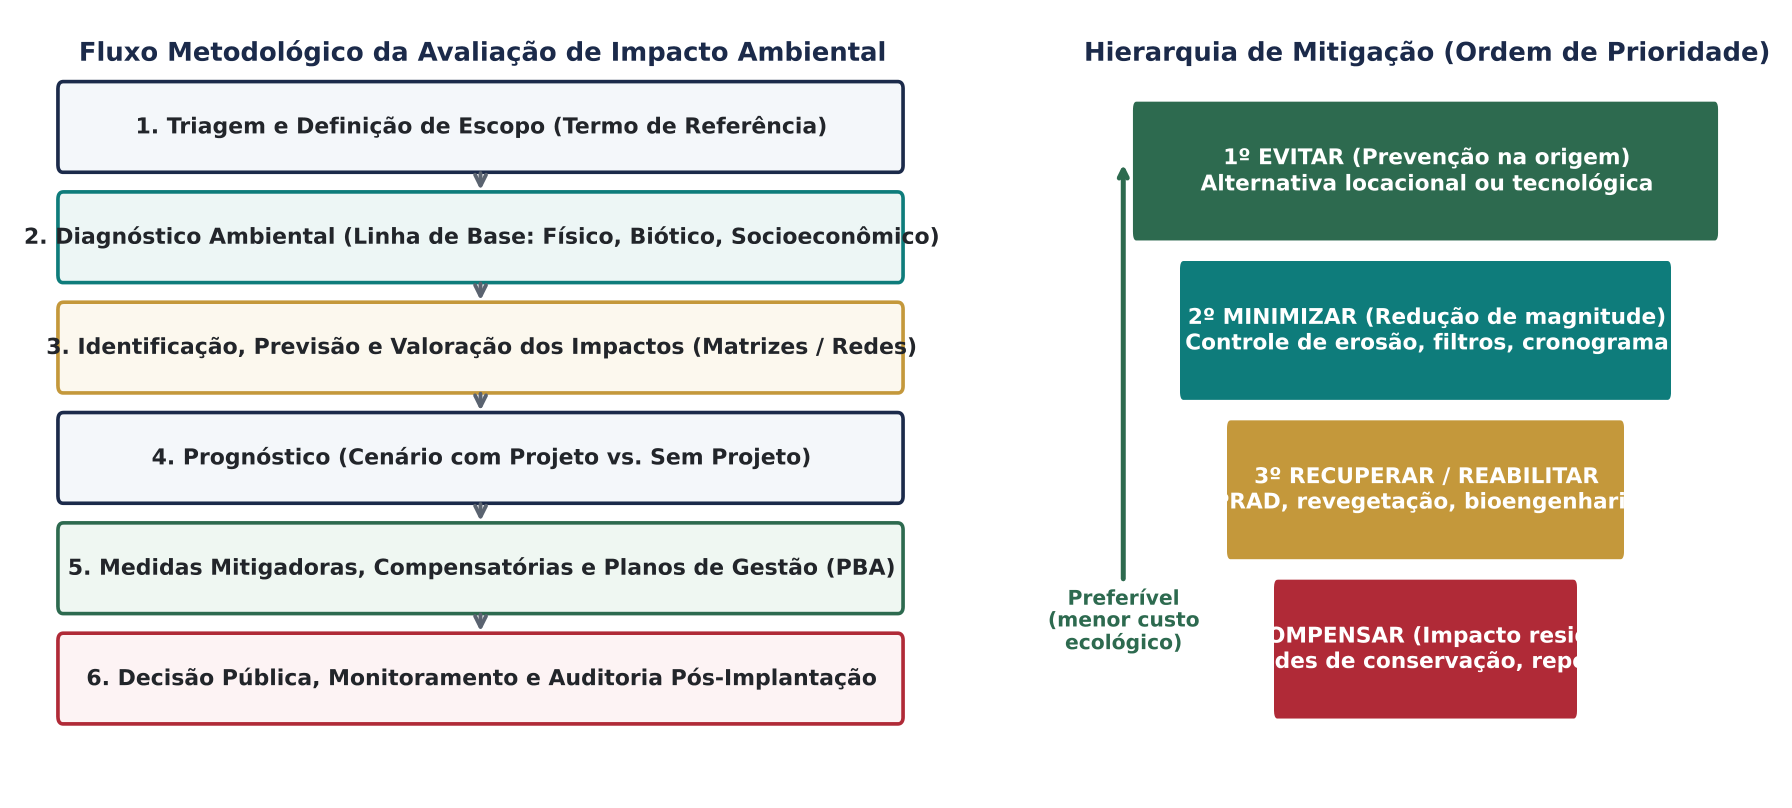
\includegraphics[keepaspectratio]{capitulos/../img/fig03_etapas_aia_mitigacao.png}}

}

\caption{\label{fig-aia_mitigacao}Fluxo metodológico completo da
Avaliação de Impacto Ambiental (Painel A) e ordem de prioridade técnica
da Hierarquia de Mitigação (Painel B). Fonte, elaboração didática da
disciplina CHF662 com base em Sánchez (2013) e Brasil/MMA (2016).}

\end{figure}%

\subsubsection{\texorpdfstring{1. Triagem
(\emph{Screening})}{1. Triagem (Screening)}}\label{triagem-screening}

A triagem responde à primeira pergunta decisória do processo, \emph{este
projeto requer uma AIA completa (EIA/RIMA), um estudo ambiental
simplificado ou está dispensado de AIA?} Os critérios de triagem
combinam a tipologia da atividade (rodovias, parques eólicos, mineração,
barragens), o porte (área, potência, vazão) e, fundamentalmente, a
\textbf{sensibilidade do local} de inserção (proximidade de Unidades de
Conservação, terras indígenas, comunidades tradicionais, nascentes ou
áreas de Caatinga bem conservada).

\subsubsection{\texorpdfstring{2. Definição de Escopo (\emph{Scoping}) e
Termo de Referência
(TR)}{2. Definição de Escopo (Scoping) e Termo de Referência (TR)}}\label{definiuxe7uxe3o-de-escopo-scoping-e-termo-de-referuxeancia-tr}

Confirmada a necessidade de AIA, a definição de escopo delimita \emph{o
que realmente importa estudar}, evitando dois extremos prejudiciais,
relatórios enciclopédicos cheios de dados irrelevantes ou estudos
omissos em impactos críticos. O produto formal dessa etapa é o
\textbf{Termo de Referência (TR)}, emitido pelo órgão ambiental (como o
INEMA na Bahia ou o IBAMA na esfera federal), que especifica a
profundidade do diagnóstico, as metodologias obrigatórias, o horizonte
temporal e as questões levantadas em consultas preliminares.

\subsubsection{3. Diagnóstico Ambiental (Linha de Base) e Áreas de
Influência}\label{diagnuxf3stico-ambiental-linha-de-base-e-uxe1reas-de-influuxeancia}

O diagnóstico constrói a \textbf{linha de base (\emph{baseline})}, ou
seja, o retrato qualiquantitativo do ambiente \emph{antes} da
implantação do projeto, estruturado em três meios interdependentes,

\textbf{Meio físico.} Clima, geologia, geomorfologia, solos, recursos
hídricos superficiais e subterrâneos, qualidade do ar e ruído de fundo;.
\textbf{Meio biótico.} Fitofisionomias, flora (espécies endêmicas ou
ameaçadas), fauna terrestre e aquática, corredores ecológicos e áreas
prioritárias para conservação;. \textbf{Meio socioeconômico.}
Demografia, uso e ocupação da terra, estrutura produtiva, infraestrutura
pública, comunidades quilombolas/indígenas/fundo de pasto e patrimônio
arqueológico e cultural.

O diagnóstico exige a delimitação cartográfica rigorosa das três
\textbf{Áreas de Influência}, que não são círculos arbitrários traçados
com compasso, mas recortes baseados em processos físicos, ecológicos e
sociais reais (microbacias, plumas de dispersão, limites municipais),

{\def\LTcaptype{none} % do not increment counter
\begin{longtable}[]{@{}
  >{\raggedright\arraybackslash}p{(\linewidth - 4\tabcolsep) * \real{0.3333}}
  >{\raggedright\arraybackslash}p{(\linewidth - 4\tabcolsep) * \real{0.3333}}
  >{\raggedright\arraybackslash}p{(\linewidth - 4\tabcolsep) * \real{0.3333}}@{}}
\toprule\noalign{}
\begin{minipage}[b]{\linewidth}\raggedright
\textbf{Área}
\end{minipage} & \begin{minipage}[b]{\linewidth}\raggedright
\textbf{Critério técnico de delimitação}
\end{minipage} & \begin{minipage}[b]{\linewidth}\raggedright
\textbf{Exemplo no Semiárido baiano}
\end{minipage} \\
\midrule\noalign{}
\endhead
\bottomrule\noalign{}
\endlastfoot
\textbf{ADA} (Área Diretamente Afetada) & Superfície efetivamente
ocupada pelas estruturas físicas do empreendimento, canteiros, estradas
de acesso, jazidas e áreas de bota-fora. & Poligonal das bases das
torres eólicas, subestação, linhas internas e vias de acesso abertas na
Caatinga. \\
\textbf{AID} (Área de Influência Direta) & Espaço que sofre impactos
diretos (primários) decorrentes da implantação e operação, geralmente
definido pela microbacia, mancha de ruído ou raio de dispersão de
poeira/fauna. & Microbacia drenada pelos acessos do parque eólico, áreas
de afugentamento de avifauna e povoados lindeiros sujeitos a poeira e
ruído. \\
\textbf{AII} (Área de Influência Indireta) & Espaço alcançado por
impactos secundários ou indiretos (econômicos, demográficos, viários ou
sobre a bacia hidrográfica regional). & Municípios afetados pelo aumento
de arrecadação, demanda por serviços urbanos, tráfego pesado e sub-bacia
regional. \\
\end{longtable}
}

\subsubsection{4. Identificação, Previsão e Valoração de
Impactos}\label{identificauxe7uxe3o-previsuxe3o-e-valorauxe7uxe3o-de-impactos}

Nesta etapa, cruzam-se as ações do projeto (nas fases de planejamento,
implantação, operação e desativação) com os fatores ambientais descritos
no diagnóstico. Os impactos são classificados segundo atributos
padronizados, \textbf{natureza} (adverso ou benéfico),
\textbf{incidência} (direto ou indireto), \textbf{abrangência} (local,
regional ou estratégica), \textbf{temporalidade} (imediato, médio ou
longo prazo), \textbf{duração} (temporário, permanente ou cíclico),
\textbf{reversibilidade} (reversível ou irreversível) e
\textbf{cumulatividade/sinergia} (quando se soma ou se amplifica junto a
outros projetos existentes na bacia).

Para executar essa etapa de modo transparente e auditável, a análise
ambiental emprega quatro famílias principais de métodos,

\textbf{Listagens de controle (\emph{Checklists}),} relações
estruturadas de fatores ambientais e potenciais impactos organizados por
tipologia de projeto. Podem ser \emph{simples} (apenas verificam
presença/ausência), \emph{descritivas} (incluem orientações de medição)
ou \emph{escalares/ponderadas} (atribuem notas e pesos). São rápidas e
úteis na triagem e no escopo, porém tendem a ser estáticas e não
explicitam facilmente as relações diretas entre cada ação específica e
cada efeito indireto. \textbf{Matrizes de interação (Matriz de Leopold e
matrizes ponderadas).} Cruzam em tabela bidimensional as \emph{ações do
empreendimento} (colunas) com os \emph{fatores ambientais} (linhas).
Proposta originalmente por Leopold et al.~(1971) com \(100\) ações e
\(88\) fatores (\(8\,800\) células possíveis), a matriz é hoje adaptada
para cada projeto concreto, avaliando cada interação relevante por
sinal, \textbf{magnitude} e \textbf{importância}.

\textbf{Redes de interação (\emph{Networks}),} diagramas em grafo
(fluxogramas causa-efeito) que rastreiam cadeias de impactos, uma ação
inicial gera um \emph{impacto primário} (direto), que desencadeia
\emph{impactos secundários} e \emph{terciários} (indiretos). Exemplo
clássico no Semiárido, abertura de estrada sem drenagem (ação) \(\to\)
exposição do solo e concentração do escoamento (1ª ordem) \(\to\)
sulcos, ravinas e carreamento de sedimentos para o riacho (2ª ordem)
\(\to\) assoreamento do açude comunitário e redução da disponibilidade
hídrica na seca (3ª ordem).

\textbf{Sobreposição de cartas (\emph{Overlay}) e SIG,} derivada do
método clássico de Ian McHarg (1969) e hoje operada em Sistemas de
Informação Geográfica (SIG), consiste em sobrepor camadas
georreferenciadas (declividade, solos, hidrografia, APPs, remanescentes
florestais, áreas urbanas) por meio de álgebra de mapas. É
insubstituível para \textbf{comparar alternativas locacionais} e
explicitar a distribuição espacial dos impactos, embora dependa
diretamente da qualidade e da escala dos dados cartográficos (tema
aprofundado no Capítulo 6).

{\def\LTcaptype{none} % do not increment counter
\begin{longtable}[]{@{}
  >{\raggedright\arraybackslash}p{(\linewidth - 6\tabcolsep) * \real{0.2500}}
  >{\raggedright\arraybackslash}p{(\linewidth - 6\tabcolsep) * \real{0.2500}}
  >{\raggedright\arraybackslash}p{(\linewidth - 6\tabcolsep) * \real{0.2500}}
  >{\raggedright\arraybackslash}p{(\linewidth - 6\tabcolsep) * \real{0.2500}}@{}}
\toprule\noalign{}
\begin{minipage}[b]{\linewidth}\raggedright
\textbf{Método}
\end{minipage} & \begin{minipage}[b]{\linewidth}\raggedright
\textbf{Principal vantagem}
\end{minipage} & \begin{minipage}[b]{\linewidth}\raggedright
\textbf{Principal limitação}
\end{minipage} & \begin{minipage}[b]{\linewidth}\raggedright
\textbf{Uso ideal}
\end{minipage} \\
\midrule\noalign{}
\endhead
\bottomrule\noalign{}
\endlastfoot
\textbf{Checklists} & Rapidez, memória técnica e padronização inicial. &
Estáticos; não mostram encadeamento causa-efeito nem localização. &
Triagem, escopo e auditorias iniciais. \\
\textbf{Matriz de Leopold / Ponderada} & Liga explicitamente cada ação a
cada fator e permite hierarquizar prioridades. & Dificuldade em
representar impactos indiretos (2ª/3ª ordem) e subjetividade se os
critérios de nota não forem explícitos. & Síntese técnica de EIAs, PCAs
e comparação de ações. \\
\textbf{Redes de Interação} & Evidencia impactos indiretos, cumulativos
e efeitos em cascata nos sistemas naturais. & Pode tornar-se visualmente
complexa em grandes projetos; não quantifica por si só a distribuição
espacial. & Análise de bacias, erosão, hidrologia e cadeias tróficas. \\
\textbf{Sobreposição / SIG} & Explicita exatamente \emph{onde} ocorrem
os conflitos e orienta alternativas locacionais. & Exige base
cartográfica compatível na escala de detalhe; não substitui a análise de
processos sociais não mapeáveis. & Escolha de traçados, parques
energéticos e zoneamentos. \\
\end{longtable}
}

\subsection{Matriz de Leopold Ponderada, Pontuação de Magnitude,
Importância e
Balanço}\label{matriz-de-leopold-ponderada-pontuauxe7uxe3o-de-magnitude-importuxe2ncia-e-balanuxe7o}

Em uma matriz de interação ponderada adaptada de Leopold et al.~(1971),
cada célula \((i,j)\) onde há interação efetiva entre o \textbf{fator
ambiental \(i\)} (linha) e a \textbf{ação do empreendimento \(j\)}
(coluna) recebe três atributos explícitos,

\textbf{Sinal (\(s_{ij} \in \{-1, +1\}\)),} \(-1\) para impacto
\emph{adverso} (negativo) e \(+1\) para impacto \emph{benéfico}
(positivo). Se não houver interação, registra-se \(0\) (célula vazia).
\textbf{Magnitude (\(M_{ij} \in \{1, 2, \dots, 10\}\)).} Expressa a
\emph{extensão física, intensidade ou grau de alteração} provocada pela
ação sobre o fator (\(1\) = alteração mínima e pontual; \(10\) =
alteração máxima e extensa). \textbf{Importância
(\(I_{ij} \in \{1, 2, \dots, 10\}\)).} Expressa a \emph{relevância
ecológica, social, funcional ou legal} do fator afetado (\(1\) = baixa
relevância regional/funcional; \(10\) = relevância crítica, como espécie
ameaçada, manancial de abastecimento ou comunidade tradicional).

\textbf{Equações de cálculo passo a passo,}

\[
P_{ij} = s_{ij} \cdot \left(M_{ij} \times I_{ij}\right) \qquad \text{com } P_{ij} \in [-100, +100]
\]

\[
T_j = \sum_{i=1}^{m} P_{ij} \quad (\text{soma da coluna } j\text{: impacto total da ação } j\text{ sobre os } m \text{ fatores})
\]

\[
F_i = \sum_{j=1}^{n} P_{ij} \quad (\text{soma da linha } i\text{: impacto acumulado das } n \text{ ações sobre o fator } i)
\]

\[
B = \sum_{i=1}^{m}\sum_{j=1}^{n} P_{ij} = \sum_{j=1}^{n} T_j = \sum_{i=1}^{m} F_i, \qquad \text{analisado em conjunto com } \Sigma^{-} = \sum_{P_{ij}<0} P_{ij} \text{ e } \Sigma^{+} = \sum_{P_{ij}>0} P_{ij}
\]

\textbf{Demonstração numérica passo a passo (mini-matriz
\(2 \times 2\)).} Considere duas ações (\(A_1\), supressão vegetal em
encosta; \(A_2\), contratação de mão de obra local) e dois fatores
(\(F_1\), solo e suscetibilidade erosiva; \(F_2\), renda familiar).

Célula \((F_1, A_1)\), impacto adverso (\(s=-1\)), alta intensidade
física (\(M=8\)) em solo frágil de encosta (\(I=9\))
\(\implies P_{11} = -1 \times (8 \times 9) = -72\). Célula
\((F_2, A_1)\), pequeno efeito positivo temporário de pagamento pela
limpeza (\(s=+1\), \(M=2\), \(I=3\))
\(\implies P_{21} = +1 \times (2 \times 3) = +6\). Célula
\((F_1, A_2)\), a contratação em si não altera fisicamente o solo
\(\implies P_{12} = 0\). Célula \((F_2, A_2)\), impacto benéfico
relevante (\(s=+1\), \(M=6\), \(I=7\))
\(\implies P_{22} = +1 \times (6 \times 7) = +42\). \textbf{Somas das
ações (colunas),} \(T_1 = -72 + 6 = -66\) (ação fortemente adversa);
\(T_2 = 0 + 42 = +42\). \textbf{Somas dos fatores (linhas),}
\(F_1 = -72 + 0 = -72\) (fator crítico que exige mitigação prioritária);
\(F_2 = +6 + 42 = +48\).

\textbf{Balanço e alerta metodológico,} \(\Sigma^{-} = -72\),
\(\Sigma^{+} = +48\) e balanço líquido \(B = -72 + 48 = -24\).
\emph{Atenção,} a soma positiva em renda (\(+48\)) \textbf{nunca}
elimina fisicamente a erosão do solo (\(-72\)); por isso, a decisão
técnica exige analisar sempre \(\Sigma^{-}\), \(\Sigma^{+}\) e as
células críticas individuais, nunca apenas o saldo líquido \(B\).

\subsubsection{5. Prognóstico Ambiental, Cenário com Projeto vs.~Cenário
sem
Projeto}\label{prognuxf3stico-ambiental-cenuxe1rio-com-projeto-vs.-cenuxe1rio-sem-projeto}

O prognóstico projeta a evolução futura da qualidade ambiental em dois
cenários comparativos obrigatórios,

\textbf{Cenário sem projeto (alternativa zero).} Não significa um
ambiente congelado no tempo! Mesmo sem o empreendimento, a área continua
evoluindo segundo tendências já instaladas (expansão urbana,
sobrepastejo, mudanças climáticas ou regeneração natural).
\textbf{Cenário com projeto.} Projeta a trajetória ambiental
incorporando o empreendimento, primeiro \emph{sem medidas mitigadoras}
(para revelar a real magnitude potencial do risco) e depois \emph{com as
medidas mitigadoras e de controle propostas} (revelando o impacto
residual).

O impacto verdadeiro atribuível ao projeto corresponde à
\textbf{diferença entre a trajetória futura com o projeto e a trajetória
futura sem o projeto}, e não simplesmente à diferença entre o ``depois''
e o ``antes'' estático.

\subsubsection{6. Hierarquia de Mitigação, Medidas Mitigadoras e
Compensatórias}\label{hierarquia-de-mitigauxe7uxe3o-medidas-mitigadoras-e-compensatuxf3rias}

Diante dos impactos adversos identificados, o planejador ambiental não
pode escolher medidas aleatoriamente ou propor compensação financeira de
imediato para danos que poderiam ser evitados. A prática internacional e
a legislação ambiental impõem a \textbf{Hierarquia de Mitigação},
representada no Painel B da Figura~\ref{fig-aia_mitigacao},

\textbf{1º, Evitar (prevenção na origem).} Alterar a localização, o
traçado, o cronograma ou a tecnologia do projeto para impedir que o
impacto sequer ocorra. É o degrau de maior eficácia ecológica e,
frequentemente, de menor custo global a longo prazo. \textbf{2º,
Minimizar (redução de magnitude, duração ou extensão).} Quando o impacto
não pode ser integralmente evitado, aplicam-se controles de engenharia e
manejo para reduzir sua intensidade (filtros, bacias de contenção de
sedimentos, supressão seletiva, limitação de horários de tráfego).

\textbf{3º, Recuperar / Reabilitar (restauração \emph{in situ}),} após a
intervenção temporária (como canteiros de obra, taludes de corte e áreas
de empréstimo), restabelecem-se as funções do solo, da drenagem e da
cobertura vegetal por meio de Plano de Recuperação de Áreas Degradadas
(PRAD) e técnicas de bioengenharia. \textbf{4º, Compensar (último
recurso, apenas para o impacto residual).} Aplica-se estritamente à
fração de dano inevitável que permanece após esgotados os três degraus
anteriores. Exemplos, apoio à criação ou consolidação de Unidades de
Conservação (art. 36 da Lei nº 9.985/2000, Sistema Nacional de Unidades
de Conservação da Natureza, SNUC), reposição florestal equivalente ou
superior em área e qualidade ecológica (\emph{offset} de biodiversidade)
e programas de fortalecimento comunitário.

Para impactos \textbf{benéficos}, em vez de medidas mitigadoras,
formulam-se \textbf{medidas potencializadoras} (por exemplo, capacitação
profissional prévia de moradores locais para maximizar a absorção de mão
de obra da AID).

\subsubsection{7. Plano Básico Ambiental (PBA) e Monitoramento
Pós-Implantação}\label{plano-buxe1sico-ambiental-pba-e-monitoramento-puxf3s-implantauxe7uxe3o}

Na etapa de decisão, o órgão ambiental emite parecer técnico e decide
pelo deferimento (com condicionantes) ou indeferimento da licença
(Licença Prévia {[}LP{]}, seguida de Licença de Instalação {[}LI{]} e
Licença de Operação {[}LO{]}). Os compromissos genéricos listados no EIA
são então detalhados em projetos executivos no \textbf{Plano Básico
Ambiental (PBA)}, que reúne programas operacionais como, Programa de
Controle de Processos Erosivos, Programa de Monitoramento da Qualidade
da Água, Programa de Resgate e Monitoramento de Fauna, Programa de
Educação Ambiental e PRAD.

O \textbf{monitoramento pós-implantação} (acompanhamento) fecha o ciclo
da AIA. Medindo periodicamente os mesmos indicadores levantados na linha
de base (turbidez da água, taxa de erosão, ruído, sobrevivência de
mudas), o monitoramento verifica se as previsões do estudo estavam
corretas e se as medidas do PBA atingiram as metas estipuladas. Caso os
indicadores ultrapassem os limites toleráveis, aciona-se a
\textbf{gestão adaptativa}, com correção imediata dos controles em
campo.

\subsection{Diagnóstico, cenário de referência e efeitos
cumulativos}\label{diagnuxf3stico-cenuxe1rio-de-referuxeancia-e-efeitos-cumulativos}

O cenário de referência descreve a trajetória provável do ambiente
durante o período analisado, considerando tendências já existentes. A
comparação com o empreendimento deve manter o mesmo horizonte temporal.
Uma área submetida a expansão urbana pode apresentar mudanças mesmo sem
o projeto proposto, o que exige distinguir tendências preexistentes e
efeitos adicionais.

Impactos cumulativos surgem quando pressões de diferentes atividades se
combinam sobre um receptor. Estradas de parques vizinhos podem
direcionar água para o mesmo riacho, enquanto captações de usuários
distintos afetam a disponibilidade hídrica de um mesmo trecho. A análise
precisa definir o receptor, a extensão espacial e o período de
acumulação para que o efeito possa ser investigado.

Uma matriz ponderada auxilia a comparação quando critérios e pesos são
transparentes. A soma de notas perde poder explicativo se os impactos
mais relevantes forem compensados numericamente por benefícios sem
relação funcional com eles. A decisão deve apresentar os resultados por
componente, reconhecer restrições e comparar alternativas de
localização, tecnologia e operação.

O acompanhamento completa a análise ao confrontar previsão e observação.
Uma medida de controle precisa de condição inicial, meta, frequência de
verificação e responsável. A mudança observada deve ser interpretada
junto às condições de chuva, operação e manutenção, permitindo corrigir
a intervenção quando o resultado divergir do esperado.

\section{Etapa 4 - Exemplos
resolvidos}\label{etapa-4---exemplos-resolvidos-4}

\subsection{Exemplo 5.1 - Delimitação Quantitativa de ADA, AID e AII em
Parque Solar no Semiárido (Nível
Básico)}\label{exemplo-5.1---delimitauxe7uxe3o-quantitativa-de-ada-aid-e-aii-em-parque-solar-no-semiuxe1rido-nuxedvel-buxe1sico}

\textbf{Situação analisada.} Uma empresa propõe a instalação de uma
usina solar fotovoltaica em área rural de transição semiárida na Bahia.
O projeto prevê \(45{,}0\,\text{ha}\) ocupados pelos arranjos de painéis
solares, mais \(3{,}5\,\text{ha}\) destinados à subestação, canteiro de
obras e estradas internas de acesso. A microbacia hidrográfica que drena
o empreendimento possui \(620{,}0\,\text{ha}\), e o município de
inserção ocupa \(48\,500{,}0\,\text{ha}\).

\textbf{Dados disponíveis.} Área dos painéis \(= 45{,}0\,\text{ha}\);
áreas de apoio e acessos \(= 3{,}5\,\text{ha}\); área da microbacia (AID
do meio físico) \(= 620{,}0\,\text{ha}\); área do município (AII
socioeconômica) \(= 48\,500{,}0\,\text{ha}\).

\textbf{Problema a resolver.} Calcular a Área Diretamente Afetada (ADA)
total, determinar o percentual que a ADA representa em relação à AID e à
AII, e justificar por que a AID do meio físico deve acompanhar os
divisores da microbacia e não um círculo arbitrário.

\textbf{Fundamento da análise.} Soma das superfícies de intervenção
direta para obtenção da ADA e cálculo de razão percentual
(\(\text{ADA}/\text{AID} \times 100\%\) e
\(\text{ADA}/\text{AII} \times 100\%\)), articulados aos critérios
físicos de delimitação de áreas de influência em AIA (Sánchez, 2013).

\textbf{Desenvolvimento.}

\textbf{Cálculo da ADA.} Somam-se todas as áreas com supressão ou
ocupação direta pelas estruturas principais e auxiliares,

\[
\text{ADA} = 45{,}0 + 3{,}5 = 48{,}5\,\text{ha}.
\]

. \textbf{Proporção da ADA na AID (microbacia),}

\[
\frac{\text{ADA}}{\text{AID}} \times 100\% = \frac{48{,}5}{620{,}0} \times 100\% = 0{,}078225\dots \times 100\% \approx 7{,}82\%.
\]

. \textbf{Proporção da ADA na AII (município),}

\[
\frac{\text{ADA}}{\text{AII}} \times 100\% = \frac{48{,}5}{48\,500{,}0} \times 100\% = 0{,}001 \times 100\% = 0{,}10\%.
\]

. \textbf{Critério físico da AID.} O escoamento superficial, o
carreamento de sedimentos e eventuais vazamentos de óleos de
transformadores obedecem à gravidade e aos divisores topográficos. Um
círculo fixo de \(1\,\text{km}\) incluiria trechos de bacias vizinhas
sem conexão hídrica com o parque e deixaria de fora o exutório a jusante
que efetivamente receberá os sedimentos.

\textbf{Interpretação do resultado.} \(\text{ADA} = 48{,}5\,\text{ha}\),
correspondendo a \(7{,}82\%\) da AID (microbacia) e \(0{,}10\%\) da AII
(município). A AID física deve coincidir com a microbacia porque os
fluxos hidrossedimentológicos seguem a drenagem natural.

\textbf{Condições de validade.} O resultado é coerente,
\(\text{ADA} < \text{AID} < \text{AII}\)
(\(48{,}5 < 620{,}0 < 48\,500{,}0\,\text{ha}\)). Note também um alerta
importante de análise ambiental, embora \(0{,}10\%\) do município pareça
desprezível na escala da AII, ocupar \(7{,}82\%\) da microbacia local
com superfícies compactadas e painéis já é suficiente para alterar o
pico de escoamento superficial local se não houver drenagem e proteção
do solo adequadas.

\subsection{Exemplo 5.2 - Matriz de Leopold Ponderada em Parque Eólico
na Caatinga (Nível
Básico-Intermediário)}\label{05-avaliacao-impacto-ambiental-exemplo-5.2.-matriz-de-leopold-ponderada-em-parque-euxf3lico-na-caatinga-nuxedvel-buxe1sicointermediuxe1rio}

\textbf{Situação analisada.} Durante a AIA de um parque eólico no
Semiárido baiano, a equipe técnica construiu uma matriz simplificada
cruzando três ações principais (\(A_1\), supressão vegetal e abertura de
acessos; \(A_2\), escavação e concretagem das fundações das torres;
\(A_3\), operação dos aerogeradores e contratação de serviços locais)
com quatro fatores ambientais (\(F_1\), solo e processos erosivos;
\(F_2\), fauna e avifauna; \(F_3\), qualidade da água superficial;
\(F_4\), emprego e renda local).

\textbf{Dados disponíveis.} Avaliações \((s, M, I)\) atribuídas por
célula após vistorias de campo e consulta à linha de base,

\(F_1\) (Solo/Erosão), \(A_1 = (-, 8, 9)\); \(A_2 = (-, 6, 8)\);
\(A_3 = 0\). \(F_2\) (Fauna/Avifauna), \(A_1 = (-, 7, 8)\);
\(A_2 = (-, 3, 5)\); \(A_3 = (-, 5, 9)\). \(F_3\) (Qualidade da água),
\(A_1 = (-, 5, 7)\); \(A_2 = (-, 4, 7)\); \(A_3 = 0\). \(F_4\)
(Emprego/Renda), \(A_1 = (+, 3, 5)\); \(A_2 = (+, 4, 5)\);
\(A_3 = (+, 7, 8)\).

\textbf{Problema a resolver.} Calcular todas as pontuações celulares
\(P_{ij}\), os totais por ação (\(T_j\)), os totais por fator (\(F_i\)),
a carga adversa (\(\Sigma^{-}\)), a carga benéfica (\(\Sigma^{+}\)) e o
balanço líquido (\(B\)), identificando a ação mais crítica e o fator
mais impactado.

\textbf{Fundamento da análise.} Aplicação direta das equações da Matriz
de Leopold Ponderada, \(P_{ij} = s_{ij} \cdot (M_{ij} \times I_{ij})\),
com verificação cruzada pela igualdade \(\sum T_j = \sum F_i = B\).

\textbf{Desenvolvimento.}

Linha \(F_1\), \(P_{11} = -(8 \times 9) = -72\);
\(P_{12} = -(6 \times 8) = -48\); \(P_{13} = 0\). Linha \(F_2\),
\(P_{21} = -(7 \times 8) = -56\); \(P_{22} = -(3 \times 5) = -15\);
\(P_{23} = -(5 \times 9) = -45\). Linha \(F_3\),
\(P_{31} = -(5 \times 7) = -35\); \(P_{32} = -(4 \times 7) = -28\);
\(P_{33} = 0\). Linha \(F_4\), \(P_{41} = +(3 \times 5) = +15\);
\(P_{42} = +(4 \times 5) = +20\); \(P_{43} = +(7 \times 8) = +56\).

\textbf{Cálculo de cada célula \(P_{ij}\),}. \textbf{Montagem da tabela
e somas por linha (\(F_i\)) e por coluna (\(T_j\)),}.

{\def\LTcaptype{none} % do not increment counter
\begin{longtable}[]{@{}
  >{\raggedright\arraybackslash}p{(\linewidth - 8\tabcolsep) * \real{0.2000}}
  >{\raggedright\arraybackslash}p{(\linewidth - 8\tabcolsep) * \real{0.2000}}
  >{\raggedright\arraybackslash}p{(\linewidth - 8\tabcolsep) * \real{0.2000}}
  >{\raggedright\arraybackslash}p{(\linewidth - 8\tabcolsep) * \real{0.2000}}
  >{\raggedright\arraybackslash}p{(\linewidth - 8\tabcolsep) * \real{0.2000}}@{}}
\toprule\noalign{}
\begin{minipage}[b]{\linewidth}\raggedright
\textbf{Fator Ambiental}
\end{minipage} & \begin{minipage}[b]{\linewidth}\raggedright
\textbf{\(A_1\) (Acessos)}
\end{minipage} & \begin{minipage}[b]{\linewidth}\raggedright
\textbf{\(A_2\) (Fundações)}
\end{minipage} & \begin{minipage}[b]{\linewidth}\raggedright
\textbf{\(A_3\) (Operação)}
\end{minipage} & \begin{minipage}[b]{\linewidth}\raggedright
\textbf{Total \(F_i\)}
\end{minipage} \\
\midrule\noalign{}
\endhead
\bottomrule\noalign{}
\endlastfoot
\(F_1\), Solo / Erosão & \(-72\) & \(-48\) & \(0\) &
\(\mathbf{-120}\) \\
\(F_2\), Fauna / Avifauna & \(-56\) & \(-15\) & \(-45\) &
\(\mathbf{-116}\) \\
\(F_3\), Qualidade da água & \(-35\) & \(-28\) & \(0\) &
\(\mathbf{-63}\) \\
\(F_4\), Emprego / Renda & \(+15\) & \(+20\) & \(+56\) &
\(\mathbf{+91}\) \\
\textbf{Total da Ação (\(T_j\))} & \(\mathbf{-148}\) & \(\mathbf{-71}\)
& \(\mathbf{+11}\) & \(\mathbf{B = -208}\) \\
\end{longtable}
}

\textbf{Conferência das somas por linha e por coluna,}

\[
\begin{aligned}
\sum F_i &= (-120) + (-116) + (-63) + 91 = -299 + 91 = -208, \\
\sum T_j &= (-148) + (-71) + 11 = -219 + 11 = -208.
\end{aligned}
\]

. \textbf{Separação de cargas adversa e benéfica,}

\[
\Sigma^{-} = -72 - 48 - 56 - 15 - 45 - 35 - 28 = -299, \qquad \Sigma^{+} = +15 + 20 + 56 = +91.
\]

.

\textbf{Interpretação do resultado.} A ação mais impactante
negativamente é \(A_1\) (supressão e acessos, \(T_1 = -148\)) e o fator
mais vulnerável é \(F_1\) (solo/erosão, \(F_1 = -120\)), seguido de
perto por \(F_2\) (fauna/avifauna, \(F_2 = -116\)). A carga adversa
total é \(\Sigma^{-} = -299\), a carga benéfica é \(\Sigma^{+} = +91\) e
o balanço líquido é \(B = -208\).

\textbf{Condições de validade.} A igualdade
\(\sum F_i = \sum T_j = \Sigma^{-} + \Sigma^{+} = -208\) confirma a
exatidão aritmética. Do ponto de vista ambiental, observe a célula
\(P_{23} = -45\) (colisão de avifauna na operação), mesmo com
\(T_3 = +11\) (saldo positivo na coluna \(A_3\)), o impacto sobre aves
ameaçadas da Caatinga (como a arara-azul-de-lear na região de Canudos)
tem importância \(I = 9\) e exige monitoramento e sistemas de
desligamento preventivo, nunca podendo ser mascarado pelos \(+56\)
pontos de renda.

\subsection{Exemplo 5.3 - Prognóstico e Seleção Multicritério de
Alternativas Locacionais (Nível
Intermediário)}\label{exemplo-5.3---prognuxf3stico-e-seleuxe7uxe3o-multicrituxe9rio-de-alternativas-locacionais-nuxedvel-intermediuxe1rio}

\textbf{Situação analisada.} No estudo de duplicação de uma rodovia
estadual na Bahia, o EIA comparou duas alternativas locacionais diante
do cenário sem projeto, o \textbf{Traçado A} (mais curto, porém
atravessa uma APP de nascente e um fragmento contínuo de Caatinga) e o
\textbf{Traçado B} (\(1{,}2\,\text{km}\) mais extenso, contornando a APP
por áreas já antropizadas de pastagem).

\textbf{Dados disponíveis.} Quatro critérios ponderados (soma dos pesos
\(= 1{,}00\)) avaliados em escala de \textbf{severidade adversa} de
\(0\) (nenhum dano) a \(10\) (dano máximo),

\(C_1\), Supressão de APP e vegetação nativa (peso \(w_1 = 0{,}35\)),
Traçado A \(= 9\); Traçado B \(= 3\). \(C_2\), Risco erosivo e
assoreamento de drenagem (peso \(w_2 = 0{,}30\)), Traçado A \(= 8\);
Traçado B \(= 4\). \(C_3\), Fragmentação e atropelamento de fauna (peso
\(w_3 = 0{,}20\)), Traçado A \(= 8\); Traçado B \(= 4\). \(C_4\), Custo
financeiro e extensão adicional da obra (peso \(w_4 = 0{,}15\)), Traçado
A \(= 4\); Traçado B \(= 7\).

\textbf{Problema a resolver.} Calcular o Índice de Impacto Adverso
Ponderado (\(I_{\text{adv}}\)) de cada alternativa, a redução percentual
de impacto adverso ao optar pelo melhor traçado e explicar em qual
degrau da Hierarquia de Mitigação essa escolha se enquadra.

\textbf{Fundamento da análise.} Cálculo da média ponderada
\(I_{\text{adv}} = \sum_{k=1}^{4} w_k \cdot C_k\), seguida de variação
percentual relativa \((I_A - I_B)/I_A \times 100\%\).

\textbf{Desenvolvimento.}

\textbf{Verificação dos pesos,}
\(0{,}35 + 0{,}30 + 0{,}20 + 0{,}15 = 1{,}00\) (normalização correta).
\textbf{Índice adverso do Traçado A (\(I_A\)),}

\[
\begin{aligned}
I_A &= (0{,}35 \times 9) + (0{,}30 \times 8) + (0{,}20 \times 8) + (0{,}15 \times 4) \\
&= 3{,}15 + 2{,}40 + 1{,}60 + 0{,}60 = 7{,}75.
\end{aligned}
\]

. \textbf{Índice adverso do Traçado B (\(I_B\)),}

\[
\begin{aligned}
I_B &= (0{,}35 \times 3) + (0{,}30 \times 4) + (0{,}20 \times 4) + (0{,}15 \times 7) \\
&= 1{,}05 + 1{,}20 + 0{,}80 + 1{,}05 = 4{,}10.
\end{aligned}
\]

. \textbf{Redução percentual da severidade adversa (A para B),}

\[
\text{Redução} = \frac{7{,}75 - 4{,}10}{7{,}75} \times 100\% = \frac{3{,}65}{7{,}75} \times 100\% \approx 47{,}10\%.
\]

.

\textbf{Interpretação do resultado.} O Traçado B é tecnicamente superior
(\(I_B = 4{,}10\) contra \(I_A = 7{,}75\)), promovendo redução de
\(47{,}10\%\) no índice de severidade adversa. Trata-se de uma medida do
1º degrau da Hierarquia de Mitigação (\textbf{Evitar}), via alternativa
locacional.

\textbf{Condições de validade.} Como a escala avalia severidade adversa,
o menor valor indica o melhor desempenho. Apesar de o Traçado B ter nota
pior no critério financeiro (\(7\) contra \(4\)), o ganho ambiental em
APP, erosão e fauna reduz quase pela metade o dano global e evita custos
elevados com licenciamento em APP, obras emergenciais contra erosão e
compensações futuras.

\subsection{Exemplo 5.4 - Aplicação Sequencial da Hierarquia de
Mitigação em Loteamento Periurbano (Nível
Intermediário-Avançado)}\label{05-avaliacao-impacto-ambiental-exemplo-5.4.-aplicauxe7uxe3o-sequencial-da-hierarquia-de-mitigauxe7uxe3o-em-loteamento-periurbano-nuxedvel-intermediuxe1rioavanuxe7ado}

\textbf{Situação analisada.} O anteprojeto de um loteamento periurbano
previa inicialmente a supressão de \(12{,}0\,\text{ha}\) de vegetação
nativa e um aporte estimado de \(480{,}0\,\text{t/ano}\) de sedimentos
para um riacho a jusante. Após revisão pela equipe de Análise Ambiental,
aplicaram-se sequencialmente os quatro degraus da Hierarquia de
Mitigação.

\textbf{Dados disponíveis.}

\textbf{1º Evitar.} Revisão do desenho urbanístico (exclusão de quadras
nas encostas mais declivosas) evita \(45\%\) da supressão vegetal
inicial e \(45\%\) do aporte de sedimentos. \textbf{2º Minimizar.}
Técnicas de supressão seletiva poupam mais \(1{,}6\,\text{ha}\) de mata;
bacias de contenção e proteção provisória do solo retêm \(60\%\) do
sedimento restante. \textbf{3º Recuperar.} Revegetação e bioengenharia
recuperam \(2{,}0\,\text{ha}\) de áreas temporárias (canteiros e
taludes) e reduzem em \(75\%\) o sedimento remanescente. \textbf{4º
Compensar.} O órgão ambiental exige compensação ecológica na razão
\(2:1\) (dois hectares conservados ou restaurados para cada hectare de
perda permanente residual).

\textbf{Problema a resolver.} Calcular, em cada degrau, a área de
vegetação afetada remanescente, o aporte remanescente de sedimentos, o
percentual total de abatimento de sedimentos e a área exata de
compensação ecológica exigida no 4º degrau.

\textbf{Fundamento da análise.} Abatimento sequencial (em cascata) sobre
o saldo remanescente de cada degrau, sem somar percentuais diretamente
sobre a base inicial quando aplicados a etapas sucessivas.

\textbf{Desenvolvimento.} \textbf{A. Trajetória da supressão vegetal
(ha),}

\textbf{Evitar (\(45\%\) de \(12{,}0\,\text{ha}\)).} Área evitada
\(= 0{,}45 \times 12{,}0 = 5{,}4\,\text{ha}\). Saldo após degrau 1
\(= 12{,}0 - 5{,}4 = 6{,}6\,\text{ha}\). \textbf{Minimizar (corte
seletivo de \(1{,}6\,\text{ha}\)).} Saldo após degrau 2
\(= 6{,}6 - 1{,}6 = 5{,}0\,\text{ha}\). \textbf{Recuperar
(\(2{,}0\,\text{ha}\) temporários restaurados \emph{in situ}),} perda
permanente residual \(= 5{,}0 - 2{,}0 = 3{,}0\,\text{ha}\).
\textbf{Compensar (razão \(2:1\) sobre o impacto residual).} Área a
compensar \(= 2 \times 3{,}0 = 6{,}0\,\text{ha}\).

\textbf{B. Trajetória do aporte de sedimentos (\(\text{t/ano}\)),}

\textbf{Evitar (\(45\%\) de \(480{,}0\)).} Evitados
\(= 0{,}45 \times 480{,}0 = 216{,}0\,\text{t/ano}\). Saldo 1
\(= 480{,}0 - 216{,}0 = 264{,}0\,\text{t/ano}\). \textbf{Minimizar
(\(60\%\) do saldo 1).} Retidos
\(= 0{,}60 \times 264{,}0 = 158{,}4\,\text{t/ano}\). Saldo 2
\(= 264{,}0 - 158{,}4 = 105{,}6\,\text{t/ano}\). \textbf{Recuperar
(\(75\%\) do saldo 2).} Retidos
\(= 0{,}75 \times 105{,}6 = 79{,}2\,\text{t/ano}\). Impacto residual
\(= 105{,}6 - 79{,}2 = 26{,}4\,\text{t/ano}\). \textbf{Redução
percentual acumulada de sedimentos,}

\[
\text{Redução total} = \frac{480{,}0 - 26{,}4}{480{,}0} \times 100\% = \frac{453{,}6}{480{,}0} \times 100\% = 94{,}50\%.
\]

.

\textbf{Interpretação do resultado.} Após a aplicação da Hierarquia de
Mitigação, o impacto residual permanente cai para \(3{,}0\,\text{ha}\)
de vegetação (exigindo \(6{,}0\,\text{ha}\) de compensação na razão
\(2:1\)) e para \(26{,}4\,\text{t/ano}\) de sedimentos (abatimento total
de \(94{,}50\%\)).

\textbf{Condições de validade.} Confere-se a multiplicação em cascata
para sedimentos,
\(480{,}0 \times (1 - 0{,}45) \times (1 - 0{,}60) \times (1 - 0{,}75) = 480{,}0 \times 0{,}55 \times 0{,}40 \times 0{,}25 = 480{,}0 \times 0{,}055 = 26{,}4\,\text{t/ano}\).
Sem a hierarquia, tentar ``compensar'' diretamente os
\(12{,}0\,\text{ha}\) exigiria \(24{,}0\,\text{ha}\) de reposição e
ainda deixaria o riacho assoreado com \(480\,\text{t/ano}\) de
sedimentos.

\subsection{Exemplo 5.5 - Auditoria de Eficiência no Monitoramento
Pós-Implantação do PBA (Nível
Avançado)}\label{exemplo-5.5---auditoria-de-eficiuxeancia-no-monitoramento-puxf3s-implantauxe7uxe3o-do-pba-nuxedvel-avanuxe7ado}

\textbf{Situação analisada.} Durante a construção de uma barragem de
regularização hídrica no rio Jacuípe (Bahia), o diagnóstico da linha de
base registrou turbidez média de \(18{,}0\,\text{NTU}\) a jusante do
eixo barrável em período de estiagem. Nas primeiras semanas de
terraplenagem sem controle, a turbidez saltou para
\(112{,}0\,\text{NTU}\). Acionado o Programa de Controle de Sedimentos
do PBA (instalação de cortinas de siltagem e diques de contenção), o
monitoramento subsequente mediu \(33{,}0\,\text{NTU}\). A condicionante
da Licença de Instalação estabelecia limite máximo operacional de
\(40{,}0\,\text{NTU}\).

\textbf{Dados disponíveis.} Turbidez de linha de base
\(T_0 = 18{,}0\,\text{NTU}\); turbidez sem mitigação
\(T_{\text{sem}} = 112{,}0\,\text{NTU}\); turbidez monitorada com PBA
\(T_{\text{com}} = 33{,}0\,\text{NTU}\); limite da condicionante
\(T_{\max} = 40{,}0\,\text{NTU}\).

\textbf{Problema a resolver.} Calcular o acréscimo de turbidez
atribuível à obra sem mitigação, o acréscimo residual após o PBA, a
eficiência percentual de abatimento do acréscimo antrópico e emitir
parecer técnico sobre o atendimento à condicionante.

\textbf{Fundamento da análise.} Cálculo da anomalia acima da linha de
base (\(\Delta T = T - T_0\)) e da eficiência de mitigação sobre a carga
incremental,
\(E_f = \frac{\Delta T_{\text{sem}} - \Delta T_{\text{com}}}{\Delta T_{\text{sem}}} \times 100\% = \frac{T_{\text{sem}} - T_{\text{com}}}{T_{\text{sem}} - T_0} \times 100\%\).

\textbf{Desenvolvimento.}

\textbf{Acréscimo de turbidez sem mitigação (em relação à linha de
base),}

\[
\Delta T_{\text{sem}} = 112{,}0 - 18{,}0 = 94{,}0\,\text{NTU}.
\]

. \textbf{Acréscimo residual após ativação do PBA,}

\[
\Delta T_{\text{com}} = 33{,}0 - 18{,}0 = 15{,}0\,\text{NTU}.
\]

. \textbf{Parcela efetivamente abatida pelas medidas do PBA,}

\[
\Delta T_{\text{abatida}} = 94{,}0 - 15{,}0 = 79{,}0\,\text{NTU} \quad (\text{ou } 112{,}0 - 33{,}0 = 79{,}0\,\text{NTU}).
\]

. \textbf{Eficiência percentual de abatimento da carga antrópica,}

\[
E_f = \frac{79{,}0}{94{,}0} \times 100\% = 0{,}840425\dots \times 100\% \approx 84{,}04\%.
\]

. \textbf{Verificação da condicionante.} Como
\(33{,}0\,\text{NTU} \le 40{,}0\,\text{NTU}\), a meta legal foi atendida
com folga de \(7{,}0\,\text{NTU}\).

\textbf{Interpretação do resultado.} O acréscimo sem controle foi de
\(94{,}0\,\text{NTU}\), reduzido para um acréscimo residual de
\(15{,}0\,\text{NTU}\) com eficiência de abatimento de \(84{,}04\%\). A
condicionante de \(40{,}0\,\text{NTU}\) está atendida, mas o
monitoramento deve prosseguir continuamente, sobretudo na estação
chuvosa.

\textbf{Condições de validade.} Por que descontar
\(T_0 = 18{,}0\,\text{NTU}\) no denominador? Porque o rio já apresentava
turbidez natural de \(18{,}0\,\text{NTU}\) antes da obra; uma medida de
controle não visa ``zerar'' a turbidez natural do rio, mas abater o
acréscimo provocado pela intervenção. Sem o desconto da linha de base, o
cálculo subestimaria a eficiência real (\(79/112 = 70{,}54\%\)).

\section{Etapa 5 - Erros de
interpretação}\label{etapa-5---erros-de-interpretauxe7uxe3o-4}

\subsection{Erro 1, Confundir AIA com EIA/RIMA ou tratar o licenciamento
como mera
burocracia}\label{erro-1-confundir-aia-com-eiarima-ou-tratar-o-licenciamento-como-mera-burocracia}

\textbf{Equívoco frequente.} Afirmar que ``todo licenciamento exige
EIA/RIMA'' ou usar AIA e EIA como sinônimos exatos.

\textbf{Por que está incorreto.} A AIA é o \emph{processo amplo} de
avaliação prévia de impactos (triagem, escopo, estudos, decisão e
monitoramento), enquanto o EIA/RIMA é apenas uma de suas
\emph{modalidades documentais}, exigida quando há potencial de
\textbf{significativa degradação ambiental}. Projetos de menor potencial
poluidor passam por triagem e apresentam estudos simplificados (como RAS
ou PCA).

\textbf{Como evitar.} Lembre sempre a relação todo-parte, o EIA/RIMA
está contido na AIA, e a AIA integra o planejamento e o licenciamento
ambiental.

\subsection{Erro 2, Somar benefícios econômicos com danos ecológicos
para ``zerar'' o impacto na
Matriz}\label{erro-2-somar-benefuxedcios-econuxf4micos-com-danos-ecoluxf3gicos-para-zerar-o-impacto-na-matriz}

\textbf{Equívoco frequente.} Concluir que um empreendimento é
ambientalmente viável apenas porque a soma algébrica
\(B = \Sigma^{+} + \Sigma^{-}\) ficou próxima de zero ou positiva (por
exemplo, \(+80\) em arrecadação contra \(-75\) em destruição de
nascente).

\textbf{Por que está incorreto.} A pontuação da Matriz de Leopold é
ordinal/semiquantitativa e refere-se a dimensões
\textbf{incomensuráveis}. Gerar empregos temporários não impede o
assoreamento de um manancial nem ressuscita uma espécie endêmica
perdida.

\textbf{Como evitar.} Apresente sempre separadamente \(\Sigma^{-}\),
\(\Sigma^{+}\) e o destaque das células críticas de alta importância
(\(I \ge 8\)) ou irreversíveis, vinculando cada célula adversa a uma
medida concreta da Hierarquia de Mitigação.

\subsection{Erro 3, Inverter a Hierarquia de Mitigação usando a
compensação como ``licença para
degradar''}\label{erro-3-inverter-a-hierarquia-de-mitigauxe7uxe3o-usando-a-compensauxe7uxe3o-como-licenuxe7a-para-degradar}

\textbf{Equívoco frequente.} Propor diretamente compensação financeira
ou plantio em outro município para suprimir uma APP ou um fragmento
florestal sem antes avaliar se outro traçado ou tecnologia evitaria a
perda.

\textbf{Por que está incorreto.} A compensação ocupa o \textbf{4º e
último degrau} da hierarquia, restrita exclusivamente ao \emph{impacto
residual} que não pôde ser evitado, minimizado nem recuperado no local.

\textbf{Como evitar.} Em qualquer diagnóstico ou prova, estruture suas
propostas sempre na sequência obrigatória, \textbf{1º Evitar \(\to\) 2º
Minimizar \(\to\) 3º Recuperar \(\to\) 4º Compensar}.

\subsection{Erro 4, Delimitar ADA, AID e AII como círculos concêntricos
arbitrários sem base
física}\label{erro-4-delimitar-ada-aid-e-aii-como-cuxedrculos-concuxeantricos-arbitruxe1rios-sem-base-fuxedsica}

\textbf{Equívoco frequente.} Traçar raios fixos de \(500\,\text{m}\)
(AID) e \(5\,\text{km}\) (AII) no mapa sem considerar divisores de
bacia, direção dos ventos, rotas de fauna ou malha viária.

\textbf{Por que está incorreto.} Processos ambientais não se propagam
isotropicamente em círculos perfeitos. Um efluente lançado num riacho
percorre quilômetros a jusante seguindo o talvegue, mas não afeta um
ponto a \(200\,\text{m}\) atrás do divisor topográfico.

\textbf{Como evitar.} Delimite a AID do meio físico pela microbacia ou
área de drenagem, a AID biótica pelos habitats e corredores ecológicos
afetados e a AII socioeconômica pela rede de relações territoriais e
municipais.

\section{Etapa 6 - Exercícios de
fixação}\label{etapa-6---exercuxedcios-de-fixauxe7uxe3o-4}

\subsubsection{Nível 1, Básico (Conceitos, Etapas e Cálculos
Fundamentais)}\label{nuxedvel-1-buxe1sico-conceitos-etapas-e-cuxe1lculos-fundamentais}

\begin{enumerate}
\def\labelenumi{\arabic{enumi}.}
\item
  Explique, com base em Sánchez (2013), qual é o papel preventivo da
  Avaliação de Impacto Ambiental (AIA) e por que sua inserção tardia,
  após a definição do projeto de engenharia, compromete sua eficácia no
  planejamento ambiental.
\item
  Em uma matriz de interação ponderada adaptada de Leopold, uma
  atividade de terraplenagem apresentou três interações relevantes,
  solo/erosão \((-, M=7, I=8)\); qualidade do ar por poeira
  \((-, M=4, I=6)\); e contratação temporária de operadores locais
  \((+, M=6, I=5)\). Calcule a pontuação \(P_{ij}\) de cada célula, a
  carga adversa (\(\Sigma^{-}\)), a carga benéfica (\(\Sigma^{+}\)) e o
  total \(T_j\) dessa ação.
\item
  Diferencie claramente as etapas de \textbf{triagem (\emph{screening})}
  e \textbf{definição de escopo (\emph{scoping})}, indicando qual
  documento oficial materializa o resultado da definição de escopo no
  licenciamento ambiental brasileiro.
\item
  Defina \textbf{ADA}, \textbf{AID} e \textbf{AII} e dê um exemplo
  concreto de cada uma para a implantação de um aterro sanitário
  regional no interior da Bahia.
\item
  Compare as quatro famílias de métodos de identificação de impactos
  (\emph{checklists}, Matriz de Leopold, redes de interação e
  sobreposição de cartas/SIG), indicando uma vantagem específica de cada
  método.
\end{enumerate}

\subsubsection{Nível 2, Intermediário (Aplicação Quantitativa e Análise
Técnica)}\label{nuxedvel-2-intermediuxe1rio-aplicauxe7uxe3o-quantitativa-e-anuxe1lise-tuxe9cnica}

\begin{enumerate}
\def\labelenumi{\arabic{enumi}.}
\setcounter{enumi}{5}
\item
  Um empreendimento de extração de areia em planície fluvial foi
  avaliado por meio de uma matriz ponderada \(3 \times 3\), com as ações
  \(A_1\) (dragagem no leito), \(A_2\) (abertura de pátio e estrada de
  acesso) e \(A_3\) (comercialização e geração de empregos) e os fatores
  \(F_1\) (estabilidade das margens e do leito), \(F_2\) (turbidez e
  biota aquática) e \(F_3\) (renda e arrecadação municipal),

  \begin{itemize}
  \item
    \(F_1\), \(A_1=(-, 9, 9)\); \(A_2=(-, 5, 7)\); \(A_3=0\).
  \item
    \(F_2\), \(A_1=(-, 8, 8)\); \(A_2=(-, 4, 6)\); \(A_3=0\).
  \item
    \(F_3\), \(A_1=(+, 3, 4)\); \(A_2=(+, 2, 4)\); \(A_3=(+, 6, 6)\).
  \end{itemize}

  Calcule todas as células \(P_{ij}\), os totais \(T_j\) e \(F_i\),
  \(\Sigma^{-}\), \(\Sigma^{+}\) e o balanço \(B\). Identifique a ação
  mais degradadora e o fator mais crítico.
\item
  Um projeto agroindustrial previa inicialmente suprimir
  \(20{,}0\,\text{ha}\) de vegetação nativa. Aplicando a Hierarquia de
  Mitigação, (i) a realocação do galpão evitou \(35\%\) da supressão
  inicial; (ii) o ajuste das vias internas minimizou \(20\%\) da área
  restante; (iii) a restauração de áreas temporárias recuperou
  \(2{,}4\,\text{ha}\). Sabendo que o órgão licenciador determinou
  compensação na razão \(3:1\) sobre o impacto permanente residual,
  calcule a área remanescente em cada degrau e a área total a ser
  compensada.
\item
  Na escolha tecnológica para uma Estação de Tratamento de Efluentes
  (ETE), duas opções (\(E_1\) e \(E_2\)) foram avaliadas em escala de
  \textbf{desempenho ambiental positivo} (\(0\) = péssimo; \(10\) =
  excelente) sob quatro critérios ponderados, eficiência de remoção de
  carga orgânica (\(w_1 = 0{,}35\), \(E_1=6\), \(E_2=9\)), controle de
  odores (\(w_2 = 0{,}30\), \(E_1=5\), \(E_2=8\)), possibilidade de
  reúso agrícola no Semiárido (\(w_3 = 0{,}20\), \(E_1=7\), \(E_2=8\)) e
  menor custo de implantação (\(w_4 = 0{,}15\), \(E_1=9\), \(E_2=6\)).
  Calcule a nota ponderada de cada alternativa e justifique a escolha
  técnica.
\item
  Desenhe ou descreva textualmente uma \textbf{rede de interação} de
  três níveis (impacto primário \(\to\) secundário \(\to\) terciário)
  desencadeada pela abertura de vias de acesso sem drenagem em encosta
  declivosa da Caatinga, associando ao menos uma medida preventiva e uma
  medida corretiva do PBA para interromper a cascata.
\item
  No monitoramento do PBA de uma obra rodoviária, a linha de base de
  Sólidos Suspensos Totais (SST) em um riacho era de
  \(25{,}0\,\text{mg/L}\). Durante a escavação sem bacias de decantação,
  o valor atingiu \(145{,}0\,\text{mg/L}\). Após a implantação das
  bacias previstas no PBA, a concentração caiu para
  \(43{,}0\,\text{mg/L}\). Calcule o acréscimo sem controle, o acréscimo
  residual e a eficiência percentual de abatimento da carga antrópica.
\end{enumerate}

\subsubsection{Nível 3, Questões Objetivas de Fixação
(A-E)}\label{05-avaliacao-impacto-ambiental-nuxedvel-3-questuxf5es-objetivas-de-fixauxe7uxe3o-ae}

\begin{enumerate}
\def\labelenumi{\arabic{enumi}.}
\setcounter{enumi}{10}
\item
  \textbf{{[}Autoral, CHF662{]}} No processo de Avaliação de Impacto
  Ambiental, o prognóstico compara o cenário com projeto ao cenário sem
  projeto (alternativa zero). Assinale a alternativa que interpreta
  corretamente o conceito de \textbf{cenário sem projeto},

  \begin{enumerate}
  \def\labelenumii{(\Alph{enumii})}
  \item
    Representa a manutenção estática e imutável das condições atuais
    medidas na linha de base, sem qualquer variação futura.
  \item
    Projeta a evolução futura provável do ambiente na ausência do
    empreendimento, incorporando tendências climáticas, ecológicas e de
    uso da terra já em curso.
  \item
    Equivale ao cenário com projeto após a aplicação integral das
    medidas compensatórias previstas no PBA.
  \item
    É exigido apenas quando o empreendedor decide abandonar a obra antes
    da emissão da Licença Prévia.
  \item
    Dispensa a realização do diagnóstico ambiental da linha de base nos
    meios físico e biótico.
  \end{enumerate}
\item
  \textbf{{[}Autoral, CHF662{]}} Assinale a alternativa que apresenta na
  ordem correta, da maior para a menor prioridade técnica e ecológica,
  os degraus da \textbf{Hierarquia de Mitigação},

  \begin{enumerate}
  \def\labelenumii{(\Alph{enumii})}
  \item
    Compensar \(\to\) Recuperar \(\to\) Minimizar \(\to\) Evitar.
  \item
    Minimizar \(\to\) Evitar \(\to\) Compensar \(\to\) Recuperar.
  \item
    Evitar \(\to\) Recuperar \(\to\) Minimizar \(\to\) Compensar.
  \item
    Evitar \(\to\) Minimizar \(\to\) Recuperar \(\to\) Compensar.
  \item
    Monitorar \(\to\) Compensar \(\to\) Evitar \(\to\) Minimizar.
  \end{enumerate}
\item
  \textbf{{[}Autoral, CHF662{]}} Em uma Matriz de Leopold Ponderada
  (\(P_{ij} = s_{ij} \cdot M_{ij} \cdot I_{ij}\)), uma ação de
  instalação de canteiro de obras apresentou três células preenchidas,
  erosão laminar \((-, M=8, I=9)\), afugentamento de fauna
  \((-, M=6, I=7)\) e geração de empregos temporários \((+, M=5, I=4)\).
  Sobre o resultado dessa coluna, é correto afirmar que,

  \begin{enumerate}
  \def\labelenumii{(\Alph{enumii})}
  \item
    A pontuação líquida da ação é \(T = -94\), com carga adversa
    \(\Sigma^{-} = -114\), e os \(+20\) pontos de emprego não eliminam a
    necessidade de controle erosivo.
  \item
    A pontuação líquida da ação é \(T = -134\), pois todas as células
    devem ser somadas em módulo negativo.
  \item
    A pontuação líquida da ação é \(T = -52\), obtida somando apenas
    magnitude e importância sem multiplicá-las.
  \item
    Como existem \(+20\) pontos benéficos, o impacto de erosão laminar
    cai automaticamente de \(-72\) para \(-52\).
  \item
    A pontuação líquida da ação é \(T = +114\), caracterizando a ação
    como ambientalmente neutra.
  \end{enumerate}
\item
  \textbf{{[}Autoral, CHF662{]}} Qual método de identificação e
  avaliação de impactos é o mais adequado para \textbf{explicitar
  visualmente o encadeamento entre impactos primários (diretos) e
  impactos secundários e terciários (indiretos)} em uma bacia
  hidrográfica?

  \begin{enumerate}
  \def\labelenumii{(\Alph{enumii})}
  \item
    Listagem de controle simples (\emph{checklist} binário).
  \item
    Rede de interação (grafo causa-efeito).
  \item
    Inventário financeiro de compensação ambiental.
  \item
    Formulário cadastral de triagem administrativa.
  \item
    Tabela de coordenadas geográficas da ADA.
  \end{enumerate}
\item
  \textbf{{[}Autoral, CHF662{]}} Em relação ao \textbf{Plano Básico
  Ambiental (PBA)} e ao monitoramento pós-implantação, assinale a
  afirmação correta,

  \begin{enumerate}
  \def\labelenumii{(\Alph{enumii})}
  \item
    O PBA substitui o diagnóstico da linha de base, sendo entregue antes
    mesmo da definição de escopo.
  \item
    O monitoramento pós-implantação tem caráter meramente decorativo,
    pois as previsões do EIA nunca apresentam incertezas.
  \item
    O PBA detalha operacionalmente os programas de mitigação, controle,
    recuperação e monitoramento, cujos indicadores são comparados à
    linha de base para permitir gestão adaptativa.
  \item
    O PBA aplica-se exclusivamente à compensação financeira prevista na
    Lei do SNUC, não contemplando controle de erosão nem qualidade da
    água.
  \item
    O monitoramento só deve iniciar após a desativação definitiva do
    empreendimento.
  \end{enumerate}
\end{enumerate}

\section{Etapa 7 - Questões de
aplicação}\label{etapa-7---questuxf5es-de-aplicauxe7uxe3o-4}

\begin{enumerate}
\def\labelenumi{\arabic{enumi}.}
\setcounter{enumi}{15}
\item
  \textbf{{[}Autoral, Estilo ENADE / Geografia{]}} A implantação de
  grandes empreendimentos energéticos e rodoviários no Semiárido
  brasileiro exige estudos ambientais rigorosos no âmbito da AIA.
  Considere as afirmações a seguir sobre o papel do geógrafo na AIA,

  \begin{enumerate}
  \def\labelenumii{\Roman{enumii}.}
  \item
    A delimitação das áreas de influência (ADA, AID e AII) deve
    respeitar a dinâmica espacial específica de cada meio, como
    divisores de microbacias no meio físico e redes de mobilidade e
    serviços no meio socioeconômico, em vez de adotar raios circulares
    fixos.
  \item
    A sobreposição de cartas em SIG (inspirada no método de McHarg)
    permite integrar fragilidades do relevo, solos, APPs e uso da terra
    para subsidiar a escolha de alternativas locacionais que evitem
    impactos na origem.
  \item
    Na fase de prognóstico, o diagnóstico da linha de base torna-se
    dispensável porque a compensação ambiental corrige automaticamente
    todos os impactos residuais.
  \end{enumerate}

  É correto o que se afirma apenas em,

  \begin{enumerate}
  \def\labelenumii{(\Alph{enumii})}
  \item
    \begin{enumerate}
    \def\labelenumiii{\Roman{enumiii}.}
    \tightlist
    \item
    \end{enumerate}
  \item
    III.
  \item
    I e II.
  \item
    II e III.
  \item
    I, II e III.
  \end{enumerate}
\item
  \textbf{{[}Autoral, Estilo Concurso Analista Ambiental /
  IBAMA-INEMA{]}} Uma consultoria apresentou ao órgão ambiental um EIA
  de uma ferrovia cujo traçado original cortava um trecho de mata ciliar
  e uma nascente perene. No capítulo de mitigação, o estudo manteve o
  traçado original e propôs, como única medida, o pagamento de
  compensação financeira para criação de parque em outra região do
  Estado. À luz da teoria da AIA (Sánchez, 2013) e da Hierarquia de
  Mitigação, o parecer técnico do analista ambiental deve,

  \begin{enumerate}
  \def\labelenumii{(\Alph{enumii})}
  \item
    Aprovar integralmente a proposta, pois a compensação financeira
    ocupa o topo da Hierarquia de Mitigação.
  \item
    Exigir complementação do estudo com avaliação efetiva de
    alternativas locacionais (degrau \emph{Evitar}) e de medidas de
    engenharia para redução de danos (degrau \emph{Minimizar}),
    reservando a compensação estritamente a eventuais impactos residuais
    inevitáveis.
  \item
    Dispensar a etapa de monitoramento no PBA, já que o recurso
    financeiro foi depositado previamente.
  \item
    Substituir o EIA por uma listagem de controle simples, pois
    ferrovias não geram impactos indiretos.
  \item
    Aprovar a obra desde que a soma algébrica da Matriz de Leopold seja
    positiva devido à geração de empregos.
  \end{enumerate}
\item
  \textbf{{[}Autoral, Estilo Concurso Órgão Ambiental Estadual{]}}
  Associe corretamente cada instrumento ou etapa da AIA à sua função
  principal,

  {\def\LTcaptype{none} % do not increment counter
  \begin{longtable}[]{@{}
    >{\raggedright\arraybackslash}p{(\linewidth - 2\tabcolsep) * \real{0.5000}}
    >{\raggedright\arraybackslash}p{(\linewidth - 2\tabcolsep) * \real{0.5000}}@{}}
  \toprule\noalign{}
  \endhead
  \bottomrule\noalign{}
  \endlastfoot
  (1) Termo de Referência (TR) & () Execução operacional de programas de
  controle, recuperação e monitoramento na implantação/operação. \\
  (2) Diagnóstico (Linha de Base) & () Definição do escopo, conteúdo
  técnico mínimo e profundidade exigida nos estudos ambientais. \\
  (3) Matriz de Leopold & () Caracterização prévia dos meios físico,
  biótico e socioeconômico antes da intervenção. \\
  (4) Plano Básico Ambiental (PBA) & () Cruzamento sistemático entre
  ações do projeto e fatores ambientais por magnitude e importância. \\
  \end{longtable}
  }

  A sequência numérica correta, de cima para baixo, é,

  \begin{enumerate}
  \def\labelenumii{(\Alph{enumii})}
  \item
    4 - 1 - 2 - 3.
  \item
    1 - 4 - 3 - 2.
  \item
    4 - 2 - 1 - 3.
  \item
    3 - 1 - 2 - 4.
  \item
    2 - 1 - 4 - 3.
  \end{enumerate}
\end{enumerate}

\subsection{Conexão com o Estudo Orientado EO4 e o Trabalho Prático
Final}\label{conexuxe3o-com-o-estudo-orientado-eo4-e-o-trabalho-pruxe1tico-final}

No \textbf{Estudo Orientado EO4} (Semana 5), ao analisar o texto de
Sánchez (2013, cap. 7) e o guia do MMA (2016), concentre sua
argumentação em três eixos avaliados na Prova Teórica, (1) a AIA como
processo preventivo e não burocrático; (2) a escolha justificada de
métodos (sabendo quando combinar matriz ponderada, rede de interação e
SIG); e (3) a aplicação rigorosa da Hierarquia de Mitigação. No
\textbf{Trabalho Prático Final}, você utilizará a mesma lógica de linha
de base \(\to\) matriz de impactos/indicadores \(\to\) hierarquia de
intervenção para a sua área de estudo.

\section{Etapa 8 - Gabarito
comentado}\label{etapa-8---gabarito-comentado-4}

\subsection{Resoluções dos Exercícios 1 a 10 (Básicos e
Intermediários)}\label{resoluuxe7uxf5es-dos-exercuxedcios-1-a-10-buxe1sicos-e-intermediuxe1rios}

\begin{enumerate}
\def\labelenumi{\arabic{enumi}.}
\item
  \textbf{Papel preventivo da AIA.} A AIA antecipa consequências
  físicas, bióticas e socioeconômicas \emph{antes} da decisão de
  autorizar um empreendimento, orientando alternativas locacionais,
  tecnológicas e a alternativa zero. Quando inserida tardiamente (com
  traçado e engenharia já fechados), resta apenas remediar danos ou
  compensar perdas que poderiam ter sido evitadas na origem,
  desvirtuando o planejamento ambiental.
\item
  \textbf{Cálculo de 3 células da Matriz de Leopold,}

  \begin{itemize}
  \item
    Solo/erosão, \(P_1 = -1 \times (7 \times 8) = -56\).
  \item
    Qualidade do ar, \(P_2 = -1 \times (4 \times 6) = -24\).
  \item
    Contratação local, \(P_3 = +1 \times (6 \times 5) = +30\).
  \item
    Carga adversa, \(\Sigma^{-} = -56 + (-24) = -80\); carga benéfica,
    \(\Sigma^{+} = +30\); total da ação, \(T = -80 + 30 = -50\).
  \end{itemize}
\item
  \textbf{Triagem versus Definição de Escopo.} A \emph{triagem}
  (\emph{screening}) decide \emph{se} o projeto precisa de AIA e qual o
  grau de complexidade do estudo (EIA/RIMA, estudo simplificado ou
  dispensa). A \emph{definição de escopo} (\emph{scoping}) estabelece
  \emph{quais} temas, métodos, áreas e impactos críticos devem ser
  aprofundados. Seu produto oficial é o \textbf{Termo de Referência
  (TR)}.
\item
  \textbf{ADA, AID e AII para um aterro sanitário,}

  \begin{itemize}
  \item
    \textbf{ADA.} Poligonal das células de resíduos, lagoas de chorume,
    drenagem, balança e vias internas.
  \item
    \textbf{AID.} Microbacia a jusante passível de sofrer alterações
    hídricas caso ocorra vazamento, área de dispersão de odores/ruído e
    propriedades vizinhas diretamente expostas.
  \item
    \textbf{AII.} Municípios consorciados que enviam resíduos ao aterro
    e a sub-bacia hidrográfica regional.
  \end{itemize}
\item
  \textbf{Vantagem específica de cada método,} \emph{checklists},
  rapidez e padronização inicial; Matriz de Leopold, vínculo explícito
  entre cada ação e cada fator com priorização por magnitude e
  importância; redes de interação, rastreamento de impactos indiretos
  (2ª e 3ª ordens) e efeitos em cascata; sobreposição de cartas/SIG,
  representação espacial exata dos conflitos e suporte a alternativas
  locacionais.
\item
  \textbf{Matriz \(3 \times 3\) completa (extração de areia),}

  \begin{itemize}
  \item
    Linha \(F_1\) (Margens/leito), \(P_{11} = -(9 \times 9) = -81\);
    \(P_{12} = -(5 \times 7) = -35\);
    \(P_{13} = 0 \implies F_1 = -81 - 35 = -116\).
  \item
    Linha \(F_2\) (Turbidez/biota), \(P_{21} = -(8 \times 8) = -64\);
    \(P_{22} = -(4 \times 6) = -24\);
    \(P_{23} = 0 \implies F_2 = -64 - 24 = -88\).
  \item
    Linha \(F_3\) (Renda/arrecadação), \(P_{31} = +(3 \times 4) = +12\);
    \(P_{32} = +(2 \times 4) = +8\);
    \(P_{33} = +(6 \times 6) = +36 \implies F_3 = +56\).
  \item
    Somas das colunas, \(T_1 = -81 - 64 + 12 = -133\);
    \(T_2 = -35 - 24 + 8 = -51\); \(T_3 = 0 + 0 + 36 = +36\).
  \item
    Cargas e balanço, \(\Sigma^{-} = -81 - 35 - 64 - 24 = -204\);
    \(\Sigma^{+} = +12 + 8 + 36 = +56\); \(B = -204 + 56 = -148\)
    (confirmação, \(F_1+F_2+F_3 = -116 - 88 + 56 = -148\) e
    \(T_1+T_2+T_3 = -133 - 51 + 36 = -148\)).
  \item
    \textbf{Conclusão.} A ação mais degradadora é \(A_1\) (dragagem,
    \(T_1 = -133\)) e o fator mais crítico é \(F_1\) (estabilidade de
    margens e leito, \(F_1 = -116\)).
  \end{itemize}
\item
  \textbf{Hierarquia de Mitigação (projeto agroindustrial),}

  \begin{itemize}
  \item
    Inicial, \(20{,}0\,\text{ha}\).
  \item
    1º Evitar (\(35\%\)), evita
    \(0{,}35 \times 20{,}0 = 7{,}0\,\text{ha} \implies\) restam
    \(20{,}0 - 7{,}0 = 13{,}0\,\text{ha}\).
  \item
    2º Minimizar (\(20\%\) do restante), reduz
    \(0{,}20 \times 13{,}0 = 2{,}6\,\text{ha} \implies\) restam
    \(13{,}0 - 2{,}6 = 10{,}4\,\text{ha}\).
  \item
    3º Recuperar (\(2{,}4\,\text{ha}\) temporários), impacto permanente
    residual \(= 10{,}4 - 2{,}4 = 8{,}0\,\text{ha}\).
  \item
    4º Compensar (razão \(3:1\) sobre o residual),
    \(3 \times 8{,}0 = \mathbf{24{,}0\,\text{ha}}\) a compensar.
  \end{itemize}
\item
  \textbf{Seleção tecnológica da ETE (escala positiva, maior é melhor),}

  \begin{itemize}
  \item
    \(E_1 = (0{,}35 \times 6) + (0{,}30 \times 5) + (0{,}20 \times 7) + (0{,}15 \times 9) = 2{,}10 + 1{,}50 + 1{,}40 + 1{,}35 = \mathbf{6{,}35}\).
  \item
    \(E_2 = (0{,}35 \times 9) + (0{,}30 \times 8) + (0{,}20 \times 8) + (0{,}15 \times 6) = 3{,}15 + 2{,}40 + 1{,}60 + 0{,}90 = \mathbf{8{,}05}\).
  \item
    \textbf{Conclusão.} A alternativa \(E_2\) supera \(E_1\) por
    \(1{,}70\) ponto, sendo a opção tecnicamente recomendada pela
    superioridade em remoção orgânica, controle de odores e reúso
    agrícola no Semiárido.
  \end{itemize}
\item
  \textbf{Rede de interação (3 ordens) e interrupção da cascata,} Ação,
  abertura de acesso sem drenagem em encosta \(\to\) \textbf{1ª ordem
  (direto).} Remoção da cobertura vegetal e compactação do leito da via
  \(\to\) \textbf{2ª ordem (indireto).} Aumento do escoamento
  concentrado, abertura de sulcos/ravinas e transporte de sedimentos
  \(\to\) \textbf{3ª ordem (indireto).} Assoreamento do
  reservatório/riacho a jusante e redução da qualidade e disponibilidade
  de água para a comunidade. \emph{Medida preventiva,} traçado em curvas
  de nível e implantação prévia de canaletas e bacias de retenção
  (barraginhas). \emph{Medida corretiva,} estabilização de ravinas com
  paliçadas/bioengenharia e desassoreamento controlado.
\item
  \textbf{Monitoramento de SST no PBA,}

  \begin{itemize}
  \item
    Acréscimo sem controle,
    \(\Delta_{\text{sem}} = 145{,}0 - 25{,}0 = 120{,}0\,\text{mg/L}\).
  \item
    Acréscimo residual após PBA,
    \(\Delta_{\text{com}} = 43{,}0 - 25{,}0 = 18{,}0\,\text{mg/L}\).
  \item
    Abatimento obtido, \(120{,}0 - 18{,}0 = 102{,}0\,\text{mg/L}\).
  \item
    Eficiência percentual sobre a carga antrópica,
    \(E_f = \frac{102{,}0}{120{,}0} \times 100\% = \mathbf{85{,}00\%}\).
  \end{itemize}
\end{enumerate}

\subsection{Gabarito Comentado das Questões Objetivas (11 a
18)}\label{gabarito-comentado-das-questuxf5es-objetivas-11-a-18}

\begin{itemize}
\item
  \textbf{Questão 11, Gabarito, (B).} O cenário sem projeto é dinâmico e
  projeta a evolução provável da área sem o empreendimento, incorporando
  tendências existentes. (A) erra ao congelar a linha de base; (C)
  confunde com pós-compensação; (D) e (E) distorcem sua função
  metodológica.
\item
  \textbf{Questão 12, Gabarito, (D).} A ordem universal de prioridade
  técnica e ecológica da Hierarquia de Mitigação é \textbf{Evitar
  \(\to\) Minimizar \(\to\) Recuperar \(\to\) Compensar}.
\item
  \textbf{Questão 13, Gabarito, (A).} Calculando célula a célula,
  \(-(8 \times 9) = -72\), \(-(6 \times 7) = -42\) e
  \(+(5 \times 4) = +20\). Logo, \(\Sigma^{-} = -72 - 42 = -114\),
  \(\Sigma^{+} = +20\) e \(T = -114 + 20 = -94\). Os \(+20\) pontos de
  emprego pertencem a dimensão socioeconômica distinta e não mitigam a
  erosão.
\item
  \textbf{Questão 14, Gabarito, (B).} As \textbf{redes de interação}
  foram concebidas justamente para explicitar graficamente cadeias de
  impactos de 1ª, 2ª e 3ª ordens (diretos e indiretos).
\item
  \textbf{Questão 15, Gabarito, (C).} O PBA traduz os compromissos da
  AIA em programas executivos auditáveis, confrontados continuamente com
  a linha de base para permitir gestão adaptativa.
\item
  \textbf{Questão 16, Gabarito, (C).} As afirmativas I e II estão
  rigorosamente corretas. A afirmativa III é falsa porque o diagnóstico
  da linha de base é indispensável para projetar cenários e auditar o
  monitoramento, e a compensação jamais substitui a prevenção ou corrige
  todos os impactos.
\item
  \textbf{Questão 17, Gabarito, (B).} Pular diretamente para a
  compensação financeira sem analisar alternativas locacionais
  (\emph{Evitar}) e controles de engenharia (\emph{Minimizar}) viola a
  Hierarquia de Mitigação; cabe ao órgão ambiental exigir complementação
  do estudo.
\item
  \textbf{Questão 18, Gabarito, (A).} A associação correta de cima para
  baixo é, PBA (4), programas operacionais; TR (1), escopo e conteúdo
  mínimo; Diagnóstico/Linha de Base (2), caracterização prévia dos três
  meios; Matriz de Leopold (3), cruzamento ações \(\times\) fatores por
  magnitude e importância \(\implies\) \textbf{4 - 1 - 2 - 3}.
\end{itemize}

\section{Etapa 9 - Síntese
conceitual}\label{etapa-9---suxedntese-conceitual-4}

\textbf{Essência da AIA.} Processo \textbf{preventivo} que informa a
tomada de decisão \emph{antes} da implantação de projetos, integrando
alternativas locacionais, tecnológicas e a alternativa zero (Sánchez,
2013; Brasil/MMA, 2016). \textbf{Fluxo das etapas,} Triagem
(\emph{screening}) \(\to\) Escopo (\emph{scoping} / TR) \(\to\)
Diagnóstico (linha de base nos meios físico, biótico e socioeconômico +
ADA, AID, AII) \(\to\) Identificação/Previsão/Valoração \(\to\)
Prognóstico (com vs.~sem projeto) \(\to\) Mitigação/Compensação e PBA
\(\to\) Decisão e Monitoramento pós-implantação. \textbf{Métodos
complementares,} \emph{Checklists} (rapidez inicial), Matriz de Leopold
Ponderada (\(P_{ij} = s_{ij} \cdot M_{ij} \cdot I_{ij}\), sempre
separando \(\Sigma^{-}\) e \(\Sigma^{+}\)), Redes de Interação (efeitos
indiretos em cascata) e Sobreposição em SIG (localização e alternativas
locacionais).

\textbf{Hierarquia de Mitigação,} \textbf{1º Evitar \(\to\) 2º Minimizar
\(\to\) 3º Recuperar \(\to\) 4º Compensar} (apenas para o impacto
residual inevitável). \textbf{Auditoria do PBA.} Eficiência de
abatimento sobre a carga antrópica calculada em relação à linha de base
(\(E_f = \frac{T_{\text{sem}} - T_{\text{com}}}{T_{\text{sem}} - T_0} \times 100\%\)),
viabilizando gestão adaptativa.

\section{Etapa 10 - Verificação da
aprendizagem}\label{etapa-10---verificauxe7uxe3o-da-aprendizagem-4}

Marque Verdadeiro (\textbf{V}) ou Falso (\textbf{F}) para testar seu
domínio antes de avançar ao Capítulo 6,

\begin{enumerate}
\def\labelenumi{\arabic{enumi}.}
\item
  () A AIA equivale exatamente ao EIA/RIMA, sendo dispensada para
  empreendimentos que apresentam apenas PCA ou RAS.
\item
  () Na Matriz de Leopold Ponderada, um saldo líquido positivo
  (\(B > 0\)) não isenta o empreendedor de mitigar células adversas de
  alta importância (\(I \ge 8\)).
\item
  () Na Hierarquia de Mitigação, a compensação ecológica deve ser
  aplicada somente ao impacto residual que permanece após esgotadas as
  etapas de evitar, minimizar e recuperar.
\item
  () A delimitação da AID do meio físico deve acompanhar limites
  naturais dos processos afetados (como divisores de microbacia), e não
  círculos arbitrários traçados no mapa.
\end{enumerate}

\textbf{Gabarito do verificação da aprendizagem,} 1. \textbf{F}~(o
EIA/RIMA é uma modalidade dentro do processo mais amplo de AIA); 2.
\textbf{V}; 3. \textbf{V}; 4. \textbf{V}.

\chapter{Fundamentos da Análise Ambiental Integrada, Escalas e
Ordenamento Territorial}\label{cap:analise_integrada}

A análise integrada procura explicar como mudanças em um componente
ambiental se propagam pelos demais. Água, sedimentos, energia e decisões
de uso atravessam limites administrativos e unidades de paisagem. A
delimitação do sistema e do período de análise define quais dessas
transferências entram no diagnóstico.

\section{Etapa 1 - Objetivos de
aprendizagem}\label{etapa-1---objetivos-de-aprendizagem-5}

O capítulo desenvolve a formulação de balanços, a escolha de escalas
compatíveis e a interpretação das interações entre componentes. O
estudante deve justificar o recorte adotado e reconhecer os processos
que atravessam suas fronteiras.

\section{Etapa 2 - Conhecimentos
necessários}\label{etapa-2---conhecimentos-necessuxe1rios-5}

São necessários os conceitos de bacia hidrográfica, entrada, saída e
armazenamento. Uma redução de volume em um reservatório pode resultar da
combinação entre menor entrada, maior saída e variação do estoque,
exigindo dados de período e unidade compatíveis.

\section{Etapa 3 - Fundamentação
teórica}\label{etapa-3---fundamentauxe7uxe3o-teuxf3rica-5}

\subsection{Vocabulário Sistêmico, Escalar e de
Ordenamento}\label{vocabuluxe1rio-sistuxeamico-escalar-e-de-ordenamento}

{\def\LTcaptype{none} % do not increment counter
\begin{longtable}[]{@{}
  >{\raggedright\arraybackslash}p{(\linewidth - 2\tabcolsep) * \real{0.5000}}
  >{\raggedright\arraybackslash}p{(\linewidth - 2\tabcolsep) * \real{0.5000}}@{}}
\toprule\noalign{}
\begin{minipage}[b]{\linewidth}\raggedright
\textbf{Termo / Símbolo}
\end{minipage} & \begin{minipage}[b]{\linewidth}\raggedright
\textbf{Definição operacional na Análise Ambiental Integrada}
\end{minipage} \\
\midrule\noalign{}
\endhead
\bottomrule\noalign{}
\endlastfoot
\textbf{Sistema aberto} & Conjunto de componentes inter-relacionados que
troca continuamente matéria e energia com o meio externo por meio de
entradas (\(E\)) e saídas (\(S_{\text{out}}\)). \\
\textbf{\(\Delta S = E - S_{\text{out}}\)} & Equação de balanço de massa
ou energia, variação do estoque interno (\(\Delta S\)) igual à diferença
entre entradas e saídas em determinado intervalo de tempo. \\
\textbf{Limiar (\emph{Threshold})} & Valor crítico de uma variável a
partir do qual o sistema altera abruptamente seu regime de funcionamento
(por exemplo, intensidade de chuva superior à capacidade de infiltração
do solo). \\
\textbf{Retroalimentação} & Mecanismo de retorno pelo qual uma saída
influencia novas entradas ou processos internos; pode ser
\textbf{negativa} (estabilizadora) ou \textbf{positiva} (amplificadora
de mudança/degradação). \\
\textbf{Falácia de escala} & Erro metodológico de extrapolar diretamente
taxas, relações causais ou padrões observados em uma escala espacial ou
temporal para outra escala sem considerar os processos emergentes
intermediários. \\
\textbf{SDR (\(Y / E_b\))} & Razão de Entrega de Sedimentos
(\emph{Sediment Delivery Ratio}), fração da erosão bruta das vertentes
(\(E_b\)) que efetivamente alcança o exutório da bacia (\(Y\)). \\
\textbf{ZEE} & Zoneamento Ecológico-Econômico, instrumento de
ordenamento territorial que integra potencialidades e fragilidades
geoambientais e socioeconômicas em zonas com diretrizes de uso. \\
\end{longtable}
}

\subsection{Elementos dos Meios Físico, Biótico e Antrópico e suas
Interações}\label{elementos-dos-meios-fuxedsico-biuxf3tico-e-antruxf3pico-e-suas-interauxe7uxf5es}

Um erro recorrente em relatórios ambientais é tratar o diagnóstico como
uma colagem de capítulos isolados, um capítulo sobre rochas, outro sobre
plantas, outro sobre população, sem explicar como eles interagem. A
\textbf{Análise Ambiental Integrada} (Castro; Lemos, 2016; Drew, 1989)
rompe com essa visão compartimentada ao focar não apenas nos
\emph{elementos} isolados, mas sobretudo nas \textbf{relações
funcionais} que conectam três subsistemas,

\textbf{Meio físico (abiótico).} Substrato geológico, formas de relevo e
declividade, tipos e propriedades dos solos, regime climático (chuva,
radiação, evapotranspiração) e dinâmica hidrológica superficial e
subterrânea. Fornece a matriz energética, topográfica e material de
suporte. \textbf{Meio biótico.} Formações vegetais, fauna,
microrganismos edáficos, teias tróficas e fluxos gênicos. Atua como
regulador ativo do meio físico, pois intercepta gotas de chuva, aumenta
a rugosidade superficial, estrutura o solo com matéria orgânica e raízes
e recicla nutrientes.

\textbf{Meio antrópico (socioeconômico e cultural).} Padrões de uso e
cobertura da terra, sistemas agropecuários, urbanização, infraestrutura
viária e energética, estrutura fundiária, organização comunitária e
instituições públicas. Atua como agente transformador dos fluxos de
matéria e energia, ao mesmo tempo em que sofre os efeitos das alterações
desencadeadas.

No Semiárido baiano, essas interações são imediatamente visíveis em uma
única encosta de Caatinga, a retirada da vegetação lenhosa (ação
antrópica sobre o meio biótico) expõe um Neossolo ou Argissolo raso
(meio físico) ao impacto direto das chuvas torrenciais convectivas,
reduz a matéria orgânica e a infiltração, acelera o escoamento
superficial, abre sulcos e ravinas, assoreia o barreiro ou açude
comunitário e agrava a escassez de água na estiagem (retorno direto
sobre o meio socioeconômico).

\subsection{Sistemas Ambientais Abertos, Limiares e
Retroalimentação}\label{sistemas-ambientais-abertos-limiares-e-retroalimentauxe7uxe3o}

A fundamentação sistêmica da Análise Ambiental apoia-se na Teoria Geral
dos Sistemas (Bertalanffy, 2010) e na abordagem dos sistemas ambientais
(Drew, 1989; Christofoletti, 1999). Paisagens, vertentes e bacias
hidrográficas são \textbf{sistemas ambientais abertos}, isto é, recebem
continuamente fluxos externos de matéria e energia (\textbf{entradas} ou
\emph{inputs}, como radiação solar, chuva, insumos agrícolas e trabalho
humano), transformam e armazenam parte desses fluxos em \textbf{estoques
internos} (solo, água subterrânea, biomassa, nutrientes) por meio de
\textbf{processos} (infiltração, intemperismo, fotossíntese, erosão) e
exportam fluxos (\textbf{saídas} ou \emph{outputs}, como vazão fluvial,
sedimentos, evapotranspiração e colheitas).

O Painel A da Figura~\ref{fig-sistema_escalas} ilustra essa arquitetura
aberta e o circuito de retorno (\textbf{retroalimentação} ou
\emph{feedback}), que governa a estabilidade ou o colapso do sistema.

\begin{figure}[H]

\centering{

\pandocbounded{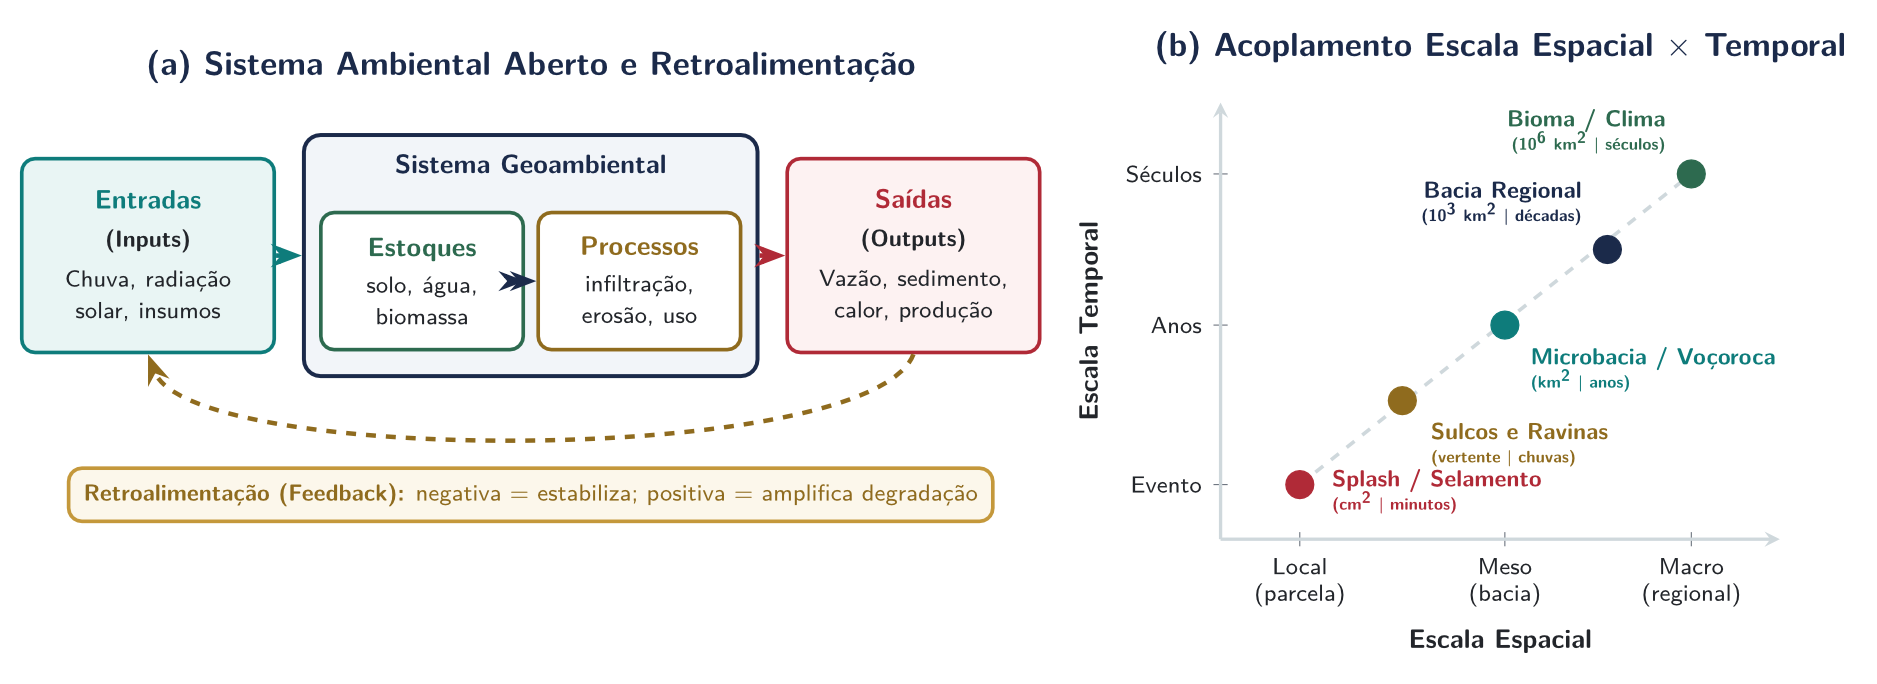
\includegraphics[keepaspectratio]{capitulos/../img/fig04_sistema_aberto_escalas.png}}

}

\caption{\label{fig-sistema_escalas}Representação do sistema ambiental
aberto com entradas, estoques, processos, saídas e retroalimentação
(Painel A) e acoplamento entre escalas espaciais e temporais na dinâmica
geoambiental (Painel B). Fonte, elaboração didática da disciplina CHF662
com base em Drew (1989) e Castro; Lemos (2016).}

\end{figure}%

\subsection{\texorpdfstring{Equilíbrio Dinâmico, Limiares
(\emph{Thresholds}) e
Retroalimentação}{Equilíbrio Dinâmico, Limiares (Thresholds) e Retroalimentação}}\label{equiluxedbrio-dinuxe2mico-limiares-thresholds-e-retroalimentauxe7uxe3o}

\textbf{Equilíbrio dinâmico (\emph{steady state}),} condição em que as
entradas e saídas se compensam em média ao longo do tempo
(\(\Delta S \approx 0\)), mantendo os estoques estáveis apesar da
circulação contínua de água, energia e matéria. Não se trata de
imobilidade, mas de autorregulação ativa. \textbf{Retroalimentação
negativa (\emph{feedback} negativo),} mecanismo \textbf{estabilizador}
que amortece uma perturbação e devolve o sistema ao equilíbrio. Exemplo,
em uma vertente bem vegetada, um aumento moderado de chuva eleva a
umidade do solo \(\to\) estimula o crescimento herbáceo \(\to\) aumenta
a interceptação e a infiltração \(\to\) reduz o escoamento erosivo.

\textbf{Retroalimentação positiva (\emph{feedback} positivo),} mecanismo
\textbf{amplificador} que reforça o desvio inicial, podendo conduzir o
sistema à degradação acelerada. Exemplo clássico de desertificação ou
erosão linear, sobrepastejo reduz cobertura vegetal \(\to\) aumenta
selamento e compactação do solo \(\to\) cai a infiltração e cresce o
escoamento superficial \(\to\) carrega matéria orgânica e sementes
\(\to\) dificulta ainda mais o crescimento vegetal \(\to\) acelera a
abertura de ravinas e voçorocas. \textbf{Limiares (\emph{thresholds}),}
pontos críticos de ruptura a partir dos quais o sistema muda de regime.
Podem ser \textbf{extrínsecos} (disparados por um evento externo, como
uma chuva cuja intensidade ultrapassa a taxa máxima de infiltração do
solo, \(I > f_c\)) ou \textbf{intrínsecos} (resultantes do
enfraquecimento interno gradual do próprio sistema, como o desgaste
progressivo da coesão de um talude até o rompimento repentino).

\subsection{Escalas Espaciais, Escalas Temporais e o Risco da Falácia de
Escala}\label{escalas-espaciais-escalas-temporais-e-o-risco-da-faluxe1cia-de-escala}

Nenhum processo geoambiental ocorre fora de uma escala determinada. Como
mostra o Painel B da Figura~\ref{fig-sistema_escalas}, existe um
\textbf{acoplamento natural entre escala espacial e escala temporal},
processos microscópicos ou pontuais costumam ocorrer em minutos ou
horas, enquanto transformações de bacias regionais e biomas desdobram-se
em décadas, séculos ou milênios.

{\def\LTcaptype{none} % do not increment counter
\begin{longtable}[]{@{}
  >{\raggedright\arraybackslash}p{(\linewidth - 6\tabcolsep) * \real{0.2500}}
  >{\raggedright\arraybackslash}p{(\linewidth - 6\tabcolsep) * \real{0.2500}}
  >{\raggedright\arraybackslash}p{(\linewidth - 6\tabcolsep) * \real{0.2500}}
  >{\raggedright\arraybackslash}p{(\linewidth - 6\tabcolsep) * \real{0.2500}}@{}}
\toprule\noalign{}
\begin{minipage}[b]{\linewidth}\raggedright
\textbf{Escala Espacial}
\end{minipage} & \begin{minipage}[b]{\linewidth}\raggedright
\textbf{Ordem de Área}
\end{minipage} & \begin{minipage}[b]{\linewidth}\raggedright
\textbf{Escala Temporal Típica}
\end{minipage} & \begin{minipage}[b]{\linewidth}\raggedright
\textbf{Processos e Aplicações Dominantes}
\end{minipage} \\
\midrule\noalign{}
\endhead
\bottomrule\noalign{}
\endlastfoot
\textbf{Parcela / Microescala} & \(\text{cm}^2\) a \(10^2\,\text{m}^2\)
& Minutos a horas (evento chuvoso) & Impacto da gota (\emph{splash}),
selamento superficial, infiltração pontual e erosão laminar inicial. \\
\textbf{Vertente / Encosta} & \(10^2\,\text{m}^2\) a \(\text{ha}\) &
Chuvas intensas a ciclos sazonais & Escoamento concentrado, formação de
sulcos e ravinas, deslizamentos de taludes e manejo conservacionista
local. \\
\textbf{Microbacia} & \(1\) a \(50\,\text{km}^2\) & Meses a anos (ciclos
anuais) & Evolução de voçorocas, conectividade vertente-canal, balanço
hídrico local, PRAD e diagnósticos municipais. \\
\textbf{Bacia Regional} & \(10^2\) a \(10^5\,\text{km}^2\) & Anos a
décadas (escala histórica) & Assoreamento de grandes reservatórios,
conflitos pelo uso da água, planos de bacia e ZEE estadual. \\
\textbf{Bioma / Macroescala} & \(> 10^5\,\text{km}^2\) & Décadas a
milênios (tempo geológico/climático) & Dinâmica climática regional,
aridização/desertificação, evolução geomorfológica e grandes políticas
territoriais. \\
\end{longtable}
}

Ignorar o acoplamento entre escalas leva à \textbf{falácia de escala},
um dos erros mais graves na Geografia e na Análise Ambiental. Ela se
manifesta em duas direções opostas,

\textbf{Extrapolação ascendente indevida (micro \(\to\) macro).} Assumir
que uma taxa medida em parcela experimental de \(10\,\text{m}^2\)
multiplica-se linearmente por toda uma bacia de \(1\,000\,\text{ha}\).
Na realidade, grande parte do solo erodido nas encostas fica retida em
sopés côncavos, depressões, barreiras vegetais e planícies aluviais
antes de atingir o rio principal. \textbf{Inferência descendente
indevida (macro \(\to\) micro).} Usar um mapa de escala pequena
(\(1:250\,000\) ou \(1:1\,000\,000\)), elaborado para planejamento
estadual, para localizar uma ravina de \(4\,\text{m}\) de largura ou
projetar uma paliçada de bioengenharia. Em escala cartográfica \(1:D\),
o menor detalhe graficamente distinguível no papel
(\(\approx 0{,}2\,\text{mm} = 0{,}0002\,\text{m}\)) corresponde no
terreno a \(d_{\min} = 0{,}0002 \times D\) metros, em \(1:250\,000\),
qualquer feição menor que \(50\,\text{m}\) simplesmente desaparece do
mapa!

\subsection{Balanço de Massa em Sistema Aberto, Razão de Entrega de
Sedimentos (SDR) e Resolução de
Escala}\label{balanuxe7o-de-massa-em-sistema-aberto-razuxe3o-de-entrega-de-sedimentos-sdr-e-resoluuxe7uxe3o-de-escala}

\textbf{1. Equação geral do balanço em um sistema ambiental aberto,}

\[
\Delta S = E - S_{\text{out}}
\]

Para o \textbf{balanço hídrico} de uma microbacia (em
\(\text{mm/ano}\)),

\[
\Delta S = P - \left(ET + Q_s + Q_b\right)
\]

onde \(P\) é a precipitação (entrada), \(ET\) é a evapotranspiração
real, \(Q_s\) é o escoamento superficial direto e \(Q_b\) é o escoamento
de base/drenagem profunda (saídas). Se \(\Delta S = 0\), há equilíbrio
dinâmico; se \(\Delta S < 0\), ocorre depleção do estoque hídrico do
solo/aquífero; se \(\Delta S > 0\), ocorre recarga.

\textbf{2. Razão de Entrega de Sedimentos (\emph{Sediment Delivery
Ratio}, SDR) e quantificação da falácia de escala,}

\[
\text{SDR} = \frac{Y}{E_b} \qquad \Longleftrightarrow \qquad Y = E_b \times \text{SDR}, \qquad \text{com } 0 < \text{SDR} \le 1
\]

onde \(E_b\) é a erosão bruta nas vertentes
(\(\text{t/(ha}\cdot\text{ano)}\)) e \(Y\) é a produção específica de
sedimentos medida no exutório da bacia
(\(\text{t/(ha}\cdot\text{ano)}\)). Para uma bacia de área \(A\)
(\(\text{ha}\)), sendo \(E_{b,\text{tot}} = E_b \times A\) a erosão
bruta total e \(Y_{\text{tot}} = Y \times A\) o aporte total no exutório
(\(\text{t/ano}\)), a massa total retida internamente nas encostas e
planícies (colúvios e alúvios) é
\(R_{\text{sed}} = (E_b - Y) \times A\). Quando um analista extrapola
dados de parcela para a bacia assumindo implicitamente
\(\text{SDR} = 1\), comete erro relativo de superestimativa igual a,

\[
\text{Erro (\%)} = \frac{E_{b,\text{tot}} - Y_{\text{tot}}}{Y_{\text{tot}}} \times 100\% = \left(\frac{1}{\text{SDR}} - 1\right) \times 100\%.
\]

\textbf{3. Menor feição representável em carta de escala \(1:D\) (erro
gráfico de \(0{,}2\,\text{mm}\)),}

\[
d_{\min}\,(\text{m}) = 0{,}0002 \times D.
\]

\subsection{Dinâmica Geoambiental, Planejamento Ambiental, Planejamento
Territorial e Ordenamento
Territorial}\label{dinuxe2mica-geoambiental-planejamento-ambiental-planejamento-territorial-e-ordenamento-territorial}

Compreender a \textbf{dinâmica geoambiental}, isto é, o comportamento
integrado das paisagens frente às pressões climáticas e socioeconômicas,
é a base técnica indispensável para orientar decisões públicas sobre o
uso do espaço. Contudo, na literatura técnica e em concursos, três
expressões correlatas são frequentemente confundidas,
\textbf{planejamento ambiental}, \textbf{planejamento territorial} e
\textbf{ordenamento territorial} (Arruda, 2013; IBGE, 2018).

{\def\LTcaptype{none} % do not increment counter
\begin{longtable}[]{@{}
  >{\raggedright\arraybackslash}p{(\linewidth - 6\tabcolsep) * \real{0.2500}}
  >{\raggedright\arraybackslash}p{(\linewidth - 6\tabcolsep) * \real{0.2500}}
  >{\raggedright\arraybackslash}p{(\linewidth - 6\tabcolsep) * \real{0.2500}}
  >{\raggedright\arraybackslash}p{(\linewidth - 6\tabcolsep) * \real{0.2500}}@{}}
\toprule\noalign{}
\begin{minipage}[b]{\linewidth}\raggedright
\textbf{Conceito}
\end{minipage} & \begin{minipage}[b]{\linewidth}\raggedright
\textbf{Objeto e foco central}
\end{minipage} & \begin{minipage}[b]{\linewidth}\raggedright
\textbf{Natureza e função}
\end{minipage} & \begin{minipage}[b]{\linewidth}\raggedright
\textbf{Instrumentos típicos}
\end{minipage} \\
\midrule\noalign{}
\endhead
\bottomrule\noalign{}
\endlastfoot
\textbf{Planejamento Ambiental} & Qualidade dos ecossistemas, recursos
naturais, fragilidades, riscos e serviços ecossistêmicos. & Processo
contínuo de diagnóstico, prognóstico e formulação de diretrizes para
conservar, recuperar e compatibilizar atividades humanas à capacidade de
suporte ambiental. & AIA, Planos de Bacia Hidrográfica, Planos de Manejo
de UCs, PRAD, planos municipais de saneamento e conservação. \\
\textbf{Planejamento Territorial} & Organização socioespacial abrangente
(economia, infraestrutura, mobilidade, habitação, redes urbanas e
rurais, incluindo a dimensão ambiental). & Processo estratégico
multissetorial de definição de cenários, prioridades de investimento e
articulação de políticas públicas sobre o território. & Planos Diretores
Municipais, Planos de Desenvolvimento Regional, Planos Plurianuais
territorializados. \\
\textbf{Ordenamento Territorial} & Regulação espacial efetiva da
distribuição das atividades, usos do solo e ocupação humana no
território. & Expressão \textbf{normativa, cartográfica e vinculante} do
Estado para compatibilizar usos produtivos, infraestrutura e proteção
ambiental, reduzindo conflitos socioespaciais. & \textbf{Zoneamento
Ecológico-Econômico (ZEE)}, macrozoneamento do Plano Diretor, zoneamento
costeiro e agrícola. \\
\end{longtable}
}

Em síntese operacional, o \textbf{planejamento ambiental} define os
limites, potenciais e fragilidades dos sistemas naturais; o
\textbf{planejamento territorial} integra esses condicionantes às
demandas econômicas, sociais e de infraestrutura; e o
\textbf{ordenamento territorial} traduz essas diretrizes em normas
espaciais e zoneamentos concretos de regulação do uso da terra.

\subsection{Zoneamento Ecológico-Econômico (ZEE) como Instrumento de
Ordenamento}\label{zoneamento-ecoluxf3gico-econuxf4mico-zee-como-instrumento-de-ordenamento}

Previsto originalmente na Política Nacional do Meio Ambiente (Lei nº
6.938/1981) e regulamentado pelo \textbf{Decreto Federal nº 4.297/2002},
o \textbf{Zoneamento Ecológico-Econômico (ZEE)} é o principal
instrumento técnico-político de organização do território no Brasil. Ele
não é um ``mapa de proibições'', tampouco um documento meramente
cartográfico, trata-se de um processo participativo e multidisciplinar
que cruza a \textbf{potencialidade socioeconômica} com a
\textbf{vulnerabilidade/fragilidade natural} dos sistemas geoambientais
(IBGE, 2018; Arruda, 2013).

A partir desse cruzamento, o território é dividido em \textbf{zonas
homogêneas} com regras específicas de uso, manejo e investimento
público,

\textbf{Zonas de Consolidação Produtiva.} Áreas de alta aptidão e baixa
fragilidade natural, onde o uso agropecuário, industrial ou urbano deve
ser otimizado com boas práticas de conservação de solo e água.
\textbf{Zonas de Uso Restrito ou Manejo Sustentável.} Áreas de
fragilidade média a alta que admitem atividades produtivas de baixo
impacto (extrativismo sustentável, sistemas agroflorestais, ecoturismo,
manejo da Caatinga). \textbf{Zonas de Recuperação Ambiental.} Áreas já
submetidas a processos de degradação (erosão acelerada, desertificação,
matas ciliares suprimidas), prioritárias para PRAD, bioengenharia e
recomposição florestal.

\textbf{Zonas de Proteção e Conservação.} Áreas de altíssima
fragilidade, relevância hídrica ou biodiversidade endêmica (APPs,
nascentes, Unidades de Conservação, corredores ecológicos), voltadas
prioritariamente à preservação.

O ZEE dialoga diretamente com a AIA (Capítulo 5), quando um estado ou
município dispõe de um ZEE atualizado em escala compatível, a etapa de
triagem e a seleção de alternativas locacionais tornam-se muito mais
céleres, transparentes e seguras juridicamente.

\subsection{Balanço ambiental e compatibilidade entre
escalas}\label{balanuxe7o-ambiental-e-compatibilidade-entre-escalas}

Um balanço de água relaciona entradas, saídas e variação do
armazenamento durante um intervalo definido. Precipitação medida em
milímetros representa uma lâmina, enquanto vazão em metros cúbicos por
segundo representa volume por tempo. A comparação exige converter a
lâmina em volume pela área correspondente e integrar a vazão no
intervalo observado.

Em um exemplo didático, uma chuva de 20 mm sobre 2 km² corresponde a
40.000 m³ de água precipitada. A parcela que chega ao exutório depende
da interceptação, da infiltração, da evaporação e do armazenamento. Um
coeficiente de escoamento adotado para o exercício precisa ser
apresentado como hipótese e confrontado com medições quando aplicado a
uma área real.

A integração espacial também exige coerência entre mapas. A ampliação
visual de um mapa regional não acrescenta detalhes sobre uma encosta.
Resolução da imagem, escala de levantamento e unidade mínima de
mapeamento condicionam a leitura. Uma delimitação precisa de APP ou de
feição erosiva depende de informação compatível com essa finalidade.

O diagnóstico deve manter registro de fonte, data, unidade e método de
cada camada. Esse registro permite explicar divergências, selecionar
áreas para verificação em campo e avaliar como as incertezas dos dados
influenciam a proposta de ordenamento.

\section{Etapa 4 - Exemplos
resolvidos}\label{etapa-4---exemplos-resolvidos-5}

\subsection{Exemplo 6.1 - Balanço Hídrico em Sistema Ambiental Aberto no
Semiárido (Nível
Básico)}\label{exemplo-6.1---balanuxe7o-huxeddrico-em-sistema-ambiental-aberto-no-semiuxe1rido-nuxedvel-buxe1sico}

\textbf{Situação analisada.} Uma microbacia experimental inserida no
domínio da Caatinga foi monitorada durante um ano hidrológico completo.
Deseja-se avaliar se o sistema hídrico local operou em equilíbrio
dinâmico, recarga ou depleção de estoque.

\textbf{Dados disponíveis.} Entrada anual de precipitação
\(P = 680\,\text{mm/ano}\). Saídas anuais medidas, evapotranspiração
real \(ET = 545\,\text{mm/ano}\); escoamento superficial direto
\(Q_s = 115\,\text{mm/ano}\); escoamento de base / drenagem profunda
\(Q_b = 35\,\text{mm/ano}\).

\textbf{Problema a resolver.} Calcular o total de saídas
(\(S_{\text{out}}\)), a variação do estoque hídrico interno
(\(\Delta S\)) e interpretar o estado funcional do sistema nesse ano
hidrológico.

\textbf{Fundamento da análise.} Aplicação da equação de conservação de
massa em sistema ambiental aberto, \(\Delta S = P - (ET + Q_s + Q_b)\).

\textbf{Desenvolvimento.}

\textbf{Soma das saídas do sistema (\(S_{\text{out}}\)),}

\[
S_{\text{out}} = ET + Q_s + Q_b = 545 + 115 + 35 = 695\,\text{mm/ano}.
\]

. \textbf{Variação do estoque hídrico (\(\Delta S\)),}

\[
\Delta S = P - S_{\text{out}} = 680 - 695 = -15\,\text{mm/ano}.
\]

. \textbf{Interpretação física.} O sinal negativo
(\(\Delta S = -15\,\text{mm/ano}\)) indica que as saídas superaram as
entradas em \(15\,\text{mm}\); logo, o sistema consumiu parte da água
armazenada previamente no solo e nos reservatórios subterrâneos rasos
(depleção líquida de estoque).

\textbf{Interpretação do resultado.} Total de saídas
\(S_{\text{out}} = 695\,\text{mm/ano}\) e variação do estoque
\(\Delta S = -15\,\text{mm/ano}\), caracterizando depleção moderada do
estoque hídrico interno nesse ano.

\textbf{Condições de validade.} O valor é fisicamente coerente para o
Semiárido baiano, a evapotranspiração consome a maior parcela da chuva
(\(545/680 \approx 80{,}15\%\)), e déficits interanuais moderados de
estoque são esperados em anos de precipitação ligeiramente abaixo da
média, sendo compensados nos anos mais chuvosos se a cobertura vegetal
preservar a infiltração.

\subsection{Exemplo 6.2 - Quantificando a Falácia de Escala pela Razão
de Entrega de Sedimentos, SDR (Nível
Básico-Intermediário)}\label{06-analise-ambiental-integrada-exemplo-6.2.-quantificando-a-faluxe1cia-de-escala-pela-razuxe3o-de-entrega-de-sedimentos-sdr-nuxedvel-buxe1sicointermediuxe1rio}

\textbf{Situação analisada.} Em uma parcela experimental de
\(20\,\text{m}^2\) de solo exposto em uma microbacia do Piemonte da
Diamantina, mediu-se uma taxa de erosão bruta de
\(E_b = 24{,}0\,\text{t/(ha}\cdot\text{ano)}\). Para estimar o
assoreamento de um açude no exutório da bacia (área total
\(A = 1\,500\,\text{ha}\)), um técnico multiplicou diretamente a taxa da
parcela pela área da bacia. Entretanto, o monitoramento
hidrossedimentológico no exutório registrou uma chegada efetiva de
\(Y_{\text{tot}} = 9\,720\,\text{t/ano}\).

\textbf{Dados disponíveis.}
\(E_b = 24{,}0\,\text{t/(ha}\cdot\text{ano)}\); área da bacia
\(A = 1\,500\,\text{ha}\); produção total medida no exutório
\(Y_{\text{tot}} = 9\,720\,\text{t/ano}\).

\textbf{Problema a resolver.} Calcular, (a) a erosão bruta total
estimada pela extrapolação linear do técnico; (b) a produção específica
real \(Y\); (c) a Razão de Entrega de Sedimentos (SDR); (d) a massa
anual de sedimentos retida nas vertentes e planícies; e (e) o erro
percentual causado pela falácia de escala.

\textbf{Fundamento da análise.} Aplicação das relações de escala
hidrossedimentológica, \(E_{b,\text{tot}} = E_b \cdot A\),
\(Y = Y_{\text{tot}}/A\), \(\text{SDR} = Y / E_b\),
\(R_{\text{sed}} = E_{b,\text{tot}} - Y_{\text{tot}}\) e
\(\text{Erro (\%)} = (E_{b,\text{tot}} - Y_{\text{tot}})/Y_{\text{tot}} \times 100\%\).

\textbf{Desenvolvimento.}

\textbf{Extrapolação linear do técnico (erosão bruta total),}

\[
E_{b,\text{tot}} = 24{,}0\,\text{t/(ha}\cdot\text{ano)} \times 1\,500\,\text{ha} = 36\,000\,\text{t/ano}.
\]

. \textbf{Produção específica real de sedimentos no exutório (\(Y\)),}

\[
Y = \frac{9\,720\,\text{t/ano}}{1\,500\,\text{ha}} = 6{,}48\,\text{t/(ha}\cdot\text{ano)}.
\]

. \textbf{Razão de Entrega de Sedimentos (SDR),}

\[
\text{SDR} = \frac{Y}{E_b} = \frac{6{,}48}{24{,}0} = 0{,}27 \quad (\text{ou } 27\%).
\]

. \textbf{Massa de sedimentos retida internamente na bacia,}

\[
R_{\text{sed}} = 36\,000 - 9\,720 = 26\,280\,\text{t/ano} \quad (73\% \text{ do solo mobilizado}).
\]

. \textbf{Erro percentual de superestimativa (falácia de escala),}

\[
\text{Erro (\%)} = \frac{36\,000 - 9\,720}{9\,720} \times 100\% = \frac{26\,280}{9\,720} \times 100\% \approx 270{,}37\%.
\]

.

\textbf{Interpretação do resultado.}
\(E_{b,\text{tot}} = 36\,000\,\text{t/ano}\);
\(Y = 6{,}48\,\text{t/(ha}\cdot\text{ano)}\); \(\text{SDR} = 0{,}27\);
sedimentos retidos \(= 26\,280\,\text{t/ano}\); erro de superestimativa
\(= 270{,}37\%\).

\textbf{Condições de validade.} Confere-se a fórmula alternativa do
erro,
\((1/\text{SDR} - 1)\times 100\% = (1/0{,}27 - 1)\times 100\% = (3{,}7037 - 1)\times 100\% = 270{,}37\%\).
Ambientalmente, esse resultado demonstra a essência da \textbf{falácia
de escala}, taxas medidas em parcela de \(20\,\text{m}^2\) não
consideram a rede de deposição em sopés, depressões e matas ciliares que
retém \(73\%\) dos sedimentos ao longo de uma bacia de
\(1\,500\,\text{ha}\).

\subsection{Exemplo 6.3 - Limiar de Infiltração e Retroalimentação
Positiva versus Negativa (Nível
Intermediário)}\label{exemplo-6.3---limiar-de-infiltrauxe7uxe3o-e-retroalimentauxe7uxe3o-positiva-versus-negativa-nuxedvel-intermediuxe1rio}

\textbf{Situação analisada.} Duas vertentes vizinhas com mesma litologia
e declividade no Semiárido baiano recebem a mesma chuva convectiva
intensa de \(I = 65{,}0\,\text{mm/h}\) durante \(1\) hora. A
\textbf{Vertente 1} possui cobertura de Caatinga conservada com
serrapilheira e capacidade de infiltração estável
\(f_{c1} = 78{,}0\,\text{mm/h}\). A \textbf{Vertente 2} foi submetida a
sobrepastejo contínuo, apresentando solo compactado com capacidade de
infiltração reduzida para \(f_{c2} = 22{,}0\,\text{mm/h}\).

\textbf{Dados disponíveis.} Intensidade da chuva
\(I = 65{,}0\,\text{mm/h}\); limiar de infiltração da Vertente 1,
\(f_{c1} = 78{,}0\,\text{mm/h}\); limiar de infiltração da Vertente 2,
\(f_{c2} = 22{,}0\,\text{mm/h}\).

\textbf{Problema a resolver.} Calcular o excesso de precipitação
transformado em escoamento superficial (\(R = \max(0, I - f_c)\)) e o
percentual da chuva que escoa superficialmente em cada vertente,
identificando em qual delas o limiar extrínseco foi rompido e qual tipo
de retroalimentação predomina.

\textbf{Fundamento da análise.} Comparação direta entre a entrada
externa (\(I\)) e o limiar interno de infiltração (\(f_c\)), seguida da
análise sistêmica dos circuitos de retroalimentação.

\textbf{Desenvolvimento.}

\textbf{Vertente 1 (Caatinga conservada),} Como
\(I = 65{,}0\,\text{mm/h} < f_{c1} = 78{,}0\,\text{mm/h}\), o limiar de
infiltração \textbf{não é ultrapassado},

\[
R_1 = \max(0,\; 65{,}0 - 78{,}0) = 0{,}0\,\text{mm/h} \quad (0\% \text{ de escoamento hortoniano}).
\]

Toda a lâmina de \(65{,}0\,\text{mm}\) infiltra-se, recarregando a
umidade do solo, sustentando a vegetação e mantendo a estrutura porosa
(\textbf{retroalimentação negativa}, estabilizadora). \textbf{Vertente 2
(Pastagem compactada),} Como
\(I = 65{,}0\,\text{mm/h} > f_{c2} = 22{,}0\,\text{mm/h}\), o limiar de
infiltração é \textbf{rompido},

\[
R_2 = 65{,}0 - 22{,}0 = 43{,}0\,\text{mm/h}.
\]

. \textbf{Percentual da chuva convertido em escoamento superficial na
Vertente 2,}

\[
\frac{R_2}{I} \times 100\% = \frac{43{,}0}{65{,}0} \times 100\% \approx 66{,}15\%.
\]

Mais de dois terços da chuva escoam velozmente pela superfície,
removendo solo fértil, sementes e nutrientes, o que dificulta a
regeneração vegetal e reduz ainda mais \(f_c\) nas chuvas seguintes
(\textbf{retroalimentação positiva}, amplificadora da degradação).

\textbf{Interpretação do resultado.} Vertente 1,
\(R_1 = 0{,}0\,\text{mm/h}\) (\(0\%\), abaixo do limiar,
retroalimentação negativa). Vertente 2, \(R_2 = 43{,}0\,\text{mm/h}\)
(\(66{,}15\%\) da chuva vira enxurrada, limiar rompido, retroalimentação
positiva degradativa).

\textbf{Condições de validade.} O contraste entre \(0\,\text{mm/h}\) e
\(43{,}0\,\text{mm/h}\) sob exatamente a mesma chuva demonstra que a
degradação no Semiárido não decorre apenas da ``força da natureza'', mas
da interação entre o evento climático (meio físico) e o manejo do
solo/vegetação (meios biótico e antrópico).

\subsection{Exemplo 6.4 - Escolha de Escala Cartográfica e Erro Gráfico
Mínimo em Diagnósticos (Nível
Intermediário-Avançado)}\label{06-analise-ambiental-integrada-exemplo-6.4.-escolha-de-escala-cartogruxe1fica-e-erro-gruxe1fico-muxednimo-em-diagnuxf3sticos-nuxedvel-intermediuxe1rioavanuxe7ado}

\textbf{Situação analisada.} Uma equipe de Geografia precisa mapear
ravinas com largura média de \(4{,}0\,\text{m}\) e faixas de mata ciliar
de \(15{,}0\,\text{m}\) em uma microbacia de \(850\,\text{ha}\)
(\(8{,}5\,\text{km}^2\)) próxima a Feira de Santana. A prefeitura dispõe
de três bases cartográficas, uma carta regional do ZEE (\(1:250\,000\)),
uma carta topográfica sistemática (\(1:50\,000\)) e um ortomosaico
detalhado (\(1:10\,000\)).

\textbf{Dados disponíveis.} Erro gráfico mínimo no papel
\(= 0{,}2\,\text{mm} = 0{,}0002\,\text{m}\); escalas disponíveis,
\(D_1 = 250\,000\), \(D_2 = 50\,000\) e \(D_3 = 10\,000\); alvos de
mapeamento, ravinas (\(4{,}0\,\text{m}\)) e mata ciliar
(\(15{,}0\,\text{m}\)).

\textbf{Problema a resolver.} Calcular a menor feição representável no
terreno (\(d_{\min}\)) em cada escala e determinar qual base é
tecnicamente adequada para mapear os dois alvos sem incorrer em falácia
de escala.

\textbf{Fundamento da análise.} Aplicação da relação de resolução
gráfica cartográfica \(d_{\min} = 0{,}0002 \times D\) e comparação
direta com a largura real das feições-alvo.

\textbf{Desenvolvimento.}

\textbf{Carta regional (\(1:250\,000\)),}

\[
d_{\min,1} = 0{,}0002 \times 250\,000 = 50{,}0\,\text{m}.
\]

Nem a mata ciliar (\(15{,}0\,\text{m} < 50{,}0\,\text{m}\)) nem as
ravinas (\(4{,}0\,\text{m} < 50{,}0\,\text{m}\)) podem ser representadas
com fidelidade geométrica. \textbf{Carta topográfica municipal
(\(1:50\,000\)),}

\[
d_{\min,2} = 0{,}0002 \times 50\,000 = 10{,}0\,\text{m}.
\]

A mata ciliar (\(15{,}0\,\text{m} > 10{,}0\,\text{m}\)) já é
representável, porém as ravinas (\(4{,}0\,\text{m} < 10{,}0\,\text{m}\))
permanecem abaixo do limite gráfico. \textbf{Base detalhada
(\(1:10\,000\)),}

\[
d_{\min,3} = 0{,}0002 \times 10\,000 = 2{,}0\,\text{m}.
\]

Tanto a mata ciliar (\(15{,}0\,\text{m} > 2{,}0\,\text{m}\)) quanto as
ravinas (\(4{,}0\,\text{m} > 2{,}0\,\text{m}\)) são representáveis em
escala real.

\textbf{Interpretação do resultado.} As menores feições representáveis
são \(50{,}0\,\text{m}\) (\(1:250\,000\)), \(10{,}0\,\text{m}\)
(\(1:50\,000\)) e \(2{,}0\,\text{m}\) (\(1:10\,000\)). Somente a escala
\(1:10\,000\) (ou maior detalhe, como \(1:5\,000\) obtida por
drone/VANT) permite mapear simultaneamente as ravinas de
\(4{,}0\,\text{m}\) e a mata ciliar de \(15{,}0\,\text{m}\).

\textbf{Condições de validade.} Concluir que ``não existem ravinas na
microbacia'' após inspecionar uma carta \(1:250\,000\) seria um exemplo
clássico de falácia de escala descendente, a ausência no mapa reflete a
limitação da escala escolhida, não a inexistência do processo erosivo em
campo.

\subsection{Exemplo 6.5 - Zoneamento Ecológico-Econômico (ZEE) e
Articulação com o Ordenamento Territorial (Nível
Avançado)}\label{exemplo-6.5---zoneamento-ecoluxf3gico-econuxf4mico-zee-e-articulauxe7uxe3o-com-o-ordenamento-territorial-nuxedvel-avanuxe7ado}

\textbf{Situação analisada.} Após integrar levantamentos de solos,
declividade, remanescentes de Caatinga, recursos hídricos e uso
agropecuário, um município baiano de \(1\,200\,\text{km}^2\) elaborou
sua proposta de Zoneamento Ecológico-Econômico (ZEE), distribuindo o
território em quatro zonas.

\textbf{Dados disponíveis.} Área total do município
\(= 1\,200\,\text{km}^2\),

\(Z_1\), Zona de Consolidação Produtiva, \(420\,\text{km}^2\);. \(Z_2\),
Zona de Expansão com Manejo Sustentável, \(330\,\text{km}^2\);. \(Z_3\),
Zona de Recuperação Ambiental (áreas degradadas/erosão),
\(210\,\text{km}^2\);. \(Z_4\), Zona de Proteção e Conservação
(nascentes, serras e UCs), \(240\,\text{km}^2\).

\textbf{Problema a resolver.} Verificar o fechamento territorial das
áreas, calcular o percentual de cada zona, determinar o percentual
conjunto destinado à conservação e recuperação (\(Z_3 + Z_4\)) e
distinguir o papel do planejamento ambiental, do planejamento
territorial e do ordenamento territorial nesse caso.

\textbf{Fundamento da análise.} Cálculo de participação percentual
(\(A_k / A_{\text{total}} \times 100\%\)) e classificação funcional
conforme Arruda (2013) e IBGE (2018).

\textbf{Desenvolvimento.}

\textbf{Verificação da soma das áreas,}
\(420 + 330 + 210 + 240 = 1\,200\,\text{km}^2\) (\(100{,}0\%\),
fechamento exato). \textbf{Percentual de cada zona,}

\[
\begin{aligned}
\%Z_1 &= \frac{420}{1\,200} \times 100\% = 35{,}0\%, & \%Z_2 &= \frac{330}{1\,200} \times 100\% = 27{,}5\%, \\
\%Z_3 &= \frac{210}{1\,200} \times 100\% = 17{,}5\%, & \%Z_4 &= \frac{240}{1\,200} \times 100\% = 20{,}0\%.
\end{aligned}
\]

. \textbf{Soma das zonas de proteção e recuperação (\(Z_3 + Z_4\)),}

\[
A_{3+4} = 210 + 240 = 450\,\text{km}^2 \implies \frac{450}{1\,200} \times 100\% = 37{,}5\% \quad (\text{ou } 17{,}5\% + 20{,}0\% = 37{,}5\%).
\]

. \textbf{Articulação conceitual.} O \textbf{planejamento ambiental}
forneceu o diagnóstico integrado de solos, nascentes, fragilidades e
áreas degradadas (\(Z_3\) e \(Z_4\)); o \textbf{planejamento
territorial} compatibilizou essas informações com as metas de produção
agropecuária, estradas e abastecimento urbano (\(Z_1\) e \(Z_2\)); o
\textbf{ordenamento territorial} normatizou o mapa final do ZEE em
lei/decreto, vinculando licenciamento ambiental, crédito rural e
investimentos públicos às regras de cada zona.

\textbf{Interpretação do resultado.} \(Z_1 = 35{,}0\%\),
\(Z_2 = 27{,}5\%\), \(Z_3 = 17{,}5\%\) e \(Z_4 = 20{,}0\%\); conservação
e recuperação somam \(450\,\text{km}^2\) (\(37{,}5\%\) do município). O
ZEE materializa o ordenamento territorial apoiado pelos planejamentos
ambiental e territorial.

\textbf{Condições de validade.} A soma dos percentuais fecha em
\(35{,}0 + 27{,}5 + 17{,}5 + 20{,}0 = 100{,}0\%\). Territorialmente,
reservar \(37{,}5\%\) para proteção e recuperação enquanto se direcionam
\(62{,}5\%\) para produção consolidada e manejo sustentável mostra que o
ZEE não paralisa o desenvolvimento econômico, mas o redireciona para
áreas com capacidade de suporte adequada.

\section{Etapa 5 - Erros de
interpretação}\label{etapa-5---erros-de-interpretauxe7uxe3o-5}

\subsection{Erro 1, Confundir retroalimentação positiva com algo ``bom''
ou
desejável}\label{erro-1-confundir-retroalimentauxe7uxe3o-positiva-com-algo-bom-ou-desejuxe1vel}

\textbf{Equívoco frequente.} Interpretar ``retroalimentação positiva''
como um processo ambientalmente benéfico e ``retroalimentação negativa''
como algo prejudicial.

\textbf{Por que está incorreto.} Na Teoria dos Sistemas, os adjetivos
\emph{positivo} e \emph{negativo} têm sentido matemático/cibernético,
não moral. \textbf{Negativa} significa que o retorno \emph{opõe-se} ao
desvio inicial e estabiliza o sistema; \textbf{positiva} significa que o
retorno \emph{soma-se} ao desvio inicial e o amplifica, constituindo o
motor típico de voçorocamentos, desertificação e colapsos ecológicos.

\textbf{Como evitar.} Associe sempre \textbf{negativa = freio
estabilizador} e \textbf{positiva = acelerador/bola de neve}.

\subsection{Erro 2, Praticar a falácia de escala extrapolando dados de
parcela diretamente para a
bacia}\label{erro-2-praticar-a-faluxe1cia-de-escala-extrapolando-dados-de-parcela-diretamente-para-a-bacia}

\textbf{Equívoco frequente.} Multiplicar a perda de solo medida em
parcela de \(10\,\text{m}^2\) pela área inteira de uma bacia de
\(5\,000\,\text{ha}\) e afirmar que toda aquela massa chegará ao rio
principal.

\textbf{Por que está incorreto.} Ignora os estoques intermediários e a
deposição ao longo das encostas e planícies (Razão de Entrega de
Sedimentos \(\text{SDR} < 1\)). Do mesmo modo, utilizar cartas regionais
(\(1:250\,000\)) para diagnosticar feições de poucos metros omite
processos críticos locais.

\textbf{Como evitar.} Explicite sempre a escala espacial e temporal da
medição e verifique se o modelo ou a carta escolhida possui resolução
compatível com o fenômeno analisado.

\subsection{Erro 3, Reduzir a Análise Ambiental Integrada à soma de
relatórios setoriais
desconexos}\label{erro-3-reduzir-a-anuxe1lise-ambiental-integrada-uxe0-soma-de-relatuxf3rios-setoriais-desconexos}

\textbf{Equívoco frequente.} Entregar um trabalho com uma seção de
geologia, uma de vegetação e uma de população que nunca se referenciam
entre si.

\textbf{Por que está incorreto.} Sem explicitar como a declividade e o
solo respondem à retirada da vegetação e como isso repercute no uso da
terra e na oferta hídrica, não há análise integrada, apenas um
inventário descritivo fragmentado.

\textbf{Como evitar.} Ao redigir qualquer diagnóstico, use verbos de
processo e encadeamento (infiltra, concentra, carreia, protege,
amplifica, restringe) conectando explicitamente os meios físico, biótico
e antrópico.

\subsection{Erro 4, Tratar planejamento ambiental, planejamento
territorial e ordenamento territorial como
sinônimos}\label{erro-4-tratar-planejamento-ambiental-planejamento-territorial-e-ordenamento-territorial-como-sinuxf4nimos}

\textbf{Equívoco frequente.} Usar os três termos de maneira
intercambiável em provas ou confundir ZEE com simples criação de
Unidades de Conservação.

\textbf{Por que está incorreto.} Embora articulados, possuem recortes
distintos, o planejamento ambiental foca processos e limites ecológicos;
o planejamento territorial integra todas as dimensões socioespaciais e
de infraestrutura; o ordenamento territorial corresponde à regulação
espacial normativa do uso da terra (tendo no ZEE um instrumento que
abrange tanto zonas produtivas quanto zonas de recuperação e
conservação).

\textbf{Como evitar.} Memorize a tríade funcional, \emph{limites
ambientais} (planejamento ambiental) \(\to\) \emph{estratégia
multissetorial} (planejamento territorial) \(\to\) \emph{regulação
espacial normativa} (ordenamento territorial / ZEE).

\section{Etapa 6 - Exercícios de
fixação}\label{etapa-6---exercuxedcios-de-fixauxe7uxe3o-5}

\subsubsection{Nível 1, Básico (Sistemas Abertos, Escalas e
Ordenamento)}\label{nuxedvel-1-buxe1sico-sistemas-abertos-escalas-e-ordenamento}

\begin{enumerate}
\def\labelenumi{\arabic{enumi}.}
\item
  Explique por que uma bacia hidrográfica é classificada como um
  \textbf{sistema ambiental aberto}, exemplificando duas entradas, dois
  estoques internos, dois processos e duas saídas.
\item
  Diferencie \textbf{retroalimentação negativa} e
  \textbf{retroalimentação positiva} em sistemas ambientais,
  apresentando um exemplo concreto de cada mecanismo na dinâmica erosiva
  de uma encosta.
\item
  Um açude no Semiárido baiano recebeu em um ano
  \(E = 12\,500\,\text{t/ano}\) de sedimentos transportados pelos
  riachos afluentes e exportou pelo vertedouro
  \(S_{\text{out}} = 3\,200\,\text{t/ano}\). Calcule a variação do
  estoque de sedimentos retidos no reservatório (\(\Delta S\)) e a
  eficiência percentual de retenção de sedimentos do açude.
\item
  O que é \textbf{falácia de escala} na Análise Ambiental? Dê um exemplo
  de erro cometido ao passar da microescala para a macroescala e outro
  ao passar da macroescala para a microescala.
\item
  Estabeleça a diferença conceitual entre \textbf{planejamento
  ambiental}, \textbf{planejamento territorial} e \textbf{ordenamento
  territorial}, situando o papel do Zoneamento Ecológico-Econômico
  (ZEE).
\end{enumerate}

\subsubsection{Nível 2, Intermediário (Cálculos Sistêmicos, Escalas e
ZEE)}\label{nuxedvel-2-intermediuxe1rio-cuxe1lculos-sistuxeamicos-escalas-e-zee}

\begin{enumerate}
\def\labelenumi{\arabic{enumi}.}
\setcounter{enumi}{5}
\item
  Em uma microbacia de \(800\,\text{ha}\), a erosão bruta média das
  vertentes estimada por parcelas é
  \(E_b = 18{,}0\,\text{t/(ha}\cdot\text{ano)}\). Sabe-se que a Razão de
  Entrega de Sedimentos da microbacia é \(\text{SDR} = 0{,}32\).
  Calcule, (a) a erosão bruta total (\(E_{b,\text{tot}}\)); (b) a
  produção específica (\(Y\)) e total (\(Y_{\text{tot}}\)) de sedimentos
  no exutório; (c) a massa anual retida nas vertentes e planícies; e (d)
  o erro percentual de superestimativa que ocorreria caso um analista
  assumisse \(\text{SDR} = 1\).
\item
  Uma mesma microbacia recebeu precipitação anual de
  \(P = 750\,\text{mm/ano}\) em dois cenários de cobertura do solo,

  \begin{itemize}
  \item
    \textbf{Cenário 1 (Vegetação nativa conservada),}
    \(ET = 590\,\text{mm}\), \(Q_s = 90\,\text{mm}\),
    \(Q_b = 70\,\text{mm}\).
  \item
    \textbf{Cenário 2 (Após desmatamento e compactação),}
    \(ET = 430\,\text{mm}\), \(Q_s = 340\,\text{mm}\),
    \(Q_b = 25\,\text{mm}\).
  \end{itemize}

  Calcule \(\Delta S\) em ambos os cenários, determine que percentual da
  chuva virou escoamento superficial (\(Q_s/P\)) no Cenário 2 e
  interprete as consequências para a vazão na estiagem (\(Q_b\)) e para
  a erosão.
\item
  Utilizando o erro gráfico mínimo de \(0{,}2\,\text{mm}\) no papel
  (\(d_{\min} = 0{,}0002 \times D\)), calcule a menor feição
  representável no terreno para as escalas \(1:100\,000\), \(1:25\,000\)
  e \(1:5\,000\). Em seguida, informe quais dessas escalas conseguem
  representar, (a) uma faixa de mata ciliar de \(15{,}0\,\text{m}\) de
  largura; (b) uma ravina incipiente de \(1{,}5\,\text{m}\) de largura.
\item
  Explique a diferença entre \textbf{limiar extrínseco} e \textbf{limiar
  intrínseco} na dinâmica geoambiental, ilustrando cada tipo com um
  processo real de instabilidade de encostas ou erosão no Brasil.
\item
  O ZEE de uma sub-bacia hidrográfica de \(2\,500\,\text{km}^2\) definiu
  a seguinte repartição percentual, \(40\%\) de Zona de Consolidação
  Produtiva, \(26\%\) de Zona de Manejo Sustentável, \(16\%\) de Zona de
  Recuperação Ambiental e \(18\%\) de Zona de Proteção e Conservação.
  Calcule a área em \(\text{km}^2\) de cada zona e verifique se o plano
  atende a uma diretriz estadual que exige no mínimo \(30\%\) do
  território sob conservação ou recuperação.
\end{enumerate}

\subsubsection{Nível 3, Questões Objetivas de Fixação
(A-E)}\label{06-analise-ambiental-integrada-nuxedvel-3-questuxf5es-objetivas-de-fixauxe7uxe3o-ae}

\begin{enumerate}
\def\labelenumi{\arabic{enumi}.}
\setcounter{enumi}{10}
\item
  \textbf{{[}Autoral, CHF662{]}} Em uma vertente degradada do Semiárido,
  a remoção da Caatinga expõe o solo ao impacto das gotas de chuva,
  gerando crosta superficial, redução da infiltração, aumento da
  enxurrada e carreamento de matéria orgânica, o que impede a germinação
  de novas plantas e intensifica ainda mais a erosão. Na teoria dos
  sistemas ambientais, esse encadeamento caracteriza,

  \begin{enumerate}
  \def\labelenumii{(\Alph{enumii})}
  \item
    Sistema fechado em equilíbrio termodinâmico estático.
  \item
    Retroalimentação negativa de autorregulação ecológica.
  \item
    Retroalimentação positiva amplificadora da degradação.
  \item
    Neutralidade escalar sem rompimento de limiar.
  \item
    Ciclo biogeoquímico conservativo com ganho de estoque edáfico.
  \end{enumerate}
\item
  \textbf{{[}Autoral, CHF662{]}} Sobre o acoplamento entre escalas
  espaciais e temporais na Análise Ambiental Integrada, assinale a
  alternativa correta,

  \begin{enumerate}
  \def\labelenumii{(\Alph{enumii})}
  \item
    Processos como o impacto da gota de chuva (\emph{splash}) e o
    selamento superficial atuam na macroescala continental ao longo de
    milênios.
  \item
    A dinâmica de uma microbacia ou a evolução de voçorocas
    manifestam-se tipicamente na escala local a mesoescala, ao longo de
    meses e anos.
  \item
    A escala temporal é independente da escala espacial, podendo
    qualquer processo ser monitorado em um único dia de campo.
  \item
    Cartas na escala \(1:1\,000\,000\) são ideais para medir a largura
    de sulcos erosivos em pequenas propriedades rurais.
  \item
    O estudo de biomas prescinde de séries históricas pluridecadais por
    depender apenas de eventos horários isolados.
  \end{enumerate}
\item
  \textbf{{[}Autoral, CHF662{]}} Qual alternativa distingue corretamente
  \textbf{ordenamento territorial} de \textbf{planejamento ambiental}?

  \begin{enumerate}
  \def\labelenumii{(\Alph{enumii})}
  \item
    O ordenamento territorial restringe-se ao monitoramento químico da
    água, enquanto o planejamento ambiental define a malha rodoviária.
  \item
    O planejamento ambiental diagnostica fragilidades, riscos e
    capacidades de suporte dos ecossistemas, ao passo que o ordenamento
    territorial traduz diretrizes socioespaciais e ambientais em
    regulação normativa e espacial dos usos da terra (como o ZEE).
  \item
    O ordenamento territorial é facultativo e exclusivamente acadêmico,
    enquanto o planejamento ambiental não utiliza mapas.
  \item
    O planejamento ambiental proíbe qualquer atividade produtiva,
    enquanto o ordenamento territorial dispensa critérios ecológicos.
  \item
    Ambos são sinônimos perfeitos de licenciamento ambiental de obras
    pontuais.
  \end{enumerate}
\item
  \textbf{{[}Autoral, CHF662{]}} Em uma bacia de \(600\,\text{ha}\),
  medições em parcela indicaram erosão bruta de
  \(15{,}0\,\text{t/(ha}\cdot\text{ano)}\). Sabendo que a Razão de
  Entrega de Sedimentos da bacia é \(\text{SDR} = 0{,}40\), a produção
  anual de sedimentos que efetivamente chega ao exutório e a massa
  retida internamente nas vertentes e planícies são, respectivamente,

  \begin{enumerate}
  \def\labelenumii{(\Alph{enumii})}
  \item
    \(9\,000\,\text{t/ano}\) e \(0\,\text{t/ano}\).
  \item
    \(5\,400\,\text{t/ano}\) e \(3\,600\,\text{t/ano}\).
  \item
    \(3\,600\,\text{t/ano}\) e \(5\,400\,\text{t/ano}\).
  \item
    \(2\,400\,\text{t/ano}\) e \(6\,600\,\text{t/ano}\).
  \item
    \(6\,000\,\text{t/ano}\) e \(3\,000\,\text{t/ano}\).
  \end{enumerate}
\item
  \textbf{{[}Autoral, CHF662{]}} De acordo com o Decreto Federal nº
  4.297/2002 e os fundamentos do IBGE (2018), o \textbf{Zoneamento
  Ecológico-Econômico (ZEE)} caracteriza-se por,

  \begin{enumerate}
  \def\labelenumii{(\Alph{enumii})}
  \item
    Ser um mapa exclusivamente voltado à demarcação de parques
    nacionais, excluindo áreas agrícolas e urbanas.
  \item
    Integrar potencialidades socioeconômicas e
    vulnerabilidades/fragilidades geoambientais para dividir o
    território em zonas com diretrizes específicas de uso, manejo,
    recuperação e proteção.
  \item
    Substituir a obrigatoriedade do Estudo de Impacto Ambiental (EIA)
    para grandes hidrelétricas e minerações.
  \item
    Operar apenas na escala de parcela experimental (\(1:500\)), sendo
    inviável em estados ou bacias regionais.
  \item
    Utilizar apenas variáveis climáticas, dispensando informações de
    solos, relevo e estrutura social.
  \end{enumerate}
\end{enumerate}

\section{Etapa 7 - Questões de
aplicação}\label{etapa-7---questuxf5es-de-aplicauxe7uxe3o-5}

\begin{enumerate}
\def\labelenumi{\arabic{enumi}.}
\setcounter{enumi}{15}
\item
  \textbf{{[}Autoral, Estilo ENADE / Geografia{]}} A abordagem sistêmica
  aplicada à Análise Ambiental Integrada (Drew, 1989; Castro; Lemos,
  2016) compreende a paisagem como resultado de interações dinâmicas
  entre fluxos de matéria, energia e decisões humanas. Avalie as
  asserções a seguir e a relação proposta entre elas,

  \begin{quote}
  \textbf{I.} A extrapolação linear de taxas de perda de solo obtidas em
  pequenas parcelas experimentais para grandes bacias hidrográficas
  costuma superestimar significativamente o aporte real de sedimentos no
  exutório.

  \textbf{PORQUE}

  \textbf{II.} Ao mudar da escala de parcela para a escala de bacia,
  emergem processos intermediários de desconectividade e deposição em
  sopés, depressões, barreiras vegetais e planícies aluviais, fazendo
  com que a Razão de Entrega de Sedimentos (SDR) seja inferior a \(1\).
  \end{quote}

  A respeito dessas asserções, assinale a opção correta,

  \begin{enumerate}
  \def\labelenumii{(\Alph{enumii})}
  \item
    As asserções I e II são proposições verdadeiras, e a II é uma
    justificativa correta da I.
  \item
    As asserções I e II são proposições verdadeiras, mas a II não é uma
    justificativa correta da I.
  \item
    A asserção I é uma proposição verdadeira, e a II é uma proposição
    falsa.
  \item
    A asserção I é uma proposição falsa, e a II é uma proposição
    verdadeira.
  \item
    As asserções I e II são proposições falsas.
  \end{enumerate}
\item
  \textbf{{[}Autoral, Estilo Concurso Geógrafo / Planejamento
  Territorial{]}} Considere o balanço de um sistema ambiental aberto
  sujeito a intervenções humanas. Analise as proposições abaixo,

  \begin{enumerate}
  \def\labelenumii{\Roman{enumii}.}
  \item
    Quando a entrada de energia ou matéria ultrapassa um limiar
    (\emph{threshold}) crítico do sistema, como uma chuva cuja
    intensidade excede a capacidade de infiltração de um solo
    compactado, ocorre mudança brusca no comportamento hidrológico da
    vertente.
  \item
    No equilíbrio dinâmico (\emph{steady state}), os fluxos de entrada e
    saída cessam completamente, impedindo qualquer troca com o entorno.
  \item
    A substituição de vegetação nativa por superfícies impermeabilizadas
    tende a elevar o escoamento superficial direto (\(Q_s\)) e a reduzir
    a recarga subterrânea e o escoamento de base (\(Q_b\)).
  \end{enumerate}

  Está correto o que se afirma apenas em,

  \begin{enumerate}
  \def\labelenumii{(\Alph{enumii})}
  \item
    \begin{enumerate}
    \def\labelenumiii{\Roman{enumiii}.}
    \tightlist
    \item
    \end{enumerate}
  \item
    II.
  \item
    I e II.
  \item
    I e III.
  \item
    I, II e III.
  \end{enumerate}
\item
  \textbf{{[}Autoral, Estilo Concurso Analista Ambiental /
  IBAMA-INEMA{]}} Na gestão pública brasileira, um governo estadual
  contratou estudos integrados de relevo, solos, vegetação, clima,
  estrutura fundiária e cadeias produtivas para definir zonas de
  consolidação agropecuária, zonas de manejo sustentável da Caatinga,
  zonas prioritárias para recuperação de terras degradadas e zonas de
  proteção de mananciais, com força normativa para orientar
  licenciamentos e políticas públicas. O instrumento de ordenamento
  territorial descrito corresponde ao,

  \begin{enumerate}
  \def\labelenumii{(\Alph{enumii})}
  \item
    Relatório de Impacto Ambiental (RIMA) de obra linear.
  \item
    Zoneamento Ecológico-Econômico (ZEE).
  \item
    Inventário Florestal de Parcela Permanente.
  \item
    Programa de Monitoramento de Ruído em Canteiro de Obras.
  \item
    Termo de Referência simplificado de triagem.
  \end{enumerate}
\end{enumerate}

\subsection{Ponte entre o Módulo 2 e o Módulo 3 (Bacias, Morfopedologia
e
Ross)}\label{ponte-entre-o-muxf3dulo-2-e-o-muxf3dulo-3-bacias-morfopedologia-e-ross}

Os conceitos deste capítulo (sistema aberto, balanço de fluxos, escalas
e interações físico-biótico-antrópicas) são a engrenagem direta do
\textbf{Módulo 3}. A partir da Semana 7, você aplicará essa visão
sistêmica à \textbf{bacia hidrográfica} como unidade operacional (Cap.
7), à \textbf{morfopedologia de vertentes} (Cap. 8) e aos modelos de
\textbf{geossistema, ecodinâmica de Tricart e fragilidade de Ross} (Cap.
9), todos cobrados na Avaliação Teórica da Semana 10!

\section{Etapa 8 - Gabarito
comentado}\label{etapa-8---gabarito-comentado-5}

\subsection{Resoluções dos Exercícios 1 a 10 (Básicos e
Intermediários)}\label{resoluuxe7uxf5es-dos-exercuxedcios-1-a-10-buxe1sicos-e-intermediuxe1rios-1}

\begin{enumerate}
\def\labelenumi{\arabic{enumi}.}
\item
  \textbf{Bacia hidrográfica como sistema aberto.} Troca continuamente
  energia e matéria com o entorno. \emph{Entradas,} precipitação e
  radiação solar (além de insumos agrícolas). \emph{Estoques internos,}
  água no solo/aquífero e biomassa/solo. \emph{Processos,} infiltração e
  erosão/intemperismo. \emph{Saídas,} vazão fluvial no exutório,
  sedimentos exportados e evapotranspiração.
\item
  \textbf{Retroalimentação negativa versus positiva.} A \emph{negativa}
  amortece perturbações e devolve estabilidade (por exemplo, aumento da
  cobertura vegetal aumenta a infiltração, reduz a enxurrada e conserva
  o solo, favorecendo ainda mais a vegetação). A \emph{positiva}
  amplifica o desvio inicial (por exemplo, perda de cobertura vegetal
  aumenta compactação e escoamento, que remove nutrientes e sementes,
  impedindo a revegetação e acelerando a formação de ravinas e
  voçorocas).
\item
  \textbf{Balanço de sedimentos no açude,}

  \begin{itemize}
  \item
    Variação do estoque retido (assoreamento anual),
    \(\Delta S = E - S_{\text{out}} = 12\,500 - 3\,200 = \mathbf{+9\,300\,\text{t/ano}}\).
  \item
    Eficiência de retenção do reservatório,
    \(\frac{9\,300}{12\,500} \times 100\% = \mathbf{74{,}40\%}\).
  \item
    Interpretação, quase três quartos de todo o sedimento que entra no
    açude ficam depositados em seu fundo, reduzindo progressivamente sua
    capacidade de armazenamento de água.
  \end{itemize}
\item
  \textbf{Falácia de escala.} Erro de transpor taxas, padrões ou
  conclusões de uma escala para outra sem considerar os mecanismos
  intermediários. \emph{Micro \(\to\) macro,} multiplicar diretamente a
  erosão de uma parcela de \(10\,\text{m}^2\) pela área de uma bacia
  inteira sem aplicar a SDR. \emph{Macro \(\to\) micro,} usar uma carta
  \(1:250\,000\) (resolução mínima de \(50\,\text{m}\)) para projetar
  intervenção em uma ravina de \(4\,\text{m}\).
\item
  \textbf{Distinção conceitual.} O \emph{planejamento ambiental} analisa
  limites, fragilidades e serviços dos sistemas naturais; o
  \emph{planejamento territorial} articula esses condicionantes com
  economia, infraestrutura e políticas socioespaciais; o
  \emph{ordenamento territorial} normatiza espacialmente a distribuição
  dos usos do solo. O \textbf{ZEE} é o instrumento-chave de ordenamento
  que espacializa potencialidades e fragilidades em zonas com diretrizes
  vinculantes.
\item
  \textbf{SDR e falácia de escala (\(800\,\text{ha}\)),}

  \begin{itemize}
  \item
    (a) Erosão bruta total,
    \(E_{b,\text{tot}} = 18{,}0 \times 800 = \mathbf{14\,400\,\text{t/ano}}\).
  \item
    (b) Produção específica,
    \(Y = E_b \times \text{SDR} = 18{,}0 \times 0{,}32 = \mathbf{5{,}76\,\text{t/(ha}\cdot\text{ano)}}\).
    Produção total no exutório,
    \(Y_{\text{tot}} = 5{,}76 \times 800 = \mathbf{4\,608\,\text{t/ano}}\)
    (ou \(14\,400 \times 0{,}32 = 4\,608\,\text{t/ano}\)).
  \item
    (c) Massa retida internamente,
    \(R_{\text{sed}} = 14\,400 - 4\,608 = \mathbf{9\,792\,\text{t/ano}}\)
    (\(68\%\) do total).
  \item
    (d) Erro percentual se assumisse \(\text{SDR} = 1\),
    \(\frac{14\,400 - 4\,608}{4\,608} \times 100\% = \frac{9\,792}{4\,608} \times 100\% = \mathbf{212{,}50\%}\)
    de superestimativa.
  \end{itemize}
\item
  \textbf{Balanço hídrico nos dois cenários
  (\(P = 750\,\text{mm/ano}\)),}

  \begin{itemize}
  \item
    Cenário 1 (conservado),
    \(S_{\text{out},1} = 590 + 90 + 70 = 750\,\text{mm} \implies \Delta S_1 = 750 - 750 = \mathbf{0\,\text{mm/ano}}\)
    (equilíbrio dinâmico).
  \item
    Cenário 2 (desmatado/compactado),
    \(S_{\text{out},2} = 430 + 340 + 25 = 795\,\text{mm} \implies \Delta S_2 = 750 - 795 = \mathbf{-45\,\text{mm/ano}}\)
    (depleção de estoque).
  \item
    Fração de escoamento superficial no Cenário 2,
    \(\frac{340}{750} \times 100\% \approx \mathbf{45{,}33\%}\) da chuva
    (contra apenas \(90/750 = 12{,}0\%\) no Cenário 1).
  \item
    Consequências, o disparo do escoamento superficial
    (\(90 \to 340\,\text{mm}\)) acelera enchentes rápidas e erosão
    linear nas chuvas, enquanto a queda da recarga e do escoamento de
    base (\(70 \to 25\,\text{mm}\)) faz riachos e nascentes secarem mais
    cedo na estiagem.
  \end{itemize}
\item
  \textbf{Resolução gráfica por escala
  (\(d_{\min} = 0{,}0002 \times D\)),}

  \begin{itemize}
  \item
    \(1:100\,000 \implies d_{\min} = 0{,}0002 \times 100\,000 = \mathbf{20{,}0\,\text{m}}\).
  \item
    \(1:25\,000 \implies d_{\min} = 0{,}0002 \times 25\,000 = \mathbf{5{,}0\,\text{m}}\).
  \item
    \(1:5\,000 \implies d_{\min} = 0{,}0002 \times 5\,000 = \mathbf{1{,}0\,\text{m}}\).
  \item
    (a) Mata ciliar de \(15{,}0\,\text{m}\), representável em
    \(1:25\,000\) (\(5{,}0\,\text{m}\)) e \(1:5\,000\)
    (\(1{,}0\,\text{m}\)), mas invisível em \(1:100\,000\)
    (\(20{,}0\,\text{m}\)).
  \item
    (b) Ravina de \(1{,}5\,\text{m}\), representável \textbf{somente} na
    escala \(1:5\,000\) (\(1{,}0\,\text{m}\)).
  \end{itemize}
\item
  \textbf{Limiar extrínseco versus intrínseco.} O \emph{limiar
  extrínseco} é disparado por uma força externa que excede a resistência
  do sistema (por exemplo, chuva convectiva extrema com \(I > f_c\)
  deflagrando enxurrada e deslizamento). O \emph{limiar intrínseco}
  resulta da evolução interna lenta que reduz a estabilidade até o
  colapso sem necessidade de evento externo excepcional (por exemplo,
  intemperismo gradual e solapamento progressivo da base de um barranco
  fluvial até seu desmoronamento súbito).
\item
  \textbf{Distribuição de áreas no ZEE (\(2\,500\,\text{km}^2\)),}

  \begin{itemize}
  \item
    Consolidação Produtiva (\(40\%\)),
    \(0{,}40 \times 2\,500 = \mathbf{1\,000\,\text{km}^2}\).
  \item
    Manejo Sustentável (\(26\%\)),
    \(0{,}26 \times 2\,500 = \mathbf{650\,\text{km}^2}\).
  \item
    Recuperação Ambiental (\(16\%\)),
    \(0{,}16 \times 2\,500 = \mathbf{400\,\text{km}^2}\).
  \item
    Proteção e Conservação (\(18\%\)),
    \(0{,}18 \times 2\,500 = \mathbf{450\,\text{km}^2}\).
  \item
    Conferência, \(1\,000 + 650 + 400 + 450 = 2\,500\,\text{km}^2\).
  \item
    Soma Recuperação + Conservação, \(16\% + 18\% = \mathbf{34\%}\)
    (\(850\,\text{km}^2\)), \textbf{atendendo} à diretriz mínima de
    \(30\%\) com folga de \(4\) pontos percentuais
    (\(100\,\text{km}^2\)).
  \end{itemize}
\end{enumerate}

\subsection{Gabarito Comentado das Questões Objetivas (11 a
18)}\label{gabarito-comentado-das-questuxf5es-objetivas-11-a-18-1}

\begin{itemize}
\item
  \textbf{Questão 11, Gabarito, (C).} Cada etapa do processo amplifica o
  desvio inicial de degradação (menos cobertura \(\to\) mais enxurrada
  \(\to\) menos solo e menos cobertura), definindo um circuito de
  \textbf{retroalimentação positiva}.
\item
  \textbf{Questão 12, Gabarito, (B).} Microbacias e voçorocas situam-se
  na escala local/mesoescala com evolução em meses e anos, refletindo o
  acoplamento espaço-temporal da Figura~\ref{fig-sistema_escalas}. As
  demais alternativas invertem as escalas ou negam esse acoplamento.
\item
  \textbf{Questão 13, Gabarito, (B).} O planejamento ambiental fornece a
  leitura técnica dos limites e fragilidades ecológicas; o ordenamento
  territorial traduz as diretrizes territoriais e ambientais em normas
  espaciais vinculantes de uso do solo (como o ZEE).
\item
  \textbf{Questão 14, Gabarito, (C).} Erosão bruta total
  \(= 15{,}0 \times 600 = 9\,000\,\text{t/ano}\). Com
  \(\text{SDR} = 0{,}40\), chega ao exutório
  \(Y_{\text{tot}} = 9\,000 \times 0{,}40 = \mathbf{3\,600\,\text{t/ano}}\),
  ficando retidos internamente
  \(9\,000 - 3\,600 = \mathbf{5\,400\,\text{t/ano}}\).
\item
  \textbf{Questão 15, Gabarito, (B).} O ZEE cruza potencialidades
  socioeconômicas e vulnerabilidades/fragilidades naturais para
  estruturar zonas produtivas, de manejo, de recuperação e de proteção
  (Decreto nº 4.297/2002; IBGE, 2018).
\item
  \textbf{Questão 16, Gabarito, (A).} Ambas as asserções são verdadeiras
  e a II explica causalmente a I, é exatamente a existência de retenção
  intermediária (\(\text{SDR} < 1\)) ao mudar de escala que torna
  incorreta a multiplicação linear dos dados de parcela pela área da
  bacia.
\item
  \textbf{Questão 17, Gabarito, (D).} I e III estão corretas. II é falsa
  porque, no equilíbrio dinâmico (\emph{steady state}), os fluxos de
  entrada e saída continuam ativos e equivalentes
  (\(\Delta S \approx 0\)), sem jamais cessar.
\item
  \textbf{Questão 18, Gabarito, (B).} A integração multidisciplinar de
  variáveis físico-bióticas e socioeconômicas para definir zonas
  normativas de uso produtivo, manejo, recuperação e conservação
  descreve exatamente o \textbf{Zoneamento Ecológico-Econômico (ZEE)}.
\end{itemize}

\section{Etapa 9 - Síntese
conceitual}\label{etapa-9---suxedntese-conceitual-5}

\textbf{Análise Ambiental Integrada.} Foca as conexões funcionais entre
os meios \textbf{físico}, \textbf{biótico} e \textbf{antrópico},
superando diagnósticos setoriais fragmentados (Castro; Lemos, 2016;
Drew, 1989). \textbf{Sistemas ambientais abertos.} Operam por entradas
(\(E\)), estoques, processos e saídas (\(S_{\text{out}}\)), regidos pelo
balanço \(\Delta S = E - S_{\text{out}}\). \textbf{Retroalimentação
negativa} estabiliza o sistema; \textbf{retroalimentação positiva}
amplifica desvios e degradação; \textbf{limiares} marcam rupturas de
regime. \textbf{Escalas e falácia de escala.} Escala espacial (parcela
\(\to\) bioma) e escala temporal (evento \(\to\) tempo geológico) são
acopladas. Extrapolar parcela para bacia sem \(\text{SDR} = Y / E_b\) ou
usar carta de pequena escala (\(d_{\min} = 0{,}0002 \times D\)) para
feições locais configura falácia de escala.

\textbf{Tríade de gestão do espaço,} \textbf{Planejamento Ambiental}
(limites e potencialidades ecológicas) \(\leftrightarrow\)
\textbf{Planejamento Territorial} (estratégia socioespacial
multissetorial) \(\leftrightarrow\) \textbf{Ordenamento Territorial}
(regulação normativa espacial do uso da terra, materializada no
\textbf{ZEE}).

\section{Etapa 10 - Verificação da
aprendizagem}\label{etapa-10---verificauxe7uxe3o-da-aprendizagem-5}

Assinale Verdadeiro (\textbf{V}) ou Falso (\textbf{F}) para confirmar o
domínio do Capítulo 6 antes de iniciar o Simulado do Módulo 2,

\begin{enumerate}
\def\labelenumi{\arabic{enumi}.}
\item
  () Em um sistema ambiental aberto, equilíbrio dinâmico significa que
  as entradas igualam as saídas em média (\(\Delta S \approx 0\)), com
  circulação contínua de matéria e energia.
\item
  () A retroalimentação positiva atua sempre na conservação ambiental,
  freando processos erosivos em encostas degradadas.
\item
  () Em uma carta topográfica na escala \(1:50\,000\) (erro gráfico de
  \(0{,}2\,\text{mm}\)), a menor feição representável no terreno é de
  \(10{,}0\,\text{m}\).
\item
  () O Zoneamento Ecológico-Econômico (ZEE) é um instrumento de
  ordenamento territorial que articula zonas produtivas, de manejo
  sustentável, de recuperação e de proteção.
\end{enumerate}

\textbf{Gabarito do verificação da aprendizagem,} 1. \textbf{V}; 2.
\textbf{F}~(retroalimentação positiva amplifica o desvio inicial, como
na erosão acelerada; quem estabiliza é a negativa); 3.
\textbf{V}~(\(0{,}0002 \times 50\,000 = 10{,}0\,\text{m}\)); 4.
\textbf{V}.

\chapter*{Simulado e Revisão Integrada, Módulo
2}\label{simulado-e-revisuxe3o-integrada-muxf3dulo-2}
\addcontentsline{toc}{chapter}{Simulado e Revisão Integrada, Módulo 2}

\markboth{Simulado e Revisão Integrada, Módulo 2}{Simulado e Revisão
Integrada, Módulo 2}

\section*{Instruções de Aplicação e Autodiagnóstico (Semanas 5 e
6)}\label{instruuxe7uxf5es-de-aplicauxe7uxe3o-e-autodiagnuxf3stico-semanas-5-e-6}
\addcontentsline{toc}{section}{Instruções de Aplicação e Autodiagnóstico
(Semanas 5 e 6)}

\markright{Instruções de Aplicação e Autodiagnóstico (Semanas 5 e 6)}

Este simulado integra integralmente os conteúdos dos \textbf{Capítulos 5
e 6} (Avaliação de Impacto Ambiental, Matriz de Leopold, Hierarquia de
Mitigação, PBA, Sistemas Ambientais Abertos, Escalas, Falácia de Escala
e Ordenamento Territorial/ZEE), preparando você simultaneamente para o
\textbf{Estudo Orientado EO4}, para a \textbf{Avaliação Teórica da
Semana 10} e para a etapa metodológica do \textbf{Trabalho Prático
Final}.

\begin{itemize}
\item
  \textbf{Tempo sugerido,} \(90\) minutos (\(40\) min para as 8 questões
  objetivas + \(50\) min para as 2 questões dissertativas).
\item
  \textbf{Regra de ouro.} Resolva todas as questões sem consultar o
  gabarito; somente depois faça a correção comentada e preencha a
  \textbf{Tabela de Diagnóstico de Revisão} ao final.
\end{itemize}

\section*{Parte I, Questões Objetivas (Estilo ENADE e Concursos
Ambientais)}\label{parte-i-questuxf5es-objetivas-estilo-enade-e-concursos-ambientais-1}
\addcontentsline{toc}{section}{Parte I, Questões Objetivas (Estilo ENADE
e Concursos Ambientais)}

\markright{Parte I, Questões Objetivas (Estilo ENADE e Concursos
Ambientais)}

\begin{enumerate}
\def\labelenumi{\arabic{enumi}.}
\item
  \textbf{{[}Autoral, Estilo ENADE / AIA e Etapas{]}} Um empreendedor
  solicitou licença ambiental para construir uma pequena central
  hidrelétrica em um rio intermitente do interior baiano. Antes de
  iniciar o levantamento de campo, o órgão ambiental verificou o porte e
  a sensibilidade da área, definiu que seria exigido EIA/RIMA e emitiu o
  documento contendo as diretrizes mínimas de estudo. Essas duas etapas
  iniciais correspondem, respectivamente, a,

  \begin{enumerate}
  \def\labelenumii{(\Alph{enumii})}
  \item
    Prognóstico e Plano Básico Ambiental (PBA).
  \item
    Triagem (\emph{screening}) e Definição de Escopo (\emph{scoping} /
    Termo de Referência).
  \item
    Monitoramento pós-implantação e Compensação Ambiental.
  \item
    Diagnóstico da linha de base e Auditoria de Licença de Operação.
  \item
    Sobreposição cartográfica e Rede de Interação.
  \end{enumerate}
\item
  \textbf{{[}Autoral, Estilo Concurso Analista Ambiental / Matriz de
  Leopold{]}} Em uma Matriz de Leopold Ponderada
  (\(P_{ij} = s_{ij} \cdot M_{ij} \cdot I_{ij}\)), a ação ``escavação de
  jazida de empréstimo'' apresentou três interações, estabilidade de
  encostas \((-, M=9, I=8)\), qualidade da água por sedimentos
  \((-, M=5, I=6)\) e renda de prestadores locais \((+, M=6, I=5)\).
  Assinale a alternativa correta sobre a pontuação e a interpretação
  técnica dessa coluna,

  \begin{enumerate}
  \def\labelenumii{(\Alph{enumii})}
  \item
    \(\Sigma^{-} = -102\), \(\Sigma^{+} = +30\), total \(T = -72\); a
    renda gerada não elimina o risco geotécnico de \(-72\) em
    estabilidade de encostas.
  \item
    \(\Sigma^{-} = -72\), \(\Sigma^{+} = +60\), total \(T = -12\); a
    obra dispensa mitigação por saldo quase neutro.
  \item
    \(\Sigma^{-} = -102\), \(\Sigma^{+} = +30\), total \(T = -132\); os
    valores positivos devem ser subtraídos da carga negativa.
  \item
    \(\Sigma^{-} = -28\), \(\Sigma^{+} = +11\), total \(T = -17\);
    magnitude e importância devem ser somadas em cada célula.
  \item
    \(\Sigma^{-} = -72\), \(\Sigma^{+} = +30\), total \(T = -42\); o
    impacto na água é anulado pelo impacto positivo em renda.
  \end{enumerate}
\item
  \textbf{{[}Autoral, Estilo Concurso Órgão Ambiental / Áreas de
  Influência e Métodos{]}} Uma equipe técnica precisa avaliar um projeto
  de linha de transmissão que atravessa três municípios do Semiárido
  baiano. Para escolher o traçado com menor conflito sobre APPs e
  remanescentes de Caatinga e, simultaneamente, mapear efeitos indiretos
  sobre a erosão e os açudes a jusante, a combinação metodológica mais
  consistente consiste em,

  \begin{enumerate}
  \def\labelenumii{(\Alph{enumii})}
  \item
    Delimitar a AID como círculo fixo de \(1\,\text{km}\) e aplicar
    exclusivamente uma listagem de controle simples.
  \item
    Integrar sobreposição de cartas em SIG (para alternativas
    locacionais) com redes de interação (para cadeias de impactos
    diretos e indiretos), delimitando a AID física pelas microbacias
    interceptadas.
  \item
    Dispensar a linha de base biótica e aplicar apenas a compensação
    financeira prevista no SNUC.
  \item
    Utilizar apenas a AII municipal para projetar a fundação de cada
    torre, desconsiderando a ADA.
  \item
    Substituir o prognóstico comparativo pelo cenário estático anterior
    à obra.
  \end{enumerate}
\item
  \textbf{{[}Autoral, Estilo Concurso IBAMA / Hierarquia de
  Mitigação{]}} O projeto original de ampliação de um distrito
  industrial previa suprimir \(16{,}0\,\text{ha}\) de vegetação nativa.
  Após revisão pela Hierarquia de Mitigação, (1) o redesenho das quadras
  evitou \(25\%\) da supressão inicial; (2) técnicas construtivas
  seletivas minimizaram \(25\%\) da área restante; e (3) a revegetação
  de áreas temporárias recuperou \(3{,}0\,\text{ha}\). Se o órgão
  licenciador exigir compensação na razão \(2:1\) sobre o impacto
  permanente residual, a área total a ser compensada será de,

  \begin{enumerate}
  \def\labelenumii{(\Alph{enumii})}
  \item
    \(6{,}0\,\text{ha}\).
  \item
    \(9{,}0\,\text{ha}\).
  \item
    \(12{,}0\,\text{ha}\).
  \item
    \(18{,}0\,\text{ha}\).
  \item
    \(32{,}0\,\text{ha}\).
  \end{enumerate}
\item
  \textbf{{[}Autoral, Estilo ENADE / Sistemas Abertos e
  Retroalimentação{]}} Sobre o funcionamento de paisagens e bacias
  hidrográficas como sistemas ambientais abertos (Drew, 1989; Castro;
  Lemos, 2016), analise as afirmativas,

  \begin{enumerate}
  \def\labelenumii{\Roman{enumii}.}
  \item
    Quando as entradas superam as saídas (\(\Delta S > 0\)) no balanço
    de sedimentos de um reservatório, ocorre acúmulo interno de
    sedimentos (assoreamento), reduzindo o volume útil de água.
  \item
    A retroalimentação negativa atua amortecendo desvios em relação ao
    equilíbrio dinâmico, enquanto a retroalimentação positiva amplifica
    perturbações e pode acelerar processos de degradação.
  \item
    Um limiar (\emph{threshold}) corresponde ao ponto crítico a partir
    do qual o sistema sofre mudança qualitativa ou abrupta em seu regime
    de funcionamento.
  \end{enumerate}

  É correto o que se afirma em,

  \begin{enumerate}
  \def\labelenumii{(\Alph{enumii})}
  \item
    I, apenas.
  \item
    II, apenas.
  \item
    I e II, apenas.
  \item
    II e III, apenas.
  \item
    I, II e III.
  \end{enumerate}
\item
  \textbf{{[}Autoral, Estilo Concurso Geógrafo / Falácia de Escala e
  SDR{]}} Em uma bacia hidrográfica de \(1\,000\,\text{ha}\), a erosão
  bruta estimada em parcelas nas vertentes é de
  \(20{,}0\,\text{t/(ha}\cdot\text{ano)}\), mas o monitoramento no
  exutório registra uma produção total de sedimentos de
  \(5\,000\,\text{t/ano}\). Sobre esse diagnóstico, é correto afirmar
  que,

  \begin{enumerate}
  \def\labelenumii{(\Alph{enumii})}
  \item
    A Razão de Entrega de Sedimentos é \(\text{SDR} = 0{,}25\),
    indicando que \(15\,000\,\text{t/ano}\) (\(75\%\)) ficam retidas nas
    vertentes, sopés e planícies; assumir que todo o solo erodido chega
    ao exutório configura falácia de escala.
  \item
    A Razão de Entrega de Sedimentos é \(\text{SDR} = 0{,}75\), pois
    \(75\%\) dos sedimentos chegam ao exutório.
  \item
    A erosão bruta total da bacia é de \(5\,000\,\text{t/ano}\), havendo
    igualdade entre a escala de parcela e a escala de bacia.
  \item
    O monitoramento no exutório está incorreto, porque em sistemas
    abertos \(\text{SDR}\) é sempre maior que \(1\).
  \item
    A retenção interna de sedimentos é de \(5\,000\,\text{t/ano}\),
    igual à carga exportada.
  \end{enumerate}
\item
  \textbf{{[}Autoral, Estilo ENADE / Escala Cartográfica e Análise
  Integrada{]}} Um município pretende utilizar a base cartográfica do
  Zoneamento Ecológico-Econômico estadual na escala \(1:250\,000\) como
  única fonte para delimitar, em campo, faixas de mata ciliar de
  \(30\,\text{m}\) e ravinas de \(5\,\text{m}\) de largura. Considerando
  o erro gráfico mínimo de \(0{,}2\,\text{mm}\) no papel, essa decisão
  técnica é,

  \begin{enumerate}
  \def\labelenumii{(\Alph{enumii})}
  \item
    Adequada, pois na escala \(1:250\,000\) a menor feição representável
    é de \(0{,}5\,\text{m}\).
  \item
    Adequada para a mata ciliar e inadequada apenas para as ravinas.
  \item
    Inadequada para ambos os alvos, pois na escala \(1:250\,000\) a
    menor feição representável é de \(50\,\text{m}\), incorrendo em
    falácia de escala por uso de base regional em demanda de detalhe
    local.
  \item
    Adequada, porque a escala cartográfica não interfere na visualização
    de feições lineares.
  \item
    Inadequada apenas porque o ZEE não considera a vegetação ripária.
  \end{enumerate}
\item
  \textbf{{[}Autoral, Estilo Concurso Planejamento Territorial /
  Ordenamento e ZEE{]}} Assinale a alternativa que articula corretamente
  \textbf{planejamento ambiental}, \textbf{planejamento territorial},
  \textbf{ordenamento territorial} e \textbf{ZEE},

  \begin{enumerate}
  \def\labelenumii{(\Alph{enumii})}
  \item
    O ZEE dispensa o planejamento ambiental porque trata exclusivamente
    da arrecadação tributária municipal.
  \item
    O planejamento ambiental estabelece a leitura dos limites,
    fragilidades e serviços ecossistêmicos; o planejamento territorial
    integra essa base às estratégias socioespaciais e de infraestrutura;
    e o ordenamento territorial confere expressão espacial normativa por
    meio de instrumentos como o ZEE.
  \item
    O ordenamento territorial antecede qualquer diagnóstico geoambiental
    e independe da escala adotada.
  \item
    O planejamento territorial restringe-se às áreas urbanas, enquanto o
    ordenamento territorial aplica-se apenas a Unidades de Conservação
    de proteção integral.
  \item
    Planejamento ambiental e ordenamento territorial são instrumentos
    exclusivos da iniciativa privada no âmbito do PBA.
  \end{enumerate}
\end{enumerate}

\section*{Parte II, Questões Dissertativas (Formato da Avaliação Teórica
CHF662)}\label{parte-ii-questuxf5es-dissertativas-formato-da-avaliauxe7uxe3o-teuxf3rica-chf662}
\addcontentsline{toc}{section}{Parte II, Questões Dissertativas (Formato
da Avaliação Teórica CHF662)}

\markright{Parte II, Questões Dissertativas (Formato da Avaliação
Teórica CHF662)}

\begin{enumerate}
\def\labelenumi{\arabic{enumi}.}
\setcounter{enumi}{8}
\item
  \textbf{{[}Questão Dissertativa 1, AIA, Matriz Ponderada, Hierarquia
  de Mitigação e PBA (Valor de referência, \(1{,}5\) ponto){]}} Uma
  mineradora de brita planeja instalar uma pedreira próxima a uma
  microbacia do Semiárido baiano. Na avaliação preliminar, cruzaram-se
  duas ações (\(A_1\), decapeamento do solo e corte de vegetação;
  \(A_2\), implantação de bacias de contenção e operação regular) com
  três fatores (\(F_1\), solo e processos erosivos; \(F_2\), vegetação e
  APP; \(F_3\), empregos e serviços locais), obtendo-se as pontuações
  \((s, M, I)\),

  \begin{itemize}
  \item
    \(F_1\), \(A_1=(-, 8, 9)\); \(A_2=(-, 3, 5)\);
  \item
    \(F_2\), \(A_1=(-, 7, 9)\); \(A_2=(-, 2, 6)\);
  \item
    \(F_3\), \(A_1=(+, 4, 5)\); \(A_2=(+, 6, 7)\).
  \end{itemize}

  \begin{enumerate}
  \def\labelenumii{\arabic{enumii}.}
  \item
    Calcule todas as células \(P_{ij}\), os totais por linha (\(F_i\)),
    os totais por coluna (\(T_j\)), as cargas \(\Sigma^{-}\) e
    \(\Sigma^{+}\) e o balanço \(B\). Justifique por que o saldo
    positivo em \(F_3\) não anula a criticidade de \(F_1\) e \(F_2\).
  \item
    Aplique os quatro degraus da \textbf{Hierarquia de Mitigação}
    propondo uma ação concreta para cada degrau no caso da pedreira.
  \item
    Indique dois programas obrigatórios do \textbf{Plano Básico
    Ambiental (PBA)} e os respectivos indicadores mensuráveis que devem
    ser comparados à linha de base no monitoramento pós-implantação.
  \end{enumerate}
\item
  \textbf{{[}Questão Dissertativa 2, Sistemas Abertos, Limiares, Escalas
  e Ordenamento Territorial (Valor de referência, \(1{,}5\) ponto){]}}
  Em uma microbacia semiárida degradada por sobrepastejo, o
  monitoramento anual registrou precipitação \(P = 720\,\text{mm/ano}\),
  evapotranspiração real \(ET = 480\,\text{mm/ano}\), escoamento
  superficial \(Q_s = 260\,\text{mm/ano}\) e escoamento de base
  \(Q_b = 20\,\text{mm/ano}\). Durante um evento convectivo de verão,
  caiu uma chuva de intensidade \(I = 70\,\text{mm/h}\) sobre um solo
  compactado cuja capacidade de infiltração era
  \(f_c = 25\,\text{mm/h}\).

  \begin{enumerate}
  \def\labelenumii{\arabic{enumii}.}
  \item
    Calcule a variação do estoque hídrico anual (\(\Delta S\)) e o
    excesso de precipitação convertido em enxurrada (\(R\)) durante o
    evento chuvoso (em \(\text{mm/h}\) e em percentual da chuva).
    Explique o papel do limiar de infiltração e da retroalimentação
    positiva na degradação observada.
  \item
    Explique como a escala espacial e a escala temporal diferem entre o
    diagnóstico do evento chuvoso na vertente e o planejamento da
    sub-bacia regional, indicando o risco de falácia de escala.
  \item
    Diferencie \textbf{planejamento ambiental}, \textbf{planejamento
    territorial} e \textbf{ordenamento territorial}, explicando como o
    \textbf{Zoneamento Ecológico-Econômico (ZEE)} deve enquadrar essa
    microbacia degradada.
  \end{enumerate}
\end{enumerate}

\section*{Gabarito Comentado, Simulado do Módulo
2}\label{gabarito-comentado-simulado-do-muxf3dulo-2}
\addcontentsline{toc}{section}{Gabarito Comentado, Simulado do Módulo 2}

\markright{Gabarito Comentado, Simulado do Módulo 2}

{\def\LTcaptype{none} % do not increment counter
\begin{longtable}[]{@{}
  >{\raggedright\arraybackslash}p{(\linewidth - 14\tabcolsep) * \real{0.1250}}
  >{\raggedright\arraybackslash}p{(\linewidth - 14\tabcolsep) * \real{0.1250}}
  >{\raggedright\arraybackslash}p{(\linewidth - 14\tabcolsep) * \real{0.1250}}
  >{\raggedright\arraybackslash}p{(\linewidth - 14\tabcolsep) * \real{0.1250}}
  >{\raggedright\arraybackslash}p{(\linewidth - 14\tabcolsep) * \real{0.1250}}
  >{\raggedright\arraybackslash}p{(\linewidth - 14\tabcolsep) * \real{0.1250}}
  >{\raggedright\arraybackslash}p{(\linewidth - 14\tabcolsep) * \real{0.1250}}
  >{\raggedright\arraybackslash}p{(\linewidth - 14\tabcolsep) * \real{0.1250}}@{}}
\toprule\noalign{}
\begin{minipage}[b]{\linewidth}\raggedright
\textbf{Q1}
\end{minipage} & \begin{minipage}[b]{\linewidth}\raggedright
\textbf{Q2}
\end{minipage} & \begin{minipage}[b]{\linewidth}\raggedright
\textbf{Q3}
\end{minipage} & \begin{minipage}[b]{\linewidth}\raggedright
\textbf{Q4}
\end{minipage} & \begin{minipage}[b]{\linewidth}\raggedright
\textbf{Q5}
\end{minipage} & \begin{minipage}[b]{\linewidth}\raggedright
\textbf{Q6}
\end{minipage} & \begin{minipage}[b]{\linewidth}\raggedright
\textbf{Q7}
\end{minipage} & \begin{minipage}[b]{\linewidth}\raggedright
\textbf{Q8}
\end{minipage} \\
\midrule\noalign{}
\endhead
\bottomrule\noalign{}
\endlastfoot
\textbf{B} & \textbf{A} & \textbf{B} & \textbf{C} & \textbf{E} &
\textbf{A} & \textbf{C} & \textbf{B} \\
\end{longtable}
}

\subsection*{Comentário Detalhado das Questões Objetivas (Q1 a
Q8)}\label{comentuxe1rio-detalhado-das-questuxf5es-objetivas-q1-a-q8}
\addcontentsline{toc}{subsection}{Comentário Detalhado das Questões
Objetivas (Q1 a Q8)}

\begin{itemize}
\item
  \textbf{Q1, (B).} Decidir pela exigência de EIA/RIMA segundo porte e
  sensibilidade é \textbf{triagem (\emph{screening})}; emitir o Termo de
  Referência fixando diretrizes e profundidade é \textbf{definição de
  escopo (\emph{scoping})}.
\item
  \textbf{Q2, (A).} Células, \(-(9 \times 8) = -72\),
  \(-(5 \times 6) = -30\) e \(+(6 \times 5) = +30\). Assim,
  \(\Sigma^{-} = -72 - 30 = -102\), \(\Sigma^{+} = +30\) e
  \(T = -102 + 30 = -72\). Benefícios de renda são incomensuráveis com
  risco geotécnico de encosta.
\item
  \textbf{Q3, (B),} SIG/sobreposição orienta alternativas locacionais;
  redes de interação evidenciam impactos indiretos em cascata; a AID
  física deve respeitar as microbacias interceptadas, não círculos
  arbitrários.
\item
  \textbf{Q4, (C).} Passo a passo na Hierarquia de Mitigação, inicial
  \(= 16{,}0\,\text{ha}\); 1º Evitar (\(25\%\)),
  \(16{,}0 - 4{,}0 = 12{,}0\,\text{ha}\); 2º Minimizar (\(25\%\) de
  \(12{,}0\)), \(12{,}0 - 3{,}0 = 9{,}0\,\text{ha}\); 3º Recuperar
  (\(3{,}0\,\text{ha}\) temporários), residual permanente
  \(= 9{,}0 - 3{,}0 = 6{,}0\,\text{ha}\); 4º Compensar (\(2:1\)),
  \(2 \times 6{,}0 = \mathbf{12{,}0\,\text{ha}}\).
\item
  \textbf{Q5, (E).} Todas as três afirmativas (I, II e III) expressam
  corretamente os princípios de balanço de massa, retroalimentação
  negativa/positiva e limiares em sistemas ambientais abertos.
\item
  \textbf{Q6, (A).} Erosão bruta total
  \(= 20{,}0 \times 1\,000 = 20\,000\,\text{t/ano}\). Como chegam
  \(5\,000\,\text{t/ano}\) ao exutório,
  \(\text{SDR} = 5\,000 / 20\,000 = \mathbf{0{,}25}\) (\(25\%\)),
  restando \(20\,000 - 5\,000 = \mathbf{15\,000\,\text{t/ano}}\)
  (\(75\%\)) retidos internamente na bacia.
\item
  \textbf{Q7, (C),}
  \(d_{\min} = 0{,}0002 \times 250\,000 = \mathbf{50\,\text{m}}\). Tanto
  a mata ciliar (\(30\,\text{m}\)) quanto as ravinas (\(5\,\text{m}\))
  estão abaixo da resolução gráfica da carta, caracterizando falácia de
  escala descendente.
\item
  \textbf{Q8, (B).} Apresenta com rigor a articulação complementar entre
  planejamento ambiental, planejamento territorial e ordenamento
  territorial/ZEE (Arruda, 2013; IBGE, 2018).
\end{itemize}

\section*{Espelho de Correção das Questões Dissertativas (Q9 e
Q10)}\label{espelho-de-correuxe7uxe3o-das-questuxf5es-dissertativas-q9-e-q10}
\addcontentsline{toc}{section}{Espelho de Correção das Questões
Dissertativas (Q9 e Q10)}

\markright{Espelho de Correção das Questões Dissertativas (Q9 e Q10)}

\section*{\texorpdfstring{Espelho Dissertativo, Questão 9 (\(1{,}5\)
ponto)}{Espelho Dissertativo, Questão 9 (1\{,\}5 ponto)}}\label{espelho-dissertativo-questuxe3o-9-15-ponto}
\addcontentsline{toc}{section}{Espelho Dissertativo, Questão 9
(\(1{,}5\) ponto)}

\markright{Espelho Dissertativo, Questão 9 (\(1{,}5\) ponto)}

\begin{itemize}
\item
  \textbf{Item (a), \(0{,}6\) ponto,} Células,
  \(P_{11} = -(8 \times 9) = -72\),
  \(P_{12} = -(3 \times 5) = -15 \implies F_1 = -87\);
  \(P_{21} = -(7 \times 9) = -63\),
  \(P_{22} = -(2 \times 6) = -12 \implies F_2 = -75\);
  \(P_{31} = +(4 \times 5) = +20\),
  \(P_{32} = +(6 \times 7) = +42 \implies F_3 = +62\). Colunas,
  \(T_1 = -72 - 63 + 20 = -115\); \(T_2 = -15 - 12 + 42 = +15\). Cargas
  e balanço, \(\Sigma^{-} = -72 - 15 - 63 - 12 = -162\);
  \(\Sigma^{+} = +20 + 42 = +62\); \(B = -162 + 62 = -100\)
  (conferência, \(-87 - 75 + 62 = -100\) e \(-115 + 15 = -100\)).
  \emph{Justificativa técnica,} os \(+62\) pontos de emprego pertencem à
  esfera econômica e não restauram fisicamente o solo erodido (\(-87\))
  nem a vegetação/APP (\(-75\)), exigindo mitigação dirigida às células
  críticas (\(P_{11} = -72\) e \(P_{21} = -63\)).
\item
  \textbf{Item (b), \(0{,}5\) ponto,} \textbf{1º Evitar.} Redefinir a
  poligonal de lavra e acessos para manter intacta a APP e trechos mais
  íngremes; \textbf{2º Minimizar.} Implantar drenagem perimetral, bacias
  de decantação, aspersão de poeira e decapeamento em fases; \textbf{3º
  Recuperar.} Estocar o solo superficial (\emph{topsoil}) e executar
  PRAD com bioengenharia e espécies nativas da Caatinga nas bancadas
  exauridas; \textbf{4º Compensar.} Reposição florestal ou apoio a UC
  proporcional apenas à área de perda permanente residual.
\item
  \textbf{Item (c), \(0{,}4\) ponto,} Exemplos aceitos, (1)
  \emph{Programa de Monitoramento da Qualidade da Água e Sedimentos}
  (indicadores, turbidez em NTU e sólidos suspensos totais em
  \(\text{mg/L}\) comparados à linha de base); (2) \emph{Programa de
  Controle Erosivo e PRAD} (indicadores, taxa de sobrevivência de mudas,
  cobertura vegetal em \(\%\) e monitoramento de sulcos/pinos de
  erosão).
\end{itemize}

\section*{\texorpdfstring{Espelho Dissertativo, Questão 10 (\(1{,}5\)
ponto)}{Espelho Dissertativo, Questão 10 (1\{,\}5 ponto)}}\label{espelho-dissertativo-questuxe3o-10-15-ponto}
\addcontentsline{toc}{section}{Espelho Dissertativo, Questão 10
(\(1{,}5\) ponto)}

\markright{Espelho Dissertativo, Questão 10 (\(1{,}5\) ponto)}

\begin{itemize}
\item
  \textbf{Item (a), \(0{,}6\) ponto,} Balanço hídrico anual,
  \(S_{\text{out}} = 480 + 260 + 20 = 760\,\text{mm/ano} \implies \Delta S = 720 - 760 = \mathbf{-40\,\text{mm/ano}}\)
  (depleção de estoque). Evento chuvoso, como
  \(I = 70\,\text{mm/h} > f_c = 25\,\text{mm/h}\), rompe-se o limiar
  extrínseco de infiltração, gerando enxurrada
  \(R = 70 - 25 = \mathbf{45\,\text{mm/h}}\), o que equivale a
  \(\frac{45}{70} \times 100\% \approx \mathbf{64{,}29\%}\) da chuva.
  \emph{Retroalimentação positiva,} o excesso de enxurrada arrasta solo
  superficial, matéria orgânica e sementes, agravando o selamento,
  reduzindo ainda mais \(f_c\) e amplificando o ciclo de degradação e
  baixa recarga (\(Q_b = 20\,\text{mm/ano}\)).
\item
  \textbf{Item (b), \(0{,}45\) ponto,} O evento chuvoso na vertente
  opera na microescala/escala de vertente e na escala temporal de
  minutos a horas (evento), governado por infiltração e erosão
  concentrada. O planejamento da sub-bacia regional opera na
  mesoescala/macroescala e em escalas de anos a décadas, integrando
  retenção de sedimentos (\(\text{SDR} < 1\)), uso da terra e gestão
  hídrica. Extrapolar linearmente o escoamento ou a erosão da vertente
  para toda a sub-bacia (ou usar mapas regionais grosseiros para
  projetar obras locais) incorre em \textbf{falácia de escala}.
\item
  \textbf{Item (c), \(0{,}45\) ponto,} \emph{Planejamento ambiental,}
  diagnostica fragilidades, estoques hídricos e degradação;
  \emph{planejamento territorial,} articula esses limites às atividades
  pecuárias, estradas e demandas comunitárias; \emph{ordenamento
  territorial,} normatiza espacialmente o uso da terra. No \textbf{ZEE},
  essa microbacia degradada deve ser enquadrada prioritariamente como
  \textbf{Zona de Recuperação Ambiental} (ou manejo restrito
  pós-reabilitação), recebendo ações de exclusão temporária do
  sobrepastejo, conservação de solo/água e recomposição vegetal.
\end{itemize}

\section*{Tabela de Diagnóstico de Revisão, Módulo
2}\label{tabela-de-diagnuxf3stico-de-revisuxe3o-muxf3dulo-2}
\addcontentsline{toc}{section}{Tabela de Diagnóstico de Revisão, Módulo
2}

\markright{Tabela de Diagnóstico de Revisão, Módulo 2}

Marque os itens em que você errou ou teve insegurança e execute
imediatamente a revisão direcionada indicada na última coluna antes de
avançar ao Módulo 3,

{\def\LTcaptype{none} % do not increment counter
\begin{longtable}[]{@{}
  >{\raggedright\arraybackslash}p{(\linewidth - 6\tabcolsep) * \real{0.2500}}
  >{\raggedright\arraybackslash}p{(\linewidth - 6\tabcolsep) * \real{0.2500}}
  >{\raggedright\arraybackslash}p{(\linewidth - 6\tabcolsep) * \real{0.2500}}
  >{\raggedright\arraybackslash}p{(\linewidth - 6\tabcolsep) * \real{0.2500}}@{}}
\toprule\noalign{}
\begin{minipage}[b]{\linewidth}\raggedright
\textbf{Questão}
\end{minipage} & \begin{minipage}[b]{\linewidth}\raggedright
\textbf{Cap.}
\end{minipage} & \begin{minipage}[b]{\linewidth}\raggedright
\textbf{Conteúdo Avaliado}
\end{minipage} & \begin{minipage}[b]{\linewidth}\raggedright
\textbf{Ação Corretiva de Revisão}
\end{minipage} \\
\midrule\noalign{}
\endhead
\bottomrule\noalign{}
\endlastfoot
Q1, Q3 & Cap. 5 & Etapas da AIA, ADA/AID/AII e métodos & Reler Seção 5.2
(Figura~\ref{fig-aia_mitigacao}), Exemplo 5.1 e Erro Comum 4. \\
Q2, Q9(a) & Cap. 5 & Matriz de Leopold Ponderada e incomensurabilidade &
Refazer o quadro de equações do Cap. 5, o Exemplo 5.2 e o Erro Comum
2. \\
Q4, Q9(b-c) & Cap. 5 & Hierarquia de Mitigação, PBA e monitoramento &
Revisar Painel B da Figura~\ref{fig-aia_mitigacao}, Exemplos 5.4 e 5.5 e
Erro Comum 3. \\
Q5, Q10(a) & Cap. 6 & Sistemas abertos, balanço, limiares e
retroalimentação & Reler Seção 6.2 (Figura~\ref{fig-sistema_escalas}),
Exemplos 6.1 e 6.3 e Erro Comum 1. \\
Q6, Q7, Q10(b) & Cap. 6 & Escalas, SDR, resolução cartográfica e falácia
de escala & Refazer o quadro de fórmulas do Cap. 6, Exemplos 6.2 e 6.4 e
Erro Comum 2. \\
Q8, Q10(c) & Cap. 6 & Planejamento ambiental, territorial, ordenamento e
ZEE & Revisar a tabela comparativa da Seção 6.4, Seção 6.5, Exemplo 6.5
e Erro Comum 4. \\
\end{longtable}
}

\part{Módulo 3. Bacias, morfopedologia, geossistemas e fragilidade}

\chapter{Bacia Hidrográfica como Unidade de Análise Ambiental
Integrada}\label{cap:bacia_hidrografica}

A bacia hidrográfica conecta áreas produtoras de escoamento e sedimentos
a um ponto de saída. Sua morfometria descreve geometria e organização da
drenagem, fornecendo elementos para interpretar a resposta do sistema às
chuvas. Essa interpretação depende da combinação com solos, cobertura da
terra e características dos eventos.

\section{Etapa 1 - Objetivos de
aprendizagem}\label{etapa-1---objetivos-de-aprendizagem-6}

O estudo desenvolve o cálculo de índices morfométricos e a análise de
suas condições de uso. O estudante deve conferir unidades, reconhecer a
influência da escala cartográfica e explicar como cada resultado
contribui para uma hipótese sobre o comportamento da bacia.

\section{Etapa 2 - Conhecimentos
necessários}\label{etapa-2---conhecimentos-necessuxe1rios-6}

A leitura utiliza os conceitos de divisor, exutório, canal, área e
perímetro. Comprimento de canal, comprimento axial e extensão da
vertente representam medidas diferentes. A definição de cada medida deve
acompanhar a fórmula e o procedimento de obtenção.

\section{Etapa 3 - Fundamentação
teórica}\label{etapa-3---fundamentauxe7uxe3o-teuxf3rica-6}

\subsection{Vocabulário Técnico e Símbolos do Capítulo
7}\label{vocabuluxe1rio-tuxe9cnico-e-suxedmbolos-do-capuxedtulo-7}

\textbf{Divisor topográfico (interflúvio).} Linha que conecta os pontos
mais elevados do terreno ao redor da bacia, separando o escoamento
superficial que drena para o interior da bacia daquele que segue para
bacias vizinhas. \textbf{Talvegue.} Linha que une os pontos de menor
cota ao longo do fundo de um vale, por onde concentra-se o eixo do canal
fluvial. \textbf{Exutório (seção de controle).} Ponto de menor altitude
do perímetro da bacia, por onde toda a água superficial e os sedimentos
transportados pela rede de drenagem deixam o sistema.

\textbf{Área de drenagem (\(A\)).} Projeção horizontal da superfície
delimitada pelo divisor topográfico, expressa usualmente em
\(\text{km}^2\) ou hectares (\(\text{ha}\)). \textbf{Perímetro (\(P\)).}
Comprimento total da linha do divisor topográfico que contorna a bacia,
expresso em \(\text{km}\). \textbf{Comprimento total dos canais
(\(L_t\)).} Somatório do comprimento de todos os cursos d'água (perenes,
intermitentes e efêmeros mapeados) no interior da bacia, em
\(\text{km}\). \textbf{Comprimento axial da bacia (\(L\)).} Distância em
linha reta paralela ao eixo principal de drenagem entre o exutório e o
ponto mais distante no divisor de águas (Schumm, 1956), distinta do
comprimento sinuoso do canal principal (\(L_p\)), em \(\text{km}\) ou
\(\text{m}\).

\textbf{Cotas extremas (\(H_{\max}\) e \(H_{\min}\)).} Maior altitude no
divisor de cabeceira e menor altitude no exutório, em metros
(\(\text{m}\)). \textbf{Índices morfométricos,} \(D_d\) (Densidade de
Drenagem), \(K_c\) (Coeficiente de Compacidade), \(I_c\) (Índice de
Circularidade), \(H_m\) (Amplitude Altimétrica) e \(R_r\) (Relação de
Relevo). \textbf{Conectividade hidrossedimentológica.} Grau de
continuidade física e funcional que permite a transferência de água e
sedimentos desde as vertentes até o canal fluvial e o exutório.

\subsection{Conceito Espacial e Funcional de Bacia e Microbacia
Hidrográfica}\label{conceito-espacial-e-funcional-de-bacia-e-microbacia-hidrogruxe1fica}

Na Geografia Física e na Análise Ambiental, a \textbf{bacia
hidrográfica} não é um recorte arbitrário traçado em gabinete, mas uma
unidade natural de drenagem definida pela topografia. Segundo
\textbf{Christofoletti (1981)}, trata-se de uma área drenada por um
determinado rio ou por um sistema fluvial, funcionando como um sistema
aberto em que a água precipitada, guiada pela força da gravidade,
converge das áreas mais elevadas (divisores) para o fundo dos vales
(talvegues) até deixar o sistema por uma única seção de saída, o
\textbf{exutório}.

\textbf{Botelho e Silva (2004)} destacam que a bacia hidrográfica
constitui a célula básica de análise e planejamento ambiental porque
permite acompanhar, de modo integrado, as interações entre atmosfera
(chuva e evapotranspiração), litosfera e pedosfera (rochas, solos,
infiltração e erosão), biosfera (cobertura vegetal e fauna aquática) e
antroposfera (cidades, estradas, agricultura, mineração e
reservatórios). Nessa mesma linha, \textbf{Guerra e Cunha (1996)}
enfatizam que qualquer intervenção realizada nas vertentes, como
desmatamento, abertura de estradas rurais ou impermeabilização urbana,
produz reflexos mensuráveis nos canais fluviais a jusante,
manifestando-se sob a forma de enxurradas, erosão marginal, assoreamento
e queda na qualidade da água.

\subsection{Bacia, Sub-bacia e Microbacia, Escala Funcional e
Gestão}\label{bacia-sub-bacia-e-microbacia-escala-funcional-e-gestuxe3o}

Na prática técnica e na legislação brasileira (Política Nacional de
Recursos Hídricos, Lei nº 9.433/1997), adota-se uma hierarquia espacial
encaixada,

\textbf{Bacia hidrográfica (escala regional).} Grandes sistemas de
drenagem com milhares de \(\text{km}^2\), como a Bacia do Rio Paraguaçu
ou a Bacia do Rio São Francisco, geridos por Comitês de Bacia
Hidrográfica. \textbf{Sub-bacia (escala intermediária).} Área de
drenagem de um tributário importante dentro de uma bacia maior, como a
sub-bacia do Rio Jacuípe (afluente do Paraguaçu) ou do Rio Subaé, na
região de Feira de Santana (BA).

\textbf{Microbacia (escala local/operacional).} Unidade hidrográfica de
pequena extensão (frequentemente entre poucos hectares e dezenas de
\(\text{km}^2\), correspondendo em geral a canais de 1ª a 3ª ordem de
Strahler), cuja sensibilidade a chuvas intensas e mudanças de uso da
terra é imediata. Por permitir diagnóstico de campo detalhado, a
microbacia é a unidade preferencial para projetos de conservação do
solo, recuperação de nascentes e bioengenharia.

Uma distinção técnica relevante diz respeito ao \textbf{divisor
topográfico} (ou divisor superficial) frente ao \textbf{divisor
freático} (ou subterrâneo). O divisor topográfico acompanha a linha de
cumeada do relevo e governa o escoamento superficial; já o divisor
freático acompanha o topo do lençol subterrâneo e depende do mergulho
das camadas geológicas e das fraturas da rocha. Em terrenos cristalinos
rasos do Semiárido baiano, os dois divisores tendem a coincidir de modo
aproximado; em bacias sedimentares ou áreas cársticas (como o oeste
baiano ou setores da Chapada Diamantina), o fluxo subterrâneo pode
cruzar o divisor superficial e alimentar bacias adjacentes.

\subsection{Elementos Estruturais e Hierarquia Fluvial de
Strahler}\label{elementos-estruturais-e-hierarquia-fluvial-de-strahler}

Os canais de uma bacia organizam-se em uma rede ramificada que parte das
nascentes e cabeceiras até o canal principal no exutório. Para comparar
bacias de tamanhos distintos e avaliar o grau de ramificação e
dissecação da paisagem, os geomorfólogos empregam sistemas de ordenação
fluvial. O mais difundido na análise ambiental é a \textbf{Hierarquia
Fluvial de Strahler (1952)}, uma simplificação operacional da proposta
original de Horton (1945) apresentada por \textbf{Christofoletti
(1981)}.

\subsection{Regras Passo a Passo da Hierarquia Fluvial de
Strahler}\label{regras-passo-a-passo-da-hierarquia-fluvial-de-strahler}

A ordenação de Strahler é aplicada sempre de \textbf{montante
(cabeceiras) para jusante (exutório)}, obedecendo estritamente a três
regras,

\textbf{Canais de 1ª ordem.} Todo curso d'água sem tributários (da
nascente até a primeira confluência) recebe ordem \(1\).
\textbf{Confluência de canais de mesma ordem (\(n + n \to n + 1\)).}
Quando dois canais de 1ª ordem se encontram, formam um segmento de 2ª
ordem (\(1 + 1 \to 2\)); quando dois canais de 2ª ordem confluem,
originam um segmento de 3ª ordem (\(2 + 2 \to 3\)), e assim
sucessivamente. \textbf{Confluência de canais de ordens diferentes
(\(n + m \to \max(n, m)\)).} Quando um canal de ordem inferior desemboca
em um canal de ordem superior, a ordem do canal receptor \textbf{não se
altera} (\(2 + 1 \to 2\); \(3 + 1 \to 3\); \(3 + 2 \to 3\)).

A \textbf{ordem da bacia hidrográfica} corresponde à ordem do segmento
fluvial principal na altura do exutório.

A Figura~\ref{fig-bacia_strahler} sintetiza os elementos estruturais de
uma bacia hidrográfica (divisor topográfico, rede de drenagem, área
ripária e exutório) e ilustra a aplicação da regra de Strahler até a
formação de um canal principal de 3ª ordem. Observe que, quando um canal
de 1ª ordem desemboca diretamente em um segmento de ordem superior (2ª
ou 3ª ordem), prevalece sempre a maior ordem.

\begin{figure}[H]

\centering{

\pandocbounded{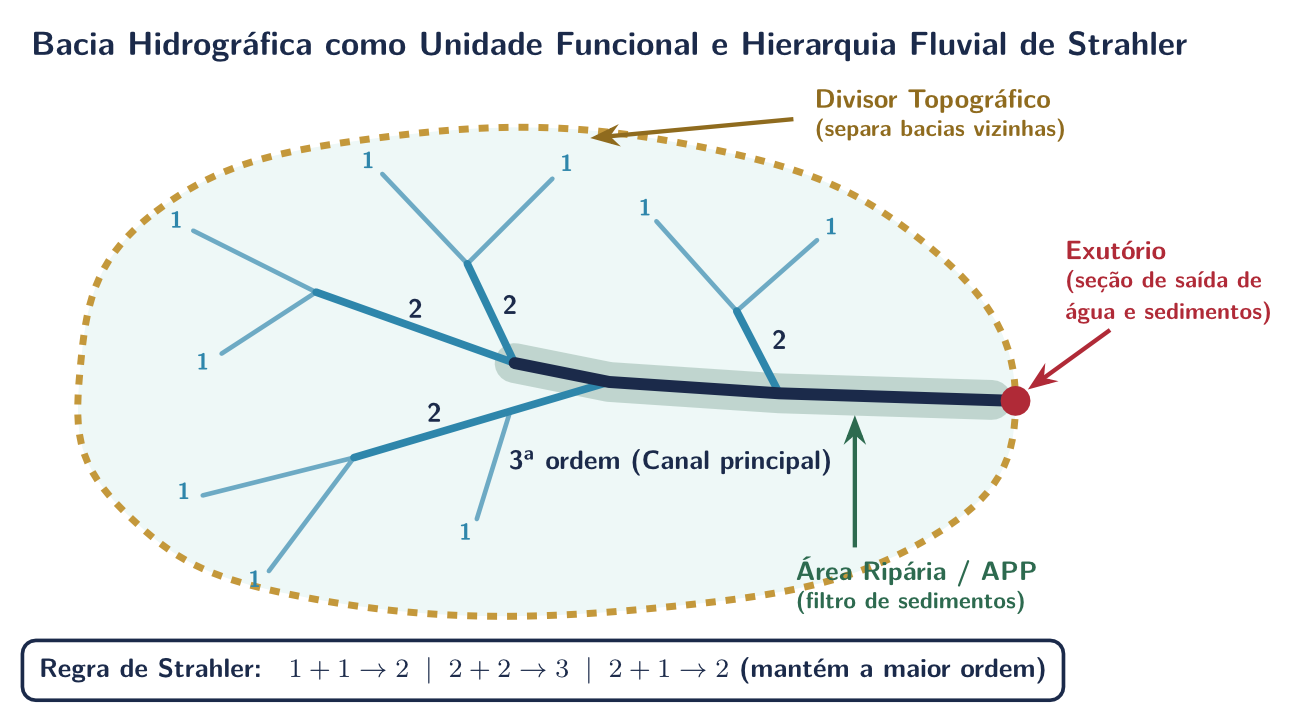
\includegraphics[keepaspectratio]{capitulos/../img/fig05_bacia_hidrografica_strahler.png}}

}

\caption{\label{fig-bacia_strahler}Representação esquemática de uma
bacia hidrográfica como unidade funcional, destacando divisor
topográfico, áreas ripárias (APP), exutório e aplicação da Hierarquia
Fluvial de Strahler (3ª ordem).}

\end{figure}%

Além da ordem hierárquica, a geometria espacial da rede, chamada
\textbf{padrão de drenagem}, oferece pistas imediatas sobre geologia e
relevo,

\textbf{Dendrítico (arborescente).} Lembra galhos de árvore, típico de
rochas com resistência relativamente homogênea à erosão (como granitos e
gnaisses pouco fraturados ou coberturas sedimentares horizontais).
\textbf{Retangular ou treliça.} Confluências próximas a \(90^\circ\),
denunciando forte controle estrutural por falhas, fraturas ou
dobramentos (frequente em setores serranos da Chapada Diamantina).
\textbf{Paralelo.} Canais alongados e quase paralelos entre si,
característicos de vertentes com declividade acentuada e uniforme.
\textbf{Radial.} Canais divergem de um ponto alto central (morros
isolados, domos) ou convergem para uma depressão fechada.

\subsection{Morfometria de Bacias
Hidrográficas}\label{morfometria-de-bacias-hidrogruxe1ficas}

A \textbf{análise morfométrica} consiste em traduzir as características
geométricas, lineares, areais e hipsométricas de uma bacia em índices
numéricos objetivos (Christofoletti, 1981; Villela; Mattos, 1975). Esses
índices permitem diagnosticar a permeabilidade do substrato, a
velocidade de resposta às chuvas, a propensão natural a enchentes e o
potencial energético para erosão e transporte de sedimentos. A seguir,
examinamos os cinco parâmetros essenciais exigidos no Plano CHF662.

\subsubsection{\texorpdfstring{Densidade de Drenagem
(\(D_d\))}{Densidade de Drenagem (D\_d)}}\label{densidade-de-drenagem-d_d}

\subsection{\texorpdfstring{Densidade de Drenagem, \(D_d\) (Horton,
1945)}{Densidade de Drenagem, D\_d (Horton, 1945)}}\label{densidade-de-drenagem-d_d-horton-1945}

\textbf{Origem e finalidade.} Proposta por Robert E. Horton (1945), a
Densidade de Drenagem expressa o comprimento médio de canais fluviais
por unidade de área da bacia. Ela indica o grau de desenvolvimento e
eficiência do sistema de escoamento superficial, refletindo a interação
entre permeabilidade do solo/rocha, clima, declividade e cobertura
vegetal.

\textbf{Equação,}

\[
D_d = \frac{L_t}{A}
\]

\textbf{Variáveis e unidades,}

\(D_d\), densidade de drenagem, expressa em \(\text{km}/\text{km}^2\)
(ou \(\text{km}^{-1}\)). \(L_t\), comprimento total somado de todos os
cursos d'água da bacia, em \(\text{km}\). \(A\), área total de drenagem
da bacia, em \(\text{km}^2\).

\textbf{Exemplo numérico completo.} Uma microbacia possui área
\(A = 25,0\text{ km}^2\) e somatório dos canais mapeados igual a
\(L_t = 45,0\text{ km}\).

\[
D_d = \frac{45{,}0\text{ km}}{25{,}0\text{ km}^2} = 1{,}80\text{ km}/\text{km}^2.
\]

\textbf{Interpretação.} Valor intermediário, compatível com drenagem
moderada a boa, onde parte da água infiltra nos solos e parte escoa
rapidamente pelos canais.

Em termos ambientais, valores baixos de \(D_d\)
(\(< 0,5\text{ km}/\text{km}^2\)) associam-se a rochas e solos muito
permeáveis (como arenitos profundos e Latossolos arenosos), relevos
planos e elevada infiltração. Valores elevados
(\(> 2,0\text{ km}/\text{km}^2\), conforme a
Tabela~\hyperref[tbl-morfometria_interpretacao]{morfometria limiares})
ocorrem em substratos pouco permeáveis (como rochas cristalinas
fraturadas com solos rasos no Semiárido), encostas íngremes e regimes de
chuvas concentradas, indicando rápida geração de escoamento superficial
e maior dissecação erosiva. Um cuidado metodológico indispensável é que
\(D_d\) depende da \textbf{escala cartográfica}, mapas mais detalhados
(1,10.000) registram canais de 1ª ordem efêmeros que desaparecem em
cartas menores (1,100.000), portanto só se devem comparar valores de
\(D_d\) obtidos na mesma escala!

\subsubsection{\texorpdfstring{Índices de Forma, Coeficiente de
Compacidade (\(K_c\)) e Índice de Circularidade
(\(I_c\))}{Índices de Forma, Coeficiente de Compacidade (K\_c) e Índice de Circularidade (I\_c)}}\label{uxedndices-de-forma-coeficiente-de-compacidade-k_c-e-uxedndice-de-circularidade-i_c}

A forma geométrica em planta de uma bacia controla diretamente o
comportamento das cheias no exutório. Em uma bacia próxima a um círculo,
todos os tributários percorrem distâncias parecidas até o exutório,
fazendo com que os picos de vazão cheguem simultaneamente (elevando o
risco de enchentes rápidas). Em uma bacia estreita e alongada, as águas
das cabeceiras levam muito mais tempo para alcançar o exutório do que as
águas do baixo curso, distribuindo a vazão no tempo e atenuando o pico
de cheia.

\subsection{\texorpdfstring{Coeficiente de Compacidade (\(K_c\)) e
Índice de Circularidade
(\(I_c\))}{Coeficiente de Compacidade (K\_c) e Índice de Circularidade (I\_c)}}\label{coeficiente-de-compacidade-k_c-e-uxedndice-de-circularidade-i_c}

\textbf{Origem geométrica e finalidade.} Ambos comparam a geometria da
bacia com a de um círculo perfeito (a figura de menor perímetro para uma
dada área), quantificando a tendência natural à concentração de
enxurradas.

\textbf{Coeficiente de Compacidade (Índice de Gravelius, \(K_c\)).}
Razão entre o perímetro real da bacia (\(P\)) e o perímetro de um
círculo que possua exatamente a mesma área (\(A\)). Como a área de um
círculo é \(A = \pi r^2\), seu raio é \(r = \sqrt{A/\pi}\) e seu
perímetro é
\(P_c = 2\pi r = 2\sqrt{\pi}\sqrt{A} \approx 3,5449\sqrt{A}\). Logo,

\[
K_c = \frac{P}{P_c} = \frac{1}{2\sqrt{\pi}}\cdot \frac{P}{\sqrt{A}} \approx 0{,}2821 \cdot \frac{P}{\sqrt{A}} \;\;\Longrightarrow\;\; K_c = 0{,}28 \cdot \frac{P}{\sqrt{A}}
\]

Na prática hidrológica clássica (Villela; Mattos, 1975), adota-se a
constante arredondada \(0,28\). Como nenhuma forma fechada plana tem
perímetro menor que o círculo de mesma área, tem-se sempre \(K_c \ge 1\)
(adimensional). Quanto mais próximo de \(1,0\), mais circular é a bacia
e maior a propensão a picos de cheia.

\textbf{Índice de Circularidade (Índice de Miller, 1953, \(I_c\)).}
Razão entre a área real da bacia (\(A\)) e a área de um círculo que
possua o mesmo perímetro (\(P\)). Como um círculo de perímetro \(P\) tem
raio \(r = P/(2\pi)\) e área \(A_c = \pi r^2 = \frac{P^2}{4\pi}\),
obtém-se,

\[
I_c = \frac{A}{A_c} = \frac{4\pi \cdot A}{P^2} \approx \frac{12{,}5664 \cdot A}{P^2} \;\;\Longrightarrow\;\; I_c = \frac{12{,}57 \cdot A}{P^2}
\]

O índice \(I_c\) é adimensional e varia no intervalo \(0 < I_c \le 1\).
Quanto mais próximo de \(1,0\), mais circular a bacia (note a relação
inversa, \(I_c \approx 1 / K_c^2\)).

\textbf{Variáveis e unidades,} \(A\) em \(\text{km}^2\) e \(P\) em
\(\text{km}\) (ou \(A\) em \(\text{m}^2\) e \(P\) em \(\text{m}\),
mantendo compatibilidade).

\textbf{Exemplo numérico completo.} Para a mesma microbacia com
\(A = 25,0\text{ km}^2\) e \(P = 24,0\text{ km}\),

\[
\begin{aligned}
K_c &= 0{,}28 \cdot \frac{24{,}0}{\sqrt{25{,}0}} = 0{,}28 \cdot \frac{24{,}0}{5{,}0} = 0{,}28 \cdot 4{,}80 = 1{,}344 \approx 1{,}34 \\
I_c &= \frac{12{,}57 \cdot 25{,}0}{(24{,}0)^2} = \frac{314{,}25}{576{,}0} \approx 0{,}5456 \approx 0{,}55.
\end{aligned}
\]

\textbf{Interpretação.} Com \(K_c = 1,34\) (entre \(1,25\) e \(1,50\)) e
\(I_c = 0,55\) (próximo a \(0,51\)), a bacia apresenta forma
ovalada/mediana, com suscetibilidade moderada a enchentes sob condições
naturais.

\subsubsection{\texorpdfstring{Índices de Relevo, Amplitude Altimétrica
(\(H_m\)) e Relação de Relevo
(\(R_r\))}{Índices de Relevo, Amplitude Altimétrica (H\_m) e Relação de Relevo (R\_r)}}\label{uxedndices-de-relevo-amplitude-altimuxe9trica-h_m-e-relauxe7uxe3o-de-relevo-r_r}

A energia potencial disponível para movimentar água e sedimentos das
cabeceiras ao exutório depende do desnível topográfico distribuído ao
longo do comprimento da bacia.

\subsection{\texorpdfstring{Amplitude Altimétrica (\(H_m\)) e Relação de
Relevo (\(R_r\), Schumm,
1956)}{Amplitude Altimétrica (H\_m) e Relação de Relevo (R\_r, Schumm, 1956)}}\label{amplitude-altimuxe9trica-h_m-e-relauxe7uxe3o-de-relevo-r_r-schumm-1956}

\textbf{Origem e finalidade.} A Amplitude Altimétrica (\(H_m\)) mede a
diferença vertical total da bacia; porém, isoladamente, ela não informa
se esse desnível ocorre em \(2\text{ km}\) (encostas abruptas) ou em
\(200\text{ km}\) (planície suave). Para resolver isso, Stanley Schumm
(1956) definiu a Relação de Relevo (\(R_r\)), que relaciona o desnível
total ao comprimento axial da bacia, funcionando como um indicador
direto da declividade geral média e do potencial erosivo e de transporte
de sedimentos.

\textbf{Equações,}

\[
H_m = H_{\max} - H_{\min} \qquad\text{e}\qquad R_r = \frac{H_m}{L}
\]

\textbf{Variáveis e unidades (atenção redobrada!),}

\(H_{\max}\) e \(H_{\min}\), altitude máxima no divisor e altitude
mínima no exutório, em metros (\(\text{m}\)). \(H_m\), amplitude
altimétrica, em metros (\(\text{m}\)). \(L\), comprimento axial da bacia
(paralelo ao canal principal, do exutório ao divisor), em \(\text{km}\)
ou \(\text{m}\). \(R_r\), pode ser expresso em \(\text{m}/\text{km}\)
(quando \(H_m\) está em \(\text{m}\) e \(L\) em \(\text{km}\)) ou na
forma adimensional \(\text{m}/\text{m}\) (convertendo \(L\) para metros,
\(L_{\text{m}} = L_{\text{km}} \times 1.000\)).

\textbf{Exemplo numérico completo.} Se nossa microbacia tem
\(H_{\max} = 420\text{ m}\), \(H_{\min} = 220\text{ m}\) e
\(L = 8,0\text{ km}\),

\[
\begin{aligned}
H_m &= 420 - 220 = 200\text{ m} \\
R_r &= \frac{200\text{ m}}{8{,}0\text{ km}} = 25{,}0\text{ m}/\text{km} = \frac{200\text{ m}}{8.000\text{ m}} = 0{,}025\text{ m}/\text{m}\;\; (2{,}5\%).
\end{aligned}
\]

\textbf{Interpretação.} Em média, o relevo cai \(25\text{ m}\) a cada
quilômetro percorrido ao longo do eixo principal, um gradiente moderado
que requer atenção conservacionista nas cabeceiras mais inclinadas.

A Tabela~\hyperref[tbl-morfometria_interpretacao]{morfometria
interpretacao} reúne faixas usuais de referência utilizadas em
diagnósticos ambientais para interpretar rapidamente \(D_d\), \(K_c\),
\(I_c\) e \(R_r\).

\begin{longtable}[]{@{}
  >{\raggedright\arraybackslash}p{(\linewidth - 4\tabcolsep) * \real{0.3333}}
  >{\raggedright\arraybackslash}p{(\linewidth - 4\tabcolsep) * \real{0.3333}}
  >{\raggedright\arraybackslash}p{(\linewidth - 4\tabcolsep) * \real{0.3333}}@{}}
\caption{Síntese interpretativa dos principais índices morfométricos de
bacias
hidrográficas.}\label{tbl-morfometria_interpretacao}\tabularnewline
\toprule\noalign{}
\begin{minipage}[b]{\linewidth}\raggedright
Índice
\end{minipage} & \begin{minipage}[b]{\linewidth}\raggedright
Faixa de referência do exercício
\end{minipage} & \begin{minipage}[b]{\linewidth}\raggedright
Interpretação condicionada ao contexto
\end{minipage} \\
\midrule\noalign{}
\endfirsthead
\toprule\noalign{}
\begin{minipage}[b]{\linewidth}\raggedright
Índice
\end{minipage} & \begin{minipage}[b]{\linewidth}\raggedright
Faixa de referência do exercício
\end{minipage} & \begin{minipage}[b]{\linewidth}\raggedright
Interpretação condicionada ao contexto
\end{minipage} \\
\midrule\noalign{}
\endhead
\bottomrule\noalign{}
\endlastfoot
Densidade de drenagem & Menor que 0,5 km/km² & Menor extensão mapeada de
canais por área. Conferir permeabilidade, relevo e critério de
extração. \\
Densidade de drenagem & De 0,5 a 2,0 km/km² & Condição intermediária no
conjunto de faixas adotado. A comparação exige redes obtidas pelo mesmo
método. \\
Densidade de drenagem & Maior que 2,0 km/km² & Maior extensão de canais
por área. Investigar dissecação, materiais e conectividade do
escoamento. \\
Compacidade & De 1,00 a 1,25 & Forma próxima da circular, considerada
junto à chuva, ao armazenamento e à velocidade do escoamento. \\
Compacidade & De 1,25 a 1,50 & Forma intermediária nas faixas didáticas
adotadas. \\
Compacidade & Maior que 1,50 & Forma mais alongada. A resposta de cheia
permanece dependente das demais condições hidrológicas. \\
Circularidade & Maior que 0,51 & Maior aproximação da forma circular
segundo o limiar de referência utilizado. \\
Circularidade & Até 0,51 & Menor circularidade. Verificar geometria,
delimitação e método de medição do perímetro. \\
Relação de relevo & Menor que 15 m/km & Menor gradiente altimétrico
global na faixa de referência adotada. \\
Relação de relevo & De 15 a 40 m/km & Gradiente intermediário, cuja
distribuição interna precisa ser examinada nas vertentes. \\
Relação de relevo & Maior que 40 m/km & Maior gradiente global,
interpretado junto à geometria, aos materiais e à cobertura. \\
\end{longtable}

\subsection{Áreas Ripárias, Conectividade Hidrossedimentológica e
Mudanças de Uso da
Terra}\label{uxe1reas-ripuxe1rias-conectividade-hidrossedimentoluxf3gica-e-mudanuxe7as-de-uso-da-terra}

Os índices morfométricos descrevem a arquitetura física ``estática'' (ou
de evolução lenta) da bacia, mas a resposta ambiental real depende
criticamente da cobertura vegetal e do manejo do solo nas vertentes e
nas margens fluviais.

\subsubsection{Áreas Ripárias e Zonas
Tampão}\label{uxe1reas-ripuxe1rias-e-zonas-tampuxe3o}

As \textbf{áreas ripárias} (matas ciliares, galerias e várzeas
marginais, juridicamente protegidas como Áreas de Preservação
Permanente, APPs, pelo Código Florestal, Lei nº 12.651/2012) constituem
a interface ecossistêmica entre a vertente terrestre e o canal fluvial.
Elas desempenham quatro funções ambientais insubstituíveis,

\textbf{Filtragem de sedimentos e agroquímicos.} A serapilheira e os
caules aumentam a rugosidade superficial, desacelerando a enxurrada
proveniente das vertentes e retendo solo erodido antes que atinja o
leito do rio. \textbf{Estabilização geotécnica das margens.} O
entrelaçamento das raízes eleva a resistência ao cisalhamento dos
barrancos, reduzindo o solapamento marginal e o alargamento erosivo do
canal. \textbf{Regulação térmica e ecológica.} O sombreamento mantém
temperaturas mais amenas na água, preserva teores de oxigênio dissolvido
e fornece matéria orgânica e abrigo para a biota aquática.

\textbf{Recarga e amortecimento de cheias.} Solos ripários porosos atuam
como esponjas, armazenando água nos períodos chuvosos e liberando-a
gradualmente para manter o fluxo de base nos períodos secos.

\subsubsection{Conectividade
Hidrossedimentológica}\label{conectividade-hidrossedimentoluxf3gica}

Na geomorfologia fluvial contemporânea, denomina-se
\textbf{conectividade hidrossedimentológica} a eficiência com que água e
partículas de solo mobilizadas nas vertentes conseguem efetivamente
viajar até a rede de canais e atingir o exutório (Brierley; Fryirs,
2005). Ela possui duas dimensões,

\textbf{Conectividade estrutural.} Continuidade física dos caminhos de
fluxo (declividade, presença de ravinas, estradas rurais mal drenadas ou
galerias pluviais que ligam diretamente a encosta ao rio).
\textbf{Conectividade funcional.} Ativação efetiva desses caminhos
durante eventos chuvosos (por exemplo, um canal efêmero no Semiárido só
se torna funcionalmente conectado após chuvas convectivas intensas que
superam a capacidade de infiltração).

Uma mata ciliar conservada, terraços agrícolas em nível ou paliçadas
permeáveis atuam como \textbf{desconectores} (barreiras ou
\emph{buffers}), interrompendo a chegada de sedimentos ao curso d'água.
Por outro lado, o desmatamento das margens e a abertura de estradas não
pavimentadas morro abaixo funcionam como \textbf{conectores
artificiais}, acelerando o assoreamento de rios e açudes.

\subsubsection{Impactos da Mudança de Uso da Terra, Impermeabilização e
Desmatamento}\label{impactos-da-mudanuxe7a-de-uso-da-terra-impermeabilizauxe7uxe3o-e-desmatamento}

Quando uma microbacia florestada ou coberta por Caatinga preservada é
convertida em pastagem degradada, monocultura sem práticas
conservacionistas ou loteamento urbano pavimentado, ocorre uma alteração
drástica no balanço hídrico local,

\textbf{Queda da interceptação e da infiltração.} A retirada do dossel e
a selagem/pavimentação do solo impedem a entrada da água no perfil
edáfico, elevando o \textbf{coeficiente de escoamento superficial
(\(C\))}, definido como a razão entre o volume escoado na superfície e o
volume total precipitado (tipicamente \(0,10\) a \(0,20\) em florestas e
\(0,65\) a \(0,90\) em áreas urbanas densamente impermeabilizadas).
\textbf{Redução do tempo de concentração e amplificação do pico de
cheia.} A água corre mais rápido sobre asfalto, telhados e solos
compactados, gerando hidrogramas mais agudos e inundações frequentes,
mesmo sem aumento na chuva total, cenário recorrente em microbacias
urbanizadas de Feira de Santana (como cabeceiras do Rio Subaé e do Rio
Jacuípe).

\textbf{Redução da recarga de aquíferos e das vazões de estiagem.} Como
menos água infiltra durante as chuvas, os lençóis freáticos recebem
menor recarga, fazendo com que nascentes sequem ou apresentem vazão
muito reduzida na estação seca.

\subsection{Delimitação, resolução e interpretação
hidrológica}\label{delimitauxe7uxe3o-resoluuxe7uxe3o-e-interpretauxe7uxe3o-hidroluxf3gica}

A posição do exutório condiciona toda a delimitação. Deslocamentos desse
ponto podem incorporar tributários e modificar área, perímetro e
comprimento do canal principal. O registro de suas coordenadas e a
inspeção do modelo de elevação são necessários para que outra pessoa
possa repetir o procedimento.

A densidade de drenagem também responde ao critério utilizado para
iniciar os canais. Um limiar menor de área de contribuição tende a
produzir uma rede mais extensa e, consequentemente, maior densidade. A
comparação entre bacias requer a mesma base, a mesma resolução e um
critério de extração compatível, acompanhado de verificação cartográfica
e de campo.

Forma circular pode favorecer a chegada de contribuições em intervalos
próximos, dependendo da distribuição da chuva e da velocidade do
escoamento. A previsão de cheia exige ainda intensidade e duração da
precipitação, umidade antecedente, armazenamento e capacidade dos
canais. Índices de forma devem sustentar uma interpretação condicionada
a esses fatores.

O coeficiente de compacidade possui expressão geométrica exata dada pela
razão entre o perímetro observado e o perímetro do círculo de mesma
área. O fator \(1/(2\sqrt{\pi})\) vale aproximadamente 0,2821. A
aproximação por 0,28 introduz pequena diferença perto do limite circular
e deve ser reconhecida ao conferir resultados próximos de 1.

\section{Etapa 4 - Exemplos
resolvidos}\label{etapa-4---exemplos-resolvidos-6}

\subsection{Exemplo 7.1 - Hierarquia Fluvial de Strahler em uma
Microbacia de Cabeceira (Nível
Básico)}\label{exemplo-7.1---hierarquia-fluvial-de-strahler-em-uma-microbacia-de-cabeceira-nuxedvel-buxe1sico}

\textbf{Situação analisada.} Durante o mapeamento hidrográfico de uma
microbacia afluente do Rio Jacuípe (BA), uma equipe de Geografia
identificou a seguinte estrutura de drenagem de montante para jusante,
(a) dois córregos sem afluentes (\(C_1\) e \(C_2\)) unem-se formando o
trecho \(T_1\); (b) dois outros córregos sem afluentes (\(C_3\) e
\(C_4\)) unem-se formando o trecho \(T_2\); (c) um córrego sem afluentes
(\(C_5\)) desemboca no trecho \(T_2\), originando o trecho \(T_3\); (d)
os trechos \(T_1\) e \(T_3\) encontram-se, formando o canal \(T_4\); (e)
finalmente, dois novos córregos sem afluentes (\(C_6\) e \(C_7\))
unem-se formando o trecho \(T_5\), que desemboca em \(T_4\), gerando o
canal principal \(T_6\) até o exutório.

\textbf{Dados disponíveis.} Sete canais de cabeceira sem tributários
(\(C_1\) a \(C_7\)) e cinco pontos de confluência sequenciais até o
exutório (\(T_6\)).

\textbf{Problema a resolver.} Determinar a ordem de Strahler de cada
trecho (\(T_1\) a \(T_6\)) e a ordem final da microbacia.

\textbf{Fundamento da análise.} Aplicação sequencial das três regras da
Hierarquia Fluvial de Strahler (1952), nascentes sem afluentes \(= 1\);
encontro \(n + n \to n + 1\); encontro \(n + m \to \max(n, m)\).

\textbf{Desenvolvimento.}

\textbf{Canais sem afluentes,} \(C_1, C_2, C_3, C_4, C_5, C_6\) e
\(C_7\) são todos de \textbf{1ª ordem}. \textbf{Trecho \(T_1\).}
Encontro de \(C_1\) (1ª) com \(C_2\) (1ª) \(\Rightarrow 1 + 1 \to\)
\textbf{2ª ordem}. \textbf{Trecho \(T_2\).} Encontro de \(C_3\) (1ª) com
\(C_4\) (1ª) \(\Rightarrow 1 + 1 \to\) \textbf{2ª ordem}. \textbf{Trecho
\(T_3\).} Encontro de \(T_2\) (2ª) com \(C_5\) (1ª). Como as ordens são
diferentes, mantém-se a maior \(\Rightarrow 2 + 1 \to\) \textbf{2ª
ordem}. \textbf{Trecho \(T_4\).} Encontro de \(T_1\) (2ª) com \(T_3\)
(2ª). Como ambos são de 2ª ordem, eleva-se a hierarquia
\(\Rightarrow 2 + 2 \to\) \textbf{3ª ordem}. \textbf{Trecho \(T_5\).}
Encontro de \(C_6\) (1ª) com \(C_7\) (1ª) \(\Rightarrow 1 + 1 \to\)
\textbf{2ª ordem}.

\textbf{Trecho \(T_6\) (exutório).} Encontro de \(T_4\) (3ª) com \(T_5\)
(2ª). Ordens desiguais mantêm a maior \(\Rightarrow 3 + 2 \to\)
\textbf{3ª ordem}.

\textbf{Interpretação do resultado.} \(T_1 = 2^{\text{a}}\),
\(T_2 = 2^{\text{a}}\), \(T_3 = 2^{\text{a}}\), \(T_4 = 3^{\text{a}}\),
\(T_5 = 2^{\text{a}}\), \(T_6 = 3^{\text{a}}\) ordem. Portanto, trata-se
de uma \textbf{microbacia de 3ª ordem}.

\textbf{Condições de validade.} Para surgir uma bacia de 4ª ordem seriam
necessários, no mínimo, dois segmentos de 3ª ordem confluindo entre si
(o que exigiria ao menos quatro canais de 2ª ordem e oito de 1ª ordem
perfeitamente pareados). Com apenas sete canais de 1ª ordem, é
matematicamente impossível ultrapassar a 3ª ordem, confirmando a
consistência da resposta.

\subsection{Exemplo 7.2 - Densidade de Drenagem e Contraste Litológico
(Nível
Básico-Intermediário)}\label{07-bacias-hidrograficas-morfometria-exemplo-7.2.-densidade-de-drenagem-e-contraste-litoluxf3gico-nuxedvel-buxe1sicointermediuxe1rio}

\textbf{Situação analisada.} Em um diagnóstico ambiental comparativo na
Bahia, analisaram-se duas microbacias rurais de mesma área, mapeadas na
mesma escala 1,25.000, a \textbf{Microbacia A}, situada sobre
embasamento cristalino (gnaisses) com solos rasos no Semiárido, e a
\textbf{Microbacia B}, situada sobre bacia sedimentar arenosa com solos
profundos e bem drenados.

\textbf{Dados disponíveis.} Microbacia A, \(A_A = 16,0\text{ km}^2\) e
\(L_{tA} = 41,6\text{ km}\). Microbacia B, \(A_B = 16,0\text{ km}^2\) e
\(L_{tB} = 12,8\text{ km}\).

\textbf{Problema a resolver.} Calcular a Densidade de Drenagem (\(D_d\))
de cada microbacia e explicar a relação entre os resultados, a
permeabilidade do terreno e a geração de escoamento superficial.

\textbf{Fundamento da análise.} Aplicação da equação de Horton
(\(D_d = L_t / A\)) e interpretação hidrogeomorfológica comparativa.

\textbf{Desenvolvimento.}

\textbf{Microbacia A (cristalino),}

\[
D_{dA} = \frac{L_{tA}}{A_A} = \frac{41{,}6\text{ km}}{16{,}0\text{ km}^2} = 2{,}60\text{ km}/\text{km}^2.
\]

. \textbf{Microbacia B (sedimentar arenoso),}

\[
D_{dB} = \frac{L_{tB}}{A_B} = \frac{12{,}8\text{ km}}{16{,}0\text{ km}^2} = 0{,}80\text{ km}/\text{km}^2.
\]

. \textbf{Razão comparativa,}

\[
\frac{D_{dA}}{D_{dB}} = \frac{2{,}60}{0{,}80} = 3{,}25.
\]

.

\textbf{Interpretação do resultado.}
\(D_{dA} = 2,60\text{ km}/\text{km}^2\) (drenagem alta) e
\(D_{dB} = 0,80\text{ km}/\text{km}^2\) (drenagem regular/baixa). A
Microbacia A possui densidade de drenagem \(3,25\) vezes maior que a
Microbacia B.

\textbf{Condições de validade.} O resultado faz pleno sentido ambiental,
rochas cristalinas pouco permeáveis e solos rasos (Microbacia A) limitam
a infiltração profunda, forçando grande parte da chuva a escoar em
superfície e entalhar uma rede densa de canais. Já os arenitos e solos
profundos (Microbacia B) favorecem a infiltração e recarga subterrânea,
exigindo menos canais superficiais por \(\text{km}^2\). Como ambas foram
mapeadas na escala 1,25.000, a comparação é metodologicamente válida.

\subsection{\texorpdfstring{Exemplo 7.3 - Forma da Bacia (\(K_c\) e
\(I_c\)) e Suscetibilidade a Enchentes (Nível
Intermediário)}{Exemplo 7.3 - Forma da Bacia (K\_c e I\_c) e Suscetibilidade a Enchentes (Nível Intermediário)}}\label{exemplo-7.3---forma-da-bacia-k_c-e-i_c-e-suscetibilidade-a-enchentes-nuxedvel-intermediuxe1rio}

\textbf{Situação analisada.} A prefeitura de um município baiano precisa
priorizar obras de macrodrenagem e proteção de margens entre duas
sub-bacias periurbanas de mesma área total (\(36,0\text{ km}^2\)), a
\textbf{Bacia X}, de contorno mais arredondado, e a \textbf{Bacia Y},
encaixada em um vale estreito e alongado.

\textbf{Dados disponíveis.} Bacia X, \(A_X = 36,0\text{ km}^2\) e
\(P_X = 24,0\text{ km}\). Bacia Y, \(A_Y = 36,0\text{ km}^2\) e
\(P_Y = 36,0\text{ km}\).

\textbf{Problema a resolver.} Calcular o Coeficiente de Compacidade
(\(K_c\)) e o Índice de Circularidade (\(I_c\)) de ambas as bacias e
indicar qual delas apresenta maior suscetibilidade natural a picos
rápidos de cheia.

\textbf{Fundamento da análise.} Cálculo de
\(K_c = 0,28 \cdot \frac{P}{\sqrt{A}}\) e
\(I_c = \frac{12,57 \cdot A}{P^2}\), seguido de classificação pela
Tabela~\hyperref[tbl-morfometria_interpretacao]{morfometria
interpretacao}.

\textbf{Desenvolvimento.}

\textbf{Raiz quadrada da área (comum às duas bacias),}
\(\sqrt{36,0} = 6,0\text{ km}\). \textbf{Bacia X,}

\[
\begin{aligned}
K_{cX} &= 0{,}28 \cdot \frac{24{,}0}{6{,}0} = 0{,}28 \cdot 4{,}0 = 1{,}12 \\
I_{cX} &= \frac{12{,}57 \cdot 36{,}0}{(24{,}0)^2} = \frac{452{,}52}{576{,}0} \approx 0{,}7856 \approx 0{,}79.
\end{aligned}
\]

. \textbf{Bacia Y,}

\[
\begin{aligned}
K_{cY} &= 0{,}28 \cdot \frac{36{,}0}{6{,}0} = 0{,}28 \cdot 6{,}0 = 1{,}68 \\
I_{cY} &= \frac{12{,}57 \cdot 36{,}0}{(36{,}0)^2} = \frac{12{,}57}{36{,}0} \approx 0{,}3492 \approx 0{,}35.
\end{aligned}
\]

.

\textbf{Interpretação do resultado.} Bacia X, \(K_c = 1,12\) e
\(I_c = 0,79\) (forma tendendo à circular, \textbf{alta suscetibilidade
a enchentes}). Bacia Y, \(K_c = 1,68\) e \(I_c = 0,35\) (forma alongada,
\textbf{baixa suscetibilidade natural a picos concentrados}). A Bacia X
deve receber prioridade nas medidas preventivas contra cheias rápidas.

\textbf{Condições de validade.} Verificamos a coerência matemática entre
os dois índices, para a Bacia X,
\(1 / K_{cX}^2 = 1 / (1,12)^2 = 1 / 1,2544 \approx 0,80 \approx I_{cX}\)
(a pequena diferença decorre do arredondamento de \(0,2821\) para
\(0,28\)). Além disso, ambos respeitam os limites geométricos
\(K_c \ge 1\) e \(I_c \le 1\).

\subsection{\texorpdfstring{Exemplo 7.4 - Amplitude Altimétrica
(\(H_m\)) e Relação de Relevo (\(R_r\)) em Cabeceiras Contrastantes
(Nível
Intermediário)}{Exemplo 7.4 - Amplitude Altimétrica (H\_m) e Relação de Relevo (R\_r) em Cabeceiras Contrastantes (Nível Intermediário)}}\label{exemplo-7.4---amplitude-altimuxe9trica-h_m-e-relauxe7uxe3o-de-relevo-r_r-em-cabeceiras-contrastantes-nuxedvel-intermediuxe1rio}

\textbf{Situação analisada.} Para avaliar o potencial energético de
erosão e transporte de sedimentos, comparam-se duas microbacias de mesmo
comprimento axial (\(L = 6,0\text{ km}\)), uma situada nas cabeceiras
serranas da \textbf{Chapada Diamantina} e outra localizada em setor
aplainado do \textbf{Planalto Sertanejo}.

\textbf{Dados disponíveis.} Chapada Diamantina,
\(H_{\max} = 960\text{ m}\), \(H_{\min} = 480\text{ m}\),
\(L = 6,0\text{ km}\). Planalto Sertanejo, \(H_{\max} = 360\text{ m}\),
\(H_{\min} = 240\text{ m}\), \(L = 6,0\text{ km}\).

\textbf{Problema a resolver.} Calcular \(H_m\) e \(R_r\) (em
\(\text{m}/\text{km}\) e em \(\text{m}/\text{m}\)) para ambas as
unidades e interpretar suas implicações geomorfológicas.

\textbf{Fundamento da análise.} Aplicação de
\(H_m = H_{\max} - H_{\min}\) e \(R_r = H_m / L\), com conversão
cuidadosa de \(L\) de quilômetros para metros
(\(6,0\text{ km} = 6.000\text{ m}\)) na forma adimensional.

\textbf{Desenvolvimento.}

\textbf{Cabeceira da Chapada Diamantina,}

\[
\begin{aligned}
H_{m1} &= 960 - 480 = 480\text{ m} \\
R_{r1} &= \frac{480\text{ m}}{6{,}0\text{ km}} = 80{,}0\text{ m}/\text{km} \\
R_{r1,\text{adim}} &= \frac{480\text{ m}}{6.000\text{ m}} = 0{,}080\text{ m}/\text{m} \;\; (8{,}0\%).
\end{aligned}
\]

. \textbf{Planalto Sertanejo,}

\[
\begin{aligned}
H_{m2} &= 360 - 240 = 120\text{ m} \\
R_{r2} &= \frac{120\text{ m}}{6{,}0\text{ km}} = 20{,}0\text{ m}/\text{km} \\
R_{r2,\text{adim}} &= \frac{120\text{ m}}{6.000\text{ m}} = 0{,}020\text{ m}/\text{m} \;\; (2{,}0\%).
\end{aligned}
\]

.

\textbf{Interpretação do resultado.} Chapada Diamantina,
\(H_m = 480\text{ m}\) e \(R_r = 80,0\text{ m}/\text{km}\)
(\(0,080\text{ m}/\text{m}\)). Planalto Sertanejo,
\(H_m = 120\text{ m}\) e \(R_r = 20,0\text{ m}/\text{km}\)
(\(0,020\text{ m}/\text{m}\)). A microbacia serrana possui energia de
relevo \(4\) vezes superior.

\textbf{Condições de validade.} A mesma distância horizontal
(\(6\text{ km}\)) acomoda um desnível \(4\) vezes maior na Chapada,
gerando velocidades de escoamento bem mais elevadas, maior capacidade de
transporte de blocos e cascalhos e maior sensibilidade a ravinas e
movimentos de massa caso a vegetação seja removida.

\subsection{Exemplo 7.5 - Impacto Hidrológico da Impermeabilização
Urbana em uma Microbacia (Nível
Avançado)}\label{exemplo-7.5---impacto-hidroluxf3gico-da-impermeabilizauxe7uxe3o-urbana-em-uma-microbacia-nuxedvel-avanuxe7ado}

\textbf{Situação analisada.} Uma microbacia periurbana de
\(4,0\text{ km}^2\) na borda de expansão de Feira de Santana era
originalmente coberta por vegetação nativa e áreas ripárias conservadas,
apresentando coeficiente médio de escoamento superficial \(C_1 = 0,15\).
Após a implantação de loteamentos pavimentados, canalização de córregos
e supressão da mata ciliar, o coeficiente subiu para \(C_2 = 0,75\).
Considere uma chuva intensa de \(P_{\text{chuva}} = 60\text{ mm}\).

\textbf{Dados disponíveis.}
\(A = 4,0\text{ km}^2 = 4.000.000\text{ m}^2\);
\(P_{\text{chuva}} = 60\text{ mm} = 0,060\text{ m}\); \(C_1 = 0,15\);
\(C_2 = 0,75\).

\textbf{Problema a resolver.} Calcular o volume total de água
precipitado sobre a microbacia, o volume de escoamento superficial
gerado antes e depois da urbanização, a diferença absoluta e relativa, e
explicar os reflexos sobre a conectividade hidrossedimentológica.

\textbf{Fundamento da análise.} Cálculo volumétrico direto do balanço
superficial, \(V_{\text{prec}} = P_{\text{chuva}} \cdot A\) e
\(V_{\text{esc}} = C \cdot V_{\text{prec}}\), seguido de análise
ambiental integrada.

\textbf{Desenvolvimento.}

\textbf{Conversão de unidades,}

\[
A = 4{,}0 \times 1.000.000\text{ m}^2 = 4.000.000\text{ m}^2, \qquad P_{\text{chuva}} = \frac{60}{1.000}\text{ m} = 0{,}060\text{ m}.
\]

. \textbf{Volume total precipitado na microbacia,}

\[
V_{\text{prec}} = 0{,}060\text{ m} \times 4.000.000\text{ m}^2 = 240.000\text{ m}^3.
\]

. \textbf{Volume de escoamento superficial no cenário conservado
(\(C_1 = 0,15\)),}

\[
V_{\text{esc},1} = 0{,}15 \times 240.000\text{ m}^3 = 36.000\text{ m}^3.
\]

(Os outros \(204.000\text{ m}^3\), equivalentes a \(85\%\), foram
retidos por interceptação, depressões e infiltração.). \textbf{Volume de
escoamento superficial no cenário impermeabilizado (\(C_2 = 0,75\)),}

\[
V_{\text{esc},2} = 0{,}75 \times 240.000\text{ m}^3 = 180.000\text{ m}^3.
\]

. \textbf{Aumento absoluto e fator multiplicador,}

\[
\Delta V_{\text{esc}} = 180.000 - 36.000 = 144.000\text{ m}^3, \qquad \frac{V_{\text{esc},2}}{V_{\text{esc},1}} = \frac{180.000}{36.000} = 5\text{ vezes (}+400\%\text{)}.
\]

.

\textbf{Interpretação do resultado.} O escoamento superficial saltou de
\(36.000\text{ m}^3\) para \(180.000\text{ m}^3\), um acréscimo de
\(144.000\text{ m}^3\) (cinco vezes o volume original) para a mesma
chuva de \(60\text{ mm}\).

\textbf{Condições de validade.} Note que \(144.000\text{ m}^3\)
correspondem a cerca de \(58\) piscinas olímpicas (\(2.500\text{ m}^3\)
cada) lançadas abruptamente no canal em poucas horas. A supressão da
mata ciliar e a canalização eliminam os desconectores naturais, elevam
ao máximo a conectividade hidrossedimentológica artificial e provocam
alagamentos a jusante, erosão de margens e redução severa da recarga
subterrânea.

\section{Etapa 5 - Erros de
interpretação}\label{etapa-5---erros-de-interpretauxe7uxe3o-6}

\subsection{\texorpdfstring{Erro 1, Somar ordens diferentes na
Hierarquia de Strahler
(\(2 + 1 = 3\))}{Erro 1, Somar ordens diferentes na Hierarquia de Strahler (2 + 1 = 3)}}\label{erro-1-somar-ordens-diferentes-na-hierarquia-de-strahler-2-1-3}

\textbf{Equívoco frequente.} Acreditar que toda confluência eleva a
ordem do rio, escrevendo incorretamente que um canal de 2ª ordem ao
receber um tributário de 1ª ordem passa a ser de 3ª ordem.

\textbf{Correção técnica.} Na regra de Strahler, a ordem só aumenta
quando se encontram \textbf{dois segmentos de mesma ordem}
(\(1+1 \to 2\), \(2+2 \to 3\)). Quando um canal de ordem inferior
encontra um de ordem superior, prevalece a maior ordem (\(2+1 \to 2\)).

\subsection{\texorpdfstring{Erro 2, Confundir o sentido de interpretação
de \(K_c\) e
\(I_c\)}{Erro 2, Confundir o sentido de interpretação de K\_c e I\_c}}\label{erro-2-confundir-o-sentido-de-interpretauxe7uxe3o-de-k_c-e-i_c}

\textbf{Equívoco frequente.} Afirmar que ``quanto maior o \(K_c\), mais
circular é a bacia e maior o risco de enchentes'', confundindo \(K_c\)
com \(I_c\).

\textbf{Correção técnica,} \(K_c\) e \(I_c\) variam em \textbf{sentidos
opostos}. Quanto mais próxima de um círculo (maior propensão a cheias
rápidas), \textbf{menor} é \(K_c\) (mais próximo de \(1,0\)) e
\textbf{maior} é \(I_c\) (mais próximo de \(1,0\)). Em bacias alongadas,
\(K_c\) cresce (\(> 1,50\)) e \(I_c\) diminui (\(< 0,45\)). Além disso,
um resultado com \(K_c < 1\) ou \(I_c > 1\) denuncia erro de cálculo ou
medição incorreta de área/perímetro.

\subsection{\texorpdfstring{Erro 3, Misturar metros e quilômetros no
cálculo da Relação de Relevo
(\(R_r\))}{Erro 3, Misturar metros e quilômetros no cálculo da Relação de Relevo (R\_r)}}\label{erro-3-misturar-metros-e-quiluxf4metros-no-cuxe1lculo-da-relauxe7uxe3o-de-relevo-r_r}

\textbf{Equívoco frequente.} Dividir \(H_m = 200\text{ m}\) por
\(L = 8\text{ km}\), obter \(25\) e registrar o resultado como
``\(25\text{ m/m}\)'' ou ``\(25\%\)''.

\textbf{Correção técnica.} Ao dividir metros por quilômetros, a unidade
obrigatória é \(\text{m}/\text{km}\) (\(25\text{ m}/\text{km}\)). Para
obter \(R_r\) adimensional (\(\text{m}/\text{m}\)) ou em porcentagem,
converta \(L\) para metros antes de dividir,
\(200\text{ m} / 8.000\text{ m} = 0,025\text{ m}/\text{m} = 2,5\%\).

\subsection{\texorpdfstring{Erro 4, Comparar Densidade de Drenagem
(\(D_d\)) obtida em escalas cartográficas
diferentes}{Erro 4, Comparar Densidade de Drenagem (D\_d) obtida em escalas cartográficas diferentes}}\label{erro-4-comparar-densidade-de-drenagem-d_d-obtida-em-escalas-cartogruxe1ficas-diferentes}

\textbf{Equívoco frequente.} Calcular \(D_d\) de uma bacia a partir de
imagem de alta resolução/carta 1,10.000 e compará-la com o \(D_d\) de
outra bacia extraído de base 1,100.000, concluindo que a primeira é
``muito menos permeável''.

\textbf{Correção técnica.} Bases de escala pequena (1,100.000)
generalizam a rede hidrográfica e omitem a maioria dos canais de 1ª
ordem, subestimando \(L_t\) e \(D_d\). Análises comparativas só são
válidas quando a rede de drenagem de todas as bacias é vetorizada na
mesma escala e sob o mesmo critério de mapeamento.

\section{Etapa 6 - Exercícios de
fixação}\label{etapa-6---exercuxedcios-de-fixauxe7uxe3o-6}

\subsubsection{Nível Básico (Exercícios 1 a
5)}\label{nuxedvel-buxe1sico-exercuxedcios-1-a-5-2}

\begin{enumerate}
\def\labelenumi{\arabic{enumi}.}
\item
  Explique, com base em Botelho e Silva (2004) e Christofoletti (1981),
  por que a bacia hidrográfica é considerada a unidade espacial mais
  adequada para a análise e o planejamento ambiental, diferenciando
  \textbf{divisor topográfico}, \textbf{talvegue} e \textbf{exutório}.
\item
  Uma microbacia rural apresenta área de drenagem
  \(A = 20,0\text{ km}^2\) e comprimento total de canais
  \(L_t = 35,0\text{ km}\). Calcule sua Densidade de Drenagem (\(D_d\))
  e classifique-a conforme a
  Tabela~\hyperref[tbl-morfometria_interpretacao]{morfometria
  interpretacao}.
\item
  Calcule o Coeficiente de Compacidade (\(K_c\)) de uma sub-bacia com
  área \(A = 49,0\text{ km}^2\) e perímetro \(P = 35,0\text{ km}\).
  Indique se sua forma tende à circular, ovalada ou alongada.
\item
  Uma microbacia possui área \(A = 25,0\text{ km}^2\) e perímetro
  \(P = 25,0\text{ km}\). Calcule seu Índice de Circularidade (\(I_c\))
  e avalie sua propensão natural a picos concentrados de enchente.
\item
  Determine a Amplitude Altimétrica (\(H_m\)) e a Relação de Relevo
  (\(R_r\)), em \(\text{m}/\text{km}\) e em \(\text{m}/\text{m}\), para
  uma bacia com \(H_{\max} = 640\text{ m}\), \(H_{\min} = 280\text{ m}\)
  e comprimento axial \(L = 9,0\text{ km}\).
\end{enumerate}

\subsubsection{Nível Intermediário (Exercícios 6 a
10)}\label{nuxedvel-intermediuxe1rio-exercuxedcios-6-a-10-2}

\begin{enumerate}
\def\labelenumi{\arabic{enumi}.}
\setcounter{enumi}{5}
\item
  Compare duas bacias hidrográficas mapeadas na mesma escala (1,25.000),
  ambas com área \(A = 64,0\text{ km}^2\),

  \begin{itemize}
  \item
    \textbf{Bacia M1,} \(P = 32,0\text{ km}\),
    \(L_t = 160,0\text{ km}\), \(H_{\max} = 540\text{ m}\),
    \(H_{\min} = 220\text{ m}\), \(L = 8,0\text{ km}\).
  \item
    \textbf{Bacia M2,} \(P = 48,0\text{ km}\), \(L_t = 51,2\text{ km}\),
    \(H_{\max} = 380\text{ m}\), \(H_{\min} = 220\text{ m}\),
    \(L = 16,0\text{ km}\).
  \end{itemize}

  Calcule \(D_d\), \(K_c\), \(I_c\), \(H_m\) e \(R_r\) para ambas e
  justifique qual delas exige maior cuidado contra cheias rápidas e
  processos erosivos.
\item
  Em uma rede hidrográfica hipotética, quatro pares de canais de 1ª
  ordem formam quatro canais de 2ª ordem (\(A, B, C, D\)). Os canais
  \(A\) e \(B\) se unem formando o trecho \(X\); o canal \(C\) desemboca
  em \(X\) formando o trecho \(Y\); e o canal \(D\) desemboca em \(Y\)
  formando o canal final \(Z\) no exutório. Determine a ordem de
  Strahler de \(X\), \(Y\) e \(Z\) e explique por que a ordem final não
  chegou a 4ª ordem.
\item
  Uma microbacia de \(5,0\text{ km}^2\) sofreu desmatamento e abertura
  de estradas compactadas, elevando seu coeficiente de escoamento
  superficial de \(C_1 = 0,20\) para \(C_2 = 0,70\). Para uma chuva de
  \(50\text{ mm}\), calcule o volume escoado superficialmente (em
  \(\text{m}^3\)) nos dois cenários e o percentual de aumento do
  escoamento.
\item
  Explique a diferença entre \textbf{conectividade estrutural} e
  \textbf{conectividade funcional} em uma bacia hidrográfica do
  Semiárido baiano e dê um exemplo de elemento que atua como
  \emph{conector} e outro que atua como \emph{desconector} de
  sedimentos.
\item
  Por que a supressão de matas ciliares (áreas ripárias) em microbacias
  rurais provoca simultaneamente aumento da turbidez da água,
  assoreamento de reservatórios e instabilidade de margens?
\end{enumerate}

\subsubsection{Questões Objetivas (Exercícios 11 a
15)}\label{questuxf5es-objetivas-exercuxedcios-11-a-15}

\begin{enumerate}
\def\labelenumi{\arabic{enumi}.}
\setcounter{enumi}{10}
\item
  Na Hierarquia Fluvial de Strahler, quando um curso d'água de 3ª ordem
  recebe um afluente de 2ª ordem e, mais a jusante, conflui com outro
  curso d'água de 3ª ordem, as ordens dos segmentos imediatamente após a
  primeira e a segunda confluência serão, respectivamente,

  \begin{enumerate}
  \def\labelenumii{(\Alph{enumii})}
  \item
    4ª ordem e 5ª ordem.
  \item
    3ª ordem e 4ª ordem.
  \item
    3ª ordem e 3ª ordem.
  \item
    5ª ordem e 6ª ordem.
  \item
    2ª ordem e 4ª ordem.
  \end{enumerate}
\item
  Uma bacia hidrográfica apresenta \(A = 100,0\text{ km}^2\),
  \(P = 50,0\text{ km}\), \(L_t = 220,0\text{ km}\),
  \(H_{\max} = 750\text{ m}\), \(H_{\min} = 250\text{ m}\) e
  \(L = 20,0\text{ km}\). Os valores corretos de \(D_d\), \(K_c\) e
  \(R_r\) (em \(\text{m}/\text{km}\)) são, respectivamente,

  \begin{enumerate}
  \def\labelenumii{(\Alph{enumii})}
  \item
    \(2,20\text{ km}/\text{km}^2\); \(1,40\);
    \(25,0\text{ m}/\text{km}\).
  \item
    \(0,45\text{ km}/\text{km}^2\); \(1,40\);
    \(25,0\text{ m}/\text{km}\).
  \item
    \(2,20\text{ km}/\text{km}^2\); \(0,71\);
    \(50,0\text{ m}/\text{km}\).
  \item
    \(2,20\text{ km}/\text{km}^2\); \(1,40\);
    \(0,25\text{ m}/\text{km}\).
  \item
    \(4,40\text{ km}/\text{km}^2\); \(2,80\);
    \(25,0\text{ m}/\text{km}\).
  \end{enumerate}
\item
  Sobre o Coeficiente de Compacidade (\(K_c\)) e o Índice de
  Circularidade (\(I_c\)), assinale a alternativa tecnicamente correta,

  \begin{enumerate}
  \def\labelenumii{(\Alph{enumii})}
  \item
    Uma bacia perfeitamente circular apresenta \(K_c = 0\) e
    \(I_c = 1\).
  \item
    Quanto maior o valor de \(K_c\), maior a tendência da bacia à forma
    circular e maior o risco de cheias súbitas.
  \item
    Valores de \(K_c\) próximos de \(1,0\) e de \(I_c\) próximos de
    \(1,0\) indicam bacia mais circular e maior suscetibilidade a picos
    concentrados de enchente.
  \item
    O valor de \(I_c\) pode assumir qualquer número real positivo
    superior a \(1,0\) em bacias muito alongadas.
  \item
    Os índices \(K_c\) e \(I_c\) dependem exclusivamente da altitude
    máxima e da extensão dos rios, independendo do perímetro.
  \end{enumerate}
\item
  Em relação às áreas ripárias em bacias hidrográficas, é
  \textbf{INCORRETO} afirmar que,

  \begin{enumerate}
  \def\labelenumii{(\Alph{enumii})}
  \item
    Atuam como zonas tampão que retêm parte dos sedimentos e nutrientes
    carreados das vertentes.
  \item
    Contribuem para a estabilização das margens fluviais por meio do
    sistema radicular da vegetação.
  \item
    Aumentam a rugosidade superficial, reduzindo a velocidade do
    escoamento que alcança o canal.
  \item
    Sua remoção eleva a conectividade hidrossedimentológica entre
    encostas agrícolas e o leito fluvial.
  \item
    Sua supressão aumenta a recarga dos aquíferos locais ao eliminar o
    consumo de água por evapotranspiração.
  \end{enumerate}
\item
  A urbanização intensa e sem drenagem sustentável em uma microbacia
  provoca, no hidrograma de cheia medido no exutório,

  \begin{enumerate}
  \def\labelenumii{(\Alph{enumii})}
  \item
    Aumento do tempo de concentração e diminuição do pico de vazão.
  \item
    Redução do volume escoado superficialmente e elevação do fluxo de
    base na estiagem.
  \item
    Redução do tempo de concentração e aumento acentuado da vazão de
    pico.
  \item
    Manutenção inalterada da curva de cheia, pois a área da bacia
    permanece constante.
  \item
    Eliminação da conectividade estrutural entre vertentes e canais.
  \end{enumerate}
\end{enumerate}

\section{Etapa 7 - Questões de
aplicação}\label{etapa-7---questuxf5es-de-aplicauxe7uxe3o-6}

\begin{enumerate}
\def\labelenumi{\arabic{enumi}.}
\setcounter{enumi}{15}
\item
  \textbf{(Questão autoral, estilo ENADE / Licenciatura e Bacharelado em
  Geografia)} Um órgão estadual de meio ambiente avalia o pedido de
  supressão vegetal para expansão agropecuária em uma microbacia de
  cabeceira situada sobre embasamento cristalino no Nordeste brasileiro.
  O relatório técnico apresentou \(D_d = 2,85\text{ km}/\text{km}^2\),
  \(K_c = 1,14\) e \(R_r = 55\text{ m}/\text{km}\). Com base na
  interpretação integrada desses indicadores morfométricos, conclui-se
  que a microbacia apresenta,

  \begin{enumerate}
  \def\labelenumii{(\Alph{enumii})}
  \item
    Substrato muito permeável, forma alongada e relevo plano, com
    baixíssima vulnerabilidade à erosão hídrica.
  \item
    Elevada capacidade de infiltração profunda e lenta resposta
    hidrológica, dispensando faixas ripárias protetoras.
  \item
    Baixa permeabilidade relativa, forma tendente à circular e elevada
    energia de relevo, configurando alta propensão natural a enxurradas
    rápidas e processos erosivos caso a vegetação seja suprimida.
  \item
    Predomínio de deposição sedimentar em planície aluvial ampla, pois
    \(K_c\) próximo de \(1,0\) impede a concentração do escoamento no
    exutório.
  \item
    Incompatibilidade matemática nos dados, visto que uma bacia com
    \(D_d > 2,0\) não pode apresentar \(K_c > 1,0\).
  \end{enumerate}
\item
  \textbf{(Questão autoral, estilo Concurso Analista Ambiental /
  INEMA-BA)} Em um estudo hidrológico para outorga e prevenção de
  inundações, uma sub-bacia foi caracterizada por
  \(A = 81,0\text{ km}^2\), \(P = 36,0\text{ km}\),
  \(L_t = 202,5\text{ km}\), \(H_{\max} = 680\text{ m}\),
  \(H_{\min} = 230\text{ m}\) e \(L = 15,0\text{ km}\). Assinale a
  alternativa que apresenta corretamente os valores de \(D_d\), \(K_c\),
  \(I_c\) e \(R_r\) (em \(\text{m}/\text{m}\)) dessa sub-bacia,

  \begin{enumerate}
  \def\labelenumii{(\Alph{enumii})}
  \item
    \(D_d = 2,50\text{ km}/\text{km}^2\); \(K_c = 1,12\);
    \(I_c = 0,79\); \(R_r = 0,030\text{ m}/\text{m}\).
  \item
    \(D_d = 2,50\text{ km}/\text{km}^2\); \(K_c = 1,12\);
    \(I_c = 0,79\); \(R_r = 30,0\text{ m}/\text{m}\).
  \item
    \(D_d = 0,40\text{ km}/\text{km}^2\); \(K_c = 1,12\);
    \(I_c = 0,79\); \(R_r = 0,030\text{ m}/\text{m}\).
  \item
    \(D_d = 2,50\text{ km}/\text{km}^2\); \(K_c = 1,40\);
    \(I_c = 0,50\); \(R_r = 0,030\text{ m}/\text{m}\).
  \item
    \(D_d = 2,50\text{ km}/\text{km}^2\); \(K_c = 0,89\);
    \(I_c = 1,26\); \(R_r = 0,030\text{ m}/\text{m}\).
  \end{enumerate}
\item
  \textbf{(Questão autoral, estilo Concurso IBAMA / Gestão de Bacias
  Hidrográficas)} Sobre o conceito de conectividade
  hidrossedimentológica aplicado à gestão de bacias hidrográficas,
  analise as afirmativas abaixo,

  \begin{itemize}
  \item
    Estradas vicinais não pavimentadas construídas no sentido da
    declividade atuam como conectores estruturais, canalizando o
    escoamento das vertentes diretamente para os cursos d'água.
  \item
    A recomposição de matas ciliares e a implantação de barreiras de
    retenção de sedimentos reduzem a conectividade entre áreas
    degradadas e o canal principal.
  \item
    Em climas semiáridos, canais efêmeros podem exibir alta
    conectividade estrutural em mapa, mas conectividade funcional
    intermitente, ativada apenas em eventos pluviométricos que superam a
    capacidade de infiltração.
  \end{itemize}

  Está correto o que se afirma em,

  \begin{enumerate}
  \def\labelenumii{(\Alph{enumii})}
  \item
    I, apenas.
  \item
    II, apenas.
  \item
    I e II, apenas.
  \item
    II e III, apenas.
  \item
    I, II e III.
  \end{enumerate}
\end{enumerate}

\subsection{Conexão com a Avaliação Teórica e com o Trabalho Prático
Final}\label{conexuxe3o-com-a-avaliauxe7uxe3o-teuxf3rica-e-com-o-trabalho-pruxe1tico-final}

Na \textbf{Prova Teórica da Semana 10}, os índices morfométricos
raramente são cobrados como contas isoladas, o enunciado exige que você
calcule (\(D_d\), \(K_c\), \(I_c\), \(R_r\)) e \textbf{interprete o
significado ambiental} do número encontrado. No seu \textbf{Trabalho
Prático Final}, extrair esses cinco índices em SIG (QGIS) para a
microbacia escolhida, sempre informando a escala da base cartográfica
utilizada, confere alto rigor técnico à caracterização da área de
estudo.

\section{Etapa 8 - Gabarito
comentado}\label{etapa-8---gabarito-comentado-6}

\subsection{Resoluções e Justificativas, Capítulo
7}\label{resoluuxe7uxf5es-e-justificativas-capuxedtulo-7}

\begin{enumerate}
\def\labelenumi{\arabic{enumi}.}
\item
  \textbf{Conceito e elementos.} A bacia hidrográfica é uma unidade
  espacial natural e sistêmica na qual todos os fluxos de água,
  sedimentos e poluentes das vertentes convergem para um único exutório,
  permitindo relacionar diretamente o uso da terra ao estado dos
  recursos hídricos (Botelho; Silva, 2004; Christofoletti, 1981).
  \emph{Divisor topográfico}, linha de pontos mais altos que separa
  bacias adjacentes; \emph{talvegue}, linha de pontos mais baixos ao
  longo do vale onde se aloja o canal; \emph{exutório}, ponto de menor
  cota do contorno por onde sai toda a drenagem superficial.
\item
  \textbf{Cálculo de \(D_d\),}
  \(D_d = L_t / A = 35,0 / 20,0 = \mathbf{1,75\text{ km}/\text{km}^2}\).
  Classificação, drenagem regular a média (\(0,5\) a
  \(2,0\text{ km}/\text{km}^2\)).
\item
  \textbf{Cálculo de \(K_c\),} \(\sqrt{49,0} = 7,0\text{ km}\). Logo,
  \(K_c = 0,28 \cdot (35,0 / 7,0) = 0,28 \cdot 5,0 = \mathbf{1,40}\).
  Classificação, forma ovalada (\(1,25\) a \(1,50\)), suscetibilidade
  moderada a cheias.
\item
  \textbf{Cálculo de \(I_c\),}
  \(I_c = \frac{12,57 \cdot 25,0}{(25,0)^2} = \frac{12,57}{25,0} = \mathbf{0,5028 \approx 0,50}\).
  Por situar-se no limiar de \(0,51\), indica forma intermediária
  (levemente alongada/ovalada), com propensão moderada a cheias
  concentradas.
\item
  \textbf{Cálculo de \(H_m\) e \(R_r\),}
  \(H_m = 640 - 280 = \mathbf{360\text{ m}}\). Em
  \(\text{m}/\text{km}\),
  \(R_r = 360 / 9,0 = \mathbf{40,0\text{ m}/\text{km}}\). Em
  \(\text{m}/\text{m}\),
  \(L = 9,0\text{ km} = 9.000\text{ m} \Rightarrow R_r = 360 / 9.000 = \mathbf{0,040\text{ m}/\text{m}}\)
  (\(4,0\%\)).
\item
  \textbf{Comparação M1 vs.~M2.} Como \(\sqrt{64,0} = 8,0\),

  \begin{itemize}
  \item
    \textbf{M1,}
    \(D_d = 160,0 / 64,0 = \mathbf{2,50\text{ km}/\text{km}^2}\);
    \(K_c = 0,28 \cdot (32,0 / 8,0) = \mathbf{1,12}\);
    \(I_c = 12,57 \cdot 64,0 / 32,0^2 = 804,48 / 1.024 = \mathbf{0,79}\);
    \(H_m = 540 - 220 = \mathbf{320\text{ m}}\);
    \(R_r = 320 / 8,0 = \mathbf{40,0\text{ m}/\text{km}}\)
    (\(0,040\text{ m}/\text{m}\)).
  \item
    \textbf{M2,}
    \(D_d = 51,2 / 64,0 = \mathbf{0,80\text{ km}/\text{km}^2}\);
    \(K_c = 0,28 \cdot (48,0 / 8,0) = \mathbf{1,68}\);
    \(I_c = 12,57 \cdot 64,0 / 48,0^2 = 804,48 / 2.304 = \mathbf{0,35}\);
    \(H_m = 380 - 220 = \mathbf{160\text{ m}}\);
    \(R_r = 160 / 16,0 = \mathbf{10,0\text{ m}/\text{km}}\)
    (\(0,010\text{ m}/\text{m}\)).
  \end{itemize}

  \textbf{Conclusão.} A \textbf{Bacia M1} exige muito maior cuidado
  contra cheias rápidas e erosão, pois combina alta densidade de
  drenagem (\(2,50\)), contorno tendente ao circular (\(K_c = 1,12\);
  \(I_c = 0,79\)) e energia de relevo quatro vezes superior (\(40,0\)
  contra \(10,0\text{ m}/\text{km}\)).
\item
  \textbf{Hierarquia de Strahler,} \(A\) (2ª) \(+ B\) (2ª) \(\to X\)
  (\textbf{3ª ordem}). Em seguida, \(X\) (3ª) \(+ C\) (2ª) \(\to Y\)
  (\textbf{3ª ordem}, pois \(3 > 2\)). Depois, \(Y\) (3ª) \(+ D\) (2ª)
  \(\to Z\) (\textbf{3ª ordem}). A bacia não atingiu 4ª ordem porque
  \(C\) e \(D\) desembocaram separadamente no canal de 3ª ordem; para
  surgir uma 4ª ordem, \(C\) e \(D\) precisariam ter confluído entre si
  formando um segundo canal de 3ª ordem antes de encontrar \(X\).
\item
  \textbf{Balanço do escoamento,}
  \(A = 5,0\text{ km}^2 = 5.000.000\text{ m}^2\);
  \(P_{\text{chuva}} = 50\text{ mm} = 0,050\text{ m}\). Volume
  precipitado,
  \(V_{\text{prec}} = 0,050 \times 5.000.000 = 250.000\text{ m}^3\).
  Antes (\(C_1 = 0,20\)),
  \(V_1 = 0,20 \times 250.000 = \mathbf{50.000\text{ m}^3}\). Depois
  (\(C_2 = 0,70\)),
  \(V_2 = 0,70 \times 250.000 = \mathbf{175.000\text{ m}^3}\). Aumento
  absoluto, \(125.000\text{ m}^3\). Percentual de aumento,
  \((125.000 / 50.000) \times 100 = \mathbf{+250\%}\) (ou \(3,5\) vezes
  o volume inicial).
\item
  \textbf{Conectividade.} A \emph{estrutural} refere-se à continuidade
  física dos caminhos de fluxo no terreno (declividade, ravinas,
  drenagem), enquanto a \emph{funcional} depende da efetiva ativação
  desses fluxos pela chuva. Exemplo de \emph{conector}, estrada rural
  sem caixas secas ligada diretamente ao córrego; exemplo de
  \emph{desconector}, faixa de mata ciliar conservada ou paliçada
  permeável retentora de sedimentos.
\item
  \textbf{Remoção de áreas ripárias.} Sem a cobertura vegetal marginal,
  o solo das vertentes não é filtrado antes de alcançar o rio (elevando
  turbidez e sedimentos em suspensão), o excesso de carga sólida
  deposita-se no leito e em reservatórios (assoreamento) e a perda das
  raízes reduz a coesão dos barrancos, acelerando o desmoronamento e
  solapamento das margens.
\item
  \textbf{Gabarito, (B).} Primeiro encontro, \(3 + 2 \to 3^{\text{a}}\)
  ordem (mantém a maior). Segundo encontro, \(3 + 3 \to 4^{\text{a}}\)
  ordem (ordens iguais somam \(+1\)).
\item
  \textbf{Gabarito, (A).}
  \(D_d = 220,0 / 100,0 = 2,20\text{ km}/\text{km}^2\);
  \(K_c = 0,28 \cdot (50,0 / \sqrt{100,0}) = 0,28 \cdot 5,0 = 1,40\);
  \(H_m = 750 - 250 = 500\text{ m} \Rightarrow R_r = 500 / 20,0 = 25,0\text{ m}/\text{km}\).
\item
  \textbf{Gabarito, (C).} O círculo perfeito tem \(K_c = 1,0\) e
  \(I_c = 1,0\); bacias próximas desses valores concentram o escoamento
  mais rapidamente no exutório. (A) erra ao colocar \(K_c = 0\); (B)
  inverte o significado de \(K_c\); (D) viola o limite \(I_c \le 1\);
  (E) ignora o papel central do perímetro \(P\).
\item
  \textbf{Gabarito, (E).} A afirmação (E) é incorreta porque a supressão
  de áreas ripárias promove compactação, selamento superficial e
  aceleração do escoamento, \emph{reduzindo} a infiltração e a recarga
  dos aquíferos locais, o que prejudica a vazão de estiagem.
\item
  \textbf{Gabarito, (C).} A impermeabilização acelera o escoamento
  superficial (menor tempo de concentração) e amplia o volume que chega
  rapidamente ao canal (maior vazão de pico).
\item
  \textbf{Gabarito, (C).} \(D_d = 2,85\text{ km}/\text{km}^2\) é alto
  (substrato pouco permeável/cristalino), \(K_c = 1,14\) indica forma
  tendente à circular (alta propensão a cheias rápidas) e
  \(R_r = 55\text{ m}/\text{km}\) revela elevada energia de relevo e
  potencial erosivo.
\item
  \textbf{Gabarito, (A).} Contas passo a passo,
  \(D_d = 202,5 / 81,0 = 2,50\text{ km}/\text{km}^2\);
  \(\sqrt{81,0} = 9,0 \Rightarrow K_c = 0,28 \cdot (36,0 / 9,0) = 0,28 \cdot 4,0 = 1,12\);
  \(I_c = 12,57 \cdot 81,0 / 36,0^2 = 1.018,17 / 1.296,0 \approx 0,7856 \approx 0,79\);
  \(H_m = 680 - 230 = 450\text{ m}\) e
  \(L = 15.000\text{ m} \Rightarrow R_r = 450 / 15.000 = 0,030\text{ m}/\text{m}\).
  Note que (B) erra a unidade de \(R_r\) (\(30,0\) seria em
  \(\text{m}/\text{km}\), não em \(\text{m}/\text{m}\)).
\item
  \textbf{Gabarito, (E).} Todas as três proposições descrevem
  corretamente a dinâmica da conectividade estrutural e funcional em
  bacias hidrográficas, inclusive no contexto intermitente do Semiárido.
\end{enumerate}

\section{Etapa 9 - Síntese
conceitual}\label{etapa-9---suxedntese-conceitual-6}

\textbf{Bacia hidrográfica.} Sistema aberto delimitado por divisores
topográficos que drena água e sedimentos até um único exutório (unidade
básica de análise e gestão ambiental). \textbf{Strahler,}
\(1 + 1 \to 2\); \(n + n \to n + 1\); \(n + m \to \max(n, m)\). A ordem
da bacia é a ordem do canal principal no exutório. \textbf{Formulário
Morfométrico Essencial,}

\[
D_d = \frac{L_t}{A} \quad (\text{km}/\text{km}^2) \qquad;\qquad K_c = 0{,}28 \cdot \frac{P}{\sqrt{A}} \ge 1 \qquad;\qquad I_c = \frac{12{,}57 \cdot A}{P^2} \le 1
\]

\[
H_m = H_{\max} - H_{\min} \quad (\text{m}) \qquad;\qquad R_r = \frac{H_m}{L} \quad (\text{m}/\text{km ou m}/\text{m})
\]

. \textbf{Dinâmica aplicada.} Áreas ripárias funcionam como
desconectores de sedimentos e estabilizadores de margens; desmatamento e
impermeabilização elevam o coeficiente de escoamento (\(C\)), encurtam o
tempo de concentração e amplificam enchentes e processos erosivos.

\section{Etapa 10 - Verificação da
aprendizagem}\label{etapa-10---verificauxe7uxe3o-da-aprendizagem-6}

Responda rapidamente (Verdadeiro {[}\textbf{V}{]} ou Falso
{[}\textbf{F}{]}) sem consultar o texto e confira ao final,

\begin{enumerate}
\def\labelenumi{\arabic{enumi}.}
\item
  () Na Hierarquia de Strahler, o encontro de um canal de 3ª ordem com
  um canal de 1ª ordem produz um segmento de 4ª ordem.
\item
  () Entre duas bacias de mesma área, aquela com menor valor de \(K_c\)
  (mais próximo de \(1,0\)) e maior valor de \(I_c\) possui contorno
  mais circular e maior suscetibilidade a picos concentrados de cheia.
\item
  () Em uma bacia com \(H_{\max} = 500\text{ m}\),
  \(H_{\min} = 200\text{ m}\) e \(L = 10\text{ km}\), a Relação de
  Relevo equivale a \(30\text{ m}/\text{km}\) ou
  \(0,030\text{ m}/\text{m}\).
\item
  () A impermeabilização urbana aumenta o escoamento superficial e reduz
  o tempo de concentração das cheias, mesmo quando o total precipitado
  não se altera.
\end{enumerate}

\textbf{Gabarito do verificação da aprendizagem,} 1-\textbf{F}~(mantém
3ª ordem, pois \(3 \neq 1\)); 2-\textbf{V};
3-\textbf{V}~(\(300\text{ m}/10\text{ km} = 30\text{ m}/\text{km} = 300/10.000 = 0,030\text{ m}/\text{m}\));
4-\textbf{V}.

\chapter{Morfopedologia e Processos Interativos
Relevo-Solo-Água}\label{cap:morfopedologia}

A morfopedologia interpreta as relações entre relevo, materiais, solos e
circulação da água. Ao longo de uma vertente, mudanças na espessura e na
organização dos horizontes podem alterar infiltração, fluxos laterais e
estabilidade. A unidade de análise deve permitir reconhecer essas
mudanças e suas conexões.

\section{Etapa 1 - Objetivos de
aprendizagem}\label{etapa-1---objetivos-de-aprendizagem-7}

A aprendizagem envolve interpretar uma topossequência e relacionar
observações de solo e relevo ao comportamento da água. O estudante deve
formular hipóteses sobre os processos dominantes e indicar quais
medições permitem avaliá-las.

\section{Etapa 2 - Conhecimentos
necessários}\label{etapa-2---conhecimentos-necessuxe1rios-7}

A leitura retoma horizonte pedológico, textura, estrutura, porosidade e
declividade. Textura descreve a distribuição de tamanho das partículas,
enquanto estrutura representa sua organização em agregados. Essas
propriedades participam da circulação de água por mecanismos diferentes.

\section{Etapa 3 - Fundamentação
teórica}\label{etapa-3---fundamentauxe7uxe3o-teuxf3rica-7}

\subsection{Vocabulário Técnico e Símbolos do Capítulo
8}\label{vocabuluxe1rio-tuxe9cnico-e-suxedmbolos-do-capuxedtulo-8}

\textbf{Morfopedologia.} Método integrado de análise da paisagem que
estuda conjuntamente a morfogênese (formas do relevo e processos
geomorfológicos), a litologia e a pedogênese (formação e distribuição
espacial dos solos). \textbf{Vertente (encosta).} Superfície inclinada
que conecta o divisor de águas (interflúvio) ao fundo de vale, composta
por segmentos de diferentes curvaturas e declividades.
\textbf{Topossequência (ou catena).} Sucessão lateral de solos distintos
que se desenvolvem do topo à base de uma mesma vertente em função das
variações de relevo, drenagem interna e transporte de materiais.

\textbf{Colúvio.} Depósito de solo e fragmentos de rocha transportados
vertente abaixo pela gravidade e pelo escoamento difuso, acumulando-se
geralmente no sopé côncavo. \textbf{Desnível vertical (\(\Delta h\)).}
Diferença de altitude entre o ponto mais alto e o ponto mais baixo de um
segmento de vertente (\(\Delta h = H_2 - H_1\)), em metros
(\(\text{m}\)). \textbf{Distância horizontal (\(d_h\)).} Projeção
horizontal entre dois pontos da vertente (distância medida em planta ou
carta topográfica), em metros (\(\text{m}\)).

\textbf{Distância inclinada (\(d_{\text{inc}}\)).} Comprimento real
percorrido sobre a superfície inclinada do terreno (medido com trena ao
longo da rampa), em metros (\(\text{m}\)). \textbf{Declividade (\(S\%\)
e \(\theta\)).} Inclinação da vertente expressa em porcentagem (\(S\%\))
ou em graus sexagesimais (\(\theta^\circ\)). \textbf{Poropressão
(\(u\)).} Pressão exercida pela água acumulada nos poros do solo; quando
positiva e elevada, reduz o atrito entre grãos e diminui a estabilidade
da encosta.

\subsection{A Abordagem Morfopedológica, Relevo, Solo e Água em
Interação}\label{a-abordagem-morfopedoluxf3gica-relevo-solo-e-uxe1gua-em-interauxe7uxe3o}

Historicamente, a Geomorfologia (ciência das formas de relevo) e a
Pedologia (ciência dos solos) desenvolveram-se muitas vezes em
compartimentos separados. A \textbf{abordagem morfopedológica},
consolidada no Brasil por autores como \textbf{Castro e Salomão (2000)},
\textbf{Casseti (2007)}, \textbf{Ross (2006)} e \textbf{Guerra (2018)} a
partir das contribuições francesas de Tricart e Kilian, rompe essa
separação ao demonstrar que \textbf{o relevo e o solo evoluem
simultaneamente sob a ação da água e da gravidade}.

Na prática da Análise Ambiental, a morfopedologia parte de um princípio
direto, a geometria da vertente governa o caminho da água (se ela
infiltra verticalmente ou escoa lateralmente), e esse regime hídrico
governa a espessura, a textura, o grau de intemperismo e a estabilidade
do solo. Em contrapartida, as propriedades do solo (porosidade, coesão,
profundidade e mudança textural entre horizontes) condicionam a
resistência do terreno à erosão e aos deslizamentos, moldando de volta o
perfil da vertente.

\subsection{Formas de Vertente e Distribuição de Solos
(Topossequência)}\label{formas-de-vertente-e-distribuiuxe7uxe3o-de-solos-topossequuxeancia}

Uma vertente típica raramente é uma rampa reta e uniforme. Ao caminhar
do divisor de águas até o leito do rio, o geógrafo observa cinco setores
morfopedológicos característicos, integrados na
Figura~\ref{fig-morfopedologia_vertente} e detalhados na
Tabela~\hyperref[tbl-topossequencia]{topossequencia},

\textbf{Topo plano ou suave (interflúvio).} Declividade muito baixa,
energia do escoamento superficial reduzida e amplo predomínio da
\textbf{infiltração vertical}. A água percola profundamente, favorecendo
o intemperismo químico intenso e a formação de solos profundos, bem
drenados e envelhecidos, como os \textbf{Latossolos} (típicos dos
tabuleiros e chapadões baianos). \textbf{Ombro convexo (alta vertente).}
A declividade começa a aumentar progressivamente para jusante. O fluxo
superficial ganha velocidade e inicia-se o transporte seletivo de
partículas finas (erosão laminar e rastejo). Os solos tornam-se
gradualmente menos espessos.

\textbf{Meia encosta retilínea (média vertente).} Segmento mais
inclinado da vertente, onde predomina a transferência rápida de água e
sedimentos (zona de transporte/erosão). A taxa de remoção superficial
aproxima-se ou supera a taxa de formação do solo, originando solos
rasos, pedregosos e jovens, como \textbf{Neossolos Litólicos} e
\textbf{Cambissolos}. É o setor mais suscetível a sulcos, ravinas e
escorregamentos. \textbf{Sopé côncavo (baixa vertente / pedimento).} A
declividade volta a diminuir, desacelerando o escoamento superficial e
subsuperficial. Ocorre deposição de sedimentos coluviais vindos de
montante e concentração de umidade em subsuperfície, favorecendo a
formação de \textbf{Argissolos} (com acúmulo de argila no horizonte B) e
\textbf{Planossolos} (comuns nas depressões sertanejas, sujeitos a
adensamento subsuperficial e encharcamento sazonal).

\textbf{Fundo de vale (planície fluvial / várzea).} Relevo plano junto
ao canal fluvial, com lençol freático raso e deposição periódica de
aluviões. Desenvolvem-se solos hidromórficos (\textbf{Gleissolos}) ou
jovens aluviais (\textbf{Neossolos Flúvicos}). Quando as vertentes a
montante são degradadas, este setor recebe o excesso de sedimentos,
sofrendo \textbf{assoreamento}.

\begin{figure}[H]

\centering{

\pandocbounded{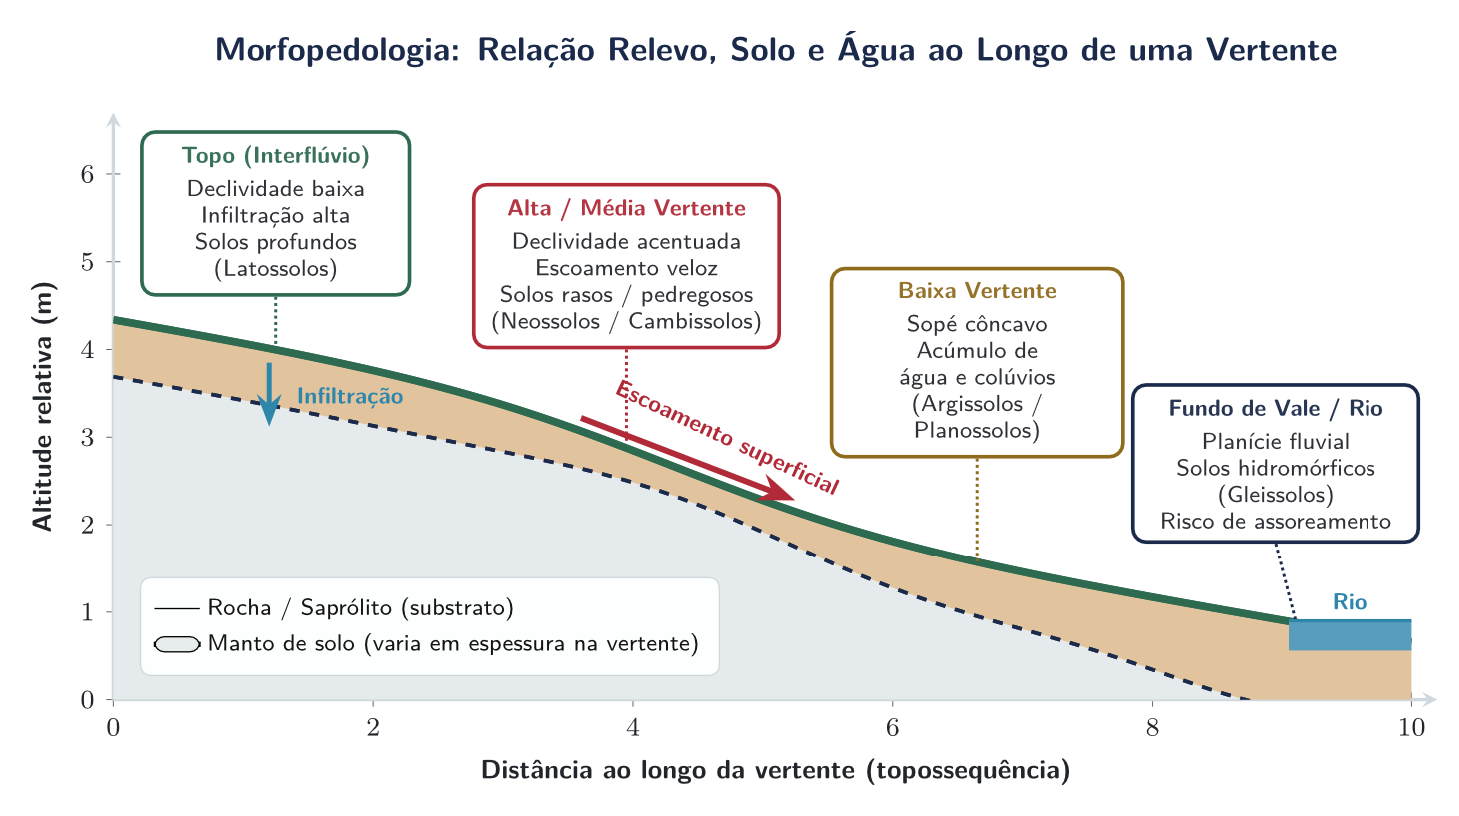
\includegraphics[keepaspectratio]{capitulos/../img/fig06_morfopedologia_vertente.png}}

}

\caption{\label{fig-morfopedologia_vertente}Perfil morfopedológico
integrado de uma vertente (topossequência), evidenciando a variação da
espessura do manto de solo, do balanço infiltração/escoamento e das
classes pedológicas do topo ao fundo de vale.}

\end{figure}%

\begin{longtable}[]{@{}
  >{\raggedright\arraybackslash}p{(\linewidth - 8\tabcolsep) * \real{0.2000}}
  >{\raggedright\arraybackslash}p{(\linewidth - 8\tabcolsep) * \real{0.2000}}
  >{\raggedright\arraybackslash}p{(\linewidth - 8\tabcolsep) * \real{0.2000}}
  >{\raggedright\arraybackslash}p{(\linewidth - 8\tabcolsep) * \real{0.2000}}
  >{\raggedright\arraybackslash}p{(\linewidth - 8\tabcolsep) * \real{0.2000}}@{}}
\caption{Relação genética entre setores da vertente, dinâmica hídrica,
classes de solos e susceptibilidade
ambiental.}\label{tbl-topossequencia}\tabularnewline
\toprule\noalign{}
\begin{minipage}[b]{\linewidth}\raggedright
\textbf{Setor da Vertente}
\end{minipage} & \begin{minipage}[b]{\linewidth}\raggedright
\textbf{Forma / Declividade}
\end{minipage} & \begin{minipage}[b]{\linewidth}\raggedright
\textbf{Dinâmica Hídrica Dominante}
\end{minipage} & \begin{minipage}[b]{\linewidth}\raggedright
\textbf{Solos Típicos (SiBCS)}
\end{minipage} & \begin{minipage}[b]{\linewidth}\raggedright
\textbf{Fragilidade / Processo Principal}
\end{minipage} \\
\midrule\noalign{}
\endfirsthead
\toprule\noalign{}
\begin{minipage}[b]{\linewidth}\raggedright
\textbf{Setor da Vertente}
\end{minipage} & \begin{minipage}[b]{\linewidth}\raggedright
\textbf{Forma / Declividade}
\end{minipage} & \begin{minipage}[b]{\linewidth}\raggedright
\textbf{Dinâmica Hídrica Dominante}
\end{minipage} & \begin{minipage}[b]{\linewidth}\raggedright
\textbf{Solos Típicos (SiBCS)}
\end{minipage} & \begin{minipage}[b]{\linewidth}\raggedright
\textbf{Fragilidade / Processo Principal}
\end{minipage} \\
\midrule\noalign{}
\endhead
\bottomrule\noalign{}
\endlastfoot
Topo (interflúvio) & Plano a suave (\(< 8\%\)) & Infiltração vertical
intensa & Latossolos (profundos) & Baixa erosão natural; sensível à
compactação agrícola. \\
Ombro (alta vertente) & Convexo (\(8\text{-}20\%\)) & Aceleração do
escoamento difuso & Latossolos / Argissolos & Erosão laminar e início de
sulcos em solo exposto. \\
Meia encosta & Retilíneo íngreme (\(> 20\%\)) & Escoamento veloz e
remoção ativa & Neossolos Litólicos e Cambissolos & Alta fragilidade,
ravinas e movimentos de massa. \\
Sopé (baixa vertente) & Côncavo (\(3\text{-}12\%\)) & Convergência de
fluxos e coluvionamento & Argissolos e Planossolos & Erosão em
ravinas/voçorocas por fluxo subsuperficial. \\
Fundo de vale & Plano (\(< 3\%\)) & Saturação hídrica e inundação &
Gleissolos e Neossolos Flúvicos & Assoreamento do canal e inundações
sazonais. \\
\end{longtable}

\subsection{Declividade da Vertente, Cálculo e Classificação (EMBRAPA e
Ross)}\label{declividade-da-vertente-cuxe1lculo-e-classificauxe7uxe3o-embrapa-e-ross}

A \textbf{declividade} é o principal parâmetro quantitativo que expressa
a energia gravitacional atuante sobre uma encosta. Quanto maior a
declividade, maior é a componente tangencial da gravidade que acelera o
escoamento superficial e solicita o solo ao cisalhamento (deslizamento).
Na Geografia e na Engenharia Ambiental, a declividade é expressa de duas
maneiras complementares, em \textbf{porcentagem (\(S\%\))} e em
\textbf{graus (\(\theta\))}.

\subsection{\texorpdfstring{Declividade de Vertentes em Porcentagem
(\(S\%\)) e em Graus
(\(\theta\))}{Declividade de Vertentes em Porcentagem (S\textbackslash\%) e em Graus (\textbackslash theta)}}\label{declividade-de-vertentes-em-porcentagem-s-e-em-graus-theta}

\textbf{Origem e finalidade.} Derivada da trigonometria do triângulo
retângulo formado pela projeção horizontal e pelo desnível vertical do
terreno, a declividade quantifica o grau de inclinação de uma rampa para
fins de mapeamento pedológico (EMBRAPA), análise de fragilidade
ambiental (Ross, 1994), planejamento urbano e aplicação do Código
Florestal (encostas com \(\theta > 45^\circ\), ou \(S > 100\%\), são
APPs).

\textbf{Equações fundamentais,}

\[
S(\%) = \frac{\Delta h}{d_h} \times 100 \qquad\text{e}\qquad \theta = \arctan\!\left(\frac{\Delta h}{d_h}\right)
\]

\textbf{Relações auxiliares indispensáveis em Geografia,}

\textbf{A partir de carta topográfica (escala \(1:E\)).} Se a distância
medida no mapa entre duas curvas de nível é \(d_{\text{mapa}}\) (em
metros ou convertida de cm para m), então
\(d_h = d_{\text{mapa}} \times E\). \textbf{A partir de trena no terreno
(distância inclinada \(d_{\text{inc}}\)).} Pelo Teorema de Pitágoras,
obtém-se primeiro a distância horizontal,

\[
d_h = \sqrt{d_{\text{inc}}^2 - \Delta h^2}.
\]

. \textbf{Conversão direta entre graus e porcentagem,}
\(S(\%) = 100 \cdot \tan\theta\) e \(\theta = \arctan(S / 100)\).

\textbf{Variáveis e unidades,} \(\Delta h\) e \(d_h\) devem estar
obrigatoriamente na \textbf{mesma unidade de comprimento} (ambos em
metros, por exemplo).

\textbf{Exemplo numérico completo.} Uma encosta desce da cota
\(316\text{ m}\) para a cota \(280\text{ m}\) ao longo de uma distância
horizontal de \(d_h = 200\text{ m}\).

\[
\begin{aligned}
\Delta h &= 316 - 280 = 36\text{ m} \\
S(\%) &= \frac{36}{200} \times 100 = 0{,}18 \times 100 = 18{,}0\% \\
\theta &= \arctan(0{,}18) \approx 10{,}20^\circ.
\end{aligned}
\]

\textbf{Interpretação.} A cada \(100\text{ m}\) percorridos na
horizontal, o terreno sobe ou desce \(18\text{ m}\). Pelas classes da
Tabela~\hyperref[tbl-classes_declividade]{classes declividade}, o relevo
é \textbf{Ondulado} (EMBRAPA) e apresenta \textbf{Fragilidade Média,
Classe 3} (Ross, 1994).

Note um marco conceitual que elimina erros em provas, \textbf{uma
declividade de \(45^\circ\) corresponde exatamente a \(100\%\)}, pois
\(\tan(45^\circ) = 1\), o que significa que \(\Delta h = d_h\) (o
terreno sobe \(1\text{ m}\) a cada \(1\text{ m}\) na horizontal).
Consequentemente, rampas mais íngremes que \(45^\circ\) possuem
declividades \textbf{superiores a \(100\%\)} (por exemplo, \(60^\circ\)
equivale a \(\tan(60^\circ) \times 100 \approx 173,2\%\)).

{\def\LTcaptype{none} % do not increment counter
\begin{longtable}[]{@{}
  >{\raggedright\arraybackslash}p{(\linewidth - 4\tabcolsep) * \real{0.3333}}
  >{\raggedright\arraybackslash}p{(\linewidth - 4\tabcolsep) * \real{0.3333}}
  >{\raggedright\arraybackslash}p{(\linewidth - 4\tabcolsep) * \real{0.3333}}@{}}
\toprule\noalign{}
\begin{minipage}[b]{\linewidth}\raggedright
Declividade em porcentagem
\end{minipage} & \begin{minipage}[b]{\linewidth}\raggedright
Ângulo aproximado
\end{minipage} & \begin{minipage}[b]{\linewidth}\raggedright
Classe de relevo da Embrapa
\end{minipage} \\
\midrule\noalign{}
\endhead
\bottomrule\noalign{}
\endlastfoot
De 0 a 3\% & De 0° a 1,7° & Plano. \\
De 3 a 8\% & De 1,7° a 4,6° & Suave ondulado. \\
De 8 a 20\% & De 4,6° a 11,3° & Ondulado. \\
De 20 a 45\% & De 11,3° a 24,2° & Forte ondulado. \\
De 45 a 75\% & De 24,2° a 36,9° & Montanhoso. \\
Maior que 75\% & Maior que 36,9° & Escarpado. \\
\end{longtable}
}

A classificação de relevo da Embrapa e as classes de fragilidade de Ross
utilizam limites diferentes. Por essa razão, a mesma linha da primeira
classificação pode abranger mais de uma classe da segunda. A comparação
deve utilizar a declividade medida, mantendo separados os dois
critérios.

\begin{longtable}[]{@{}
  >{\raggedright\arraybackslash}p{(\linewidth - 2\tabcolsep) * \real{0.5000}}
  >{\raggedright\arraybackslash}p{(\linewidth - 2\tabcolsep) * \real{0.5000}}@{}}
\caption{Classes de declividade segundo a EMBRAPA (relevo pedológico) e
segundo Ross (1994) (fragilidade do relevo), com correspondência
aproximada em graus e implicações
ambientais.}\label{tbl-classes_declividade}\tabularnewline
\toprule\noalign{}
\begin{minipage}[b]{\linewidth}\raggedright
Declividade de referência
\end{minipage} & \begin{minipage}[b]{\linewidth}\raggedright
Classe de fragilidade do relevo segundo Ross
\end{minipage} \\
\midrule\noalign{}
\endfirsthead
\toprule\noalign{}
\begin{minipage}[b]{\linewidth}\raggedright
Declividade de referência
\end{minipage} & \begin{minipage}[b]{\linewidth}\raggedright
Classe de fragilidade do relevo segundo Ross
\end{minipage} \\
\midrule\noalign{}
\endhead
\bottomrule\noalign{}
\endlastfoot
Menor que 6\% & 1, muito fraca. \\
De 6\% a menos de 12\% & 2, fraca. \\
De 12\% a menos de 20\% & 3, média. \\
De 20\% até 30\% & 4, forte. \\
Acima de 30\% & 5, muito forte. \\
\end{longtable}

\subsection{Cobertura Vegetal, Erosão em Vertentes e Movimentos de
Massa}\label{cobertura-vegetal-erosuxe3o-em-vertentes-e-movimentos-de-massa}

\subsubsection{Papel da Cobertura Vegetal no Balanço Infiltração
vs.~Escoamento}\label{papel-da-cobertura-vegetal-no-balanuxe7o-infiltrauxe7uxe3o-vs.-escoamento}

A cobertura vegetal constitui a primeira linha de defesa da vertente
contra a degradação. Sua atuação ocorre em três níveis integrados,

\textbf{Dossel aéreo (copas e estratos arbustivos).} Intercepta parte da
chuva (retornando-a à atmosfera por evaporação) e quebra a energia
cinética das gotas antes que atinjam o solo, impedindo o efeito
\textbf{splash} (salpicamento) que desagrega torrões e cria crostas de
selamento superficial. \textbf{Serapilheira (folhedo sobre o solo).}
Funciona como manta protetora de alta rugosidade hidráulica, reduzindo a
velocidade do escoamento superficial e ampliando o tempo disponível para
a água penetrar no solo.

\textbf{Sistema radicular e atividade biológica.} Raízes e fauna edáfica
formam canais contínuos (\textbf{macroporosidade}) que elevam
drasticamente a taxa de infiltração; simultaneamente, a
evapotranspiração retira excesso de água do perfil (reduzindo a
poropressão positiva) e as raízes acrescentam resistência mecânica ao
cisalhamento (coesão radicular, tema aprofundado no Cap. 13).

Quando essa proteção é removida, o escoamento superficial concentrado
evolui progressivamente de erosão laminar para sulcos, ravinas e
voçorocas (detalhados no Cap. 12), exportando grandes volumes de solo
para o sopé e para os canais fluviais, onde geram \textbf{assoreamento},
caracterizado pela redução da profundidade da calha, pela perda de
capacidade de armazenamento de açudes e pela ampliação das manchas de
inundação.

\subsubsection{Movimentos de Massa em
Encostas}\label{movimentos-de-massa-em-encostas}

Enquanto a erosão hídrica transporta partículas de solo gradualmente
pela ação da água corrente, os \textbf{movimentos de massa} (ou
movimentos gravitacionais de massa) consistem no deslocamento coletivo
de volumes expressivos de solo, saprólito e/ou rocha encosta abaixo,
impulsionados diretamente pela força da gravidade quando as tensões
cisalhantes superam a resistência interna do material (Guerra, 2018;
Varnes, 1978).

Na análise ambiental e na gestão de riscos em encostas, processos
frequentes em áreas serranas e em bairros periféricos sobre relevo
acidentado na Bahia (como Salvador, cidades do Recôncavo e bordas de
serras), distinguem-se cinco tipos principais, sistematizados na
Tabela~\hyperref[tbl-movimentos_massa]{movimentos massa}.

\begin{longtable}[]{@{}
  >{\raggedright\arraybackslash}p{(\linewidth - 8\tabcolsep) * \real{0.2000}}
  >{\raggedright\arraybackslash}p{(\linewidth - 8\tabcolsep) * \real{0.2000}}
  >{\raggedright\arraybackslash}p{(\linewidth - 8\tabcolsep) * \real{0.2000}}
  >{\raggedright\arraybackslash}p{(\linewidth - 8\tabcolsep) * \real{0.2000}}
  >{\raggedright\arraybackslash}p{(\linewidth - 8\tabcolsep) * \real{0.2000}}@{}}
\caption{Quadro comparativo dos principais tipos de movimentos de massa
em encostas.}\label{tbl-movimentos_massa}\tabularnewline
\toprule\noalign{}
\begin{minipage}[b]{\linewidth}\raggedright
\textbf{Tipo de Movimento}
\end{minipage} & \begin{minipage}[b]{\linewidth}\raggedright
\textbf{Velocidade}
\end{minipage} & \begin{minipage}[b]{\linewidth}\raggedright
\textbf{Geometria / Mecanismo}
\end{minipage} & \begin{minipage}[b]{\linewidth}\raggedright
\textbf{Principais Gatilhos}
\end{minipage} & \begin{minipage}[b]{\linewidth}\raggedright
\textbf{Feições Diagnósticas em Campo}
\end{minipage} \\
\midrule\noalign{}
\endfirsthead
\toprule\noalign{}
\begin{minipage}[b]{\linewidth}\raggedright
\textbf{Tipo de Movimento}
\end{minipage} & \begin{minipage}[b]{\linewidth}\raggedright
\textbf{Velocidade}
\end{minipage} & \begin{minipage}[b]{\linewidth}\raggedright
\textbf{Geometria / Mecanismo}
\end{minipage} & \begin{minipage}[b]{\linewidth}\raggedright
\textbf{Principais Gatilhos}
\end{minipage} & \begin{minipage}[b]{\linewidth}\raggedright
\textbf{Feições Diagnósticas em Campo}
\end{minipage} \\
\midrule\noalign{}
\endhead
\bottomrule\noalign{}
\endlastfoot
\textbf{Rastejo (\emph{creep})} & Muito lenta (\(\text{mm}\) a
\(\text{cm}/\text{ano}\)) & Deformação plástica contínua sem plano
nítido de ruptura & Ciclos de umedecimento/secagem e gravidade contínua
& Árvores com troncos encurvados na base, cercas e postes inclinados,
trincas lentas em muros. \\
\textbf{Escorregamento rotacional} & Moderada a rápida (\(\text{m/h}\) a
\(\text{m/s}\)) & Superfície de ruptura curva (côncava em forma de
colher) & Chuvas prolongadas, elevação da poropressão, cortes no pé do
talude & Cicatriz em arco no topo, degrau de abatimento, massa tombada
para trás e lóbulo no pé. \\
\textbf{Escorregamento translacional (planar)} & Rápida a muito rápida
(\(\text{m/s}\)) & Superfície de ruptura plana (contato solo-rocha ou
fratura) & Chuvas intensas rápidas em solos rasos de encostas íngremes &
Cicatriz rasa e alongada expondo rocha/saprólito; material desliza como
placa extensa. \\
\textbf{Corrida de lama / detritos} & Muito rápida a extremamente rápida
& Fluxo viscoso saturado comportando-se como fluido denso & Chuvas
extremas canalizadas em vales íngremes com solo solto & Canais escavados
em U, blocos arrastados a longas distâncias e leques espessos no
sopé. \\
\textbf{Queda de blocos} & Extremamente rápida (queda livre) &
Desprendimento abrupto de blocos em paredões subverticais & Fraturamento
rochoso, alívio de tensão, raízes em fendas, chuvas & Acúmulo de blocos
angulosos (depósito de tálus) na base de escarpas e falésias. \\
\end{longtable}

\subsection{Fatores Naturais vs.~Antrópicos na Fragilidade de
Encostas}\label{fatores-naturais-vs.-antruxf3picos-na-fragilidade-de-encostas}

A instabilidade de uma vertente resulta da interação entre
\textbf{fatores condicionantes} (declividade elevada, solos rasos sobre
rocha impermeável, fraturas inclinadas a favor do talude) e
\textbf{fatores deflagradores} (chuvas intensas ou prolongadas). A
ocupação humana desordenada agrava criticamente ambos os lados dessa
equação ao, (1) executar \textbf{cortes verticais no pé da encosta}
(removendo o apoio lateral natural); (2) lançar \textbf{aterros mal
compactados e lixo} no topo (aumentando o peso solicitante); (3)
infiltrar \textbf{águas servidas e fossas} diretamente no talude
(elevando a poropressão mesmo fora do período chuvoso); e (4) suprimir a
cobertura vegetal arbórea.

\subsection{Circulação da água e descontinuidades na
vertente}\label{circulauxe7uxe3o-da-uxe1gua-e-descontinuidades-na-vertente}

A água que infiltra encontra camadas com condutividade hidráulica
distinta. Um horizonte mais restritivo pode favorecer armazenamento
temporário e fluxo lateral sobre seu limite. Em uma encosta, esse fluxo
pode reaparecer como surgência, especialmente quando o relevo intercepta
a camada saturada.

A interpretação exige descrever a posição de cada perfil e a
continuidade dos horizontes. Cor, estrutura, espessura, raízes e sinais
de redução do ferro ajudam a reconhecer condições de drenagem. A
presença de uma cor isolada deve ser interpretada junto ao material de
origem e à organização do perfil, evitando conclusões a partir de um
único atributo.

Uma estrada pode interceptar o fluxo lateral e redistribuí-lo por
valetas e bueiros. A concentração em uma saída sem proteção aumenta a
descarga localizada sobre a vertente. A erosão observada a jusante passa
a depender da área efetivamente drenada pela estrada, que pode diferir
da contribuição topográfica original.

O planejamento morfopedológico relaciona essas observações às
intervenções. Conservação da cobertura, distribuição de descargas e
proteção das saídas de drenagem precisam responder ao percurso da água.
O desenho final deve ser conferido em campo após eventos de chuva,
quando caminhos preferenciais e pontos de exfiltração ficam mais
evidentes.

\section{Etapa 4 - Exemplos
resolvidos}\label{etapa-4---exemplos-resolvidos-7}

\subsection{Exemplo 8.1 - Declividade e Solos ao Longo de uma
Topossequência (Nível
Básico)}\label{exemplo-8.1---declividade-e-solos-ao-longo-de-uma-topossequuxeancia-nuxedvel-buxe1sico}

\textbf{Situação analisada.} Durante um trabalho de campo da disciplina
CHF662, os estudantes levantaram três segmentos consecutivos de uma
mesma vertente, o \textbf{Topo} (desnível de \(6\text{ m}\) em
\(300\text{ m}\) horizontais), a \textbf{Meia Encosta} (desnível de
\(54\text{ m}\) em \(150\text{ m}\) horizontais) e o \textbf{Sopé}
(desnível de \(12\text{ m}\) em \(200\text{ m}\) horizontais).

\textbf{Dados disponíveis.} Topo,
\(\Delta h = 6\text{ m}, d_h = 300\text{ m}\). Meia Encosta,
\(\Delta h = 54\text{ m}, d_h = 150\text{ m}\). Sopé,
\(\Delta h = 12\text{ m}, d_h = 200\text{ m}\).

\textbf{Problema a resolver.} Calcular a declividade em porcentagem
(\(S\%\)) e em graus (\(\theta\)) de cada setor, classificá-los segundo
EMBRAPA e Ross (1994) e indicar o solo esperado em cada posição da
topossequência.

\textbf{Fundamento da análise.} Aplicação de
\(S(\%) = (\Delta h / d_h)\times 100\) e
\(\theta = \arctan(\Delta h / d_h)\), com enquadramento pelas
Tabelas~\hyperref[tbl-topossequencia]{topossequencia}
e~\hyperref[tbl-classes_declividade]{classes declividade}.

\textbf{Desenvolvimento.}

\textbf{Topo,}

\[
S_1 = \frac{6}{300} \times 100 = 0{,}02 \times 100 = 2{,}0\% \qquad;\qquad \theta_1 = \arctan(0{,}02) \approx 1{,}15^\circ.
\]

. \textbf{Meia Encosta,}

\[
S_2 = \frac{54}{150} \times 100 = 0{,}36 \times 100 = 36{,}0\% \qquad;\qquad \theta_2 = \arctan(0{,}36) \approx 19{,}80^\circ.
\]

. \textbf{Sopé,}

\[
S_3 = \frac{12}{200} \times 100 = 0{,}06 \times 100 = 6{,}0\% \qquad;\qquad \theta_3 = \arctan(0{,}06) \approx 3{,}43^\circ.
\]

.

\textbf{Interpretação do resultado.} Topo, \(2,0\%\) (\(1,15^\circ\)),
EMBRAPA Plano / Ross Classe 1 (Muito Fraca), com predomínio de
\textbf{Latossolos}. Meia Encosta, \(36,0\%\) (\(19,80^\circ\)), EMBRAPA
Forte ondulado / Ross Classe 5 (Muito Forte, \(>30\%\)), com
\textbf{Neossolos Litólicos / Cambissolos}. Sopé, \(6,0\%\)
(\(3,43^\circ\)), EMBRAPA Suave ondulado / Ross Classe 2 (Fraca,
\(6\text{-}12\%\)), com \textbf{Argissolos / Planossolos}.

\textbf{Condições de validade.} O perfil numérico reproduz o
comportamento clássico da Figura~\ref{fig-morfopedologia_vertente},
declividade mínima no topo (máxima infiltração e solo profundo), salto
abrupto na meia encosta (predomínio erosivo e solo raso) e suavização no
sopé (acumulação coluvial).

\subsection{Exemplo 8.2 - Cálculo de Declividade a partir de Carta
Topográfica (Nível
Básico-Intermediário)}\label{08-morfopedologia-vertentes-exemplo-8.2.-cuxe1lculo-de-declividade-a-partir-de-carta-topogruxe1fica-nuxedvel-buxe1sicointermediuxe1rio}

\textbf{Situação analisada.} Em uma carta topográfica na escala
\textbf{1,25.000}, duas curvas de nível de cotas \(260\text{ m}\) e
\(320\text{ m}\) estão separadas, em linha reta perpendicular às curvas,
por uma distância medida na régua de
\(d_{\text{mapa}} = 1,2\text{ cm}\).

\textbf{Dados disponíveis.} Escala \(1:25.000\) (\(E = 25.000\));
\(H_1 = 260\text{ m}\); \(H_2 = 320\text{ m}\);
\(d_{\text{mapa}} = 1,2\text{ cm}\).

\textbf{Problema a resolver.} Determinar a distância horizontal real
(\(d_h\)), o desnível (\(\Delta h\)), a declividade em porcentagem
(\(S\%\)) e em graus (\(\theta\)), e sua classe segundo EMBRAPA e Ross.

\textbf{Fundamento da análise.} Conversão da distância cartográfica para
distância horizontal real em metros
(\(d_h = d_{\text{mapa}} \times E\)), seguida do cálculo de \(S(\%)\) e
\(\theta\).

\textbf{Desenvolvimento.}

\textbf{Distância horizontal real (\(d_h\)),}

\[
d_h = 1{,}2\text{ cm} \times 25.000 = 30.000\text{ cm}.
\]

Convertendo centímetros para metros (dividindo por \(100\)),

\[
d_h = \frac{30.000}{100} = 300\text{ m}.
\]

. \textbf{Desnível vertical (\(\Delta h\)),}

\[
\Delta h = 320 - 260 = 60\text{ m}.
\]

. \textbf{Declividade em porcentagem e em graus,}

\[
S(\%) = \frac{60}{300} \times 100 = 0{,}20 \times 100 = 20{,}0\% \qquad;\qquad \theta = \arctan(0{,}20) \approx 11{,}31^\circ.
\]

.

\textbf{Interpretação do resultado.} \(d_h = 300\text{ m}\),
\(\Delta h = 60\text{ m}\), \(S = 20,0\%\) e
\(\theta \approx 11,31^\circ\). Classe EMBRAPA, limite superior de
Ondulado (\(8\text{-}20\%\)); Classe Ross, início da Classe 4, Forte
(\(20\text{-}30\%\)).

\textbf{Condições de validade.} Em escala 1,25.000, cada \(1\text{ cm}\)
vale \(250\text{ m}\); logo \(1,2\text{ cm}\) corresponde a
\(250 + 50 = 300\text{ m}\), confirmando a conversão. Como
\(60 / 300 = 1/5 = 0,20\), a declividade de \(20\%\) e o ângulo de
\(11,31^\circ\) são exatos e alertam para a necessidade de práticas
conservacionistas rigorosas.

\subsection{Exemplo 8.3 - Correção de Distância Inclinada Medida com
Trena em Campo (Nível
Intermediário)}\label{exemplo-8.3---correuxe7uxe3o-de-distuxe2ncia-inclinada-medida-com-trena-em-campo-nuxedvel-intermediuxe1rio}

\textbf{Situação analisada.} Durante uma vistoria de encosta sem mapa
detalhado, um técnico mediu com trena apoiada sobre a superfície do
terreno uma rampa de comprimento inclinado
\(d_{\text{inc}} = 100\text{ m}\). Com auxílio de nível
topográfico/altímetro de precisão, verificou-se um desnível vertical de
\(\Delta h = 28\text{ m}\) entre a base e o topo dessa rampa.

\textbf{Dados disponíveis.} \(d_{\text{inc}} = 100\text{ m}\);
\(\Delta h = 28\text{ m}\).

\textbf{Problema a resolver.} Calcular a distância horizontal real
(\(d_h\)), a declividade correta (\(S\%\) e \(\theta\)) e mostrar qual
seria o erro caso o técnico utilizasse indevidamente \(d_{\text{inc}}\)
no lugar de \(d_h\).

\textbf{Fundamento da análise.} Aplicação do Teorema de Pitágoras
(\(d_h = \sqrt{d_{\text{inc}}^2 - \Delta h^2}\)) antes de calcular
\(S(\%) = (\Delta h / d_h)\times 100\) e
\(\theta = \arctan(\Delta h / d_h)\).

\textbf{Desenvolvimento.}

\textbf{Cálculo da distância horizontal (\(d_h\)),}

\[
d_h = \sqrt{100^2 - 28^2} = \sqrt{10.000 - 784} = \sqrt{9.216} = 96{,}0\text{ m}.
\]

. \textbf{Declividade correta em porcentagem e graus,}

\[
S(\%) = \frac{28}{96} \times 100 \approx 0{,}2917 \times 100 = 29{,}17\% \qquad;\qquad \theta = \arctan\!\left(\frac{28}{96}\right) \approx 16{,}26^\circ.
\]

. \textbf{Comparação com o erro de usar \(d_{\text{inc}}\) diretamente.}
Se o técnico dividisse \(28 / 100\), obteria \(28,00\%\) (subestimando a
declividade em \(1,17\) ponto percentual, pois \(28/100 = \sin\theta\) e
não \(\tan\theta\)).

\textbf{Interpretação do resultado.} \(d_h = 96,0\text{ m}\);
declividade correta \(S = 29,17\%\) e \(\theta \approx 16,26^\circ\)
(EMBRAPA, Forte ondulado; Ross, Classe 4, Forte, quase no limite da
Classe 5).

\textbf{Condições de validade.} Como a hipotenusa
(\(d_{\text{inc}} = 100\text{ m}\)) é sempre maior que o cateto
horizontal (\(d_h = 96\text{ m}\)), usar a distância medida pela trena
no denominador sempre subestima a declividade real, erro que se torna
muito grave em encostas acima de \(30\%\).

\subsection{Exemplo 8.4 - Efeito da Cobertura Vegetal no Balanço
Infiltração vs.~Escoamento (Nível
Intermediário)}\label{exemplo-8.4---efeito-da-cobertura-vegetal-no-balanuxe7o-infiltrauxe7uxe3o-vs.-escoamento-nuxedvel-intermediuxe1rio}

\textbf{Situação analisada.} Duas parcelas experimentais adjacentes em
uma mesma meia encosta (\(S = 18\%\)) receberam uma chuva de
\(80\text{ mm}\), a \textbf{Parcela 1} possui cobertura de Caatinga
arbóreo-arbustiva conservada com serapilheira (infiltração/retenção de
\(85\%\) e escoamento superficial de \(15\%\)); a \textbf{Parcela 2}
encontra-se com solo exposto após queimada e pisoteio bovino
(infiltração de \(25\%\) e escoamento superficial de \(75\%\)).

\textbf{Dados disponíveis.} Chuva total \(P = 80\text{ mm}\). Parcela 1,
\(85\%\) infiltração, \(15\%\) escoamento. Parcela 2, \(25\%\)
infiltração, \(75\%\) escoamento.

\textbf{Problema a resolver.} Calcular as lâminas infiltradas e escoadas
(em \(\text{mm}\) e em litros por \(\text{m}^2\)) em cada parcela, a
razão entre os escoamentos e os reflexos morfopedológicos esperados.

\textbf{Fundamento da análise.} Cálculo proporcional das lâminas
(\(L_{\text{inf}}\) e \(L_{\text{esc}}\)) usando a equivalência
\(1\text{ mm} = 1\text{ L/m}^2\).

\textbf{Desenvolvimento.}

\textbf{Parcela 1 (vegetação conservada),}

\[
\begin{aligned}
L_{\text{inf},1} &= 0{,}85 \times 80\text{ mm} = 68{,}0\text{ mm} \;\; (68\text{ L/m}^2) \\
L_{\text{esc},1} &= 0{,}15 \times 80\text{ mm} = 12{,}0\text{ mm} \;\; (12\text{ L/m}^2).
\end{aligned}
\]

. \textbf{Parcela 2 (solo exposto),}

\[
\begin{aligned}
L_{\text{inf},2} &= 0{,}25 \times 80\text{ mm} = 20{,}0\text{ mm} \;\; (20\text{ L/m}^2) \\
L_{\text{esc},2} &= 0{,}75 \times 80\text{ mm} = 60{,}0\text{ mm} \;\; (60\text{ L/m}^2).
\end{aligned}
\]

. \textbf{Comparação do escoamento superficial,}

\[
\frac{L_{\text{esc},2}}{L_{\text{esc},1}} = \frac{60{,}0}{12{,}0} = 5{,}0\text{ vezes}.
\]

.

\textbf{Interpretação do resultado.} Na parcela conservada infiltram
\(68\text{ L/m}^2\) e escoam \(12\text{ L/m}^2\); no solo exposto
infiltram apenas \(20\text{ L/m}^2\) e escoam \(60\text{ L/m}^2\), um
volume superficial \(5\) vezes maior.

\textbf{Condições de validade.} Observe a soma em ambas as parcelas
(\(68 + 12 = 80\text{ mm}\); \(20 + 60 = 80\text{ mm}\)). Sobre uma
vertente de \(18\%\), multiplicar o escoamento por cinco sem a
rugosidade da serapilheira desencadeia rapidamente erosão laminar,
sulcos e assoreamento do sopé, além de reduzir em \(70,6\%\) a água
disponível para recarga e sobrevivência da vegetação na estação seca.

\subsection{Exemplo 8.5 - Instabilização de Encosta Urbana por Corte de
Talude (Nível
Avançado)}\label{exemplo-8.5---instabilizauxe7uxe3o-de-encosta-urbana-por-corte-de-talude-nuxedvel-avanuxe7ado}

\textbf{Situação analisada.} Uma encosta natural com solo argilo-arenoso
espesso apresenta desnível \(\Delta h = 27\text{ m}\) distribuído ao
longo de uma distância horizontal \(d_{h1} = 150\text{ m}\). Para
implantar um conjunto de residências sem projeto geotécnico, executou-se
um corte no sopé da vertente, concentrando o mesmo desnível de
\(27\text{ m}\) em uma distância horizontal reduzida para
\(d_{h2} = 45\text{ m}\), acompanhado de lançamento de águas servidas a
montante.

\textbf{Dados disponíveis.} \(\Delta h = 27\text{ m}\); cenário natural
\(d_{h1} = 150\text{ m}\); cenário após corte \(d_{h2} = 45\text{ m}\).

\textbf{Problema a resolver.} Calcular a declividade (\(S\%\) e
\(\theta\)) antes e depois da intervenção, verificar se ultrapassa o
limite de APP de \(45^\circ\) (\(100\%\)), identificar o tipo de
movimento de massa mais provável e justificar os mecanismos envolvidos.

\textbf{Fundamento da análise.} Cálculo comparativo de \(S(\%)\) e
\(\theta\) e diagnóstico geotécnico-morfopedológico baseado na
Tabela~\hyperref[tbl-movimentos_massa]{movimentos massa}.

\textbf{Desenvolvimento.}

\textbf{Encosta natural (\(d_{h1} = 150\text{ m}\)),}

\[
S_1 = \frac{27}{150} \times 100 = 18{,}0\% \qquad;\qquad \theta_1 = \arctan(0{,}18) \approx 10{,}20^\circ.
\]

. \textbf{Talude após corte (\(d_{h2} = 45\text{ m}\)),}

\[
S_2 = \frac{27}{45} \times 100 = 60{,}0\% \qquad;\qquad \theta_2 = \arctan(0{,}60) \approx 30{,}96^\circ.
\]

. \textbf{Verificação do limite legal de \(45^\circ\) (\(100\%\)).} Como
\(30,96^\circ < 45^\circ\) (\(60\% < 100\%\)), o talude não atingiu o
patamar de APP de encosta (\(>45^\circ\)), mas saltou da Classe 3 de
Ross (Média) para a \textbf{Classe 5 (Muito Forte, \(>30\%\))} e da
classe Ondulado para \textbf{Montanhoso (EMBRAPA)}.

\textbf{Interpretação do resultado.} A declividade mais que triplicou,
passando de \(18,0\%\) (\(10,20^\circ\)) para \(60,0\%\)
(\(30,96^\circ\)). Em solo argilo-arenoso espesso sujeito a corte no pé
e saturação por águas servidas, o movimento de massa mais provável é o
\textbf{escorregamento rotacional}.

\textbf{Condições de validade.} O resultado demonstra um ponto crucial
de Análise Ambiental, uma encosta não precisa atingir \(45^\circ\)
(\(100\%\)) para apresentar risco crítico! O corte retira o contraforte
natural na base do maciço de solo, enquanto as águas servidas elevam a
poropressão e reduzem o atrito interno, criando condições clássicas para
ruptura curva (rotacional) durante eventos de chuva prolongada.

\section{Etapa 5 - Erros de
interpretação}\label{etapa-5---erros-de-interpretauxe7uxe3o-7}

\subsection{\texorpdfstring{Erro 1, Achar que \(100\%\) de declividade
equivale a um paredão vertical de
\(90^\circ\)}{Erro 1, Achar que 100\textbackslash\% de declividade equivale a um paredão vertical de 90\^{}\textbackslash circ}}\label{erro-1-achar-que-100-de-declividade-equivale-a-um-pareduxe3o-vertical-de-90circ}

\textbf{Equívoco frequente.} Associar intuitivamente \(100\%\) ao ângulo
reto (\(90^\circ\)) e concluir que \(45^\circ\) valeria \(50\%\).

\textbf{Correção técnica.} A declividade em porcentagem é
\(100 \times \tan\theta\). Como \(\tan(45^\circ) = 1\), uma encosta de
\textbf{\(45^\circ\) tem exatamente \(100\%\) de declividade}
(\(\Delta h = d_h\)). Já uma parede vertical (\(90^\circ\)) possui
\(d_h = 0\), tendendo a declividade ao infinito.

\subsection{\texorpdfstring{Erro 2, Usar a distância inclinada da trena
no denominador de
\(S(\%)\)}{Erro 2, Usar a distância inclinada da trena no denominador de S(\textbackslash\%)}}\label{erro-2-usar-a-distuxe2ncia-inclinada-da-trena-no-denominador-de-s}

\textbf{Equívoco frequente.} Medir \(50\text{ m}\) inclinados no terreno
com trena e dividir \(\Delta h\) diretamente por \(50\text{ m}\).

\textbf{Correção técnica.} A definição matemática de declividade usa a
\textbf{distância horizontal (\(d_h\))} no denominador
(\(\Delta h / d_h = \tan\theta\)). Quando se dispõe apenas da distância
inclinada (\(d_{\text{inc}}\)), deve-se calcular
\(d_h = \sqrt{d_{\text{inc}}^2 - \Delta h^2}\) antes de aplicar a
fórmula.

\subsection{Erro 3, Confundir escorregamento rotacional com
translacional}\label{erro-3-confundir-escorregamento-rotacional-com-translacional}

\textbf{Equívoco frequente.} Chamar qualquer deslizamento de terra
genericamente de ``desmoronamento'' ou trocar os condicionantes de cada
tipo.

\textbf{Correção técnica.} O \textbf{escorregamento rotacional} ocorre
tipicamente em solos espessos e homogêneos, formando superfície de
ruptura curva (em colher); o \textbf{escorregamento translacional
(planar)} ocorre em solos rasos sobre substrato rochoso ou planos de
fraqueza, deslizando como uma placa paralela à superfície da encosta.

\subsection{Erro 4, Analisar solo e relevo de forma desarticulada no
diagnóstico}\label{erro-4-analisar-solo-e-relevo-de-forma-desarticulada-no-diagnuxf3stico}

\textbf{Equívoco frequente.} Descrever o solo do topo da vertente (por
exemplo, Latossolo profundo) e generalizar suas propriedades de alta
permeabilidade para toda a encosta, incluindo a meia vertente íngreme e
o fundo de vale.

\textbf{Correção técnica.} Pela abordagem morfopedológica, a variação da
declividade e da curvatura altera profundamente a pedogênese ao longo da
topossequência. Cada compartimento (topo, ombro, meia encosta, sopé e
várzea) exige diagnóstico e manejo específicos.

\section{Etapa 6 - Exercícios de
fixação}\label{etapa-6---exercuxedcios-de-fixauxe7uxe3o-7}

\subsubsection{Nível Básico (Exercícios 1 a
5)}\label{nuxedvel-buxe1sico-exercuxedcios-1-a-5-3}

\begin{enumerate}
\def\labelenumi{\arabic{enumi}.}
\item
  Explique o que é uma \textbf{topossequência} na abordagem
  morfopedológica e descreva por que os solos do topo plano tendem a ser
  mais profundos do que os solos da meia encosta íngreme.
\item
  Uma vertente apresenta desnível vertical \(\Delta h = 15\text{ m}\) em
  uma distância horizontal \(d_h = 250\text{ m}\). Calcule sua
  declividade em porcentagem (\(S\%\)) e em graus (\(\theta\)) e
  classifique-a segundo EMBRAPA e Ross (1994).
\item
  Determine \(S(\%)\) e \(\theta\) para uma encosta com
  \(\Delta h = 45\text{ m}\) e \(d_h = 150\text{ m}\), indicando sua
  classe na EMBRAPA e em Ross (1994).
\item
  Demonstre matematicamente por que uma encosta com
  \(\Delta h = 80\text{ m}\) e \(d_h = 80\text{ m}\) corresponde ao
  limite legal de APP de encosta previsto no Código Florestal
  (\(45^\circ\)).
\item
  Em uma carta topográfica na escala \textbf{1,50.000}, duas curvas de
  nível separadas por um desnível \(\Delta h = 40\text{ m}\) distam
  \(0,8\text{ cm}\) no mapa. Calcule a distância horizontal real
  (\(d_h\)) e a declividade (\(S\%\) e \(\theta\)).
\end{enumerate}

\subsubsection{Nível Intermediário (Exercícios 6 a
10)}\label{nuxedvel-intermediuxe1rio-exercuxedcios-6-a-10-3}

\begin{enumerate}
\def\labelenumi{\arabic{enumi}.}
\setcounter{enumi}{5}
\item
  Em campo, mediu-se com trena sobre a rampa uma distância inclinada
  \(d_{\text{inc}} = 50\text{ m}\) correspondente a um desnível
  \(\Delta h = 14\text{ m}\). Calcule a distância horizontal real
  (\(d_h\)) e a declividade correta em porcentagem e em graus.
\item
  Uma vertente foi dividida em três compartimentos para zoneamento
  agrícola,

  \begin{itemize}
  \item
    \textbf{Setor A (topo),} \(\Delta h = 10\text{ m}\),
    \(d_h = 400\text{ m}\).
  \item
    \textbf{Setor B (meia encosta),} \(\Delta h = 64\text{ m}\),
    \(d_h = 160\text{ m}\).
  \item
    \textbf{Setor C (sopé),} \(\Delta h = 20\text{ m}\),
    \(d_h = 250\text{ m}\).
  \end{itemize}

  Calcule \(S(\%)\) e \(\theta\) de cada setor, classifique-os segundo
  EMBRAPA e Ross e indique o uso mais adequado para cada compartimento.
\item
  Explique como a remoção da cobertura vegetal altera simultaneamente o
  efeito \emph{splash}, a macroporosidade superficial e o risco de
  assoreamento no fundo de vale.
\item
  Diferencie \textbf{rastejo}, \textbf{escorregamento translacional} e
  \textbf{corrida de detritos} quanto à velocidade do deslocamento e às
  feições visíveis em campo.
\item
  Por que a infiltração de águas servidas (esgoto doméstico sem coleta)
  em encostas ocupadas pode deflagrar movimentos de massa mesmo após
  chuvas moderadas? Utilize o conceito de \textbf{poropressão} na sua
  explicação.
\end{enumerate}

\subsubsection{Questões Objetivas (Exercícios 11 a
15)}\label{questuxf5es-objetivas-exercuxedcios-11-a-15-1}

\begin{enumerate}
\def\labelenumi{\arabic{enumi}.}
\setcounter{enumi}{10}
\item
  Ao longo de uma topossequência típica sobre relevo dissecado,
  espera-se encontrar, respectivamente, no topo plano, na meia encosta
  íngreme e no fundo de vale hidromórfico,

  \begin{enumerate}
  \def\labelenumii{(\Alph{enumii})}
  \item
    Gleissolos, Latossolos e Neossolos Litólicos.
  \item
    Latossolos, Neossolos Litólicos/Cambissolos e Gleissolos.
  \item
    Neossolos Litólicos, Gleissolos e Latossolos.
  \item
    Planossolos, Latossolos e Neossolos Litólicos.
  \item
    Cambissolos rasos, Latossolos muito profundos e Argissolos de topo.
  \end{enumerate}
\item
  Em uma carta na escala 1,25.000, a distância medida entre a curva de
  nível de \(210\text{ m}\) e a curva de \(260\text{ m}\) é de
  \(0,8\text{ cm}\). A declividade desse trecho em porcentagem e sua
  classe segundo a EMBRAPA são,

  \begin{enumerate}
  \def\labelenumii{(\Alph{enumii})}
  \item
    \(12,5\%\), Ondulado.
  \item
    \(20,0\%\), Ondulado.
  \item
    \(25,0\%\), Forte ondulado.
  \item
    \(40,0\%\), Forte ondulado.
  \item
    \(50,0\%\), Montanhoso.
  \end{enumerate}
\item
  Em uma vistoria técnica de encosta urbana, observaram-se árvores com
  troncos encurvados na base, postes ligeiramente inclinados para
  jusante e pequenas trincas progressivas em muros ao longo de anos, sem
  cicatriz abrupta de ruptura. Esse conjunto de feições é diagnóstico
  de,

  \begin{enumerate}
  \def\labelenumii{(\Alph{enumii})}
  \item
    Queda de blocos.
  \item
    Corrida de detritos.
  \item
    Escorregamento translacional catastrófico.
  \item
    Rastejo (\emph{creep}).
  \item
    Erosão por \emph{splash}.
  \end{enumerate}
\item
  Assinale a alternativa correta sobre a relação entre declividade em
  graus e em porcentagem,

  \begin{enumerate}
  \def\labelenumii{(\Alph{enumii})}
  \item
    \(45^\circ\) equivale a \(50\%\), e \(90^\circ\) equivale a
    \(100\%\).
  \item
    \(45^\circ\) equivale a \(100\%\), e encostas mais íngremes que
    \(45^\circ\) possuem declividades maiores que \(100\%\).
  \item
    Nenhuma vertente natural pode ultrapassar \(100\%\) de declividade.
  \item
    A declividade em porcentagem é obtida multiplicando o valor em graus
    por \(2\).
  \item
    Quando \(\Delta h = 0\), o ângulo é \(45^\circ\).
  \end{enumerate}
\item
  Sobre os escorregamentos rotacionais e translacionais, assinale a
  afirmação correta,

  \begin{enumerate}
  \def\labelenumii{(\Alph{enumii})}
  \item
    O escorregamento rotacional apresenta superfície de ruptura curva e
    ocorre preferencialmente em mantos de solo espessos e homogêneos.
  \item
    O escorregamento translacional ocorre apenas em terrenos
    perfeitamente planos (\(< 3\%\)).
  \item
    Cortes verticais no pé de taludes estabilizam a encosta por aliviar
    o peso do solo.
  \item
    A cobertura vegetal arbórea aumenta a poropressão positiva ao
    impedir a evapotranspiração.
  \item
    O assoreamento do fundo de vale não possui relação com os processos
    erosivos das vertentes.
  \end{enumerate}
\end{enumerate}

\section{Etapa 7 - Questões de
aplicação}\label{etapa-7---questuxf5es-de-aplicauxe7uxe3o-7}

\begin{enumerate}
\def\labelenumi{\arabic{enumi}.}
\setcounter{enumi}{15}
\item
  \textbf{(Questão autoral, estilo ENADE / Geografia)} A abordagem
  morfopedológica (Casseti, 2007; Ross, 2006; Guerra, 2018) supera a
  leitura fragmentada do meio físico ao adotar como unidade de análise a
  integração relevo-solo-água. Nessa perspectiva, a ocorrência de solos
  rasos e pedregosos (Neossolos Litólicos) na meia encosta retilínea e
  de solos profundos e bem drenados (Latossolos) no interflúvio
  aplainado explica-se fundamentalmente porque,

  \begin{enumerate}
  \def\labelenumii{(\Alph{enumii})}
  \item
    A precipitação atmosférica incide apenas nos topos planos, não
    alcançando as encostas inclinadas.
  \item
    No topo aplainado predomina a infiltração vertical e o intemperismo
    profundo (pedogênese), enquanto na meia encosta íngreme a energia do
    escoamento remove continuamente o manto de alteração (morfogênese).
  \item
    Os Latossolos são transportados inteiros pela gravidade dos fundos
    de vale para os topos.
  \item
    As rochas do fundo de vale são sempre mais resistentes ao
    intemperismo do que as do topo.
  \item
    A declividade não influencia o balanço entre infiltração e
    escoamento superficial.
  \end{enumerate}
\item
  \textbf{(Questão autoral, estilo Concurso Perito / Analista
  Ambiental)} Durante um levantamento de fragilidade de encosta para
  licenciamento de um empreendimento linear, constatou-se que
  determinado trecho possui desnível vertical \(\Delta h = 90\text{ m}\)
  em uma distância horizontal \(d_h = 250\text{ m}\), com solo raso
  sobre substrato rochoso pouco permeável. Assinale a alternativa que
  apresenta corretamente a declividade (\(S\%\) e \(\theta\)), a
  classificação de Ross (1994) e o movimento de massa de maior risco em
  caso de supressão vegetal e chuvas intensas,

  \begin{enumerate}
  \def\labelenumii{(\Alph{enumii})}
  \item
    \(S = 36,0\%\); \(\theta \approx 19,80^\circ\); Classe 5 de Ross
    (Muito Forte); escorregamento translacional (planar).
  \item
    \(S = 27,8\%\); \(\theta \approx 15,50^\circ\); Classe 4 de Ross
    (Forte); queda livre de blocos em paredão vertical.
  \item
    \(S = 36,0\%\); \(\theta \approx 19,80^\circ\); Classe 3 de Ross
    (Média); rastejo imperceptível sem risco imediato.
  \item
    \(S = 18,0\%\); \(\theta \approx 10,20^\circ\); Classe 2 de Ross
    (Fraca); erosão eólica dominante.
  \item
    \(S = 90,0\%\); \(\theta \approx 42,00^\circ\); Classe 5 de Ross
    (Muito Forte); subsidência cárstica.
  \end{enumerate}
\item
  \textbf{(Questão autoral, estilo Concurso Defesa Civil / Geologia e
  Geografia Ambiental)} Em áreas urbanas brasileiras construídas sobre
  encostas de declividade acentuada, a prevenção de desastres por
  movimentos de massa requer intervenções integradas. Entre as medidas
  abaixo, aquela que \textbf{REDUZ efetivamente} a instabilidade da
  encosta é,

  \begin{enumerate}
  \def\labelenumii{(\Alph{enumii})}
  \item
    Executar cortes subverticais na base da encosta para ampliar lotes
    residenciais.
  \item
    Substituir a drenagem superficial por fossas negras infiltrando água
    diretamente no talude.
  \item
    Implantar sistema eficiente de drenagem pluvial e coleta de esgoto,
    evitar cortes/aterros sem contenção e manter ou recompor cobertura
    vegetal adaptada com técnicas de bioengenharia.
  \item
    Depositar entulho e solo solto sobre o ombro convexo da vertente
    para nivelar o terreno.
  \item
    Remover toda a vegetação de raízes profundas e expor o solo mineral
    ao sol para acelerar o ressecamento.
  \end{enumerate}
\end{enumerate}

\subsection{Articulação Direta com o Capítulo 9 e com o Diagnóstico
Final}\label{articulauxe7uxe3o-direta-com-o-capuxedtulo-9-e-com-o-diagnuxf3stico-final}

Os cinco patamares de declividade de Ross (\(<6\%\), \(6\text{-}12\%\),
\(12\text{-}20\%\), \(20\text{-}30\%\) e \(>30\%\)) e o reconhecimento
dos tipos de solo da topossequência aprendidos neste capítulo são
exatamente os dois primeiros pilares da \textbf{Análise Empírica da
Fragilidade Ambiental de Ross (1994)}, que você aplicará integralmente
no Capítulo 9!

\section{Etapa 8 - Gabarito
comentado}\label{etapa-8---gabarito-comentado-7}

\subsection{Resoluções e Justificativas, Capítulo
8}\label{resoluuxe7uxf5es-e-justificativas-capuxedtulo-8}

\begin{enumerate}
\def\labelenumi{\arabic{enumi}.}
\item
  \textbf{Topossequência.} É a sucessão ordenada de solos que varia do
  topo ao fundo de vale em uma mesma vertente. No topo plano, a baixa
  declividade favorece a infiltração vertical e a permanência do manto
  de intemperismo (gerando solos profundos como Latossolos); na meia
  encosta íngreme, a alta velocidade do escoamento remove continuamente
  partículas superficiais, mantendo os solos rasos e jovens (Neossolos
  Litólicos/Cambissolos).
\item
  \textbf{Cálculo,}
  \(S = (15 / 250) \times 100 = 0,06 \times 100 = \mathbf{6,0\%}\);
  \(\theta = \arctan(0,06) \approx \mathbf{3,43^\circ}\). EMBRAPA, Suave
  ondulado (\(3\text{-}8\%\)); Ross, Classe 2, Fraca
  (\(6\text{-}12\%\)).
\item
  \textbf{Cálculo,}
  \(S = (45 / 150) \times 100 = 0,30 \times 100 = \mathbf{30,0\%}\);
  \(\theta = \arctan(0,30) \approx \mathbf{16,70^\circ}\). EMBRAPA,
  Forte ondulado (\(20\text{-}45\%\)); Ross, limite superior da Classe
  4, Forte (\(20\text{-}30\%\)).
\item
  \textbf{Demonstração,}
  \(S = (80 / 80) \times 100 = 1,0 \times 100 = \mathbf{100,0\%}\) e
  \(\theta = \arctan(1,0) = \mathbf{45,0^\circ}\). Como a Lei nº
  12.651/2012 define como APP as encostas ou partes destas com
  declividade superior a \(45^\circ\) (equivalente a \(100\%\) na linha
  de maior declive), esse valor representa exatamente o limiar legal.
\item
  \textbf{Carta 1,50.000,}
  \(d_h = 0,8\text{ cm} \times 50.000 = 40.000\text{ cm} = \mathbf{400\text{ m}}\).
  Declividade, \(S = (40 / 400) \times 100 = \mathbf{10,0\%}\);
  \(\theta = \arctan(0,10) \approx \mathbf{5,71^\circ}\) (EMBRAPA,
  Ondulado; Ross, Classe 2, Fraca).
\item
  \textbf{Correção de trena,}
  \(d_h = \sqrt{50^2 - 14^2} = \sqrt{2.500 - 196} = \sqrt{2.304} = \mathbf{48,0\text{ m}}\).
  Declividade correta,
  \(S = (14 / 48) \times 100 \approx \mathbf{29,17\%}\);
  \(\theta = \arctan(14 / 48) \approx \mathbf{16,26^\circ}\).
\item
  \textbf{Zoneamento dos três setores,}

  \begin{itemize}
  \item
    \textbf{Setor A,} \(S = (10 / 400)\times 100 = \mathbf{2,5\%}\)
    (\(\theta \approx 1,43^\circ\)), Plano / Ross 1 (Muito Fraca), apto
    à agricultura mecanizada com manejo conservacionista.
  \item
    \textbf{Setor B,} \(S = (64 / 160)\times 100 = \mathbf{40,0\%}\)
    (\(\theta \approx 21,80^\circ\)), Forte ondulado / Ross 5 (Muito
    Forte), impróprio para lavouras anuais ou urbanização; recomendado
    para conservação/preservação florestal.
  \item
    \textbf{Setor C,} \(S = (20 / 250)\times 100 = \mathbf{8,0\%}\)
    (\(\theta \approx 4,57^\circ\)), limite Suave ondulado / Ross 2
    (Fraca), uso agrícola ou pastagem manejada com curvas de nível e
    atenção à drenagem do sopé.
  \end{itemize}
\item
  \textbf{Cobertura vegetal e assoreamento.} Sem o dossel e a
  serapilheira, as gotas de chuva impactam diretamente o solo
  (\emph{splash}), quebram agregados e entopem os macroporos
  superficiais (selamento). A infiltração cai e o escoamento superficial
  cresce, removendo sedimentos que descem a vertente e se depositam no
  fundo de vale, assoreando o canal fluvial.
\item
  \textbf{Diferenciação,} \emph{rastejo} é muito lento
  (\(\text{mm-cm/ano}\)), evidenciado por troncos encurvados e cercas
  inclinadas; \emph{escorregamento translacional} é rápido
  (\(\text{m/s}\)), formando cicatrizes planas e rasas paralelas à
  encosta; \emph{corrida de detritos} é muito rápida a extremamente
  rápida, comportando-se como fluido denso que escava canais e forma
  espessos leques de lama e blocos no sopé.
\item
  \textbf{Águas servidas e poropressão.} O lançamento contínuo de esgoto
  e águas servidas mantém o solo do talude saturado ou próximo da
  saturação, elevando a \textbf{poropressão (\(u\))}. Essa pressão da
  água nos poros empurra os grãos uns para longe dos outros, reduzindo a
  tensão efetiva e o atrito interno; assim, mesmo uma chuva moderada já
  é suficiente para romper o equilíbrio mecânico da encosta.
\item
  \textbf{Gabarito, (B).} Sequência clássica da topossequência,
  Latossolos no topo aplainado, Neossolos Litólicos/Cambissolos na meia
  encosta íngreme e Gleissolos no fundo de vale hidromórfico.
\item
  \textbf{Gabarito, (C).}
  \(d_h = 0,8\text{ cm} \times 25.000 = 20.000\text{ cm} = 200\text{ m}\);
  \(\Delta h = 260 - 210 = 50\text{ m}\);
  \(S = (50 / 200)\times 100 = 25,0\%\) (EMBRAPA, Forte ondulado, faixa
  de \(20\text{-}45\%\)).
\item
  \textbf{Gabarito, (D).} Deformação lenta e contínua com encurvamento
  da base de árvores e inclinação de postes/muros caracteriza
  classicamente o rastejo (\emph{creep}).
\item
  \textbf{Gabarito, (B).} Como \(S(\%) = 100\cdot\tan\theta\), tem-se
  \(45^\circ \leftrightarrow 100\%\), e para \(\theta > 45^\circ\)
  resulta \(S > 100\%\).
\item
  \textbf{Gabarito, (A).} Superfície de ruptura curva em solos mais
  espessos define o escorregamento rotacional. As demais invertem
  princípios geotécnicos e hidrológicos básicos.
\item
  \textbf{Gabarito, (B).} A abordagem morfopedológica demonstra que a
  baixa declividade no topo privilegia a infiltração e a pedogênese
  (solos profundos), enquanto a elevada declividade da meia encosta
  intensifica o escoamento e a morfogênese (solos rasos).
\item
  \textbf{Gabarito, (A).} \(S = (90 / 250)\times 100 = 36,0\%\);
  \(\theta = \arctan(0,36) \approx 19,80^\circ\). Como
  \(36,0\% > 30\%\), enquadra-se na Classe 5 de Ross (Muito Forte). Em
  solo raso sobre substrato rochoso pouco permeável sob alta
  declividade, o mecanismo típico de ruptura é o escorregamento
  translacional (planar) ao longo do contato solo-rocha.
\item
  \textbf{Gabarito, (C).} Drenagem adequada controla a poropressão;
  evitar cortes/aterros preserva a geometria de equilíbrio; e a
  cobertura vegetal/bioengenharia acrescenta proteção superficial e
  coesão radicular.
\end{enumerate}

\section{Etapa 9 - Síntese
conceitual}\label{etapa-9---suxedntese-conceitual-7}

\textbf{Morfopedologia.} Integra formas de relevo, solos e dinâmica
hídrica em \textbf{topossequências} (topo com Latossolos profundos
\(\to\) meia encosta com Neossolos/Cambissolos rasos \(\to\) sopé
coluvial com Argissolos/Planossolos \(\to\) fundo de vale com
Gleissolos). \textbf{Cálculo de Declividade,}

\[
S(\%) = \frac{\Delta h}{d_h} \times 100 \qquad;\qquad \theta = \arctan\!\left(\frac{\Delta h}{d_h}\right) \qquad;\qquad 45^\circ \equiv 100\%
\]

Em cartas (\(1:E\)), \(d_h = d_{\text{mapa}} \times E\). Em medições de
trena inclinada, \(d_h = \sqrt{d_{\text{inc}}^2 - \Delta h^2}\).
\textbf{Classes de Ross (declividade),} \(<6\%\) (1), \(6\text{-}12\%\)
(2), \(12\text{-}20\%\) (3), \(20\text{-}30\%\) (4), \(>30\%\) (5).
\textbf{Movimentos de massa.} Rastejo (muito lento), escorregamento
rotacional (curvo, solo espesso), escorregamento translacional (planar,
solo raso), corrida de detritos (fluido rápido) e queda de blocos
(paredões rochosos).

\section{Etapa 10 - Verificação da
aprendizagem}\label{etapa-10---verificauxe7uxe3o-da-aprendizagem-7}

Responda rapidamente (\textbf{V}~ou \textbf{F}) e confira no gabarito
abaixo,

\begin{enumerate}
\def\labelenumi{\arabic{enumi}.}
\item
  () Em uma topossequência típica, a meia encosta íngreme apresenta
  maior taxa de infiltração e solos mais profundos do que o topo plano.
\item
  () Uma encosta com desnível \(\Delta h = 30\text{ m}\) e distância
  horizontal \(d_h = 100\text{ m}\) tem declividade de \(30\%\)
  (\(\approx 16,7^\circ\)).
\item
  () Uma rampa de \(45^\circ\) corresponde a uma declividade de
  \(100\%\), pois \(\Delta h = d_h\).
\item
  () A infiltração de águas servidas em encostas ocupadas eleva a
  poropressão e reduz a resistência ao cisalhamento do solo, favorecendo
  escorregamentos.
\end{enumerate}

\textbf{Gabarito do verificação da aprendizagem,} 1-\textbf{F}~(ocorre o
inverso, topo plano tem mais infiltração e solos profundos);
2-\textbf{V}; 3-\textbf{V}; 4-\textbf{V}.

\chapter{Geossistemas, Ecodinâmica e Análise Empírica da Fragilidade
Ambiental}\label{cap:geossistemas_fragilidade}

Geossistemas e ecodinâmica oferecem formas de interpretar a organização
e a transformação das unidades ambientais. A análise de fragilidade
acrescenta uma síntese das condições que favorecem processos
degradacionais. Seu valor depende da explicação dos critérios e da
verificação dos processos no território.

\section{Etapa 1 - Objetivos de
aprendizagem}\label{etapa-1---objetivos-de-aprendizagem-8}

O capítulo desenvolve a interpretação dos meios ecodinâmicos e a
construção de sínteses de fragilidade. O estudante deve reconhecer a
natureza ordinal das classes e justificar como relevo, solo, clima e
cobertura influenciam a suscetibilidade observada.

\section{Etapa 2 - Conhecimentos
necessários}\label{etapa-2---conhecimentos-necessuxe1rios-8}

A leitura retoma formação do solo, mobilização de materiais, cobertura
vegetal e dinâmica de vertentes. Pedogênese e morfogênese interagem
durante períodos distintos, enquanto intervenções humanas podem
modificar rapidamente as condições de proteção e circulação da água.

\section{Etapa 3 - Fundamentação
teórica}\label{etapa-3---fundamentauxe7uxe3o-teuxf3rica-8}

\subsection{Vocabulário Técnico e Símbolos do Capítulo
9}\label{vocabuluxe1rio-tuxe9cnico-e-suxedmbolos-do-capuxedtulo-9}

\textbf{Sistema (Bertalanffy, 2010).} Conjunto de elementos
interdependentes em interação dinâmica, organizado como totalidade
funcional capaz de receber entradas (\emph{inputs}), processá-las e
emitir saídas (\emph{outputs}). \textbf{Geossistema (Bertrand, 2004).}
Unidade espacial homogênea resultante da combinação dinâmica entre
potencial ecológico (clima, relevo, hidrologia), exploração biológica
(vegetação, solo, fauna) e ação antrópica. \textbf{Geofácies e Geótopo.}
Subdivisões escalares do geossistema; o geofácies expressa um setor
fisionomicamente homogêneo (por exemplo, encosta de Caatinga
conservada), enquanto o geótopo é a menor unidade espacial (por exemplo,
uma ravina ou afloramento rochoso).

\textbf{Ecodinâmica (Tricart, 1977).} Método de avaliação da dinâmica
ambiental fundamentado no balanço entre processos de remoção/erosão
(\textbf{morfogênese}) e processos de formação de solo
(\textbf{pedogênese}). \textbf{Fragilidade Potencial (\(FP\)).}
Suscetibilidade natural intrínseca do ambiente à degradação e à erosão,
determinada pelos fatores físicos (\(D_R\), Relevo/Declividade; \(D_S\),
Solos; \(D_C\), Clima/Pluviosidade), independentemente da vegetação
atual. \textbf{Fragilidade Emergente (\(FE\)).} Fragilidade real atual
do ambiente, obtida pelo cruzamento da Fragilidade Potencial (\(FP\))
com o grau de proteção conferido pelo Uso da Terra e Cobertura Vegetal
(\(D_U\)).

\textbf{Código Numérico de Ross.} Notação posicional formada pelos
dígitos das classes de \(1\) a \(5\), com três dígitos para \(FP\)
(\(D_R D_S D_C\)) e quatro dígitos para \(FE\) (\(D_R D_S D_C D_U\)),
acompanhada da classe síntese (\(1\) a \(5\)).

\subsection{Teoria Geral dos Sistemas (Bertalanffy, 2010) na Análise
Ambiental}\label{teoria-geral-dos-sistemas-bertalanffy-2010-na-anuxe1lise-ambiental}

Até meados do século XX, grande parte das ciências naturais operava de
modo analítico-reducionista, isolava-se o solo da rocha, a vegetação do
clima e o rio das encostas. Ao formular a \textbf{Teoria Geral dos
Sistemas (TGS)}, o biólogo \textbf{Ludwig von Bertalanffy (2010)}
demonstrou que sistemas complexos não podem ser compreendidos pela
simples soma de suas partes isoladas, pois suas propriedades essenciais
emergem justamente das \textbf{relações e interações} entre os
componentes.

Na Análise Ambiental, a adoção da TGS implica quatro princípios
operacionais diretos,

\textbf{Totalidade e interdependência.} Alterar um componente (como
remover a cobertura vegetal de uma encosta) modifica imediatamente a
infiltração, o escoamento superficial, a temperatura do solo, a erosão e
o regime de sedimentos do rio a jusante. \textbf{Sistemas abertos e
fluxos contínuos.} Paisagens e bacias hidrográficas são sistemas abertos
que recebem energia solar e precipitação (\emph{inputs}), transformam
esses fluxos internamente e exportam água, sedimentos, calor e
nutrientes (\emph{outputs}).

\textbf{Equilíbrio dinâmico (homeostase) e retroalimentação.} Sistemas
conservados mantêm-se próximos a um estado estacionário graças a
mecanismos de autorregulação (\emph{feedback} negativo). Quando
perturbações antrópicas ultrapassam a capacidade de suporte, instala-se
a retroalimentação positiva e o sistema degrada-se aceleradamente.
\textbf{Propriedade emergente.} A \textbf{fragilidade ambiental} não
pertence apenas ao solo, nem apenas à declividade ou ao clima; ela é uma
propriedade emergente da combinação simultânea entre esses fatores
físicos e o uso humano da terra.

\subsection{Geossistema, Taxonomia da Paisagem e Compartimentação
Geoambiental}\label{geossistema-taxonomia-da-paisagem-e-compartimentauxe7uxe3o-geoambiental}

Inspirado na TGS e na escola russo-soviética (Sochava), o geógrafo
francês \textbf{Georges Bertrand (2004)} propôs o conceito de
\textbf{geossistema} como unidade fundamental para a Geografia Física
integrada. Para Bertrand, o geossistema não é sinônimo de ecossistema,
enquanto o ecossistema privilegia as relações tróficas biológicas sem
escala espacial rígida, o \textbf{geossistema é uma unidade territorial
concreta}, situada em uma escala definida (da ordem de alguns
quilômetros quadrados a centenas de quilômetros quadrados), onde
interagem três conjuntos de forças,

\textbf{Potencial Ecológico.} Base abiótica formada por geologia,
geomorfologia, clima e hidrologia;. \textbf{Exploração Biológica.}
Vegetação, solos e fauna que colonizam e protegem essa base;.
\textbf{Ação Antrópica.} Organização socioeconômica, uso da terra e
intervenções técnicas que transformam ou conservam o conjunto.

Para evitar a confusão entre escalas regionais e locais (a falácia de
escala vista no Cap. 6), Bertrand (2004) estruturou uma
\textbf{taxonomia hierárquica da paisagem} em seis níveis, organizados
das unidades superiores (zonais/estruturais) às unidades inferiores
(dinâmicas/locais), conforme sintetiza a
Tabela~\hyperref[tbl-taxonomia_bertrand]{taxonomia bertrand}.

@p2.3cm p2.2cm p2.3cm p3.1cm \textgreater X@ \textbf{Unidade} \&
\textbf{Ordem (Escala G)} \& \textbf{Escala Cartográfica} \&
\textbf{Critério Definidor Principal} \& \textbf{Exemplo no Brasil /
Semiárido}\\
\strut \\
1. Zona \& \(G\text{I}\) (\(>10^7\text{ km}^2\)) \& \(< 1:10.000.000\)
\& Grandes faixas climáticas planetárias \& Zona Intertropical.\\
2. Domínio \& \(G\text{II}\) (\(10^6\text{ km}^2\)) \& \(1:5.000.000\)
\& Macroestrutura climática, relevo e bioma \& Domínio das Caatingas /
Depressões Sertanejas.\\
3. Região Natural \& \(G\text{III}\text{-}G\text{IV}\) \&
\(1:1.000.000\) \& Compartimento geomorfológico e clima regional \&
Piemonte da Diamantina / Bacia do Rio Jacuípe.\\
\strut \\
4. Geossistema \& \(G\text{V}\) (\(10^1\text{-}10^2\text{ km}^2\)) \&
\(1:50.000\) a \(1:100.000\) \& Combinação potencial ecológico +
exploração biológica + antrópica \& Geossistema da Serra de São José
(Feira de Santana/BA) ou Sub-bacia do Vaza-Barris.\\
5. Geofácies \& \(G\text{VI}\) (\(10^{-1}\text{-}10^0\text{ km}^2\)) \&
\(1:10.000\) a \(1:25.000\) \& Fisionomia homogênea de relevo, solo e
cobertura vegetal \& Meia encosta com Caatinga arbustiva raleada sobre
Neossolo Litólico.\\
6. Geótopo \& \(G\text{VII}\) (\(<10^{-2}\text{ km}^2\)) \&
\(> 1:5.000\) \& Microunidade de detalhe extremo e microclima próprio \&
Parede de voçoroca ativa, lajedo ou talude rodoviário.\\

Na prática da Análise Ambiental no Brasil, \textbf{Rodriguez, Silva e
Cavalcanti (2017)} avançam da taxonomia descritiva para a
\textbf{compartimentação geoambiental}. Compartimentar significa
delimitar sobre o mapa \textbf{unidades geoambientais} relativamente
homogêneas quanto à sua gênese, morfologia, pedologia, drenagem e uso
atual, de modo que cada compartimento receba diretrizes próprias de
conservação, recuperação ou uso produtivo no ordenamento territorial.

\subsection{Ecodinâmica de Tricart (1977), Balanço Morfogênese
vs.~Pedogênese}\label{ecodinuxe2mica-de-tricart-1977-balanuxe7o-morfoguxeanese-vs.-pedoguxeanese}

Enquanto Bertrand organizou a paisagem em níveis espaciais, o
geomorfólogo francês \textbf{Jean Tricart (1977)} propôs classificar os
ambientes segundo o seu \textbf{grau de estabilidade dinâmica}. O
critério central da \textbf{Ecodinâmica} é o balanço energético entre
dois processos opostos que atuam simultaneamente em qualquer vertente,

\textbf{Pedogênese.} Conjunto de processos físicos, químicos e
biológicos que promovem o intemperismo das rochas, a infiltração da água
e a formação/espessamento dos horizontes do solo;. \textbf{Morfogênese.}
Conjunto de processos erosivos, gravitacionais e de escoamento que
removem partículas da superfície, rebaixam o manto de alteração e
modelam o relevo.

A partir dessa competição contínua, Tricart (1977) estabelece
\textbf{três grandes tipos de meios ecodinâmicos} (ilustrados no Painel
A da Figura~\ref{fig-ecodinamica_ross} e detalhados na
Tabela~\hyperref[tbl-ecodinamica_tricart]{ecodinamica tricart}),

\protect\phantomsection\label{tbl-taxonomia_bertrand}{}

\begin{longtable}[]{@{}
  >{\raggedright\arraybackslash}p{(\linewidth - 6\tabcolsep) * \real{0.2500}}
  >{\raggedright\arraybackslash}p{(\linewidth - 6\tabcolsep) * \real{0.2500}}
  >{\raggedright\arraybackslash}p{(\linewidth - 6\tabcolsep) * \real{0.2500}}
  >{\raggedright\arraybackslash}p{(\linewidth - 6\tabcolsep) * \real{0.2500}}@{}}
\caption{Classificação ecodinâmica dos ambientes segundo Tricart (1977)
e implicações para o
planejamento.}\label{tbl-ecodinamica_tricart}\tabularnewline
\toprule\noalign{}
\begin{minipage}[b]{\linewidth}\raggedright
\textbf{Meio Ecodinâmico}
\end{minipage} & \begin{minipage}[b]{\linewidth}\raggedright
\textbf{Balanço Morfogênese vs.~Pedogênese}
\end{minipage} & \begin{minipage}[b]{\linewidth}\raggedright
\textbf{Características Típicas}
\end{minipage} & \begin{minipage}[b]{\linewidth}\raggedright
\textbf{Manejo e Fragilidade}
\end{minipage} \\
\midrule\noalign{}
\endfirsthead
\toprule\noalign{}
\begin{minipage}[b]{\linewidth}\raggedright
\textbf{Meio Ecodinâmico}
\end{minipage} & \begin{minipage}[b]{\linewidth}\raggedright
\textbf{Balanço Morfogênese vs.~Pedogênese}
\end{minipage} & \begin{minipage}[b]{\linewidth}\raggedright
\textbf{Características Típicas}
\end{minipage} & \begin{minipage}[b]{\linewidth}\raggedright
\textbf{Manejo e Fragilidade}
\end{minipage} \\
\midrule\noalign{}
\endhead
\bottomrule\noalign{}
\endlastfoot
\textbf{Meios Estáveis} & \textbf{Pedogênese supera amplamente a
morfogênese} (\(P \gg M\)) & Cobertura vegetal densa e contínua; relevo
suave ou plano; solos profundos (Latossolos); dissecação incipiente;
ausência de erosão acelerada. & Baixa fragilidade natural. Suportam uso
agrícola tecnificado com práticas conservacionistas preventivas; o
desmatamento pode romper a estabilidade. \\
\textbf{Meios Intergrades (de Transição)} & \textbf{Equilíbrio dinâmico
tenso} (\(P \approx M\)) & Interferência permanente entre
infiltração/pedogênese e escoamento/morfogênese; vertentes moderadamente
inclinadas ou áreas com vegetação rala/alterada. & Suscetíveis a
desequilíbrios rápidos se manejados sem critério. Exigem práticas
rigorosas de conservação do solo (curvas de nível, cobertura morta,
manejo de pastagem). \\
\textbf{Meios Fortemente Instáveis} & \textbf{Morfogênese predomina
francamente} (\(M \gg P\)) & Declividades elevadas
(\(>20\text{-}30\%\)); solos rasos (Neossolos Litólicos) ou expostos;
clima agressivo/torrencial; ocorrência de ravinas, voçorocas ou
movimentos de massa. & Máxima restrição ao uso intensivo. Prioridade
absoluta para preservação, bioengenharia de solos, controle de drenagem
e recuperação ambiental. \\
\end{longtable}

\begin{figure}[H]

\centering{

\pandocbounded{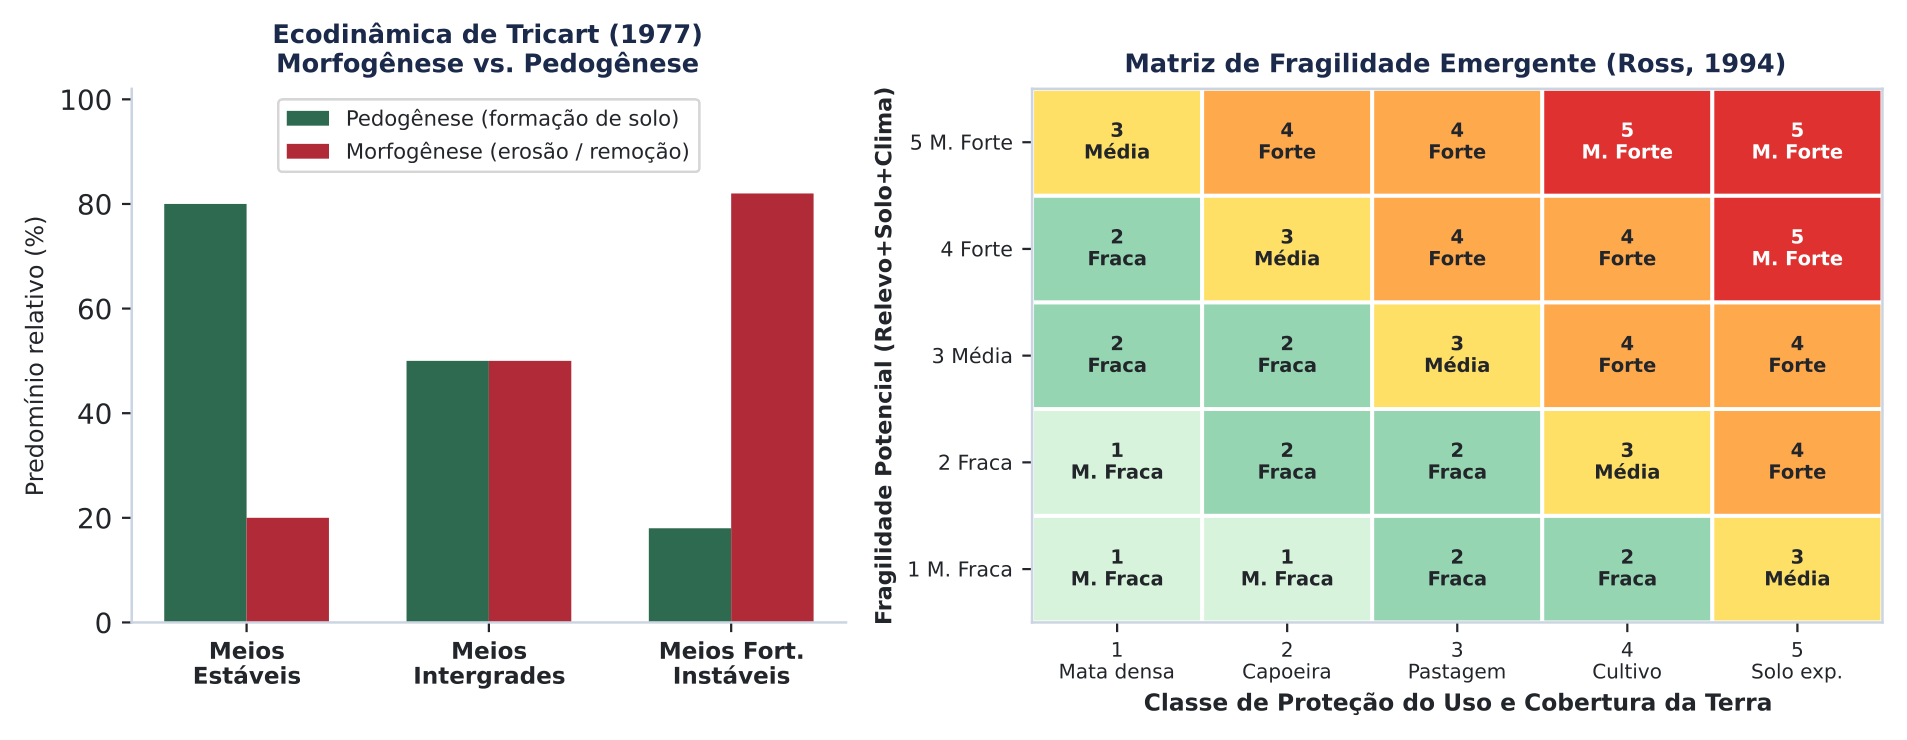
\includegraphics[keepaspectratio]{capitulos/../img/fig07_ecodinamica_ross_matriz.png}}

}

\caption{\label{fig-ecodinamica_ross}Integração metodológica entre a
Ecodinâmica de Tricart (1977), expressa pelo balanço relativo entre
pedogênese e morfogênese nos três tipos de meios (Painel A), e a Matriz
de Fragilidade Emergente de Ross (1994), obtida pelo cruzamento da
Fragilidade Potencial com o grau de proteção do Uso da Terra (Painel
B).}

\end{figure}%

\subsection{Análise Empírica da Fragilidade Ambiental (Ross,
1994)}\label{anuxe1lise-empuxedrica-da-fragilidade-ambiental-ross-1994}

Na década de 1990, o geógrafo brasileiro \textbf{Jurandyr Luciano
Sanches Ross (1994)} operacionalizou os princípios dos Geossistemas e da
Ecodinâmica de Tricart em uma metodologia cartográfica e quantitativa
padronizada, a \textbf{Análise Empírica da Fragilidade dos Ambientes
Naturais e Antropizados}. Para manter a coerência com Tricart, Ross
substituiu a expressão ``meios estáveis/instáveis'' por \textbf{Unidades
Ecodinâmicas Estáveis} e \textbf{Unidades Ecodinâmicas de Instabilidade
Potencial ou Emergente}, classificadas em \textbf{cinco graus
hierárquicos},

\[
1 = \text{Muito Fraca} \quad;\quad 2 = \text{Fraca} \quad;\quad 3 = \text{Média} \quad;\quad 4 = \text{Forte} \quad;\quad 5 = \text{Muito Forte}.
\]

\subsection{Distinção Fundamental, Fragilidade Potencial vs.~Fragilidade
Emergente}\label{distinuxe7uxe3o-fundamental-fragilidade-potencial-vs.-fragilidade-emergente}

\textbf{Fragilidade Potencial (\(FP\)).} Expressa a suscetibilidade
\emph{natural e intrínseca} do terreno antes de considerar a ação humana
ou a vegetação atual. Combina exclusivamente os fatores do meio físico,
\textbf{Relevo/Declividade (\(D_R\))}, \textbf{Solos (\(D_S\))} e
\textbf{Clima/Pluviosidade (\(D_C\))}. Responde à pergunta, \emph{``Quão
vulnerável este terreno seria se perdesse sua cobertura vegetal?''}.
\textbf{Fragilidade Emergente (\(FE\)).} Expressa a suscetibilidade
\emph{real e atual} do ambiente, resultando do cruzamento entre a
\textbf{Fragilidade Potencial (\(FP\))} e o grau de proteção oferecido
pelo \textbf{Uso da Terra / Cobertura Vegetal (\(D_U\))}. Responde à
pergunta, \emph{``Qual é o risco efetivo de degradação hoje,
considerando o uso e a vegetação existentes?''}.

\subsubsection{Tabelas Completas das Cinco Classes Hierárquicas de Ross
(1994)}\label{tabelas-completas-das-cinco-classes-hieruxe1rquicas-de-ross-1994}

As Tabelas~\hyperref[tbl-ross_relevo_solos]{ross relevo solos}
e~\hyperref[tbl-ross_clima_uso]{ross clima uso} apresentam os critérios
completos das quatro variáveis básicas utilizadas na metodologia de Ross
(1994). Em estudos de detalhe (microbacias e municípios, escalas de
\(1:10.000\) a \(1:50.000\)), adota-se a \textbf{declividade (\(S\%\))}
como indicador do relevo; em estudos regionais (escalas menores que
\(1:100.000\)), utilizam-se os índices de dissecação do relevo
(entalhamento de vales e dimensão interfluvial).

\begin{longtable}[]{@{}
  >{\raggedright\arraybackslash}p{(\linewidth - 6\tabcolsep) * \real{0.2500}}
  >{\raggedright\arraybackslash}p{(\linewidth - 6\tabcolsep) * \real{0.2500}}
  >{\raggedright\arraybackslash}p{(\linewidth - 6\tabcolsep) * \real{0.2500}}
  >{\raggedright\arraybackslash}p{(\linewidth - 6\tabcolsep) * \real{0.2500}}@{}}
\caption{Classes hierárquicas de fragilidade para Relevo/Declividade
(\(D_R\)) e Solos (\(D_S\)) segundo Ross
(1994).}\label{tbl-ross_relevo_solos}\tabularnewline
\toprule\noalign{}
\begin{minipage}[b]{\linewidth}\raggedright
\textbf{Classe / Grau}
\end{minipage} & \begin{minipage}[b]{\linewidth}\raggedright
\textbf{Declividade (\(D_R\))}
\end{minipage} & \begin{minipage}[b]{\linewidth}\raggedright
\textbf{Dissecação Regional (\(D_R\))}
\end{minipage} & \begin{minipage}[b]{\linewidth}\raggedright
\textbf{Classes de Solos / Erodibilidade (\(D_S\))}
\end{minipage} \\
\midrule\noalign{}
\endfirsthead
\toprule\noalign{}
\begin{minipage}[b]{\linewidth}\raggedright
\textbf{Classe / Grau}
\end{minipage} & \begin{minipage}[b]{\linewidth}\raggedright
\textbf{Declividade (\(D_R\))}
\end{minipage} & \begin{minipage}[b]{\linewidth}\raggedright
\textbf{Dissecação Regional (\(D_R\))}
\end{minipage} & \begin{minipage}[b]{\linewidth}\raggedright
\textbf{Classes de Solos / Erodibilidade (\(D_S\))}
\end{minipage} \\
\midrule\noalign{}
\endhead
\bottomrule\noalign{}
\endlastfoot
\textbf{1, Muito Fraca} & \(< 6\%\) & Muito fraca (vales muito rasos,
interflúvios amplos) & Latossolos Roxos e Vermelho-Escuros de textura
argilosa (muito profundos e bem estruturados). \\
\textbf{2, Fraca} & \(6\text{ a } 12\%\) & Fraca (entalhamento e
densidade baixos) & Latossolos Vermelho-Amarelos de textura
média/argilosa; Nitossolos profundos. \\
\textbf{3, Média} & \(12\text{ a } 20\%\) & Média (vertentes
moderadamente dissecadas) & Latossolos Amarelos/Vermelho-Amarelos
arenosos; Argissolos profundos; Cambissolos profundos. \\
\textbf{4, Forte} & \(20\text{ a } 30\%\) & Forte (vales entalhados e
interflúvios estreitos) & Argissolos com mudança textural abrupta;
Planossolos (comum no Semiárido); Cambissolos rasos/siltosos. \\
\textbf{5, Muito Forte} & \(> 30\%\) & Muito forte (escarpas, vales
muito profundos) & Neossolos Litólicos (solos rasos sobre rocha),
Neossolos Quartzarênicos (areias quartzosas), Gleissolos e Organossolos
em áreas instáveis. \\
\end{longtable}

\begin{longtable}[]{@{}
  >{\raggedright\arraybackslash}p{(\linewidth - 4\tabcolsep) * \real{0.3333}}
  >{\raggedright\arraybackslash}p{(\linewidth - 4\tabcolsep) * \real{0.3333}}
  >{\raggedright\arraybackslash}p{(\linewidth - 4\tabcolsep) * \real{0.3333}}@{}}
\caption{Classes hierárquicas de fragilidade para Clima/Pluviosidade
(\(D_C\)) e Uso da Terra / Cobertura Vegetal (\(D_U\)) segundo Ross
(1994).}\label{tbl-ross_clima_uso}\tabularnewline
\toprule\noalign{}
\begin{minipage}[b]{\linewidth}\raggedright
\textbf{Classe / Grau}
\end{minipage} & \begin{minipage}[b]{\linewidth}\raggedright
\textbf{Clima / Pluviosidade (\(D_C\), Erosividade)}
\end{minipage} & \begin{minipage}[b]{\linewidth}\raggedright
\textbf{Uso da Terra / Cobertura Vegetal (\(D_U\), Grau de Proteção)}
\end{minipage} \\
\midrule\noalign{}
\endfirsthead
\toprule\noalign{}
\begin{minipage}[b]{\linewidth}\raggedright
\textbf{Classe / Grau}
\end{minipage} & \begin{minipage}[b]{\linewidth}\raggedright
\textbf{Clima / Pluviosidade (\(D_C\), Erosividade)}
\end{minipage} & \begin{minipage}[b]{\linewidth}\raggedright
\textbf{Uso da Terra / Cobertura Vegetal (\(D_U\), Grau de Proteção)}
\end{minipage} \\
\midrule\noalign{}
\endhead
\bottomrule\noalign{}
\endlastfoot
\textbf{1, Muito Fraca} & Pluviosidade regular ao longo do ano, baixa
intensidade horária, sem concentração extrema. & \textbf{Proteção Muito
Alta.} Florestas naturais primárias, matas ciliares densas e Caatinga
arbórea fechada. \\
\textbf{2, Fraca} & Precipitação moderada
(\(1.000\text{-}1.300\text{ mm/ano}\)) com estação seca curta e chuvas
pouco torrenciais. & \textbf{Proteção Alta.} Florestas secundárias
avançadas (capoeirões), Caatinga arbustivo-arbórea densa, silvicultura
bem manejada. \\
\textbf{3, Média} & Estação seca definida (\(3\text{-}6\) meses) e
chuvas concentradas no verão/outono com eventos erosivos moderados. &
\textbf{Proteção Média.} Pastagens bem manejadas com boa cobertura,
sistemas agroflorestais (SAFs), culturas perenes (café, cacau em
cabruca). \\
\textbf{4, Forte} & Forte concentração pluviométrica sazonal (ou totais
\(>2.000\text{ mm/ano}\) com aguaceiros intensos). & \textbf{Proteção
Baixa.} Culturas temporárias de ciclo curto (milho, feijão, mandioca),
pastagens degradadas/raleadas e áreas de queimada antiga. \\
\textbf{5, Muito Forte} & Chuvas altamente concentradas e torrenciais
(típico do Semiárido com aguaceiros sobre solo seco, ou áreas de extrema
erosividade). & \textbf{Proteção Muito Baixa / Nula.} Solo exposto,
áreas terraplanadas, mineração, queimada recente, área urbana sem
drenagem. \\
\end{longtable}

\subsubsection{\texorpdfstring{Cálculo e Leitura do Código Numérico de
Ross (\(FP\) e
\(FE\))}{Cálculo e Leitura do Código Numérico de Ross (FP e FE)}}\label{cuxe1lculo-e-leitura-do-cuxf3digo-numuxe9rico-de-ross-fp-e-fe}

Na metodologia de Ross (1994), cada unidade geoambiental recebe um
\textbf{código numérico posicional} que preserva a memória individual de
cada variável, impedindo que a causa do problema desapareça na média,

\textbf{Código da Fragilidade Potencial (\(FP\)).} Formado por
\textbf{três dígitos} na ordem fixa \(\mathbf{D_R\,D_S\,D_C}\) (Relevo,
Solos, Clima). \textbf{Código da Fragilidade Emergente (\(FE\)).}
Formado por \textbf{quatro dígitos} na ordem fixa
\(\mathbf{D_R\,D_S\,D_C\,D_U}\) (Relevo, Solos, Clima, Uso da Terra).

\subsection{\texorpdfstring{Cálculo e Leitura da Fragilidade Potencial
(\(FP\)) e Fragilidade Emergente
(\(FE\))}{Cálculo e Leitura da Fragilidade Potencial (FP) e Fragilidade Emergente (FE)}}\label{cuxe1lculo-e-leitura-da-fragilidade-potencial-fp-e-fragilidade-emergente-fe}

\textbf{Passo 1, Atribuição dos dígitos (\(1\) a \(5\)).} Enquadre o
terreno nas Tabelas~\hyperref[tbl-ross_relevo_solos]{ross relevo solos}
e~\hyperref[tbl-ross_clima_uso]{ross clima uso}, obtendo \(D_R\),
\(D_S\), \(D_C\) e \(D_U\).

\textbf{Passo 2, Montagem dos códigos posicionais,}

\[
\text{Código } FP = D_R\,D_S\,D_C \qquad\text{e}\qquad \text{Código } FE = D_R\,D_S\,D_C\,D_U.
\]

\textbf{Passo 3, Determinação da Classe Síntese de \(FP\) (1 a 5).}
Calcula-se a média aritmética das três variáveis físicas e arredonda-se
para o inteiro mais próximo de \(1\) a \(5\) (em empates de \(0{,}5\),
adota-se o valor mais conservador ou o peso dominante do relevo
\(D_R\)),

\[
I_{FP} = \frac{D_R + D_S + D_C}{3} \quad \xrightarrow{\text{arredondamento}} \quad \text{Classe } FP \in \{1, 2, 3, 4, 5\}.
\]

\textbf{Passo 4, Determinação da Classe Síntese de \(FE\) (1 a 5) na
Matriz de Fragilidade Emergente.} Cruza-se a \textbf{Classe \(FP\)}
(linha) com o dígito do \textbf{Uso da Terra \(D_U\)} (coluna) na
adaptação didático-operacional da matriz de Ross (1994) e Spörl e Ross
(2004) apresentada abaixo (Figura~\ref{fig-ecodinamica_ross}, Painel B).
Nos casos em que \((FP + D_U)/2\) resulta em fração \(0{,}5\), a matriz
pondera o efeito protetor da cobertura vegetal densa (\(D_U \le 2\),
arredondando para baixo) em contraste com o agravamento imposto por usos
antrópicos expostos (\(D_U \ge 3\), arredondando para cima),

{\def\LTcaptype{none} % do not increment counter
\begin{longtable}[]{@{}
  >{\raggedright\arraybackslash}p{(\linewidth - 10\tabcolsep) * \real{0.1667}}
  >{\raggedright\arraybackslash}p{(\linewidth - 10\tabcolsep) * \real{0.1667}}
  >{\raggedright\arraybackslash}p{(\linewidth - 10\tabcolsep) * \real{0.1667}}
  >{\raggedright\arraybackslash}p{(\linewidth - 10\tabcolsep) * \real{0.1667}}
  >{\raggedright\arraybackslash}p{(\linewidth - 10\tabcolsep) * \real{0.1667}}
  >{\raggedright\arraybackslash}p{(\linewidth - 10\tabcolsep) * \real{0.1667}}@{}}
\toprule\noalign{}
\begin{minipage}[b]{\linewidth}\raggedright
\textbf{Fragilidade Potencial (\(FP\))} \(\backslash\) \textbf{Uso
(\(D_U\))}
\end{minipage} & \begin{minipage}[b]{\linewidth}\raggedright
\textbf{1 (M. Alta Prot.)}
\end{minipage} & \begin{minipage}[b]{\linewidth}\raggedright
\textbf{2 (Alta)}
\end{minipage} & \begin{minipage}[b]{\linewidth}\raggedright
\textbf{3 (Média)}
\end{minipage} & \begin{minipage}[b]{\linewidth}\raggedright
\textbf{4 (Baixa)}
\end{minipage} & \begin{minipage}[b]{\linewidth}\raggedright
\textbf{5 (Nula)}
\end{minipage} \\
\midrule\noalign{}
\endhead
\bottomrule\noalign{}
\endlastfoot
\textbf{1, Muito Fraca} & 1 (M. Fraca) & 1 (M. Fraca) & 2 (Fraca) & 2
(Fraca) & 3 (Média) \\
\textbf{2, Fraca} & 1 (M. Fraca) & 2 (Fraca) & 2 (Fraca) & 3 (Média) & 4
(Forte) \\
\textbf{3, Média} & 2 (Fraca) & 2 (Fraca) & 3 (Média) & 4 (Forte) & 4
(Forte) \\
\textbf{4, Forte} & 2 (Fraca) & 3 (Média) & 4 (Forte) & 4 (Forte) & 5
(M. Forte) \\
\textbf{5, Muito Forte} & 3 (Média) & 4 (Forte) & 4 (Forte) & 5 (M.
Forte) & 5 (M. Forte) \\
\end{longtable}
}

\emph{Nota,} na célula \((FP=5, D_U=1)\), a proteção florestal primária
reduz a fragilidade emergente para \textbf{3, Média}.

\textbf{Exemplo numérico completo.} Uma encosta com declividade
\(S = 22\%\) (\(D_R = 4\)), Argissolo profundo (\(D_S = 3\)), clima
semiárido com chuvas torrenciais concentradas (\(D_C = 4\)) e pastagem
degradada (\(D_U = 4\)),

\textbf{Código \(FP\),} \(\mathbf{434}\). Média
\(I_{FP} = (4 + 3 + 4)/3 = 11/3 \approx 3{,}67 \implies\) \textbf{Classe
\(FP = 4\) (Forte)}. \textbf{Código \(FE\),} \(\mathbf{4344}\). Cruzando
\(FP = 4\) com \(D_U = 4\) na matriz acima \(\implies\) \textbf{Classe
\(FE = 4\) (Forte)}. \textbf{Leitura técnica do código \(4344\).} O
primeiro dígito (\(4\)) alerta que a declividade (\(20\text{-}30\%\)) é
o principal motor físico; o terceiro (\(4\)) indica forte erosividade
climática; o quarto (\(4\)) revela que a pastagem degradada não protege
o solo, mantendo o risco real elevado (Classe 4).

\subsection{Classes de fragilidade e verificação dos
mecanismos}\label{classes-de-fragilidade-e-verificauxe7uxe3o-dos-mecanismos}

Classes de 1 a 5 organizam níveis de suscetibilidade segundo uma
convenção. A distância entre duas classes consecutivas não representa
necessariamente o mesmo incremento físico de erosão. O cruzamento de
classes precisa ser apresentado junto à regra de combinação e às
condições que justificam sua utilização.

As médias, matrizes e regras de arredondamento empregadas nesta apostila
constituem adaptações didáticas. Sua atribuição deve distinguir a
abordagem conceitual de Ross dos procedimentos construídos para os
exercícios. Uma mudança nos pesos ou na regra de combinação pode alterar
a classificação final, motivo pelo qual a análise de sensibilidade faz
parte da interpretação.

A cobertura vegetal pode reduzir o impacto das gotas e proteger a
superfície, enquanto processos profundos dependem também de materiais,
poropressão e geometria da encosta. Uma classe emergente mais baixa por
efeito da cobertura deve ser interpretada conforme o processo analisado.
A conservação da vegetação não fornece, isoladamente, uma estimativa de
estabilidade geotécnica.

A conferência em campo confronta o mapa com incisões ativas, surgências,
depósitos recentes e alterações da drenagem. Divergências ajudam a
revisar o modelo e podem indicar que uma variável relevante foi omitida
ou que a escala cartográfica ocultou uma condição local.

\section{Etapa 4 - Exemplos
resolvidos}\label{etapa-4---exemplos-resolvidos-8}

\subsection{Exemplo 9.1 - Enquadramento na Taxonomia da Paisagem de
Bertrand (Nível
Básico)}\label{exemplo-9.1---enquadramento-na-taxonomia-da-paisagem-de-bertrand-nuxedvel-buxe1sico}

\textbf{Situação analisada.} Uma equipe de Análise Ambiental da UEFS
está diagnosticando processos erosivos em uma propriedade rural próxima
a Feira de Santana (BA). Durante o trabalho, os estudantes precisam
situar espacialmente quatro recortes, (I) o Domínio das Caatingas; (II)
a sub-bacia do Rio Jacuípe (escala \(1:100.000\)); (III) uma vertente
homogênea de pastagem sobre Argissolo (\(1:15.000\)); e (IV) uma
voçoroca ativa com \(40\,\text{m}\) de comprimento (\(1:1.000\)).

\textbf{Dados disponíveis.} Quatro recortes espaciais com escalas
variando de continental/regional (\(G\text{II}\)) até o detalhe local
(\(G\text{VII}\)).

\textbf{Problema a resolver.} Enquadrar corretamente cada recorte (I a
IV) nas unidades taxonômicas de Bertrand (2004).

\textbf{Fundamento da análise.} Aplicação direta da
Tabela~\hyperref[tbl-taxonomia_bertrand]{taxonomia bertrand} (unidades
superiores e inferiores segundo ordem de grandeza e critério definidor).

\textbf{Desenvolvimento.}

\textbf{Recorte I (Domínio das Caatingas).} Escala
regional/subcontinental (\(G\text{II}\), \(\sim 10^6\text{ km}^2\))
definida por macroclima e bioma \(\implies\) \textbf{Domínio}.
\textbf{Recorte II (Sub-bacia em \(1:100.000\)).} Unidade funcional
concreta (\(G\text{V}\), dezenas a centenas de \(\text{km}^2\)) que
integra potencial ecológico, exploração biológica e ação antrópica
\(\implies\) \textbf{Geossistema}. \textbf{Recorte III (Vertente
homogênea em \(1:15.000\)).} Setor fisionomicamente uniforme dentro do
geossistema (\(G\text{VI}\)) \(\implies\) \textbf{Geofácies}.
\textbf{Recorte IV (Voçoroca de \(40\,\text{m}\) em \(1:1.000\)).} Menor
unidade espacial de detalhe extremo (\(G\text{VII}\)) \(\implies\)
\textbf{Geótopo}.

\textbf{Interpretação do resultado.} I = Domínio; II = Geossistema; III
= Geofácies; IV = Geótopo.

\textbf{Condições de validade.} A sequência segue exatamente a ordem
decrescente de grandeza espacial da taxonomia de Bertrand
(\(G\text{II} \to G\text{V} \to G\text{VI} \to G\text{VII}\)), evitando
misturar unidades regionais com feições pontuais de campo.

\subsection{Exemplo 9.2 - Diagnóstico Ecodinâmico de Tricart em Três
Setores de Sub-bacia (Nível
Básico-Intermediário)}\label{09-geossistemas-ecodinamica-ross-exemplo-9.2.-diagnuxf3stico-ecodinuxe2mico-de-tricart-em-truxeas-setores-de-sub-bacia-nuxedvel-buxe1sicointermediuxe1rio}

\textbf{Situação analisada.} Ao percorrer uma sub-bacia do Piemonte da
Chapada Diamantina, um geógrafo observou três compartimentos distintos,
\textbf{Setor X}, chapada plana com vegetação arbórea conservada,
Latossolo profundo e ausência de sulcos; \textbf{Setor Y}, rampa suave
(\(9\%\)) com pastagem manejada, onde ocorrem infiltração moderada e
leve escoamento laminar após chuvas fortes; \textbf{Setor Z}, encosta
íngreme (\(35\%\)) desmatada, com Neossolo Litólico raso, ravinas
profundas e blocos rolados.

\textbf{Dados disponíveis.} Setor X (plano, florestado, solo profundo);
Setor Y (\(S=9\%\), pastagem, erosão laminar leve); Setor Z (\(S=35\%\),
desmatado, solo raso, ravinas).

\textbf{Problema a resolver.} Classificar cada setor segundo a
Ecodinâmica de Tricart (1977), explicando o balanço morfogênese
vs.~pedogênese.

\textbf{Fundamento da análise.} Comparação dos processos dominantes com
os critérios da Tabela~\hyperref[tbl-ecodinamica_tricart]{ecodinamica
tricart} e do Painel A da Figura~\ref{fig-ecodinamica_ross}.

\textbf{Desenvolvimento.}

\textbf{Setor X.} A cobertura arbórea e o relevo plano maximizam a
infiltração e o intemperismo químico profundo, bloqueando a erosão
superficial (\(P \gg M\)) \(\implies\) \textbf{Meio Estável}.
\textbf{Setor Y.} Há competição equilibrada entre infiltração sob
pastagem e remoção laminar nas chuvas intensas (\(P \approx M\))
\(\implies\) \textbf{Meio Intergrade (de Transição)}. \textbf{Setor Z.}
A alta declividade aliada à remoção da vegetação dispara erosão linear e
perda acelerada de solo (\(M \gg P\)) \(\implies\) \textbf{Meio
Fortemente Instável}.

\textbf{Interpretação do resultado.} Setor X = Meio Estável; Setor Y =
Meio Intergrade; Setor Z = Meio Fortemente Instável.

\textbf{Condições de validade.} O diagnóstico orienta diretamente a
gestão, no Setor Z a prioridade é contenção erosiva e revegetação; no
Setor Y, manejo conservacionista para impedir que o meio intergrade
migre para a instabilidade forte.

\subsection{Exemplo 9.3 - Cálculo Passo a Passo da Fragilidade Potencial
e Emergente (Nível
Intermediário)}\label{exemplo-9.3---cuxe1lculo-passo-a-passo-da-fragilidade-potencial-e-emergente-nuxedvel-intermediuxe1rio}

\textbf{Situação analisada.} Uma unidade geoambiental utilizada para
estudo de planejamento municipal apresenta declividade média de
\(S = 15\%\), solo classificado como Argissolo profundo de textura
média/argilosa, clima tropical semiárido com chuvas concentradas e
torrenciais (\(D_C = 4\)) e uso atual por cultura temporária de mandioca
em solo parcialmente descoberto.

\textbf{Dados disponíveis.} \(S = 15\%\); Argissolo profundo;
\(D_C = 4\); uso por cultura temporária de ciclo curto.

\textbf{Problema a resolver.} Determinar os dígitos \(D_R\), \(D_S\),
\(D_C\) e \(D_U\), montar os códigos numéricos de \(FP\) e \(FE\) e
obter as classes síntese de Fragilidade Potencial e Emergente.

\textbf{Fundamento da análise.} Enquadramento pelas
Tabelas~\hyperref[tbl-ross_relevo_solos]{ross relevo solos}
e~\hyperref[tbl-ross_clima_uso]{ross clima uso} e aplicação do roteiro
de cálculo de Ross (1994).

\textbf{Desenvolvimento.}

Relevo (\(S = 15\%\), faixa \(12\text{-}20\%\)), \(D_R = 3\) (Média).
Solos (Argissolo profundo), \(D_S = 3\) (Média). Clima (fornecido),
\(D_C = 4\) (Forte). Uso da Terra (cultura temporária de ciclo curto),
\(D_U = 4\) (Proteção Baixa / Fragilidade Forte).

\textbf{Atribuição dos dígitos,}. \textbf{Fragilidade Potencial
(\(FP\)).} Código posicional \(\mathbf{334}\). Média física,

\[
I_{FP} = \frac{3 + 3 + 4}{3} = \frac{10}{3} \approx 3{,}33 \implies \text{Classe } FP = \mathbf{3\text{ (Média)}}.
\]

. \textbf{Fragilidade Emergente (\(FE\)).} Código posicional
\(\mathbf{3344}\). Cruzando \(FP = 3\) com \(D_U = 4\) na Matriz de Ross
(Figura~\ref{fig-ecodinamica_ross}, Painel B) \(\implies\)
\textbf{Classe \(FE = 4\) (Forte)}.

\textbf{Interpretação do resultado.} Código \(FP = 334\) (Classe 3,
Média); Código \(FE = 3344\) (Classe 4, Forte).

\textbf{Condições de validade.} Note o papel agravante do uso agrícola
anual (\(D_U = 4\)), a unidade possui fragilidade natural média (\(3\)),
mas o cultivo temporário com baixa proteção eleva a fragilidade real
emergente para forte (\(4\)), exigindo plantio em nível e cobertura
morta.

\subsection{Exemplo 9.4 - Efeito Amortecedor da Vegetação na Matriz de
Ross (Nível
Intermediário-Avançado)}\label{09-geossistemas-ecodinamica-ross-exemplo-9.4.-efeito-amortecedor-da-vegetauxe7uxe3o-na-matriz-de-ross-nuxedvel-intermediuxe1rioavanuxe7ado}

\textbf{Situação analisada.} Considere uma encosta íngreme de
\(S = 24\%\) (\(D_R = 4\)) com Planossolo/Argissolo abrúptico
(\(D_S = 4\)) sob regime de chuvas intensas sazonais (\(D_C = 4\)).
Compare dois cenários de uso sobre essa mesma base física,
\textbf{Cenário 1}, área mantida com mata nativa primária densa;
\textbf{Cenário 2}, área totalmente desmatada e terraplanada (solo
exposto) para loteamento sem drenagem.

\textbf{Dados disponíveis.} \(D_R = 4\), \(D_S = 4\), \(D_C = 4\).
Cenário 1, mata primária densa. Cenário 2, solo exposto/terraplanagem.

\textbf{Problema a resolver.} Calcular \(FP\) e \(FE\) para ambos os
cenários e explicar tecnicamente a diferença obtida.

\textbf{Fundamento da análise.} Cálculo do código \(FP\), identificação
de \(D_U\) pela Tabela~\hyperref[tbl-ross_clima_uso]{ross clima uso} e
leitura da Matriz de Fragilidade Emergente de Ross.

\textbf{Desenvolvimento.}

\textbf{Fragilidade Potencial (\(FP\), idêntica nos dois cenários).}
Código \(\mathbf{444}\); \(I_{FP} = (4+4+4)/3 = 4{,}0 \implies\)
\textbf{Classe \(FP = 4\) (Forte)}. \textbf{Cenário 1 (mata nativa densa
\(\implies D_U = 1\)).} Código \(FE = \mathbf{4441}\). Na Matriz de
Ross, o cruzamento \(FP = 4 \times D_U = 1\) resulta em \textbf{Classe
\(FE = 2\) (Fraca)}. \textbf{Cenário 2 (solo exposto
\(\implies D_U = 5\)).} Código \(FE = \mathbf{4445}\). Na Matriz de
Ross, o cruzamento \(FP = 4 \times D_U = 5\) resulta em \textbf{Classe
\(FE = 5\) (Muito Forte)}.

\textbf{Interpretação do resultado.} Ambos têm \(FP = 444\) (Classe 4,
Forte). No Cenário 1, \(FE = 4441\) (Classe 2, Fraca); no Cenário 2,
\(FE = 4445\) (Classe 5, Muito Forte).

\textbf{Condições de validade.} O resultado comprova quantitativamente o
princípio de Ross e Tricart, a floresta densa reduz em dois graus a
fragilidade emergente (\(4 \to 2\)), mantendo o equilíbrio pedogenético;
já a exposição do solo libera toda a energia potencial da encosta,
disparando a fragilidade máxima (\(5\)).

\subsection{Exemplo 9.5 - Compartimentação Geoambiental e Zoneamento de
Microbacia (Nível
Avançado)}\label{exemplo-9.5---compartimentauxe7uxe3o-geoambiental-e-zoneamento-de-microbacia-nuxedvel-avanuxe7ado}

\textbf{Situação analisada.} Para elaborar o diagnóstico
físico-ambiental do Trabalho Prático Final, uma microbacia do Semiárido
baiano (\(D_C = 4\) em toda a área) foi compartimentada em três Unidades
Geoambientais (UGs),

\textbf{UG1 (Topo de Tabuleiro),} \(S = 3\%\), Latossolo Vermelho-Escuro
argiloso, Caatinga arbustivo-arbórea densa;. \textbf{UG2 (Meia Encosta
Dissecada),} \(S = 35\%\), Neossolo Litólico, pastagem degradada;.
\textbf{UG3 (Sopé Coluvial),} \(S = 9\%\), Planossolo, sistema
agroflorestal (SAF) manejado.

\textbf{Dados disponíveis.} UG1 (\(S=3\%\), Latossolo argiloso, Caatinga
densa); UG2 (\(S=35\%\), Neossolo Litólico, pastagem degradada); UG3
(\(S=9\%\), Planossolo, SAF manejado); \(D_C = 4\) em toda a microbacia.

\textbf{Problema a resolver.} Calcular o código \(FP\), a classe \(FP\),
o código \(FE\), a classe \(FE\) e o meio ecodinâmico de Tricart para
cada UG, propondo diretrizes de ordenamento.

\textbf{Fundamento da análise.} Integração das
Tabelas~\hyperref[tbl-ecodinamica_tricart]{ecodinamica tricart},
\hyperref[tbl-ross_relevo_solos]{ross relevo solos}
e~\hyperref[tbl-ross_clima_uso]{ross clima uso} e da Matriz de Ross.

\textbf{Desenvolvimento.}

\textbf{UG1 (Topo),} \(D_R=1\), \(D_S=1\), \(D_C=4\), \(D_U=2\). Código
\(FP = \mathbf{114}\),
\(I_{FP} = (1+1+4)/3 = 2{,}0 \implies FP = \mathbf{2}\) (Fraca). Código
\(FE = \mathbf{1142}\); cruzando
\(FP=2 \times D_U=2 \implies FE = \mathbf{2}\) (Fraca). Meio
\textbf{Estável}. \textbf{UG2 (Meia Encosta),} \(D_R=5\), \(D_S=5\),
\(D_C=4\), \(D_U=4\). Código \(FP = \mathbf{554}\),
\(I_{FP} = (5+5+4)/3 = 14/3 \approx 4{,}67 \implies FP = \mathbf{5}\)
(Muito Forte). Código \(FE = \mathbf{5544}\); cruzando
\(FP=5 \times D_U=4 \implies FE = \mathbf{5}\) (Muito Forte). Meio
\textbf{Fortemente Instável}. \textbf{UG3 (Sopé),} \(D_R=2\), \(D_S=4\),
\(D_C=4\), \(D_U=3\). Código \(FP = \mathbf{244}\),
\(I_{FP} = (2+4+4)/3 = 10/3 \approx 3{,}33 \implies FP = \mathbf{3}\)
(Média). Código \(FE = \mathbf{2443}\); cruzando
\(FP=3 \times D_U=3 \implies FE = \mathbf{3}\) (Média). Meio
\textbf{Intergrade}.

\textbf{Interpretação do resultado.} UG1, \(FP=114\) (2), \(FE=1142\)
(2, Fraca, Estável); UG2, \(FP=554\) (5), \(FE=5544\) (5, Muito Forte,
Fortemente Instável); UG3, \(FP=244\) (3), \(FE=2443\) (3, Média,
Intergrade).

\textbf{Condições de validade.} O zoneamento resultante é ambientalmente
coerente, UG1 comporta uso sustentável controlado; UG3 exige manejo
conservacionista (manutenção do SAF e drenagem do Planossolo); UG2 deve
ser destinada à preservação e recuperação (exclusão do gado e
bioengenharia para conter ravinas).

\section{Etapa 5 - Erros de
interpretação}\label{etapa-5---erros-de-interpretauxe7uxe3o-8}

\subsection{\texorpdfstring{Erro 1, Confundir Fragilidade Potencial
(\(FP\)) com Fragilidade Emergente
(\(FE\))}{Erro 1, Confundir Fragilidade Potencial (FP) com Fragilidade Emergente (FE)}}\label{erro-1-confundir-fragilidade-potencial-fp-com-fragilidade-emergente-fe}

\textbf{Equívoco frequente.} Incluir o uso da terra (\(D_U\)) no cálculo
da Fragilidade Potencial, ou afirmar que uma encosta íngreme florestada
tem ``baixa fragilidade potencial''.

\textbf{Correção técnica.} A \textbf{Fragilidade Potencial (\(FP\))}
depende exclusivamente dos fatores físicos naturais (\(D_R, D_S, D_C\)).
Uma encosta de \(35\%\) com solo raso continua tendo \textbf{FP Muito
Forte (\(5\))} mesmo sob mata primária; o que a floresta reduz é a
\textbf{Fragilidade Emergente (\(FE\))}, que passa a depender do uso
atual (\(D_U\)).

\subsection{\texorpdfstring{Erro 2, Inverter a escala de proteção do Uso
da Terra (\(D_U\)) em Ross
(1994)}{Erro 2, Inverter a escala de proteção do Uso da Terra (D\_U) em Ross (1994)}}\label{erro-2-inverter-a-escala-de-proteuxe7uxe3o-do-uso-da-terra-d_u-em-ross-1994}

\textbf{Equívoco frequente.} Atribuir classe \(5\) para floresta densa
(por associar \(5\) ao ``máximo de vegetação'') e classe \(1\) para solo
exposto.

\textbf{Correção técnica.} Na metodologia de Ross, \textbf{todas as
variáveis seguem o sentido da fragilidade} (\(1\) = menor fragilidade;
\(5\) = maior fragilidade). Portanto, a floresta densa, por oferecer
máxima proteção contra a erosão, recebe \textbf{classe \(1\)}, enquanto
o solo exposto recebe \textbf{classe \(5\)}.

\subsection{Erro 3, Tratar ``Meio Intergrade'' como sinônimo de ``Meio
Sem
Risco''}\label{erro-3-tratar-meio-intergrade-como-sinuxf4nimo-de-meio-sem-risco}

\textbf{Equívoco frequente.} Concluir que ambientes intergrades de
Tricart são estáveis e dispensam práticas de manejo.

\textbf{Correção técnica.} O meio intergrade é uma \textbf{zona de
transição dinâmica} (\(P \approx M\)). Basta uma intervenção inadequada
(queimada, sobrepastejo ou corte de talude) para que a morfogênese
supere a pedogênese e o setor passe rapidamente a fortemente instável.

\subsection{Erro 4, Usar Geossistema e Ecossistema como termos idênticos
sem critério
escalar}\label{erro-4-usar-geossistema-e-ecossistema-como-termos-iduxeanticos-sem-crituxe9rio-escalar}

\textbf{Equívoco frequente.} Chamar qualquer parcela de
\(10\text{ m}^2\) ou um bioma continental inteiro de ``geossistema''.

\textbf{Correção técnica.} Na taxonomia de Bertrand (2004), o
geossistema ocupa a ordem \(G\text{V}\) (escala de dezenas a centenas de
\(\text{km}^2\), cartas de \(1:50.000\) a \(1:100.000\)). Unidades
continentais pertencem à Zona/Domínio (\(G\text{I}\text{-}G\text{II}\)),
e unidades pontuais de campo pertencem ao Geótopo (\(G\text{VII}\)).

\section{Etapa 6 - Exercícios de
fixação}\label{etapa-6---exercuxedcios-de-fixauxe7uxe3o-8}

\subsubsection{Nível Básico (Exercícios 1 a
5)}\label{nuxedvel-buxe1sico-exercuxedcios-1-a-5-4}

\begin{enumerate}
\def\labelenumi{\arabic{enumi}.}
\item
  Explique, com base na Teoria Geral dos Sistemas (Bertalanffy, 2010),
  por que a fragilidade ambiental é considerada uma \textbf{propriedade
  emergente} da paisagem e não uma característica isolada de um único
  elemento físico.
\item
  Liste em ordem decrescente de escala espacial as seis unidades
  taxonômicas da paisagem propostas por Bertrand (2004), separando as
  unidades superiores das unidades inferiores.
\item
  Defina \textbf{morfogênese} e \textbf{pedogênese} segundo Tricart
  (1977) e indique qual processo predomina nos meios estáveis e nos
  meios fortemente instáveis.
\item
  Um terreno possui \(D_R = 2\) (declividade \(8\%\)), \(D_S = 2\)
  (Latossolo Vermelho-Amarelo argiloso) e \(D_C = 2\). Calcule o código
  numérico e a classe da \textbf{Fragilidade Potencial (\(FP\))}.
\item
  Por que a floresta primária densa recebe dígito \(D_U = 1\) e o solo
  exposto recebe dígito \(D_U = 5\) na tabela de Ross (1994)?
\end{enumerate}

\subsubsection{Nível Intermediário (Exercícios 6 a
10)}\label{nuxedvel-intermediuxe1rio-exercuxedcios-6-a-10-4}

\begin{enumerate}
\def\labelenumi{\arabic{enumi}.}
\setcounter{enumi}{5}
\item
  Uma unidade geoambiental apresenta \(S = 25\%\), Planossolo
  (\(D_S = 4\)), clima semiárido com chuvas torrenciais (\(D_C = 4\)) e
  uso atual com pastagem bem manejada (\(D_U = 3\)). Determine os
  códigos numéricos e as classes de \(FP\) e \(FE\).
\item
  Considere duas áreas vizinhas com mesma Fragilidade Potencial
  (\(FP = 343\), Classe 3, Média), a Área A possui Caatinga arbórea
  densa (\(D_U = 1\)) e a Área B sofreu corte raso e queimada recente
  (\(D_U = 5\)). Calcule \(FE\) para ambas e interprete a diferença à
  luz da Ecodinâmica de Tricart.
\item
  Explique a diferença conceitual e prática entre \textbf{Geossistema},
  \textbf{Geofácies} e \textbf{Geótopo}, dando um exemplo de cada um em
  uma bacia hidrográfica do Semiárido baiano.
\item
  Uma encosta com \(S = 14\%\), Neossolo Litólico (\(D_S = 5\)) e
  \(D_C = 3\) é utilizada para cultivo temporário de milho
  (\(D_U = 4\)). Determine \(FP\) e \(FE\) e explique por que o dígito
  \(5\) do solo exige atenção especial mesmo quando a média \(I_{FP}\) é
  intermediária.
\item
  Como a \textbf{compartimentação geoambiental} (Rodriguez; Silva;
  Cavalcanti, 2017) transforma a análise teórica de geossistemas em
  instrumento prático para o Zoneamento Ecológico-Econômico (ZEE)?
\end{enumerate}

\subsubsection{Questões Objetivas (Exercícios 11 a
15)}\label{questuxf5es-objetivas-exercuxedcios-11-a-15-2}

\begin{enumerate}
\def\labelenumi{\arabic{enumi}.}
\setcounter{enumi}{10}
\item
  Na taxonomia da paisagem de Bertrand (2004), uma unidade territorial
  de escala \(1:50.000\) definida pela interação dinâmica entre
  potencial ecológico, exploração biológica e ação antrópica
  denomina-se,

  \begin{enumerate}
  \def\labelenumii{(\Alph{enumii})}
  \item
    Zona.
  \item
    Domínio.
  \item
    Geossistema.
  \item
    Geótopo.
  \item
    Bioma zonal.
  \end{enumerate}
\item
  Segundo a Ecodinâmica de Tricart (1977), um ambiente com vegetação
  densa, relevo suave, solos profundos e predomínio nítido da
  infiltração e formação de solo sobre a erosão classifica-se como,

  \begin{enumerate}
  \def\labelenumii{(\Alph{enumii})}
  \item
    Meio fortemente instável.
  \item
    Meio estável.
  \item
    Meio degradado irreversível.
  \item
    Meio estritamente morfogenético.
  \item
    Meio abiótico residual.
  \end{enumerate}
\item
  Na metodologia de Ross (1994), uma unidade com declividade de \(22\%\)
  (\(D_R = 4\)), Argissolo abrúptico (\(D_S = 4\)), clima com chuvas
  concentradas (\(D_C = 4\)) e cobertura florestal primária
  (\(D_U = 1\)) possui,

  \begin{enumerate}
  \def\labelenumii{(\Alph{enumii})}
  \item
    Código \(FP = 444\) (Classe 4, Forte) e código \(FE = 4441\) (Classe
    2, Fraca).
  \item
    Código \(FP = 111\) (Classe 1, Muito Fraca) e código \(FE = 1114\)
    (Classe 4, Forte).
  \item
    Código \(FP = 444\) (Classe 4, Forte) e código \(FE = 4441\) (Classe
    5, Muito Forte).
  \item
    Código \(FP = 441\) (Classe 3, Média) e código \(FE = 4411\) (Classe
    1, Muito Fraca).
  \item
    Código \(FP = 555\) (Classe 5, Muito Forte) e código \(FE = 5555\)
    (Classe 5, Muito Forte).
  \end{enumerate}
\item
  Sobre as cinco classes de Uso da Terra e Cobertura Vegetal (\(D_U\))
  propostas por Ross (1994), é correto afirmar que,

  \begin{enumerate}
  \def\labelenumii{(\Alph{enumii})}
  \item
    Quanto maior a densidade e a proteção da cobertura vegetal, maior é
    o número atribuído à classe (\(5\) para floresta).
  \item
    Culturas temporárias de ciclo curto e solo exposto recebem classes
    baixas (\(1\) e \(2\)) por terem menor biomassa.
  \item
    A classe \(1\) corresponde à proteção muito alta (florestas densas)
    e a classe \(5\) corresponde à proteção muito baixa ou nula (solo
    exposto).
  \item
    O uso da terra entra exclusivamente no cálculo da Fragilidade
    Potencial (\(FP\)).
  \item
    Pastagens degradadas conferem proteção superior à das florestas
    primárias.
  \end{enumerate}
\item
  O código numérico posicional adotado por Ross (1994), como \(5545\), é
  preferível a uma nota média única sem código porque,

  \begin{enumerate}
  \def\labelenumii{(\Alph{enumii})}
  \item
    Permite identificar qual fator específico (relevo, solo, clima ou
    uso) é o principal responsável pela fragilidade da unidade.
  \item
    Dispensa qualquer mapeamento de declividade ou de solos em SIG.
  \item
    Garante que todas as unidades tenham sempre o mesmo valor de
    fragilidade.
  \item
    Substitui a legislação ambiental e o licenciamento de obras.
  \item
    Elimina a necessidade de trabalho de campo na Análise Ambiental.
  \end{enumerate}
\end{enumerate}

\section{Etapa 7 - Questões de
aplicação}\label{etapa-7---questuxf5es-de-aplicauxe7uxe3o-8}

\begin{enumerate}
\def\labelenumi{\arabic{enumi}.}
\setcounter{enumi}{15}
\item
  \textbf{(Questão autoral, estilo ENADE / Geografia)} A concepção
  sistêmica aplicada à análise da paisagem (Bertalanffy, 2010; Bertrand,
  2004) superou a abordagem setorial clássica da Geografia Física. Nessa
  perspectiva integrada, o conceito de \textbf{geossistema} destaca-se
  metodologicamente porque,

  \begin{enumerate}
  \def\labelenumii{(\Alph{enumii})}
  \item
    Analisa apenas a geologia estrutural, desconsiderando a cobertura
    vegetal e a ação humana.
  \item
    Integra o potencial ecológico (meio físico), a exploração biológica
    (solos e biota) e a ação antrópica em uma unidade espacial concreta
    e cartografável.
  \item
    Aplica-se exclusivamente a ambientes polares e desérticos sem
    ocupação humana.
  \item
    Reduz a dinâmica ambiental a fenômenos puramente econômicos, sem
    base geomorfológica.
  \item
    Confunde-se com o geótopo por possuir área inferior a alguns metros
    quadrados.
  \end{enumerate}
\item
  \textbf{(Questão autoral, estilo Concurso Analista Ambiental /
  Planejamento Territorial)} Em um estudo de Fragilidade Ambiental
  segundo Ross (1994), um município identificou duas áreas de mesma
  \textbf{Fragilidade Potencial Forte (\(FP = 4\))}. A Área 1 permanece
  coberta por mata nativa conservada (\(D_U = 1\)), enquanto a Área 2
  foi convertida em solo exposto para extração mineral irregular
  (\(D_U = 5\)). Comparando os dois casos na Matriz de Ross, conclui-se
  corretamente que,

  \begin{enumerate}
  \def\labelenumii{(\Alph{enumii})}
  \item
    A Área 1 apresenta Fragilidade Emergente Fraca (\(FE = 2\)) devido
    ao efeito protetor da floresta, enquanto a Área 2 atinge Fragilidade
    Emergente Muito Forte (\(FE = 5\)).
  \item
    A Área 1 apresenta \(FE = 5\) por ter maior biomassa, enquanto a
    Área 2 tem \(FE = 1\).
  \item
    Ambas possuem \(FE = 4\), pois o uso da terra não altera a
    fragilidade emergente.
  \item
    A Área 1 perdeu sua fragilidade potencial natural ao ser protegida
    por lei.
  \item
    O código numérico da Área 2 deve ser invertido para priorizar a
    mineração.
  \end{enumerate}
\item
  \textbf{(Questão autoral, estilo Concurso Perito Ambiental /
  Ecodinâmica)} Durante uma perícia em encosta rural ocupada por
  pecuária extensiva sobre Neossolos Litólicos (\(S = 28\%\)),
  verificou-se remoção intensa do horizonte superficial, ravinamento
  ativo e exposição de fragmentos rochosos, com perda quase total da
  capacidade de formação de novo solo. À luz de Tricart (1977), essa
  área encontra-se em,

  \begin{enumerate}
  \def\labelenumii{(\Alph{enumii})}
  \item
    Meio estável, com amplo predomínio da pedogênese sobre a
    morfogênese.
  \item
    Meio fortemente instável, com nítido predomínio da morfogênese sobre
    a pedogênese.
  \item
    Equilíbrio climático estático, sem risco de perda produtiva ou
    assoreamento.
  \item
    Estágio de pedogênese acelerada favorável ao pisoteio bovino
    intensivo.
  \item
    Unidade zonal de escala \(G\text{I}\) imune a intervenções locais de
    manejo.
  \end{enumerate}
\end{enumerate}

\subsection{Conexão Direta com a Avaliação Teórica (Semana 10) e com o
Trabalho Prático
Final}\label{conexuxe3o-direta-com-a-avaliauxe7uxe3o-teuxf3rica-semana-10-e-com-o-trabalho-pruxe1tico-final}

Você completou o \textbf{Módulo 3}! Na Semana 10, a Avaliação Teórica
cobrará exatamente a articulação entre os fundamentos socioambientais
(Módulo 1), a AIA e os sistemas abertos (Módulo 2) e o tripé
técnico-geográfico \textbf{Bacias + Morfopedologia +
Geossistemas/Tricart/Ross} (Módulo 3). Use o \textbf{Simulado
Preparatório} logo após este capítulo como treino integral em condições
reais de prova!

\section{Etapa 8 - Gabarito
comentado}\label{etapa-8---gabarito-comentado-8}

\subsection{Resoluções e Justificativas, Capítulo
9}\label{resoluuxe7uxf5es-e-justificativas-capuxedtulo-9}

\begin{enumerate}
\def\labelenumi{\arabic{enumi}.}
\item
  \textbf{Propriedade emergente (TGS).} A fragilidade ambiental resulta
  da interação simultânea entre relevo, solo, clima e cobertura
  vegetal/uso da terra. Nenhum elemento isolado define o risco final;
  uma declividade alta pode ser estabilizada por floresta densa,
  enquanto um solo frágil em clima torrencial degrada-se ao perder a
  vegetação.
\item
  \textbf{Taxonomia de Bertrand (2004),} \emph{Unidades superiores,} (1)
  Zona, (2) Domínio, (3) Região Natural. \emph{Unidades inferiores,} (4)
  Geossistema, (5) Geofácies, (6) Geótopo.
\item
  \textbf{Tricart (1977),} \emph{pedogênese} é o conjunto de processos
  que formam e aprofundam o solo; \emph{morfogênese} engloba os
  processos erosivos e de remoção que modelam o relevo. Nos
  \textbf{meios estáveis} predomina a pedogênese (\(P \gg M\)); nos
  \textbf{meios fortemente instáveis} predomina a morfogênese
  (\(M \gg P\)).
\item
  \textbf{Cálculo de \(FP\).} Código \(FP = \mathbf{222}\). Média
  \(I_{FP} = (2+2+2)/3 = 2{,}0 \implies\) \textbf{Classe \(FP = 2\)
  (Fraca)}.
\item
  \textbf{Sentido da escala de Ross.} Em Ross (1994), a escala numérica
  de \(1\) a \(5\) mede sempre o \textbf{grau de fragilidade} (de Muito
  Fraca a Muito Forte). Como a floresta densa protege maximamente o solo
  contra o impacto da chuva e o escoamento, ela gera a menor fragilidade
  (\(D_U = 1\)); o solo exposto oferece proteção nula, gerando a maior
  fragilidade (\(D_U = 5\)).
\item
  \textbf{Cálculo completo (\(S=25\%\), Planossolo, \(D_C=4\), pastagem
  manejada),} \(D_R=4\) (\(20\text{-}30\%\)), \(D_S=4\), \(D_C=4\),
  \(D_U=3\). Código \(FP = \mathbf{444}\),
  \(I_{FP} = (4+4+4)/3 = 4{,}0 \implies\) \textbf{Classe \(FP = 4\)
  (Forte)}. Código \(FE = \mathbf{4443}\); cruzando
  \(FP=4 \times D_U=3\) na Matriz de Ross \(\implies\) \textbf{Classe
  \(FE = 4\) (Forte)}.
\item
  \textbf{Comparação Área A vs.~Área B (\(FP = 343\), Classe 3),}

  \begin{itemize}
  \item
    \textbf{Área A (\(D_U=1\)),} \(FE = \mathbf{3431} \implies\)
    cruzando \(FP=3 \times D_U=1\) na matriz resulta \textbf{Classe
    \(FE = 2\) (Fraca)}, comportamento próximo ao meio
    estável/intergrade protegido.
  \item
    \textbf{Área B (\(D_U=5\)),} \(FE = \mathbf{3435} \implies\)
    cruzando \(FP=3 \times D_U=5\) na matriz resulta \textbf{Classe
    \(FE = 4\) (Forte)}, ruptura do equilíbrio dinâmico, migrando para
    forte instabilidade morfogenética.
  \end{itemize}
\item
  \textbf{Diferenciação escalar no Semiárido,} \emph{Geossistema}
  (\(1:50.000\text{-}1:100.000\)), uma sub-bacia do Semiárido com suas
  serras, depressões e usos rurais; \emph{Geofácies}
  (\(1:10.000\text{-}1:25.000\)), uma meia encosta homogênea com
  Caatinga arbustiva sobre Neossolo; \emph{Geótopo} (\(>1:5.000\)), uma
  voçoroca ativa ou lajedo específico dentro dessa encosta.
\item
  \textbf{Cálculo (\(S=14\%\), Neossolo Litólico, \(D_C=3\), milho),}
  \(D_R=3\), \(D_S=5\), \(D_C=3\), \(D_U=4\). Código
  \(FP = \mathbf{353}\),
  \(I_{FP} = (3+5+3)/3 = 11/3 \approx 3{,}67 \implies\) \textbf{Classe
  \(FP = 4\) (Forte)}. Código \(FE = \mathbf{3534}\); cruzando
  \(FP=4 \times D_U=4 \implies\) \textbf{Classe \(FE = 4\) (Forte)}. O
  dígito \(5\) em \(D_S\) alerta que o solo é muito raso (Neossolo
  Litólico), logo qualquer perda erosiva expõe rapidamente a rocha.
\item
  \textbf{Compartimentação e ZEE.} Ao delimitar unidades geoambientais
  homogêneas (em termos de relevo, solo, clima, ecodinâmica e uso), a
  compartimentação fornece a base cartográfica direta para definir zonas
  de preservação, recuperação ou uso produtivo sustentável no ZEE.
\item
  \textbf{Gabarito, (C).} O Geossistema corresponde à unidade de ordem
  \(G\text{V}\) (escala \(1:50.000\) a \(1:100.000\)) que sintetiza
  potencial ecológico, exploração biológica e ação antrópica.
\item
  \textbf{Gabarito, (B).} Predomínio da pedogênese sobre a morfogênese
  sob vegetação densa e relevo suave define o Meio Estável de Tricart
  (1977).
\item
  \textbf{Gabarito, (A).} \(D_R=4, D_S=4, D_C=4 \implies FP = 444\)
  (Classe 4, Forte). Com mata primária (\(D_U=1\)), \(FE = 4441\) e o
  cruzamento \(4 \times 1\) na Matriz de Ross resulta em Classe 2,
  Fraca.
\item
  \textbf{Gabarito, (C).} Em Ross (1994), \(1\) indica menor fragilidade
  (proteção muito alta da floresta) e \(5\) indica maior fragilidade
  (proteção nula do solo exposto).
\item
  \textbf{Gabarito, (A).} A notação posicional mantém visível a
  contribuição individual de cada fator (\(D_R, D_S, D_C, D_U\)),
  orientando ações corretivas específicas.
\item
  \textbf{Gabarito, (B).} Bertrand (2004) concebe o geossistema como
  unidade territorial concreta e cartografável resultante da interação
  entre fatores abióticos, bióticos e antrópicos.
\item
  \textbf{Gabarito, (A).} Na Matriz de Fragilidade Emergente de Ross
  (Figura~\ref{fig-ecodinamica_ross}, Painel B),
  \(FP=4 \times D_U=1 \implies FE=2\) (Fraca), enquanto
  \(FP=4 \times D_U=5 \implies FE=5\) (Muito Forte).
\item
  \textbf{Gabarito, (B).} Declividade acentuada (\(28\%\)), solo raso
  (Neossolo Litólico), ravinamento ativo e perda de solo caracterizam
  amplo predomínio da morfogênese sobre a pedogênese (Meio Fortemente
  Instável).
\end{enumerate}

\section{Etapa 9 - Síntese
conceitual}\label{etapa-9---suxedntese-conceitual-8}

\textbf{TGS (Bertalanffy, 2010).} Paisagens são sistemas abertos
interdependentes; a fragilidade ambiental é uma propriedade emergente da
interação entre componentes físicos e uso humano. \textbf{Taxonomia de
Bertrand (2004),} Unidades Superiores (Zona \(\to\) Domínio \(\to\)
Região Natural) e Unidades Inferiores (Geossistema \(\to\) Geofácies
\(\to\) Geótopo). \textbf{Ecodinâmica (Tricart, 1977),} Meios Estáveis
(\(P \gg M\)), Meios Intergrades (\(P \approx M\)) e Meios Fortemente
Instáveis (\(M \gg P\)). \textbf{Fragilidade Ambiental (Ross, 1994).}
Classes de \(1\) (Muito Fraca) a \(5\) (Muito Forte) para \(D_R\),
\(D_S\), \(D_C\) e \(D_U\).

\textbf{Códigos de Ross,} Fragilidade Potencial (\(FP = D_R D_S D_C\),
média física) e Fragilidade Emergente (\(FE = D_R D_S D_C D_U\),
cruzamento de \(FP \times D_U\) na Matriz de Ross).

\section{Etapa 10 - Verificação da
aprendizagem}\label{etapa-10---verificauxe7uxe3o-da-aprendizagem-8}

Responda rapidamente (\textbf{V}~ou \textbf{F}) e confira no gabarito
abaixo,

\begin{enumerate}
\def\labelenumi{\arabic{enumi}.}
\item
  () Na metodologia de Ross (1994), a Fragilidade Potencial (\(FP\))
  inclui o grau de proteção da cobertura vegetal e do uso atual da
  terra.
\item
  () Em Ross (1994), uma floresta primária densa recebe dígito
  \(D_U = 1\) (proteção muito alta / fragilidade muito fraca), enquanto
  solo exposto recebe \(D_U = 5\).
\item
  () Nos Meios Estáveis de Tricart (1977), a pedogênese supera
  amplamente a morfogênese.
\item
  () Na taxonomia de Bertrand (2004), o Geótopo representa a menor
  unidade espacial, de detalhe extremo (como uma voçoroca ou
  afloramento).
\end{enumerate}

\textbf{Gabarito do verificação da aprendizagem,} 1-\textbf{F}~(\(FP\)
considera apenas \(D_R, D_S, D_C\); o uso \(D_U\) entra apenas na
Fragilidade Emergente \(FE\)); 2-\textbf{V}; 3-\textbf{V}; 4-\textbf{V}.

\chapter*{Simulado Preparatório para a Avaliação Teórica, Módulos 1 a
3}\label{simulado-preparatuxf3rio-para-a-avaliauxe7uxe3o-teuxf3rica-muxf3dulos-1-a-3}
\addcontentsline{toc}{chapter}{Simulado Preparatório para a Avaliação
Teórica, Módulos 1 a 3}

\markboth{Simulado Preparatório para a Avaliação Teórica, Módulos 1 a
3}{Simulado Preparatório para a Avaliação Teórica, Módulos 1 a 3}

\section*{Instruções de Aplicação e Padrão da Avaliação Teórica (Semana
10)}\label{instruuxe7uxf5es-de-aplicauxe7uxe3o-e-padruxe3o-da-avaliauxe7uxe3o-teuxf3rica-semana-10}
\addcontentsline{toc}{section}{Instruções de Aplicação e Padrão da
Avaliação Teórica (Semana 10)}

\markright{Instruções de Aplicação e Padrão da Avaliação Teórica (Semana
10)}

Este simulado foi estruturado exatamente no modelo da \textbf{Avaliação
Teórica Presencial da Semana 10 (\(3{,}0\) pontos)}, integrando todos os
conteúdos dos \textbf{Módulos 1, 2 e 3 (Capítulos 1 a 9)}, crise
ambiental e epistemologia (Leff; Porto-Gonçalves; Mendonça), conceitos e
AIA (Sánchez), sistemas abertos e escalas, bacias hidrográficas e
morfometria, morfopedologia e declividade, geossistemas (Bertrand),
ecodinâmica (Tricart) e fragilidade ambiental (Ross).

\begin{itemize}
\item
  \textbf{Tempo sugerido,} \(150\) minutos (\(50\) min para as \(10\)
  questões objetivas + \(100\) min para as \(4\) questões dissertativas
  integradoras).
\item
  \textbf{Pontuação simulada (referência da Prova Presencial = \(3{,}0\)
  pontos).} Na Parte II, cada uma das \(4\) questões dissertativas vale
  \(0{,}75\) ponto (\(4 \times 0{,}75 = 3{,}00\) pontos), avaliadas pelo
  Espelho Dissertativo ao final. As \(10\) questões objetivas da Parte I
  funcionam como treino de fixação e diagnóstico conceitual estilo ENADE
  e concursos.
\item
  \textbf{Regra de ouro.} Resolva integralmente sem consulta antes de
  conferir o Gabarito Comentado e preencher a \textbf{Tabela de
  Diagnóstico de Revisão}.
\end{itemize}

\section*{Parte I, Questões Objetivas (Estilo ENADE e Concursos de
Geografia e Análise
Ambiental)}\label{parte-i-questuxf5es-objetivas-estilo-enade-e-concursos-de-geografia-e-anuxe1lise-ambiental}
\addcontentsline{toc}{section}{Parte I, Questões Objetivas (Estilo ENADE
e Concursos de Geografia e Análise Ambiental)}

\markright{Parte I, Questões Objetivas (Estilo ENADE e Concursos de
Geografia e Análise Ambiental)}

\begin{enumerate}
\def\labelenumi{\arabic{enumi}.}
\item
  \textbf{{[}Autoral, Estilo ENADE / Epistemologia Ambiental (Cap.
  1){]}} Ao analisar as raízes da crise ecológica contemporânea, Enrique
  Leff (2001) argumenta que a degradação dos ecossistemas e a exclusão
  social não resultam apenas de falhas técnicas pontuais. Segundo esse
  autor, a crise ambiental expressa fundamentalmente,

  \begin{enumerate}
  \def\labelenumii{(\Alph{enumii})}
  \item
    Um fenômeno natural cíclico desvinculado dos modos de produção e
    consumo.
  \item
    Uma crise civilizatória e de racionalidade científica e econômica,
    marcada pela fragmentação do saber e pela mercantilização ilimitada
    da natureza.
  \item
    Uma limitação exclusiva da engenharia hidráulica em regiões
    semiáridas.
  \item
    Um problema estritamente demográfico solucionável sem alteração do
    modelo produtivo.
  \item
    Uma consequência inevitável da conservação de unidades de proteção
    integral.
  \end{enumerate}
\item
  \textbf{{[}Autoral, Estilo ENADE / Sociedade-Natureza e Geografia
  Socioambiental (Caps. 2 e 3){]}} Articulando as contribuições de
  Porto-Gonçalves (2006) e Mendonça (2001) sobre a relação
  sociedade-natureza na Geografia, assinale a alternativa correta,

  \begin{enumerate}
  \def\labelenumii{(\Alph{enumii})}
  \item
    A Geografia Socioambiental propõe separar rigidamente a Geografia
    Física da Geografia Humana para preservar a neutralidade científica.
  \item
    O conceito de natureza é uma construção histórica e cultural; a
    separação moderna sujeito-objeto legitimou a apropriação desigual
    dos recursos e os conflitos socioambientais territoriais.
  \item
    Os conflitos socioambientais ocorrem apenas em áreas metropolitanas
    industriais, inexistindo no espaço agrário ou semiárido.
  \item
    A abordagem socioambiental nega a materialidade física do relevo,
    dos solos e da água.
  \item
    O determinismo ambiental explica integralmente os conflitos por água
    no Semiárido brasileiro.
  \end{enumerate}
\item
  \textbf{{[}Autoral, Estilo Concurso Analista Ambiental / Conceitos
  Fundamentais (Cap. 4){]}} Em uma comunidade ribeirinha assentada sobre
  planície de inundação assoreada, a ocorrência de cheias sazonais
  representa um perigo físico elevado, agravado pela precariedade das
  habitações e pela ausência de drenagem urbana. À luz de Sánchez (2013)
  e Tauk-Tornisielo (1996), é correto afirmar que,

  \begin{enumerate}
  \def\labelenumii{(\Alph{enumii})}
  \item
    Perigo e risco são sinônimos perfeitos, pois ambos existem mesmo sem
    população ou bens expostos.
  \item
    A resiliência ecológica aumenta quando o canal fluvial é
    impermeabilizado e retificado.
  \item
    O risco socioambiental resulta da combinação entre a ameaça (perigo
    de cheia) e a vulnerabilidade das pessoas e infraestruturas
    expostas.
  \item
    Degradação ambiental refere-se exclusivamente a processos naturais
    anteriores à ocupação humana.
  \item
    Impacto ambiental inclui apenas alterações negativas, nunca efeitos
    positivos.
  \end{enumerate}
\item
  \textbf{{[}Autoral, Estilo Concurso IBAMA / AIA e Matriz de Leopold
  Ponderada (Cap. 5){]}} Na avaliação de impacto ambiental de uma
  rodovia rural, uma coluna da Matriz de Leopold Ponderada
  (\(P_{ij} = s_{ij} \cdot M_{ij} \cdot I_{ij}\)) apresentou três
  interações, supressão de mata ciliar \((-, M=8, I=7)\), erosão em
  cortes de talude \((-, M=4, I=5)\) e melhoria do escoamento da
  produção local \((+, M=5, I=6)\). Os valores de \(\Sigma^{-}\),
  \(\Sigma^{+}\) e do total da coluna \(T\) são, respectivamente,

  \begin{enumerate}
  \def\labelenumii{(\Alph{enumii})}
  \item
    \(\Sigma^{-} = -76\), \(\Sigma^{+} = +30\), \(T = -46\).
  \item
    \(\Sigma^{-} = -56\), \(\Sigma^{+} = +30\), \(T = -26\).
  \item
    \(\Sigma^{-} = -76\), \(\Sigma^{+} = +11\), \(T = -65\).
  \item
    \(\Sigma^{-} = -24\), \(\Sigma^{+} = +30\), \(T = +6\).
  \item
    \(\Sigma^{-} = -76\), \(\Sigma^{+} = +30\), \(T = -106\).
  \end{enumerate}
\item
  \textbf{{[}Autoral, Estilo Concurso Geógrafo / Sistemas Abertos e
  Falácia de Escala (Cap. 6){]}} Uma microbacia hidrográfica de
  \(800\,\text{ha}\) apresenta erosão bruta estimada em vertentes de
  \(15{,}0\,\text{t/(ha}\cdot\text{ano)}\), mas a estação
  hidrossedimentológica no exutório mede uma descarga sólida de
  \(3\,000\,\text{t/ano}\). Sobre esse balanço e o conceito de falácia
  de escala, assinale a alternativa correta,

  \begin{enumerate}
  \def\labelenumii{(\Alph{enumii})}
  \item
    A erosão bruta total é de \(3\,000\,\text{t/ano}\) e não há retenção
    interna de sedimentos.
  \item
    A Razão de Entrega de Sedimentos é \(\text{SDR} = 0{,}75\), pois
    \(75\%\) do solo erodido alcança o exutório.
  \item
    A Razão de Entrega de Sedimentos é \(\text{SDR} = 0{,}25\),
    indicando que \(9\,000\,\text{t/ano}\) ficam retidas em sopés e
    planícies; assumir que toda a erosão de parcela chega ao exutório
    configura falácia de escala.
  \item
    O resultado indica erro de medição, pois \(\text{SDR}\) em sistemas
    abertos é sempre igual a \(1{,}0\).
  \item
    A retenção interna de sedimentos equivale a
    \(3\,000\,\text{t/ano}\).
  \end{enumerate}
\item
  \textbf{{[}Autoral, Estilo Concurso Perito Ambiental / Morfometria de
  Bacias (Cap. 7){]}} Uma bacia hidrográfica apresenta área
  \(A = 25\,\text{km}^2\), perímetro \(P = 22\,\text{km}\) e comprimento
  total da rede de drenagem \(L_t = 40\,\text{km}\). Utilizando
  \(D_d = L_t / A\) e \(K_c = 0{,}28 \cdot P / \sqrt{A}\), os valores
  corretos da Densidade de Drenagem (\(D_d\)) e do Coeficiente de
  Compacidade (\(K_c\)) são, respectivamente,

  \begin{enumerate}
  \def\labelenumii{(\Alph{enumii})}
  \item
    \(D_d = 0{,}625\,\text{km/km}^2\) e \(K_c = 1{,}000\).
  \item
    \(D_d = 1{,}60\,\text{km/km}^2\) e \(K_c = 1{,}232\).
  \item
    \(D_d = 1{,}60\,\text{km/km}^2\) e \(K_c = 0{,}880\).
  \item
    \(D_d = 2{,}20\,\text{km/km}^2\) e \(K_c = 1{,}232\).
  \item
    \(D_d = 1{,}82\,\text{km/km}^2\) e \(K_c = 2{,}464\).
  \end{enumerate}
\item
  \textbf{{[}Autoral, Estilo ENADE / Bacias, Áreas Ripárias e
  Conectividade (Cap. 7){]}} Em uma microbacia rural do Semiárido
  baiano, a substituição da vegetação ripária nativa por pastagem
  compactada e abertura de estradas não pavimentadas cruzando talvegues
  provoca, de forma integrada,

  \begin{enumerate}
  \def\labelenumii{(\Alph{enumii})}
  \item
    Aumento da infiltração profunda, redução dos picos de cheia e
    estabilização das margens.
  \item
    Desconexão total entre vertentes e canais, eliminando o transporte
    de sedimentos.
  \item
    Aumento da conectividade hidrossedimentológica, elevação dos picos
    de cheia, erosão de margens e assoreamento acelerado dos açudes a
    jusante.
  \item
    Redução imediata da energia do escoamento superficial durante chuvas
    convectivas.
  \item
    Transformação de canais de 1ª ordem em rios perenes de 5ª ordem pelo
    critério de Strahler.
  \end{enumerate}
\item
  \textbf{{[}Autoral, Estilo Concurso Geografia / Morfopedologia e
  Declividade (Cap. 8){]}} Em uma carta topográfica na escala
  \(1:10\,000\), a distância medida entre duas curvas de nível com
  desnível \(\Delta h = 45\,\text{m}\) é de
  \(d_{\text{mapa}} = 1{,}5\,\text{cm}\). Sabendo que a encosta possui
  solo raso sobre rocha pouco permeável, a declividade (\(S\%\) e
  \(\theta\)) e a classe de declividade segundo Ross (1994) são,

  \begin{enumerate}
  \def\labelenumii{(\Alph{enumii})}
  \item
    \(S = 30{,}0\%\); \(\theta \approx 16{,}70^\circ\); limite superior
    da Classe 4 de Ross (Forte, \(20\text{-}30\%\)), com risco de
    escorregamento translacional.
  \item
    \(S = 3{,}0\%\); \(\theta \approx 1{,}72^\circ\); Classe 1 de Ross
    (Muito Fraca).
  \item
    \(S = 15{,}0\%\); \(\theta \approx 8{,}53^\circ\); Classe 3 de Ross
    (Média).
  \item
    \(S = 45{,}0\%\); \(\theta \approx 24{,}23^\circ\); Classe 5 de Ross
    (Muito Forte).
  \item
    \(S = 66{,}7\%\); \(\theta \approx 33{,}69^\circ\); Classe 5 de Ross
    (Muito Forte).
  \end{enumerate}
\item
  \textbf{{[}Autoral, Estilo ENADE / Geossistemas e Ecodinâmica (Cap.
  9){]}} Articulando a taxonomia da paisagem de Bertrand (2004) e a
  Ecodinâmica de Tricart (1977), analise as afirmativas abaixo,

  \begin{enumerate}
  \def\labelenumii{\Roman{enumii}.}
  \item
    O geossistema resulta da combinação dinâmica entre potencial
    ecológico, exploração biológica e ação antrópica em unidade
    territorial concreta.
  \item
    Nos meios estáveis de Tricart, a pedogênese supera amplamente a
    morfogênese, favorecendo solos profundos sob cobertura vegetal
    conservada.
  \item
    Nos meios fortemente instáveis, o balanço morfogênese-pedogênese
    pende fortemente para a morfogênese, com remoção ativa de solo e
    ocorrência de ravinas ou movimentos de massa.
  \end{enumerate}

  É correto o que se afirma em,

  \begin{enumerate}
  \def\labelenumii{(\Alph{enumii})}
  \item
    I, apenas.
  \item
    II, apenas.
  \item
    I e II, apenas.
  \item
    II e III, apenas.
  \item
    I, II e III.
  \end{enumerate}
\item
  \textbf{{[}Autoral, Estilo Concurso Órgão Ambiental / Fragilidade
  Ambiental de Ross (Cap. 9){]}} Na Análise Empírica da Fragilidade
  Ambiental de Ross (1994), uma encosta possui declividade \(S = 26\%\)
  (\(D_R = 4\)), Planossolo (\(D_S = 4\)), chuvas sazonais intensas
  (\(D_C = 4\)) e cobertura por floresta secundária avançada
  (\(D_U = 2\)). Os códigos e as classes síntese de Fragilidade
  Potencial (\(FP\)) e Fragilidade Emergente (\(FE\)) dessa unidade são,

  \begin{enumerate}
  \def\labelenumii{(\Alph{enumii})}
  \item
    \(FP = 444\) (Classe 4, Forte) e \(FE = 4442\) (Classe 3, Média).
  \item
    \(FP = 444\) (Classe 4, Forte) e \(FE = 4442\) (Classe 5, Muito
    Forte).
  \item
    \(FP = 222\) (Classe 2, Fraca) e \(FE = 2224\) (Classe 4, Forte).
  \item
    \(FP = 442\) (Classe 3, Média) e \(FE = 4422\) (Classe 2, Fraca).
  \item
    \(FP = 554\) (Classe 5, Muito Forte) e \(FE = 5542\) (Classe 4,
    Forte).
  \end{enumerate}
\end{enumerate}

\section*{\texorpdfstring{Parte II, Questões Dissertativas Integradoras
(Modelo da Avaliação Teórica CHF662, \(3{,}0\)
Pontos)}{Parte II, Questões Dissertativas Integradoras (Modelo da Avaliação Teórica CHF662, 3\{,\}0 Pontos)}}\label{parte-ii-questuxf5es-dissertativas-integradoras-modelo-da-avaliauxe7uxe3o-teuxf3rica-chf662-30-pontos}
\addcontentsline{toc}{section}{Parte II, Questões Dissertativas
Integradoras (Modelo da Avaliação Teórica CHF662, \(3{,}0\) Pontos)}

\markright{Parte II, Questões Dissertativas Integradoras (Modelo da
Avaliação Teórica CHF662, \(3{,}0\) Pontos)}

\begin{enumerate}
\def\labelenumi{\arabic{enumi}.}
\setcounter{enumi}{10}
\item
  \textbf{{[}Questão Dissertativa 11, Epistemologia, Sociedade-Natureza
  e Conceitos de Análise Ambiental (\(0{,}75\) ponto){]}} Em um
  município do Semiárido baiano, a expansão desordenada de
  empreendimentos energéticos e minerários sobre terras de uso
  tradicional provocou desmatamento de Caatinga, assoreamento de aguadas
  comunitárias e perda de acesso das famílias à água.

  \begin{enumerate}
  \def\labelenumii{\arabic{enumii}.}
  \item
    À luz de \textbf{Leff (2001)} e \textbf{Porto-Gonçalves (2006)},
    explique por que esse cenário expressa uma crise de racionalidade e
    um conflito socioambiental, e não apenas um problema técnico
    isolado. (\(0{,}25\) ponto)
  \item
    Com base em \textbf{Mendonça (2001)}, justifique por que a Geografia
    Socioambiental exige articular os processos físico-naturais e os
    processos sociais nesse diagnóstico. (\(0{,}25\) ponto)
  \item
    Diferencie rigorosamente, segundo \textbf{Sánchez (2013)}, os
    conceitos de \textbf{impacto ambiental}, \textbf{degradação
    ambiental}, \textbf{vulnerabilidade} e \textbf{resiliência}
    aplicados ao caso descrito. (\(0{,}25\) ponto)
  \end{enumerate}
\item
  \textbf{{[}Questão Dissertativa 12, AIA, Sistemas Abertos, Morfometria
  e Conectividade em Bacias (\(0{,}75\) ponto){]}} Uma microbacia
  hidrográfica rural possui área \(A = 16\,\text{km}^2\), perímetro
  \(P = 20\,\text{km}\) e comprimento total de canais de drenagem
  \(L_t = 36\,\text{km}\). Prevê-se a implantação de um distrito
  agroindustrial na média encosta sem bacias de contenção nem
  preservação de APPs ripárias.

  \begin{enumerate}
  \def\labelenumii{\arabic{enumii}.}
  \item
    Calcule a \textbf{Densidade de Drenagem (\(D_d\))} e o
    \textbf{Coeficiente de Compacidade (\(K_c\))}, interpretando a
    eficiência de escoamento e a forma da bacia quanto à
    susceptibilidade a cheias. (\(0{,}25\) ponto)
  \item
    Explique como a remoção da mata ciliar e a impermeabilização alteram
    a \textbf{conectividade hidrossedimentológica} e o balanço
    entradas-saídas da bacia como sistema aberto. (\(0{,}25\) ponto)
  \item
    Indique duas ações concretas aplicando os dois primeiros degraus da
    \textbf{Hierarquia de Mitigação} (Evitar e Minimizar) no processo de
    AIA desse empreendimento. (\(0{,}25\) ponto)
  \end{enumerate}
\item
  \textbf{{[}Questão Dissertativa 13, Morfopedologia, Cálculo de
  Declividade e Movimentos de Massa (\(0{,}75\) ponto){]}} Durante
  vistoria em uma encosta urbana ocupada sem projeto geotécnico,
  mediu-se com trena sobre a rampa uma distância inclinada
  \(d_{\text{inc}} = 130\,\text{m}\) entre a base e o topo, com desnível
  vertical \(\Delta h = 50\,\text{m}\). O solo local é um manto
  argilo-arenoso espesso que recebe lançamento contínuo de águas
  servidas.

  \begin{enumerate}
  \def\labelenumii{\arabic{enumii}.}
  \item
    Calcule a \textbf{distância horizontal real (\(d_h\))}, a
    \textbf{declividade em porcentagem (\(S\%\))} e o \textbf{ângulo em
    graus (\(\theta\))}, classificando a encosta segundo a
    \textbf{EMBRAPA} e \textbf{Ross (1994)}. (\(0{,}30\) ponto)
  \item
    Explique por que utilizar \(d_{\text{inc}} = 130\,\text{m}\)
    diretamente no denominador de \(S(\%)\) configuraria erro
    metodológico. (\(0{,}15\) ponto)
  \item
    Identifique o tipo de \textbf{movimento de massa} mais provável
    nesse perfil espesso e explique o papel da \textbf{poropressão
    (\(u\))} causada pelas águas servidas na ruptura do talude.
    (\(0{,}30\) ponto)
  \end{enumerate}
\item
  \textbf{{[}Questão Dissertativa 14, Geossistemas, Ecodinâmica e
  Fragilidade Ambiental de Ross (\(0{,}75\) ponto){]}} Uma unidade
  geoambiental de meia encosta no Semiárido baiano apresenta declividade
  \(S = 34\%\), Argissolo com mudança textural abrupta (\(D_S = 4\)),
  chuvas sazonais torrenciais (\(D_C = 4\)) e encontra-se atualmente com
  solo exposto após desmatamento (\(D_U = 5\)).

  \begin{enumerate}
  \def\labelenumii{\arabic{enumii}.}
  \item
    Enquadre essa vertente na escala taxonômica de \textbf{Bertrand
    (2004)} (Geossistema vs.~Geofácies) e classifique seu estado atual
    pela \textbf{Ecodinâmica de Tricart (1977)}, justificando o balanço
    morfogênese-pedogênese. (\(0{,}25\) ponto)
  \item
    Calcule o código numérico e a classe de \textbf{Fragilidade
    Potencial (\(FP\))} e o código numérico e a classe de
    \textbf{Fragilidade Emergente (\(FE\))} segundo \textbf{Ross
    (1994)}. (\(0{,}30\) ponto)
  \item
    Caso um projeto de recuperação recomponha a vegetação até atingir
    cobertura arbustivo-arbórea densa (\(D_U = 2\)), qual passará a ser
    o novo código e a nova classe de \(FE\)? Explique o significado
    ambiental dessa mudança. (\(0{,}20\) ponto)
  \end{enumerate}
\end{enumerate}

\section*{Gabarito Comentado, Simulado Preparatório (Semana
10)}\label{gabarito-comentado-simulado-preparatuxf3rio-semana-10}
\addcontentsline{toc}{section}{Gabarito Comentado, Simulado Preparatório
(Semana 10)}

\markright{Gabarito Comentado, Simulado Preparatório (Semana 10)}

{\def\LTcaptype{none} % do not increment counter
\begin{longtable}[]{@{}
  >{\raggedright\arraybackslash}p{(\linewidth - 18\tabcolsep) * \real{0.0988}}
  >{\raggedright\arraybackslash}p{(\linewidth - 18\tabcolsep) * \real{0.0988}}
  >{\raggedright\arraybackslash}p{(\linewidth - 18\tabcolsep) * \real{0.0988}}
  >{\raggedright\arraybackslash}p{(\linewidth - 18\tabcolsep) * \real{0.0988}}
  >{\raggedright\arraybackslash}p{(\linewidth - 18\tabcolsep) * \real{0.0988}}
  >{\raggedright\arraybackslash}p{(\linewidth - 18\tabcolsep) * \real{0.0988}}
  >{\raggedright\arraybackslash}p{(\linewidth - 18\tabcolsep) * \real{0.0988}}
  >{\raggedright\arraybackslash}p{(\linewidth - 18\tabcolsep) * \real{0.0988}}
  >{\raggedright\arraybackslash}p{(\linewidth - 18\tabcolsep) * \real{0.0988}}
  >{\raggedright\arraybackslash}p{(\linewidth - 18\tabcolsep) * \real{0.1111}}@{}}
\toprule\noalign{}
\begin{minipage}[b]{\linewidth}\raggedright
\textbf{Q1}
\end{minipage} & \begin{minipage}[b]{\linewidth}\raggedright
\textbf{Q2}
\end{minipage} & \begin{minipage}[b]{\linewidth}\raggedright
\textbf{Q3}
\end{minipage} & \begin{minipage}[b]{\linewidth}\raggedright
\textbf{Q4}
\end{minipage} & \begin{minipage}[b]{\linewidth}\raggedright
\textbf{Q5}
\end{minipage} & \begin{minipage}[b]{\linewidth}\raggedright
\textbf{Q6}
\end{minipage} & \begin{minipage}[b]{\linewidth}\raggedright
\textbf{Q7}
\end{minipage} & \begin{minipage}[b]{\linewidth}\raggedright
\textbf{Q8}
\end{minipage} & \begin{minipage}[b]{\linewidth}\raggedright
\textbf{Q9}
\end{minipage} & \begin{minipage}[b]{\linewidth}\raggedright
\textbf{Q10}
\end{minipage} \\
\midrule\noalign{}
\endhead
\bottomrule\noalign{}
\endlastfoot
\textbf{B} & \textbf{B} & \textbf{C} & \textbf{A} & \textbf{C} &
\textbf{B} & \textbf{C} & \textbf{A} & \textbf{E} & \textbf{A} \\
\end{longtable}
}

\subsection*{Comentário Detalhado das Questões Objetivas (Q1 a
Q10)}\label{comentuxe1rio-detalhado-das-questuxf5es-objetivas-q1-a-q10}
\addcontentsline{toc}{subsection}{Comentário Detalhado das Questões
Objetivas (Q1 a Q10)}

\begin{itemize}
\item
  \textbf{Q1, (B).} Para Leff (2001), a crise ambiental é uma crise
  civilizatória e de racionalidade científica/econômica que fragmentou o
  saber e tratou a natureza como objeto mercantil infinito.
\item
  \textbf{Q2, (B),} Porto-Gonçalves (2006) evidencia a historicidade da
  ideia de natureza e a gênese dos conflitos territoriais; Mendonça
  (2001) integra o quadro físico e a dinâmica social na Geografia
  Socioambiental.
\item
  \textbf{Q3, (C).} Perigo é a ameaça física (cheia); risco existe
  quando há população/bens vulneráveis expostos a esse perigo
  (\(R = P \times V\)).
\item
  \textbf{Q4, (A).} Células, \(-(8 \times 7) = -56\),
  \(-(4 \times 5) = -20\) e \(+(5 \times 6) = +30\). Portanto,
  \(\Sigma^{-} = -56 - 20 = -76\), \(\Sigma^{+} = +30\) e
  \(T = -76 + 30 = -46\).
\item
  \textbf{Q5, (C).} Erosão bruta total
  \(= 15{,}0 \times 800 = 12\,000\,\text{t/ano}\). Como
  \(3\,000\,\text{t/ano}\) saem no exutório,
  \(\text{SDR} = 3\,000 / 12\,000 = \mathbf{0{,}25}\) (\(25\%\)), com
  \(9\,000\,\text{t/ano}\) retidas na bacia.
\item
  \textbf{Q6, (B),} \(D_d = 40 / 25 = \mathbf{1{,}60\,\text{km/km}^2}\);
  \(K_c = 0{,}28 \times 22 / \sqrt{25} = 6{,}16 / 5 = \mathbf{1{,}232}\).
\item
  \textbf{Q7, (C).} Estradas e remoção da mata ripária conectam
  diretamente as vertentes aos canais, acelerando o escoamento, elevando
  picos de cheia e assoreando reservatórios a jusante.
\item
  \textbf{Q8, (A),}
  \(d_h = 1{,}5\,\text{cm} \times 10\,000 = 15\,000\,\text{cm} = 150\,\text{m}\).
  Logo \(S = (45 / 150) \times 100 = \mathbf{30{,}0\%}\) e
  \(\theta = \arctan(0{,}30) \approx \mathbf{16{,}70^\circ}\) (limite
  superior da Classe 4 de Ross, \(20\text{-}30\%\)). Em solo raso sobre
  rocha, o mecanismo crítico é o escorregamento translacional.
\item
  \textbf{Q9, (E).} As três afirmativas (I, II e III) sintetizam
  fielmente os conceitos de geossistema (Bertrand) e os meios estáveis e
  fortemente instáveis (Tricart).
\item
  \textbf{Q10, (A),} \(D_R=4, D_S=4, D_C=4 \implies FP = \mathbf{444}\),
  média \(4{,}0\) (Classe 4, Forte). Cruzando \(FP=4\) com \(D_U=2\) na
  Matriz de Ross, obtém-se \(FE = \mathbf{4442}\) (\textbf{Classe 3,
  Média}).
\end{itemize}

\section*{\texorpdfstring{Espelho Dissertativo com Critérios de
Pontuação (Q11 a Q14, Total, \(3{,}0\)
Pontos)}{Espelho Dissertativo com Critérios de Pontuação (Q11 a Q14, Total, 3\{,\}0 Pontos)}}\label{espelho-dissertativo-com-crituxe9rios-de-pontuauxe7uxe3o-q11-a-q14-total-30-pontos}
\addcontentsline{toc}{section}{Espelho Dissertativo com Critérios de
Pontuação (Q11 a Q14, Total, \(3{,}0\) Pontos)}

\markright{Espelho Dissertativo com Critérios de Pontuação (Q11 a Q14,
Total, \(3{,}0\) Pontos)}

\section*{\texorpdfstring{Espelho, Questão 11 (\(0{,}75\) ponto) e
Questão 12 (\(0{,}75\)
ponto)}{Espelho, Questão 11 (0\{,\}75 ponto) e Questão 12 (0\{,\}75 ponto)}}\label{espelho-questuxe3o-11-075-ponto-e-questuxe3o-12-075-ponto}
\addcontentsline{toc}{section}{Espelho, Questão 11 (\(0{,}75\) ponto) e
Questão 12 (\(0{,}75\) ponto)}

\markright{Espelho, Questão 11 (\(0{,}75\) ponto) e Questão 12
(\(0{,}75\) ponto)}

\textbf{Questão 11 (\(0{,}75\) ponto),}

\begin{itemize}
\item
  \textbf{(a) \(0{,}25\) pt.} Explicar que a crise decorre da
  racionalidade econômica instrumental que reduz a Caatinga e a água a
  mercadorias (Leff, 2001) e gera disputa territorial/simbólica pelo
  acesso aos bens comuns (Porto-Gonçalves, 2006).
\item
  \textbf{(b) \(0{,}25\) pt.} Demonstrar que a Geografia Socioambiental
  (Mendonça, 2001) supera a dicotomia físico vs.~humano ao integrar a
  dinâmica hidrológica/erosiva às relações de poder e uso do território.
\item
  \textbf{(c) \(0{,}25\) pt.} Definir \emph{impacto ambiental}
  (alteração mensurável positiva ou negativa da qualidade ambiental),
  \emph{degradação} (perda adversa de funcionalidade
  ecológica/produtiva), \emph{vulnerabilidade} (grau de suscetibilidade
  social/ecológica ao dano) e \emph{resiliência} (capacidade de absorver
  perturbações e recuperar funções).
\end{itemize}

\textbf{Questão 12 (\(0{,}75\) ponto),}

\begin{itemize}
\item
  \textbf{(a) \(0{,}25\) pt,}
  \(D_d = 36 / 16 = \mathbf{2{,}25\,\text{km/km}^2}\) (drenagem moderada
  a alta);
  \(K_c = 0{,}28 \times 20 / \sqrt{16} = 5{,}60 / 4 = \mathbf{1{,}400}\)
  (forma moderadamente alongada, menos propensa a picos extremos que uma
  bacia circular, embora exija controle de drenagem).
\item
  \textbf{(b) \(0{,}25\) pt.} A impermeabilização reduz a infiltração e
  acelera o escoamento superficial; sem a mata ciliar, aumenta a
  conectividade entre vertente e canal, elevando o pico de vazão e a
  carga sólida exportada no exutório.
\item
  \textbf{(c) \(0{,}25\) pt,} \emph{Evitar,} realocar a poligonal do
  distrito para fora das APPs ripárias e setores mais declivosos;
  \emph{Minimizar,} implantar bacias de retenção/decantação, drenagem
  perimetral e pavimentos permeáveis.
\end{itemize}

\section*{\texorpdfstring{Espelho, Questão 13 (\(0{,}75\) ponto) e
Questão 14 (\(0{,}75\)
ponto)}{Espelho, Questão 13 (0\{,\}75 ponto) e Questão 14 (0\{,\}75 ponto)}}\label{espelho-questuxe3o-13-075-ponto-e-questuxe3o-14-075-ponto}
\addcontentsline{toc}{section}{Espelho, Questão 13 (\(0{,}75\) ponto) e
Questão 14 (\(0{,}75\) ponto)}

\markright{Espelho, Questão 13 (\(0{,}75\) ponto) e Questão 14
(\(0{,}75\) ponto)}

\textbf{Questão 13 (\(0{,}75\) ponto),}

\begin{itemize}
\item
  \textbf{(a) \(0{,}30\) pt,}
  \(d_h = \sqrt{130^2 - 50^2} = \sqrt{16\,900 - 2\,500} = \sqrt{14\,400} = \mathbf{120{,}0\,\text{m}}\).
  Declividade, \(S = (50 / 120) \times 100 \approx \mathbf{41{,}67\%}\);
  \(\theta = \arctan(50 / 120) \approx \mathbf{22{,}62^\circ}\).
  Classificação, \textbf{EMBRAPA Forte ondulado (\(20\text{-}45\%\))} e
  \textbf{Ross Classe 5, Muito Forte (\(>30\%\))}.
\item
  \textbf{(b) \(0{,}15\) pt,} \(d_{\text{inc}}\) é a hipotenusa do
  triângulo retângulo; usá-la no denominador calcula \(\sin\theta\) em
  vez de \(\tan\theta\), subestimando a declividade real (\(38{,}46\%\)
  em vez de \(41{,}67\%\)).
\item
  \textbf{(c) \(0{,}30\) pt.} Em solo argilo-arenoso espesso, o
  mecanismo provável é o \textbf{escorregamento rotacional} (superfície
  de ruptura curva). As águas servidas saturam os poros e elevam a
  \textbf{poropressão (\(u\))}, reduzindo a tensão efetiva e o atrito
  interno entre os grãos, facilitando o colapso.
\end{itemize}

\textbf{Questão 14 (\(0{,}75\) ponto),}

\begin{itemize}
\item
  \textbf{(a) \(0{,}25\) pt.} A vertente homogênea corresponde ao
  \textbf{Geofácies} (inserido em um \textbf{Geossistema} de
  sub-bacia/escala \(1:50.000\)). Pela Ecodinâmica de Tricart,
  encontra-se em \textbf{Meio Fortemente Instável}, pois a alta
  declividade e o solo exposto fazem a \textbf{morfogênese superar
  amplamente a pedogênese} (\(M \gg P\)).
\item
  \textbf{(b) \(0{,}30\) pt,} \(D_R = 5\) (\(34\% > 30\%\)),
  \(D_S = 4\), \(D_C = 4\), \(D_U = 5\). Código \(FP = \mathbf{544}\);
  média \(I_{FP} = (5+4+4)/3 = 13/3 \approx 4{,}33 \implies\)
  \textbf{Classe \(FP = 4\) (Forte)}. Código \(FE = \mathbf{5445}\);
  cruzando \(FP=4 \times D_U=5\) na Matriz de Ross \(\implies\)
  \textbf{Classe \(FE = 5\) (Muito Forte)}.
\item
  \textbf{(c) \(0{,}20\) pt.} Com \(D_U = 2\), o novo código será
  \(FE = \mathbf{5442}\). Cruzando \(FP=4 \times D_U=2\) na Matriz de
  Ross, a classe cai de \(5\) (Muito Forte) para \textbf{Classe
  \(FE = 3\) (Média)}. A recomposição vegetal amortece a energia das
  gotas, amplia a infiltração e reduz a fragilidade real, embora a
  fragilidade potencial natural (\(FP=4\)) exija conservação permanente.
\end{itemize}

\section*{Tabela de Diagnóstico de Revisão, Preparação Final para a
Semana
10}\label{tabela-de-diagnuxf3stico-de-revisuxe3o-preparauxe7uxe3o-final-para-a-semana-10}
\addcontentsline{toc}{section}{Tabela de Diagnóstico de Revisão,
Preparação Final para a Semana 10}

\markright{Tabela de Diagnóstico de Revisão, Preparação Final para a
Semana 10}

{\def\LTcaptype{none} % do not increment counter
\begin{longtable}[]{@{}
  >{\raggedright\arraybackslash}p{(\linewidth - 6\tabcolsep) * \real{0.2500}}
  >{\raggedright\arraybackslash}p{(\linewidth - 6\tabcolsep) * \real{0.2500}}
  >{\raggedright\arraybackslash}p{(\linewidth - 6\tabcolsep) * \real{0.2500}}
  >{\raggedright\arraybackslash}p{(\linewidth - 6\tabcolsep) * \real{0.2500}}@{}}
\toprule\noalign{}
\begin{minipage}[b]{\linewidth}\raggedright
\textbf{Questão}
\end{minipage} & \begin{minipage}[b]{\linewidth}\raggedright
\textbf{Módulo / Cap.}
\end{minipage} & \begin{minipage}[b]{\linewidth}\raggedright
\textbf{Conteúdo Avaliado}
\end{minipage} & \begin{minipage}[b]{\linewidth}\raggedright
\textbf{Ação Corretiva de Revisão}
\end{minipage} \\
\midrule\noalign{}
\endhead
\bottomrule\noalign{}
\endlastfoot
Q1, Q2, Q11(a-b) & Mód. 1 (Caps. 1 a 3) & Crise ambiental,
sociedade-natureza e Geografia Socioambiental & Reler sínteses de Leff,
Porto-Gonçalves e Mendonça nos Caps. 1 a 3. \\
Q3, Q11(c) & Mód. 1 (Cap. 4) & Impacto, degradação, risco,
vulnerabilidade e resiliência & Revisar quadros conceituais e erros
comuns do Cap. 4. \\
Q4, Q5, Q12(c) & Mód. 2 (Caps. 5 a 6) & Matriz de Leopold, Hierarquia de
Mitigação, Sistemas e SDR & Refazer os cálculos de Leopold Ponderada,
SDR e Escalas (Caps. 5 e 6). \\
Q6, Q7, Q12(a-b) & Mód. 3 (Cap. 7) & Morfometria (\(D_d\), \(K_c\)),
Strahler e conectividade em bacias & Revisar quadro de equações e
Exemplos 7.2 a 7.5 do Cap. 7. \\
Q8, Q13 & Mód. 3 (Cap. 8) & Topossequência, declividade (\(S\%\),
\(\theta\)), trena e movimentos de massa & Refazer Exemplos 8.2, 8.3 e
8.5 e Erros Comuns 1 a 3 do Cap. 8. \\
Q9, Q10, Q14 & Mód. 3 (Cap. 9) & Bertrand, Tricart (Ecodinâmica) e Ross
(\(FP\) e \(FE\)) & Revisar Tabelas 9.2 a 9.4,
Figura~\ref{fig-ecodinamica_ross} e Exemplos 9.3 a 9.5. \\
\end{longtable}
}

\part{Módulo 4. Indicadores, qualidade do solo e degradação}

\chapter{Indicadores Ambientais, Monitoramento e Análise de Campo no
Semiárido Baiano}\label{cap:indicadores_peir_semiarido}

Indicadores ambientais conectam uma pergunta de gestão a observações que
podem ser repetidas. A seleção começa pelo processo e pela decisão que
se pretende acompanhar. Um número ganha significado quando sua unidade,
área de referência, período e método de obtenção estão definidos.

\section{Etapa 1 - Objetivos de
aprendizagem}\label{etapa-1---objetivos-de-aprendizagem-9}

O capítulo desenvolve a seleção de indicadores e a construção de
relações entre pressão, estado, impacto e resposta. O estudante deve
justificar a posição de cada variável no modelo e explicar como os dados
serão interpretados durante o monitoramento.

\section{Etapa 2 - Conhecimentos
necessários}\label{etapa-2---conhecimentos-necessuxe1rios-9}

A leitura utiliza as distinções entre atividade, alteração do ambiente e
consequência, além dos conceitos de bacia e área de influência. Uma
estrada pode atravessar diferentes unidades de drenagem, enquanto
efeitos sobre a fauna dependem também das rotas e dos períodos de
atividade das espécies.

\section{Etapa 3 - Fundamentação
teórica}\label{etapa-3---fundamentauxe7uxe3o-teuxf3rica-9}

\subsection{Dados, indicadores e
índices}\label{dados-indicadores-e-uxedndices}

Um dado bruto corresponde a uma observação obtida por um procedimento
definido, como a área de vegetação removida em uma imagem de determinada
data. O indicador relaciona essa informação a uma pergunta de análise. A
taxa de supressão, por exemplo, divide a área removida pela área de
referência e permite comparar poligonais de tamanhos diferentes, desde
que o período e o critério de mapeamento sejam compatíveis.

Um índice agrega indicadores segundo uma regra de normalização e
combinação. Essa síntese pode facilitar a comparação, enquanto a
apresentação dos valores individuais permite reconhecer qual componente
explica a pontuação. A seleção dos pesos e dos limites de referência
precisa acompanhar o resultado para que sua interpretação possa ser
conferida.

Nesta leitura, \(A_{\text{sup}}\) representa a área suprimida em
hectares e \(T_{\text{sup}}\) sua proporção percentual. A densidade
viária \(D_v\) relaciona o comprimento dos acessos à área analisada,
expressa em quilômetros por quilômetro quadrado. A mortalidade estimada
\(M_{\text{est}}\) incorpora, no exercício didático, as probabilidades
de detecção e persistência das carcaças, representadas por \(e\) e
\(p\).

\subsection{Conceito, Funções e Critérios de Seleção de Indicadores
Ambientais}\label{conceito-funuxe7uxf5es-e-crituxe9rios-de-seleuxe7uxe3o-de-indicadores-ambientais}

No trabalho geográfico e na gestão ambiental, a abundância de dados não
equivale automaticamente à qualidade do diagnóstico. Um relatório
técnico com dezenas de tabelas desconexas pouco informa ao tomador de
decisão se as variáveis não estiverem articuladas a perguntas ambientais
precisas. É exatamente essa ponte entre medição e decisão que os
\textbf{indicadores ambientais} estabelecem.

Segundo a Organização para a Cooperação e Desenvolvimento Econômico
(OECD, 2003), um indicador é um parâmetro, ou um valor derivado de
parâmetros, que aponta, fornece informações ou descreve o estado de um
fenômeno, do ambiente ou de uma área, com significado que ultrapassa
aquele diretamente associado ao valor isolado da grandeza medida. No
Brasil, o Instituto Brasileiro de Geografia e Estatística (IBGE, 2018),
em sua discussão sobre análise ambiental e gestão do território, e
Fidalgo (2003), no contexto da conservação de solos e planejamento
territorial, destacam que os indicadores cumprem três funções
operacionais indispensáveis,

Os indicadores sintetizam processos complexos por meio de grandezas
comparáveis e de métodos documentados. Essa síntese deve preservar a
ligação com os dados que sustentam o diagnóstico. O registro de fonte,
unidade, período e método permite verificar o resultado e reconhecer
suas limitações.

A comunicação do indicador precisa explicar a relação entre a medida e a
decisão. Uma mudança na cobertura do solo pode orientar uma vistoria,
enquanto sua interpretação depende da estação do ano e das intervenções
realizadas. Comunidades, conselhos de bacia e órgãos ambientais utilizam
essa informação com finalidades diferentes, o que exige explicitar o
significado do valor apresentado.

\subsection{Pirâmide da Informação Ambiental, do Dado ao
Índice}\label{piruxe2mide-da-informauxe7uxe3o-ambiental-do-dado-ao-uxedndice}

A informação ambiental passa por níveis de tratamento. Registros de
chuva, medidas de largura de acessos e contagens de feições constituem
dados primários. Sua transformação em taxas e densidades exige definir o
suporte espacial e temporal, permitindo relacionar a medida a uma
pergunta de análise.

Índices compostos agregam indicadores normalizados e ampliam a
capacidade de síntese. A apresentação dos componentes individuais
permanece necessária para identificar quais condições explicam a
pontuação. Esse registro permite reconhecer situações em que uma média
semelhante corresponde a limitações ambientais distintas.

Para evitar a escolha arbitrária de variáveis, OECD (2003), Fidalgo
(2003) e IBGE (2018) consolidam quatro critérios principais de seleção
que todo indicador deve satisfazer antes de ingressar em uma matriz de
monitoramento,

{\def\LTcaptype{none} % do not increment counter
\begin{longtable}[]{@{}
  >{\raggedright\arraybackslash}p{(\linewidth - 4\tabcolsep) * \real{0.3333}}
  >{\raggedright\arraybackslash}p{(\linewidth - 4\tabcolsep) * \real{0.3333}}
  >{\raggedright\arraybackslash}p{(\linewidth - 4\tabcolsep) * \real{0.3333}}@{}}
\toprule\noalign{}
\begin{minipage}[b]{\linewidth}\raggedright
\textbf{Critério}
\end{minipage} & \begin{minipage}[b]{\linewidth}\raggedright
\textbf{Significado Metodológico}
\end{minipage} & \begin{minipage}[b]{\linewidth}\raggedright
\textbf{Pergunta de Auditoria no Diagnóstico}
\end{minipage} \\
\midrule\noalign{}
\endhead
\bottomrule\noalign{}
\endlastfoot
\textbf{Relevância política e técnica} & O indicador responde
diretamente a um problema ambiental concreto, a uma exigência legal ou a
uma meta de gestão territorial. & Esse dado ajuda efetivamente a decidir
onde mitigar, recuperar ou fiscalizar? \\
\textbf{Solidez analítica} & Possui base científica reconhecida,
protocolo padronizado de coleta e vínculo causal claro com o processo
analisado. & Dois técnicos independentes obteriam valores comparáveis
seguindo o mesmo método? \\
\textbf{Mensurabilidade} & Pode ser obtido com custo compatível,
regularidade temporal e disponibilidade real de dados em campo,
laboratório ou bases oficiais. & É possível medir ou atualizar a série
histórica sem inviabilizar financeiramente o monitoramento? \\
\textbf{Sensibilidade e responsividade} & Detecta alterações precoces do
ambiente e responde às intervenções de manejo em horizonte de tempo útil
à correção. & O indicador acusa degradação antes do colapso e registra
melhoria após ações de controle? \\
\end{longtable}
}

\subsection{Modelos PER e PEIR, Arquitetura Causal e Construção de
Matrizes}\label{modelos-per-e-peir-arquitetura-causal-e-construuxe7uxe3o-de-matrizes}

Um conjunto de indicadores só ganha força interpretativa quando
organizado dentro de uma estrutura lógica que explicite causa,
consequência e intervenção. O modelo \textbf{PER (Pressão, Estado e
Resposta)}, formulado inicialmente por Anthony Friend e David Rapport no
Canadá e difundido internacionalmente pela OCDE (OECD, 2003), parte de
uma lógica de retroalimentação, atividades humanas exercem
\emph{pressões} sobre o meio; essas pressões modificam o \emph{estado}
(qualidade e quantidade) dos recursos naturais; e a sociedade reage com
\emph{respostas} políticas, econômicas ou técnicas voltadas a reduzir as
pressões ou recuperar o estado ambiental.

Posteriormente, o Programa das Nações Unidas para o Meio Ambiente
(PNUMA/UNEP), nos relatórios \emph{Global Environment Outlook} (GEO),
refinou essa estrutura para o modelo \textbf{PEIR (Pressão, Estado,
Impacto e Resposta)}, amplamente adotado no Brasil pelo IBGE, MMA e
estudos ambientais estaduais. A inclusão do compartimento
\textbf{Impacto (I)} separa com nitidez a alteração biofísica do meio
(\emph{Estado}) de suas consequências ecológicas, produtivas e
socioambientais (\emph{Impacto}), facilitando a articulação direta com a
Avaliação de Impacto Ambiental vista no Capítulo 5.

\begin{figure}[H]

\centering{

\pandocbounded{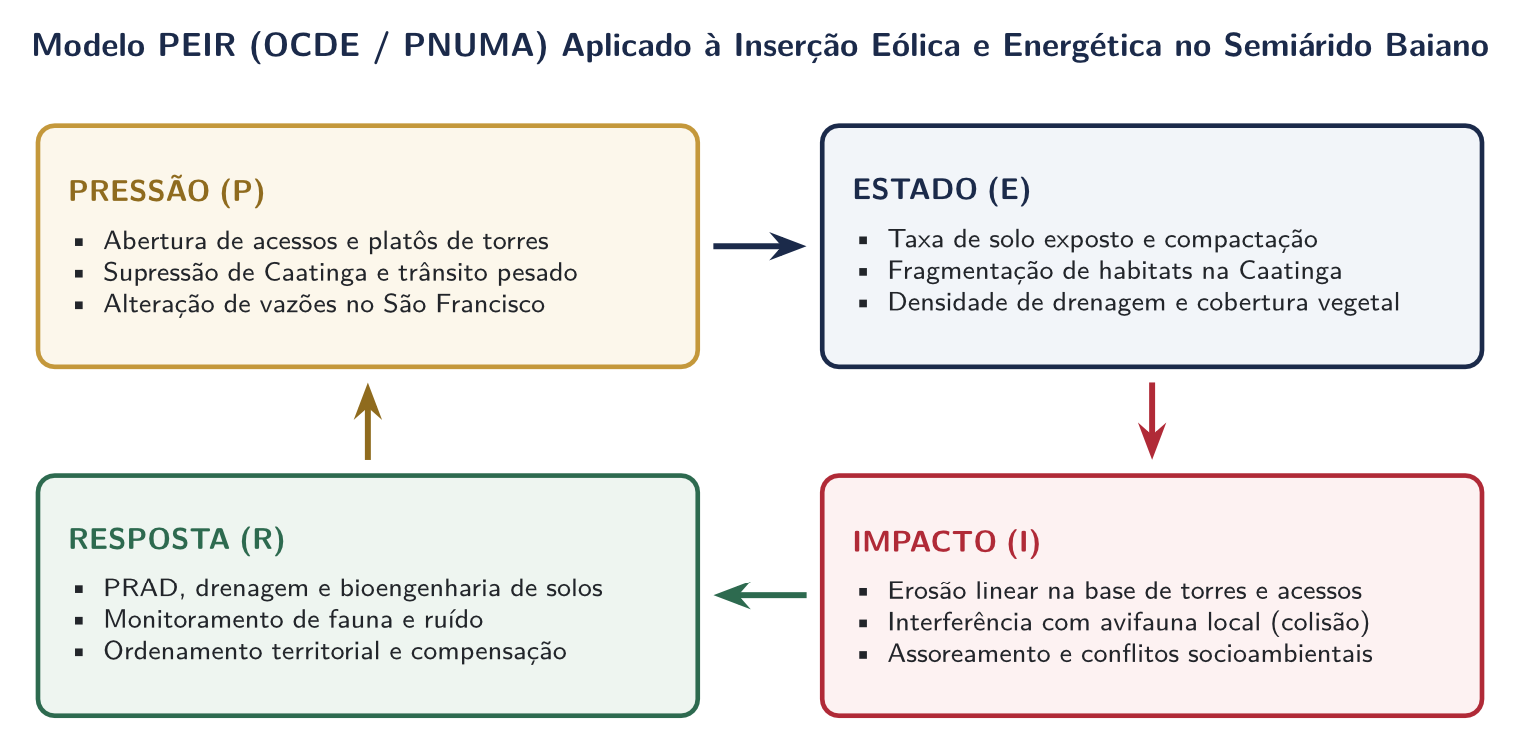
\includegraphics[keepaspectratio]{capitulos/../img/fig08_modelo_peir_semiarido.png}}

}

\caption{\label{fig-modelo_peir_semiarido}Arquitetura cíclica do modelo
PEIR aplicada à inserção eólica e energética no Semiárido Baiano,
integrando vetores de pressão, alterações de estado biofísico, impactos
socioambientais e respostas de gestão e bioengenharia.}

\end{figure}%

A leitura da Figura~\ref{fig-modelo_peir_semiarido} evidencia que o
modelo PEIR não é uma lista linear estática, mas um \textbf{ciclo de
retroalimentação}. Cada componente responde a uma pergunta específica,

A pressão representa ações que participam da transformação do ambiente,
como abertura de acessos, supressão vegetal e alteração operacional de
vazões. O estado descreve condições observáveis dos compartimentos, como
cobertura, densidade do solo e qualidade da água. A escolha do indicador
deve declarar qual dessas relações pretende acompanhar.

O impacto corresponde às consequências que a alteração produz sobre
funções ambientais e grupos sociais. A perda de capacidade de uma
captação ou o comprometimento de um habitat exige relacionar a condição
biofísica ao receptor afetado. O mesmo processo pode ser representado
por indicadores distintos quando a pergunta de análise muda, desde que a
posição adotada no modelo seja justificada.

A resposta reúne medidas de gestão e intervenção, incluindo controle de
drenagem, recuperação da cobertura, manutenção e revisão de regras
operacionais. Indicadores de execução permitem acompanhar as medidas
implantadas. Indicadores de resultado verificam a resposta do ambiente e
sustentam a revisão da intervenção.

\subsection{Métricas de campo e interpretação das
unidades}\label{muxe9tricas-de-campo-e-interpretauxe7uxe3o-das-unidades}

A taxa de supressão relaciona a área removida à área total da poligonal.
As duas áreas devem ser expressas na mesma unidade. A multiplicação da
proporção por 100 fornece seu valor percentual.

\[
T_{\mathrm{sup}} = \frac{A_{\mathrm{sup}}}{A_{\mathrm{pol}}} \times 100
\]

O símbolo \(A_{\mathrm{sup}}\) representa a área de vegetação suprimida
e \(A_{\mathrm{pol}}\) a área total de referência, ambas em hectares ou
em outra unidade comum. O resultado é informado em porcentagem. A área
de referência e a data precisam acompanhar o valor, pois sua mudança
altera a comparação.

A densidade viária divide o comprimento dos acessos pela área analisada.
Para obter quilômetros de acesso por quilômetro quadrado, a extensão
deve estar em quilômetros e a área em quilômetros quadrados.

\[
D_v = \frac{L_{\mathrm{acessos}}}{A_{\mathrm{ref}}}
\]

O comprimento total é representado por \(L_{\mathrm{acessos}}\) e a área
de referência por \(A_{\mathrm{ref}}\). A unidade do resultado é
\(\mathrm{km\,km^{-2}}\). Quando a área foi fornecida em hectares, sua
conversão utiliza a relação \(1\ \mathrm{km^2}=100\ \mathrm{ha}\). A
densidade informa a extensão relativa da rede, cuja interpretação
ambiental depende também de sua posição na drenagem e na cobertura
vegetal.

A correção simplificada da mortalidade de aves utiliza a contagem
observada e as probabilidades de detecção e persistência. O exemplo
assume busca integral da área considerada e define o período da
contagem.

\[
M_{\mathrm{est}} = \frac{N_{\mathrm{obs}}}{e\,p}
\]

O número observado de carcaças é \(N_{\mathrm{obs}}\). A eficiência da
busca é representada por \(e\) e a persistência entre campanhas por
\(p\), com valores maiores que zero e até 1. O resultado corresponde ao
período acompanhado e deve ser normalizado por torre e por tempo quando
essa for a finalidade. A fórmula é um recurso didático simplificado,
cuja utilização operacional depende do desenho e das correções
apropriadas ao levantamento.

A variação relativa de um indicador compara a diferença com seu valor
inicial. A convenção abaixo produz valores positivos para aumento e
negativos para redução.

\[
\Delta_{\%} = \frac{X_f-X_i}{X_i} \times 100
\]

Os símbolos \(X_i\) e \(X_f\) representam valores inicial e final
obtidos em condições comparáveis. O cálculo exige \(X_i\ne0\). Quando o
valor inicial é zero, a mudança deve ser descrita por diferença absoluta
e pelas condições observadas. Para indicadores já expressos em
porcentagem, a diferença entre percentuais é informada em pontos
percentuais, enquanto a divisão pela condição inicial produz uma
variação relativa.

\subsection{Estudo de Caso Integrado, Viagem de Campo no Semiárido
Baiano}\label{estudo-de-caso-integrado-viagem-de-campo-no-semiuxe1rido-baiano}

A atividade de campo prevista na Semana 11 do Plano CHF662 examina a
região de \textbf{Canudos} e o eixo energético do \textbf{Rio São
Francisco}, com referência a \textbf{Paulo Afonso, Rodelas, Sobradinho,
Casa Nova, Sento Sé e Juazeiro}. A leitura desse território relaciona a
Caatinga, as formas do relevo, os usos da água e as infraestruturas de
geração e transmissão. A observação deve registrar as condições de cada
parada, distinguindo o que foi visto, o que foi informado por documentos
e o que permanece como hipótese de análise.

\subsection{Leitura das infraestruturas durante o
campo}\label{leitura-das-infraestruturas-durante-o-campo}

Os acessos e as plataformas dos aerogeradores conectam a implantação
elétrica à dinâmica da vertente (Figura~\ref{fig-canudos-acessos}). A
superfície exposta pode receber o impacto direto das gotas, enquanto
valetas e bueiros modificam a direção e a concentração do escoamento. O
registro de campo deve localizar saídas de drenagem, proteção dos
taludes e eventuais caminhos que alcancem a rede hidrográfica. A
fotografia permite reconhecer o arranjo, enquanto a avaliação de impacto
depende de medições e de observação temporal.

\begin{figure}[H]

\centering{

\pandocbounded{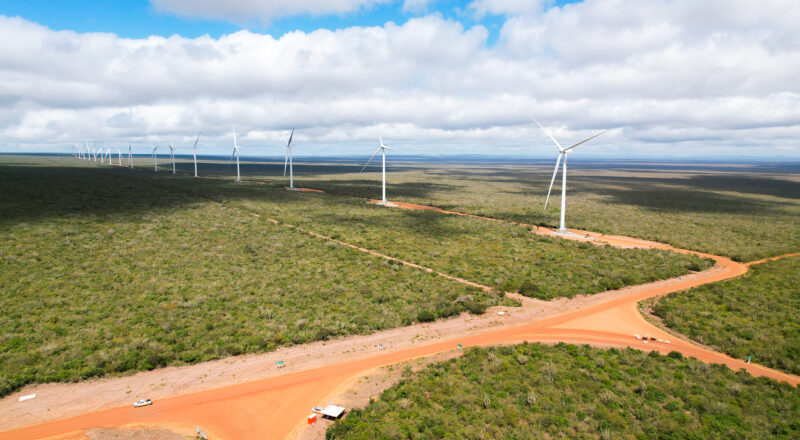
\includegraphics[keepaspectratio,alt={Vista aérea de aerogeradores interligados por acessos de solo exposto em área de Caatinga}]{capitulos/../img/canudos_aerogeradores_acessos.jpg}}

}

\caption{\label{fig-canudos-acessos}Aerogeradores, plataformas e acessos
em área de Caatinga. Fonte acervo didático disponibilizado pelo docente,
identificado como Canudos.}

\end{figure}%

A implantação linear pode atravessar unidades de drenagem e aproximar
áreas de solo exposto dos canais (Figura~\ref{fig-canudos-linear}). A
análise deve confrontar a rede de acessos com divisores, declividades e
trechos de concentração de fluxo. A proporção de área suprimida informa
a extensão da intervenção, enquanto a posição e a continuidade dos
corredores ajudam a explicar sua conexão com erosão e fragmentação.

\begin{figure}[H]

\centering{

\pandocbounded{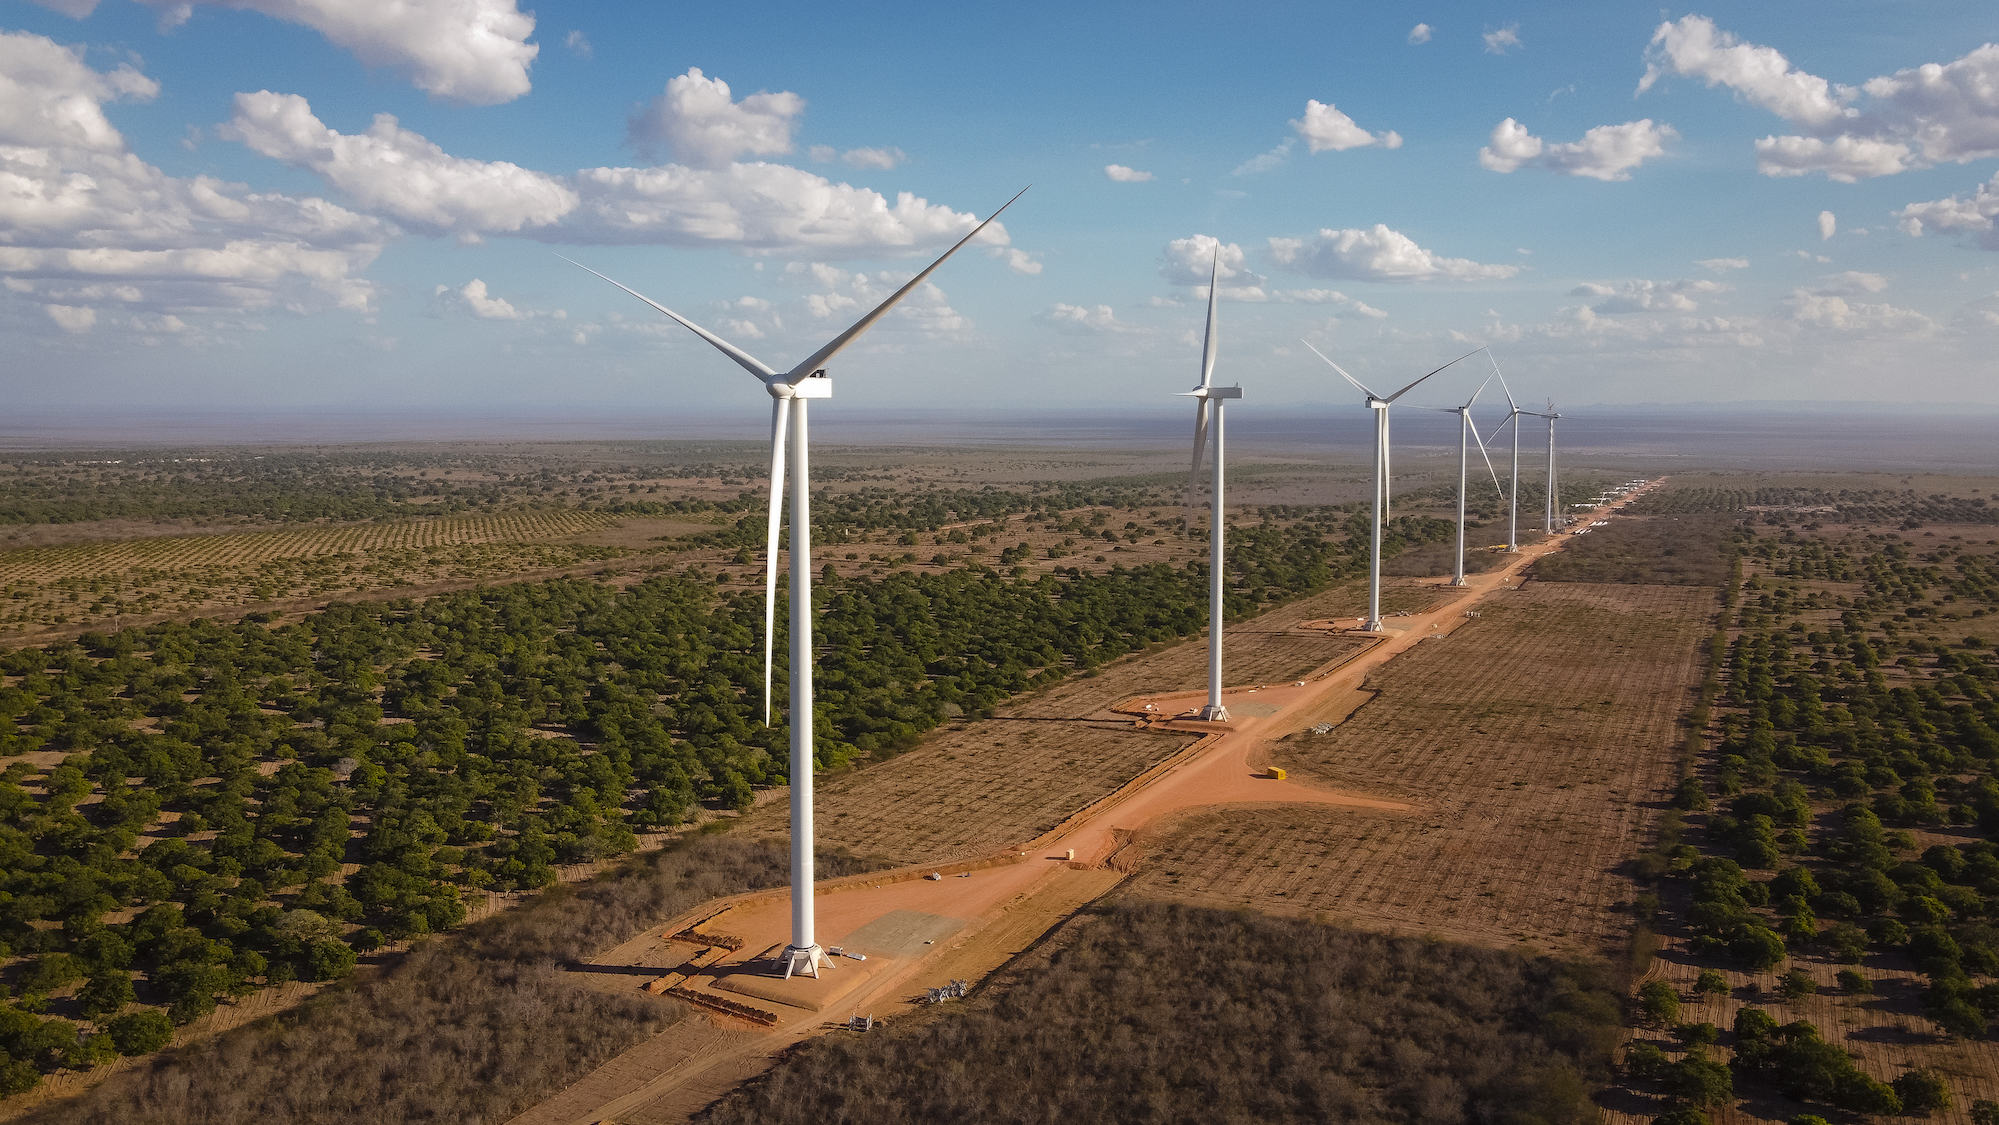
\includegraphics[keepaspectratio,alt={Aerogeradores alinhados ao longo de uma estrada sobre superfície de solo exposto}]{capitulos/../img/canudos_arranjo_linear.jpg}}

}

\caption{\label{fig-canudos-linear}Arranjo linear de aerogeradores e
acessos. Fonte acervo didático disponibilizado pelo docente,
identificado como Canudos. Enquadramento original preservado.}

\end{figure}%

O armazenamento hidrelétrico modifica o regime de circulação da água e
conecta geração a abastecimento, irrigação e manutenção de habitats
(Figura~\ref{fig-sobradinho-usina}). A observação da estrutura deve ser
acompanhada de dados de nível, vazão e operação, com referência à data.
Uma fotografia registra a condição visível de um momento e precisa ser
situada na série temporal para apoiar a interpretação do funcionamento
do reservatório.

\begin{figure}[H]

\centering{

\pandocbounded{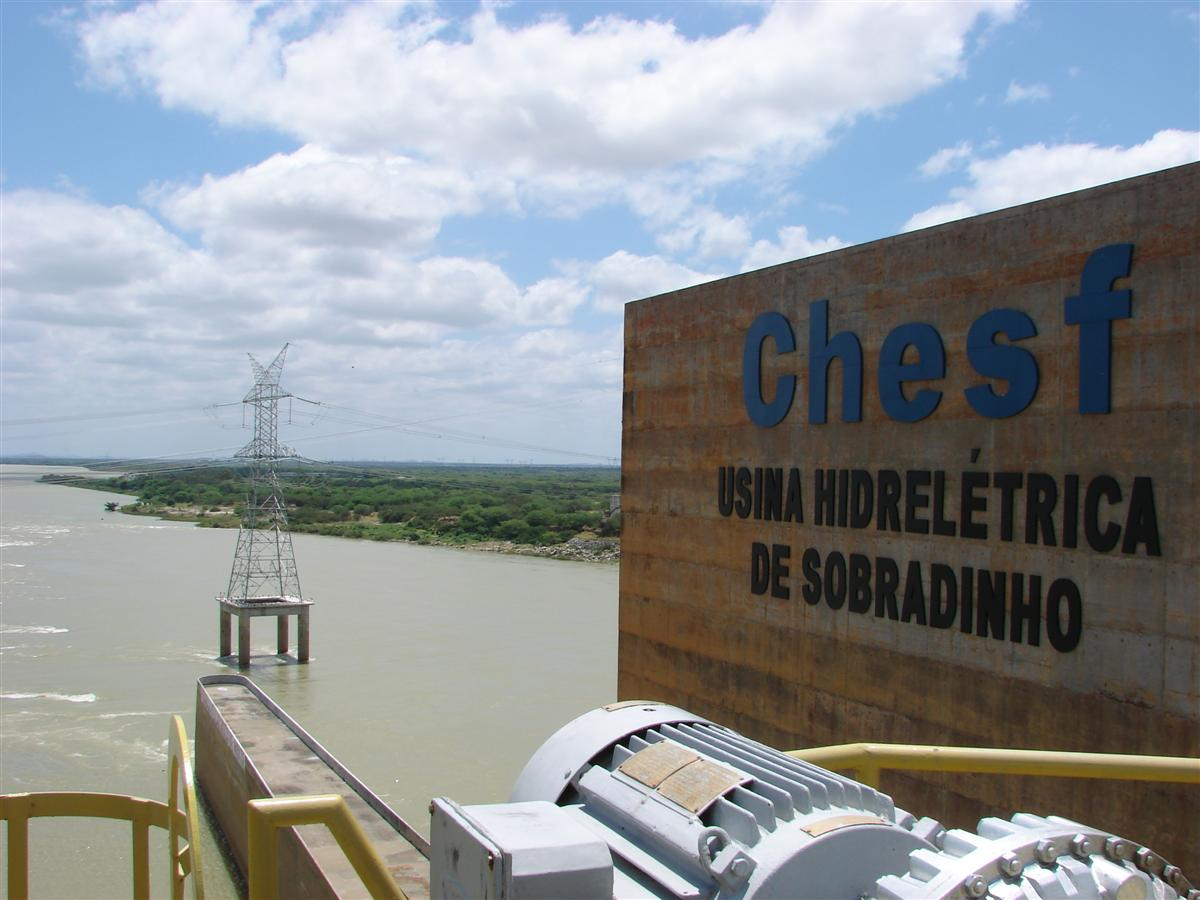
\includegraphics[keepaspectratio,alt={Vista da estrutura da Usina Hidrelétrica de Sobradinho}]{capitulos/../img/sobradinho_usina_glauco_umbelino.jpg}}

}

\caption{\label{fig-sobradinho-usina}Usina Hidrelétrica de Sobradinho,
Bahia. Fotografia de Glauco Umbelino, reproduzida sem alteração. Fonte
\href{https://commons.wikimedia.org/wiki/File:Usina_Hidreletrica_de_Sobradinho-BA.jpg}{Wikimedia
Commons}, licença \href{https://creativecommons.org/licenses/by/2.0/}{CC
BY 2.0}.}

\end{figure}%

Arranjos fotovoltaicos flutuantes acrescentam interfaces entre módulos,
flutuadores, amarrações e superfície da água
(Figura~\ref{fig-fpv-detalhe}). Variação de nível, vento e ondas
modificam as solicitações sobre o conjunto. A avaliação ambiental também
precisa considerar sombreamento, circulação da água, manutenção,
navegação e acessos, com critérios adequados à escala da implantação.

\begin{figure}[H]

\centering{

\pandocbounded{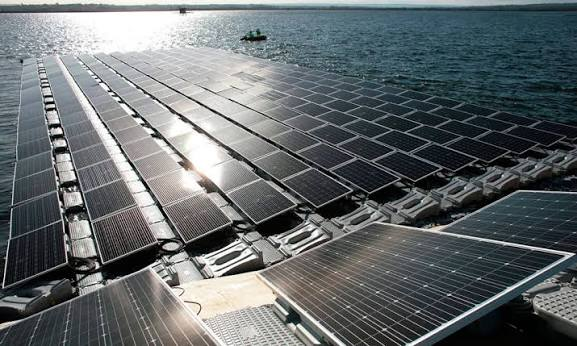
\includegraphics[keepaspectratio,alt={Módulos fotovoltaicos sobre flutuadores junto à superfície de um reservatório}]{capitulos/../img/fotovoltaica_flutuante_detalhe.jpg}}

}

\caption{\label{fig-fpv-detalhe}Detalhe de módulos fotovoltaicos
instalados em estrutura flutuante. Fonte acervo didático disponibilizado
pelo docente. Instalação sem identificação documental no material
consultado.}

\end{figure}%

A configuração do conjunto deve ser examinada junto ao espaço ocupado e
às faixas necessárias para circulação e manutenção
(Figura~\ref{fig-fpv-arranjo}). Comparações entre alternativas exigem
informar a área analisada, as restrições de uso e a condição
hidrodinâmica considerada. As fotografias fornecidas ilustram soluções
construtivas e não constituem, por si, comprovação da viabilidade de
implantação em um local específico.

\begin{figure}[H]

\centering{

\pandocbounded{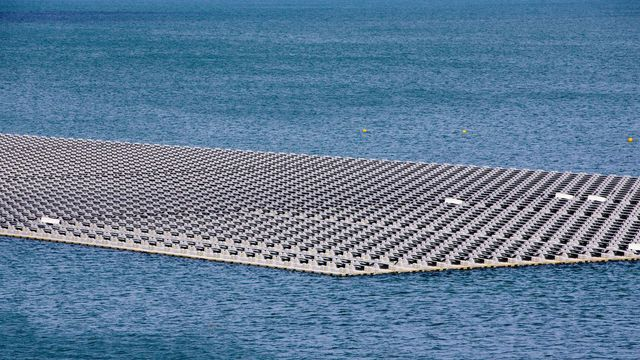
\includegraphics[keepaspectratio,alt={Conjunto de módulos solares flutuantes formando uma plataforma sobre a água}]{capitulos/../img/fotovoltaica_flutuante_arranjo.jpeg}}

}

\caption{\label{fig-fpv-arranjo}Arranjo fotovoltaico flutuante em um
corpo de água. Fonte acervo didático disponibilizado pelo docente.
Instalação sem identificação documental no material consultado.}

\end{figure}%

\subsection{Evidência publicada sobre pistas de vento e erosão em
Xingó}\label{eviduxeancia-publicada-sobre-pistas-de-vento-e-erosuxe3o-em-xinguxf3}

As pistas de vento e os focos erosivos foram examinados por Holanda e
colaboradores no artigo publicado em 2020 na \emph{Revista Brasileira de
Geografia Física} (Figura~\ref{fig-xingo-publicado-2020}). O mapa do
segmento II relaciona a geometria do reservatório à localização dos
focos identificados. Essa representação permite formular perguntas sobre
exposição das margens e direcionar o levantamento de materiais e
processos.

\begin{figure}[H]

\centering{

\pandocbounded{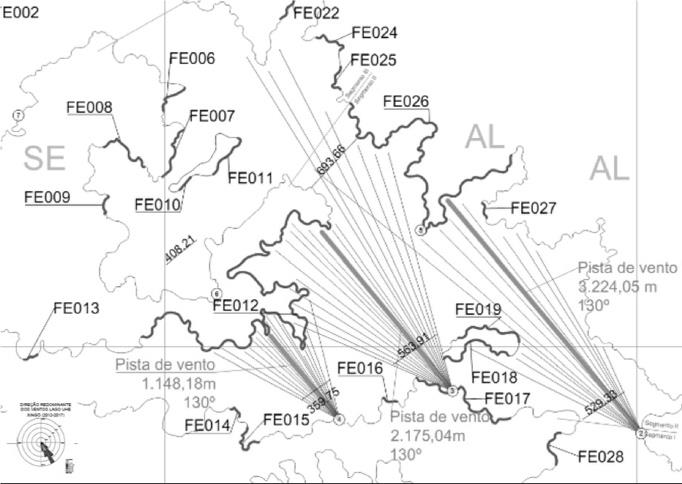
\includegraphics[keepaspectratio,alt={Mapa publicado de Xingó com três pistas de vento no segmento II e focos erosivos identificados por códigos FE}]{capitulos/../img/artigo_publicado_xingo_fetch_2020.jpeg}}

}

\caption{\label{fig-xingo-publicado-2020}Mapa de pistas de vento do
segmento II do Lago da UHE Xingó, período de 2012 a 2017. Reprodução da
Figura 7 de Holanda e colaboradores (2020), extraída do PDF editorial
sem alteração dos valores ou do enquadramento. Fonte
\href{https://doi.org/10.26848/rbgf.v13.2.p887-902}{artigo publicado},
licença \href{https://creativecommons.org/licenses/by/4.0/}{CC BY 4.0}.}

\end{figure}%

A associação espacial orienta uma hipótese sobre a ação das ondas, cuja
avaliação também depende da resistência dos materiais, da variação do
nível e de outras fontes de solicitação. A comparação com mapas de um
estudo posterior deve conferir a convenção de azimute, a definição de
fetch e a data da geometria utilizada. As representações são mantidas
com seus critérios de origem para que diferenças entre procedimentos
possam ser examinadas.

\subsection{Convergência com o estudo de ondas e seleção de sítios em
Xingó}\label{converguxeancia-com-o-estudo-de-ondas-e-seleuxe7uxe3o-de-suxedtios-em-xinguxf3}

O estudo de Santos, Holanda e Wanderley sobre ondas e fotovoltaica
flutuante em Xingó permite discutir a ligação entre geometria, vento e
escolha de sítios (Figura~\ref{fig-xingo-fetch}). O material consultado
corresponde ao manuscrito e ao conjunto de dados disponibilizados pelo
autor. Xingó é utilizado como estudo comparativo no \textbf{Baixo São
Francisco, entre Alagoas e Sergipe}, enquanto o roteiro de campo
descrito anteriormente se refere ao eixo baiano. Essa distinção situa
corretamente a comparação territorial.

\begin{figure}[H]

\centering{

\pandocbounded{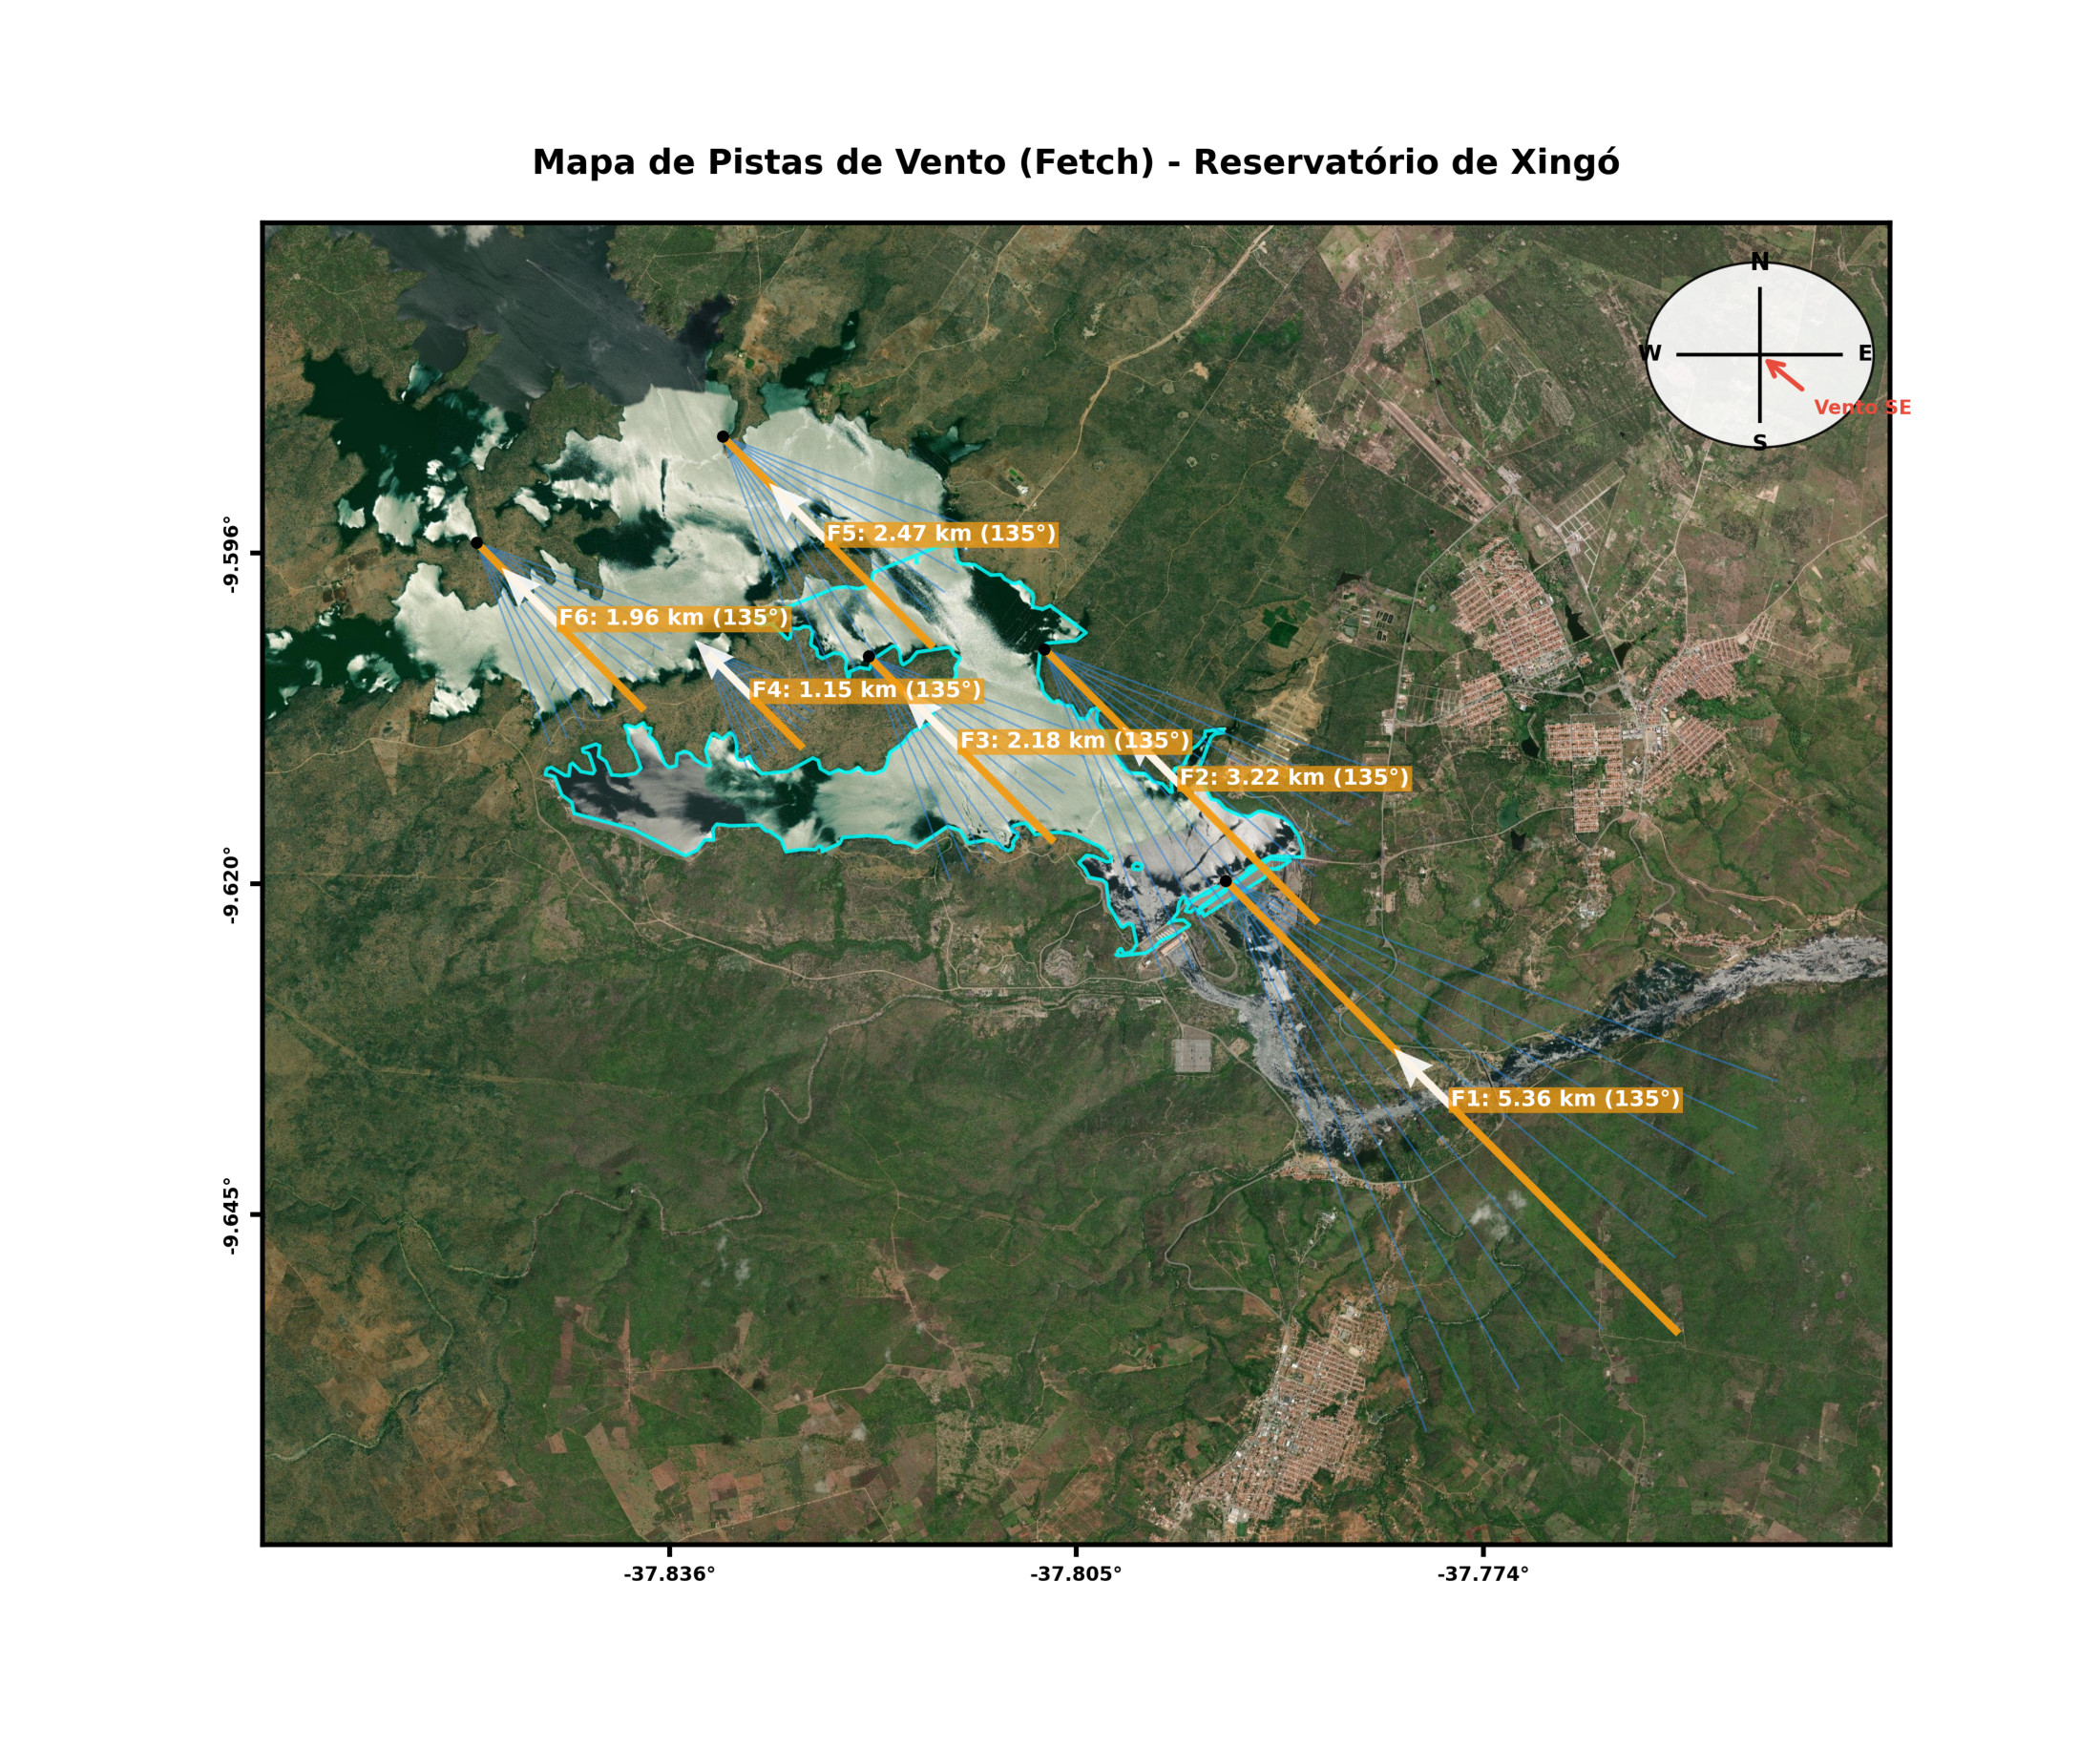
\includegraphics[keepaspectratio,alt={Mapa de Xingó com pistas de vento, orientação de sudeste e comprimentos de fetch em diferentes setores}]{capitulos/../img/artigo_xingo_fetch.jpg}}

}

\caption{\label{fig-xingo-fetch}Pistas de vento consideradas no estudo
de Xingó. Fonte Santos, Holanda e Wanderley, manuscrito sobre seleção de
sítios para fotovoltaica flutuante, figura do acervo fornecido pelo
autor. O conjunto de dados do estudo informa licença CC BY 4.0.
Reprodução da figura sem alteração dos valores ou do enquadramento.}

\end{figure}%

O fetch corresponde à distância de atuação do vento sobre a água em uma
direção considerada. Sua extensão depende da geometria do reservatório e
da posição do ponto analisado. O fetch efetivo combina pistas
direcionais segundo a formulação adotada. A altura significativa de
onda, representada por \(H_s\), pode ser observada por instrumentação ou
estimada por modelo, devendo essa origem acompanhar cada resultado.

A seleção de sítios relaciona esses resultados à batimetria e às
restrições de ocupação (Figura~\ref{fig-xingo-zoneamento}). As classes
de aptidão do mapa pertencem às condições e aos critérios do estudo de
origem. Sua aplicação em Sobradinho ou em outro reservatório exige
recalcular as variáveis com geometria, nível, vento e usos locais. A
coerência física de uma relação calculada pelo próprio modelo deve ser
distinguida da validação com medições independentes.

\begin{figure}[H]

\centering{

\pandocbounded{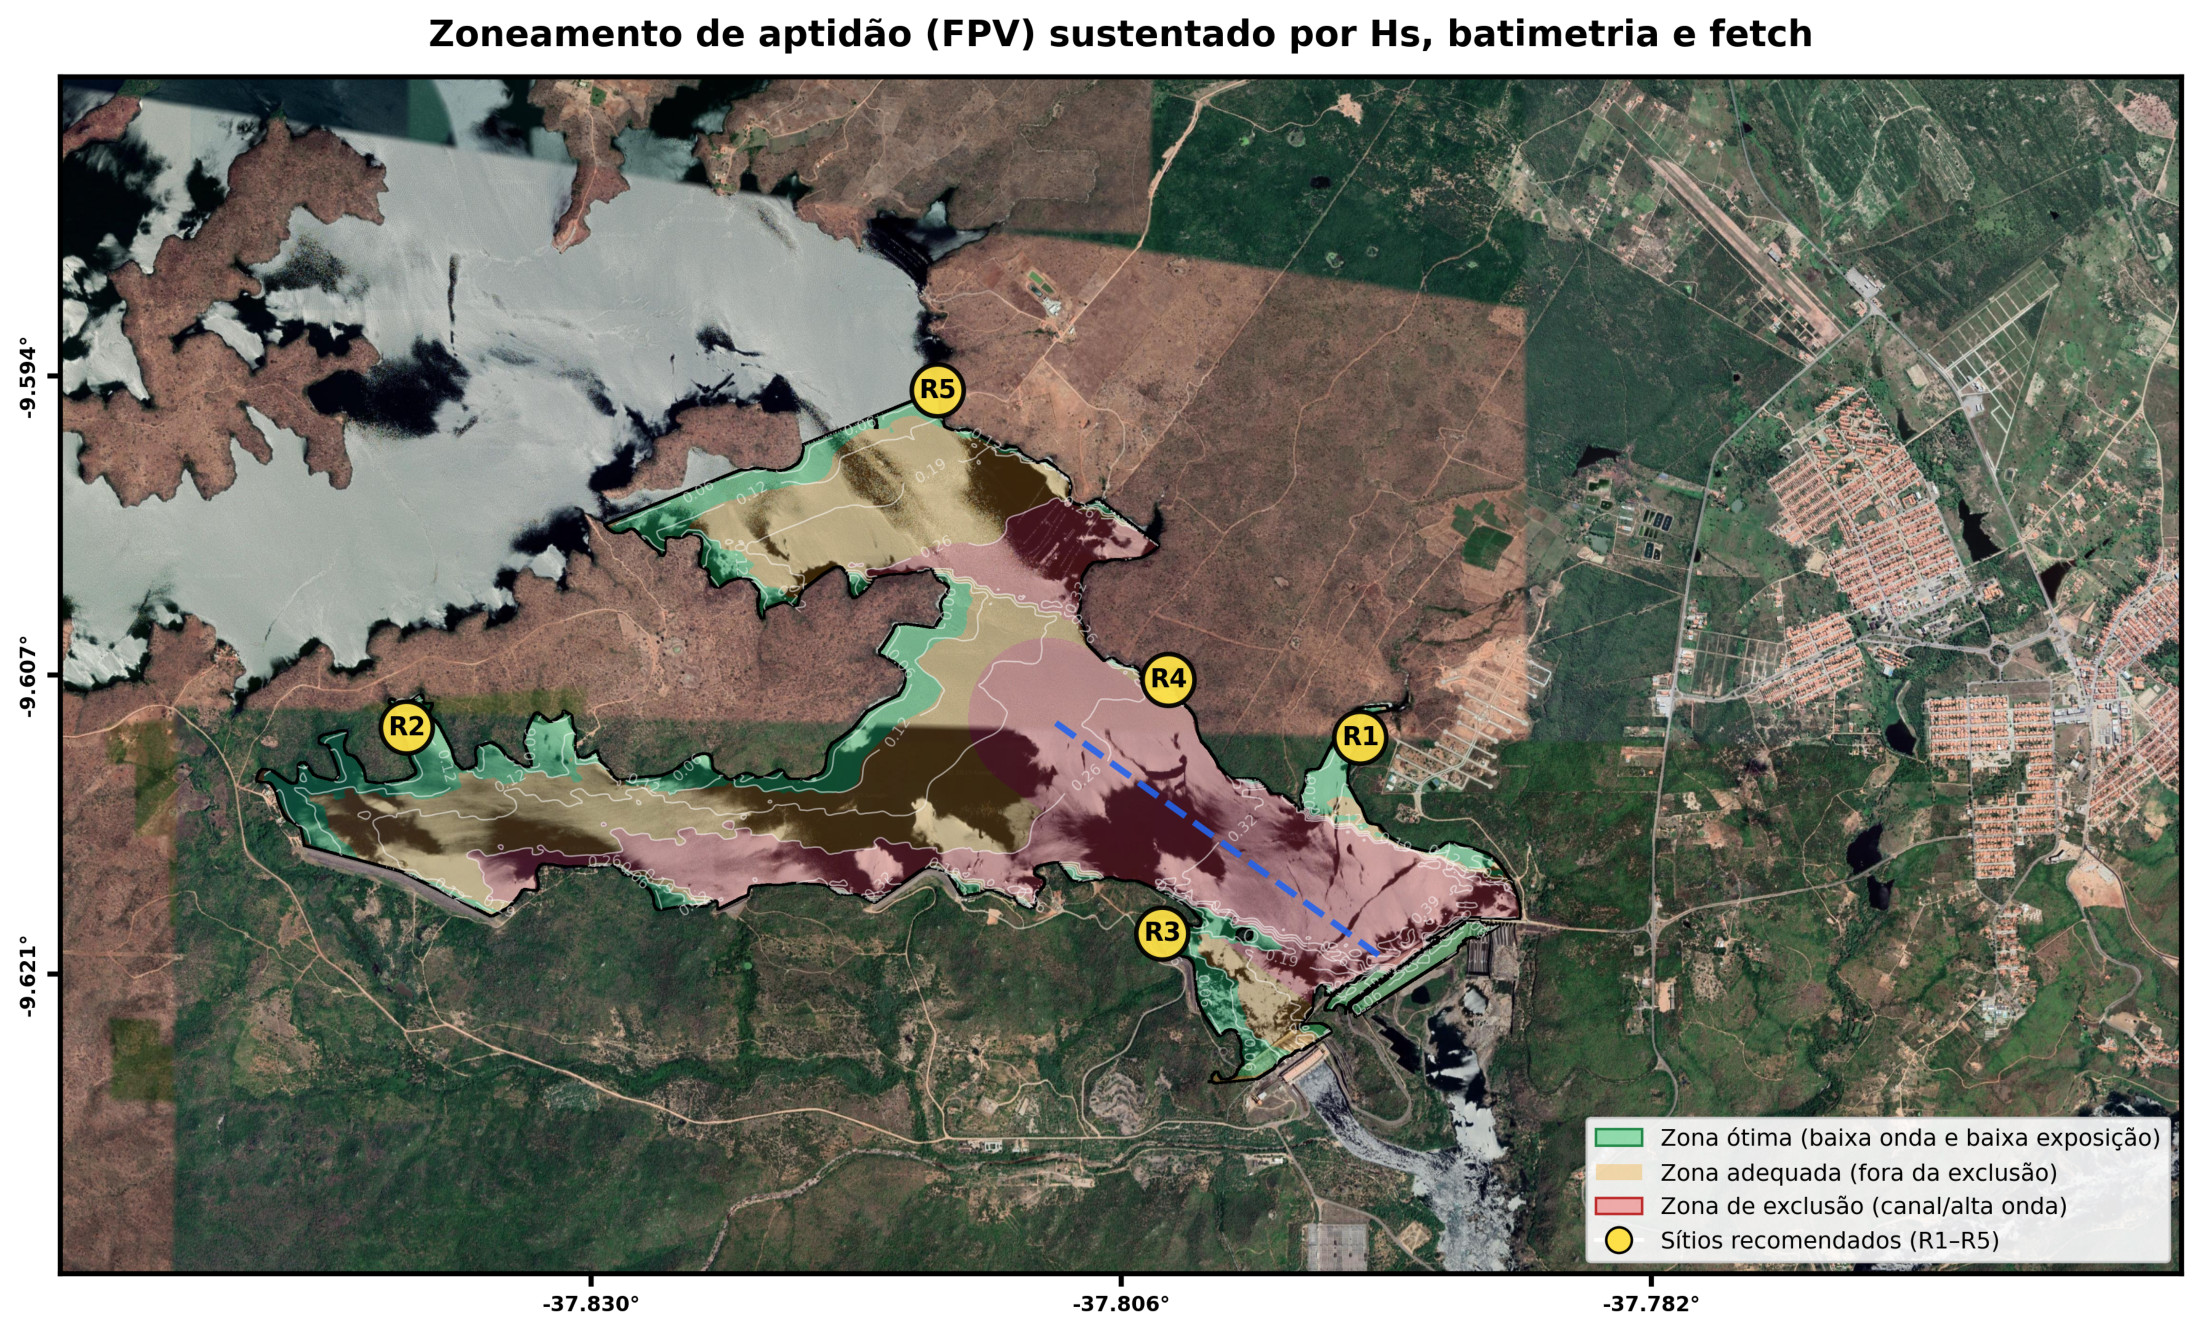
\includegraphics[keepaspectratio,alt={Mapa de zoneamento de Xingó com classes de exposição e sítios R1 a R5}]{capitulos/../img/artigo_xingo_zoneamento.jpg}}

}

\caption{\label{fig-xingo-zoneamento}Zoneamento de aptidão para
fotovoltaica flutuante no estudo de Xingó, com setores de baixa
exposição, classes intermediárias e exclusão. Fonte Santos, Holanda e
Wanderley, manuscrito e acervo de figuras fornecidos pelo autor.
Mantidos os valores e as classes do original.}

\end{figure}%

{\def\LTcaptype{none} % do not increment counter
\begin{longtable}[]{@{}
  >{\raggedright\arraybackslash}p{(\linewidth - 4\tabcolsep) * \real{0.3333}}
  >{\raggedright\arraybackslash}p{(\linewidth - 4\tabcolsep) * \real{0.3333}}
  >{\raggedright\arraybackslash}p{(\linewidth - 4\tabcolsep) * \real{0.3333}}@{}}
\toprule\noalign{}
\begin{minipage}[b]{\linewidth}\raggedright
Informação
\end{minipage} & \begin{minipage}[b]{\linewidth}\raggedright
Relação com o diagnóstico
\end{minipage} & \begin{minipage}[b]{\linewidth}\raggedright
Conferência necessária para a integração
\end{minipage} \\
\midrule\noalign{}
\endhead
\bottomrule\noalign{}
\endlastfoot
Geometria e nível do reservatório & Definem o espelho de água e
condicionam as pistas de vento. & Data, referência de nível, sistema de
coordenadas e resolução da base. \\
Velocidade e direção do vento & Descrevem a forçante utilizada na
análise de ondas. & Altura de medição, intervalo de agregação, falhas e
representatividade espacial. \\
Fetch e altura significativa de onda & Relacionam geometria e resposta
hidrodinâmica. & Formulação, hipóteses e distinção entre resultados
calculados e observados. \\
Focos erosivos e materiais das margens & Situam os receptores da ação
hidrodinâmica. & Método de levantamento, evolução temporal e resistência
dos materiais. \\
Navegação, captação e habitat & Identificam usos e funções que precisam
ser considerados na localização. & Fontes documentais, verificação em
campo e critérios de restrição. \\
\end{longtable}
}

O cruzamento entre focos de erosão, pistas de vento e margens permite
formular hipóteses sobre exposição e resposta. A associação espacial
deve ser examinada junto à variação do nível, às propriedades do
material e às ondas geradas por embarcações. No arquivo de focos
consultado, os campos de coordenadas precisam ter sua ordem e seu
sistema de referência conferidos antes do uso em SIG. Essa conferência
evita deslocar pontos e produzir convergências aparentes entre camadas
incompatíveis.

\subsubsection{Fatores Locacionais de Viabilidade da Matriz Eólica no
Semiárido}\label{fatores-locacionais-de-viabilidade-da-matriz-euxf3lica-no-semiuxe1rido}

A concentração de parques eólicos em Canudos, Casa Nova, Sento Sé e no
entorno do Lago de Sobradinho não é aleatória. Ela resulta da
convergência de quatro condicionantes geográficos e infraestruturais,

A avaliação do recurso eólico deve utilizar séries e mapas com altura,
período e método identificados. O
\href{https://www.ba.gov.br/secti/20/atlas-eolico-da-bahia}{Atlas Eólico
da Bahia} oferece uma referência institucional para examinar a
distribuição regional. A faixa de 7,5 a 9,5 metros por segundo a 100
metros de altura, utilizada como cenário de interpretação nesta
apostila, precisa ser verificada com dados do local antes de
caracterizar um empreendimento.

\textbf{Relevo de chapadas, patamares elevados e serras residuais.}
Cristas, serrotes e chapadas elevadas acima da Depressão Sertaneja
aceleram o escoamento atmosférico por efeito topográfico (efeito Venturi
e compressão de fluxo em cristas), posicionando os aerogeradores acima
da camada de maior rugosidade superficial.

\textbf{Proximidade de linhas de transmissão e subestações do SIN.} O
eixo histórico de geração hidrelétrica de Paulo Afonso (complexo CHESF)
e Sobradinho já estruturava redes de transmissão de alta tensão
conectadas ao Sistema Interligado Nacional (SIN), reduzindo custos de
escoamento da energia eólica e solar recém-implantada. \textbf{Estrutura
fundiária e baixo preço relativo da terra.} Grandes imóveis rurais e
áreas de uso comunal (como fundos de pasto) no Semiárido permitiram
contratos de arrendamento extensivos, ainda que frequentemente
acompanhados de assimetrias informacionais e conflitos territoriais.

\subsubsection{Convivência com a Caatinga e Diagnóstico dos Principais
Impactos
Ambientais}\label{convivuxeancia-com-a-caatinga-e-diagnuxf3stico-dos-principais-impactos-ambientais}

Embora a energia eólica apresente baixas emissões de gases de efeito
estufa na fase de operação, classificá-la de forma acrítica como
``energia de impacto zero'' constitui um erro metodológico grave em
Análise Ambiental. A avaliação em campo no eixo Canudos-Submédio São
Francisco demonstra que os impactos concentram-se na fase de implantação
e na reorganização territorial, exigindo diagnóstico rigoroso,

\textbf{Supressão de vegetação e fragmentação da Caatinga.} A instalação
de cada aerogerador demanda um platô nivelado para fundação e operação
de guindastes de grande porte, além de acessos largos com baixa
declividade longitudinal para transporte de pás (que ultrapassam \(60\)
a \(80\text{ m}\) de comprimento), valas de cabeamento subterrâneo,
subestações e faixas de servidão de linhas de transmissão. Ainda que a
fração suprimida aparente ser pequena em relação à poligonal total do
parque, a abertura linear de estradas fragmenta habitats, amplia o
efeito de borda e facilita a entrada de espécies invasoras, caça ilegal
e retirada de lenha.

\textbf{Erosão na base das torres, cortes de estrada e drenagem
desordenada.} Nos pedimentos e bordas de chapadas de Canudos e Sento Sé,
predominam solos rasos, arenosos ou pedregosos, com baixa coesão natural
e chuvas convectivas concentradas de alta intensidade. O terraplenamento
dos platôs e o escoamento concentrado ao longo das estradas compactadas
(sem caixas de contenção ou dissipadores adequados) desencadeiam sulcos
e ravinas na borda dos taludes, expondo fundações, soterrando vegetação
a jusante e assoreando riachos intermitentes e barreiros comunitários.

\textbf{Interferência com a avifauna e quiropterofauna local.} A região
de Canudos abriga populações críticas de aves endêmicas e ameaçadas, com
destaque emblemático para a arara-azul-de-lear (\emph{Anodorhynchus
leari}), que realiza deslocamentos diários entre áreas de dormitório em
paredões areníticos (como o Raso da Catarina e a Estação Biológica de
Canudos) e áreas de alimentação com licurizeiros (\emph{Syagrus
coronata}). A implantação de aerogeradores e linhas de transmissão em
rotas de voo implica risco de colisão, efeito barreira (desvio
energético oneroso) e perda de áreas de forrageamento, exigindo estudos
prévios de telemetria, zonas de exclusão e monitoramento sistemático.

\textbf{Regularização de vazões e conflitos por usos múltiplos da água
no Submédio São Francisco.} Ao longo do eixo Sobradinho-Casa
Nova-Juazeiro-Rodelas-Paulo Afonso, a operação em cascata das usinas
hidrelétricas alterou profundamente o pulso natural de cheias e vazantes
do Rio São Francisco. A redução de vazões defluentes em períodos de
crise hídrica acentua a salinização no baixo curso, favorece a
proliferação de bancos de areia e macrófitas, restringe a agricultura de
vazante e intensifica disputas entre geração hidrelétrica, irrigação de
fruticultura (polo Petrolina-Juazeiro), abastecimento urbano e
comunidades ribeirinhas e quilombolas.

\subsection{Roteiro Prático de Observação em Campo
(DCHF/UEFS)}\label{roteiro-pruxe1tico-de-observauxe7uxe3o-em-campo-dchfuefs}

Durante o percurso técnico em Canudos e no Submédio São Francisco, a
equipe discente deve registrar evidências georreferenciadas em quatro
eixos integrados, (i) \textbf{relevo e substrato} (posição
geomorfológica das torres, presença de solos rasos ou afloramentos,
declividade dos acessos); (ii) \textbf{processos erosivos e drenagem}
(selamento, sulcos em borda de platô, saídas de drenagem pluvial e
assoreamento de drenagens efêmeras); (iii) \textbf{cobertura da Caatinga
e fauna} (fisionomia vegetal, presença de licurizeiros, efeito de borda
e sinalização de monitoramento faunístico); e (iv) \textbf{dinâmica
hídrica e socioambiental} (nível de operação dos reservatórios, áreas de
irrigação, comunidades de fundo de pasto e percepção local sobre
benefícios e incômodos dos empreendimentos).

\subsection{Ficha do indicador e tratamento de dados
ausentes}\label{ficha-do-indicador-e-tratamento-de-dados-ausentes}

A ficha de um indicador define o fenômeno acompanhado, a forma de
cálculo e o suporte espacial. Para densidade de focos erosivos em
acessos, por exemplo, é necessário registrar o comprimento efetivamente
inspecionado, o critério de reconhecimento de um foco e o tratamento
dado às feições conectadas. A repetição da campanha exige manter esses
critérios.

Um trecho sem vistoria representa informação ausente. A atribuição de
zero a esse trecho reduziria artificialmente a densidade calculada. O
relatório deve apresentar a extensão observada e a proporção coberta
pela campanha, permitindo avaliar a representatividade do resultado. A
mesma lógica vale para falhas em sensores, imagens encobertas por nuvens
e coletas laboratoriais perdidas.

No acompanhamento de aves, a contagem de carcaças depende da área
efetivamente pesquisada, do intervalo entre buscas, da remoção por
necrófagos e da capacidade de detecção. A correção simples utilizada nos
exercícios ilustra parte dessas relações. Uma estimativa operacional
exige protocolo apropriado e avaliação das incertezas de cada
componente.

Uma resposta de gestão também precisa separar execução e desempenho.
Comprimento de drenagem construído informa execução, enquanto redução de
incisões ou manutenção da cobertura informa resultados ambientais. O
monitoramento deve acompanhar ambos, pois uma obra concluída pode exigir
manutenção ou revisão do seu funcionamento.

\section{Etapa 4 - Exemplos
resolvidos}\label{etapa-4---exemplos-resolvidos-9}

\subsection{Exemplo 10.1 - Seleção de indicadores e interpretação do
monitoramento}\label{exemplo-10.1---seleuxe7uxe3o-de-indicadores-e-interpretauxe7uxe3o-do-monitoramento}

\subsubsection{Situação e condições do
exercício}\label{situauxe7uxe3o-e-condiuxe7uxf5es-do-exercuxedcio}

Uma equipe técnica da UEFS precisa propor indicadores para acompanhar a
conservação da Caatinga no entorno de um complexo eólico em Canudos,
Bahia. O problema é reconhecer a evolução da exposição do solo e das
feições erosivas associadas a cortes, plataformas e acessos. O
monitoramento deve permitir comparar campanhas e identificar onde uma
medida de drenagem ou revegetação precisa ser revista.

Quatro candidatos foram apresentados. O quadro registra sua formulação
inicial, que precisa ser examinada antes de aceitar o indicador.

{\def\LTcaptype{none} % do not increment counter
\begin{longtable}[]{@{}
  >{\raggedright\arraybackslash}p{(\linewidth - 4\tabcolsep) * \real{0.3333}}
  >{\raggedright\arraybackslash}p{(\linewidth - 4\tabcolsep) * \real{0.3333}}
  >{\raggedright\arraybackslash}p{(\linewidth - 4\tabcolsep) * \real{0.3333}}@{}}
\toprule\noalign{}
\begin{minipage}[b]{\linewidth}\raggedright
Candidato
\end{minipage} & \begin{minipage}[b]{\linewidth}\raggedright
Informação proposta
\end{minipage} & \begin{minipage}[b]{\linewidth}\raggedright
Condição do levantamento
\end{minipage} \\
\midrule\noalign{}
\endhead
\bottomrule\noalign{}
\endlastfoot
I & Percentual de área com solo exposto em cortes e plataformas. &
Imagens comparáveis, poligonal definida e critério de classificação
conferido em campo. \\
II & Percepção genérica de beleza da paisagem. & Opiniões registradas
sem questionário padronizado ou desenho amostral. \\
III & Densidade de focos erosivos ativos por quilômetro de acesso. &
Vistoria georreferenciada em trechos fixos e ficha de reconhecimento das
feições. \\
IV & Sequenciamento genômico semanal de todos os micro-organismos do
solo em 80 pontos. & Programa sem protocolo que traduza os resultados em
decisão sobre o problema acompanhado. \\
\end{longtable}
}

Os dados numéricos apresentados a seguir são \textbf{hipotéticos e
destinados ao exercício}. A equipe dispõe de R\$ 8.000 por campanha. O
levantamento de imagens e a vistoria conjunta custam R\$ 5.000 por
campanha, enquanto a proposta laboratorial foi estimada em R\$ 80.000
por rodada semanal. Esses valores ilustram uma restrição de orçamento e
não representam preços de mercado.

\subsubsection{Entendimento dos critérios de
seleção}\label{entendimento-dos-crituxe9rios-de-seleuxe7uxe3o}

A relevância expressa a relação entre a informação e a decisão de
gestão. Um indicador de solo exposto é relevante porque permite
acompanhar a proteção superficial da área analisada. A solidez analítica
depende de um procedimento capaz de produzir valores comparáveis, com
definição de área, feição e forma de medição.

A mensurabilidade envolve acesso aos dados, custo e capacidade de
repetir o levantamento durante o período necessário. A sensibilidade
corresponde à capacidade de registrar alterações do fenômeno em um
intervalo útil. Um protocolo pode ser executável e, ainda assim, exigir
outro calendário para detectar a resposta esperada.

Nesta triagem, a letra \textbf{A} indica atendimento nas condições
descritas, \textbf{P} indica atendimento parcial e \textbf{N} indica
ausência de uma condição necessária. As letras representam julgamentos
fundamentados. A decisão utiliza a justificativa de cada critério, sem
converter automaticamente essas categorias em uma soma de pontos.

\subsubsection{Aplicação dos critérios aos
candidatos}\label{aplicauxe7uxe3o-dos-crituxe9rios-aos-candidatos}

O candidato I responde ao problema de proteção superficial e possui uma
unidade de comparação definida. A classificação de solo exposto exige
manter a mesma poligonal e um protocolo consistente entre imagens. A
verificação em campo deve distinguir superfície mineral descoberta,
cobertura vegetal seca e sombra, pois confusões entre essas classes
alteram o resultado. Com essas condições atendidas, o indicador pode
registrar a evolução após a revegetação.

O candidato II aborda uma dimensão social pertinente, mas sua formulação
atual reúne opiniões produzidas em condições diferentes. A percepção da
paisagem pode ser investigada com pergunta definida, amostra justificada
e procedimento de aplicação. A reformulação permitiria estudar essa
dimensão de maneira comparável e complementar o monitoramento físico.

O candidato III relaciona feições ativas ao comprimento efetivamente
observado. A ficha deve definir o reconhecimento de um foco, a forma de
registrar feições conectadas e os sinais utilizados para reconhecer
atividade. A repetição nos mesmos trechos permite comparar campanhas,
especialmente quando as condições de chuva e manutenção são
documentadas.

O candidato IV ultrapassa o orçamento informado e não apresenta uma
ligação operacional entre os resultados e a decisão acompanhada. O
estudo da comunidade microbiana pode ser pertinente a outras perguntas e
escalas de pesquisa. Para esta proposta, a frequência, o número de
pontos e a finalidade analítica precisariam ser reformulados.

{\def\LTcaptype{none} % do not increment counter
\begin{longtable}[]{@{}
  >{\raggedright\arraybackslash}p{(\linewidth - 10\tabcolsep) * \real{0.1364}}
  >{\centering\arraybackslash}p{(\linewidth - 10\tabcolsep) * \real{0.1818}}
  >{\centering\arraybackslash}p{(\linewidth - 10\tabcolsep) * \real{0.1818}}
  >{\centering\arraybackslash}p{(\linewidth - 10\tabcolsep) * \real{0.1818}}
  >{\centering\arraybackslash}p{(\linewidth - 10\tabcolsep) * \real{0.1818}}
  >{\raggedright\arraybackslash}p{(\linewidth - 10\tabcolsep) * \real{0.1364}}@{}}
\toprule\noalign{}
\begin{minipage}[b]{\linewidth}\raggedright
Candidato
\end{minipage} & \begin{minipage}[b]{\linewidth}\centering
Relevância
\end{minipage} & \begin{minipage}[b]{\linewidth}\centering
Solidez analítica
\end{minipage} & \begin{minipage}[b]{\linewidth}\centering
Mensurabilidade
\end{minipage} & \begin{minipage}[b]{\linewidth}\centering
Sensibilidade
\end{minipage} & \begin{minipage}[b]{\linewidth}\raggedright
Decisão justificada
\end{minipage} \\
\midrule\noalign{}
\endhead
\bottomrule\noalign{}
\endlastfoot
I & A & A & A & A & Selecionar com classificação e verificação
padronizadas. \\
II & P & N & N & P & Reformular o protocolo antes da utilização. \\
III & A & A & A & A & Selecionar com trechos fixos e definição de foco
ativo. \\
IV & P & P & N & P & Reformular o programa e sua relação com a
decisão. \\
\end{longtable}
}

\subsubsection{Cálculo do percentual de solo
exposto}\label{cuxe1lculo-do-percentual-de-solo-exposto}

Na campanha inicial, a poligonal de cortes e plataformas mede 12,0 ha,
dos quais 3,6 ha foram classificados como solo exposto. A área de
referência é a poligonal efetivamente acompanhada. O numerador e o
denominador devem utilizar a mesma unidade.

\[
T_{\mathrm{exp}} = \frac{A_{\mathrm{exp}}}{A_{\mathrm{ref}}} \times 100
\]

O símbolo \(A_{\mathrm{exp}}\) representa a área com solo exposto e
\(A_{\mathrm{ref}}\) a área total de referência. A divisão produz uma
proporção adimensional e a multiplicação por 100 expressa o resultado em
porcentagem.

\[
T_{\mathrm{exp},1} = \frac{3{,}6\ \mathrm{ha}}{12{,}0\ \mathrm{ha}} \times 100 = 30{,}0\%
\]

O resultado informa que 30,0\% da poligonal acompanhada apresentava solo
exposto. A área medida deve permanecer disponível junto à porcentagem,
pois ela permite verificar o cálculo e comparar a magnitude absoluta da
exposição.

\subsubsection{Cálculo da densidade de focos
erosivos}\label{cuxe1lculo-da-densidade-de-focos-erosivos}

A vistoria inicial cobriu 6,0 km de acessos e identificou 18 focos
ativos segundo o protocolo do exercício. A densidade relaciona o número
observado ao comprimento inspecionado.

\[
D_{\mathrm{eros}} = \frac{N_{\mathrm{focos}}}{L_{\mathrm{vist}}}
\]

O símbolo \(N_{\mathrm{focos}}\) representa a contagem de focos ativos e
\(L_{\mathrm{vist}}\) o comprimento de acesso efetivamente vistoriado.
Trechos sem inspeção precisam ser registrados como informação ausente.

\[
D_{\mathrm{eros},1} = \frac{18\ \mathrm{focos}}{6{,}0\ \mathrm{km}} = 3{,}0\ \mathrm{focos\,km^{-1}}
\]

Essa densidade descreve a frequência espacial das feições reconhecidas.
A gravidade precisa ser avaliada com informações complementares, como
dimensões, atividade, conexão com canais e elementos expostos a jusante.

\subsubsection{Comparação após a
intervenção}\label{comparauxe7uxe3o-apuxf3s-a-intervenuxe7uxe3o}

Após ações de drenagem e revegetação, a segunda campanha encontrou 2,4
ha de solo exposto na mesma poligonal de 12,0 ha. A vistoria percorreu
novamente os 6,0 km e registrou 9 focos ativos. Os métodos e critérios
foram mantidos.

\[
T_{\mathrm{exp},2} = \frac{2{,}4}{12{,}0} \times 100 = 20{,}0\%
\]

\[
D_{\mathrm{eros},2} = \frac{9}{6{,}0} = 1{,}5\ \mathrm{focos\,km^{-1}}
\]

A exposição diminuiu de 30,0\% para 20,0\%, correspondendo a uma redução
de \textbf{10,0 pontos percentuais}. A redução relativa utiliza o valor
inicial como referência.

\[
r_{\mathrm{exp}} = \frac{30{,}0 - 20{,}0}{30{,}0} \times 100 \approx 33{,}3\%
\]

A densidade passou de 3,0 para 1,5 focos por quilômetro. Mantido o mesmo
suporte espacial, a redução relativa corresponde a 50,0\%.

\[
r_{\mathrm{eros}} = \frac{3{,}0 - 1{,}5}{3{,}0} \times 100 = 50{,}0\%
\]

\subsubsection{Interpretação e conferência da
resposta}\label{interpretauxe7uxe3o-e-conferuxeancia-da-resposta}

Os resultados indicam melhora dos indicadores nas condições observadas.
A interpretação deve considerar a chuva entre campanhas, a sazonalidade
da vegetação, a manutenção e a possibilidade de mudança no comportamento
dos focos remanescentes. Uma redução na contagem pode coexistir com
aumento de tamanho de determinadas feições, o que justifica manter
registros de dimensões e fotografias em posições repetidas.

A conclusão do exercício seleciona os candidatos I e III para o
monitoramento proposto, recomenda reformular II e IV e relaciona cada
decisão aos critérios. O relatório mantém os valores medidos, o suporte
espacial e o método de cálculo. Os resultados posteriores à intervenção
sustentam a comparação temporal, cuja atribuição causal exige examinar
as condições ambientais e operacionais do período.

\subsection{Atividade 10.1A - Seleção e cálculo para resolução
autônoma}\label{atividade-10.1a---seleuxe7uxe3o-e-cuxe1lculo-para-resoluuxe7uxe3o-autuxf4noma}

Uma equipe precisa acompanhar a recuperação de acessos de outro
empreendimento no Semiárido. O programa dispõe de R\$ 6.000 por campanha
e prevê medições antes e depois das intervenções. Todos os valores desta
atividade são didáticos.

{\def\LTcaptype{none} % do not increment counter
\begin{longtable}[]{@{}
  >{\raggedright\arraybackslash}p{(\linewidth - 4\tabcolsep) * \real{0.3333}}
  >{\raggedright\arraybackslash}p{(\linewidth - 4\tabcolsep) * \real{0.3333}}
  >{\raggedright\arraybackslash}p{(\linewidth - 4\tabcolsep) * \real{0.3333}}@{}}
\toprule\noalign{}
\begin{minipage}[b]{\linewidth}\raggedright
Candidato
\end{minipage} & \begin{minipage}[b]{\linewidth}\raggedright
Proposta de monitoramento
\end{minipage} & \begin{minipage}[b]{\linewidth}\raggedright
Informação sobre o protocolo
\end{minipage} \\
\midrule\noalign{}
\endhead
\bottomrule\noalign{}
\endlastfoot
A & Percentual de solo exposto em uma poligonal fixa. & Imagens
comparáveis e verificação em campo; custo conjunto com a vistoria de R\$
4.500 por campanha. \\
B & Satisfação dos moradores com os acessos e a drenagem. & Questionário
padronizado, amostra justificada e aplicação nas mesmas comunidades. \\
C & Densidade de focos erosivos ativos por quilômetro. & Trechos fixos,
ficha georreferenciada e definição prévia de atividade da feição. \\
D & Análise laboratorial diária de todos os atributos químicos do solo
em 100 pontos. & Custo estimado de R\$ 48.000 por rodada e ausência de
justificativa para a frequência diária. \\
\end{longtable}
}

{\def\LTcaptype{none} % do not increment counter
\begin{longtable}[]{@{}lrr@{}}
\toprule\noalign{}
Dado observado & Campanha inicial & Campanha posterior \\
\midrule\noalign{}
\endhead
\bottomrule\noalign{}
\endlastfoot
Área total da poligonal acompanhada & 9,0 ha & 9,0 ha \\
Área classificada como solo exposto & 1,80 ha & 1,08 ha \\
Comprimento efetivamente vistoriado & 4,8 km & 4,8 km \\
Focos erosivos ativos & 12 & 7 \\
\end{longtable}
}

Construa uma matriz de triagem com os quatro critérios utilizados no
exemplo resolvido. Justifique as classificações e as decisões
considerando as condições fornecidas, inclusive a possibilidade de
acompanhar dimensões sociais com um protocolo adequado.

Calcule a taxa de solo exposto e a densidade de focos em cada campanha.
Apresente a fórmula, a substituição, as unidades e a interpretação.
Determine a mudança da taxa em pontos percentuais e a redução relativa
de cada indicador, mantendo precisão durante o cálculo e arredondando os
resultados finais de maneira informada.

Redija uma interpretação técnica que relacione a comparação às condições
de chuva, manutenção e representatividade do levantamento. Indique quais
dados adicionais permitiriam examinar se as feições remanescentes
aumentaram de tamanho. A atividade deve ser entregue com seu próprio
desenvolvimento e não apresenta gabarito nesta apostila.

\subsection{Exemplo 10.2 (Intermediário). Cálculo de Supressão Vegetal e
Densidade Viária em Parque
Eólico}\label{exemplo-10.2-intermediuxe1rio.-cuxe1lculo-de-supressuxe3o-vegetal-e-densidade-viuxe1ria-em-parque-euxf3lico}

\textbf{Situação analisada.} Durante a análise do Estudo de Impacto
Ambiental (EIA) de um parque eólico situado em uma chapada no eixo
Canudos-Sento Sé, você precisa quantificar dois indicadores de Pressão,
a taxa percentual de supressão da Caatinga e a densidade de acessos
internos dentro da poligonal do empreendimento.

\textbf{Dados disponíveis.} Área total da poligonal do empreendimento,
\(A_{\text{pol}} = 1.600\text{ ha}\). Número de aerogeradores, \(25\)
torres, cada qual exigindo um platô de montagem de \(0{,}45\text{ ha}\).
Rede de estradas internas de acesso, extensão total
\(L_{\text{acessos}} = 18{,}0\text{ km}\) com largura média da faixa
suprimida de \(10\text{ m}\). Área conjunta de subestação e canteiro de
obras, \(2{,}75\text{ ha}\).

\textbf{Problema a resolver.} Calcular (a) a área total suprimida
\(A_{\text{sup}}\) em hectares; (b) a taxa percentual de supressão
\(T_{\text{sup}}\); e (c) a densidade viária interna \(D_v\) em
\(\text{km}\cdot\text{km}^{-2}\).

\textbf{Fundamento da análise.} Conversão homogênea de unidades métricas
para hectares (\(1\text{ ha} = 10.000\text{ m}^2\)) e quilômetros
quadrados (\(1\text{ km}^2 = 100\text{ ha}\)), seguida da aplicação das
fórmulas de \(T_{\text{sup}}\) e \(D_v\).

\textbf{Desenvolvimento.} \textbf{Etapa 1, Área dos platôs das torres,}

\[
A_{\text{platôs}} = 25 \times 0{,}45\text{ ha} = 11{,}25\text{ ha}
\]

\textbf{Etapa 2, Área das estradas de acesso.} Convertemos
\(18{,}0\text{ km}\) para metros (\(18.000\text{ m}\)), multiplicamos
pela largura de \(10\text{ m}\) e dividimos por
\(10.000\text{ m}^2\cdot\text{ha}^{-1}\),

\[
A_{\text{acessos}} = \frac{18.000\text{ m} \times 10\text{ m}}{10.000\text{ m}^2\cdot\text{ha}^{-1}} = \frac{180.000}{10.000} = 18{,}00\text{ ha}
\]

\textbf{Etapa 3, Área total suprimida e taxa percentual,}

\[
A_{\text{sup}} = 11{,}25 + 18{,}00 + 2{,}75 = 32{,}00\text{ ha}
\]

\[
T_{\text{sup}} = \frac{32{,}00}{1.600} \times 100\% = 0{,}02 \times 100\% = 2{,}00\%
\]

\textbf{Etapa 4, Densidade viária interna.} Convertemos a área da
poligonal para \(\text{km}^2\),
\(A_{\text{km}^2} = 1.600 / 100 = 16{,}0\text{ km}^2\).

\[
D_v = \frac{18{,}0\text{ km}}{16{,}0\text{ km}^2} = 1{,}125\text{ km}\cdot\text{km}^{-2}
\]

\textbf{Interpretação do resultado.} Área total suprimida de
\(32{,}00\text{ ha}\), equivalente a uma taxa de supressão de
\(2{,}00\%\) da poligonal, e densidade viária interna de
\(1{,}125\text{ km}\cdot\text{km}^{-2}\).

\textbf{Condições de validade.} Note um ponto crítico de interpretação
geográfica, embora \(2{,}00\%\) pareça um percentual reduzido em termos
de área absoluta, a maior parcela da supressão (\(18{,}0\text{ ha}\), ou
\(56{,}25\%\) do total) corresponde a corredores lineares (estradas),
gerando uma densidade viária superior a
\(1\text{ km}\cdot\text{km}^{-2}\). Esse arranjo linear potencializa a
fragmentação da Caatinga e a concentração de escoamento pluvial.

\subsection{Exemplo 10.3 (Intermediário). Construção de Matriz PEIR para
o Eixo Energético do Submédio São
Francisco}\label{exemplo-10.3-intermediuxe1rio.-construuxe7uxe3o-de-matriz-peir-para-o-eixo-energuxe9tico-do-submuxe9dio-suxe3o-francisco}

\textbf{Situação analisada.} A partir das observações da viagem de campo
entre Sobradinho, Casa Nova, Juazeiro, Rodelas e Paulo Afonso, estruture
uma matriz PEIR que integre simultaneamente dois vetores territoriais
presentes nesse eixo, (1) implantação de complexos eólicos em bordas de
chapada e (2) regularização hidrelétrica de vazões no Rio São Francisco.

\textbf{Dados disponíveis.} Roteiro de campo DCHF/UEFS e evidências
registradas em reservatórios, calha fluvial e parques eólicos instalados
sobre Caatinga hiperxerófila.

\textbf{Problema a resolver.} Preencher uma matriz PEIR coerente
contendo Pressão, Estado, Impacto e Resposta com indicadores mensuráveis
para cada vetor.

\textbf{Fundamento da análise.} Separação rigorosa entre atividade
antrópica (P), alteração física ou biótica do compartimento (E),
consequência socioambiental (I) e instrumento de gestão ou mitigação
(R).

\textbf{Desenvolvimento.} Organizamos os vínculos causais na tabela
padronizada abaixo,

{\def\LTcaptype{none} % do not increment counter
\begin{longtable}[]{@{}
  >{\raggedright\arraybackslash}p{(\linewidth - 8\tabcolsep) * \real{0.2000}}
  >{\raggedright\arraybackslash}p{(\linewidth - 8\tabcolsep) * \real{0.2000}}
  >{\raggedright\arraybackslash}p{(\linewidth - 8\tabcolsep) * \real{0.2000}}
  >{\raggedright\arraybackslash}p{(\linewidth - 8\tabcolsep) * \real{0.2000}}
  >{\raggedright\arraybackslash}p{(\linewidth - 8\tabcolsep) * \real{0.2000}}@{}}
\toprule\noalign{}
\begin{minipage}[b]{\linewidth}\raggedright
\textbf{Vetor}
\end{minipage} & \begin{minipage}[b]{\linewidth}\raggedright
\textbf{Pressão (P)}
\end{minipage} & \begin{minipage}[b]{\linewidth}\raggedright
\textbf{Estado (E)}
\end{minipage} & \begin{minipage}[b]{\linewidth}\raggedright
\textbf{Impacto (I)}
\end{minipage} & \begin{minipage}[b]{\linewidth}\raggedright
\textbf{Resposta (R)}
\end{minipage} \\
\midrule\noalign{}
\endhead
\bottomrule\noalign{}
\endlastfoot
\textbf{Eólicas na Caatinga} & Abertura de acessos e platôs
(\(\text{ha}\) suprimidos; \(D_v\) em \(\text{km}\cdot\text{km}^{-2}\)).
& Solo exposto (\(\%\)), compactação (\(D_s\)) e fragmentação vegetal. &
Erosão na base de torres (focos/km) e colisão de avifauna
(aves/torre/ano). & Drenagem pluvial, PRAD/bioengenharia e zonas de
exclusão para rotas de aves. \\
\textbf{Hidrelétricas (São Francisco)} & Operação de reservatórios com
redução de vazão defluente (\(\text{m}^3\cdot\text{s}^{-1}\)). &
Alteração do pulso hidrológico, redução de lâmina d'água e bancos
arenosos. & Perda de agricultura de vazante, conflitos com irrigação e
degradação ripária. & Alocação negociada no CBHSF, vazão ecológica
mínima e recomposição de APPs. \\
\end{longtable}
}

\textbf{Interpretação do resultado.} A matriz PEIR articulada permite
acompanhar separadamente as causas (P), as mudanças mensuráveis do meio
(E), os danos ecológicos e sociais (I) e a efetividade das ações
corretivas (R) nos dois eixos energéticos.

\textbf{Condições de validade.} Cada coluna apresenta grandezas
verificáveis e evita a confusão frequente de classificar uma atividade
(pressão) como impacto ou um programa de monitoramento (resposta) como
estado ambiental.

\subsection{Exemplo 10.4 (Avançado). Indicador Corrigido de Mortalidade
de Avifauna em Parque
Eólico}\label{exemplo-10.4-avanuxe7ado.-indicador-corrigido-de-mortalidade-de-avifauna-em-parque-euxf3lico}

\textbf{Situação analisada.} O monitoramento de avifauna em um parque
eólico com \(40\) aerogeradores próximo a corredores ecológicos da
Caatinga baiana registrou, ao longo de 12 meses de vistorias
padronizadas sob as torres, \(18\) carcaças de aves associadas à
colisão. Testes experimentais de controle de campo indicaram que a
equipe encontra em média \(60\%\) das carcaças presentes
(\(e = 0{,}60\)) e que \(75\%\) das carcaças permanecem no terreno até o
momento da vistoria sem serem removidas por animais necrófagos
(\(p = 0{,}75\)).

\textbf{Dados disponíveis.} \(N_{\text{obs}} = 18\) aves/ano; número de
torres monitoradas \(N_t = 40\); eficiência de busca \(e = 0{,}60\);
taxa de persistência de carcaças \(p = 0{,}75\). Limiar operacional de
alerta adotado no condicionante ambiental,
\(0{,}80\text{ ave}\cdot\text{torre}^{-1}\cdot\text{ano}^{-1}\).

\textbf{Problema a resolver.} Calcular (a) a taxa bruta não corrigida
por torre; (b) a mortalidade anual estimada corrigida
\(M_{\text{est}}\); e (c) a taxa corrigida por torre/ano, comparando-a
ao limiar de alerta.

\textbf{Fundamento da análise.} Aplicação do fator de correção amostral
\(M_{\text{est}} = N_{\text{obs}} / (e \cdot p)\) e relativização pelo
número de aerogeradores.

\textbf{Desenvolvimento.} \textbf{Etapa 1, Taxa bruta (sem correção de
viés de detecção),}

\[
T_{\text{bruta}} = \frac{18}{40} = 0{,}45\text{ ave}\cdot\text{torre}^{-1}\cdot\text{ano}^{-1}
\]

\textbf{Etapa 2, Produto dos fatores de detecção,}

\[
e \cdot p = 0{,}60 \times 0{,}75 = 0{,}45
\]

Isso significa que apenas \(45\%\) das colisões reais são efetivamente
detectadas nas buscas de campo.

\textbf{Etapa 3, Mortalidade total corrigida e taxa por torre,}

\[
M_{\text{est}} = \frac{18}{0{,}45} = 40{,}0\text{ aves}\cdot\text{ano}^{-1}
\]

\[
T_{\text{corr}} = \frac{40{,}0}{40} = 1{,}00\text{ ave}\cdot\text{torre}^{-1}\cdot\text{ano}^{-1}
\]

\textbf{Etapa 4, Comparação com o limiar de alerta
(\(0{,}80\text{ ave}\cdot\text{torre}^{-1}\cdot\text{ano}^{-1}\)),} Como
\(1{,}00 > 0{,}80\), o limiar de alerta foi ultrapassado em \(25\%\)
(\(\frac{1{,}00 - 0{,}80}{0{,}80}\times 100\% = 25\%\)).

\textbf{Interpretação do resultado.} A taxa bruta era de
\(0{,}45\text{ ave}\cdot\text{torre}^{-1}\cdot\text{ano}^{-1}\), mas a
taxa corrigida atinge
\(1{,}00\text{ ave}\cdot\text{torre}^{-1}\cdot\text{ano}^{-1}\)
(\(M_{\text{est}} = 40\) aves/ano), superando o limiar de alerta e
exigindo resposta mitigadora imediata.

\textbf{Condições de validade.} O exemplo ilustra por que relatórios sem
correção de eficiência de busca e remoção por necrófagos subestimam
impactos reais, pela taxa bruta (\(0{,}45\)), o parque pareceria abaixo
do limiar de alerta, ocultando um risco significativo à avifauna da
Caatinga.

\subsection{Exemplo 10.5 (Avançado). Avaliação Quantitativa de Eficácia
de Resposta Mitigadora no Ciclo
PEIR}\label{exemplo-10.5-avanuxe7ado.-avaliauxe7uxe3o-quantitativa-de-eficuxe1cia-de-resposta-mitigadora-no-ciclo-peir}

\textbf{Situação analisada.} Após vistoria de campo apontar erosão
acelerada nos acessos de um complexo eólico no Semiárido, o empreendedor
executou um programa de resposta (R) combinando canaletas revestidas,
dissipadores de energia em pedra rachão, paliçadas permeáveis e
semeadura de espécies nativas da Caatinga nos taludes. Antes das obras,
havia \(36\) focos erosivos ativos ao longo de \(12\text{ km}\) de
estradas e cobertura vegetal média nos taludes de \(15\%\). Doze meses
após as intervenções, nova vistoria registrou \(9\) focos ativos e
cobertura vegetal média de \(69\%\).

\textbf{Dados disponíveis.} Antes, \(F_0 = 36\) focos em
\(12\text{ km}\); cobertura \(C_0 = 15\%\). Depois (12 meses),
\(F_1 = 9\) focos em \(12\text{ km}\); cobertura \(C_1 = 69\%\). Meta
contratual do PRAD, redução mínima de \(70\%\) nos focos erosivos e
incremento mínimo de \(50\) pontos percentuais na cobertura vegetal.

\textbf{Problema a resolver.} Calcular a densidade inicial e final de
focos erosivos, a redução percentual dos focos, o ganho absoluto (pontos
percentuais) e relativo na cobertura vegetal, verificando o cumprimento
das metas.

\textbf{Fundamento da análise.} Cálculo das razões por quilômetro de
acesso e das variações absoluta e percentual entre os tempos \(t_0\) e
\(t_1\).

\textbf{Desenvolvimento.} \textbf{Etapa 1, Densidade de focos erosivos
por quilômetro de acesso,}

\[
D_{f,0} = \frac{36}{12} = 3{,}00\text{ focos}\cdot\text{km}^{-1} \qquad \text{e} \qquad D_{f,1} = \frac{9}{12} = 0{,}75\text{ foco}\cdot\text{km}^{-1}
\]

\textbf{Etapa 2, Redução percentual dos focos erosivos,}

\[
\Delta F_{\%} = \frac{9 - 36}{36} \times 100\% = \frac{-27}{36} \times 100\% = -75{,}0\% \quad (\text{redução de } 75{,}0\%)
\]

\textbf{Etapa 3, Ganho de cobertura vegetal (pontos percentuais e
aumento relativo),}

\[
\Delta C_{\text{pp}} = 69\% - 15\% = +54\text{ pontos percentuais (p.p.)}
\]

\[
\Delta C_{\text{rel}} = \frac{69 - 15}{15} \times 100\% = \frac{54}{15} \times 100\% = +360{,}0\%
\]

\textbf{Etapa 4, Conferência frente às metas do PRAD,} Redução de focos,
\(75{,}0\% \ge 70\%\) (meta cumprida). Ganho de cobertura,
\(54\text{ p.p.} \ge 50\text{ p.p.}\) (meta cumprida).

\textbf{Interpretação do resultado.} A densidade de focos caiu de
\(3{,}00\) para \(0{,}75\text{ foco}\cdot\text{km}^{-1}\) (redução de
\(75{,}0\%\)) e a cobertura vegetal avançou \(+54\) pontos percentuais
(\(+360{,}0\%\) relativos), cumprindo ambas as metas do PRAD.

\textbf{Condições de validade.} Distinguir \emph{pontos percentuais}
(diferença direta entre duas taxas, \(69\% - 15\% = 54\text{ p.p.}\)) de
\emph{variação relativa} (\(+360\%\)) evita ambiguidades graves em
relatórios de auditoria ambiental. Além disso, a permanência de \(9\)
focos ativos indica necessidade de manutenção pontual no segundo ano.

\section{Etapa 5 - Erros de
interpretação}\label{etapa-5---erros-de-interpretauxe7uxe3o-9}

\subsection{Erro 1, Confundir Dado Bruto, Pressão e Impacto na Matriz
PEIR}\label{erro-1-confundir-dado-bruto-pressuxe3o-e-impacto-na-matriz-peir}

\textbf{Equívoco frequente,} Listar ``abertura de \(18\text{ km}\) de
estradas'' na coluna de Impacto (I) ou registrar ``execução de PRAD'' na
coluna de Estado (E).

\textbf{Correção técnica,} A abertura de estradas é a ação humana
geradora de perturbação, logo pertence à \textbf{Pressão (P)}. A
execução do PRAD é uma intervenção corretiva da sociedade, portanto é
\textbf{Resposta (R)}. O \textbf{Estado (E)} retrata a condição
biofísica resultante (percentual de solo exposto), enquanto o
\textbf{Impacto (I)} expressa o dano ou consequência (ravinamento em
taludes, perda de biodiversidade, assoreamento).

\subsection{Erro 2, Assumir que Energia Eólica Equivale a Impacto
Ambiental
Nulo}\label{erro-2-assumir-que-energia-euxf3lica-equivale-a-impacto-ambiental-nulo}

\textbf{Equívoco frequente,} Afirmar em diagnósticos que parques eólicos
na Caatinga não causam degradação por serem fontes renováveis de baixa
emissão de carbono.

\textbf{Correção técnica,} Toda fonte energética possui pegada
territorial. No Semiárido Baiano, a implantação eólica envolve
terraplenagem pesada, supressão linear da Caatinga, erosão em solos
rasos de chapadas, riscos à avifauna (como a arara-azul-de-lear em
Canudos) e conflitos fundiários e sonoros que exigem licenciamento
rigoroso e monitoramento contínuo.

\subsection{Erro 3, Subestimar a Fragmentação ao Olhar Apenas o
Percentual Total de
Supressão}\label{erro-3-subestimar-a-fragmentauxe7uxe3o-ao-olhar-apenas-o-percentual-total-de-supressuxe3o}

\textbf{Equívoco frequente,} Concluir que uma taxa de supressão de
\(2\%\) em um parque eólico é ecologicamente irrelevante.

\textbf{Correção técnica,} Um pequeno percentual distribuído em forma de
malha viária extensa e linhas de transmissão cria centenas de metros de
borda exposta, interrompe o deslocamento de fauna terrestre e concentra
o escoamento superficial das chuvas torrenciais do Semiárido. Por isso,
deve-se sempre complementar \(T_{\text{sup}}\) com métricas espaciais
como a densidade viária (\(D_v\)) e o índice de fragmentação.

\subsection{Erro 4, Comparar Contagens Brutas de Fauna ou Erosão sem
Padronização
Amostral}\label{erro-4-comparar-contagens-brutas-de-fauna-ou-erosuxe3o-sem-padronizauxe7uxe3o-amostral}

\textbf{Equívoco frequente,} Relatar apenas o número absoluto de
carcaças de aves ou focos erosivos sem considerar esforço amostral,
número de torres, extensão vistoriada ou eficiência de detecção.

\textbf{Correção técnica,} Sem relativização (por torre/ano ou por km de
estrada) e sem correção de viés de detecção (\(e \cdot p\) no
monitoramento faunístico), os números não são comparáveis entre
campanhas nem entre empreendimentos, comprometendo a solidez analítica
exigida pela OCDE (2003).

\section{Etapa 6 - Exercícios de
fixação}\label{etapa-6---exercuxedcios-de-fixauxe7uxe3o-9}

\subsubsection{Nível Básico (Conceitos, Critérios e Modelo
PEIR)}\label{nuxedvel-buxe1sico-conceitos-crituxe9rios-e-modelo-peir}

\begin{enumerate}
\def\labelenumi{\arabic{enumi}.}
\item
  Explique, com um exemplo concreto ligado ao Semiárido Baiano, a
  diferença entre \textbf{dado bruto}, \textbf{indicador ambiental} e
  \textbf{índice ambiental}.
\item
  Cite os quatro critérios principais de seleção de indicadores
  ambientais propostos por OECD (2003), Fidalgo (2003) e IBGE (2018),
  explicando o risco técnico de ignorar o critério da
  \emph{mensurabilidade}.
\item
  Qual é a principal diferença conceitual entre o modelo \textbf{PER}
  (OCDE) e o modelo \textbf{PEIR} (PNUMA/GEO)? Por que essa distinção
  favorece a articulação com a Avaliação de Impacto Ambiental?
\item
  Classifique cada item abaixo como \textbf{Pressão (P)}, \textbf{Estado
  (E)}, \textbf{Impacto (I)} ou \textbf{Resposta (R)} em um parque
  eólico na Caatinga, (a) abertura de \(14\text{ km}\) de estradas de
  acesso; (b) ravina ativa de \(1{,}8\text{ m}\) de profundidade na
  saída de bueiro; (c) percentual de solo exposto de \(42\%\) no talude;
  (d) instalação de dissipadores de energia e revegetação com espécies
  nativas.
\item
  Liste três fatores locacionais geográficos que explicam a intensa
  concentração de parques eólicos na região de Canudos e no eixo do
  Submédio São Francisco (Casa Nova, Sento Sé e entorno de Sobradinho).
\end{enumerate}

\subsubsection{Nível Intermediário (Cálculos de Monitoramento e
Interpretação
Regional)}\label{nuxedvel-intermediuxe1rio-cuxe1lculos-de-monitoramento-e-interpretauxe7uxe3o-regional}

\begin{enumerate}
\def\labelenumi{\arabic{enumi}.}
\setcounter{enumi}{5}
\item
  Um projeto eólico em uma poligonal de \(1.200\text{ ha}\) na Bahia
  prevê \(30\) aerogeradores com platôs de \(0{,}40\text{ ha}\) cada,
  \(12\text{ km}\) de acessos internos com \(8\text{ m}\) de largura
  média e \(2{,}4\text{ ha}\) destinados à subestação. Calcule a área
  total suprimida (\(A_{\text{sup}}\)) e a taxa percentual de supressão
  (\(T_{\text{sup}}\)).
\item
  Em um período de estiagem prolongada no Submédio São Francisco, a
  vazão defluente média da Usina Hidrelétrica de Sobradinho foi reduzida
  de \(1.300\text{ m}^3\cdot\text{s}^{-1}\) para
  \(800\text{ m}^3\cdot\text{s}^{-1}\). Calcule a variação percentual
  dessa vazão e cite dois impactos socioambientais diretos dessa redução
  ao longo do eixo Juazeiro-Rodelas-Paulo Afonso.
\item
  No monitoramento anual de avifauna de um complexo eólico com \(50\)
  torres, registraram-se \(24\) carcaças de aves. Ensaios de campo
  indicaram eficiência de busca \(e = 0{,}80\) e persistência de
  carcaças \(p = 0{,}60\). Calcule a mortalidade total estimada
  (\(M_{\text{est}}\)) e a taxa corrigida de mortalidade em aves por
  torre por ano.
\item
  Uma poligonal de empreendimento energético abrange \(1.500\text{ ha}\)
  e contém \(27\text{ km}\) de estradas internas não pavimentadas.
  Determine a densidade viária interna (\(D_v\)) em
  \(\text{km}\cdot\text{km}^{-2}\) e discuta como esse indicador se
  relaciona com a erosão linear na Caatinga.
\item
  Após obras de drenagem superficial e bioengenharia nos taludes de um
  parque eólico, o número de focos erosivos ativos reduziu-se de \(28\)
  para \(7\) em um ano. Calcule a redução percentual obtida e
  classifique esse indicador dentro do modelo PEIR.
\end{enumerate}

\subsubsection{Nível Aplicado (Questões Objetivas
A-E)}\label{10-indicadores-ambientais-peir-nuxedvel-aplicado-questuxf5es-objetivas-ae}

\begin{enumerate}
\def\labelenumi{\arabic{enumi}.}
\setcounter{enumi}{10}
\item
  Sobre os critérios de seleção de indicadores ambientais (OECD, 2003;
  IBGE, 2018), assinale a alternativa correta,

  \begin{enumerate}
  \def\labelenumii{(\Alph{enumii})}
  \item
    Um indicador de alta qualidade deve dispensar qualquer protocolo
    padronizado, permitindo interpretações subjetivas de cada analista.
  \item
    A sensibilidade indica a capacidade do indicador de detectar
    mudanças ambientais precoces e responder às medidas de manejo em
    prazo útil.
  \item
    Indicadores compostos (índices) sempre substituem integralmente os
    indicadores individuais, tornando desnecessário reportar as
    variáveis de origem.
  \item
    A relevância técnica exige que o indicador utilize equipamentos
    laboratoriais de alto custo, independentemente da viabilidade de
    monitoramento contínuo.
  \item
    A mensurabilidade refere-se exclusivamente à possibilidade de
    converter variáveis qualitativas em médias aritméticas sem base
    amostral.
  \end{enumerate}
\item
  Na matriz PEIR aplicada ao eixo energético do Submédio São Francisco,
  a ``implantação de um programa de monitoramento telemétrico da
  arara-azul-de-lear e readequação do traçado de linhas de transmissão''
  corresponde ao componente,

  \begin{enumerate}
  \def\labelenumii{(\Alph{enumii})}
  \item
    Pressão (P), pois altera o cronograma financeiro do empreendimento.
  \item
    Estado (E), pois descreve a abundância natural da espécie na
    Caatinga.
  \item
    Impacto (I), pois representa o dano causado pelas torres ao habitat.
  \item
    Resposta (R), pois consiste em ação técnica e de gestão destinada a
    prevenir ou mitigar impactos sobre a fauna.
  \item
    Fator abiótico de base, externo ao ciclo PEIR.
  \end{enumerate}
\item
  Um parque eólico localizado em área de \(2.000\text{ ha}\) suprimiu
  \(0{,}50\text{ ha}\) por platô em \(20\) torres e abriu
  \(15\text{ km}\) de acessos com \(10\text{ m}\) de largura. Sem outras
  áreas suprimidas, a taxa percentual de supressão (\(T_{\text{sup}}\))
  da poligonal é igual a,

  \begin{enumerate}
  \def\labelenumii{(\Alph{enumii})}
  \item
    \(0{,}50\%\).
  \item
    \(0{,}75\%\).
  \item
    \(1{,}25\%\).
  \item
    \(2{,}50\%\).
  \item
    \(5{,}00\%\).
  \end{enumerate}
\item
  Em relação aos processos físicos observados em parques eólicos
  implantados em chapadas e serras residuais do Semiárido Baiano, é
  correto afirmar que,

  \begin{enumerate}
  \def\labelenumii{(\Alph{enumii})}
  \item
    A baixa pluviosidade anual do Semiárido impede completamente a
    ocorrência de erosão hídrica linear na base das torres.
  \item
    O terraplenamento de platôs e o escoamento concentrado em estradas
    compactadas sobre solos rasos potencializam sulcos, ravinas e
    assoreamento de drenagens intermitentes.
  \item
    A substituição da Caatinga por solo exposto em taludes de corte
    reduz a energia cinética do escoamento superficial.
  \item
    A instalação de aerogeradores elimina a necessidade de medidas de
    drenagem pluvial e PRAD por se tratar de energia renovável.
  \item
    Os ventos alísios de sudeste são os únicos responsáveis pelo
    transporte de sedimentos grosseiros nos bueiros das estradas de
    acesso.
  \end{enumerate}
\item
  Em um programa de monitoramento de colisão de avifauna com \(25\)
  torres eólicas durante um ano, foram encontradas \(15\) carcaças.
  Sabendo que a eficiência de busca foi \(e = 0{,}50\) e a persistência
  de carcaças foi \(p = 0{,}60\), a taxa anual corrigida de mortalidade
  por torre é,

  \begin{enumerate}
  \def\labelenumii{(\Alph{enumii})}
  \item
    \(0{,}60\text{ ave}\cdot\text{torre}^{-1}\cdot\text{ano}^{-1}\).
  \item
    \(1{,}20\text{ aves}\cdot\text{torre}^{-1}\cdot\text{ano}^{-1}\).
  \item
    \(1{,}50\text{ aves}\cdot\text{torre}^{-1}\cdot\text{ano}^{-1}\).
  \item
    \(2{,}00\text{ aves}\cdot\text{torre}^{-1}\cdot\text{ano}^{-1}\).
  \item
    \(2{,}50\text{ aves}\cdot\text{torre}^{-1}\cdot\text{ano}^{-1}\).
  \end{enumerate}
\end{enumerate}

\section{Etapa 7 - Questões de
aplicação}\label{etapa-7---questuxf5es-de-aplicauxe7uxe3o-9}

\subsection{Foco de Provas, ENADE e Concursos (IBAMA /
INEMA)}\label{foco-de-provas-enade-e-concursos-ibama-inema}

Exames de Geografia e concursos para Analista Ambiental frequentemente
combinam leitura crítica de matrizes PEIR com dilemas concretos da
transição energética no Nordeste brasileiro. Evite respostas binárias
(``energia limpa = sem impacto'' ou ``toda obra é inviável'') e
demonstre domínio da diferenciação entre Pressão, Estado, Impacto e
Resposta com métricas verificáveis.

\begin{enumerate}
\def\labelenumi{\arabic{enumi}.}
\setcounter{enumi}{15}
\item
  \textbf{{[}Questão Autoral, Estilo ENADE / Geografia{]}} A expansão da
  energia eólica no Semiárido Baiano, especialmente em municípios como
  Canudos, Sento Sé e Casa Nova, tem ampliado a participação de fontes
  renováveis na matriz elétrica nacional. Contudo, levantamentos de
  campo apontam conflitos socioambientais envolvendo fragmentação da
  Caatinga, erosão em estradas de acesso, ruído próximo a comunidades
  rurais e risco de colisão para espécies ameaçadas como a
  arara-azul-de-lear (\emph{Anodorhynchus leari}). À luz da Análise
  Ambiental integrada, avalie as afirmações a seguir,

  \begin{itemize}
  \item
    A viabilidade climática da energia eólica não dispensa o
    planejamento locacional em escala regional para evitar corredores
    ecológicos críticos e áreas de uso comunal.
  \item
    O modelo PEIR permite distinguir claramente a abertura de acessos
    (Pressão), a exposição do solo (Estado), o ravinamento em taludes
    (Impacto) e as obras de drenagem e PRAD (Resposta).
  \item
    Como a área diretamente ocupada pelas fundações das torres
    representa pequena fração do terreno, a fragmentação gerada pela
    malha viária não altera a conectividade da Caatinga.
  \end{itemize}

  É correto o que se afirma em,

  \begin{enumerate}
  \def\labelenumii{(\Alph{enumii})}
  \item
    I, apenas.
  \item
    III, apenas.
  \item
    I e II, apenas.
  \item
    II e III, apenas.
  \item
    I, II e III.
  \end{enumerate}
\item
  \textbf{{[}Questão Autoral, Estilo Concurso Analista Ambiental /
  INEMA-BA{]}} No Submédio São Francisco (trecho
  Sobradinho-Juazeiro-Rodelas-Paulo Afonso), a gestão ambiental enfrenta
  pressões simultâneas decorrentes da regularização de vazões
  hidrelétricas, da captação para perímetros irrigados e da expansão de
  infraestrutura energética. Para compor um painel estadual de
  monitoramento baseado no modelo PEIR, um técnico deve escolher o
  conjunto mais coerente de indicadores. Assinale a alternativa em que
  os quatro elementos correspondem, respectivamente, a \textbf{Pressão,
  Estado, Impacto e Resposta},

  \begin{enumerate}
  \def\labelenumii{(\Alph{enumii})}
  \item
    Assoreamento de bancos de areia; vazão defluente reduzida; plano de
    bacia; perda de área de vazante.
  \item
    Volume captado para irrigação e operação de barramentos; nível
    fluviométrico e percentual de vegetação ripária; conflito por usos
    múltiplos da água e redução da pesca artesanal; alocação negociada
    de água no comitê de bacia e recomposição de APPs.
  \item
    Recomposição de APPs; conflito por uso da água; operação de
    barramentos; nível fluviométrico.
  \item
    Nível fluviométrico; volume captado para irrigação; recomposição de
    APPs; redução da pesca artesanal.
  \item
    Conflito por uso da água; plano de bacia; volume captado; percentual
    de vegetação ripária.
  \end{enumerate}
\item
  \textbf{{[}Questão Autoral, Estilo Concurso Analista Ambiental /
  IBAMA{]}} Um órgão licenciador exigiu que um empreendimento eólico
  substituísse indicadores genéricos de seu Programa de Monitoramento
  por variáveis aderentes aos critérios da OCDE (2003). Qual proposta
  abaixo atende simultaneamente aos critérios de \textbf{relevância
  técnica, solidez analítica, mensurabilidade e sensibilidade} para
  monitorar processos erosivos em estradas de acesso?

  \begin{enumerate}
  \def\labelenumii{(\Alph{enumii})}
  \item
    Registro fotográfico esporádico sem coordenadas geográficas e sem
    escala métrica, realizado apenas quando houver reclamação de
    moradores.
  \item
    Quantificação semestral da densidade de sulcos e ravinas ativos por
    quilômetro de acesso (\(\text{focos}\cdot\text{km}^{-1}\)) e da
    profundidade média das incisões em seções fixas georreferenciadas,
    acompanhada do percentual de cobertura vegetal nos taludes.
  \item
    Entrevista informal anual com motoristas do parque sobre se a
    estrada ``parece boa ou ruim'' após as chuvas.
  \item
    Análise mineralógica por difração de raios X realizada semanalmente
    em todos os bueiros do empreendimento.
  \item
    Contabilização apenas da geração elétrica anual em megawatts-hora
    (MWh), por ser o dado de maior precisão disponível na subestação.
  \end{enumerate}
\end{enumerate}

\section{Etapa 8 - Gabarito
comentado}\label{etapa-8---gabarito-comentado-9}

\subsection{Resoluções Completas, Exercícios de Fixação (1 a
15)}\label{resoluuxe7uxf5es-completas-exercuxedcios-de-fixauxe7uxe3o-1-a-15}

\begin{enumerate}
\def\labelenumi{\arabic{enumi}.}
\item
  \textbf{Dado bruto} é a medição isolada sem tratamento interpretativo
  (por exemplo, \(12\text{ focos}\) erosivos contados em uma estrada).
  \textbf{Indicador} é a variável relativizada e ligada a um objetivo de
  gestão (por exemplo,
  \(1{,}5\text{ focos erosivos}\cdot\text{km}^{-1}\) de acesso,
  comparado a uma meta de controle). \textbf{Índice} é a agregação
  matemática de múltiplos indicadores normalizados em um número
  sintético único (por exemplo, Índice de Qualidade do Solo combinando
  matéria orgânica, porosidade, infiltração e densidade).
\item
  Os quatro critérios são, \textbf{relevância política/técnica},
  \textbf{solidez analítica}, \textbf{mensurabilidade} e
  \textbf{sensibilidade}. Ignorar a mensurabilidade resulta em planos de
  monitoramento inexequíveis na prática (custos proibitivos, ausência de
  dados históricos ou incapacidade de repetição temporal), gerando
  relatórios incompletos ou descontinuados.
\item
  O modelo \textbf{PER} reúne alterações físicas do meio e suas
  consequências sob o guarda-chuva amplo de \emph{Estado}, ao passo que
  o \textbf{PEIR} desdobra o compartimento \textbf{Impacto (I)} de modo
  explícito. Essa separação facilita a AIA porque conecta diretamente a
  alteração biofísica mensurada (Estado) ao dano ecológico ou
  socioeconômico que exige mitigação ou compensação (Impacto).
\item
  (a) \textbf{Pressão (P)}, ação antrópica geradora de perturbação; (b)
  \textbf{Impacto (I)}, dano erosivo linear resultante; (c)
  \textbf{Estado (E)}, condição atual da superfície do talude; (d)
  \textbf{Resposta (R)}, intervenção técnica corretiva.
\item
  Três fatores principais, (1) regime de ventos alísios de sudeste/leste
  constantes e intensos, complementares à sazonalidade hídrica; (2)
  relevo de chapadas, patamares elevados e serras residuais que
  amplificam a velocidade do vento acima da rugosidade da Depressão
  Sertaneja; (3) proximidade da infraestrutura de transmissão de alta
  tensão do Sistema Interligado Nacional estruturada historicamente a
  partir das hidrelétricas de Paulo Afonso e Sobradinho.
\item
  \textbf{Passo a passo,} Platôs,
  \(30 \times 0{,}40\text{ ha} = 12{,}00\text{ ha}\). Acessos,
  \(12.000\text{ m} \times 8\text{ m} = 96.000\text{ m}^2 = 9{,}60\text{ ha}\).
  Subestação, \(2{,}40\text{ ha}\). Área total suprimida,
  \(A_{\text{sup}} = 12{,}00 + 9{,}60 + 2{,}40 = \mathbf{24{,}00\text{ ha}}\).
  Taxa de supressão,
  \(T_{\text{sup}} = (24{,}00 / 1.200) \times 100\% = \mathbf{2{,}00\%}\).
\item
  \textbf{Passo a passo,}
  \(\Delta_{\%} = \frac{800 - 1.300}{1.300} \times 100\% = \frac{-500}{1.300} \times 100\% \approx \mathbf{-38{,}46\%}\)
  (redução de \(38{,}46\%\)). Impactos diretos, restrição à agricultura
  de vazante e pesca artesanal, exposição de bancos arenosos com maior
  dificuldade de captação ribeirinha e acirramento de conflitos entre
  geração elétrica, perímetros irrigados e abastecimento humano.
\item
  \textbf{Passo a passo,} Fator de detecção combinado,
  \(e \cdot p = 0{,}80 \times 0{,}60 = 0{,}48\). Mortalidade total
  estimada,
  \(M_{\text{est}} = 24 / 0{,}48 = \mathbf{50{,}0\text{ aves}\cdot\text{ano}^{-1}}\).
  Taxa corrigida por torre,
  \(50{,}0 / 50 = \mathbf{1{,}00\text{ ave}\cdot\text{torre}^{-1}\cdot\text{ano}^{-1}}\).
\item
  \textbf{Passo a passo,} Convertemos \(1.500\text{ ha}\) para
  quilômetros quadrados,
  \(A_{\text{km}^2} = 1.500 / 100 = 15{,}0\text{ km}^2\). Densidade
  viária,
  \(D_v = 27 / 15{,}0 = \mathbf{1{,}80\text{ km}\cdot\text{km}^{-2}}\).
  Uma malha densa de estradas compactadas intercepta o escoamento
  superficial natural, reduz a infiltração e concentra enxurradas nas
  saídas de drenagem, desencadeando sulcos e ravinas nos solos rasos da
  Caatinga.
\item
  \textbf{Passo a passo,}
  \(\Delta F_{\%} = \frac{7 - 28}{28} \times 100\% = \frac{-21}{28} \times 100\% = \mathbf{-75{,}0\%}\)
  (redução de \(75{,}0\%\)). O indicador de focos erosivos ativos
  expressa um \textbf{Impacto (I)}, enquanto sua redução monitorada após
  as obras permite aferir a eficácia da \textbf{Resposta (R)} aplicada.
\item
  \textbf{Gabarito, (B).} Sensibilidade e responsividade designam
  exatamente a capacidade de detectar alterações precoces e responder às
  medidas de manejo. (A) contradiz solidez analítica; (C) é falsa porque
  índices não substituem o reporte das variáveis de base; (D) confunde
  rigor com custo proibitivo; (E) distorce mensurabilidade.
\item
  \textbf{Gabarito, (D).} Programas de monitoramento faunístico e
  readequação de traçado são ações de gestão voltadas a prevenir ou
  mitigar danos, caracterizando \textbf{Resposta (R)}.
\item
  \textbf{Gabarito, (C).} Platôs,
  \(20 \times 0{,}50 = 10{,}0\text{ ha}\). Acessos,
  \(15.000\text{ m} \times 10\text{ m} = 150.000\text{ m}^2 = 15{,}0\text{ ha}\).
  Total, \(25{,}0\text{ ha}\). Taxa,
  \((25{,}0 / 2.000) \times 100\% = \mathbf{1{,}25\%}\).
\item
  \textbf{Gabarito, (B).} Mesmo com menor total pluviométrico anual, o
  Semiárido apresenta chuvas convectivas concentradas de alta
  erosividade; combinadas a solos rasos, terraplenagem e compactação de
  estradas, elas geram erosão linear intensa e assoreamento.
\item
  \textbf{Gabarito, (D).} Produto
  \(e \cdot p = 0{,}50 \times 0{,}60 = 0{,}30\). Mortalidade total
  estimada, \(M_{\text{est}} = 15 / 0{,}30 = 50\) aves/ano. Dividindo
  por \(25\) torres,
  \(50 / 25 = \mathbf{2{,}00\text{ aves}\cdot\text{torre}^{-1}\cdot\text{ano}^{-1}}\).
\end{enumerate}

\subsection{Resoluções Completas, Questões ENADE e Concursos (16 a
18)}\label{resoluuxe7uxf5es-completas-questuxf5es-enade-e-concursos-16-a-18}

\begin{enumerate}
\def\labelenumi{\arabic{enumi}.}
\setcounter{enumi}{15}
\item
  \textbf{Gabarito, (C).} As afirmações I e II são tecnicamente corretas
  e articulam o planejamento locacional ao ciclo PEIR. A afirmação III
  está incorreta porque estruturas lineares (estradas e linhas de
  transmissão) fragmentam a Caatinga e ampliam o efeito de borda mesmo
  quando a área suprimida percentual parece pequena.
\item
  \textbf{Gabarito, (B).} Apenas (B) respeita a sequência causal exata,
  captação/operação de barramentos (\textbf{P}) \(\rightarrow\) nível
  fluviométrico e vegetação ripária (\textbf{E}) \(\rightarrow\)
  conflitos hídricos e queda na pesca (\textbf{I}) \(\rightarrow\)
  alocação negociada no CBHSF e recomposição de APPs (\textbf{R}).
\item
  \textbf{Gabarito, (B).} A densidade semestral de incisões por km,
  profundidade em seções fixas georreferenciadas e cobertura vegetal de
  taludes cumpre todos os quatro critérios da OCDE, relevância direta à
  erosão, protocolo padronizado, viabilidade operacional e alta
  sensibilidade a medidas de drenagem e revegetação.
\end{enumerate}

\section{Etapa 9 - Síntese
conceitual}\label{etapa-9---suxedntese-conceitual-9}

\textbf{Indicador vs.~Dado vs.~Índice.} Dados brutos alimentam
indicadores (variáveis relativizadas com significado de gestão), que
podem ser agregados em índices compostos sem descartar a leitura
individual. \textbf{Critérios de seleção (OECD, 2003; Fidalgo, 2003;
IBGE, 2018).} Relevância política/técnica, solidez analítica,
mensurabilidade e sensibilidade. \textbf{Ciclo PEIR,} Pressão (vetores
antrópicos) \(\rightarrow\) Estado (condição biofísica) \(\rightarrow\)
Impacto (consequências ecológicas e sociais) \(\rightarrow\) Resposta
(mitigação, PRAD, ordenamento) \(\rightarrow\) retroalimentação sobre P
e E. \textbf{Campo no Semiárido Baiano (Canudos e Submédio São
Francisco).} A inserção eólica e hidrelétrica exige monitoramento
conjunto de supressão e fragmentação da Caatinga (\(T_{\text{sup}}\) e
\(D_v\)), erosão na base de torres e acessos, mortalidade corrigida de
avifauna (\(M_{\text{est}} = N_{\text{obs}}/(e\cdot p)\)) e governança
de vazões no Rio São Francisco.

\section{Etapa 10 - Verificação da
aprendizagem}\label{etapa-10---verificauxe7uxe3o-da-aprendizagem-9}

Avalie cada afirmação com \textbf{V} (Verdadeiro) ou \textbf{F} (Falso)
antes de conferir o gabarito abaixo,

\begin{enumerate}
\def\labelenumi{\arabic{enumi}.}
\item
  ( ) No modelo PEIR, a abertura de estradas de acesso e a terraplenagem
  de platôs eólicos são classificadas como \emph{Pressão}, enquanto a
  formação de ravinas nos taludes configura um \emph{Impacto}.
\item
  ( ) Na avaliação de mortalidade de avifauna em parques eólicos, o
  número bruto de carcaças encontradas é suficiente, pois a eficiência
  de busca e a ação de necrófagos não afetam a estimativa real.
\item
  ( ) A complementaridade entre o regime de ventos alísios no segundo
  semestre e a sazonalidade hídrica do Rio São Francisco é um dos
  fatores locacionais estratégicos da expansão eólica no Semiárido
  Baiano.
\item
  ( ) Uma baixa taxa percentual de supressão vegetal (\(2\%\)) garante,
  por si só, ausência de fragmentação de habitats e de concentração de
  escoamento superficial na Caatinga.
\end{enumerate}

\textbf{Gabarito do verificação da aprendizagem,} 1-\textbf{V}
\textbar-\textbf{F}~(sem corrigir \(e \cdot p\), a mortalidade real é
subestimada) \textbar-\textbf{V} \textbar-\textbf{F}~(acessos lineares
geram fragmentação e concentração de enxurrada mesmo com baixo
percentual de área).

\chapter{Indicadores de Qualidade do Solo e Funcionalidade
Edáfica}\label{cap:qualidade_solo}

Qualidade do solo expressa a capacidade de desempenhar funções em
determinado contexto de uso e ambiente. Densidade, carbono, agregação e
atividade biológica descrevem aspectos complementares desse
funcionamento. A interpretação depende de referências compatíveis com o
solo, a profundidade e a época de amostragem.

\section{Etapa 1 - Objetivos de
aprendizagem}\label{etapa-1---objetivos-de-aprendizagem-10}

O capítulo desenvolve a interpretação de indicadores e a construção de
índices de qualidade do solo. O estudante deve demonstrar os cálculos,
justificar a normalização e relacionar a pontuação obtida às funções do
solo avaliadas.

\section{Etapa 2 - Conhecimentos
necessários}\label{etapa-2---conhecimentos-necessuxe1rios-10}

A leitura retoma massa, volume, porosidade e matéria orgânica. Uma
amostra indeformada preserva a organização necessária à determinação da
densidade aparente, enquanto análises químicas utilizam procedimentos de
preparo e expressão dos resultados que precisam ser registrados.

\section{Etapa 3 - Fundamentação
teórica}\label{etapa-3---fundamentauxe7uxe3o-teuxf3rica-10}

\subsection{Vocabulário Técnico e Símbolos do Capítulo
11}\label{vocabuluxe1rio-tuxe9cnico-e-suxedmbolos-do-capuxedtulo-11}

\textbf{Qualidade do Solo (QS).} Capacidade de um tipo específico de
solo funcionar, dentro dos limites do ecossistema natural ou manejado,
para sustentar a produtividade biológica, manter ou melhorar a qualidade
da água e do ar e suportar a saúde humana e dos habitats (Karlen et al.,
1997). \textbf{MDS (\emph{Minimum Data Set}),} conjunto mínimo e não
redundante de atributos físicos, químicos e biológicos capaz de
representar a funcionalidade integral do solo com viabilidade analítica.

\(D_s\) e \(D_p\), densidade do solo (massa de solo seco dividida pelo
volume total, em \(\text{g}\cdot\text{cm}^{-3}\)) e densidade de
partículas (massa de sólidos dividida pelo volume apenas de sólidos,
usualmente \(2{,}65\text{ g}\cdot\text{cm}^{-3}\) para solos minerais
quartzosos). \(P_t\), \(P_{\text{macro}}\) e \(P_{\text{micro}}\),
porosidade total, macroporosidade e microporosidade (\(\%\) em volume).
\(MO\) e \(CO\), matéria orgânica do solo e carbono orgânico total
(\(\text{g}\cdot\text{kg}^{-1}\) ou \(\%\)), relacionados pelo fator de
van Bemmelen (\(1{,}724\)). \(SB\), \(CTC\) e \(V\%\), soma de bases
trocáveis (\(\text{cmol}_c\cdot\text{dm}^{-3}\)), capacidade de troca
catiônica a pH \(7{,}0\) (\(\text{cmol}_c\cdot\text{dm}^{-3}\)) e
saturação por bases (\(\%\)).

\(TIB\) e \(RP\), taxa de infiltração básica
(\(\text{mm}\cdot\text{h}^{-1}\)) e resistência do solo à penetração
(\(\text{MPa}\)). \(S_i\), \(w_i\) e \(\text{IQS}\), pontuação
normalizada (\(0\) a \(1\)) do indicador \(i\), peso atribuído ao
indicador (\(\sum w_i = 1\)) e Índice de Qualidade do Solo (\(0\) a
\(1\)).

\subsection{Conceito de Qualidade do Solo e Funcionalidade
Edáfica}\label{conceito-de-qualidade-do-solo-e-funcionalidade-eduxe1fica}

Historicamente, a ciência do solo privilegiou a avaliação da fertilidade
química voltada à resposta de culturas agrícolas a fertilizantes
minerais. Essa visão revelou-se insuficiente para a Análise Ambiental
porque um solo quimicamente adubado pode apresentar compactação severa,
baixíssima infiltração de água, intensa perda por erosão e colapso da
biota edáfica.

A partir da década de 1990, Doran e Parkin (1994) e Karlen et al.~(1997)
consolidaram o conceito moderno de \textbf{Qualidade do Solo}, centrado
nas \textbf{funções ecossistêmicas} que o solo desempenha na paisagem,
(i) regular e particionar o fluxo de água (infiltração, armazenamento e
drenagem); (ii) sustentar a biodiversidade e a atividade biológica;
(iii) filtrar, tamponar e degradar poluentes orgânicos e inorgânicos;
(iv) ciclar nutrientes e estocar carbono orgânico; e (v) oferecer
suporte físico estável a plantas e estruturas. No Brasil, Vezzani e
Mielniczuk (2009) enfatizam que a qualidade do solo emerge como
propriedade sistêmica da interação entre estrutura física (agregação),
dinâmica da matéria orgânica e organismos vivos, exigindo avaliação
integrada e comparada a um \textbf{solo de referência} sob vegetação
nativa da mesma classe pedológica e condição climática.

\subsection{Propriedades Inerentes vs.~Propriedades Dinâmicas do
Solo}\label{propriedades-inerentes-vs.-propriedades-dinuxe2micas-do-solo}

Todo diagnóstico edáfico deve distinguir dois grupos de atributos,

\textbf{Propriedades inerentes (estáticas).} Determinadas pelos fatores
de formação do solo (rocha-mãe, relevo, clima, tempo), como textura
(proporção areia-silte-argila), mineralogia da fração argila e
profundidade efetiva. Mudam apenas em escalas geológicas e definem o
\emph{potencial natural} do solo. \textbf{Propriedades dinâmicas
(sensíveis ao manejo).} Modificam-se em meses ou anos em resposta ao
desmatamento, pisoteio, tráfego de máquinas, queimadas ou práticas
conservacionistas. Incluem densidade do solo, porosidade, estabilidade
de agregados, matéria orgânica, infiltração e atividade microbiana. São
essas propriedades que compõem o \textbf{Conjunto Mínimo de Dados
(MDS)}.

\subsection{Indicadores Físicos, Químicos e Biológicos do
MDS}\label{indicadores-fuxedsicos-quuxedmicos-e-bioluxf3gicos-do-mds}

\subsubsection{Indicadores Físicos (Arquitetura Porosa e Fluxo
Hídrico)}\label{indicadores-fuxedsicos-arquitetura-porosa-e-fluxo-huxeddrico}

Os atributos físicos governam a circulação de água, ar e raízes no
perfil do solo e respondem rapidamente à degradação mecânica observada
em pastagens sobrepastoreadas, áreas agrícolas convencionais e acessos
de obras civis ou parques eólicos,

\textbf{Densidade do solo (\(D_s\)).} Obtida preferencialmente com anel
volumétrico indeformado (anel de Kopecky) de volume conhecido \(V_t\)
após secagem em estufa a \(105\,^\circ\text{C}\) até massa constante
(\(m_s\)). Quanto maior a compactação, maior o valor de \(D_s\). Valores
típicos em solos minerais conservados situam-se entre \(1{,}00\) e
\(1{,}35\text{ g}\cdot\text{cm}^{-3}\) (mais baixos em solos argilosos
estruturados e ligeiramente maiores em solos arenosos); valores acima de
\(1{,}55\)-\(1{,}65\text{ g}\cdot\text{cm}^{-3}\) em solos de textura
média a argilosa costumam indicar restrição severa ao crescimento
radicular.

\textbf{Porosidade total (\(P_t\)), macroporosidade e microporosidade.}
A porosidade total expressa a fração do volume do solo ocupada por água
e ar. Em laboratório, a separação entre \textbf{macroporos} (poros com
diâmetro \(> 50\,\mu\text{m}\), drenados na mesa de tensão a
\(6\text{ kPa}\), responsáveis pela aeração e drenagem rápida) e
\textbf{microporos} (poros \(< 50\,\mu\text{m}\), responsáveis pela
retenção de água disponível às plantas) revela diagnósticos que \(P_t\)
isoladamente não capta. Macroporosidade inferior a \(10\%\) do volume
total do solo é considerada crítica para a oxigenação radicular.

\textbf{Estabilidade de agregados em água.} Medida pelo Diâmetro Médio
Ponderado (DMP) ou percentual de agregados estáveis em água por
peneiramento úmido. Agregados estáveis resistem ao impacto das gotas de
chuva (\emph{splash}), prevenindo o selamento superficial e a erosão
laminar. \textbf{Taxa de Infiltração Básica (\(TIB\)).} Velocidade
constante de entrada de água no solo após saturação inicial da camada
superficial, medida em campo com infiltrômetro de anéis concêntricos
(\(\text{mm}\cdot\text{h}^{-1}\)). Solos compactados ou selados exibem
queda drástica na \(TIB\), gerando enxurrada mesmo em chuvas moderadas.

\textbf{Resistência do solo à penetração (\(RP\)).} Medida em campo por
penetrômetro de impacto ou eletrônico (\(\text{MPa}\)), sempre
acompanhada da umidade do solo no instante da leitura (pois um solo seco
oferece resistência muito maior que o mesmo solo úmido). Na capacidade
de campo, valores acima de \(2{,}0\)-\(2{,}5\text{ MPa}\) impõem forte
impedimento mecânico às raízes.

\subsubsection{Indicadores Químicos (Matéria Orgânica, Acidez e Troca
Catiônica)}\label{indicadores-quuxedmicos-matuxe9ria-orguxe2nica-acidez-e-troca-catiuxf4nica}

Os atributos químicos determinam a disponibilidade de nutrientes, o
poder tampão e a estabilidade coloidal do solo,

\textbf{Carbono Orgânico Total (\(CO\)) e Matéria Orgânica (\(MO\)).} A
matéria orgânica é o grande elo integrador entre a física, a química e a
biologia do solo, pois atua como agente cimentante de agregados, eleva a
retenção de água e fornece sítios de carga negativa para a \(CTC\). Como
os métodos laboratoriais (oxidação úmida Walkley-Black ou combustão
seca) quantificam diretamente o carbono orgânico (\(CO\)), estima-se a
matéria orgânica multiplicando \(CO\) pelo \textbf{fator de van Bemmelen
(\(1{,}724\))}. Esse valor origina-se da hipótese clássica de que a
matéria orgânica humificada do solo contém aproximadamente \(58\%\) de
carbono em massa, de modo que
\(1 / 0{,}58 = 1{,}7241\dots \approx 1{,}724\). Embora estudos recentes
indiquem que a proporção real de carbono na \(MO\) varia conforme o
ecossistema e o grau de decomposição (podendo demandar fatores próximos
a \(1{,}9\) ou \(2{,}0\) em horizontes subsuperficiais), o fator
\(1{,}724\) permanece a convenção padrão em laudos de rotina e
avaliações acadêmicas, devendo sempre ter sua premissa declarada.

\textbf{Potencial hidrogeniônico (pH).} Indica acidez ou alcalinidade
ativa do solo, influenciando a solubilidade de nutrientes e a toxicidade
do alumínio trocável (\(Al^{3+}\)) em pH inferior a \(5{,}5\). No
Semiárido Baiano, Luvissolos e Neossolos pouco intemperizados tendem a
apresentar pH levemente ácido a neutro (\(6{,}0\)-\(7{,}2\)), enquanto
Latossolos profundos de tabuleiros e chapadas costumam ser ácidos
(\(4{,}5\)-\(5{,}5\)). \textbf{Soma de Bases (\(SB\)), \(CTC\) e
Saturação por Bases (\(V\%\)),} \(SB\) reúne os cátions básicos
trocáveis (\(Ca^{2+} + Mg^{2+} + K^+ + Na^+\)); somando-se a acidez
potencial (\(H^+ + Al^{3+}\)), obtém-se a \(CTC\) a pH \(7{,}0\). A
razão \(V\% = (SB / CTC) \times 100\%\) indica a proporção das cargas
negativas ocupadas por bases, solos com \(V\% \ge 50\%\) são
classificados como \textbf{eutróficos} (alta fertilidade natural), e
solos com \(V\% < 50\%\) são \textbf{distróficos} (baixa fertilidade
natural).

\subsubsection{Indicadores Biológicos (Motor Vivo da Funcionalidade
Edáfica)}\label{indicadores-bioluxf3gicos-motor-vivo-da-funcionalidade-eduxe1fica}

Os indicadores biológicos costumam ser os mais sensíveis às perturbações
iniciais e às respostas de recuperação,

\textbf{Carbono da Biomassa Microbiana (\(C\text{-BM}\)).} Fração viva
da matéria orgânica (fungos, bactérias e actinomicetos, geralmente
\(1\%\) a \(4\%\) do \(CO\) total). Responde muito mais rapidamente ao
desmatamento ou à revegetação do que o \(CO\) total. \textbf{Respiração
Basal do Solo (\(RBS\)).} Taxa de liberação de \(\text{CO}_2\) pela
atividade metabólica microbiana. Interpretada em conjunto com a biomassa
pelo quociente metabólico (\(q\text{CO}_2 = RBS / C\text{-BM}\)),
valores elevados de \(q\text{CO}_2\) sinalizam estresse ambiental, pois
os micro-organismos gastam mais energia para manutenção do que para
crescimento.

\textbf{Fauna edáfica e cobertura vegetal.} Riqueza e abundância de
macrofauna (minhocas, térmitas, formigas e coleópteros, considerados
engenheiros do ecossistema por construírem bioporos) e percentual de
cobertura do solo por serapilheira e vegetação viva, fundamental para
amortecer a temperatura superficial no Semiárido e proteger o solo
contra a erosão.

\subsection{Equações Fundamentais de Qualidade do Solo e Cálculo do
IQS}\label{equauxe7uxf5es-fundamentais-de-qualidade-do-solo-e-cuxe1lculo-do-iqs}

\textbf{1. Atributos Físicos (Anel Volumétrico e Porosidade),}

\[
D_s = \frac{m_s}{V_t} \quad (\text{g}\cdot\text{cm}^{-3}) \qquad\qquad P_t = \left(1 - \frac{D_s}{D_p}\right) \times 100\%
\]

Para anel saturado (\(m_{\text{sat}}\)), drenado a \(6\text{ kPa}\)
(\(m_{6\text{kPa}}\)) e seco em estufa (\(m_s\)), com
\(\rho_{\text{água}} = 1{,}0\text{ g}\cdot\text{cm}^{-3}\),

\[
P_{\text{micro}} = \frac{m_{6\text{kPa}} - m_s}{\rho_{\text{água}} \cdot V_t}\times 100\% \qquad\qquad P_{\text{macro}} = \frac{m_{\text{sat}} - m_{6\text{kPa}}}{\rho_{\text{água}} \cdot V_t}\times 100\%
\]

\textbf{2. Matéria Orgânica, Carbono Orgânico (van Bemmelen) e Estoque
de Carbono,}

\[
CO = \frac{MO}{1{,}724} \quad \Longleftrightarrow \quad MO = CO \times 1{,}724 \qquad\qquad EC = \left(\frac{CO_{\text{g/kg}}}{1000}\right) \cdot D_s \cdot (10.000 \cdot h_{\text{m}})
\]

onde \(EC\) é o estoque de carbono na camada de espessura
\(h_{\text{m}}\) (em metros), expresso em
\(\text{Mg C}\cdot\text{ha}^{-1}\) (toneladas de carbono por hectare),
utilizando a equivalência
\(1\text{ g}\cdot\text{cm}^{-3} = 1\text{ Mg}\cdot\text{m}^{-3}\) para a
densidade do solo \(D_s\).

\textbf{3. Fertilidade Química (Bases e Saturação),}

\[
SB = Ca^{2+} + Mg^{2+} + K^+ + Na^+ \qquad CTC = SB + (H^+ + Al^{3+}) \qquad V\% = \frac{SB}{CTC}\times 100\%
\]

\textbf{4. Normalização Linear (\(0\) a \(1\)) e Índice de Qualidade do
Solo (IQS),} Como cada indicador possui unidade distinta
(\(\text{g}\cdot\text{kg}^{-1}\), \(\text{mm}\cdot\text{h}^{-1}\),
\(\text{g}\cdot\text{cm}^{-3}\)), converte-se cada valor bruto \(x_i\)
em uma nota adimensional \(S_i \in [0, 1]\),

\textbf{Função ``quanto maior melhor''} (por exemplo, \(MO\), \(P_t\),
\(TIB\), estabilidade de agregados, cobertura vegetal),
\(S_i = \min\!\left(1;\; \dfrac{x_i}{x_{\text{ref}}}\right)\), onde
\(x_{\text{ref}}\) é o valor ótimo ou da área de referência (o operador
\(\min(1; \dots)\) limita a nota máxima em \(1{,}0\) para impedir que um
indicador acima da referência compense outro degradado). \textbf{Função
``quanto menor melhor''} (por exemplo, densidade do solo \(D_s\),
resistência à penetração \(RP\), para \(x_i > 0\)),
\(S_i = \min\!\left(1;\; \dfrac{x_{\text{ref}}}{x_i}\right)\), onde
\(x_{\text{ref}}\) é o menor valor desejável (área de referência).

A partir das pontuações normalizadas \(S_i\), calcula-se o
\textbf{Índice de Qualidade do Solo},

\[
\text{IQS}_{\text{simples}} = \frac{1}{n}\sum_{i=1}^{n} S_i \qquad \text{ou} \qquad \text{IQS}_{\text{ponderado}} = \sum_{i=1}^{n} w_i \, S_i \quad \left(\text{com } \sum_{i=1}^{n} w_i = 1\right)
\]

\subsection{Visualização Multivariada da Qualidade do
Solo}\label{visualizauxe7uxe3o-multivariada-da-qualidade-do-solo}

A integração dos indicadores normalizados em um \textbf{gráfico radar}
(ou gráfico de teia) constitui um dos recursos mais eficazes em
relatórios técnicos ambientais porque preserva simultaneamente a visão
global (área do polígono proporcional ao IQS) e o diagnóstico individual
de cada gargalo (eixos recolhidos próximo ao centro).

\begin{figure}[H]

\centering{

\pandocbounded{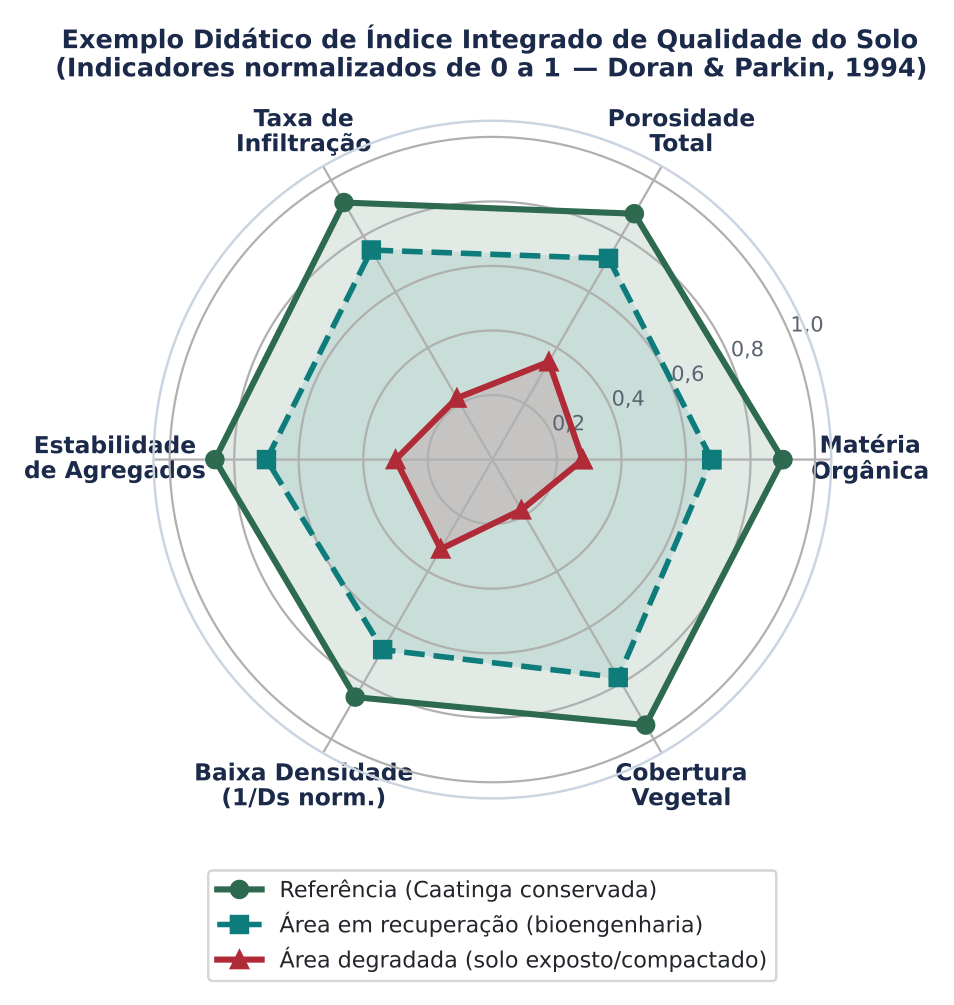
\includegraphics[keepaspectratio]{capitulos/../img/fig09_qualidade_solo_radar.png}}

}

\caption{\label{fig-qualidade_solo_radar}Comparação multivariada de seis
indicadores normalizados de qualidade do solo (\(0\) a \(1\)) entre área
de referência sob Caatinga conservada, área em recuperação com técnicas
de bioengenharia e área degradada com solo exposto e compactado.}

\end{figure}%

Observando os dados plotados na Figura~\ref{fig-qualidade_solo_radar},
nota-se um gradiente nítido de funcionalidade edáfica entre os três
cenários,

\textbf{Referência (Caatinga conservada).} Escores de \(0{,}90\) (MO),
\(0{,}88\) (porosidade total), \(0{,}92\) (taxa de infiltração),
\(0{,}86\) (estabilidade de agregados), \(0{,}85\) (baixa densidade) e
\(0{,}95\) (cobertura vegetal), resultando em
\(\text{IQS} = (0{,}90+0{,}88+0{,}92+0{,}86+0{,}85+0{,}95)/6 = \mathbf{0{,}893}\)
(qualidade muito alta). \textbf{Área em recuperação (bioengenharia).}
Escores entre \(0{,}68\) e \(0{,}78\), com
\(\text{IQS} = (0{,}68+0{,}72+0{,}75+0{,}70+0{,}68+0{,}78)/6 = \mathbf{0{,}718}\)
(qualidade boa em trajetória ascendente, mas com matéria orgânica e
densidade ainda em consolidação). \textbf{Área degradada (solo exposto e
compactado).} Escores colapsados entre \(0{,}18\) (cobertura vegetal) e
\(0{,}35\) (porosidade total), produzindo
\(\text{IQS} = (0{,}28+0{,}35+0{,}22+0{,}30+0{,}32+0{,}18)/6 = \mathbf{0{,}275}\)
(qualidade crítica, exigindo intervenção prioritária na cobertura
superficial e descompactação biológica).

\subsection{Amostragem, referência e normalização do
IQS}\label{amostragem-referuxeancia-e-normalizauxe7uxe3o-do-iqs}

A comparação entre área manejada e referência exige condições
pedológicas e topográficas compatíveis. Profundidade, textura e posição
na vertente influenciam os resultados. Campanhas realizadas em épocas
distintas também podem registrar respostas sazonais, especialmente em
variáveis biológicas e no estado hídrico.

O desenho amostral deve representar a variabilidade espacial. Amostras
de uma faixa compactada por tráfego e de uma área entre linhas podem
pertencer a condições de manejo diferentes. A composição de amostras
pode ser apropriada para certas análises químicas, enquanto propriedades
físicas dependem da preservação de unidades amostrais e de réplicas.

A normalização transforma medidas em pontuações comparáveis segundo uma
função definida. O sentido de melhora precisa acompanhar a função do
indicador. Para pH, o comportamento costuma envolver uma faixa de
adequação, razão pela qual uma regra de crescimento contínuo seria
inadequada. A limitação de pontuações ao intervalo de 0 a 1 também deve
ser explicitada quando utilizada.

O IQS deve ser apresentado junto aos valores individuais e aos pesos.
Duas áreas podem obter a mesma média com limitações distintas, exigindo
medidas diferentes. Protocolos de coleta e determinação devem acompanhar
referências como o
\href{https://www.infoteca.cnptia.embrapa.br/handle/doc/1085209}{Manual
de métodos de análise de solo da Embrapa}, permitindo verificar como
cada valor foi obtido.

\section{Etapa 4 - Exemplos
resolvidos}\label{etapa-4---exemplos-resolvidos-10}

\subsection{Exemplo 11.1 (Básico). Cálculo de Densidade do Solo e
Porosidade Total em Anel
Volumétrico}\label{exemplo-11.1-buxe1sico.-cuxe1lculo-de-densidade-do-solo-e-porosidade-total-em-anel-volumuxe9trico}

\textbf{Situação analisada.} Durante uma campanha prática da disciplina
CHF662, foram coletadas amostras indeformadas (camada
\(0\)-\(10\text{ cm}\)) utilizando anéis de Kopecky de
\(100\text{ cm}^3\) em dois pontos contíguos sobre o mesmo tipo de solo
mineral (\(D_p = 2{,}65\text{ g}\cdot\text{cm}^{-3}\)), um fragmento de
Caatinga conservada e a borda compactada de um acesso de parque eólico.

\textbf{Dados disponíveis.} Volume do anel \(V_t = 100\text{ cm}^3\);
densidade de partículas \(D_p = 2{,}65\text{ g}\cdot\text{cm}^{-3}\).
Massa de solo seco em estufa (\(105\,^\circ\text{C}\)), ponto Caatinga
\(m_{s,1} = 122\text{ g}\); ponto acesso compactado
\(m_{s,2} = 175\text{ g}\).

\textbf{Problema a resolver.} Calcular a densidade do solo (\(D_s\)) e a
porosidade total (\(P_t\)) em ambos os pontos e interpretar o contraste
físico.

\textbf{Fundamento da análise.} Aplicação direta das expressões
\(D_s = m_s / V_t\) e \(P_t = (1 - D_s / D_p)\times 100\%\).

\textbf{Desenvolvimento.} \textbf{Ponto 1, Caatinga conservada,}

\[
D_{s,1} = \frac{122\text{ g}}{100\text{ cm}^3} = 1{,}22\text{ g}\cdot\text{cm}^{-3}
\]

\[
P_{t,1} = \left(1 - \frac{1{,}22}{2{,}65}\right)\times 100\% = (1 - 0{,}4604)\times 100\% = 53{,}96\%
\]

\textbf{Ponto 2, Acesso compactado,}

\[
D_{s,2} = \frac{175\text{ g}}{100\text{ cm}^3} = 1{,}75\text{ g}\cdot\text{cm}^{-3}
\]

\[
P_{t,2} = \left(1 - \frac{1{,}75}{2{,}65}\right)\times 100\% = (1 - 0{,}6604)\times 100\% = 33{,}96\%
\]

\textbf{Diferença de porosidade,}
\(P_{t,2} - P_{t,1} = 33{,}96\% - 53{,}96\% = -20{,}00\) pontos
percentuais (perda relativa de \(37{,}1\%\) do espaço poroso original).

\textbf{Interpretação do resultado.} Caatinga conservada,
\(D_s = 1{,}22\text{ g}\cdot\text{cm}^{-3}\) e \(P_t = 53{,}96\%\).
Acesso compactado, \(D_s = 1{,}75\text{ g}\cdot\text{cm}^{-3}\) e
\(P_t = 33{,}96\%\).

\textbf{Condições de validade.} A compactação aumentou a densidade em
\(0{,}53\text{ g}\cdot\text{cm}^{-3}\) e eliminou exatamente \(20\)
pontos percentuais de porosidade, colapsando prioritariamente os
macroporos de drenagem rápida e explicando o aumento imediato de
escoamento superficial na borda do acesso.

\subsection{Exemplo 11.2 (Básico/Intermediário). Fator de van Bemmelen e
Estoque de Carbono na Camada 0 a 20
cm}\label{11-qualidade-solo-iqs-exemplo-11.2-buxe1sicointermediuxe1rio.-fator-de-van-bemmelen-e-estoque-de-carbono-na-camada-020-cm}

\textbf{Situação analisada.} Um laudo laboratorial reportou carbono
orgânico total de \(18{,}0\text{ g}\cdot\text{kg}^{-1}\) em um solo sob
Caatinga preservada (Área A, com
\(D_s = 1{,}25\text{ g}\cdot\text{cm}^{-3}\)). Em uma pastagem degradada
adjacente no mesmo solo (Área B, com
\(D_s = 1{,}60\text{ g}\cdot\text{cm}^{-3}\)), outro laboratório
expressou o resultado em matéria orgânica total,
\(MO = 12{,}068\text{ g}\cdot\text{kg}^{-1}\).

\textbf{Dados disponíveis.} Camada amostrada,
\(h = 20\text{ cm} = 0{,}20\text{ m}\). Área A,
\(CO_A = 18{,}0\text{ g}\cdot\text{kg}^{-1}\),
\(D_{s,A} = 1{,}25\text{ g}\cdot\text{cm}^{-3}\). Área B,
\(MO_B = 12{,}068\text{ g}\cdot\text{kg}^{-1}\),
\(D_{s,B} = 1{,}60\text{ g}\cdot\text{cm}^{-3}\). Fator de van Bemmelen,
\(1{,}724\).

\textbf{Problema a resolver.} Calcular (a) o teor de \(MO\) na Área A e
o teor de \(CO\) na Área B; (b) o estoque de carbono (\(EC\), em
\(\text{Mg C}\cdot\text{ha}^{-1}\)) na camada \(0\)-\(20\text{ cm}\) das
duas áreas e a perda líquida de carbono.

\textbf{Fundamento da análise.} Conversão via fator de van Bemmelen
(\(MO = 1{,}724 \cdot CO\)) e cálculo da massa total de solo por hectare
na camada de \(0{,}20\text{ m}\) (\(1\text{ ha} = 10.000\text{ m}^2\),
lembrando que
\(1\text{ g}\cdot\text{cm}^{-3} = 1\text{ Mg}\cdot\text{m}^{-3}\)).

\textbf{Desenvolvimento.} \textbf{Etapa 1, Conversão pelo fator de van
Bemmelen,}

\[
MO_A = 18{,}0 \times 1{,}724 = 31{,}032\text{ g}\cdot\text{kg}^{-1} \quad (\text{ou } 3{,}10\%)
\]

\[
CO_B = \frac{12{,}068}{1{,}724} = 7{,}00\text{ g}\cdot\text{kg}^{-1} \quad (\text{ou } 0{,}70\%)
\]

\textbf{Etapa 2, Volume de solo por hectare na camada de
\(0{,}20\text{ m}\),}

\[
V_{\text{ha}} = 10.000\text{ m}^2 \times 0{,}20\text{ m} = 2.000\text{ m}^3\cdot\text{ha}^{-1}
\]

\textbf{Etapa 3, Massa de solo e estoque de carbono (\(EC\)),} Na Área
A, massa de solo
\(= 2.000\text{ m}^3 \times 1{,}25\text{ Mg}\cdot\text{m}^{-3} = 2.500\text{ Mg}\cdot\text{ha}^{-1}\).
Como \(CO_A = 18{,}0\text{ g}\cdot\text{kg}^{-1} = 0{,}018\),

\[
EC_A = 2.500 \times 0{,}018 = 45{,}00\text{ Mg C}\cdot\text{ha}^{-1}
\]

Na Área B, massa de solo
\(= 2.000\text{ m}^3 \times 1{,}60\text{ Mg}\cdot\text{m}^{-3} = 3.200\text{ Mg}\cdot\text{ha}^{-1}\).
Como \(CO_B = 7{,}00\text{ g}\cdot\text{kg}^{-1} = 0{,}007\),

\[
EC_B = 3.200 \times 0{,}007 = 22{,}40\text{ Mg C}\cdot\text{ha}^{-1}
\]

\textbf{Etapa 4, Perda líquida de carbono na camada fixa,}

\[
\Delta EC = 45{,}00 - 22{,}40 = 22{,}60\text{ Mg C}\cdot\text{ha}^{-1} \quad (\text{redução de } 50{,}2\%)
\]

\textbf{Interpretação do resultado.} Área A,
\(MO = 31{,}032\text{ g}\cdot\text{kg}^{-1}\) e
\(EC = 45{,}00\text{ Mg C}\cdot\text{ha}^{-1}\). Área B,
\(CO = 7{,}00\text{ g}\cdot\text{kg}^{-1}\) e
\(EC = 22{,}40\text{ Mg C}\cdot\text{ha}^{-1}\). Perda líquida de
\(22{,}60\text{ Mg C}\cdot\text{ha}^{-1}\).

\textbf{Condições de validade.} Observe um cuidado avançado muito
valorizado em estudos científicos, devido à compactação da Área B
(\(D_s = 1{,}60\) vs.~\(1{,}25\)), uma mesma profundidade fixa de
\(20\text{ cm}\) contém maior massa de solo na área degradada
(\(3.200\text{ Mg}\) vs.~\(2.500\text{ Mg}\)). Em pesquisas de estoques
de carbono de alta precisão, corrige-se essa diferença pelo método da
massa equivalente de solo; ainda assim, a perda aqui já ultrapassa
metade do estoque original.

\subsection{\texorpdfstring{Exemplo 11.3 (Intermediário). Diagnóstico
Químico, Soma de Bases, CTC e Saturação por Bases
(\(V\%\))}{Exemplo 11.3 (Intermediário). Diagnóstico Químico, Soma de Bases, CTC e Saturação por Bases (V\textbackslash\%)}}\label{exemplo-11.3-intermediuxe1rio.-diagnuxf3stico-quuxedmico-soma-de-bases-ctc-e-saturauxe7uxe3o-por-bases-v}

\textbf{Situação analisada.} Compare os laudos químicos de rotina
(camada \(0\)-\(20\text{ cm}\)) de dois solos baianos, Solo 1 (Luvissolo
Crômico sob Caatinga no Semiárido) e Solo 2 (Latossolo Amarelo sob
pastagem degradada nos Tabuleiros Costeiros).

\textbf{Dados disponíveis.} Valores em
\(\text{cmol}_c\cdot\text{dm}^{-3}\),

Solo 1, \(Ca^{2+} = 5{,}40\); \(Mg^{2+} = 2{,}60\); \(K^+ = 0{,}45\);
\(Na^+ = 0{,}15\); \(H^+ + Al^{3+} = 2{,}40\). Solo 2,
\(Ca^{2+} = 1{,}20\); \(Mg^{2+} = 0{,}60\); \(K^+ = 0{,}15\);
\(Na^+ = 0{,}05\); \(H^+ + Al^{3+} = 4{,}00\).

\textbf{Problema a resolver.} Calcular \(SB\), \(CTC\) a pH \(7{,}0\) e
\(V\%\) para os dois solos e classificá-los quanto ao caráter eutrófico
ou distrófico.

\textbf{Fundamento da análise.} Aplicação das equações aditivas de
\(SB\) e \(CTC\) e cálculo da razão percentual
\(V\% = (SB / CTC)\times 100\%\).

\textbf{Desenvolvimento.} \textbf{Solo 1 (Luvissolo, Semiárido),}

\[
SB_1 = 5{,}40 + 2{,}60 + 0{,}45 + 0{,}15 = 8{,}60\text{ cmol}_c\cdot\text{dm}^{-3}
\]

\[
CTC_1 = 8{,}60 + 2{,}40 = 11{,}00\text{ cmol}_c\cdot\text{dm}^{-3}
\]

\[
V\%_1 = \frac{8{,}60}{11{,}00}\times 100\% = 78{,}18\% \quad (\ge 50\% \Rightarrow \textbf{Eutrófico})
\]

\textbf{Solo 2 (Latossolo degradado, Tabuleiro),}

\[
SB_2 = 1{,}20 + 0{,}60 + 0{,}15 + 0{,}05 = 2{,}00\text{ cmol}_c\cdot\text{dm}^{-3}
\]

\[
CTC_2 = 2{,}00 + 4{,}00 = 6{,}00\text{ cmol}_c\cdot\text{dm}^{-3}
\]

\[
V\%_2 = \frac{2{,}00}{6{,}00}\times 100\% = 33{,}33\% \quad (< 50\% \Rightarrow \textbf{Distrófico})
\]

\textbf{Interpretação do resultado.} Solo 1, \(SB = 8{,}60\),
\(CTC = 11{,}00\text{ cmol}_c\cdot\text{dm}^{-3}\) e \(V\% = 78{,}18\%\)
(eutrófico). Solo 2, \(SB = 2{,}00\),
\(CTC = 6{,}00\text{ cmol}_c\cdot\text{dm}^{-3}\) e \(V\% = 33{,}33\%\)
(distrófico).

\textbf{Condições de validade.} O resultado é plenamente coerente com a
pedogênese regional, no Semiárido, a menor lixiviação preserva bases
trocáveis (solos eutróficos, cuja maior limitação costuma ser hídrica e
de profundidade física), enquanto nos ambientes úmidos a intensa
lixiviação combinada à perda de matéria orgânica reduz \(SB\), \(CTC\) e
\(V\%\).

\subsection{Exemplo 11.4 (Avançado). Separação de Macro e
Microporosidade em Mesa de
Tensão}\label{exemplo-11.4-avanuxe7ado.-separauxe7uxe3o-de-macro-e-microporosidade-em-mesa-de-tensuxe3o}

\textbf{Situação analisada.} Uma amostra indeformada de solo
(\(V_t = 100\text{ cm}^3\)) proveniente de uma área em recuperação com
bioengenharia foi saturada por capilaridade, submetida à tensão de
\(6\text{ kPa}\) em mesa de tensão para drenar os macroporos e,
finalmente, seca em estufa a \(105\,^\circ\text{C}\).

\textbf{Dados disponíveis.} Volume total \(V_t = 100\text{ cm}^3\);
densidade da água
\(\rho_{\text{água}} = 1{,}0\text{ g}\cdot\text{cm}^{-3}\). Massas
medidas (já descontada a tara do anel metálico), massa saturada
\(m_{\text{sat}} = 174\text{ g}\); massa após equilíbrio a
\(6\text{ kPa}\), \(m_{6\text{kPa}} = 158\text{ g}\); massa seca em
estufa, \(m_s = 128\text{ g}\).

\textbf{Problema a resolver.} Determinar a porosidade total por
saturação (\(P_t^{\text{sat}}\)), a microporosidade
(\(P_{\text{micro}}\)) e a macroporosidade (\(P_{\text{macro}}\)),
avaliando se há restrição de aeração radicular.

\textbf{Fundamento da análise.} Cálculo dos volumes de água retidos em
cada estado energético (como
\(\rho_{\text{água}} = 1{,}0\text{ g}\cdot\text{cm}^{-3}\), cada
\(1\text{ g}\) de água ocupa \(1\text{ cm}^3\) de poro) divididos pelo
volume total do anel.

\textbf{Desenvolvimento.} \textbf{Etapa 1, Porosidade total por
saturação (água total no anel saturado),}

\[
P_t^{\text{sat}} = \frac{174 - 128}{1{,}0 \times 100}\times 100\% = \frac{46}{100}\times 100\% = 46{,}0\%
\]

\textbf{Etapa 2, Microporosidade (água retida após drenagem a
\(6\text{ kPa}\)),}

\[
P_{\text{micro}} = \frac{158 - 128}{1{,}0 \times 100}\times 100\% = \frac{30}{100}\times 100\% = 30{,}0\%
\]

\textbf{Etapa 3, Macroporosidade (água drenada entre saturação e
\(6\text{ kPa}\)),}

\[
P_{\text{macro}} = \frac{174 - 158}{1{,}0 \times 100}\times 100\% = \frac{16}{100}\times 100\% = 16{,}0\%
\]

\textbf{Conferência aditiva,}
\(P_{\text{micro}} + P_{\text{macro}} = 30{,}0\% + 16{,}0\% = 46{,}0\% = P_t^{\text{sat}}\).

\textbf{Interpretação do resultado.} \(P_t^{\text{sat}} = 46{,}0\%\),
\(P_{\text{micro}} = 30{,}0\%\) e \(P_{\text{macro}} = 16{,}0\%\). Não
há restrição crítica de aeração, pois a macroporosidade supera o limiar
mínimo de \(10\%\).

\textbf{Condições de validade.} A proporção observada (cerca de um terço
de macroporos e dois terços de microporos) aproxima-se do equilíbrio
físico desejável para armazenamento hídrico aliado à drenagem interna e
oxigenação de raízes.

\subsection{Exemplo 11.5 (Avançado). Normalização Linear e Cálculo
Completo do Índice de Qualidade do Solo
(IQS)}\label{exemplo-11.5-avanuxe7ado.-normalizauxe7uxe3o-linear-e-cuxe1lculo-completo-do-uxedndice-de-qualidade-do-solo-iqs}

\textbf{Situação analisada.} Para o Trabalho Prático Final, um grupo
selecionou um Conjunto Mínimo de Dados com quatro indicadores para
avaliar uma encosta submetida à recuperação ambiental, comparando-a a
uma mata de referência no mesmo solo.

\textbf{Dados disponíveis.} Valores medidos na área avaliada e valores
da área de referência,

Matéria Orgânica (\(MO\), ``maior melhor''), avaliada
\(= 16{,}0\text{ g}\cdot\text{kg}^{-1}\); referência
\(= 32{,}0\text{ g}\cdot\text{kg}^{-1}\); peso \(w_1 = 0{,}30\). Taxa de
Infiltração Básica (\(TIB\), ``maior melhor''), avaliada
\(= 24{,}0\text{ mm}\cdot\text{h}^{-1}\); referência
\(= 60{,}0\text{ mm}\cdot\text{h}^{-1}\); peso \(w_2 = 0{,}30\).
Densidade do Solo (\(D_s\), ``menor melhor''), avaliada
\(= 1{,}50\text{ g}\cdot\text{cm}^{-3}\); referência
\(= 1{,}20\text{ g}\cdot\text{cm}^{-3}\); peso \(w_3 = 0{,}20\).
Estabilidade de Agregados (\(DMP\), ``maior melhor''), avaliada
\(= 1{,}25\text{ mm}\); referência \(= 2{,}50\text{ mm}\); peso
\(w_4 = 0{,}20\).

\textbf{Problema a resolver.} Calcular (a) a pontuação normalizada
\(S_i\) de cada indicador; (b) o \(\text{IQS}_{\text{simples}}\) (média
aritmética); e (c) o \(\text{IQS}_{\text{ponderado}}\), indicando qual
atributo representa o gargalo prioritário.

\textbf{Fundamento da análise.} Normalização linear
\(S_i = x_i / x_{\text{ref}}\) para indicadores ``maior melhor'' e
\(S_i = x_{\text{ref}} / x_i\) para indicadores ``menor melhor'',
seguida das médias aritmética e ponderada.

\textbf{Desenvolvimento.} \textbf{Etapa 1, Normalização individual
(escala \(0\) a \(1\)),}

\[
\begin{aligned}
S_{MO} &= \frac{16{,}0}{32{,}0} = 0{,}50 \quad \text{(maior melhor)} \\[3pt]
S_{TIB} &= \frac{24{,}0}{60{,}0} = 0{,}40 \quad \text{(maior melhor)} \\[3pt]
S_{D_s} &= \frac{1{,}20}{1{,}50} = 0{,}80 \quad \text{(menor melhor, razão invertida!)} \\[3pt]
S_{DMP} &= \frac{1{,}25}{2{,}50} = 0{,}50 \quad \text{(maior melhor)}
\end{aligned}
\]

\textbf{Etapa 2, Cálculo do IQS simples,}

\[
\text{IQS}_{\text{simples}} = \frac{0{,}50 + 0{,}40 + 0{,}80 + 0{,}50}{4} = \frac{2{,}20}{4} = 0{,}550
\]

\textbf{Etapa 3, Cálculo do IQS ponderado
(\(\sum w_i = 0{,}30 + 0{,}30 + 0{,}20 + 0{,}20 = 1{,}00\)),}

\[
\text{IQS}_{\text{ponderado}} = (0{,}30 \times 0{,}50) + (0{,}30 \times 0{,}40) + (0{,}20 \times 0{,}80) + (0{,}20 \times 0{,}50)
\]

\[
\text{IQS}_{\text{ponderado}} = 0{,}150 + 0{,}120 + 0{,}160 + 0{,}100 = 0{,}530
\]

\textbf{Interpretação do resultado.} Pontuações, \(S_{MO}=0{,}50\),
\(S_{TIB}=0{,}40\), \(S_{D_s}=0{,}80\), \(S_{DMP}=0{,}50\).
\(\text{IQS}_{\text{simples}} = 0{,}550\) e
\(\text{IQS}_{\text{ponderado}} = 0{,}530\) (qualidade moderada). O
gargalo prioritário é a taxa de infiltração básica
(\(S_{TIB} = 0{,}40\)).

\textbf{Condições de validade.} O \(\text{IQS}_{\text{ponderado}}\)
(\(0{,}530\)) ficou ligeiramente abaixo do simples (\(0{,}550\)) porque
os maiores pesos (\(0{,}30\) cada) recaíram justamente sobre a
infiltração e a matéria orgânica, que apresentaram os piores
desempenhos. Em campo, isso orienta ações focadas em cobertura morta,
descompactação superficial e aporte orgânico.

\section{Etapa 5 - Erros de
interpretação}\label{etapa-5---erros-de-interpretauxe7uxe3o-10}

\subsection{\texorpdfstring{Erro 1, Usar a Fórmula ``Quanto Maior
Melhor'' para Densidade do Solo
(\(D_s\))}{Erro 1, Usar a Fórmula ``Quanto Maior Melhor'' para Densidade do Solo (D\_s)}}\label{erro-1-usar-a-fuxf3rmula-quanto-maior-melhor-para-densidade-do-solo-d_s}

\textbf{Equívoco frequente,} Normalizar \(D_s\) dividindo o valor da
área degradada (\(1{,}75\)) pelo da referência (\(1{,}20\)), obtendo
escore superior a \(1{,}0\) e premiando um solo severamente compactado.

\textbf{Correção técnica,} Para densidade do solo e resistência à
penetração, valores maiores indicam pior qualidade física. Deve-se
aplicar obrigatoriamente a função \textbf{``quanto menor melhor''},
\(S_{D_s} = \min(1;\; D_{s,\text{ref}} / D_{s,\text{avaliado}})\).

\subsection{\texorpdfstring{Erro 2, Confundir Carbono Orgânico (\(CO\))
com Matéria Orgânica
(\(MO\))}{Erro 2, Confundir Carbono Orgânico (CO) com Matéria Orgânica (MO)}}\label{erro-2-confundir-carbono-orguxe2nico-co-com-matuxe9ria-orguxe2nica-mo}

\textbf{Equívoco frequente,} Comparar diretamente um laudo expresso em
\(CO\) (\(\text{g}\cdot\text{kg}^{-1}\)) com outro expresso em \(MO\)
(\(\text{g}\cdot\text{kg}^{-1}\)) sem conversão prévia.

\textbf{Correção técnica,} A matéria orgânica contém carbono, oxigênio,
hidrogênio, nitrogênio e outros elementos; portanto, \(MO\) é sempre
numericamente maior que \(CO\) (\(MO = 1{,}724 \times CO\) pelo fator de
van Bemmelen). Padronize todas as amostras na mesma grandeza antes de
comparar ou calcular estoques de carbono.

\subsection{Erro 3, Comparar Áreas em Solos de Texturas Distintas Sem
Referência
Local}\label{erro-3-comparar-uxe1reas-em-solos-de-texturas-distintas-sem-referuxeancia-local}

\textbf{Equívoco frequente,} Classificar um Neossolo Quartzarênico
arenoso (\(D_s = 1{,}45\text{ g}\cdot\text{cm}^{-3}\)) como degradado
comparando-o a um Latossolo argiloso conservado
(\(D_s = 1{,}05\text{ g}\cdot\text{cm}^{-3}\)).

\textbf{Correção técnica,} Solos arenosos possuem naturalmente maior
densidade e menor \(CTC\) do que solos argilosos bem estruturados. A
área de referência (vegetação nativa) deve sempre pertencer à
\textbf{mesma classe de solo, textura e posição geomorfológica} da área
diagnosticada.

\subsection{\texorpdfstring{Erro 4, Avaliar Resistência à Penetração
(\(RP\)) Sem Registrar a Umidade do
Solo}{Erro 4, Avaliar Resistência à Penetração (RP) Sem Registrar a Umidade do Solo}}\label{erro-4-avaliar-resistuxeancia-uxe0-penetrauxe7uxe3o-rp-sem-registrar-a-umidade-do-solo}

\textbf{Equívoco frequente,} Medir \(RP\) na estação seca no Semiárido,
obter valores acima de \(4{,}0\text{ MPa}\) e diagnosticar compactação
antrópica irreversível.

\textbf{Correção técnica,} A resistência mecânica à penetração aumenta
exponencialmente à medida que o solo seca, devido à coesão entre
partículas e à sucção matricial. Leituras de penetrômetro só são
comparáveis quando realizadas sob umidade controlada (idealmente próxima
à capacidade de campo) ou acompanhadas do teor gravimétrico de umidade.

\section{Etapa 6 - Exercícios de
fixação}\label{etapa-6---exercuxedcios-de-fixauxe7uxe3o-10}

\subsubsection{Nível Básico (Conceitos de Funcionalidade Edáfica e
MDS)}\label{nuxedvel-buxe1sico-conceitos-de-funcionalidade-eduxe1fica-e-mds}

\begin{enumerate}
\def\labelenumi{\arabic{enumi}.}
\item
  Explique por que o conceito contemporâneo de \textbf{Qualidade do
  Solo} (Doran; Parkin, 1994; Karlen et al., 1997) é mais abrangente do
  que a noção tradicional de fertilidade química agrícola.
\item
  Diferencie \textbf{propriedades inerentes} de \textbf{propriedades
  dinâmicas} do solo, citando dois exemplos de cada grupo.
\item
  Qual é o significado físico e matemático do \textbf{fator de van
  Bemmelen (\(1{,}724\))} na conversão entre carbono orgânico total
  (\(CO\)) e matéria orgânica (\(MO\))?
\item
  Por que a \textbf{macroporosidade} é mais sensível à compactação do
  solo do que a porosidade total (\(P_t\)), e qual é o seu limiar
  crítico de aeração radicular?
\item
  Explique por que o \textbf{Carbono da Biomassa Microbiana
  (\(C\text{-BM}\))} e o quociente metabólico (\(q\text{CO}_2\)) são
  indicadores precoces valiosos no monitoramento de áreas degradadas em
  recuperação.
\end{enumerate}

\subsubsection{Nível Intermediário (Cálculos Físicos, Químicos e
IQS)}\label{nuxedvel-intermediuxe1rio-cuxe1lculos-fuxedsicos-quuxedmicos-e-iqs}

\begin{enumerate}
\def\labelenumi{\arabic{enumi}.}
\setcounter{enumi}{5}
\item
  Uma amostra indeformada coletada em anel volumétrico de
  \(100\text{ cm}^3\) apresentou massa de solo seco em estufa de
  \(159\text{ g}\). Considerando densidade de partículas
  \(D_p = 2{,}65\text{ g}\cdot\text{cm}^{-3}\), calcule a densidade do
  solo (\(D_s\)) e a porosidade total (\(P_t\)).
\item
  Um solo sob Caatinga em regeneração apresentou teor de matéria
  orgânica \(MO = 25{,}86\text{ g}\cdot\text{kg}^{-1}\) e densidade do
  solo \(D_s = 1{,}30\text{ g}\cdot\text{cm}^{-3}\) na camada
  \(0\)-\(20\text{ cm}\). Calcule o teor de carbono orgânico total
  (\(CO\), em \(\text{g}\cdot\text{kg}^{-1}\)) usando o fator de van
  Bemmelen e o estoque de carbono (\(EC\), em
  \(\text{Mg C}\cdot\text{ha}^{-1}\)) nessa camada.
\item
  Um laudo químico forneceu os seguintes valores (em
  \(\text{cmol}_c\cdot\text{dm}^{-3}\)), \(Ca^{2+} = 4{,}20\);
  \(Mg^{2+} = 1{,}80\); \(K^+ = 0{,}30\); \(Na^+ = 0{,}10\); e
  \(H^+ + Al^{3+} = 3{,}60\). Calcule \(SB\), \(CTC\) e \(V\%\),
  classificando o solo como eutrófico ou distrófico.
\item
  Em ensaio de mesa de tensão com anel de \(100\text{ cm}^3\)
  (\(\rho_{\text{água}} = 1{,}0\text{ g}\cdot\text{cm}^{-3}\)),
  obtiveram-se as massas (sem a tara do anel),
  \(m_{\text{sat}} = 165\text{ g}\), \(m_{6\text{kPa}} = 157\text{ g}\)
  e \(m_s = 130\text{ g}\). Calcule \(P_t^{\text{sat}}\),
  \(P_{\text{micro}}\) e \(P_{\text{macro}}\), indicando se há risco
  físico à aeração das raízes.
\item
  Calcule o \(\text{IQS}_{\text{simples}}\) de uma parcela degradada a
  partir dos três indicadores abaixo e identifique o indicador de menor
  desempenho,

  \begin{itemize}
  \item
    \(MO\) (maior melhor), parcela \(= 20\text{ g}\cdot\text{kg}^{-1}\);
    referência \(= 40\text{ g}\cdot\text{kg}^{-1}\).
  \item
    \(TIB\) (maior melhor), parcela
    \(= 36\text{ mm}\cdot\text{h}^{-1}\); referência
    \(= 60\text{ mm}\cdot\text{h}^{-1}\).
  \item
    \(D_s\) (menor melhor), parcela
    \(= 1{,}60\text{ g}\cdot\text{cm}^{-3}\); referência
    \(= 1{,}20\text{ g}\cdot\text{cm}^{-3}\).
  \end{itemize}
\end{enumerate}

\subsubsection{Nível Aplicado (Questões Objetivas
A-E)}\label{11-qualidade-solo-iqs-nuxedvel-aplicado-questuxf5es-objetivas-ae}

\begin{enumerate}
\def\labelenumi{\arabic{enumi}.}
\setcounter{enumi}{10}
\item
  A respeito do Conjunto Mínimo de Dados (MDS) para avaliação da
  qualidade do solo (Doran; Parkin, 1994; Vezzani; Mielniczuk, 2009),
  assinale a alternativa correta,

  \begin{enumerate}
  \def\labelenumii{(\Alph{enumii})}
  \item
    Deve conter apenas variáveis químicas de rotina, pois atributos
    físicos e biológicos não se alteram com o manejo da terra.
  \item
    Deve integrar um número enxuto e representativo de indicadores
    físicos, químicos e biológicos sensíveis às mudanças de uso da
    terra.
  \item
    Exige a medição simultânea de todos os 50 atributos laboratoriais
    existentes, independentemente de redundância ou custo.
  \item
    Dispensa a adoção de áreas de referência sob vegetação nativa por
    utilizar valores absolutos idênticos para qualquer textura de solo.
  \item
    Restringe-se ao estudo de solos hidromórficos de várzea.
  \end{enumerate}
\item
  Um solo mineral com densidade de partículas
  \(D_p = 2{,}65\text{ g}\cdot\text{cm}^{-3}\) e densidade do solo
  \(D_s = 1{,}325\text{ g}\cdot\text{cm}^{-3}\) apresenta porosidade
  total (\(P_t\)) exatamente igual a,

  \begin{enumerate}
  \def\labelenumii{(\Alph{enumii})}
  \item
    \(25{,}0\%\).
  \item
    \(40{,}0\%\).
  \item
    \(45{,}0\%\).
  \item
    \(50{,}0\%\).
  \item
    \(60{,}0\%\).
  \end{enumerate}
\item
  Sobre a normalização de indicadores no cálculo do Índice de Qualidade
  do Solo (IQS), é correto afirmar que,

  \begin{enumerate}
  \def\labelenumii{(\Alph{enumii})}
  \item
    Indicadores como taxa de infiltração básica e matéria orgânica
    seguem a função ``quanto menor melhor''.
  \item
    A normalização converte grandezas com unidades diferentes para uma
    escala adimensional comum (como \(0\) a \(1\)), possibilitando a
    agregação matemática.
  \item
    A densidade do solo deve ser normalizada pela razão
    \(D_{s,\text{avaliado}} / D_{s,\text{referência}}\) para que solos
    mais compactados recebam notas maiores.
  \item
    O uso de pesos diferenciados (\(w_i\)) é proibido em índices de
    qualidade ambiental.
  \item
    Um IQS igual a \(0{,}25\) indica funcionalidade edáfica superior à
    da área de referência.
  \end{enumerate}
\item
  Se uma amostra de solo apresenta teor de carbono orgânico total
  \(CO = 10{,}0\text{ g}\cdot\text{kg}^{-1}\), o teor estimado de
  matéria orgânica (\(MO\)) pelo fator de van Bemmelen (\(1{,}724\)) é,

  \begin{enumerate}
  \def\labelenumii{(\Alph{enumii})}
  \item
    \(5{,}80\text{ g}\cdot\text{kg}^{-1}\).
  \item
    \(10{,}00\text{ g}\cdot\text{kg}^{-1}\).
  \item
    \(15{,}80\text{ g}\cdot\text{kg}^{-1}\).
  \item
    \(17{,}24\text{ g}\cdot\text{kg}^{-1}\).
  \item
    \(27{,}24\text{ g}\cdot\text{kg}^{-1}\).
  \end{enumerate}
\item
  Na interpretação do gráfico radar de qualidade do solo
  (Figura~\ref{fig-qualidade_solo_radar}), uma área degradada que
  apresenta valores normalizados muito baixos em \emph{cobertura
  vegetal} (\(0{,}18\)) e \emph{taxa de infiltração} (\(0{,}22\))
  sinaliza prioritariamente,

  \begin{enumerate}
  \def\labelenumii{(\Alph{enumii})}
  \item
    Alta resiliência física da superfície do solo frente a chuvas
    intensas.
  \item
    Predomínio de drenagem profunda com risco nulo de escoamento
    superficial.
  \item
    Forte vulnerabilidade ao impacto da gota de chuva, selamento
    superficial e geração de enxurrada erosiva.
  \item
    Excesso de matéria orgânica humificada na camada superficial.
  \item
    Equivalência funcional plena em relação à Caatinga conservada.
  \end{enumerate}
\end{enumerate}

\section{Etapa 7 - Questões de
aplicação}\label{etapa-7---questuxf5es-de-aplicauxe7uxe3o-10}

\subsection{Atenção às Armadilhas em Questões de
Solos}\label{atenuxe7uxe3o-uxe0s-armadilhas-em-questuxf5es-de-solos}

Em provas de Geografia e concursos ambientais, dois detalhes costumam
decidir questões, (1) verificar se a tabela fornece \textbf{Carbono
Orgânico (\(CO\))} ou \textbf{Matéria Orgânica (\(MO\))} antes de
multiplicar ou dividir por \(1{,}724\); e (2) observar o sentido da
normalização (``maior melhor'' vs.~``menor melhor'') em indicadores como
\(D_s\) e \(RP\).

\begin{enumerate}
\def\labelenumi{\arabic{enumi}.}
\setcounter{enumi}{15}
\item
  \textbf{{[}Questão Autoral, Estilo ENADE / Geografia{]}} Dois talhões
  localizados sobre a mesma classe de solo no Semiárido Baiano foram
  avaliados quanto à funcionalidade edáfica. O Talhão X (Caatinga
  conservada) exibiu \(D_s = 1{,}20\text{ g}\cdot\text{cm}^{-3}\),
  \(P_{\text{macro}} = 18\%\), \(MO = 30\text{ g}\cdot\text{kg}^{-1}\) e
  \(TIB = 65\text{ mm}\cdot\text{h}^{-1}\). O Talhão Y (área de
  empréstimo de terra após obra viária) apresentou
  \(D_s = 1{,}72\text{ g}\cdot\text{cm}^{-3}\),
  \(P_{\text{macro}} = 6\%\), \(MO = 7\text{ g}\cdot\text{kg}^{-1}\) e
  \(TIB = 9\text{ mm}\cdot\text{h}^{-1}\). Com base nesses resultados,
  analise as asserções,

  \begin{quote}
  \textbf{I.} O Talhão Y encontra-se fisicamente degradado e sob elevada
  suscetibilidade ao escoamento superficial concentrado e à erosão
  hídrica.\\
  \textbf{PORQUE}\\
  \textbf{II.} A perda de matéria orgânica e o colapso da
  macroporosidade abaixo de \(10\%\) comprometem a estabilidade dos
  agregados e reduzem drasticamente a taxa de infiltração básica do
  solo.
  \end{quote}

  A respeito dessas asserções, assinale a opção correta,

  \begin{enumerate}
  \def\labelenumii{(\Alph{enumii})}
  \item
    As asserções I e II são proposições verdadeiras, e a II é uma
    justificativa correta da I.
  \item
    As asserções I e II são proposições verdadeiras, mas a II não é uma
    justificativa correta da I.
  \item
    A asserção I é uma proposição verdadeira, e a II é uma proposição
    falsa.
  \item
    A asserção I é uma proposição falsa, e a II é uma proposição
    verdadeira.
  \item
    As asserções I e II são proposições falsas.
  \end{enumerate}
\item
  \textbf{{[}Questão Autoral, Estilo Concurso Analista Ambiental{]}} Em
  um diagnóstico pedológico para elaboração de PRAD, a análise química
  da camada superficial de uma área degradada revelou Soma de Bases
  \(SB = 3{,}20\text{ cmol}_c\cdot\text{dm}^{-3}\) e Capacidade de Troca
  Catiônica a pH \(7{,}0\) de
  \(CTC = 8{,}00\text{ cmol}_c\cdot\text{dm}^{-3}\). Com base nesses
  valores, a saturação por bases (\(V\%\)) e a classificação química do
  solo são, respectivamente,

  \begin{enumerate}
  \def\labelenumii{(\Alph{enumii})}
  \item
    \(25{,}0\%\), eutrófico.
  \item
    \(40{,}0\%\), distrófico.
  \item
    \(40{,}0\%\), eutrófico.
  \item
    \(60{,}0\%\), distrófico.
  \item
    \(60{,}0\%\), eutrófico.
  \end{enumerate}
\item
  \textbf{{[}Questão Autoral, Estilo Concurso Perito / Geógrafo
  Ambiental{]}} Sobre a escolha e o uso de indicadores biológicos na
  avaliação da qualidade do solo (Vezzani; Mielniczuk, 2009; Karlen et
  al., 1997), assinale a alternativa \textbf{INCORRETA},

  \begin{enumerate}
  \def\labelenumii{(\Alph{enumii})}
  \item
    A fauna edáfica (como minhocas, formigas e térmitas) contribui para
    a formação de bioporos que aumentam a infiltração de água e a
    aeração do perfil.
  \item
    O carbono da biomassa microbiana tende a responder mais rapidamente
    a mudanças de uso da terra do que o estoque total de carbono
    orgânico.
  \item
    Valores muito elevados de quociente metabólico (\(q\text{CO}_2\)) em
    áreas degradadas podem indicar estresse sobre a comunidade
    microbiana, que despende maior proporção de carbono em respiração de
    manutenção.
  \item
    A cobertura vegetal e a serapilheira modulam a temperatura e a
    umidade do solo, favorecendo a atividade biológica em ambientes
    tropicais e semiáridos.
  \item
    Indicadores biológicos dispensam totalmente a avaliação de densidade
    do solo e infiltração, pois a presença de micro-organismos elimina a
    compactação mecânica em poucos dias.
  \end{enumerate}
\end{enumerate}

\section{Etapa 8 - Gabarito
comentado}\label{etapa-8---gabarito-comentado-10}

\subsection{Resoluções Completas, Exercícios de Fixação (1 a
15)}\label{resoluuxe7uxf5es-completas-exercuxedcios-de-fixauxe7uxe3o-1-a-15-1}

\begin{enumerate}
\def\labelenumi{\arabic{enumi}.}
\item
  A fertilidade química clássica foca na disponibilidade imediata de
  nutrientes para produção vegetal. Já a \textbf{Qualidade do Solo}
  avalia o conjunto das funções ecossistêmicas (regulação hídrica,
  filtragem de poluentes, estocagem de carbono, sustentação da
  biodiversidade e resistência à erosão), exigindo integração de
  atributos físicos, químicos e biológicos.
\item
  \textbf{Propriedades inerentes.} Dependem dos fatores de formação e
  variam pouco em escala humana (por exemplo, textura do solo e
  mineralogia da fração argila). \textbf{Propriedades dinâmicas.}
  Respondem em curto e médio prazo ao manejo e à degradação (por
  exemplo, densidade do solo, matéria orgânica, estabilidade de
  agregados e taxa de infiltração básica).
\item
  O fator \(1{,}724\) deriva da premissa clássica de que a matéria
  orgânica do solo contém aproximadamente \(58\%\) de carbono em sua
  composição mássica (\(1 / 0{,}58 = 1{,}7241\dots\)). Assim,
  \(MO = 1{,}724 \times CO\) e \(CO = MO / 1{,}724\).
\item
  Sob pressão mecânica (máquinas, pisoteio), os poros maiores
  (macroporos, \(>50\,\mu\text{m}\)) são os primeiros a colapsar, muitas
  vezes transformando-se em microporos; logo, \(P_{\text{macro}}\) cai
  muito mais intensamente do que \(P_t\). O limiar crítico clássico para
  aeração adequada das raízes é de \(\mathbf{10\%}\) do volume do solo.
\item
  O \(C\text{-BM}\) representa a fração viva e ativa do carbono do solo,
  reagindo em poucos meses ao manejo antes que alterações sejam
  mensuráveis no \(CO\) total. O \(q\text{CO}_2\)
  (\(RBS / C\text{-BM}\)) complementa essa leitura ao revelar se a biota
  está em equilíbrio eficiente ou sob estresse energético.
\item
  \textbf{Passo a passo,}
  \(D_s = 159\text{ g} / 100\text{ cm}^3 = \mathbf{1{,}59\text{ g}\cdot\text{cm}^{-3}}\).
  \(P_t = (1 - 1{,}59 / 2{,}65)\times 100\% = (1 - 0{,}60)\times 100\% = \mathbf{40{,}0\%}\).
\item
  \textbf{Passo a passo,}
  \(CO = 25{,}86 / 1{,}724 = \mathbf{15{,}00\text{ g}\cdot\text{kg}^{-1}}\)
  (ou \(0{,}015\text{ kg C}\cdot\text{kg}^{-1}\) solo). Volume de solo
  na camada \(0\)-\(20\text{ cm}\) em \(1\text{ ha}\),
  \(10.000\text{ m}^2 \times 0{,}20\text{ m} = 2.000\text{ m}^3\). Massa
  de solo,
  \(2.000\text{ m}^3 \times 1{,}30\text{ Mg}\cdot\text{m}^{-3} = 2.600\text{ Mg}\cdot\text{ha}^{-1}\).
  Estoque de carbono,
  \(EC = 2.600 \times 0{,}015 = \mathbf{39{,}00\text{ Mg C}\cdot\text{ha}^{-1}}\).
\item
  \textbf{Passo a passo,}
  \(SB = 4{,}20 + 1{,}80 + 0{,}30 + 0{,}10 = \mathbf{6{,}40\text{ cmol}_c\cdot\text{dm}^{-3}}\).
  \(CTC = 6{,}40 + 3{,}60 = \mathbf{10{,}00\text{ cmol}_c\cdot\text{dm}^{-3}}\).
  \(V\% = (6{,}40 / 10{,}00)\times 100\% = \mathbf{64{,}0\%}\). Como
  \(V\% \ge 50\%\), o solo é classificado como \textbf{eutrófico}.
\item
  \textbf{Passo a passo,}
  \(P_t^{\text{sat}} = (165 - 130)/100 \times 100\% = \mathbf{35{,}0\%}\).
  \(P_{\text{micro}} = (157 - 130)/100 \times 100\% = \mathbf{27{,}0\%}\).
  \(P_{\text{macro}} = (165 - 157)/100 \times 100\% = \mathbf{8{,}0\%}\).
  Como \(P_{\text{macro}} = 8{,}0\% < 10\%\), há \textbf{risco físico de
  restrição à aeração radicular} e à drenagem rápida.
\item
  \textbf{Passo a passo,} \(S_{MO} = 20 / 40 = 0{,}50\) (maior melhor);
  \(S_{TIB} = 36 / 60 = 0{,}60\) (maior melhor);
  \(S_{D_s} = 1{,}20 / 1{,}60 = 0{,}75\) (menor melhor).
  \(\text{IQS}_{\text{simples}} = (0{,}50 + 0{,}60 + 0{,}75) / 3 = 1{,}85 / 3 \approx \mathbf{0{,}617}\).
  O indicador de menor desempenho é a \textbf{matéria orgânica
  (\(S_{MO} = 0{,}50\))}.
\item
  \textbf{Gabarito, (B).} O MDS seleciona um conjunto enxuto, sensível e
  multidisciplinar (físico, químico e biológico), sempre calibrado em
  relação a um solo de referência local.
\item
  \textbf{Gabarito, (D).}
  \(P_t = (1 - 1{,}325 / 2{,}65)\times 100\% = (1 - 0{,}50)\times 100\% = \mathbf{50{,}0\%}\).
\item
  \textbf{Gabarito, (B).} A normalização coloca indicadores heterogêneos
  na mesma escala adimensional (\(0\) a \(1\)). (A) inverte o sentido de
  \(TIB\) e \(MO\); (C) inverte o sentido de \(D_s\); (D) é falsa pois
  índices ponderados são amplamente usados; (E) é falsa pois \(0{,}25\)
  representa qualidade muito baixa.
\item
  \textbf{Gabarito, (D).}
  \(MO = 10{,}0 \times 1{,}724 = \mathbf{17{,}24\text{ g}\cdot\text{kg}^{-1}}\).
\item
  \textbf{Gabarito, (C).} Cobertura vegetal mínima (\(0{,}18\)) expõe o
  solo ao impacto direto das gotas, agravando o selamento e derrubando a
  infiltração (\(0{,}22\)), o que amplifica o escoamento superficial
  erosivo.
\end{enumerate}

\subsection{Resoluções Completas, Questões ENADE e Concursos (16 a
18)}\label{resoluuxe7uxf5es-completas-questuxf5es-enade-e-concursos-16-a-18-1}

\begin{enumerate}
\def\labelenumi{\arabic{enumi}.}
\setcounter{enumi}{15}
\item
  \textbf{Gabarito, (A).} Ambas as asserções são verdadeiras e mantêm
  nexo causal rigoroso, a elevação da densidade
  (\(1{,}72\text{ g}\cdot\text{cm}^{-3}\)), o colapso da macroporosidade
  (\(6\% < 10\%\)) e a queda acentuada da matéria orgânica reduzem
  drasticamente a infiltração (\(9\text{ mm}\cdot\text{h}^{-1}\)),
  tornando o Talhão Y altamente suscetível ao escoamento superficial
  erosivo.
\item
  \textbf{Gabarito, (B).}
  \(V\% = (3{,}20 / 8{,}00)\times 100\% = \mathbf{40{,}0\%}\). Como
  \(V\% < 50\%\), o solo é \textbf{distrófico}.
\item
  \textbf{Gabarito, (E).} A alternativa (E) é incorreta porque a
  recuperação biológica da estrutura física do solo compactado ocorre
  gradualmente (meses a anos) e requer diagnóstico conjunto com
  indicadores físicos (\(D_s\), \(P_{\text{macro}}\), \(TIB\) e \(RP\)).
\end{enumerate}

\section{Etapa 9 - Síntese
conceitual}\label{etapa-9---suxedntese-conceitual-10}

\textbf{Funcionalidade edáfica.} A qualidade do solo mede sua capacidade
de infiltrar água, ciclar nutrientes, estocar carbono e sustentar vida,
avaliada sempre contra um solo de referência da mesma classe pedológica.
\textbf{Tríade do MDS.} Indicadores \textbf{físicos} (\(D_s\), \(P_t\),
\(P_{\text{macro}}\), \(DMP\), \(TIB\), \(RP\)), \textbf{químicos}
(\(CO\), \(MO = 1{,}724 \cdot CO\), pH, \(SB\), \(CTC\), \(V\%\)) e
\textbf{biológicos} (\(C\text{-BM}\), \(RBS\), \(q\text{CO}_2\), fauna e
cobertura vegetal). \textbf{Cálculo do IQS.} Padronize cada atributo
entre \(0\) e \(1\) respeitando a direção (``maior melhor''
\(= x_i/x_{\text{ref}}\); ``menor melhor'' \(= x_{\text{ref}}/x_i\)) e
agregue via média simples ou ponderada, mantendo o gráfico radar para
evidenciar gargalos individuais.

\section{Etapa 10 - Verificação da
aprendizagem}\label{etapa-10---verificauxe7uxe3o-da-aprendizagem-10}

Marque \textbf{V} (Verdadeiro) ou \textbf{F} (Falso) e confira o
gabarito,

\begin{enumerate}
\def\labelenumi{\arabic{enumi}.}
\item
  ( ) Quanto maior a densidade do solo (\(D_s\)) para uma mesma
  densidade de partículas (\(D_p\)), menor será a porosidade total
  (\(P_t\)).
\item
  ( ) Pelo fator de van Bemmelen (\(1{,}724\)), um solo com
  \(17{,}24\text{ g}\cdot\text{kg}^{-1}\) de matéria orgânica possui
  aproximadamente \(10{,}0\text{ g}\cdot\text{kg}^{-1}\) de carbono
  orgânico total.
\item
  ( ) Um solo com saturação por bases \(V\% = 72\%\) é classificado como
  distrófico devido à predominância de alumínio trocável.
\item
  ( ) No cálculo do IQS, a densidade do solo (\(D_s\)) segue a função
  ``quanto menor melhor'', enquanto a taxa de infiltração básica
  (\(TIB\)) segue ``quanto maior melhor''.
\end{enumerate}

\textbf{Gabarito do verificação da aprendizagem,} 1-\textbf{V}
\textbar-\textbf{V} \textbar-\textbf{F}~(\(V\% \ge 50\%\) caracteriza
solo eutrófico) \textbar-\textbf{V}.

\chapter{Diagnóstico de Processos de Degradação Ambiental e Erosão
Linear}\label{cap:degradacao_erosao_linear}

A degradação por erosão resulta da interação entre disponibilidade de
material, energia do escoamento e caminhos de transporte. Reconhecer a
forma erosiva ajuda a selecionar o método de avaliação, enquanto a
interpretação do mecanismo exige observar drenagem, materiais e evolução
temporal.

\section{Etapa 1 - Objetivos de
aprendizagem}\label{etapa-1---objetivos-de-aprendizagem-11}

A aprendizagem envolve diferenciar processos erosivos, aplicar
estimativas de perda de solo e interpretar medições repetidas. O
estudante deve reconhecer a escala de validade de cada método e explicar
como os resultados se relacionam ao transporte e à deposição de
sedimentos.

\section{Etapa 2 - Conhecimentos
necessários}\label{etapa-2---conhecimentos-necessuxe1rios-11}

A leitura retoma balanço de massa, densidade do solo, área e volume.
Taxa de perda em toneladas por hectare e por ano, volume erodido em uma
feição e carga sólida transportada no canal representam grandezas
distintas e exigem procedimentos próprios.

\section{Etapa 3 - Fundamentação
teórica}\label{etapa-3---fundamentauxe7uxe3o-teuxf3rica-11}

\subsection{Vocabulário Técnico e Símbolos do Capítulo
12}\label{vocabuluxe1rio-tuxe9cnico-e-suxedmbolos-do-capuxedtulo-12}

\textbf{\emph{Splash} (salpicamento),} desagregação de partículas do
solo pelo impacto cinético direto das gotas de chuva, gerando crosta de
selamento superficial. \textbf{\emph{Piping} (erosão em túneis ou
tubular),} remoção interna de partículas finas do solo por fluxos
subsuperficiais concentrados, criando dutos que colapsam e aceleram o
avanço de voçorocas. \textbf{USLE
(\(A = R \cdot K \cdot L \cdot S \cdot C \cdot P\)).} Modelo empírico
que estima a perda média anual de solo por erosão laminar e em sulcos
(\(\text{t}\cdot\text{ha}^{-1}\cdot\text{ano}^{-1}\)).

\(T\), limite de tolerância de perda de solo
(\(\text{t}\cdot\text{ha}^{-1}\cdot\text{ano}^{-1}\)), correspondente à
taxa máxima de erosão compatível com a renovação pedogenética e
manutenção da funcionalidade do perfil. \(h\), taxa de rebaixamento da
superfície do solo (\(\text{mm}\cdot\text{ano}^{-1}\)), vinculada à
perda de massa pela densidade do solo (\(D_s\)). \(\Delta \bar{h}\),
variação média de exposição em uma malha de pinos de erosão
(\(\text{mm}\)); valores positivos indicam erosão (rebaixamento) e
negativos indicam deposição (soterramento).

\(SDR\), Razão de Aporte de Sedimentos (\emph{Sediment Delivery Ratio},
adimensional entre \(0\) e \(1\)), fração do solo erodido nas vertentes
que efetivamente alcança o exutório ou reservatório da bacia.

\subsection{Mecânica e Sequência Evolutiva da Erosão
Hídrica}\label{mecuxe2nica-e-sequuxeancia-evolutiva-da-erosuxe3o-huxeddrica}

A erosão hídrica acelerada resulta do desequilíbrio entre a
\textbf{erosividade} (capacidade da chuva e do escoamento de desprender
e transportar partículas) e a \textbf{resistência do sistema
solo-vegetação} (cobertura, agregação, rugosidade e infiltração).
Conforme sintetizam Guerra e Cunha (1996), Ross (1994) e Cavalcanti
(2006), o processo evolui em estágios progressivos de severidade física
e de custo exponencial de recuperação
(Figura~\ref{fig-evolucao_erosao_linear}).

\begin{figure}[H]

\centering{

\pandocbounded{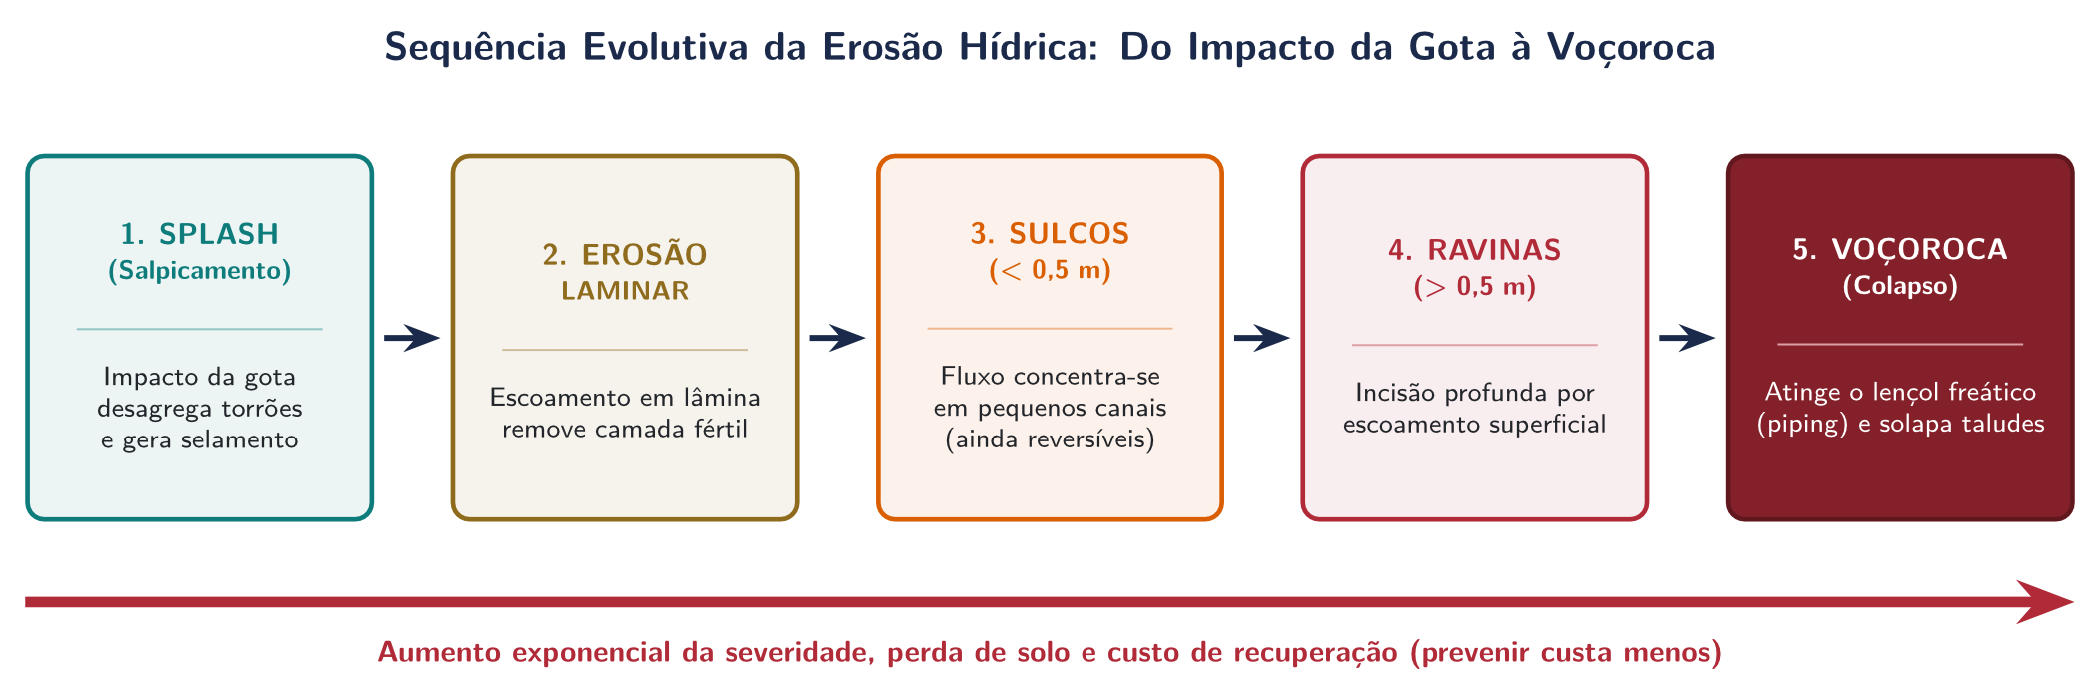
\includegraphics[keepaspectratio]{capitulos/../img/fig10_evolucao_erosao_linear.png}}

}

\caption{\label{fig-evolucao_erosao_linear}Sequência evolutiva dos
processos erosivos hídricos, do impacto da gota (\emph{splash}) ao
colapso por voçorocamento, evidenciando o aumento exponencial da
severidade e do custo de recuperação.}

\end{figure}%

Cada estágio possui diagnóstico morfológico e mecânico próprio,

\textbf{Impacto da gota (\emph{splash}) e selamento superficial,} quando
o solo perde cobertura vegetal e serapilheira, as gotas de chuva atingem
diretamente os agregados superficiais, rompendo-os e lançando partículas
finas (argila e silte) em suspensão. Essas partículas obstruem os poros
superficiais, formando uma crosta delgada (\textbf{selamento
superficial}) que reduz drasticamente a taxa de infiltração básica.
\textbf{Erosão laminar (entressulcos).} Com a infiltração bloqueada pelo
selamento ou pela compactação, a água acumula-se e escoa em lâmina
difusa sobre a vertente, removendo silenciosamente a camada mais fértil
do horizonte A (matéria orgânica, sementes e nutrientes). Por não abrir
grandes cicatrizes visíveis no início, costuma passar despercebida até
que aflorem raízes, cascalhos ou horizontes subsuperficiais mais claros.

\textbf{Sulcos erosivos (\(< 0{,}5\text{ m}\) de profundidade).}
Irregularidades microtopográficas, marcas de pneus ou linhas de plantio
morro abaixo concentram a lâmina d'água em filetes de maior velocidade e
tensão cisalhante. Os canais rasos assim abertos são denominados sulcos
e, em geral, ainda podem ser corrigidos por práticas conservacionistas e
manejo superficial do solo. \textbf{Ravinas (\(> 0{,}5\text{ m}\) de
profundidade, sem atingir o lençol freático).} Se o escoamento
superficial concentrado não for dissipado, os sulcos aprofundam-se e
alargam-se, tornando-se incisões permanentes que não são eliminadas por
preparo comum do solo. O agente dominante na ravina ainda é o
\textbf{escoamento superficial concentrado}, que excava o leito e
expande o canal remontantemente (de jusante para montante).

\textbf{Voçorocas (estágio de colapso integrado).} Representam a forma
mais avançada e destrutiva da erosão linear. Diferenciam-se das ravinas
não apenas pelas dimensões métricas, mas sobretudo pelo \textbf{processo
hidrogeomorfológico}, a incisão atinge o \textbf{lençol freático} (ou
zonas de fluxo subsuperficial saturado). Passam então a atuar
simultaneamente o escoamento superficial, a erosão subsuperficial em
túneis (\textbf{\emph{piping}}) e a exfiltração na base das paredes,
provocando \textbf{solapamento} e escorregamentos sucessivos dos taludes
laterais e da cabeceira, mesmo em períodos sem chuva intensa.

\subsection{Instabilidade de Margens Fluviais, Degradação Ripária e
Assoreamento}\label{instabilidade-de-margens-fluviais-degradauxe7uxe3o-ripuxe1ria-e-assoreamento}

Na escala da bacia hidrográfica, a erosão das vertentes articula-se
diretamente à dinâmica dos canais fluviais e das Áreas de Preservação
Permanente (APPs) marginais,

\textbf{Degradação ripária e colapso de margens.} A supressão da mata
ciliar elimina a malha radicular que confere coesão mecânica aos
barrancos (tema aprofundado na bioengenharia do Capítulo 13) e expõe a
margem ao impacto direto da corrente fluvial. A erosão na base do talude
marginal (\emph{undercutting}) gera quedas em bloco e alargamento
desordenado da calha. \textbf{Assoreamento de canais, açudes e
reservatórios.} Quando o aporte de sedimentos oriundo das vertentes e
margens excede a capacidade de transporte do curso d'água, ocorre
deposição no leito. No Semiárido Baiano, o assoreamento reduz
rapidamente o volume útil de açudes, barreiros e pequenos barramentos
comunitários, agrava a vulnerabilidade hídrica nas estiagens e eleva a
turbidez da água.

\subsection{Equação Universal de Perda de Solo
(USLE)}\label{equauxe7uxe3o-universal-de-perda-de-solo-usle}

Desenvolvida por Wischmeier e Smith (1978) a partir de milhares de
parcelas experimentais e amplamente calibrada para condições tropicais e
brasileiras, a \textbf{Equação Universal de Perda de Solo (USLE)} estima
a perda média anual de solo por erosão laminar e em sulcos a partir do
produto de seis fatores físicos e de manejo.

\subsection{Equação Universal de Perda de Solo (USLE) e Conversão para
Rebaixamento}\label{equauxe7uxe3o-universal-de-perda-de-solo-usle-e-conversuxe3o-para-rebaixamento}

\[
A = R \cdot K \cdot L \cdot S \cdot C \cdot P
\]

\(A\), perda média anual estimada de solo
(\(\text{t}\cdot\text{ha}^{-1}\cdot\text{ano}^{-1}\)). \(R\), fator de
\textbf{erosividade da chuva}
(\(\text{MJ}\cdot\text{mm}\cdot\text{ha}^{-1}\cdot\text{h}^{-1}\cdot\text{ano}^{-1}\));
expressa a energia cinética e intensidade máxima das precipitações ao
longo do ano. \(K\), fator de \textbf{erodibilidade do solo}
(\(\text{t}\cdot\text{ha}\cdot\text{h}\cdot\text{ha}^{-1}\cdot\text{MJ}^{-1}\cdot\text{mm}^{-1}\));
reflete a suscetibilidade intrínseca do solo à erosão (textura, matéria
orgânica, estrutura e permeabilidade). \(L\) e \(S\), fatores
topográficos de \textbf{comprimento de rampa (\(L\))} e
\textbf{declividade (\(S\))} (adimensionais, frequentemente agrupados
como fator \(LS\)). Quanto maior e mais íngreme a vertente, maior o
valor de \(LS\).

\(C\), fator de \textbf{uso, manejo e cobertura vegetal} (adimensional,
entre \(\approx 0{,}001\) em floresta densa e \(1{,}00\) em solo
continuamente descoberto e mobilizado). \(P\), fator de \textbf{práticas
conservacionistas} (adimensional, de \(1{,}00\) em plantio morro abaixo
até \(\approx 0{,}50\) em plantio em contorno ou \(0{,}20\)-\(0{,}40\)
com terraceamento e cordões vegetados).

\textbf{Relação entre Perda de Massa (\(A\)) e Rebaixamento Superficial
(\(h\)),} Como \(1\text{ ha} = 10.000\text{ m}^2\), uma lâmina de
\(1\text{ mm}\) (\(0{,}001\text{ m}\)) de solo em \(1\text{ ha}\) possui
volume de \(10\text{ m}^3\). Multiplicando pela densidade do solo
(\(D_s\) em
\(\text{t}\cdot\text{m}^{-3} = \text{g}\cdot\text{cm}^{-3}\)), cada
\(1\text{ mm}\) corresponde a \(10 \cdot D_s\) toneladas por hectare,

\[
h\,(\text{mm}\cdot\text{ano}^{-1}) = \frac{A\,(\text{t}\cdot\text{ha}^{-1}\cdot\text{ano}^{-1})}{10 \cdot D_s} \qquad \Longleftrightarrow \qquad A = 10 \cdot D_s \cdot h
\]

É fundamental destacar duas características essenciais da USLE, (1) o
produto \(R \cdot K \cdot L \cdot S\) representa o \textbf{potencial
natural de erosão} (o solo completamente descoberto e sem práticas
conservacionistas); e (2) os fatores \(C\) e \(P\) são os elementos
sobre os quais a gestão territorial e o manejo atuam diretamente,
podendo reduzir as perdas em mais de \(95\%\), conforme ilustrado na
Figura~\ref{fig-usle_sensibilidade}. Além disso, a USLE \textbf{não
modela erosão em ravinas profundas, voçorocas ou margens fluviais}, nem
quantifica diretamente a deposição na base da vertente. Para estimar o
sedimento que chega a um reservatório, associa-se a USLE à Razão de
Aporte de Sedimentos (\(SDR\)).

\begin{figure}[H]

\centering{

\pandocbounded{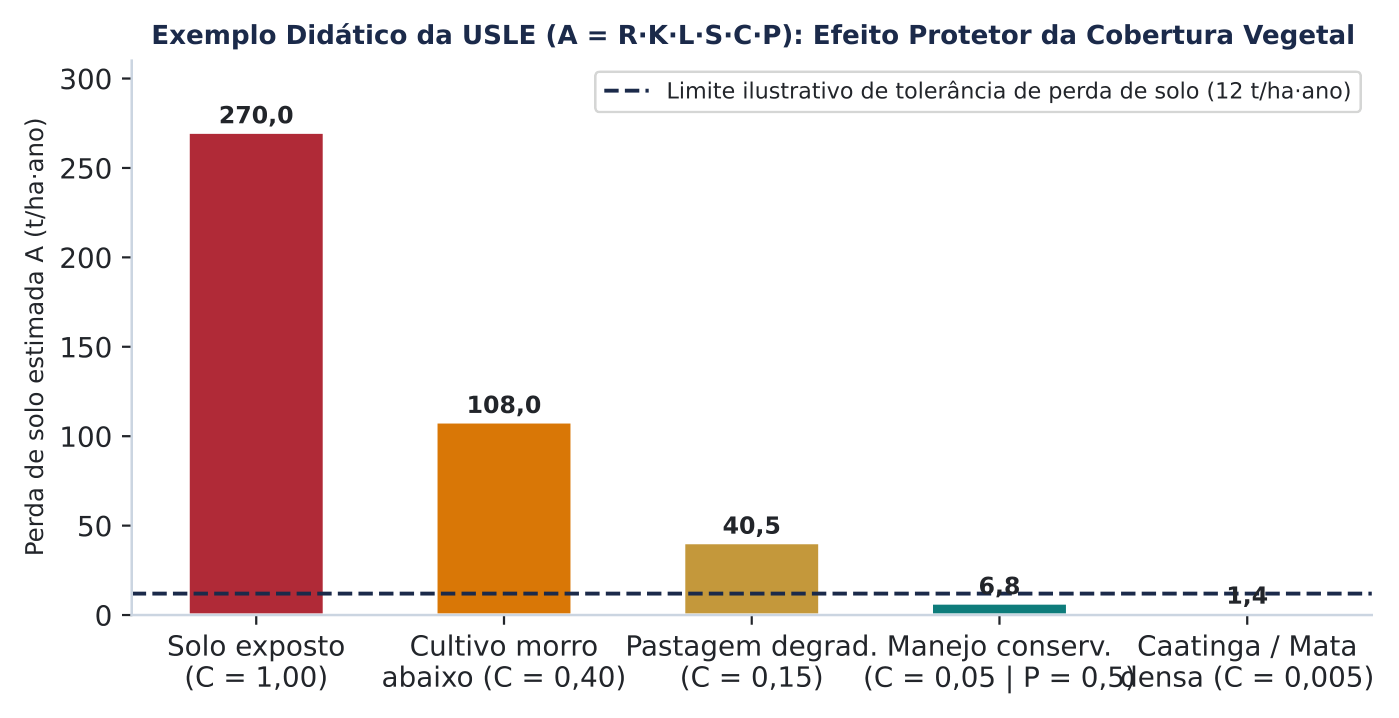
\includegraphics[keepaspectratio]{capitulos/../img/fig11_usle_sensibilidade.png}}

}

\caption{\label{fig-usle_sensibilidade}Análise de sensibilidade da
Equação Universal de Perda de Solo (\(R = 6.000\), \(K = 0{,}03\),
\(LS = 1{,}5\), potencial natural de
\(270\text{ t}\cdot\text{ha}^{-1}\cdot\text{ano}^{-1}\)) sob cinco
cenários de cobertura e manejo frente ao limite ilustrativo de
tolerância (\(12\text{ t}\cdot\text{ha}^{-1}\cdot\text{ano}^{-1}\)).}

\end{figure}%

\subsection{Protocolos Quantitativos de Diagnóstico e Monitoramento em
Campo}\label{protocolos-quantitativos-de-diagnuxf3stico-e-monitoramento-em-campo}

Modelos como a USLE fornecem estimativas de planejamento, mas o
diagnóstico rigoroso de processos ativos em campo requer medições
diretas e rastreáveis,

\textbf{Método dos Pinos de Erosão.} Consiste na cravação vertical de
vergalhões metálicos ou pinos rígidos (tipicamente de \(30\) a
\(50\text{ cm}\) de comprimento) dispostos em malha ou transectos ao
longo da vertente ou talude, deixando uma altura inicial exposta
padronizada (por exemplo, \(150\text{ mm}\)) marcada com anilha ou
pintura. Após cada evento chuvoso ou ciclo anual, mede-se novamente a
altura exposta com paquímetro ou régua milimetrada, aumento na altura
exposta (\(\Delta h > 0\)) registra \textbf{rebaixamento erosivo};
diminuição (\(\Delta h < 0\)) indica \textbf{deposição local de
sedimentos}.

\textbf{Estacas de Monitoramento de Recuo de Cabeceira e Bordas.} Em
ravinas e voçorocas ativas, instalam-se estacas fixas externas a
distâncias conhecidas (por exemplo, \(2{,}0\) a \(5{,}0\text{ m}\) além
da borda instável) em alinhamentos radiais. Medições periódicas da
distância entre cada estaca e a borda do talude permitem calcular a taxa
de avanço remontante (\(\text{m}\cdot\text{ano}^{-1}\)). \textbf{Perfis
Transversais de Ravinas e Voçorocas.} Em seções fixas espaçadas
regularmente pela distância \(L_{\text{seg}}\) ao longo do canal
erosivo, mede-se a largura superior (\(B\)), a largura de fundo (\(b\))
e a profundidade vertical média (\(h_{\text{rav}}\)) a partir de uma
linha de referência nivelada (trena esticada entre estacas), estimando a
área da seção trapezoidal por
\(A = \frac{B + b}{2}\cdot h_{\text{rav}}\). Integrando as áreas
transversais (\(A_1, A_2, \dots\)) pelo método da média das áreas,
obtém-se o volume de solo mobilizado
(\(V = \frac{A_1 + A_2}{2}\cdot L_{\text{seg}}\)) e sua massa
(\(M = V \cdot D_s\)).

\textbf{Fichas Padronizadas de Avaliação Visual.} Complementam as
medições métricas registrando coordenadas geográficas, posição na
vertente, cobertura vegetal estimada, presença de selamento, exfiltração
subsuperficial (surgências na parede da voçoroca), conectividade com
cursos d'água e registro fotográfico com escala métrica.

\subsection{Produção de sedimentos, aporte e evolução das
feições}\label{produuxe7uxe3o-de-sedimentos-aporte-e-evoluuxe7uxe3o-das-feiuxe7uxf5es}

A perda estimada na vertente representa material mobilizado sob as
condições do modelo. Parte desse material pode ser depositada antes de
alcançar o canal. A carga no exutório depende da conexão entre fontes e
drenagem, da capacidade de transporte e do armazenamento temporário. A
conversão de perda de solo em assoreamento requer explicitar essas
etapas.

As equações da família USLE e RUSLE são usadas para estimar erosão entre
sulcos e em sulcos nas condições em que foram desenvolvidas. O
\href{https://www.nrcs.usda.gov/resources/tech-tools/water-erosion-rusle2}{USDA
descreve o alcance da RUSLE2} nesse contexto. A erosão de canais
concentrados e o recuo de uma voçoroca exigem medições ou modelos
apropriados à geometria e aos processos da feição.

Perfis transversais repetidos devem conservar posição, orientação e
referência altimétrica. A diferença entre campanhas permite estimar
mudanças de seção, enquanto a integração entre seções permite aproximar
a variação de volume. A conversão para massa depende de uma densidade
representativa do material mobilizado e da informação sobre sua
variabilidade.

A distinção entre ravina e voçoroca deve registrar o critério adotado.
Dimensões, persistência, erosão interna, surgências e instabilidade das
paredes ajudam a caracterizar o funcionamento. A interceptação do lençol
freático pode ser relevante em alguns casos, mas seu uso como condição
universal excluiria feições profundas mantidas predominantemente por
escoamento superficial.

\section{Etapa 4 - Exemplos
resolvidos}\label{etapa-4---exemplos-resolvidos-11}

\subsection{\texorpdfstring{Exemplo 12.1 (Básico). Aplicação da USLE e
Comparação de Cenários de Manejo
(Figura~\ref{fig-usle_sensibilidade})}{Exemplo 12.1 (Básico). Aplicação da USLE e Comparação de Cenários de Manejo (Figura~)}}\label{12-degradacao-erosao-usle-exemplo-12.1-buxe1sico.-aplicauxe7uxe3o-da-usle-e-comparauxe7uxe3o-de-cenuxe1rios-de-manejo-figura-figusle_sensibilidade}

\textbf{Situação analisada.} Uma vertente no Semiárido Baiano apresenta
os seguintes fatores físicos naturais, erosividade da chuva
\(R = 6.000\text{ MJ}\cdot\text{mm}\cdot\text{ha}^{-1}\cdot\text{h}^{-1}\cdot\text{ano}^{-1}\),
erodibilidade do solo
\(K = 0{,}03\text{ t}\cdot\text{ha}\cdot\text{h}\cdot\text{ha}^{-1}\cdot\text{MJ}^{-1}\cdot\text{mm}^{-1}\)
e fator topográfico combinado \(LS = 1{,}5\). O limite ilustrativo de
tolerância de perda de solo adotado para o local é
\(T = 12{,}0\text{ t}\cdot\text{ha}^{-1}\cdot\text{ano}^{-1}\).

\textbf{Dados disponíveis.} Cinco cenários de uso e manejo, (1) solo
exposto (\(C = 1{,}00\); \(P = 1{,}00\)); (2) cultivo morro abaixo
(\(C = 0{,}40\); \(P = 1{,}00\)); (3) pastagem degradada
(\(C = 0{,}15\); \(P = 1{,}00\)); (4) manejo conservacionista em
contorno (\(C = 0{,}05\); \(P = 0{,}50\)); e (5) Caatinga densa
preservada (\(C = 0{,}005\); \(P = 1{,}00\)).

\textbf{Problema a resolver.} Calcular a perda anual estimada (\(A\)) em
cada cenário, verificar quais atendem ao limite de tolerância
(\(A \le 12{,}0\)) e calcular a redução percentual promovida pelo manejo
conservacionista em relação ao cultivo morro abaixo.

\textbf{Fundamento da análise.} Cálculo prévio do potencial natural de
erosão (\(PNE = R \cdot K \cdot LS\)) seguido da multiplicação pelos
fatores \(C\) e \(P\) de cada cenário.

\textbf{Desenvolvimento.} \textbf{Etapa 1, Potencial Natural de Erosão
(\(PNE\)),}

\[
PNE = R \cdot K \cdot LS = 6.000 \times 0{,}03 \times 1{,}5 = 180 \times 1{,}5 = 270{,}0\text{ t}\cdot\text{ha}^{-1}\cdot\text{ano}^{-1}
\]

Note que as unidades de \(\text{MJ}\), \(\text{mm}\), \(\text{h}\) e um
fator \(\text{ha}\) cancelam-se rigorosamente entre \(R\) e \(K\),
restando \(\text{t}\cdot\text{ha}^{-1}\cdot\text{ano}^{-1}\).

\textbf{Etapa 2, Perda de solo (\(A\)) nos cinco cenários,}

\[
\begin{aligned}
A_1\; (\text{solo exposto}) &= 270{,}0 \times 1{,}00 \times 1{,}00 = 270{,}0\text{ t}\cdot\text{ha}^{-1}\cdot\text{ano}^{-1} \quad (> 12\text{, crítico}) \\
A_2\; (\text{cultivo morro abaixo}) &= 270{,}0 \times 0{,}40 \times 1{,}00 = 108{,}0\text{ t}\cdot\text{ha}^{-1}\cdot\text{ano}^{-1} \quad (> 12\text{, insustentável}) \\
A_3\; (\text{pastagem degradada}) &= 270{,}0 \times 0{,}15 \times 1{,}00 = 40{,}5\text{ t}\cdot\text{ha}^{-1}\cdot\text{ano}^{-1} \quad (> 12\text{, acima do limite}) \\
A_4\; (\text{manejo conservacionista}) &= 270{,}0 \times 0{,}05 \times 0{,}50 = 6{,}75\text{ t}\cdot\text{ha}^{-1}\cdot\text{ano}^{-1} \quad (\le 12\text{, sustentável}) \\
A_5\; (\text{Caatinga densa}) &= 270{,}0 \times 0{,}005 \times 1{,}00 = 1{,}35\text{ t}\cdot\text{ha}^{-1}\cdot\text{ano}^{-1} \quad (\le 12\text{, referência})
\end{aligned}
\]

\textbf{Etapa 3, Redução do manejo conservacionista (\(A_4\)) frente ao
cultivo morro abaixo (\(A_2\)),}

\[
\text{Redução} = \frac{108{,}0 - 6{,}75}{108{,}0}\times 100\% = \frac{101{,}25}{108{,}0}\times 100\% = 93{,}75\%
\]

\textbf{Interpretação do resultado.} Perdas, \(270{,}0\) (solo exposto),
\(108{,}0\) (morro abaixo), \(40{,}5\) (pastagem degradada), \(6{,}75\)
(manejo conservacionista) e
\(1{,}35\text{ t}\cdot\text{ha}^{-1}\cdot\text{ano}^{-1}\) (Caatinga).
Apenas os cenários 4 e 5 atendem ao limite
\(T = 12\text{ t}\cdot\text{ha}^{-1}\cdot\text{ano}^{-1}\); o manejo
conservacionista reduz a erosão em \(93{,}75\%\).

\textbf{Condições de validade.} Os valores coincidem integralmente com
as barras da Figura~\ref{fig-usle_sensibilidade} (onde \(6{,}75\) e
\(1{,}35\) aparecem arredondados para uma casa decimal, \(6{,}8\) e
\(1{,}4\)) e demonstram que a cobertura do solo (\(C\)) exerce impacto
decisivo no controle da erosão.

\subsection{Exemplo 12.2 (Intermediário). Conversão de Perda de Solo
(USLE) em Espessura de Rebaixamento
Superficial}\label{exemplo-12.2-intermediuxe1rio.-conversuxe3o-de-perda-de-solo-usle-em-espessura-de-rebaixamento-superficial}

\textbf{Situação analisada.} Para comunicar a agricultores e gestores o
significado físico da perda de solo obtida no cenário de cultivo morro
abaixo do Exemplo~12.1
(\(A = 108{,}0\text{ t}\cdot\text{ha}^{-1}\cdot\text{ano}^{-1}\)),
converta essa taxa em espessura anual de solo removido e estime quanto
do horizonte A será perdido em \(25\) anos.

\textbf{Dados disponíveis.}
\(A = 108{,}0\text{ t}\cdot\text{ha}^{-1}\cdot\text{ano}^{-1}\);
densidade do solo da camada superficial
\(D_s = 1{,}35\text{ g}\cdot\text{cm}^{-3} = 1{,}35\text{ t}\cdot\text{m}^{-3}\);
horizonte temporal de análise \(= 25\text{ anos}\).

\textbf{Problema a resolver.} Calcular a taxa anual de rebaixamento
\(h\) (\(\text{mm}\cdot\text{ano}^{-1}\)) e a espessura acumulada
removida em \(25\) anos (em \(\text{cm}\)).

\textbf{Fundamento da análise.} Aplicação da relação geométrica
\(h = A / (10 \cdot D_s)\) e multiplicação pelo horizonte de \(25\)
anos.

\textbf{Desenvolvimento.} \textbf{Etapa 1, Massa correspondente a
\(1\text{ mm}\) de solo em \(1\text{ ha}\),}

\[
M_{1\text{mm}} = 10 \cdot D_s = 10 \times 1{,}35 = 13{,}5\text{ t}\cdot\text{ha}^{-1}\cdot\text{mm}^{-1}
\]

\textbf{Etapa 2, Rebaixamento anual,}

\[
h = \frac{108{,}0}{13{,}5} = 8{,}00\text{ mm}\cdot\text{ano}^{-1}
\]

\textbf{Etapa 3, Rebaixamento acumulado em \(25\) anos,}

\[
H_{25} = 8{,}00\text{ mm}\cdot\text{ano}^{-1} \times 25\text{ anos} = 200{,}0\text{ mm} = 20{,}0\text{ cm}
\]

\textbf{Interpretação do resultado.} Taxa de rebaixamento de
\(8{,}00\text{ mm}\cdot\text{ano}^{-1}\), removendo \(20{,}0\text{ cm}\)
de solo superficial em apenas \(25\) anos.

\textbf{Condições de validade.} Em solos rasos do Semiárido Baiano (como
Neossolos Litólicos e Luvissolos com horizonte A entre \(15\) e
\(25\text{ cm}\)), perder \(20\text{ cm}\) em um quarto de século
significa eliminar completamente a camada biologicamente ativa e expor o
horizonte B ou a rocha alterada, processo clássico de desertificação
edáfica.

\subsection{Exemplo 12.3 (Intermediário). Monitoramento de Talude pelo
Método dos Pinos de
Erosão}\label{exemplo-12.3-intermediuxe1rio.-monitoramento-de-talude-pelo-muxe9todo-dos-pinos-de-erosuxe3o}

\textbf{Situação analisada.} Cinco pinos de erosão foram instalados ao
longo de um perfil de talude exposto próximo à estrada de acesso de um
empreendimento, todos com altura inicial exposta padronizada de
\(150\text{ mm}\). Após um ciclo hidrológico de \(12\) meses, novas
leituras foram coletadas com paquímetro.

\textbf{Dados disponíveis.} Altura inicial exposta em todos os pinos,
\(h_0 = 150\text{ mm}\). Leituras após \(12\) meses (do topo à base do
talude), Pino 1 \(= 168\text{ mm}\); Pino 2 \(= 174\text{ mm}\); Pino 3
\(= 162\text{ mm}\); Pino 4 \(= 156\text{ mm}\); Pino 5 (sopé do talude)
\(= 140\text{ mm}\). Densidade do solo local,
\(D_s = 1{,}40\text{ g}\cdot\text{cm}^{-3}\).

\textbf{Problema a resolver.} Calcular a variação \(\Delta h_i\) em cada
pino, o balanço líquido médio de rebaixamento (\(\Delta \bar{h}\)) e a
perda líquida equivalente de solo em
\(\text{t}\cdot\text{ha}^{-1}\cdot\text{ano}^{-1}\).

\textbf{Fundamento da análise.} Cálculo individual
\(\Delta h_i = h_{1,i} - h_0\) (respeitando sinais positivos para erosão
e negativos para deposição), média aritmética e conversão via
\(A = 10 \cdot D_s \cdot \Delta \bar{h}\).

\textbf{Desenvolvimento.} \textbf{Etapa 1, Variação em cada pino,}

\[
\begin{aligned}
\Delta h_1 &= 168 - 150 = +18\text{ mm} \quad (\text{erosão}) \\
\Delta h_2 &= 174 - 150 = +24\text{ mm} \quad (\text{erosão máxima no terço médio}) \\
\Delta h_3 &= 162 - 150 = +12\text{ mm} \quad (\text{erosão}) \\
\Delta h_4 &= 156 - 150 = +6\text{ mm} \quad (\text{erosão moderada}) \\
\Delta h_5 &= 140 - 150 = -10\text{ mm} \quad (\text{deposição no sopé})
\end{aligned}
\]

\textbf{Etapa 2, Balanço líquido médio (\(\Delta \bar{h}\)),}

\[
\Delta \bar{h} = \frac{18 + 24 + 12 + 6 + (-10)}{5} = \frac{50}{5} = +10{,}0\text{ mm}\cdot\text{ano}^{-1}
\]

\textbf{Etapa 3, Perda líquida equivalente de solo,}

\[
A_{\text{pinos}} = 10 \times 1{,}40 \times 10{,}0 = 140{,}0\text{ t}\cdot\text{ha}^{-1}\cdot\text{ano}^{-1}
\]

\textbf{Interpretação do resultado.} Rebaixamento líquido médio de
\(10{,}0\text{ mm}\cdot\text{ano}^{-1}\), correspondente a uma perda
líquida equivalente de
\(140{,}0\text{ t}\cdot\text{ha}^{-1}\cdot\text{ano}^{-1}\).

\textbf{Condições de validade.} O sinal negativo no Pino 5
(\(-10\text{ mm}\)) é fisicamente esperado em encostas, parte do
sedimento removido dos segmentos superiores e médios deposita-se no sopé
com a redução da declividade. Desconsiderar o sinal negativo
superestimaria o balanço líquido da encosta.

\subsection{Exemplo 12.4 (Avançado). Cubagem de Solo Mobilizado em
Ravina por Perfis
Transversais}\label{exemplo-12.4-avanuxe7ado.-cubagem-de-solo-mobilizado-em-ravina-por-perfis-transversais}

\textbf{Situação analisada.} Para dimensionar estruturas de contenção em
uma ravina ativa com \(40{,}0\text{ m}\) de extensão, uma equipe
levantou duas seções transversais representativas (Seção 1 a montante e
Seção 2 a jusante), ambas aproximadas por geometria trapezoidal.

\textbf{Dados disponíveis.} Comprimento do trecho entre seções,
\(L = 40{,}0\text{ m}\). Seção 1, largura de topo
\(B_1 = 3{,}2\text{ m}\), largura de fundo \(b_1 = 1{,}2\text{ m}\),
profundidade \(h_1 = 1{,}5\text{ m}\). Seção 2,
\(B_2 = 4{,}0\text{ m}\), \(b_2 = 1{,}6\text{ m}\), profundidade
\(h_2 = 2{,}0\text{ m}\). Densidade média do solo do perfil,
\(D_s = 1{,}45\text{ t}\cdot\text{m}^{-3}\).

\textbf{Problema a resolver.} Calcular a área de cada seção (\(A_1\) e
\(A_2\)), o volume total de solo escavado (\(V\)) pelo método da média
das áreas e a massa total mobilizada (\(M\)).

\textbf{Fundamento da análise.} Área do trapézio
\(A = \frac{B + b}{2}\cdot h\), volume prismoidal simplificado
\(V = \frac{A_1 + A_2}{2}\cdot L\) e conversão para massa
\(M = V \cdot D_s\).

\textbf{Desenvolvimento.} \textbf{Etapa 1, Área das seções
transversais,}

\[
A_1 = \frac{3{,}2 + 1{,}2}{2}\times 1{,}5 = \frac{4{,}4}{2}\times 1{,}5 = 2{,}2 \times 1{,}5 = 3{,}30\text{ m}^2
\]

\[
A_2 = \frac{4{,}0 + 1{,}6}{2}\times 2{,}0 = \frac{5{,}6}{2}\times 2{,}0 = 2{,}8 \times 2{,}0 = 5{,}60\text{ m}^2
\]

\textbf{Etapa 2, Volume total mobilizado no trecho de \(40\text{ m}\),}

\[
V = \frac{3{,}30 + 5{,}60}{2}\times 40{,}0 = \frac{8{,}90}{2}\times 40{,}0 = 4{,}45 \times 40{,}0 = 178{,}0\text{ m}^3
\]

\textbf{Etapa 3, Massa total de solo mobilizada,}

\[
M = 178{,}0\text{ m}^3 \times 1{,}45\text{ t}\cdot\text{m}^{-3} = 258{,}1\text{ t}
\]

\textbf{Interpretação do resultado.} \(A_1 = 3{,}30\text{ m}^2\),
\(A_2 = 5{,}60\text{ m}^2\), volume escavado \(V = 178{,}0\text{ m}^3\)
e massa mobilizada de \(258{,}1\text{ toneladas}\) de solo.

\textbf{Condições de validade.} Para visualizar a magnitude do impacto,
\(178\text{ m}^3\) equivalem a aproximadamente \(15\) a \(18\) caminhões
basculantes convencionais carregados de solo removidos de uma única
ravina de \(40\text{ m}\), grande parte dos quais segue diretamente para
drenagens e açudes a jusante.

\subsection{\texorpdfstring{Exemplo 12.5 (Avançado). Estimativa de
Assoreamento de Reservatório por USLE e Razão de Aporte
(\(SDR\))}{Exemplo 12.5 (Avançado). Estimativa de Assoreamento de Reservatório por USLE e Razão de Aporte (SDR)}}\label{exemplo-12.5-avanuxe7ado.-estimativa-de-assoreamento-de-reservatuxf3rio-por-usle-e-razuxe3o-de-aporte-sdr}

\textbf{Situação analisada.} Uma microbacia rural de \(250\text{ ha}\)
no Semiárido Baiano drena para um açude comunitário com capacidade
inicial de armazenamento de \(160.000\text{ m}^3\). Estudos anteriores
estimaram perda média de solo pela USLE de
\(A = 32{,}0\text{ t}\cdot\text{ha}^{-1}\cdot\text{ano}^{-1}\) na
microbacia e Razão de Aporte de Sedimentos \(SDR = 0{,}25\) (isto é,
\(25\%\) do solo erodido nas vertentes atinge o reservatório).

\textbf{Dados disponíveis.} Área da microbacia, \(250\text{ ha}\); perda
média USLE,
\(A = 32{,}0\text{ t}\cdot\text{ha}^{-1}\cdot\text{ano}^{-1}\);
\(SDR = 0{,}25\); densidade aparente do sedimento depositado no fundo do
açude, \(\rho_{\text{sed}} = 1{,}25\text{ t}\cdot\text{m}^{-3}\);
capacidade útil inicial, \(V_0 = 160.000\text{ m}^3\).

\textbf{Problema a resolver.} Calcular (a) a produção anual de
sedimentos que chega ao açude (\(Y\), em
\(\text{t}\cdot\text{ano}^{-1}\)); (b) o volume assoreado por ano
(\(V_{\text{sed}}\)); e (c) o percentual da capacidade inicial perdido
em \(20\) anos caso não haja conservação na microbacia.

\textbf{Fundamento da análise.} Cálculo do aporte de sedimentos
\(Y = A \cdot \text{Área} \cdot SDR\), conversão para volume
(\(V_{\text{sed}} = Y / \rho_{\text{sed}}\)) e projeção linear de \(20\)
anos frente ao volume inicial.

\textbf{Desenvolvimento.} \textbf{Etapa 1, Aporte anual de sedimentos no
reservatório (\(Y\)),}

\[
Y = 32{,}0\text{ t}\cdot\text{ha}^{-1}\cdot\text{ano}^{-1} \times 250\text{ ha} \times 0{,}25 = 8.000 \times 0{,}25 = 2.000{,}0\text{ t}\cdot\text{ano}^{-1}
\]

\textbf{Etapa 2, Volume anual de assoreamento (\(V_{\text{sed}}\)),}

\[
V_{\text{sed}} = \frac{2.000{,}0\text{ t}\cdot\text{ano}^{-1}}{1{,}25\text{ t}\cdot\text{m}^{-3}} = 1.600{,}0\text{ m}^3\cdot\text{ano}^{-1}
\]

\textbf{Etapa 3, Volume assoreado em \(20\) anos e perda percentual de
capacidade,}

\[
V_{20} = 1.600{,}0 \times 20 = 32.000{,}0\text{ m}^3
\]

\[
\text{Perda percentual} = \frac{32.000{,}0}{160.000{,}0}\times 100\% = 20{,}0\%
\]

\textbf{Interpretação do resultado.} Aporte anual de
\(2.000{,}0\text{ t}\cdot\text{ano}^{-1}\)
(\(1.600{,}0\text{ m}^3\cdot\text{ano}^{-1}\)), provocando perda de
\(20{,}0\%\) da capacidade de armazenamento do açude em \(20\) anos.

\textbf{Condições de validade.} O resultado demonstra a conexão
indissociável entre manejo de solos nas vertentes e segurança hídrica no
Semiárido, sem controle erosivo na microbacia (redução de \(C\) e \(P\)
e recomposição ripária), um quinto do volume do reservatório desaparece
em duas décadas.

\section{Etapa 5 - Erros de
interpretação}\label{etapa-5---erros-de-interpretauxe7uxe3o-11}

\subsection{Erro 1, Chamar Qualquer Canal Erosivo Profundo de
Voçoroca}\label{erro-1-chamar-qualquer-canal-erosivo-profundo-de-vouxe7oroca}

\textbf{Equívoco frequente,} Classificar qualquer incisão com mais de
\(1\text{ m}\) de profundidade automaticamente como voçoroca sem
investigar a presença de água subsuperficial.

\textbf{Correção técnica,} A distinção geomorfológica entre
\textbf{ravina} e \textbf{voçoroca} baseia-se no mecanismo dominante,
ravinas são escavadas exclusivamente por escoamento superficial
concentrado; voçorocas interceptam o lençol freático ou fluxos
subsuperficiais concentrados, apresentando \emph{piping}, surgências de
água e solapamento de taludes. Esse diagnóstico muda radicalmente o
projeto de recuperação (voçorocas exigem drenagem subsuperficial além do
desvio de águas superficiais).

\subsection{Erro 2, Aplicar a USLE para Estimar Erosão em Voçorocas ou
Margens
Fluviais}\label{erro-2-aplicar-a-usle-para-estimar-erosuxe3o-em-vouxe7orocas-ou-margens-fluviais}

\textbf{Equívoco frequente,} Usar
\(A = R \cdot K \cdot L \cdot S \cdot C \cdot P\) como se o resultado
englobasse toda a produção de sedimentos de uma bacia com voçorocas
ativas e desmoronamento de margens.

\textbf{Correção técnica,} A USLE foi calibrada exclusivamente para
\textbf{erosão laminar e em sulcos} nas vertentes. Processos lineares
profundos (ravinas e voçorocas) e erosão marginal devem ser
quantificados separadamente por perfis transversais, estacas de recuo,
levantamento topográfico ou fotogrametria com drone.

\subsection{\texorpdfstring{Erro 3, Misturar Unidades Métricas e
Inglesas nos Fatores \(R\) e \(K\) da
USLE}{Erro 3, Misturar Unidades Métricas e Inglesas nos Fatores R e K da USLE}}\label{erro-3-misturar-unidades-muxe9tricas-e-inglesas-nos-fatores-r-e-k-da-usle}

\textbf{Equívoco frequente,} Multiplicar um fator \(R\) no Sistema
Internacional
(\(\text{MJ}\cdot\text{mm}\cdot\text{ha}^{-1}\cdot\text{h}^{-1}\cdot\text{ano}^{-1}\))
por um fator \(K\) retirado de tabelas antigas em unidades
norte-americanas sem conversão.

\textbf{Correção técnica,} Confira sempre a análise dimensional de
\(R \cdot K\), no Sistema Internacional, o produto \(R \cdot K\) deve
resultar diretamente em
\(\text{t}\cdot\text{ha}^{-1}\cdot\text{ano}^{-1}\). Divergências de
ordem de grandeza (\(10\times\) ou \(100\times\)) quase sempre denunciam
incompatibilidade de unidades entre \(R\) e \(K\).

\subsection{Erro 4, Ignorar Pinos com Valores Negativos (Deposição) no
Balanço de
Vertente}\label{erro-4-ignorar-pinos-com-valores-negativos-deposiuxe7uxe3o-no-balanuxe7o-de-vertente}

\textbf{Equívoco frequente,} Descartar ou tomar em módulo as leituras de
pinos parcialmente soterrados na base de uma encosta.

\textbf{Correção técnica,} Pinos com \(\Delta h < 0\) registram
redistribuição interna de sedimentos (deposição). Para estimar o balanço
líquido da vertente, preserva-se o sinal algébrico na média; para
analisar separadamente a zona de perda máxima, reportam-se ambos os
valores (erosão bruta nos segmentos de perda e balanço líquido total).

\section{Etapa 6 - Exercícios de
fixação}\label{etapa-6---exercuxedcios-de-fixauxe7uxe3o-11}

\subsubsection{Nível Básico (Processos Erosivos, Morfologia e
Conceitos)}\label{nuxedvel-buxe1sico-processos-erosivos-morfologia-e-conceitos}

\begin{enumerate}
\def\labelenumi{\arabic{enumi}.}
\item
  Descreva o papel do \textbf{impacto da gota de chuva (\emph{splash})}
  na formação do selamento superficial e explique como esse fenômeno
  acelera o surgimento da erosão laminar.
\item
  Estabeleça a diferença técnica entre \textbf{sulco}, \textbf{ravina} e
  \textbf{voçoroca} quanto aos processos hidrológicos atuantes e à
  reversibilidade por manejo convencional.
\item
  O que é \textbf{\emph{piping}} e por que sua identificação em campo é
  decisiva antes de propor obras de estabilização em uma encosta?
\item
  Explique o significado físico de cada um dos seis fatores da Equação
  Universal de Perda de Solo
  (\(A = R \cdot K \cdot L \cdot S \cdot C \cdot P\)) e indique quais
  dois fatores podem ser diretamente modificados pelo manejo
  conservacionista.
\item
  Explique como a degradação de áreas ripárias (matas ciliares)
  contribui simultaneamente para a instabilidade de margens fluviais e
  para o assoreamento de reservatórios.
\end{enumerate}

\subsubsection{Nível Intermediário (Cálculos de USLE, Pinos, Perfis e
Assoreamento)}\label{nuxedvel-intermediuxe1rio-cuxe1lculos-de-usle-pinos-perfis-e-assoreamento}

\begin{enumerate}
\def\labelenumi{\arabic{enumi}.}
\setcounter{enumi}{5}
\item
  Uma área agrícola apresenta
  \(R = 5.000\text{ MJ}\cdot\text{mm}\cdot\text{ha}^{-1}\cdot\text{h}^{-1}\cdot\text{ano}^{-1}\),
  \(K = 0{,}025\text{ t}\cdot\text{ha}\cdot\text{h}\cdot\text{ha}^{-1}\cdot\text{MJ}^{-1}\cdot\text{mm}^{-1}\),
  \(LS = 2{,}0\) e fator de manejo \(C = 0{,}20\). Calcule a perda anual
  de solo (\(A\)) sob plantio morro abaixo (\(P = 1{,}00\)) e sob
  plantio em contorno (\(P = 0{,}50\)).
\item
  Uma vertente submetida a uso intensivo registra perda anual estimada
  de \(A = 70{,}0\text{ t}\cdot\text{ha}^{-1}\cdot\text{ano}^{-1}\) em
  um solo com densidade \(D_s = 1{,}40\text{ g}\cdot\text{cm}^{-3}\).
  Calcule o rebaixamento anual da superfície (\(h\), em
  \(\text{mm}\cdot\text{ano}^{-1}\)) e a espessura acumulada perdida em
  \(20\) anos (em \(\text{cm}\)).
\item
  Quatro pinos de erosão instalados em uma encosta registraram, após um
  ano, as seguintes variações de altura exposta (\(\Delta h\)),
  \(+14\text{ mm}\), \(+18\text{ mm}\), \(+10\text{ mm}\) e
  \(-2\text{ mm}\). Sabendo que a densidade do solo é
  \(D_s = 1{,}30\text{ g}\cdot\text{cm}^{-3}\), calcule o rebaixamento
  líquido médio (\(\Delta \bar{h}\)) e a perda líquida equivalente em
  \(\text{t}\cdot\text{ha}^{-1}\cdot\text{ano}^{-1}\).
\item
  Uma ravina com \(30{,}0\text{ m}\) de extensão teve duas seções
  transversais trapezoidais medidas, Seção 1 (\(B_1 = 2{,}4\text{ m}\);
  \(b_1 = 0{,}8\text{ m}\); \(h_1 = 1{,}0\text{ m}\)) e Seção 2
  (\(B_2 = 3{,}6\text{ m}\); \(b_2 = 1{,}2\text{ m}\);
  \(h_2 = 1{,}5\text{ m}\)). Considerando
  \(D_s = 1{,}50\text{ t}\cdot\text{m}^{-3}\), calcule o volume total
  (\(V\)) e a massa (\(M\)) de solo mobilizado.
\item
  Uma microbacia de \(400\text{ ha}\) apresenta perda média de solo
  \(A = 25{,}0\text{ t}\cdot\text{ha}^{-1}\cdot\text{ano}^{-1}\) e
  \(SDR = 0{,}20\), drenando para um açude de \(80.000\text{ m}^3\) de
  capacidade útil inicial. Adotando
  \(\rho_{\text{sed}} = 1{,}25\text{ t}\cdot\text{m}^{-3}\), calcule o
  volume anual assoreado e o percentual de capacidade perdido em \(10\)
  anos.
\end{enumerate}

\subsubsection{Nível Aplicado (Questões Objetivas
A-E)}\label{12-degradacao-erosao-usle-nuxedvel-aplicado-questuxf5es-objetivas-ae}

\begin{enumerate}
\def\labelenumi{\arabic{enumi}.}
\setcounter{enumi}{10}
\item
  Na sequência evolutiva da erosão hídrica (Guerra; Cunha, 1996), a
  transição de uma ravina para uma voçoroca caracteriza-se
  fundamentalmente por,

  \begin{enumerate}
  \def\labelenumii{(\Alph{enumii})}
  \item
    Interrupção completa do escoamento superficial durante os eventos de
    chuva.
  \item
    Interseção da incisão com o lençol freático ou fluxos
    subsuperficiais concentrados, desencadeando \emph{piping} e
    solapamento de taludes.
  \item
    Reversibilidade imediata por uma única operação de aração rasa do
    solo.
  \item
    Deposição contínua de matéria orgânica que fecha naturalmente o
    canal em poucos meses.
  \item
    Ausência de recuo remontante na cabeceira da feição erosiva.
  \end{enumerate}
\item
  A respeito das limitações metodológicas da Equação Universal de Perda
  de Solo (USLE), assinale a alternativa correta,

  \begin{enumerate}
  \def\labelenumii{(\Alph{enumii})}
  \item
    A USLE quantifica diretamente o volume escavado em grandes voçorocas
    causadas por \emph{piping}.
  \item
    O fator \(K\) representa a energia cinética das chuvas e depende
    exclusivamente do regime climático regional.
  \item
    A USLE estima a perda média anual por erosão laminar e em sulcos nas
    vertentes, não computando diretamente erosão em voçorocas, margens
    fluviais nem deposição ao longo do trajeto sem o uso do \(SDR\).
  \item
    A redução do fator \(C\) por meio de cobertura vegetal aumenta
    proporcionalmente a perda de solo \(A\).
  \item
    O produto \(C \cdot P\) representa o potencial natural de erosão de
    uma bacia independente da ação humana.
  \end{enumerate}
\item
  Uma parcela experimental apresenta
  \(R = 4.000\text{ MJ}\cdot\text{mm}\cdot\text{ha}^{-1}\cdot\text{h}^{-1}\cdot\text{ano}^{-1}\),
  \(K = 0{,}04\text{ t}\cdot\text{ha}\cdot\text{h}\cdot\text{ha}^{-1}\cdot\text{MJ}^{-1}\cdot\text{mm}^{-1}\),
  \(LS = 1{,}5\), \(C = 0{,}10\) e \(P = 0{,}50\). A perda média anual
  de solo (\(A\)) estimada pela USLE é,

  \begin{enumerate}
  \def\labelenumii{(\Alph{enumii})}
  \item
    \(6{,}0\text{ t}\cdot\text{ha}^{-1}\cdot\text{ano}^{-1}\).
  \item
    \(12{,}0\text{ t}\cdot\text{ha}^{-1}\cdot\text{ano}^{-1}\).
  \item
    \(24{,}0\text{ t}\cdot\text{ha}^{-1}\cdot\text{ano}^{-1}\).
  \item
    \(48{,}0\text{ t}\cdot\text{ha}^{-1}\cdot\text{ano}^{-1}\).
  \item
    \(240{,}0\text{ t}\cdot\text{ha}^{-1}\cdot\text{ano}^{-1}\).
  \end{enumerate}
\item
  No monitoramento de processos erosivos em campo, o método mais
  adequado para mensurar a taxa anual de recuo remontante da cabeceira
  de uma voçoroca ativa é,

  \begin{enumerate}
  \def\labelenumii{(\Alph{enumii})}
  \item
    Determinação de pH e saturação por bases em laboratório.
  \item
    Instalação de estacas fixas de referência externas à borda instável
    com medições periódicas de distância até a escarpa.
  \item
    Uso isolado de infiltrômetro de anel dentro do leito alagado do rio
    principal.
  \item
    Cálculo exclusivo do fator \(R\) a partir da precipitação média
    mensal.
  \item
    Estimativa visual sem marco fixo nem registro de data.
  \end{enumerate}
\item
  Em uma parcela monitorada com quatro pinos de erosão durante \(12\)
  meses, as variações de altura exposta foram \(+12\text{ mm}\),
  \(+8\text{ mm}\), \(+16\text{ mm}\) e \(+4\text{ mm}\). Adotando
  \(D_s = 1{,}25\text{ g}\cdot\text{cm}^{-3}\), a perda de solo
  equivalente no período é,

  \begin{enumerate}
  \def\labelenumii{(\Alph{enumii})}
  \item
    \(10{,}0\text{ t}\cdot\text{ha}^{-1}\cdot\text{ano}^{-1}\).
  \item
    \(50{,}0\text{ t}\cdot\text{ha}^{-1}\cdot\text{ano}^{-1}\).
  \item
    \(100{,}0\text{ t}\cdot\text{ha}^{-1}\cdot\text{ano}^{-1}\).
  \item
    \(125{,}0\text{ t}\cdot\text{ha}^{-1}\cdot\text{ano}^{-1}\).
  \item
    \(150{,}0\text{ t}\cdot\text{ha}^{-1}\cdot\text{ano}^{-1}\).
  \end{enumerate}
\end{enumerate}

\section{Etapa 7 - Questões de
aplicação}\label{etapa-7---questuxf5es-de-aplicauxe7uxe3o-11}

\subsection{Integração entre Diagnóstico (Módulo 4) e Intervenção
(Módulo
5)}\label{integrauxe7uxe3o-entre-diagnuxf3stico-muxf3dulo-4-e-intervenuxe7uxe3o-muxf3dulo-5}

Em concursos e no ENADE, o diagnóstico da forma erosiva (laminar, sulco,
ravina ou voçoroca) aparece quase sempre acoplado à escolha da técnica
de controle. Lembre a regra de ouro, prevenir com cobertura (\(C\)) e
conservação (\(P\)) custa uma fração mínima do custo necessário para
estabilizar uma voçoroca instalada.

\begin{enumerate}
\def\labelenumi{\arabic{enumi}.}
\setcounter{enumi}{15}
\item
  \textbf{{[}Questão Autoral, Estilo ENADE / Geografia{]}} Durante o
  diagnóstico ambiental de uma microbacia rural no interior baiano,
  observou-se uma grande incisão linear com \(4{,}2\text{ m}\) de
  profundidade, paredes subverticais com marcas de escorregamento
  rotacional, dutos subterrâneos drenando água na base do talude mesmo
  após \(20\) dias sem chuva e forte assoreamento de um riacho a
  jusante. Com base na geomorfologia da erosão linear, conclui-se que a
  feição corresponde a,

  \begin{enumerate}
  \def\labelenumii{(\Alph{enumii})}
  \item
    Erosão laminar incipiente, controlável apenas com adubação química
    superficial.
  \item
    Sulco raso efêmero, gerado exclusivamente por impacto direto da gota
    (\emph{splash}).
  \item
    Ravina rasa desconectada do sistema hidrogeológico local.
  \item
    Voçoroca ativa com atuação combinada de fluxo superficial,
    exfiltração do lençol freático, \emph{piping} e solapamento de
    taludes, demandando drenagem superficial e subsuperficial associada
    à estabilização de taludes.
  \item
    Processo natural de equilíbrio ecodinâmico estável segundo Tricart
    (1977), sem necessidade de intervenção.
  \end{enumerate}
\item
  \textbf{{[}Questão Autoral, Estilo Concurso Analista Ambiental{]}} Um
  gestor público dispõe de recursos limitados para reduzir o
  assoreamento de um açude abastecedor no Semiárido. Simulações com a
  USLE indicaram que duas sub-bacias possuem igual área e igual clima
  (\(R\)), porém a Sub-bacia 1 possui solo exposto (\(C = 0{,}80\);
  \(P = 1{,}00\)) sobre vertentes íngremes (\(LS = 2{,}5\)), enquanto a
  Sub-bacia 2 possui Caatinga conservada (\(C = 0{,}01\);
  \(P = 1{,}00\)) em relevo suave (\(LS = 0{,}5\)). Considerando igual
  erodibilidade \(K\), a razão entre a perda de solo estimada na
  Sub-bacia 1 e na Sub-bacia 2 (\(A_1 / A_2\)) é igual a,

  \begin{enumerate}
  \def\labelenumii{(\Alph{enumii})}
  \item
    \(4\) vezes maior.
  \item
    \(40\) vezes maior.
  \item
    \(80\) vezes maior.
  \item
    \(200\) vezes maior.
  \item
    \(400\) vezes maior.
  \end{enumerate}
\item
  \textbf{{[}Questão Autoral, Estilo Concurso Geógrafo / Órgão Estadual
  de Meio Ambiente{]}} Ao elaborar o diagnóstico de áreas degradadas
  para um Relatório Ambiental, qual combinação de ferramentas garante
  simultaneamente avaliação da erosão difusa nas vertentes,
  monitoramento direto de rebaixamento em taludes e quantificação do
  volume de solo mobilizado em ravinas?

  \begin{enumerate}
  \def\labelenumii{(\Alph{enumii})}
  \item
    Apenas entrevista com moradores locais e consulta à precipitação
    média anual.
  \item
    USLE aplicada às vertentes, malha de pinos de erosão em taludes
    expostos e levantamento de perfis transversais georreferenciados nas
    ravinas.
  \item
    Apenas análise química de \(V\%\) e pH no fundo do reservatório
    assoreado.
  \item
    Cálculo isolado do fator \(R\) sem considerar uso da terra nem
    declividade.
  \item
    Medição única da densidade de partículas (\(D_p\)) em laboratório.
  \end{enumerate}
\end{enumerate}

\section{Etapa 8 - Gabarito
comentado}\label{etapa-8---gabarito-comentado-11}

\subsection{Resoluções Completas, Exercícios de Fixação (1 a
15)}\label{resoluuxe7uxf5es-completas-exercuxedcios-de-fixauxe7uxe3o-1-a-15-2}

\begin{enumerate}
\def\labelenumi{\arabic{enumi}.}
\item
  O impacto direto das gotas de chuva (\emph{splash}) sobre solo
  desprotegido desagrega torrões e libera argila e silte em suspensão.
  Essas partículas finas entopem os poros da superfície, criando uma
  crosta de baixa permeabilidade (\textbf{selamento superficial}). Com a
  infiltração drasticamente reduzida, a água acumula-se na superfície e
  escoa em lâmina difusa, iniciando a erosão laminar.
\item
  \textbf{Sulco.} Incisão rasa (\(<0{,}5\text{ m}\)) gerada por
  concentração inicial do escoamento superficial, ainda reversível por
  manejo e práticas conservacionistas. \textbf{Ravina.} Incisão profunda
  (\(>0{,}5\text{ m}\)) permanente, dominada por escoamento superficial
  concentrado, que não pode ser eliminada por preparo comum.
  \textbf{Voçoroca.} Estágio de colapso em que a incisão atinge o lençol
  freático ou fluxos subsuperficiais, combinando escoamento superficial,
  \emph{piping} e solapamento de taludes.
\item
  \textbf{\emph{Piping}} é a erosão subsuperficial tubular produzida
  pelo carreamento interno de partículas finas pela água em percolação
  concentrada. Sua identificação é crucial porque obras apenas
  superficiais (sem drenagem profunda adequada) falham quando o solo
  continua sendo escavado por baixo, causando desabamento das
  estruturas.
\item
  \(R\), erosividade da chuva; \(K\), erodibilidade intrínseca do solo;
  \(L\), comprimento de rampa; \(S\), declividade da vertente; \(C\),
  uso, manejo e cobertura vegetal; \(P\), práticas conservacionistas de
  suporte. Os fatores diretamente modificáveis pelo manejo são
  \textbf{\(C\)} (cobertura vegetal, plantio direto, revegetação) e
  \textbf{\(P\)} (plantio em contorno, terraceamento, cordões
  vegetados).
\item
  A remoção da vegetação ripária elimina o reforço mecânico das raízes
  nos barrancos (favorecendo solapamento e queda de margens) e destrói o
  filtro físico que retinha sedimentos oriundos das vertentes,
  aumentando a carga sólida transportada até canais e reservatórios
  (assoreamento).
\item
  \textbf{Passo a passo,}
  \(PNE = 5.000 \times 0{,}025 \times 2{,}0 = 250{,}0\text{ t}\cdot\text{ha}^{-1}\cdot\text{ano}^{-1}\).
  Morro abaixo (\(C = 0{,}20\), \(P = 1{,}00\)),
  \(A_1 = 250{,}0 \times 0{,}20 \times 1{,}00 = \mathbf{50{,}0\text{ t}\cdot\text{ha}^{-1}\cdot\text{ano}^{-1}}\).
  Em contorno (\(C = 0{,}20\), \(P = 0{,}50\)),
  \(A_2 = 250{,}0 \times 0{,}20 \times 0{,}50 = \mathbf{25{,}0\text{ t}\cdot\text{ha}^{-1}\cdot\text{ano}^{-1}}\).
\item
  \textbf{Passo a passo,}
  \(h = \frac{A}{10 \cdot D_s} = \frac{70{,}0}{10 \times 1{,}40} = \frac{70{,}0}{14{,}0} = \mathbf{5{,}00\text{ mm}\cdot\text{ano}^{-1}}\).
  Em \(20\) anos,
  \(5{,}00 \times 20 = 100{,}0\text{ mm} = \mathbf{10{,}0\text{ cm}}\).
\item
  \textbf{Passo a passo,}
  \(\Delta \bar{h} = \frac{14 + 18 + 10 + (-2)}{4} = \frac{40}{4} = \mathbf{+10{,}0\text{ mm}\cdot\text{ano}^{-1}}\).
  Perda equivalente,
  \(A = 10 \times 1{,}30 \times 10{,}0 = \mathbf{130{,}0\text{ t}\cdot\text{ha}^{-1}\cdot\text{ano}^{-1}}\).
\item
  \textbf{Passo a passo,}
  \(A_1 = \frac{2{,}4 + 0{,}8}{2}\times 1{,}0 = 1{,}60\text{ m}^2\).
  \(A_2 = \frac{3{,}6 + 1{,}2}{2}\times 1{,}5 = 3{,}60\text{ m}^2\).
  Volume,
  \(V = \frac{1{,}60 + 3{,}60}{2}\times 30{,}0 = 2{,}60 \times 30{,}0 = \mathbf{78{,}0\text{ m}^3}\).
  Massa, \(M = 78{,}0 \times 1{,}50 = \mathbf{117{,}0\text{ t}}\).
\item
  \textbf{Passo a passo,} Aporte anual,
  \(Y = 400 \times 25{,}0 \times 0{,}20 = 2.000{,}0\text{ t}\cdot\text{ano}^{-1}\).
  Volume assoreado anual,
  \(V_{\text{sed}} = 2.000{,}0 / 1{,}25 = \mathbf{1.600{,}0\text{ m}^3\cdot\text{ano}^{-1}}\).
  Em \(10\) anos, \(16.000{,}0\text{ m}^3\). Perda percentual,
  \((16.000 / 80.000)\times 100\% = \mathbf{20{,}0\%}\).
\item
  \textbf{Gabarito, (B).} O critério geomorfológico central da passagem
  de ravina para voçoroca é a interseção com o lençol freático ou fluxos
  subsuperficiais, ativando \emph{piping} e solapamento dos taludes.
\item
  \textbf{Gabarito, (C).} A USLE estima erosão laminar e em sulcos nas
  vertentes; para aportes em bacias, requer \(SDR\), e processos
  lineares profundos ou marginais exigem medições específicas.
\item
  \textbf{Gabarito, (B).}
  \(A = 4.000 \times 0{,}04 \times 1{,}5 \times 0{,}10 \times 0{,}50 = 160 \times 1{,}5 \times 0{,}05 = 240 \times 0{,}05 = \mathbf{12{,}0\text{ t}\cdot\text{ha}^{-1}\cdot\text{ano}^{-1}}\).
\item
  \textbf{Gabarito, (B).} Estacas fixas externas posicionadas fora da
  zona de ruptura fornecem referência estável para medir com trena o
  recuo anual da cabeceira da voçoroca.
\item
  \textbf{Gabarito, (D).} Média dos pinos,
  \((12 + 8 + 16 + 4)/4 = 40/4 = 10{,}0\text{ mm}\cdot\text{ano}^{-1}\).
  Conversão,
  \(A = 10 \times 1{,}25 \times 10{,}0 = \mathbf{125{,}0\text{ t}\cdot\text{ha}^{-1}\cdot\text{ano}^{-1}}\).
\end{enumerate}

\subsection{Resoluções Completas, Questões ENADE e Concursos (16 a
18)}\label{resoluuxe7uxf5es-completas-questuxf5es-enade-e-concursos-16-a-18-2}

\begin{enumerate}
\def\labelenumi{\arabic{enumi}.}
\setcounter{enumi}{15}
\item
  \textbf{Gabarito, (D).} A presença de água emergindo em dutos na base
  do talude mesmo após \(20\) dias sem chuva comprova interceptação do
  lençol freático e \emph{piping}, definindo inequivocamente uma
  \textbf{voçoroca ativa}.
\item
  \textbf{Gabarito, (E).} Como \(R\), \(K\) e \(P\) são idênticos, a
  razão simplifica-se para,
\end{enumerate}

\[
\frac{A_1}{A_2} = \frac{LS_1 \cdot C_1}{LS_2 \cdot C_2} = \frac{2{,}5 \times 0{,}80}{0{,}5 \times 0{,}01} = \frac{2{,}00}{0{,}005} = \mathbf{400}\text{ vezes maior.}
\]

\begin{enumerate}
\def\labelenumi{\arabic{enumi}.}
\setcounter{enumi}{17}
\tightlist
\item
  \textbf{Gabarito, (B).} Apenas a combinação de USLE (erosão laminar e
  em sulcos), pinos de erosão (rebaixamento direto em taludes) e perfis
  transversais (cubagem de ravinas) cobre integralmente os três
  processos citados.
\end{enumerate}

\section{Etapa 9 - Síntese
conceitual}\label{etapa-9---suxedntese-conceitual-11}

\textbf{Sequência evolutiva,} \emph{splash} + selamento \(\rightarrow\)
erosão laminar \(\rightarrow\) sulcos (\(<0{,}5\text{ m}\))
\(\rightarrow\) ravinas (\(>0{,}5\text{ m}\), fluxo superficial)
\(\rightarrow\) voçorocas (lençol freático, \emph{piping} e
solapamento). \textbf{USLE
(\(A = R \cdot K \cdot L \cdot S \cdot C \cdot P\)).} Separa o potencial
natural (\(R\cdot K\cdot LS\)) do efeito protetor do manejo
(\(C\cdot P\)). Conversão de massa para espessura,
\(h\,(\text{mm}\cdot\text{ano}^{-1}) = A / (10 \cdot D_s)\).
\textbf{Monitoramento em campo.} Pinos de erosão (balanço líquido
\(\Delta \bar{h}\)), estacas externas (recuo de cabeceira), perfis
transversais (\(V = \frac{A_1+A_2}{2}\cdot L\)) e aporte a reservatórios
(\(Y = A \cdot \text{Área} \cdot SDR\)).

\section{Etapa 10 - Verificação da
aprendizagem}\label{etapa-10---verificauxe7uxe3o-da-aprendizagem-11}

Responda com \textbf{V} (Verdadeiro) ou \textbf{F} (Falso) e confira
abaixo,

\begin{enumerate}
\def\labelenumi{\arabic{enumi}.}
\item
  ( ) O selamento superficial causado pelo impacto direto das gotas de
  chuva (\emph{splash}) reduz a taxa de infiltração e intensifica o
  escoamento superficial.
\item
  ( ) A USLE inclui em seu resultado o volume total de solo escavado por
  \emph{piping} em voçorocas profundas.
\item
  ( ) Em uma malha de pinos de erosão, uma leitura final de altura
  exposta menor que a leitura inicial (\(\Delta h < 0\)) indica
  deposição local de sedimentos.
\item
  ( ) Para uma mesma taxa de perda de solo
  \(A = 140\text{ t}\cdot\text{ha}^{-1}\cdot\text{ano}^{-1}\) e
  densidade \(D_s = 1{,}40\text{ g}\cdot\text{cm}^{-3}\), a superfície
  do terreno sofre rebaixamento médio de
  \(10\text{ mm}\cdot\text{ano}^{-1}\).
\end{enumerate}

\textbf{Gabarito do verificação da aprendizagem,} 1-\textbf{V}
\textbar-\textbf{F}~(a USLE modela apenas erosão laminar e em sulcos)
\textbar-\textbf{V}
\textbar-\textbf{V}~(\(140 / (10 \times 1{,}40) = 10\text{ mm}\cdot\text{ano}^{-1}\)).

\chapter*{Simulado e Revisão Integrada, Módulo
4}\label{simulado-e-revisuxe3o-integrada-muxf3dulo-4}
\addcontentsline{toc}{chapter}{Simulado e Revisão Integrada, Módulo 4}

\markboth{Simulado e Revisão Integrada, Módulo 4}{Simulado e Revisão
Integrada, Módulo 4}

\section*{Instruções do Simulado Integrado (Capítulos 10, 11 e
12)}\label{instruuxe7uxf5es-do-simulado-integrado-capuxedtulos-10-11-e-12}
\addcontentsline{toc}{section}{Instruções do Simulado Integrado
(Capítulos 10, 11 e 12)}

\markright{Instruções do Simulado Integrado (Capítulos 10, 11 e 12)}

Este simulado integra os conteúdos das Semanas 11 a 13 (Indicadores
Ambientais e PEIR no Semiárido Baiano, Qualidade do Solo e Diagnóstico
de Erosão Linear/USLE), compondo a base técnica direta do seu Trabalho
Prático Final.

\begin{itemize}
\item
  \textbf{Tempo sugerido,} \(90\) minutos sem consulta ao gabarito.
\item
  \textbf{Estrutura,} \(8\) questões objetivas autorais no estilo ENADE
  e concursos ambientais (valor, \(0{,}75\) ponto cada \(= 6{,}0\)
  pontos) e \(2\) questões dissertativas aplicadas (valor, \(2{,}0\)
  pontos cada \(= 4{,}0\) pontos).
\item
  Ao concluir, confira o \textbf{Gabarito Comentado}, o \textbf{Espelho
  Dissertativo} e preencha a \textbf{Tabela de Diagnóstico de Revisão}
  na página seguinte.
\end{itemize}

\section*{Parte I, Questões Objetivas (Estilo ENADE e Concursos
Ambientais)}\label{parte-i-questuxf5es-objetivas-estilo-enade-e-concursos-ambientais-2}
\addcontentsline{toc}{section}{Parte I, Questões Objetivas (Estilo ENADE
e Concursos Ambientais)}

\markright{Parte I, Questões Objetivas (Estilo ENADE e Concursos
Ambientais)}

\begin{enumerate}
\def\labelenumi{\arabic{enumi}.}
\item
  \textbf{{[}Cap. 10, Critérios de Indicadores{]}} Na estruturação de um
  plano de monitoramento ambiental conforme OECD (2003), Fidalgo (2003)
  e IBGE (2018), um técnico propôs substituir um protocolo laboratorial
  de altíssimo custo e baixa periodicidade por medições semestrais
  padronizadas de cobertura vegetal e densidade de focos erosivos por
  quilômetro de estrada. Essa substituição fortalece principalmente qual
  critério de seleção de indicadores?

  \begin{enumerate}
  \def\labelenumii{(\Alph{enumii})}
  \item
    Subjetividade interpretativa.
  \item
    Mensurabilidade e viabilidade operacional de acompanhamento
    temporal.
  \item
    Esteticismo paisagístico.
  \item
    Independência frente às metas de gestão.
  \item
    Exclusividade para áreas urbanas impermeabilizadas.
  \end{enumerate}
\item
  \textbf{{[}Cap. 10, Modelo PEIR e Campo no Semiárido{]}} No
  diagnóstico integrado de um complexo eólico na região de Canudos (BA),
  associaram-se corretamente os quatro compartimentos do modelo PEIR.
  Assinale a alternativa em que há correspondência técnica exata,

  \begin{enumerate}
  \def\labelenumii{(\Alph{enumii})}
  \item
    Pressão, colisão de aves; Estado, PRAD executado; Impacto,
    velocidade dos ventos alísios; Resposta, supressão vegetal.
  \item
    Pressão, terraplenagem de platôs e abertura de acessos na Caatinga;
    Estado, aumento da fração de solo exposto e da densidade do solo;
    Impacto, erosão linear em taludes e fragmentação de rotas da
    avifauna; Resposta, drenagem pluvial, bioengenharia e zonas de
    exclusão para aves ameaçadas.
  \item
    Pressão, zonas de exclusão para avifauna; Estado, ravinas profundas;
    Impacto, abertura de acessos; Resposta, solo exposto.
  \item
    Pressão, chuvas convectivas naturais; Estado, PRAD; Impacto,
    densidade viária; Resposta, assoreamento de barreiros.
  \item
    Pressão, geração de energia elétrica; Estado, conflitos fundiários;
    Impacto, cobertura vegetal nativa; Resposta, terraplenagem de novos
    platôs.
  \end{enumerate}
\item
  \textbf{{[}Cap. 10, Eixo Energético do Submédio São Francisco{]}} Em
  relação ao eixo territorial que compreende Sobradinho, Casa Nova,
  Sento Sé, Juazeiro, Rodelas e Paulo Afonso, é correto afirmar que,

  \begin{enumerate}
  \def\labelenumii{(\Alph{enumii})}
  \item
    A expansão eólica nessa faixa ocorreu de forma desvinculada da rede
    de transmissão construída historicamente a partir das usinas
    hidrelétricas do São Francisco.
  \item
    Os impactos hidrelétricos restringem-se ao local exato das
    barragens, sem afetar o pulso natural de cheias, a agricultura de
    vazante ou os usos múltiplos da água a jusante.
  \item
    A convivência entre matriz hidrelétrica, parques eólicos, perímetros
    irrigados e comunidades locais demanda indicadores ambientais
    integrados que articulem gestão hídrica, conservação da Caatinga e
    ordenamento territorial.
  \item
    O bioma predominante nesse eixo é a Floresta Ombrófila Densa, o que
    impede a ocorrência de déficits hídricos sazonais.
  \item
    A regularização de vazões elimina todos os conflitos entre geração
    de energia e agricultura irrigada durante estiagens prolongadas.
  \end{enumerate}
\item
  \textbf{{[}Cap. 11, Física e Química do Solo{]}} Uma amostra
  indeformada coletada em anel de \(100\text{ cm}^3\) apresentou massa
  seca de \(159\text{ g}\) (adote
  \(D_p = 2{,}65\text{ g}\cdot\text{cm}^{-3}\)), e a análise química
  indicou teor de matéria orgânica
  \(MO = 17{,}24\text{ g}\cdot\text{kg}^{-1}\). Os valores de porosidade
  total (\(P_t\)) e de carbono orgânico total (\(CO\), pelo fator de van
  Bemmelen \(1{,}724\)) são, respectivamente,

  \begin{enumerate}
  \def\labelenumii{(\Alph{enumii})}
  \item
    \(30{,}0\%\) e \(10{,}0\text{ g}\cdot\text{kg}^{-1}\).
  \item
    \(40{,}0\%\) e \(10{,}0\text{ g}\cdot\text{kg}^{-1}\).
  \item
    \(40{,}0\%\) e \(29{,}7\text{ g}\cdot\text{kg}^{-1}\).
  \item
    \(60{,}0\%\) e \(10{,}0\text{ g}\cdot\text{kg}^{-1}\).
  \item
    \(60{,}0\%\) e \(29{,}7\text{ g}\cdot\text{kg}^{-1}\).
  \end{enumerate}
\item
  \textbf{{[}Cap. 11, Normalização e IQS{]}} Em uma área sob recuperação
  ambiental, mediram-se quatro indicadores de qualidade do solo
  comparados a uma referência local,

  \begin{itemize}
  \item
    \(MO\) (maior melhor), \(24\text{ g}\cdot\text{kg}^{-1}\)
    (referência, \(30\text{ g}\cdot\text{kg}^{-1}\));
  \item
    \(TIB\) (maior melhor), \(30\text{ mm}\cdot\text{h}^{-1}\)
    (referência, \(60\text{ mm}\cdot\text{h}^{-1}\));
  \item
    \(D_s\) (menor melhor), \(1{,}50\text{ g}\cdot\text{cm}^{-3}\)
    (referência, \(1{,}20\text{ g}\cdot\text{cm}^{-3}\));
  \item
    \(DMP\) de agregados (maior melhor), \(1{,}50\text{ mm}\)
    (referência, \(3{,}00\text{ mm}\)).
  \end{itemize}

  O Índice de Qualidade do Solo simples
  (\(\text{IQS}_{\text{simples}}\)) dessa área é igual a,

  \begin{enumerate}
  \def\labelenumii{(\Alph{enumii})}
  \item
    \(0{,}500\).
  \item
    \(0{,}600\).
  \item
    \(0{,}650\).
  \item
    \(0{,}725\).
  \item
    \(0{,}800\).
  \end{enumerate}
\item
  \textbf{{[}Cap. 12, Processos Erosivos Lineares{]}} Durante vistoria
  em uma encosta degradada, o geógrafo registrou, (i) crosta superficial
  fina e impermeabilizada nas áreas de solo nu; (ii) pequenos canais
  rasos de \(0{,}25\text{ m}\) de profundidade ao longo de trilhas; e
  (iii) no terço inferior, uma grande fenda de \(3{,}8\text{ m}\) de
  profundidade com surgência contínua de água subterrânea e blocos de
  solo desabando nas paredes. Os três fenômenos observados correspondem,
  respectivamente, a,

  \begin{enumerate}
  \def\labelenumii{(\Alph{enumii})}
  \item
    \emph{Piping}, voçoroca e erosão laminar.
  \item
    Selamento superficial, sulcos erosivos e voçoroca ativa.
  \item
    Assoreamento fluvial, ravina e salpicamento.
  \item
    Compactação profunda, voçoroca e sulco efêmero.
  \item
    Selamento superficial, voçoroca e ravina estável.
  \end{enumerate}
\item
  \textbf{{[}Cap. 12, Equação Universal de Perda de Solo{]}} Uma encosta
  cultivada possui
  \(R = 5.500\text{ MJ}\cdot\text{mm}\cdot\text{ha}^{-1}\cdot\text{h}^{-1}\cdot\text{ano}^{-1}\),
  \(K = 0{,}02\text{ t}\cdot\text{ha}\cdot\text{h}\cdot\text{ha}^{-1}\cdot\text{MJ}^{-1}\cdot\text{mm}^{-1}\)
  e \(LS = 2{,}0\). Atualmente, sob manejo convencional morro abaixo
  (\(C = 0{,}30\); \(P = 1{,}00\)), a área sofre forte degradação. Caso
  seja implantado sistema conservacionista com cobertura permanente e
  plantio em contorno (\(C = 0{,}05\); \(P = 0{,}50\)), a perda de solo
  anual passará de,

  \begin{enumerate}
  \def\labelenumii{(\Alph{enumii})}
  \item
    \(66{,}0\) para
    \(5{,}5\text{ t}\cdot\text{ha}^{-1}\cdot\text{ano}^{-1}\) (redução
    de \(91{,}67\%\)).
  \item
    \(66{,}0\) para
    \(11{,}0\text{ t}\cdot\text{ha}^{-1}\cdot\text{ano}^{-1}\) (redução
    de \(83{,}33\%\)).
  \item
    \(110{,}0\) para
    \(5{,}5\text{ t}\cdot\text{ha}^{-1}\cdot\text{ano}^{-1}\) (redução
    de \(95{,}00\%\)).
  \item
    \(220{,}0\) para
    \(11{,}0\text{ t}\cdot\text{ha}^{-1}\cdot\text{ano}^{-1}\) (redução
    de \(95{,}00\%\)).
  \item
    \(33{,}0\) para
    \(5{,}5\text{ t}\cdot\text{ha}^{-1}\cdot\text{ano}^{-1}\) (redução
    de \(83{,}33\%\)).
  \end{enumerate}
\item
  \textbf{{[}Cap. 12, Protocolos de Campo{]}} Sobre os métodos
  quantitativos de monitoramento erosivo em campo, assinale a
  alternativa \textbf{INCORRETA},

  \begin{enumerate}
  \def\labelenumii{(\Alph{enumii})}
  \item
    No método dos pinos de erosão, o aumento da altura exposta do pino
    ao longo do tempo indica rebaixamento erosivo do terreno.
  \item
    Perfis transversais repetidos em seções fixas de uma ravina permitem
    calcular o volume de solo mobilizado entre campanhas.
  \item
    Estacas externas posicionadas fora da borda de ruptura permitem
    monitorar a velocidade de recuo remontante da cabeceira de
    voçorocas.
  \item
    O fator \(SDR\) (Razão de Aporte de Sedimentos) permite estimar que
    fração do solo erodido nas vertentes efetivamente chega ao
    reservatório ou exutório da bacia.
  \item
    A medição de apenas um pino isolado no topo da encosta dispensa
    réplicas espaciais e representa com exatidão o balanço de sedimentos
    de toda a bacia hidrográfica.
  \end{enumerate}
\end{enumerate}

\section*{Parte II, Questões Dissertativas
Aplicadas}\label{parte-ii-questuxf5es-dissertativas-aplicadas}
\addcontentsline{toc}{section}{Parte II, Questões Dissertativas
Aplicadas}

\markright{Parte II, Questões Dissertativas Aplicadas}

\begin{enumerate}
\def\labelenumi{\arabic{enumi}.}
\setcounter{enumi}{8}
\item
  \textbf{{[}Integração Caps. 10 e 11, PEIR e Qualidade do Solo no
  Semiárido{]}} Imagine que você foi contratado(a) para elaborar o
  diagnóstico ambiental dos acessos internos de um parque eólico
  recém-instalado sobre Caatinga na região de Canudos (BA).

  \begin{enumerate}
  \def\labelenumii{\arabic{enumii}.}
  \item
    Estruture uma cadeia causal completa no modelo \textbf{PEIR}
    (Pressão, Estado, Impacto e Resposta) com pelo menos um indicador
    mensurável por componente.
  \item
    Selecione um \textbf{Conjunto Mínimo de Dados (MDS)} com \(3\)
    indicadores de qualidade do solo (um físico, um químico e um
    biológico), explicando por que cada um deve ser comparado a uma área
    de referência na mesma classe de solo.
  \end{enumerate}
\item
  \textbf{{[}Integração Cap. 12, USLE, Rebaixamento e Erosão Linear{]}}
  Uma área de solo exposto (\(C = 1{,}00\); \(P = 1{,}00\)) em uma
  vertente agrícola apresenta
  \(R = 6.000\text{ MJ}\cdot\text{mm}\cdot\text{ha}^{-1}\cdot\text{h}^{-1}\cdot\text{ano}^{-1}\),
  \(K = 0{,}03\text{ t}\cdot\text{ha}\cdot\text{h}\cdot\text{ha}^{-1}\cdot\text{MJ}^{-1}\cdot\text{mm}^{-1}\),
  \(LS = 2{,}0\) e densidade do solo
  \(D_s = 1{,}50\text{ g}\cdot\text{cm}^{-3}\). Além da erosão difusa,
  há uma ravina com \(1{,}8\text{ m}\) de profundidade avançando sobre o
  terço médio da encosta.

  \begin{enumerate}
  \def\labelenumii{\arabic{enumii}.}
  \item
    Calcule a perda anual de solo atual pela USLE (\(A_1\)) e a
    espessura correspondente de rebaixamento superficial (\(h_1\), em
    \(\text{mm}\cdot\text{ano}^{-1}\)).
  \item
    Calcule a nova perda estimada (\(A_2\)) e a redução percentual caso
    se adote revegetação/manejo conservacionista com \(C = 0{,}04\) e
    \(P = 0{,}50\).
  \item
    Explique por que a USLE, isoladamente, não contabiliza o volume
    escavado na ravina de \(1{,}8\text{ m}\) e indique qual protocolo de
    campo deve ser adotado para monitorá-la.
  \end{enumerate}
\end{enumerate}

\section*{Gabarito Comentado e Espelho de Correção, Simulado do Módulo
4}\label{gabarito-comentado-e-espelho-de-correuxe7uxe3o-simulado-do-muxf3dulo-4}
\addcontentsline{toc}{section}{Gabarito Comentado e Espelho de Correção,
Simulado do Módulo 4}

\markright{Gabarito Comentado e Espelho de Correção, Simulado do Módulo
4}

\section*{Gabarito Comentado, Parte I (Questões Objetivas 1 a
8)}\label{gabarito-comentado-parte-i-questuxf5es-objetivas-1-a-8}
\addcontentsline{toc}{section}{Gabarito Comentado, Parte I (Questões
Objetivas 1 a 8)}

\markright{Gabarito Comentado, Parte I (Questões Objetivas 1 a 8)}

\begin{enumerate}
\def\labelenumi{\arabic{enumi}.}
\item
  \textbf{(B)}, A troca de um protocolo financeiramente inviável por
  medições padronizadas e repetíveis atende diretamente ao critério de
  \textbf{mensurabilidade} (OECD, 2003; IBGE, 2018), assegurando
  continuidade da série histórica.
\item
  \textbf{(B)}, Apenas (B) respeita o nexo causal correto, ação de obra
  (\textbf{P}) \(\rightarrow\) alteração do solo (\textbf{E})
  \(\rightarrow\) danos erosivos e à fauna (\textbf{I}) \(\rightarrow\)
  obras de controle, bioengenharia e ordenamento (\textbf{R}).
\item
  \textbf{(C)}, O eixo Sobradinho-Paulo Afonso concentra múltiplas
  infraestruturas sobre o bioma Caatinga, exigindo indicadores
  integrados de água, solo, biota e conflitos territoriais.
\item
  \textbf{(B)},
  \(D_s = 159 / 100 = 1{,}59\text{ g}\cdot\text{cm}^{-3}\);
  \(P_t = (1 - 1{,}59 / 2{,}65)\times 100\% = (1 - 0{,}60)\times 100\% = \mathbf{40{,}0\%}\).
  Pelo fator de van Bemmelen,
  \(CO = 17{,}24 / 1{,}724 = \mathbf{10{,}0\text{ g}\cdot\text{kg}^{-1}}\).
\item
  \textbf{(C)}, Pontuações normalizadas, \(S_{MO} = 24/30 = 0{,}80\);
  \(S_{TIB} = 30/60 = 0{,}50\); \(S_{D_s} = 1{,}20/1{,}50 = 0{,}80\)
  (menor melhor); \(S_{DMP} = 1{,}50/3{,}00 = 0{,}50\). Média,
  \(\text{IQS}_{\text{simples}} = (0{,}80 + 0{,}50 + 0{,}80 + 0{,}50)/4 = 2{,}60 / 4 = \mathbf{0{,}650}\).
\item
  \textbf{(B)}, Crosta impermeável em solo nu = \textbf{selamento
  superficial}; canais rasos (\(0{,}25\text{ m} < 0{,}5\text{ m}\)) =
  \textbf{sulcos erosivos}; fenda profunda com surgência subterrânea e
  desabamento = \textbf{voçoroca ativa}.
\item
  \textbf{(A)}, Potencial natural,
  \(PNE = 5.500 \times 0{,}02 \times 2{,}0 = 220{,}0\text{ t}\cdot\text{ha}^{-1}\cdot\text{ano}^{-1}\).
  Cenário atual,
  \(A_1 = 220{,}0 \times 0{,}30 \times 1{,}00 = \mathbf{66{,}0\text{ t}\cdot\text{ha}^{-1}\cdot\text{ano}^{-1}}\).
  Cenário conservacionista,
  \(A_2 = 220{,}0 \times 0{,}05 \times 0{,}50 = \mathbf{5{,}5\text{ t}\cdot\text{ha}^{-1}\cdot\text{ano}^{-1}}\).
  Redução,
  \((66{,}0 - 5{,}5)/66{,}0 \times 100\% = 60{,}5/66{,}0 \times 100\% = \mathbf{91{,}67\%}\).
\item
  \textbf{(E)}, Incorreta. A erosão apresenta elevada variabilidade
  espacial (zonas de perda e deposição); um único pino no topo não
  representa o balanço de sedimentos de toda a bacia, exigindo malha
  amostral distribuída.
\end{enumerate}

\section*{Espelho de Correção, Parte II (Questões Dissertativas 9 e
10)}\label{espelho-de-correuxe7uxe3o-parte-ii-questuxf5es-dissertativas-9-e-10}
\addcontentsline{toc}{section}{Espelho de Correção, Parte II (Questões
Dissertativas 9 e 10)}

\markright{Espelho de Correção, Parte II (Questões Dissertativas 9 e
10)}

\textbf{Questão 9 (2,0 pontos),}

\begin{itemize}
\item
  \textbf{Item (a), Cadeia PEIR (1,0 pt).} Deve apresentar sequência
  lógica sem trocar papéis. Exemplo pleno, \textbf{P} = área de Caatinga
  suprimida (\(\text{ha}\)) e densidade viária (\(D_v\),
  \(\text{km}\cdot\text{km}^{-2}\)); \textbf{E} = percentual de solo
  exposto (\(\%\)) e densidade do solo (\(D_s\),
  \(\text{g}\cdot\text{cm}^{-3}\)); \textbf{I} = densidade de focos
  erosivos ativos (\(\text{focos}\cdot\text{km}^{-1}\)) e taxa corrigida
  de mortalidade de avifauna
  (\(\text{aves}\cdot\text{torre}^{-1}\cdot\text{ano}^{-1}\));
  \textbf{R} = percentual de taludes revegetados em PRAD, obras de
  drenagem/bioengenharia executadas e monitoramento faunístico.
\item
  \textbf{Item (b), MDS e área de referência (1,0 pt).} Propor três
  indicadores complementares (por exemplo, físico como \(D_s\),
  \(P_{\text{macro}}\) ou \(TIB\); químico como \(CO\)/\(MO\), pH ou
  \(V\%\); e biológico como \(C\text{-BM}\), cobertura
  vegetal/serapilheira ou fauna edáfica) e justificar que a comparação
  com vegetação nativa sobre a \textbf{mesma classe pedológica e
  textura} isola a degradação antrópica das características inerentes do
  solo.
\end{itemize}

\textbf{Questão 10 (2,0 pontos),}

\begin{itemize}
\item
  \textbf{Item (a), Cálculo atual e rebaixamento (0,8 pt),}
  \(A_1 = 6.000 \times 0{,}03 \times 2{,}0 \times 1{,}00 \times 1{,}00 = \mathbf{360{,}0\text{ t}\cdot\text{ha}^{-1}\cdot\text{ano}^{-1}}\).
  Rebaixamento,
  \(h_1 = \frac{360{,}0}{10 \times 1{,}50} = \frac{360{,}0}{15{,}0} = \mathbf{24{,}0\text{ mm}\cdot\text{ano}^{-1}}\)
  (\(2{,}4\text{ cm}\cdot\text{ano}^{-1}\)).
\item
  \textbf{Item (b), Novo cenário e redução percentual (0,6 pt),}
  \(A_2 = 360{,}0 \times 0{,}04 \times 0{,}50 = \mathbf{7{,}2\text{ t}\cdot\text{ha}^{-1}\cdot\text{ano}^{-1}}\).
  Redução,
  \(\frac{360{,}0 - 7{,}2}{360{,}0}\times 100\% = \frac{352{,}8}{360{,}0}\times 100\% = \mathbf{98{,}0\%}\).
\item
  \textbf{Item (c), Limite da USLE e monitoramento da ravina (0,6 pt).}
  Explicar que a USLE estima apenas erosão laminar e em sulcos rasos,
  não modelando erosão linear profunda em ravinas e voçorocas. Para
  monitorar a ravina de \(1{,}8\text{ m}\), devem-se empregar
  \textbf{perfis transversais periódicos} em seções fixas (cubagem de
  volume \(V\) e massa \(M\)) e \textbf{estacas de referência externas}
  para medir o recuo remontante da cabeceira, além de ficha visual para
  verificar eventual surgimento de \emph{piping}.
\end{itemize}

\section*{Tabela de Diagnóstico de Revisão do Módulo
4}\label{tabela-de-diagnuxf3stico-de-revisuxe3o-do-muxf3dulo-4}
\addcontentsline{toc}{section}{Tabela de Diagnóstico de Revisão do
Módulo 4}

\markright{Tabela de Diagnóstico de Revisão do Módulo 4}

Registre seu desempenho no simulado para direcionar a revisão antes de
avançar para o Módulo 5 (Bioengenharia de Água e Solo, Legislação
Ambiental e PRAD),

{\def\LTcaptype{none} % do not increment counter
\begin{longtable}[]{@{}
  >{\raggedright\arraybackslash}p{(\linewidth - 8\tabcolsep) * \real{0.2000}}
  >{\raggedright\arraybackslash}p{(\linewidth - 8\tabcolsep) * \real{0.2000}}
  >{\raggedright\arraybackslash}p{(\linewidth - 8\tabcolsep) * \real{0.2000}}
  >{\raggedright\arraybackslash}p{(\linewidth - 8\tabcolsep) * \real{0.2000}}
  >{\raggedright\arraybackslash}p{(\linewidth - 8\tabcolsep) * \real{0.2000}}@{}}
\toprule\noalign{}
\begin{minipage}[b]{\linewidth}\raggedright
\textbf{Capítulo}
\end{minipage} & \begin{minipage}[b]{\linewidth}\raggedright
\textbf{Eixo Avaliado}
\end{minipage} & \begin{minipage}[b]{\linewidth}\raggedright
\textbf{Questões}
\end{minipage} & \begin{minipage}[b]{\linewidth}\raggedright
\textbf{Acertos}
\end{minipage} & \begin{minipage}[b]{\linewidth}\raggedright
\textbf{Ação Recomendada se Abaixo de 70\%}
\end{minipage} \\
\midrule\noalign{}
\endhead
\bottomrule\noalign{}
\endlastfoot
\textbf{Cap. 10} & Critérios OCDE, PEIR e Campo no Semiárido & Q1, Q2,
Q3, Q9a & / 4 & Refazer Exemplos 10.1 a 10.4 e revisar a
Figura~\ref{fig-modelo_peir_semiarido}. \\
\textbf{Cap. 11} & Física/Química do Solo, van Bemmelen e IQS & Q4, Q5,
Q9b & / 3 & Refazer Exemplos 11.1, 11.2 e 11.5 e revisar normalização
(``menor melhor''). \\
\textbf{Cap. 12} & Erosão Linear, USLE, Pinos e Perfis & Q6, Q7, Q8, Q10
& / 4 & Refazer Exemplos 12.1 a 12.4 e revisar a
Figura~\ref{fig-evolucao_erosao_linear}. \\
\end{longtable}
}

\part{Módulo 5. Bioengenharia, legislação, PRAD e diagnóstico}

\chapter{Bioengenharia de Água e Solo Aplicada à Recuperação
Ambiental}\label{cap:bioengenharia_agua_solo}

A bioengenharia utiliza plantas e materiais associados para modificar
processos de erosão e estabilização. O funcionamento de uma intervenção
depende da energia da água, das propriedades do terreno, da capacidade
de estabelecimento da vegetação e da manutenção. A escolha da técnica
precisa partir do mecanismo que se pretende controlar.

\section{Etapa 1 - Objetivos de
aprendizagem}\label{etapa-1---objetivos-de-aprendizagem-12}

O capítulo desenvolve a seleção de técnicas e a interpretação de seus
efeitos hidráulicos, superficiais e radiculares. O estudante deve
justificar a compatibilidade entre processo, material e condição do
local e definir como o desempenho será acompanhado.

\section{Etapa 2 - Conhecimentos
necessários}\label{etapa-2---conhecimentos-necessuxe1rios-12}

A leitura utiliza os conceitos de escoamento concentrado, tensão de
cisalhamento, poropressão e resistência dos materiais. A proteção
superficial atua durante o estabelecimento da vegetação, enquanto o
reforço radicular depende do desenvolvimento das raízes e de sua
interação com o solo.

\section{Etapa 3 - Fundamentação
teórica}\label{etapa-3---fundamentauxe7uxe3o-teuxf3rica-12}

\subsection{Vocabulário Técnico e Símbolos do Capítulo
13}\label{vocabuluxe1rio-tuxe9cnico-e-suxedmbolos-do-capuxedtulo-13}

\textbf{Bioengenharia de Solos (Engenharia Natural).} Disciplina técnica
que utiliza plantas vivas, isoladas ou associadas a materiais inertes
(madeira, fibras vegetais, rocha), como elementos estruturais vivos para
estabilização de taludes, controle erosivo e recuperação de margens.
\(\tau\), resistência ao cisalhamento do solo no plano potencial de
ruptura (\(\text{kPa}\)). \(c'\) e \(c_r\) (ou \(\Delta c_r\)), coesão
efetiva intrínseca do solo (\(\text{kPa}\)) e coesão aparente adicional
conferida pela malha de raízes sob tração (\(\text{kPa}\)).

\(\sigma'\) e \(\phi'\), tensão normal efetiva no plano de ruptura
(\(\text{kPa}\)) e ângulo de atrito interno efetivo do solo (graus).
\(E\), \(h\) e \(S\), espaçamento longitudinal entre paliçadas
consecutivas (\(\text{m}\)), altura útil da paliçada acima do leito
(\(\text{m}\)) e declividade longitudinal do canal ou ravina
(\(\text{m}\cdot\text{m}^{-1}\)). \(L_m\), \(b\) e \(V\), comprimento da
cunha de sedimentos acumulada a montante da paliçada (\(\text{m}\)),
largura média do canal (\(\text{m}\)) e volume retido (\(\text{m}^3\)).

\subsection{Princípios da Bioengenharia de Solos e Engenharia
Natural}\label{princuxedpios-da-bioengenharia-de-solos-e-engenharia-natural}

A degradação de taludes rodoviários, margens de cursos d'água, áreas
mineradas e platôs terraplenados raramente é resolvida de modo duradouro
apenas por obras rígidas de concreto ou apenas por semeadura
desprotegida. Quando a erosão já superou a capacidade de regeneração
natural, o solo exposto perde umidade, nutrientes e sementes a cada
evento chuvoso. A \textbf{Bioengenharia de Solos} (também denominada
\textbf{Engenharia Natural}) surge exatamente nessa fronteira entre a
engenharia geotécnica, a hidrologia e a ecologia aplicada (GRAY; SOTIR,
1996; SCHIECHTL; STERN, 1996; DURLO; SUTILI, 2005).

O princípio central da Bioengenharia consiste em empregar
\textbf{materiais vivos (sementes, estacas, mudas, touceiras)} como
componentes estruturais ativos. Na fase inicial, estruturas leves ou
materiais biodegradáveis (biomantas, paliçadas de madeira, fascinas)
assumem o papel de proteção física imediata contra o salpicamento e a
enxurrada. À medida que esses elementos inertes se degradam
gradualmente, o sistema radicular e a parte aérea das plantas crescem,
consolidam o solo e assumem em definitivo a função estabilizadora,
tornando a estrutura autossustentável e integrada à paisagem.

\subsection{Os Quatro Pilares Operacionais da Bioengenharia de Água e
Solo}\label{os-quatro-pilares-operacionais-da-bioengenharia-de-uxe1gua-e-solo}

Segundo Durlo e Sutili (2005) e Gray e Sotir (1996), projetos
consistentes de Bioengenharia apoiam-se em quatro diretrizes,

\textbf{Proteção superficial imediata.} Interceptar o impacto direto das
gotas de chuva (\emph{splash}) desde o primeiro dia pós-obra por meio de
coberturas mortas, biomantas ou geotêxteis naturais. \textbf{Dissipação
de energia hidráulica.} Reduzir a velocidade e o poder erosivo do
escoamento concentrado com barreiras permeáveis escalonadas (paliçadas,
retentores, fascinas) em vez de impermeabilizar o leito. \textbf{Reforço
vivo crescente.} Selecionar espécies rústicas, nativas ou adaptadas ao
bioma local (como espécies da Caatinga e gramíneas cespitosas de
enraizamento profundo), cuja resistência mecânica aumenta com o tempo.

\textbf{Sucessão ecológica e baixo impacto.} Utilizar materiais locais
de baixa pegada energética que favoreçam o retorno da fauna edáfica, a
infiltração hídrica e a recomposição da vegetação ciliar ou de encosta.

\subsection{Efeitos Mecânicos e Hidrológicos da Vegetação na
Estabilidade}\label{efeitos-mecuxe2nicos-e-hidroluxf3gicos-da-vegetauxe7uxe3o-na-estabilidade}

A vegetação atua simultaneamente sobre os dois lados do equilíbrio de um
talude ou margem fluvial, aumenta a \textbf{resistência mecânica} da
massa de solo e reduz as \textbf{solicitações hidrológicas} que
desencadeiam ruptura e erosão. Enquanto solos sem cobertura sofrem
saturação rápida e escoamento superficial acelerado, solos vegetados
mantêm matriz porosa estruturada e reforçada por fibras biológicas.

\begin{figure}[H]

\centering{

\pandocbounded{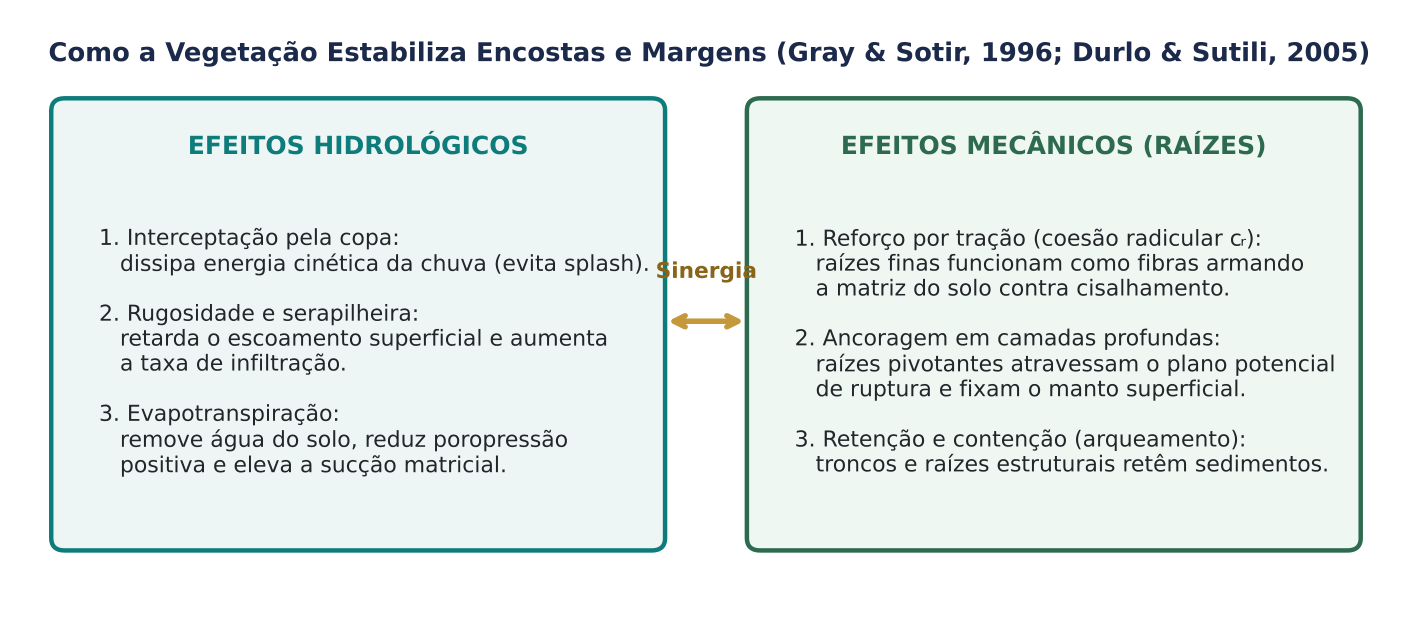
\includegraphics[keepaspectratio]{capitulos/../img/fig13_efeitos_raizes_solo.png}}

}

\caption{\label{fig-efeitos_raizes_solo}Integração dos efeitos mecânicos
(tração radicular, ancoragem em camadas estáveis e arqueamento lateral)
e efeitos hidrológicos (interceptação da copa, rugosidade superficial,
infiltração e evapotranspiração) da vegetação na estabilização de
encostas e margens.}

\end{figure}%

No plano mecânico, Gray e Sotir (1996) sistematizam três mecanismos
principais pelas quais as raízes estabilizam o solo,

\textbf{Reforço por tração radicular (\(\Delta c_r\)).} O solo possui
boa resistência à compressão, porém baixa resistência à tração. As
raízes finas e médias comportam-se como fibras flexíveis de alta
resistência à tração inseridas na matriz terrosa. Quando uma zona
potencial de cisalhamento tende a escorregar, as raízes que cruzam esse
plano são tensionadas e transferem parte do esforço para o solo
adjacente. \textbf{Ancoragem em horizontes firmes.} Raízes pivotantes
profundas atravessam horizontes superficiais mais friáveis ou alterados
e ancoram-se em camadas subsuperficiais mais coesas ou fraturas do
saprolito, atuando de modo análogo a microestacas naturais.

\textbf{Arqueamento e contenção lateral.} Sistemas radiculares densos de
árvores e arbustos distribuídos em encostas formam zonas de maior
rigidez que redistribuem tensões por efeito de arco, restringindo o
deslocamento de pequenas cunhas de solo entre os troncos.

No plano hidrológico, a vegetação promove quatro efeitos protetores
complementares, (1) \textbf{interceptação} da chuva pelas copas e pela
serapilheira, amortecendo a energia cinética das gotas antes do contato
com o solo; (2) aumento da \textbf{rugosidade superficial}, que reduz a
velocidade de escoamento laminar e concentrado; (3) estímulo à
\textbf{infiltração} via bioporos formados por raízes mortas e atividade
biológica; e (4) \textbf{evapotranspiração}, que consome água da zona
radicular, reduzindo o grau de saturação e a poropressão positiva
(\(u\)) no interior do talude entre eventos chuvosos.

\subsection{\texorpdfstring{Critério de Mohr-Coulomb com Reforço
Radicular
(\(\Delta c_r\))}{Critério de Mohr-Coulomb com Reforço Radicular (\textbackslash Delta c\_r)}}\label{13-bioengenharia-agua-solo-crituxe9rio-de-mohrcoulomb-com-reforuxe7o-radicular-delta-c_r}

Na mecânica dos solos clássica, a resistência ao cisalhamento \(\tau\)
de um solo saturado ou parcialmente saturado é expressa pela equação de
Mohr-Coulomb. Quando incorporamos a malha de raízes vivas, soma-se um
termo de coesão aparente radicular \(c_r\) (também grafado
\(\Delta c_r\)),

\[
\tau = (c' + c_r) + \sigma' \tan\phi'
\]

\textbf{Leitura intuitiva dos termos,}

\(c'\) é a ``cola'' natural entre as partículas minerais e orgânicas do
solo (coesão efetiva, em \(\text{kPa}\)); em solos arenosos puros,
\(c'\) aproxima-se de zero. \(c_r\) (\(\Delta c_r\)) é o reforço
adicional fornecido pelas raízes que atravessam o plano de ruptura (em
\(\text{kPa}\)), funcionando como uma armadura fibrosa distribuída
tridimensionalmente no solo superficial. \(\sigma'\) é a tensão normal
efetiva (\(\sigma' = \sigma - u\), onde \(\sigma\) é o peso da massa de
solo acima do plano e \(u\) é a pressão da água nos poros). Quanto menor
a poropressão \(u\) (graças à evapotranspiração e à drenagem adequada),
maior é \(\sigma'\) e maior é o atrito resistente \(\sigma'\tan\phi'\).

\(\phi'\) é o ângulo de atrito interno efetivo, que expressa o
intertravamento mecânico entre os grãos do solo.

\textbf{Fator de Segurança simplificado (\(FS\)).} Comparando a
resistência disponível \(\tau\) com a tensão cisalhante solicitante
\(\tau_{\text{sol}}\) exercida pelo peso da camada inclinada, tem-se
\(FS = \tau / \tau_{\text{sol}}\). Valores de \(FS < 1{,}0\) indicam
instabilidade; o ganho de \(c_r\) e a redução de \(u\) elevam \(FS\)
para patamares seguros.

\subsection{Técnicas Vegetativas, Paliçadas Permeáveis e Biomantas
Biodegradáveis}\label{tuxe9cnicas-vegetativas-paliuxe7adas-permeuxe1veis-e-biomantas-biodegraduxe1veis}

A seleção das técnicas de bioengenharia depende da declividade da
vertente, da presença de fluxo concentrado, da profundidade da incisão
erosiva e das condições climáticas locais. Em ambientes semiáridos, como
a área de estudo da disciplina CHF662 na Bahia, a escolha deve
considerar chuvas convectivas concentradas e longos períodos de déficit
hídrico.

\subsubsection{Técnicas vegetativas lineares e de cobertura, estacas
vivas, fascinas e
trançados}\label{tuxe9cnicas-vegetativas-lineares-e-de-cobertura-estacas-vivas-fascinas-e-tranuxe7ados}

\textbf{Estacas vivas (\emph{live stakes}),} segmentos lenhosos ou
semilenhosos de espécies com alta capacidade de brotação vegetativa
(como gliricídia, sabiá, salgueiro em áreas úmidas ou espécies nativas
propagáveis por estaquia), cravados perpendicularmente à superfície do
talude ou levemente inclinados para jusante. Atuam como pinos biológicos
que drenam e ancoram os primeiros \(0{,}4\text{ m}\) a
\(0{,}8\text{ m}\) de solo. \textbf{Fascinas vivas (\emph{live
fascines}),} feixes cilíndricos alongados de ramos vivos amarrados com
arame ou sisal, enterrados parcialmente em valas em curva de nível ao
longo da encosta ou na base de margens fluviais. As fascinas funcionam
como pequenos terraços permeáveis contínuos que quebram o comprimento de
rampa, retêm sedimentos finos e emitem raízes e brotos ao longo de todo
o feixe.

\textbf{Trançados vivos (\emph{wattle fences}),} cercas baixas
construídas com estacas cravadas verticalmente e ramos flexíveis
entrelaçados horizontalmente em curvas de nível. Retêm solo mobilizado a
montante e criam patamares de baixa declividade favoráveis ao
estabelecimento de mudas.

\subsubsection{Paliçadas e barragens permeáveis no controle de ravinas e
voçorocas}\label{paliuxe7adas-e-barragens-permeuxe1veis-no-controle-de-ravinas-e-vouxe7orocas}

Quando a erosão já formou sulcos profundos, ravinas ou voçorocas, apenas
técnicas de cobertura superficial não resistem ao fluxo concentrado.
Nesse cenário, implantam-se \textbf{paliçadas} (ou pequenas
\textbf{barragens permeáveis} de madeira, bambu, estacas vivas ou
sacaria biodegradável preenchida com solo local). Diferentemente de
barragens rígidas impermeáveis, a paliçada permite a passagem lenta da
água através dos interstícios, reduzindo o empuxo hidrostático, enquanto
retém as partículas sólidas transportadas por arraste e saltação.

\begin{figure}[H]

\centering{

\pandocbounded{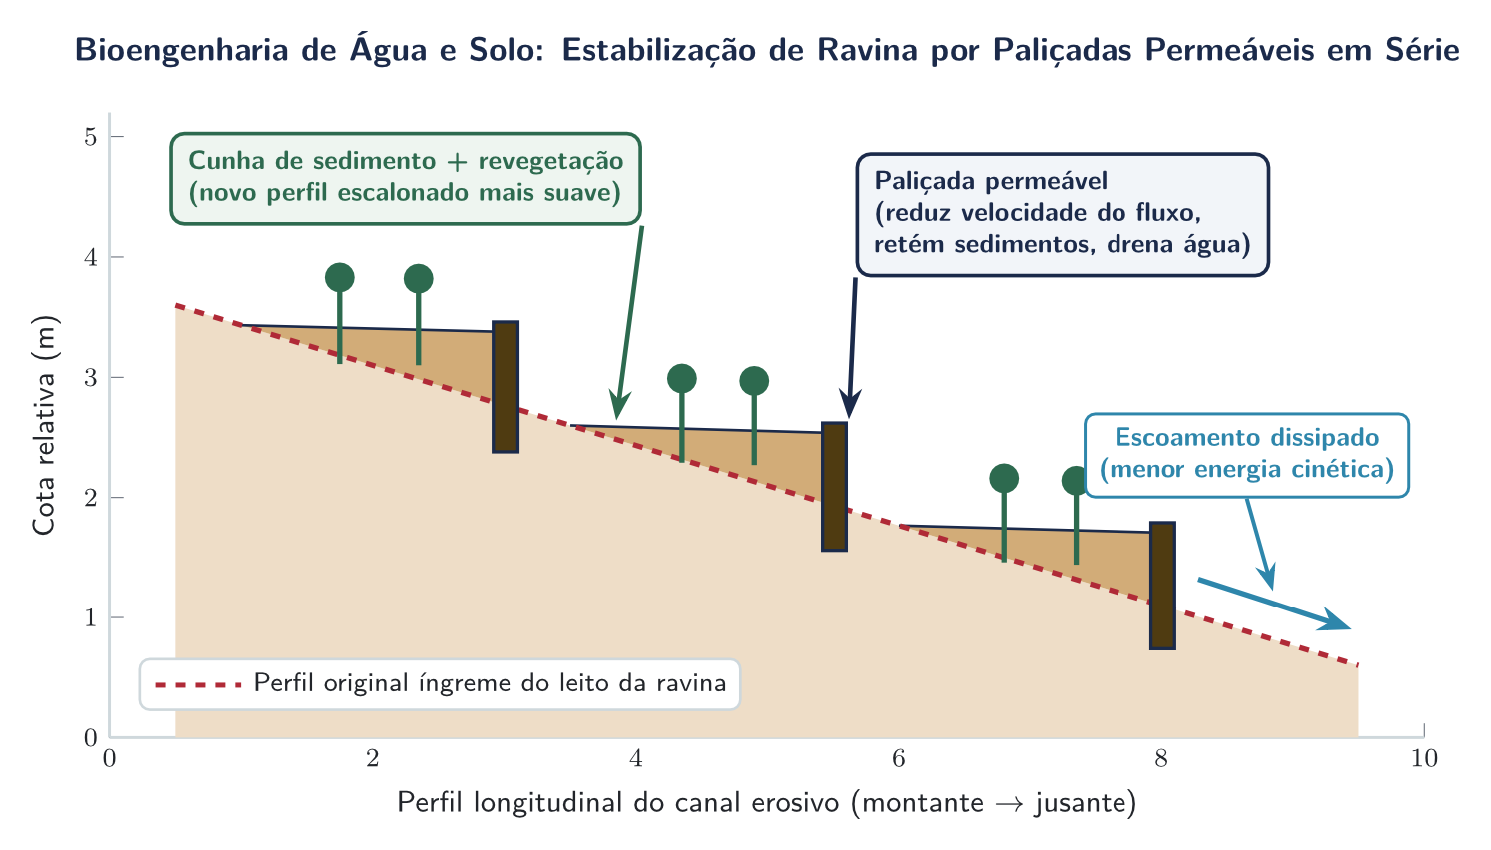
\includegraphics[keepaspectratio]{capitulos/../img/fig12_bioengenharia_palicada_talude.png}}

}

\caption{\label{fig-bioengenharia_palicada_talude}Esquema técnico de
controle de erosão linear com paliçadas permeáveis escalonadas em série,
evidenciando o espaçamento \(E = h/S\), a cunha de sedimentos retidos a
montante e o revestimento complementar de talude com biomanta e estacas
vivas.}

\end{figure}%

O acúmulo gradual de sedimentos a montante de cada paliçada reduz a
declividade do leito da ravina, formando patamares estabilizados
(degraus vegetados) que diminuem a velocidade da enxurrada e permitem a
colonização vegetal no interior da antiga incisão.

\subsection{\texorpdfstring{Dimensionamento de Paliçadas, Espaçamento
(\(E\)) e Cunha de Sedimentos
(\(V\))}{Dimensionamento de Paliçadas, Espaçamento (E) e Cunha de Sedimentos (V)}}\label{dimensionamento-de-paliuxe7adas-espauxe7amento-e-e-cunha-de-sedimentos-v}

Para que o sistema funcione em cascata, o pé de uma paliçada a montante
deve coincidir com o topo da cunha de sedimentos retida pela paliçada
imediatamente a jusante, nivelando o perfil do canal em degraus
estáveis,

\textbf{Espaçamento longitudinal entre paliçadas (\(E\)),}

\[
E = \frac{h}{S}
\]

onde \(h\) é a altura útil da paliçada acima do fundo do canal
(\(\text{m}\)) e \(S\) é a declividade longitudinal do leito em razão
decimal (\(\text{m}\cdot\text{m}^{-1}\); por exemplo, uma declividade de
\(10\%\) corresponde a \(S = 0{,}10\)). Em solos muito friáveis ou
curvas sinuosas, recomenda-se reduzir o espaçamento em \(15\%\) a
\(20\%\) por margem de segurança. \textbf{Estimativa do volume da cunha
de sedimentos retidos (\(V\)),} Considerando a cunha acumulada a
montante com seção longitudinal triangular de altura \(h\) na face da
paliçada, comprimento nivelado \(L_m\) (no limite teórico, \(L_m = E\))
e largura média do canal \(b\), o volume máximo retido por uma paliçada
é,

\[
V = \frac{1}{2} \cdot L_m \cdot h \cdot b
\]

onde \(V\) resulta em metros cúbicos (\(\text{m}^3\)). Multiplicando-se
\(V\) pela densidade aparente seca do sedimento (\(\rho_s\), em
\(\text{t}\cdot\text{m}^{-3}\)), obtém-se a massa de solo retida na
ravina (\(M = V \cdot \rho_s\)), impedindo que esse material alcance
cursos d'água e reservatórios a jusante.

\subsubsection{Biomantas, geotêxteis biodegradáveis e retentores de
sedimentos}\label{biomantas-geotuxeaxteis-biodegraduxe1veis-e-retentores-de-sedimentos}

Em taludes recém-conformados, platôs de obras lineares ou áreas
submetidas a hidrossemeadura, as \textbf{biomantas} e os
\textbf{geotêxteis biodegradáveis} oferecem proteção imediata ao solo
nu. São mantas tecidas ou costuradas com fibras vegetais naturais,

\textbf{Fibra de sisal (\emph{Agave sisalana}),} amplamente disponível
na Bahia, apresenta boa resistência mecânica inicial e decomposição
moderada (\(12\) a \(24\) meses), integrando-se à economia regional do
Semiárido. \textbf{Fibra de coco (\emph{Cocos nucifera}),} elevada
proporção de lignina, conferindo maior longevidade (\(24\) a \(48\)
meses), indicada para taludes íngremes e margens sujeitas a fluxo
intermitente mais energético. \textbf{Fibra de taboa (\emph{Typha
domingensis}) e juta,} materiais leves e altamente higroscópicos, úteis
para retenção de umidade em climas secos e proteção de superfícies de
baixa a média declividade até a germinação do estrato herbáceo.

Associam-se às biomantas os \textbf{retentores de sedimentos}
(biorretentores cilíndricos preenchidos com palha, fibra de coco ou
casca de arroz, dispostos em curvas de nível ou na base de taludes) e a
\textbf{revegetação estratificada}, que combina gramíneas de cobertura
rápida com leguminosas fixadoras de nitrogênio e espécies
arbustivo-arbóreas nativas.

\subsection{Quadro Comparativo, Bioengenharia vs.~Obras Cinzas
Rígidas}\label{quadro-comparativo-bioengenharia-vs.-obras-cinzas-ruxedgidas}

A escolha entre soluções baseadas na natureza e obras convencionais de
engenharia civil não deve ser ideológica, mas técnica. Em encostas com
risco geotécnico imediato sobre edificações críticas ou em gargantas
fluviais submetidas a velocidades hidráulicas extremas, estruturas
rígidas podem ser indispensáveis. Entretanto, na vasta maioria das áreas
degradadas rurais, faixas de domínio e margens fluviais, a bioengenharia
supera as obras cinzas em custo-efetividade e desempenho ecológico.

{\def\LTcaptype{none} % do not increment counter
\begin{longtable}[]{@{}
  >{\raggedright\arraybackslash}p{(\linewidth - 4\tabcolsep) * \real{0.3333}}
  >{\raggedright\arraybackslash}p{(\linewidth - 4\tabcolsep) * \real{0.3333}}
  >{\raggedright\arraybackslash}p{(\linewidth - 4\tabcolsep) * \real{0.3333}}@{}}
\toprule\noalign{}
\begin{minipage}[b]{\linewidth}\raggedright
\textbf{Critério de Análise}
\end{minipage} & \begin{minipage}[b]{\linewidth}\raggedright
\textbf{Bioengenharia de Água e Solo}
\end{minipage} & \begin{minipage}[b]{\linewidth}\raggedright
\textbf{Obras Cinzas Rígidas (Concreto / Alvenaria)}
\end{minipage} \\
\midrule\noalign{}
\endhead
\bottomrule\noalign{}
\endlastfoot
\textbf{Evolução do desempenho} & Crescente ao longo do tempo, à medida
que a vegetação se estabelece, aumenta a resistência radicular e a
cobertura. & Decrescente ao longo do tempo, sujeita a fissuras, fadiga
estrutural, desgaste hidráulico e solapamento sem autorreparação. \\
\textbf{Interação hidrológica} & Mantém a permeabilidade, favorece a
infiltração, alivia poropressões e reduz picos de cheia a jusante. &
Impermeabiliza o substrato, exige sistemas complexos de drenos e pode
transferir energia erosiva para jusante. \\
\textbf{Custo de implantação} & Reduzido (\(30\%\) a \(75\%\) menor em
taludes e ravinas), utilizando mão de obra e insumos vegetais locais. &
Elevado devido a escavações profundas, formas, aço, cimento e transporte
de materiais pesados. \\
\textbf{Manutenção inicial} & Maior atenção nos primeiros \(12\) a
\(24\) meses (irrigação de pegamento, replantio, controle de formigas).
& Baixa no curto prazo, porém reparos corretivos após trincas ou
recalques são complexos e onerosos. \\
\textbf{Valor ecológico e legal} & Restaura funções ecossistêmicas,
conectividade ripária e biodiversidade; atende diretamente metas de PRAD
em APPs. & Fragmenta habitats marginais, bloqueia trocas solo-água e
limita a regeneração da vegetação nativa. \\
\end{longtable}
}

\subsection{Escolha da técnica, implantação e
acompanhamento}\label{escolha-da-tuxe9cnica-implantauxe7uxe3o-e-acompanhamento}

Uma paliçada permeável instalada em um canal erosivo modifica a
velocidade e favorece deposição a montante. Seu desempenho depende do
escoamento que recebe, do apoio nas margens e da passagem controlada da
água. Desvios laterais e erosão no pé podem concentrar esforços em
pontos que precisam ser observados após os eventos de chuva.

O espaçamento geométrico calculado pela relação entre altura e
declividade constitui uma aproximação de organização longitudinal. A
implantação exige examinar vazão, geometria, fundação, estabilidade e
comportamento dos materiais. O cálculo didático de espaçamento deve ser
interpretado dentro dessas condições, com critérios de projeto definidos
para a situação real.

O estabelecimento vegetal acrescenta uma dimensão temporal.
Disponibilidade de água, período de plantio, adaptação da espécie e
proteção contra pastejo influenciam sobrevivência e cobertura. A
resistência de um material biodegradável também muda ao longo do tempo,
exigindo compatibilidade entre duração da proteção inicial e
desenvolvimento da vegetação.

O monitoramento deve registrar sobrevivência, cobertura, integridade dos
materiais, alteração da seção e manutenção após chuvas. A redução do
avanço erosivo precisa ser interpretada junto à chuva e às mudanças de
drenagem. Fotografias com posição repetida e medidas em referências
fixas ajudam a distinguir deposição temporária, estabilização e novos
caminhos de escoamento.

\subsection{Evidências experimentais para a escolha de materiais de
proteção}\label{eviduxeancias-experimentais-para-a-escolha-de-materiais-de-proteuxe7uxe3o}

A proteção de uma superfície depende da continuidade do contato entre
material, solo e vegetação (Figura~\ref{fig-geocomposito-estrutura}). O
geocompósito multicamada do estudo fornecido por Santos e colaboradores
permite observar a organização das fibras e sua interface com o terreno.
A inspeção dessa interface ajuda a reconhecer caminhos de água sob o
material, descolamentos e perda de contato durante a exposição.

\begin{figure}[H]

\centering{

\pandocbounded{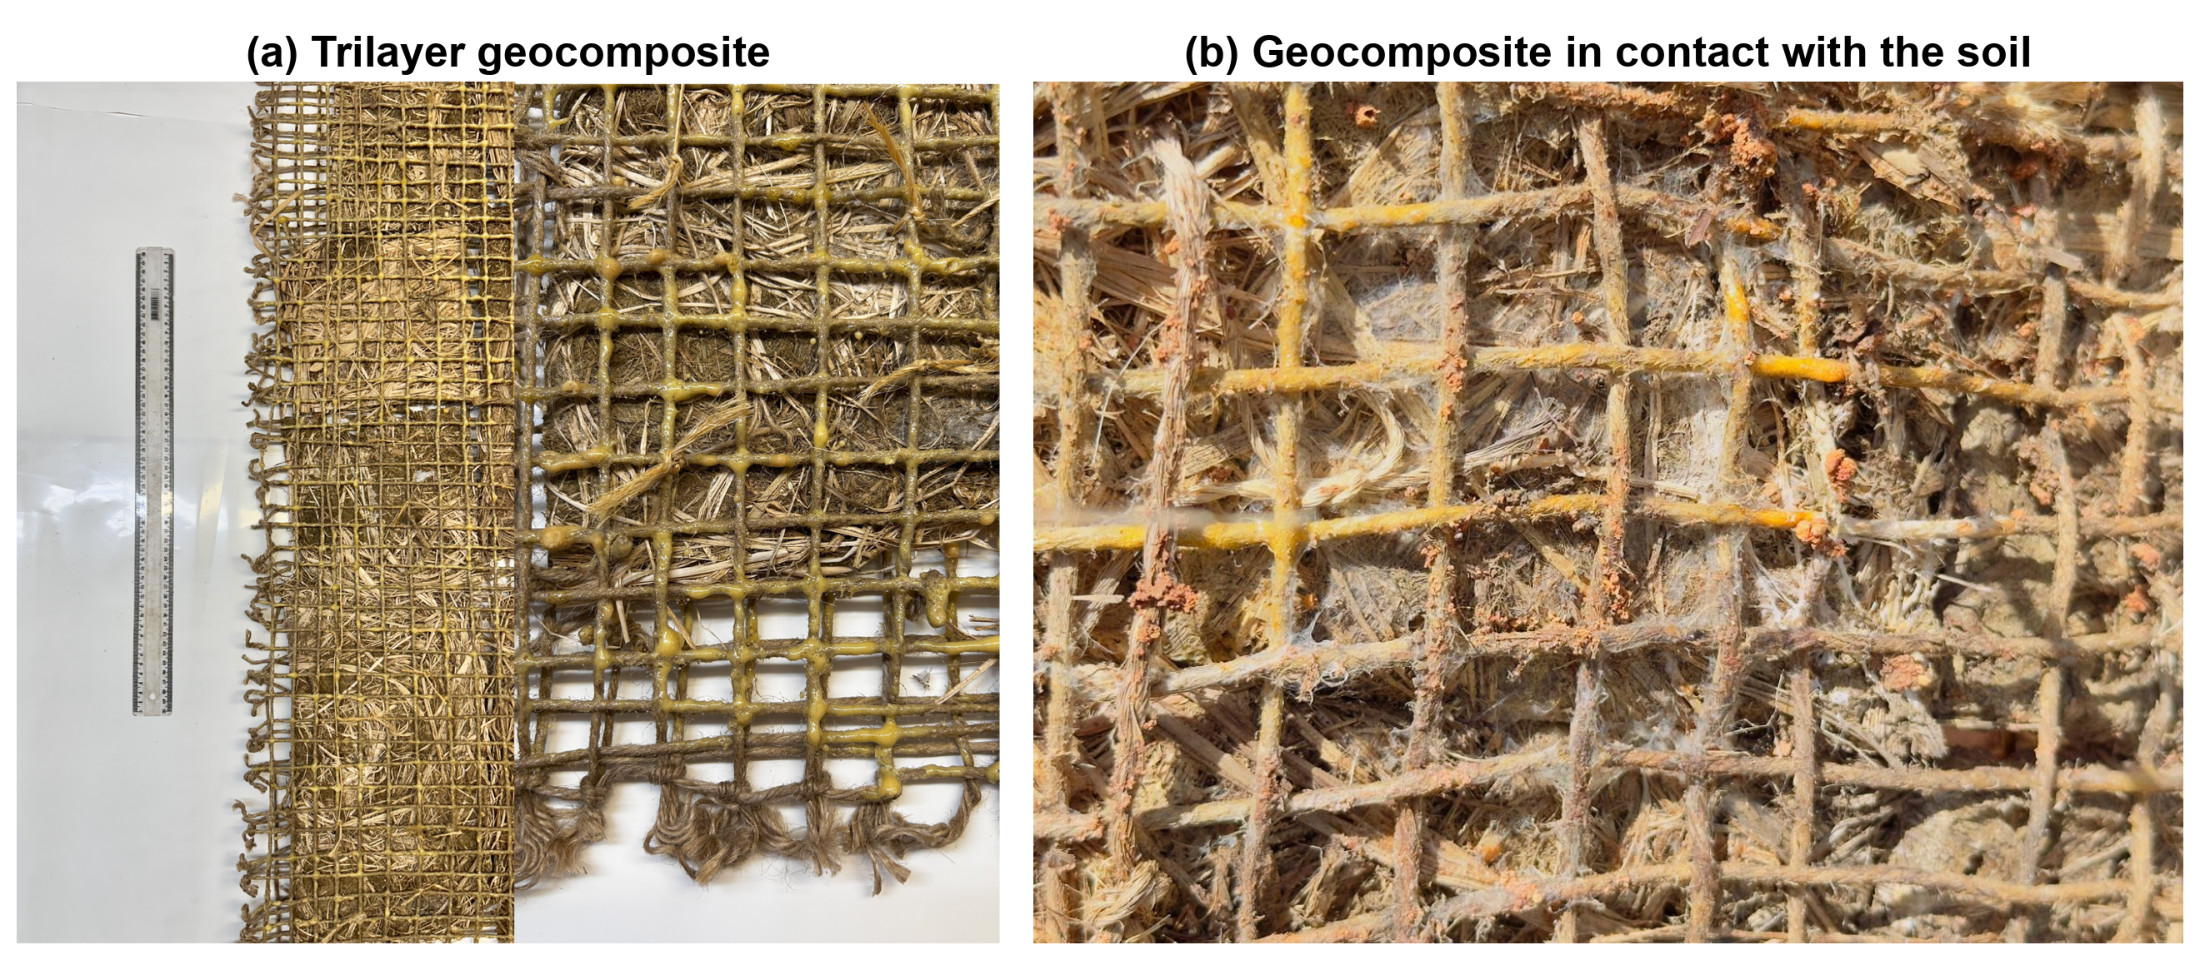
\includegraphics[keepaspectratio,alt={Painel com a organização das camadas de fibras do geocompósito e detalhe do material em contato com o solo}]{capitulos/../img/artigo_geocomposito_estrutura.jpg}}

}

\caption{\label{fig-geocomposito-estrutura}Estrutura de um geocompósito
multicamada e contato com o solo. Fonte Santos e colaboradores,
manuscrito sobre degradação em campo e confiabilidade mecânica de
geocompósito de fibras naturais, acervo fornecido pelo autor. Reprodução
sem alteração.}

\end{figure}%

O arranjo experimental apresenta parcelas delimitadas, materiais e
coletores que permitem relacionar as condições de exposição aos
resultados de campo (Figura~\ref{fig-geocomposito-campo}). A comparação
entre tratamentos exige conhecer suas dimensões, réplicas, período de
acompanhamento e procedimentos de coleta. As fotografias documentam o
método, enquanto a avaliação de desempenho depende dos dados
correspondentes.

\begin{figure}[H]

\centering{

\pandocbounded{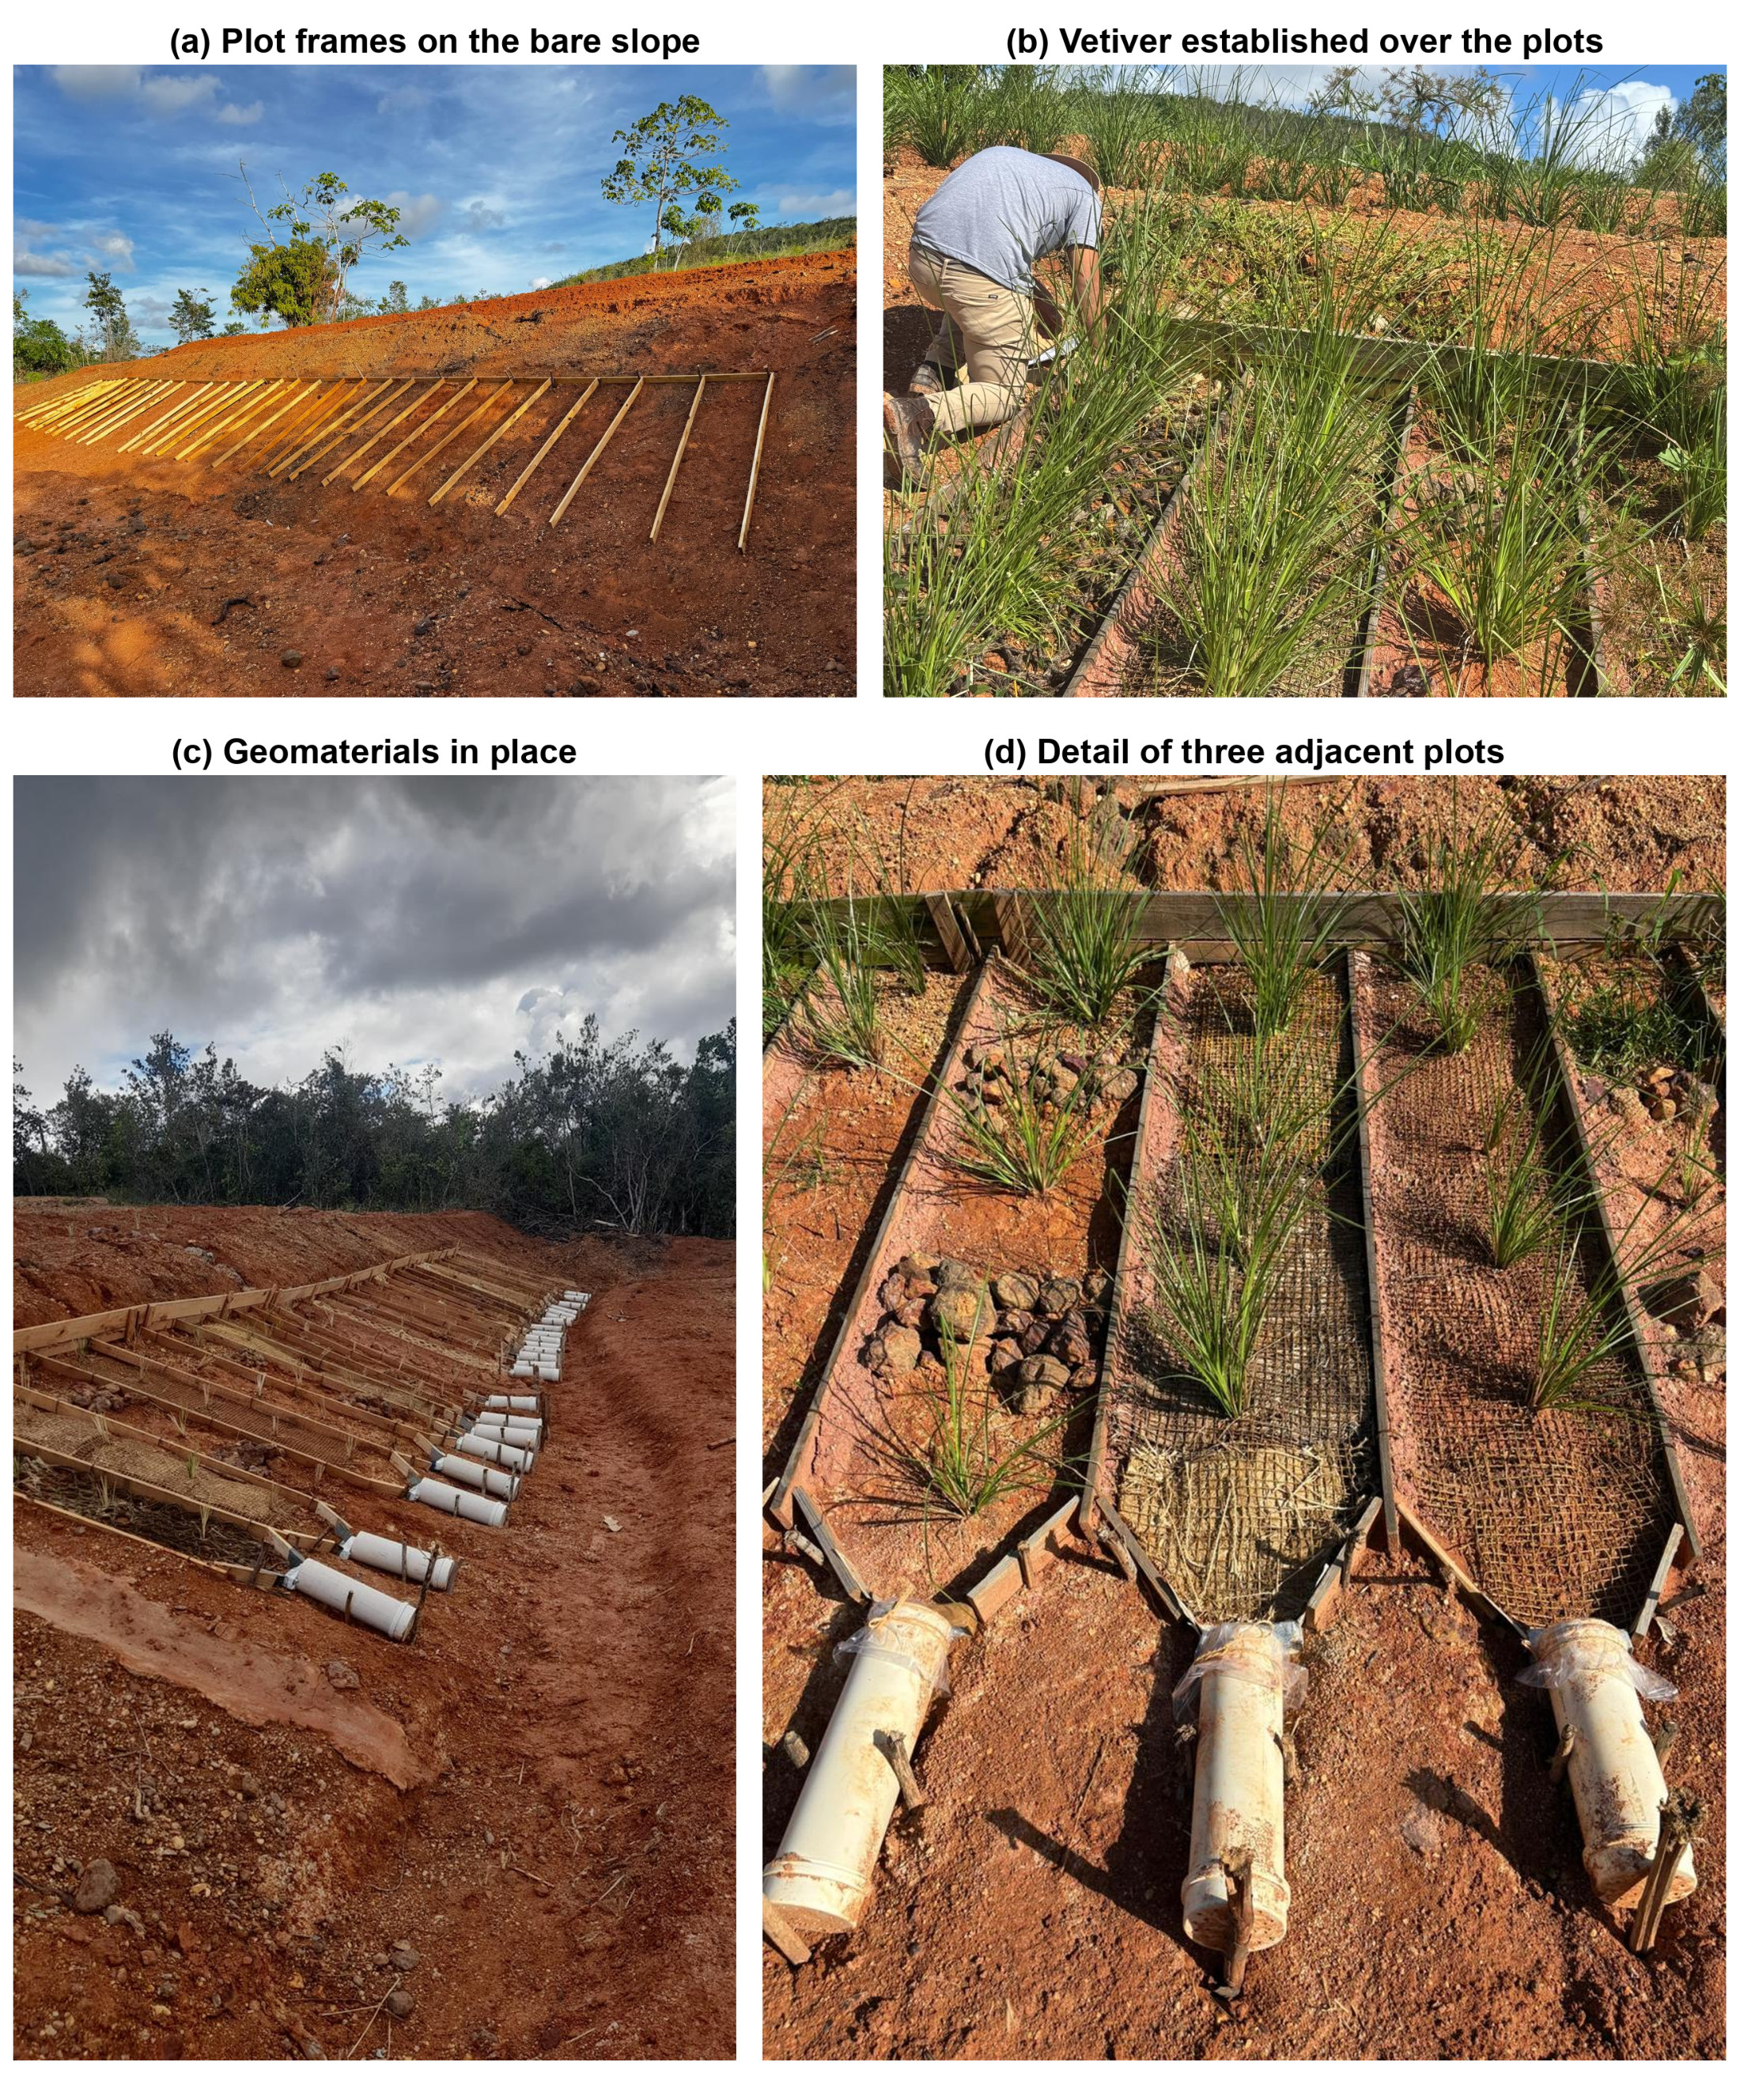
\includegraphics[keepaspectratio,alt={Quatro fotografias de parcelas em talude, vegetação de vetiver, geomateriais e coletores na base das parcelas}]{capitulos/../img/artigo_geocomposito_campo.jpg}}

}

\caption{\label{fig-geocomposito-campo}Implantação e acompanhamento de
parcelas com geomateriais e vetiver. Fonte Santos e colaboradores,
manuscrito sobre degradação de geocompósito em condições tropicais,
acervo fornecido pelo autor. As letras dos painéis e o idioma da figura
original foram mantidos.}

\end{figure}%

A convergência com o diagnóstico da disciplina ocorre na escolha das
variáveis que permitem acompanhar o funcionamento. Integridade do
material, cobertura vegetal e sobrevivência descrevem o estado da
intervenção. Volume e massa coletados, quando medidos com protocolo e
referência de chuva, permitem examinar sua resposta
hidrossedimentológica. Ensaios de tração e punção acrescentam informação
sobre resistência e duração, cuja interpretação deve acompanhar
unidades, dimensões dos corpos de prova e variabilidade.

A transferência para taludes de acessos, margens ou áreas degradadas
depende de compatibilidade entre solo, declividade, energia do
escoamento e disponibilidade hídrica. Uma superfície com fluxo
distribuído e uma margem submetida a ondas recebem solicitações
diferentes. A seleção de um material deve explicar como essas
solicitações serão atendidas durante o período necessário ao
estabelecimento vegetal.

\section{Etapa 4 - Exemplos
resolvidos}\label{etapa-4---exemplos-resolvidos-12}

\subsection{Exemplo 1. Reforço Radicular na Equação de Mohr-Coulomb em
Talude
Degradado}\label{13-bioengenharia-agua-solo-exemplo-1.-reforuxe7o-radicular-na-equauxe7uxe3o-de-mohrcoulomb-em-talude-degradado}

\textbf{Situação analisada.} Durante o diagnóstico de um talude de corte
em solo argilo-arenoso ao longo de uma estrada de acesso no Semiárido
Baiano, avalia-se o ganho de estabilidade proporcionado pela implantação
de vegetação de enraizamento denso em comparação ao solo exposto.

\textbf{Dados disponíveis.} Coesão efetiva do solo
\(c' = 8{,}0\text{ kPa}\); ângulo de atrito efetivo \(\phi' = 28^\circ\)
(\(\tan 28^\circ \approx 0{,}5317\)); tensão normal efetiva no plano
potencial de ruptura \(\sigma' = 25{,}0\text{ kPa}\); reforço radicular
medido para a espécie implantada \(c_r = 6{,}5\text{ kPa}\); tensão
cisalhante solicitante durante chuva intensa
\(\tau_{\text{sol}} = 23{,}0\text{ kPa}\).

\textbf{Problema a resolver.} Calcule a resistência ao cisalhamento sem
vegetação (\(\tau_0\)) e com vegetação (\(\tau_1\)), o ganho percentual
de resistência e o Fator de Segurança
(\(FS = \tau / \tau_{\text{sol}}\)) nos dois cenários.

\textbf{Fundamento da análise.} Aplicação direta do critério de
Mohr-Coulomb modificado pelo reforço radicular (Gray; Sotir, 1996),
\(\tau = (c' + c_r) + \sigma'\tan\phi'\).

\textbf{Desenvolvimento.} 1. Parcela de atrito interno do solo,

\[
\sigma' \tan\phi' = 25{,}0 \times 0{,}5317 = 13{,}29\text{ kPa}
\]

\begin{enumerate}
\def\labelenumi{\arabic{enumi}.}
\setcounter{enumi}{1}
\tightlist
\item
  Resistência ao cisalhamento sem raízes (\(c_r = 0\)),
\end{enumerate}

\[
\tau_0 = 8{,}0 + 13{,}29 = 21{,}29\text{ kPa}
\]

\begin{enumerate}
\def\labelenumi{\arabic{enumi}.}
\setcounter{enumi}{2}
\tightlist
\item
  Resistência ao cisalhamento com reforço radicular
  (\(c_r = 6{,}5\text{ kPa}\)),
\end{enumerate}

\[
\tau_1 = (8{,}0 + 6{,}5) + 13{,}29 = 14{,}5 + 13{,}29 = 27{,}79\text{ kPa}
\]

\begin{enumerate}
\def\labelenumi{\arabic{enumi}.}
\setcounter{enumi}{3}
\tightlist
\item
  Ganho percentual de resistência,
\end{enumerate}

\[
\Delta_{\%} = \frac{27{,}79 - 21{,}29}{21{,}29} \times 100\% = \frac{6{,}50}{21{,}29} \times 100\% \approx 30{,}53\%
\]

\begin{enumerate}
\def\labelenumi{\arabic{enumi}.}
\setcounter{enumi}{4}
\tightlist
\item
  Cálculo do Fator de Segurança (\(FS\)),
\end{enumerate}

\[
FS_0 = \frac{21{,}29}{23{,}0} \approx 0{,}93 \quad (\text{instável, } FS < 1{,}0)
\]

\[
FS_1 = \frac{27{,}79}{23{,}0} \approx 1{,}21 \quad (\text{estável, } FS > 1{,}0)
\]

\textbf{Interpretação do resultado.} Sem vegetação,
\(\tau_0 = 21{,}29\text{ kPa}\) (\(FS_0 = 0{,}93\)); com reforço
radicular, \(\tau_1 = 27{,}79\text{ kPa}\) (\(FS_1 = 1{,}21\)),
representando ganho de \(30{,}53\%\) na resistência ao cisalhamento.

\textbf{Condições de validade.} O resultado é coerente com a física do
solo, um incremento modesto de coesão radicular (\(6{,}5\text{ kPa}\)) é
suficiente para converter um talude superficialmente instável
(\(FS < 1{,}0\)) em estável (\(FS > 1{,}2\)) sob condição chuvosa
crítica.

\subsection{Exemplo 2. Dimensionamento de Paliçadas Permeáveis e Volume
de Sedimentos
Retidos}\label{exemplo-2.-dimensionamento-de-paliuxe7adas-permeuxe1veis-e-volume-de-sedimentos-retidos}

\textbf{Situação analisada.} Uma ravina ativa formada a jusante de um
bueiro rodoviário apresenta risco de evoluir para voçoroca e assorear um
riacho intermitente. A equipe técnica propõe instalar paliçadas de
madeira e bambu em série ao longo do trecho mais íngreme.

\textbf{Dados disponíveis.} Comprimento total do trecho a tratar
\(L_t = 45{,}0\text{ m}\); declividade longitudinal média do leito da
ravina \(S = 8\%\) (\(0{,}08\text{ m}\cdot\text{m}^{-1}\)); altura útil
adotada para cada paliçada \(h = 0{,}60\text{ m}\); largura média da
seção da ravina \(b = 2{,}50\text{ m}\); densidade aparente do sedimento
retido \(\rho_s = 1{,}35\text{ t}\cdot\text{m}^{-3}\).

\textbf{Problema a resolver.} Determine o espaçamento teórico entre
paliçadas (\(E\)), a quantidade de estruturas necessárias no trecho
(\(n\)), o volume da cunha de sedimentos retido por paliçada (\(V_1\)),
o volume total (\(V_{\text{total}}\)) e a massa total de sedimentos
retida (\(M\)).

\textbf{Fundamento da análise.} Cálculo geométrico de perfil nivelado em
degraus (\(E = h/S\)) e volume prismático triangular de cunha sedimentar
(\(V = \frac{1}{2}\cdot L_m \cdot h \cdot b\), com \(L_m = E\)).

\textbf{Desenvolvimento.} 1. Espaçamento longitudinal entre paliçadas,

\[
E = \frac{h}{S} = \frac{0{,}60}{0{,}08} = 7{,}50\text{ m}
\]

\begin{enumerate}
\def\labelenumi{\arabic{enumi}.}
\setcounter{enumi}{1}
\tightlist
\item
  Número de paliçadas ao longo dos \(45{,}0\text{ m}\),
\end{enumerate}

\[
n = \frac{L_t}{E} = \frac{45{,}0}{7{,}50} = 6\text{ paliçadas}
\]

\begin{enumerate}
\def\labelenumi{\arabic{enumi}.}
\setcounter{enumi}{2}
\tightlist
\item
  Volume da cunha de sedimentos retida por uma paliçada
  (\(L_m = E = 7{,}50\text{ m}\)),
\end{enumerate}

\[
V_1 = \frac{1}{2} \cdot L_m \cdot h \cdot b = 0{,}5 \times 7{,}50 \times 0{,}60 \times 2{,}50 = 5{,}625\text{ m}^3
\]

\begin{enumerate}
\def\labelenumi{\arabic{enumi}.}
\setcounter{enumi}{3}
\tightlist
\item
  Volume total e massa de sedimentos retidos pelo sistema completo,
\end{enumerate}

\[
V_{\text{total}} = 6 \times 5{,}625 = 33{,}75\text{ m}^3
\]

\[
M = V_{\text{total}} \cdot \rho_s = 33{,}75 \times 1{,}35 = 45{,}56\text{ t}
\]

\textbf{Interpretação do resultado.} Espaçamento
\(E = 7{,}50\text{ m}\); \(n = 6\) paliçadas;
\(V_1 = 5{,}625\text{ m}^3\) por estrutura; volume total retido
\(V_{\text{total}} = 33{,}75\text{ m}^3\), equivalente a
\(45{,}56\text{ t}\) de sedimentos.

\textbf{Condições de validade.} Seis estruturas de \(0{,}60\text{ m}\)
de altura acumulam um desnível total de
\(6 \times 0{,}60 = 3{,}60\text{ m}\), exatamente igual ao desnível
natural do trecho de \(45{,}0\text{ m}\) a \(8\%\)
(\(45{,}0 \times 0{,}08 = 3{,}60\text{ m}\)), confirmando o fechamento
geométrico do escalonamento.

\subsection{Exemplo 3. Proteção Superficial com Biomanta de Sisal e
Redução de Perda de
Solo}\label{exemplo-3.-proteuxe7uxe3o-superficial-com-biomanta-de-sisal-e-reduuxe7uxe3o-de-perda-de-solo}

\textbf{Situação analisada.} Um talude de corte recém-terraplenado em um
empreendimento eólico no Semiárido apresenta perda de solo acentuada nos
primeiros meses chuvosos. Para conter a erosão laminar e viabilizar o
estabelecimento de gramíneas e leguminosas, prescreve-se a aplicação de
biomanta de fibra de sisal associada à hidrossemeadura.

\textbf{Dados disponíveis.} Área do talude \(A = 1.200\text{ m}^2\)
(\(0{,}12\text{ ha}\)); taxa de perda de solo sem proteção medida por
pinos de erosão igual a
\(45{,}0\text{ t}\cdot\text{ha}^{-1}\cdot\text{ano}^{-1}\); eficiência
de redução da perda de solo pela biomanta de sisal igual a \(85\%\);
dimensões comerciais do rolo de biomanta,
\(2{,}0\text{ m} \times 25{,}0\text{ m}\) (\(50{,}0\text{ m}^2\) por
rolo), exigindo \(10\%\) de acréscimo de área para sobreposição das
emendas.

\textbf{Problema a resolver.} Calcule a perda anual de solo sem proteção
e com biomanta (em \(\text{t}\cdot\text{ano}^{-1}\)), a massa de solo
retida anualmente na encosta e o número mínimo inteiro de rolos de
biomanta a adquirir.

\textbf{Fundamento da análise.} Conversão de área para hectares,
aplicação do fator de atenuação erosiva (\(1 - 0{,}85 = 0{,}15\)) e
dimensionamento de cobertura com sobreposição.

\textbf{Desenvolvimento.} 1. Perda anual sem proteção na área de
\(0{,}12\text{ ha}\),

\[
P_0 = 0{,}12\text{ ha} \times 45{,}0\text{ t}\cdot\text{ha}^{-1}\cdot\text{ano}^{-1} = 5{,}40\text{ t}\cdot\text{ano}^{-1}
\]

\begin{enumerate}
\def\labelenumi{\arabic{enumi}.}
\setcounter{enumi}{1}
\tightlist
\item
  Perda anual residual com biomanta (\(15\%\) da perda original),
\end{enumerate}

\[
P_1 = 5{,}40 \times (1 - 0{,}85) = 5{,}40 \times 0{,}15 = 0{,}81\text{ t}\cdot\text{ano}^{-1}
\]

\begin{enumerate}
\def\labelenumi{\arabic{enumi}.}
\setcounter{enumi}{2}
\tightlist
\item
  Massa de solo retida na encosta pela proteção,
\end{enumerate}

\[
\Delta P = 5{,}40 - 0{,}81 = 4{,}59\text{ t}\cdot\text{ano}^{-1}
\]

\begin{enumerate}
\def\labelenumi{\arabic{enumi}.}
\setcounter{enumi}{3}
\tightlist
\item
  Área efetiva de biomanta com \(10\%\) de sobreposição e número de
  rolos,
\end{enumerate}

\[
A_{\text{ef}} = 1.200 \times 1{,}10 = 1.320\text{ m}^2
\]

\[
N_{\text{rolos}} = \frac{1.320}{50{,}0} = 26{,}4 \rightarrow \mathbf{27\text{ rolos}}
\]

\textbf{Interpretação do resultado.} A perda cai de
\(5{,}40\text{ t}\cdot\text{ano}^{-1}\) para
\(0{,}81\text{ t}\cdot\text{ano}^{-1}\) (retenção de
\(4{,}59\text{ t}\cdot\text{ano}^{-1}\)); devem ser adquiridos \(27\)
rolos de biomanta de sisal.

\textbf{Condições de validade.} O arredondamento para cima (\(27\)
rolos) garante que não falte material nas bordas de ancoragem em valas
de coroamento e pé de talude, prática obrigatória em especificações
executivas.

\subsection{Exemplo 4. Dimensionamento de Estacas Vivas e Fascinas em
Margem
Fluvial}\label{exemplo-4.-dimensionamento-de-estacas-vivas-e-fascinas-em-margem-fluvial}

\textbf{Situação analisada.} Um trecho de margem fluvial degradada
apresenta solapamento na base e exposição do talude marginal. O projeto
de recuperação combina fascinas vivas na zona de variação do nível
d'água com plantio de estacas vivas na rampa superior.

\textbf{Dados disponíveis.} Extensão da margem \(L = 180\text{ m}\);
largura da faixa de rampa tratada com estacas vivas
\(w = 4{,}0\text{ m}\) (área \(= 720\text{ m}^2\)); espaçamento das
estacas na rampa igual a \(0{,}80\text{ m} \times 0{,}80\text{ m}\)
(\(0{,}64\text{ m}^2\) por estaca); \(3\) linhas contínuas de fascinas
na base (\(3 \times 180 = 540\text{ m}\) lineares), fixadas por \(1\)
estaca a cada \(0{,}75\text{ m}\); taxa média de pegamento esperada em
campo igual a \(75\%\).

\textbf{Problema a resolver.} Calcule o número de estacas na rampa, o
número de estacas de fixação das fascinas, o total de estacas
necessárias e a quantidade estimada de plantas vivas estabelecidas após
o primeiro ciclo chuvoso.

\textbf{Fundamento da análise.} Razão entre área/comprimento e
espaçamento unitário, seguida de aplicação da taxa de sobrevivência.

\textbf{Desenvolvimento.} 1. Estacas vivas distribuídas na rampa
(\(720\text{ m}^2\)),

\[
N_{\text{rampa}} = \frac{720}{0{,}64} = 1.125\text{ estacas}
\]

\begin{enumerate}
\def\labelenumi{\arabic{enumi}.}
\setcounter{enumi}{1}
\tightlist
\item
  Estacas de ancoragem ao longo dos \(540\text{ m}\) de fascinas,
\end{enumerate}

\[
N_{\text{fasc}} = \frac{540}{0{,}75} = 720\text{ estacas}
\]

\begin{enumerate}
\def\labelenumi{\arabic{enumi}.}
\setcounter{enumi}{2}
\tightlist
\item
  Total de estacas a produzir/colher,
\end{enumerate}

\[
N_{\text{total}} = 1.125 + 720 = 1.845\text{ estacas}
\]

\begin{enumerate}
\def\labelenumi{\arabic{enumi}.}
\setcounter{enumi}{3}
\tightlist
\item
  Estimativa de indivíduos vivos estabelecidos (\(75\%\) de pegamento),
\end{enumerate}

\[
N_{\text{vivas}} = 1.845 \times 0{,}75 = 1.383{,}75 \approx 1.384\text{ plantas vivas}
\]

\textbf{Interpretação do resultado.} São necessárias \(1.125\) estacas
na rampa e \(720\) nas fascinas (total de \(1.845\) estacas), resultando
em aproximadamente \(1.384\) plantas vivas estabelecidas.

\textbf{Condições de validade.} Mesmo com \(25\%\) de mortalidade
inicial, permanecem cerca de \(1{,}17\text{ planta}\cdot\text{m}^{-2}\)
na rampa (\(844/720\)) e \(3{,}0\text{ estacas}\cdot\text{m}^{-1}\) nas
fascinas ao longo da margem (\(540/180\)), densidades adequadas para
formar cobertura contínua na zona crítica.

\subsection{Exemplo 5. Análise Comparativa de Custo e Desempenho,
Bioengenharia vs.~Obra
Cinza}\label{exemplo-5.-anuxe1lise-comparativa-de-custo-e-desempenho-bioengenharia-vs.-obra-cinza}

\textbf{Situação analisada.} A prefeitura de um município baiano precisa
estabilizar \(100\text{ m}\) de talude marginal de uma estrada vicinal
que dá acesso a uma área de captação de água, evitando o assoreamento do
manancial.

\textbf{Dados disponíveis.} Extensão do trecho \(L = 100\text{ m}\);
altura do talude \(h = 3{,}0\text{ m}\). Alternativa A (obra cinza
rígida em muro de concreto/gabião argamassado), custo unitário de
\(\text{R\$ }1.850{,}00\cdot\text{m}^{-1}\). Alternativa B
(bioengenharia com retentores de sedimentos na base, biomanta de coco e
estacas vivas nativas), custo de implantação de
\(\text{R\$ }420{,}00\cdot\text{m}^{-1}\) mais plano de manutenção de
\(2\) anos orçado em \(\text{R\$ }8.000{,}00\) no total.

\textbf{Problema a resolver.} Calcule o custo total de cada alternativa,
a economia financeira absoluta e percentual proporcionada pela
bioengenharia e justifique a escolha sob a ótica hidrogeomorfológica.

\textbf{Fundamento da análise.} Orçamentação linear direta e comparação
relativa de custos associada à análise de serviços ecossistêmicos.

\textbf{Desenvolvimento.} 1. Custo total da Alternativa A (obra cinza),

\[
C_A = 100 \times 1.850{,}00 = \text{R\$ }185.000{,}00
\]

\begin{enumerate}
\def\labelenumi{\arabic{enumi}.}
\setcounter{enumi}{1}
\tightlist
\item
  Custo total da Alternativa B (bioengenharia + 2 anos de manutenção),
\end{enumerate}

\[
C_B = (100 \times 420{,}00) + 8.000{,}00 = 42.000{,}00 + 8.000{,}00 = \text{R\$ }50.000{,}00
\]

\begin{enumerate}
\def\labelenumi{\arabic{enumi}.}
\setcounter{enumi}{2}
\tightlist
\item
  Economia financeira absoluta e percentual,
\end{enumerate}

\[
\Delta C = 185.000{,}00 - 50.000{,}00 = \text{R\$ }135.000{,}00
\]

\[
\Delta C_{\%} = \frac{135.000{,}00}{185.000{,}00} \times 100\% \approx 72{,}97\%
\]

\textbf{Interpretação do resultado.} Alternativa A,
\(\text{R\$ }185.000{,}00\); Alternativa B, \(\text{R\$ }50.000{,}00\).
A bioengenharia gera economia de \(\text{R\$ }135.000{,}00\)
(\(72{,}97\%\)), além de preservar a infiltração na zona de recarga do
manancial.

\textbf{Condições de validade.} O valor de economia de \(72{,}97\%\) é
compatível com a literatura de Engenharia Natural para taludes de média
altura (\(3{,}0\text{ m}\)) sem cargas estruturais de edificações no
coroamento.

\section{Etapa 5 - Erros de
interpretação}\label{etapa-5---erros-de-interpretauxe7uxe3o-12}

\subsection{Erro 1, Construir Paliçadas Impermeáveis Sem Dissipação de
Energia}\label{erro-1-construir-paliuxe7adas-impermeuxe1veis-sem-dissipauxe7uxe3o-de-energia}

Fechar totalmente a seção da ravina com chapas rígidas, alvenaria sem
drenos ou lonas plásticas cria empuxo hidrostático excessivo a montante
e transbordamento concentrado pelas laterais, provocando erosão
regressiva nas ombreiras e destruição da obra logo na primeira enxurrada
intensa. Paliçadas devem ser \textbf{permeáveis} e devidamente
engastadas nas paredes laterais da ravina.

\subsection{Erro 2, Aplicar Biomanta Sem Contato Íntimo com o Solo
Preparado}\label{erro-2-aplicar-biomanta-sem-contato-uxedntimo-com-o-solo-preparado}

Estender biomantas sobre superfície irregular cheia de torrões, pedras
soltas ou sulcos não regularizados deixa bolsões de ar sob a manta. A
água da chuva escoa por baixo da biomanta, escava o solo invisivelmente
e impede que as raízes das sementes germinadas alcancem o substrato
mineral. O preparo, a regularização e o grampeamento firme ao solo são
obrigatórios.

\subsection{Erro 3, Usar Espécies Exóticas Invasoras por Facilidade de
Pegamento}\label{erro-3-usar-espuxe9cies-exuxf3ticas-invasoras-por-facilidade-de-pegamento}

Selecionar espécies exóticas agressivas (como leucena ou gramíneas
africanas invasoras) apenas pelo crescimento rápido compromete a
sucessão ecológica nativa e viola diretrizes de PRAD em Áreas de
Preservação Permanente. A escolha deve priorizar espécies nativas
regionais ou coberturas anuais não invasoras que cedam espaço às
nativas.

\subsection{Erro 4, Ignorar o Esforço de Manutenção Pós-Plantio no
Semiárido}\label{erro-4-ignorar-o-esforuxe7o-de-manutenuxe7uxe3o-puxf3s-plantio-no-semiuxe1rido}

Em regiões de baixa pluviosidade irregular, abandonar estacas, mudas ou
biomantas sem controle de formigas cortadeiras, proteção contra pisoteio
de rebanhos e irrigação de salvamento nos primeiros meses leva a taxas
de mortalidade superiores a \(80\%\), anulando o investimento inicial
antes que o reforço radicular \(c_r\) se estabeleça.

\section{Etapa 6 - Exercícios de
fixação}\label{etapa-6---exercuxedcios-de-fixauxe7uxe3o-12}

\subsubsection{Bloco A, Questões Conceituais Básicas (1 a
5)}\label{bloco-a-questuxf5es-conceituais-buxe1sicas-1-a-5}

\begin{enumerate}
\def\labelenumi{\arabic{enumi}.}
\item
  Explique o princípio da substituição gradual de funções entre
  materiais inertes biodegradáveis e elementos vivos na Bioengenharia de
  Solos.
\item
  Diferencie o papel mecânico do reforço por tração radicular (\(c_r\))
  do mecanismo de ancoragem profunda das raízes em uma encosta
  inclinada.
\item
  Descreva três efeitos hidrológicos da vegetação que contribuem para
  aumentar a estabilidade de um talude e reduzir o escoamento
  superficial.
\item
  Compare as finalidades construtivas de estacas vivas, fascinas e
  trançados vivos na recuperação de vertentes degradadas.
\item
  Cite três vantagens ambientais e econômicas das biomantas de fibra de
  sisal ou coco em comparação com o revestimento rígido em concreto
  projetado.
\end{enumerate}

\subsubsection{Bloco B, Questões Intermediárias e Quantitativas (6 a
10)}\label{bloco-b-questuxf5es-intermediuxe1rias-e-quantitativas-6-a-10}

\begin{enumerate}
\def\labelenumi{\arabic{enumi}.}
\setcounter{enumi}{5}
\item
  Um solo apresenta coesão efetiva \(c' = 6{,}0\text{ kPa}\), tensão
  normal efetiva \(\sigma' = 20{,}0\text{ kPa}\) e
  \(\tan\phi' = 0{,}50\). Calcule a resistência ao cisalhamento sem
  vegetação (\(\tau_0\)) e com reforço radicular
  \(c_r = 5{,}0\text{ kPa}\) (\(\tau_1\)), indicando o ganho percentual
  obtido.
\item
  Uma ravina com declividade longitudinal
  \(S = 0{,}10\text{ m}\cdot\text{m}^{-1}\) (\(10\%\)) será estabilizada
  com paliçadas de madeira de altura útil \(h = 0{,}50\text{ m}\) e
  largura média \(b = 2{,}00\text{ m}\). Calcule o espaçamento teórico
  \(E\) entre as paliçadas e o volume de sedimentos retido na cunha de
  uma paliçada (\(L_m = E\)).
\item
  Em um trecho de \(36{,}0\text{ m}\) de uma voçoroca com declividade
  \(S = 0{,}05\text{ m}\cdot\text{m}^{-1}\), deseja-se instalar
  paliçadas com altura útil \(h = 0{,}45\text{ m}\) e largura média
  \(b = 1{,}80\text{ m}\). Determine o espaçamento \(E\), o número de
  paliçadas necessárias e a massa total de sedimentos retida
  considerando \(\rho_s = 1{,}40\text{ t}\cdot\text{m}^{-3}\).
\item
  Um talude de \(2.500\text{ m}^2\) será protegido com biomanta de fibra
  de coco vendida em rolos de \(2{,}0\text{ m} \times 30{,}0\text{ m}\)
  (\(60\text{ m}^2\) por rolo), prevendo-se \(8\%\) de perda por
  sobreposição de emendas e ancoragem em valas. Calcule a quantidade
  mínima inteira de rolos necessários.
\item
  Uma faixa de margem fluvial de \(120\text{ m}\) de extensão e
  \(5{,}0\text{ m}\) de largura (\(600\text{ m}^2\)) receberá estacas
  vivas no espaçamento de \(1{,}0\text{ m} \times 0{,}60\text{ m}\)
  (\(0{,}60\text{ m}^2\) por estaca). Sabendo que a sobrevivência
  esperada é de \(80\%\), quantas estacas devem ser plantadas e quantas
  plantas vivas deverão permanecer estabelecidas?
\end{enumerate}

\subsubsection{Bloco C, Questões Objetivas de Múltipla Escolha (11 a
15)}\label{bloco-c-questuxf5es-objetivas-de-muxfaltipla-escolha-11-a-15}

\begin{enumerate}
\def\labelenumi{\arabic{enumi}.}
\setcounter{enumi}{10}
\item
  Na equação de Mohr-Coulomb modificada para solos vegetados,
  \(\tau = (c' + c_r) + \sigma'\tan\phi'\), o termo \(c_r\) representa,

  \begin{enumerate}
  \def\labelenumii{(\Alph{enumii})}
  \item
    A pressão neutra da água acumulada nos poros do solo durante a
    chuva.
  \item
    A redução do ângulo de atrito interno causada pelo crescimento
    radicular.
  \item
    A coesão aparente adicional conferida pela resistência à tração das
    raízes que cruzam o plano de ruptura.
  \item
    O peso próprio da copa das árvores atuando como sobrecarga vertical.
  \item
    A impermeabilização superficial gerada pela serapilheira em
    decomposição.
  \end{enumerate}
\item
  Uma ravina com declividade \(S = 12\%\) (\(0{,}12\)) será tratada com
  paliçadas permeáveis de altura útil \(h = 0{,}60\text{ m}\). O
  espaçamento teórico \(E\) entre duas paliçadas consecutivas é,

  \begin{enumerate}
  \def\labelenumii{(\Alph{enumii})}
  \item
    \(2{,}00\text{ m}\).
  \item
    \(3{,}60\text{ m}\).
  \item
    \(5{,}00\text{ m}\).
  \item
    \(7{,}20\text{ m}\).
  \item
    \(12{,}00\text{ m}\).
  \end{enumerate}
\item
  Considerando uma paliçada com altura útil \(h = 0{,}50\text{ m}\),
  largura do canal \(b = 2{,}40\text{ m}\) e comprimento da cunha retida
  a montante \(L_m = 6{,}00\text{ m}\), o volume máximo de sedimentos
  retido por essa estrutura é,

  \begin{enumerate}
  \def\labelenumii{(\Alph{enumii})}
  \item
    \(1{,}80\text{ m}^3\).
  \item
    \(3{,}60\text{ m}^3\).
  \item
    \(5{,}40\text{ m}^3\).
  \item
    \(7{,}20\text{ m}^3\).
  \item
    \(14{,}40\text{ m}^3\).
  \end{enumerate}
\item
  Sobre as fibras vegetais empregadas em biomantas e geotêxteis
  biodegradáveis no Brasil, assinale a alternativa correta,

  \begin{enumerate}
  \def\labelenumii{(\Alph{enumii})}
  \item
    A fibra de coco possui menor teor de lignina que a palha de arroz e
    degrada-se em menos de 30 dias.
  \item
    O sisal (\emph{Agave sisalana}) é uma fibra regionalmente
    estratégica no Semiárido Baiano e protege o solo contra o impacto
    das gotas até o estabelecimento da vegetação.
  \item
    As biomantas dispensam qualquer contato com o solo, devendo
    permanecer suspensas a \(20\text{ cm}\) da superfície.
  \item
    Geotêxteis biodegradáveis impedem totalmente a infiltração da água
    pluvial, comportando-se como lonas de polietileno.
  \item
    A aplicação de biomantas é tecnicamente incompatível com
    hidrossemeadura ou plantio de mudas.
  \end{enumerate}
\item
  Em comparação com muros rígidos de concreto armado utilizados na
  contenção de margens fluviais rurais, uma solução de bioengenharia com
  fascinas vivas e estacas vivas caracteriza-se por,

  \begin{enumerate}
  \def\labelenumii{(\Alph{enumii})}
  \item
    Apresentar resistência estrutural decrescente desde o primeiro mês
    após a implantação.
  \item
    Impedir a troca de água entre o canal fluvial e o lençol freático
    marginal.
  \item
    Exigir maior consumo de cimento e aço por metro linear de margem
    protegida.
  \item
    Aumentar progressivamente a estabilidade com o enraizamento, manter
    a permeabilidade da margem e restaurar o habitat ripário.
  \item
    Eliminar a necessidade de qualquer cuidado com espécies invasoras ou
    formigas cortadeiras nos primeiros meses.
  \end{enumerate}
\end{enumerate}

\section{Etapa 7 - Questões de
aplicação}\label{etapa-7---questuxf5es-de-aplicauxe7uxe3o-12}

\subsection{Foco de Provas, ENADE e Concursos
Ambientais}\label{foco-de-provas-enade-e-concursos-ambientais}

Bancas como CESPE/Cebraspe, FGV e o exame do ENADE valorizam a
integração entre processo físico (erosão, cisalhamento, poropressão) e
escolha da técnica de recuperação. Ao analisar estudos de caso,
verifique se a técnica proposta ataca a causa hidrológica e mecânica do
processo, e não apenas o sintoma estético.

\begin{enumerate}
\def\labelenumi{\arabic{enumi}.}
\setcounter{enumi}{15}
\item
  \textbf{{[}Questão Autoral, Estilo ENADE / Geografia{]}} Após a
  implantação de um parque eólico em área de chapada semiárida,
  verificou-se a abertura de ravinas em taludes de corte de estradas de
  acesso, com carreamento de sedimentos para um riacho intermitente.
  Como solução, um técnico propôs substituir um projeto de canaletas e
  muros de concreto por um arranjo de bioengenharia combinando biomantas
  de sisal nos taludes, retentores de sedimentos no pé das rampas e
  paliçadas permeáveis escalonadas nas incisões. Considerando os
  princípios da Engenharia Natural, avalie as asserções,

  \begin{itemize}
  \item
    A biomanta de sisal reduz imediatamente a energia cinética do
    salpicamento (\emph{splash}) e mantém a umidade superficial
    necessária à germinação de sementes nativas.
  \item
    As paliçadas permeáveis dissipam a energia do fluxo concentrado sem
    gerar empuxo hidrostático excessivo e formam patamares de sedimentos
    favoráveis à revegetação interna da ravina.
  \item
    A substituição de obras cinzas por bioengenharia elimina
    completamente a necessidade de drenagem de águas pluviais oriundas
    da pista compactada da estrada.
  \end{itemize}

  É correto o que se afirma em,

  \begin{enumerate}
  \def\labelenumii{(\Alph{enumii})}
  \item
    I, apenas.
  \item
    III, apenas.
  \item
    I e II, apenas.
  \item
    II e III, apenas.
  \item
    I, II e III.
  \end{enumerate}
\item
  \textbf{{[}Questão Autoral, Estilo Concurso Analista Ambiental /
  INEMA-BA{]}} Em um projeto de recuperação de área degradada (PRAD) em
  margem fluvial de bacia hidrográfica baiana, deseja-se aumentar a
  estabilidade do talude marginal contra escorregamentos rasos durante
  cheias sazonais. À luz da equação
  \(\tau = (c' + c_r) + (\sigma - u)\tan\phi'\), qual combinação de
  mecanismos explica corretamente o efeito benéfico da vegetação ripária
  estabelecida?

  \begin{enumerate}
  \def\labelenumii{(\Alph{enumii})}
  \item
    As raízes anulam a coesão efetiva \(c'\) e elevam a poropressão
    \(u\), reduzindo o atrito interno \(\phi'\).
  \item
    O reforço radicular acrescenta coesão aparente \(c_r\) por
    resistência à tração das fibras no plano de corte, enquanto a
    evapotranspiração e a drenagem radicular contribuem para reduzir a
    poropressão \(u\) e elevar a tensão normal efetiva \(\sigma'\).
  \item
    A copa das árvores aumenta o impacto direto da gota de chuva sobre o
    solo nu, compactando a camada superficial.
  \item
    O peso das árvores sempre reduz o ângulo de atrito \(\phi'\) para
    zero, substituindo o atrito pelo peso da água nos poros.
  \item
    A vegetação impede a infiltração e transforma todo o escoamento
    subsuperficial em enxurrada laminar acelerada.
  \end{enumerate}
\item
  \textbf{{[}Questão Autoral, Estilo Concurso Analista Ambiental /
  IBAMA{]}} Uma equipe de campo precisa estabilizar um trecho de
  \(60{,}0\text{ m}\) de uma ravina com declividade média de \(10\%\)
  (\(S = 0{,}10\text{ m}\cdot\text{m}^{-1}\)) e largura média de
  \(2{,}0\text{ m}\), utilizando paliçadas permeáveis com altura útil
  \(h = 0{,}60\text{ m}\). Adotando o critério geométrico \(E = h/S\) e
  \(V = \frac{1}{2}\cdot L_m \cdot h \cdot b\) (com \(L_m = E\)), a
  quantidade de paliçadas e o volume total teórico de sedimentos retidos
  pelo conjunto são, respectivamente,

  \begin{enumerate}
  \def\labelenumii{(\Alph{enumii})}
  \item
    \(6\) paliçadas e \(18{,}0\text{ m}^3\).
  \item
    \(10\) paliçadas e \(36{,}0\text{ m}^3\).
  \item
    \(10\) paliçadas e \(72{,}0\text{ m}^3\).
  \item
    \(12\) paliçadas e \(36{,}0\text{ m}^3\).
  \item
    \(15\) paliçadas e \(45{,}0\text{ m}^3\).
  \end{enumerate}
\end{enumerate}

\section{Etapa 8 - Gabarito
comentado}\label{etapa-8---gabarito-comentado-12}

\subsection{Resoluções Completas, Exercícios de Fixação (1 a
15)}\label{resoluuxe7uxf5es-completas-exercuxedcios-de-fixauxe7uxe3o-1-a-15-3}

\begin{enumerate}
\def\labelenumi{\arabic{enumi}.}
\item
  Na Bioengenharia de Solos, materiais inertes biodegradáveis
  (biomantas, madeira, fibras) fornecem proteção mecânica e hidráulica
  imediata logo após a obra, quando as plantas ainda são pequenas. À
  medida que esses materiais se decompõem, o sistema radicular e a
  cobertura vegetal crescem e assumem permanentemente a função de
  ancoragem e controle erosivo.
\item
  O \textbf{reforço por tração radicular (\(c_r\))} resulta da rede
  densa de raízes finas e médias que cruzam a zona de cisalhamento e
  trabalham tracionadas como fibras na matriz do solo. A
  \textbf{ancoragem} ocorre quando raízes pivotantes profundas
  atravessam o solo superficial instável e se fixam em horizontes mais
  coesos ou fraturas rochosas subjacentes.
\item
  Três efeitos hidrológicos principais, (1) \textbf{interceptação} da
  chuva pela copa e serapilheira, reduzindo o salpicamento; (2) aumento
  da \textbf{rugosidade superficial}, desacelerando a enxurrada; (3)
  \textbf{evapotranspiração} e abertura de bioporos, drenando o solo e
  reduzindo a poropressão positiva (\(u\)) no interior do talude.
\item
  \textbf{Estacas vivas.} Peças lenhosas cravadas isoladamente em malha
  para atuar como pinos biológicos de drenagem e ancoragem superficial.
  \textbf{Fascinas.} Feixes cilíndricos enterrados em valas em curva de
  nível que quebram o comprimento de rampa e retêm umidade.
  \textbf{Trançados vivos.} Pequenas cercas entrelaçadas em degraus que
  retêm sedimentos mobilizados a montante.
\item
  Três vantagens, (1) permitem infiltração de água e trocas gasosas no
  solo; (2) incorporam matéria orgânica e favorecem a sucessão vegetal
  nativa; (3) apresentam custo de implantação e pegada de carbono muito
  inferiores ao concreto projetado, além de valorizarem cadeias
  produtivas regionais como a do sisal na Bahia.
\item
  \textbf{Desenvolvimento,}
  \(\sigma'\tan\phi' = 20{,}0 \times 0{,}50 = 10{,}0\text{ kPa}\). Sem
  vegetação, \(\tau_0 = 6{,}0 + 10{,}0 = \mathbf{16{,}0\text{ kPa}}\).
  Com reforço radicular,
  \(\tau_1 = (6{,}0 + 5{,}0) + 10{,}0 = \mathbf{21{,}0\text{ kPa}}\).
  Ganho percentual,
  \((21{,}0 - 16{,}0)/16{,}0 \times 100\% = 5{,}0/16{,}0 \times 100\% = \mathbf{31{,}25\%}\).
\item
  \textbf{Desenvolvimento,} Espaçamento,
  \(E = h / S = 0{,}50 / 0{,}10 = \mathbf{5{,}00\text{ m}}\). Volume
  retido por paliçada (\(L_m = E = 5{,}00\text{ m}\)),
  \(V = 0{,}5 \times 5{,}00 \times 0{,}50 \times 2{,}00 = \mathbf{2{,}50\text{ m}^3}\).
\item
  \textbf{Desenvolvimento,} Espaçamento,
  \(E = 0{,}45 / 0{,}05 = \mathbf{9{,}00\text{ m}}\). Número de
  paliçadas, \(n = 36{,}0 / 9{,}00 = \mathbf{4\text{ paliçadas}}\).
  Volume por paliçada,
  \(V_1 = 0{,}5 \times 9{,}00 \times 0{,}45 \times 1{,}80 = 3{,}645\text{ m}^3\).
  Volume total,
  \(V_{\text{total}} = 4 \times 3{,}645 = 14{,}58\text{ m}^3\). Massa
  retida, \(M = 14{,}58 \times 1{,}40 = \mathbf{20{,}412\text{ t}}\)
  (\(\approx 20{,}41\text{ t}\)).
\item
  \textbf{Desenvolvimento,} Área com \(8\%\) de sobreposição,
  \(A_{\text{ef}} = 2.500 \times 1{,}08 = 2.700\text{ m}^2\). Rolos
  necessários, \(2.700 / 60 = \mathbf{45\text{ rolos}}\).
\item
  \textbf{Desenvolvimento,} Estacas plantadas,
  \(600 / 0{,}60 = \mathbf{1.000\text{ estacas}}\). Plantas
  estabelecidas (\(80\%\) de sobrevivência),
  \(1.000 \times 0{,}80 = \mathbf{800\text{ plantas vivas}}\).
\item
  \textbf{Gabarito, (C).} O termo \(c_r\) expressa a coesão aparente
  adicional conferida pela resistência à tração das raízes que cruzam o
  plano de cisalhamento.
\item
  \textbf{Gabarito, (C).}
  \(E = h / S = 0{,}60 / 0{,}12 = \mathbf{5{,}00\text{ m}}\).
\item
  \textbf{Gabarito, (B).}
  \(V = \frac{1}{2} \cdot 6{,}00 \cdot 0{,}50 \cdot 2{,}40 = \mathbf{3{,}60\text{ m}^3}\).
\item
  \textbf{Gabarito, (B).} O sisal é cultura tradicional no Semiárido
  Baiano, possui resistência adequada para proteção contra o
  salpicamento e permite a germinação e o desenvolvimento vegetal
  através de sua trama aberta.
\item
  \textbf{Gabarito, (D).} Soluções de bioengenharia aumentam sua
  resistência ao longo do tempo com o desenvolvimento radicular,
  preservam a permeabilidade hidráulica e reconstituem a função
  ecológica da margem.
\end{enumerate}

\subsection{Resoluções Completas, Questões ENADE e Concursos (16 a
18)}\label{resoluuxe7uxf5es-completas-questuxf5es-enade-e-concursos-16-a-18-3}

\begin{enumerate}
\def\labelenumi{\arabic{enumi}.}
\setcounter{enumi}{15}
\item
  \textbf{Gabarito, (C).} As afirmações I e II descrevem corretamente os
  mecanismos protetores de biomantas e paliçadas permeáveis. A afirmação
  III é incorreta porque obras de bioengenharia devem ser integradas a
  dispositivos de drenagem disciplinada da pista (valetas, bacias de
  contenção ou descidas d'água), e não dispensá-los.
\item
  \textbf{Gabarito, (B).} A vegetação ripária eleva a resistência ao
  cisalhamento por dois caminhos simultâneos previstos na equação,
  aumenta a parcela coesiva via reforço radicular (\(c_r\)) e reduz a
  poropressão (\(u\)) via evapotranspiração e melhoria da estrutura
  drenante, elevando \(\sigma' = \sigma - u\).
\item
  \textbf{Gabarito, (B).} Espaçamento,
  \(E = 0{,}60 / 0{,}10 = 6{,}0\text{ m}\). Número de paliçadas,
  \(n = 60{,}0 / 6{,}0 = \mathbf{10}\). Volume por paliçada,
  \(V_1 = 0{,}5 \times 6{,}0 \times 0{,}60 \times 2{,}0 = 3{,}6\text{ m}^3\).
  Volume total, \(10 \times 3{,}6 = \mathbf{36{,}0\text{ m}^3}\).
\end{enumerate}

\section{Etapa 9 - Síntese
conceitual}\label{etapa-9---suxedntese-conceitual-12}

\textbf{Princípio da Bioengenharia (Gray; Sotir, 1996; Durlo; Sutili,
2005).} Integrar materiais inertes biodegradáveis (proteção imediata) e
plantas vivas (reforço estrutural crescente e autossustentável).
\textbf{Equação de Mohr-Coulomb vegetada,}
\(\tau = (c' + c_r) + \sigma'\tan\phi'\), somando o reforço por tração
radicular (\(c_r\)) aos efeitos hidrológicos de interceptação,
rugosidade, infiltração e evapotranspiração. \textbf{Paliçadas
permeáveis.} Dissipam energia sem impermeabilizar o leito; dimensionadas
por \(E = h/S\) e \(V = \frac{1}{2}\cdot L_m \cdot h \cdot b\).
\textbf{Coberturas e comparação técnica.} Biomantas de sisal, coco,
taboa e juta protegem contra o salpicamento e retêm umidade; frente às
obras cinzas rígidas, a bioengenharia apresenta menor custo, maior
permeabilidade e integração ecológica direta a PRADs.

\section{Etapa 10 - Verificação da
aprendizagem}\label{etapa-10---verificauxe7uxe3o-da-aprendizagem-12}

Avalie cada afirmação com \textbf{V} (Verdadeiro) ou \textbf{F} (Falso)
antes de conferir o gabarito abaixo,

\begin{enumerate}
\def\labelenumi{\arabic{enumi}.}
\item
  ( ) Na equação \(\tau = (c' + c_r) + \sigma'\tan\phi'\), o reforço
  radicular \(c_r\) eleva a resistência ao cisalhamento do solo
  superficial ao atuar sob tração no plano de ruptura.
\item
  ( ) Paliçadas permeáveis devem ser construídas com paredes totalmente
  estanques e sem frestas, de modo a impedir qualquer passagem de água
  para jusante.
\item
  ( ) Quanto maior a declividade longitudinal \(S\) da ravina para uma
  mesma altura útil \(h\), menor deve ser o espaçamento \(E\) entre
  paliçadas consecutivas.
\item
  ( ) A fibra de coco decompõe-se lentamente devido ao alto teor de
  lignina, sendo indicada para taludes que exigem proteção prolongada
  até a consolidação da vegetação.
\end{enumerate}

\textbf{Gabarito do verificação da aprendizagem,} 1-\textbf{V}
\textbar-\textbf{F}~(a permeabilidade é essencial para aliviar o empuxo
hidrostático e reter apenas os sedimentos) \textbar-\textbf{V}~(como
\(E = h/S\), maior \(S\) resulta em menor \(E\)) \textbar-\textbf{V}.

\chapter{Legislação Ambiental, APPs, Licenciamento, PRAD e Instrumentos
de Gestão}\label{cap:legislacao_apps_licenciamento_prad}

A legislação ambiental estabelece instrumentos de proteção, competências
e procedimentos que condicionam o uso do território. Sua aplicação exige
relacionar o dispositivo legal às características da área e ao tipo de
atividade. A identificação da norma, de sua versão e do órgão competente
integra o trabalho técnico.

\section{Etapa 1 - Objetivos de
aprendizagem}\label{etapa-1---objetivos-de-aprendizagem-13}

O capítulo desenvolve a interpretação de áreas protegidas, licenciamento
e recuperação ambiental. O estudante deve identificar o enquadramento da
situação estudada, distinguir instrumentos e justificar as informações
necessárias à elaboração de uma proposta de recuperação.

\section{Etapa 2 - Conhecimentos
necessários}\label{etapa-2---conhecimentos-necessuxe1rios-13}

A leitura retoma bacia, curso de água, nascente, declividade e uso da
terra. A delimitação cartográfica de uma feição depende de seu
reconhecimento em campo e de dados cuja escala seja compatível com o
critério legal utilizado.

\section{Etapa 3 - Fundamentação
teórica}\label{etapa-3---fundamentauxe7uxe3o-teuxf3rica-13}

\subsection{Vocabulário Técnico e Símbolos do Capítulo
14}\label{vocabuluxe1rio-tuxe9cnico-e-suxedmbolos-do-capuxedtulo-14}

\textbf{PNMA / SISNAMA,} Política Nacional do Meio Ambiente (Lei
n\textsuperscript{o} 6.938/1981) e Sistema Nacional do Meio Ambiente.
\textbf{LP, LI e LO,} Licença Prévia, Licença de Instalação e Licença de
Operação no rito trifásico de licenciamento ambiental. \textbf{APP e
RL,} Área de Preservação Permanente (função ambiental rígida de
preservação hídrica, edáfica e ecológica) e Reserva Legal (percentual
mínimo de cobertura nativa no imóvel rural). \textbf{CAR e PRA,}
Cadastro Ambiental Rural (registro público eletrônico nacional
obrigatório) e Programa de Regularização Ambiental.

\textbf{PRAD,} Plano de Recuperação de Áreas Degradadas (ou Alteradas),
instrumento técnico executivo destinado à reabilitação ecológica e
geomorfológica de áreas impactadas. \(A_{\text{APP}}\) e
\(A_{\text{RL}}\), área total de Área de Preservação Permanente
(\(\text{ha}\)) e área mínima exigida de Reserva Legal (\(\text{ha}\)).
\(L\), \(w\) e \(r\), extensão do curso d'água dentro do imóvel
(\(\text{m}\)), largura da faixa marginal de APP (\(\text{m}\)) e raio
de proteção ao redor de nascente (\(\text{m}\)).

\subsection{\texorpdfstring{Política Nacional do Meio Ambiente (Lei
n\textsuperscript{o} 6.938/1981) e
SISNAMA}{Política Nacional do Meio Ambiente (Lei no 6.938/1981) e SISNAMA}}\label{poluxedtica-nacional-do-meio-ambiente-lei-no-6.9381981-e-sisnama}

A \textbf{Lei n\textsuperscript{o} 6.938, de 31 de agosto de 1981},
instituiu a \textbf{Política Nacional do Meio Ambiente (PNMA)}, marco
fundador da gestão ambiental moderna no Brasil e posteriormente
recepcionada pelo artigo 225 da Constituição Federal de 1988. Seu
objetivo central é a preservação, melhoria e recuperação da qualidade
ambiental propícia à vida, visando assegurar no país condições ao
desenvolvimento socioeconômico, aos interesses da segurança nacional e à
proteção da dignidade da vida humana (Art. 2\textsuperscript{o}).

Entre seus princípios estruturantes destacam-se a ação governamental na
manutenção do equilíbrio ecológico, a racionalização do uso do solo, do
subsolo, da água e do ar, o planejamento e a fiscalização do uso dos
recursos ambientais, a proteção dos ecossistemas e o controle de
atividades potencial ou efetivamente poluidoras. Para operacionalizar
esses objetivos, a lei estruturou o \textbf{Sistema Nacional do Meio
Ambiente (SISNAMA)}, rede federativa integrada pelos órgãos e entidades
da União, dos Estados, do Distrito Federal e dos Municípios,

\textbf{Órgão Superior,} Conselho de Governo (assessoramento direto à
Presidência da República). \textbf{Órgão Consultivo e Deliberativo,}
Conselho Nacional do Meio Ambiente (\textbf{CONAMA}), responsável por
editar resoluções normativas e padrões ambientais nacionais.
\textbf{Órgão Central,} Ministério do Meio Ambiente e Mudança do Clima
(\textbf{MMA}), encarregado de planejar, coordenar e supervisionar a
política nacional. \textbf{Órgãos Executores,} \textbf{IBAMA}
(licenciamento e fiscalização em âmbito federal) e \textbf{ICMBio}
(gestão das Unidades de Conservação federais).

\textbf{Órgãos Seccionais (Estaduais).} Entidades responsáveis pela
execução de programas e licenciamento estadual, como o Instituto do Meio
Ambiente e Recursos Hídricos (\textbf{INEMA}) na Bahia. \textbf{Órgãos
Locais (Municipais).} Secretarias e conselhos municipais de meio
ambiente com atuação sobre impactos de âmbito local.

\subsection{\texorpdfstring{Principais Instrumentos da PNMA (Art.
9\textsuperscript{o} da Lei n\textsuperscript{o}
6.938/1981)}{Principais Instrumentos da PNMA (Art. 9o da Lei no 6.938/1981)}}\label{principais-instrumentos-da-pnma-art.-9o-da-lei-no-6.9381981}

A PNMA articula instrumentos preventivos, corretivos, informacionais e
econômicos de gestão territorial,

Estabelecimento de padrões de qualidade ambiental e o \textbf{Zoneamento
Ambiental} (Zoneamento Ecológico-Econômico). A \textbf{Avaliação de
Impactos Ambientais (AIA)} e o \textbf{Licenciamento} e a revisão de
atividades efetiva ou potencialmente poluidoras. A criação de espaços
territoriais especialmente protegidos pelo Poder Público (Unidades de
Conservação, APPs). O Sistema Nacional de Informações sobre o Meio
Ambiente (\textbf{SINIMA}), o Cadastro Técnico Federal e a garantia de
prestação de informações relativas ao meio ambiente.

Penalidades disciplinares ou compensatórias ao não cumprimento das
medidas necessárias à preservação ou correção da degradação ambiental.

\subsection{Licenciamento Ambiental Trifásico, EIA/RIMA e
Competências}\label{licenciamento-ambiental-trifuxe1sico-eiarima-e-competuxeancias}

O \textbf{Licenciamento Ambiental} é o procedimento administrativo pelo
qual o órgão ambiental competente licencia a localização, instalação,
ampliação e operação de empreendimentos e atividades utilizadoras de
recursos ambientais considerados efetiva ou potencialmente poluidores,
ou capazes de causar degradação ambiental (Resolução CONAMA
n\textsuperscript{o} 237/1997; BRASIL/MMA, 2016; SÁNCHEZ, 2013).

No rito ordinário brasileiro, o processo divide-se em \textbf{três
etapas sucessivas}, denominadas \textbf{Licenciamento Trifásico},

\textbf{Licença Prévia (LP).} Concedida na fase preliminar do
planejamento do empreendimento, aprova sua \textbf{localização e
concepção}, atesta a \textbf{viabilidade ambiental} e estabelece os
requisitos básicos e condicionantes a atender nas próximas fases.
\emph{Não autoriza o início de obras}. Validade máxima legal, até \(5\)
anos. \textbf{Licença de Instalação (LI).} Autoriza a \textbf{instalação
do empreendimento ou atividade} (supressão vegetal autorizada,
terraplenagem, canteiro de obras, construção civil), de acordo com as
especificações constantes dos planos, programas e projetos executivos
aprovados, incluindo as medidas de controle ambiental e condicionantes
da LP. Validade máxima legal, até \(6\) anos.

\textbf{Licença de Operação (LO).} Autoriza a \textbf{operação da
atividade ou empreendimento}, após a verificação do efetivo cumprimento
do que consta das licenças anteriores, com as medidas de controle
ambiental e condicionantes determinadas para a operação e o
monitoramento contínuo. Validade legal, mínimo de \(4\) anos e máximo de
\(10\) anos. A renovação da LO deve ser requerida com antecedência
mínima de \(120\) dias antes da expiração do prazo de validade (Art. 18,
§4\textsuperscript{o}, CONAMA 237/1997 e Art. 14, §4\textsuperscript{o},
LC 140/2011), ficando seu prazo prorrogado automaticamente até a
manifestação definitiva do órgão.

Para obras e atividades causadoras de \textbf{significativa degradação
ambiental} (como rodovias, hidrelétricas, linhas de transmissão de alta
tensão, mineração de grande porte, complexos eólicos em áreas sensíveis
ou distritos industriais), a Constituição Federal e a \textbf{Resolução
CONAMA n\textsuperscript{o} 001/1986} exigem a elaboração prévia do
\textbf{Estudo de Impacto Ambiental (EIA)} e de seu respectivo
\textbf{Relatório de Impacto Ambiental (RIMA)}, submetidos a audiência
pública antes da decisão sobre a LP. Enquanto o EIA constitui o
documento técnico-científico aprofundado (com diagnóstico dos meios
físico, biótico e socioeconômico, análise de impactos, alternativas
locacionais e programas ambientais), o RIMA traduz suas conclusões em
linguagem objetiva, gráfica e acessível à sociedade.

A repartição de competências administrativas entre União
(\textbf{IBAMA}), Estados (\textbf{INEMA} na Bahia) e Municípios é
regida pela \textbf{Lei Complementar n\textsuperscript{o} 140/2011},
segundo o critério predominante de abrangência do impacto e titularidade
da área, empreendimentos localizados em dois ou mais Estados, no mar
territorial, em terras indígenas ou unidades de conservação federais
competem ao IBAMA; impactos de âmbito local tipificados pelos conselhos
estaduais competem aos municípios; e a regra geral residual dos demais
empreendimentos compete aos órgãos estaduais.

\subsection{\texorpdfstring{Código Florestal (Lei n\textsuperscript{o}
12.651/2012), APPs, Reserva Legal, CAR e
PRA}{Código Florestal (Lei no 12.651/2012), APPs, Reserva Legal, CAR e PRA}}\label{cuxf3digo-florestal-lei-no-12.6512012-apps-reserva-legal-car-e-pra}

A \textbf{Lei n\textsuperscript{o} 12.651, de 25 de maio de 2012} (Novo
Código Florestal), estabelece normas gerais sobre a proteção da
vegetação nativa no Brasil, definindo dois regimes espaciais
fundamentais nos imóveis rurais e urbanos, as \textbf{Áreas de
Preservação Permanente (APPs)} e a \textbf{Reserva Legal (RL)}.

\subsubsection{\texorpdfstring{Áreas de Preservação Permanente (APPs,
Art.
4\textsuperscript{o})}{Áreas de Preservação Permanente (APPs, Art. 4o)}}\label{uxe1reas-de-preservauxe7uxe3o-permanente-apps-art.-4o}

Define-se APP como área protegida, coberta ou não por vegetação nativa,
com a função ambiental de preservar os recursos hídricos, a paisagem, a
estabilidade geológica e a biodiversidade, facilitar o fluxo gênico de
fauna e flora, proteger o solo e assegurar o bem-estar das populações
humanas. A tabela a seguir sintetiza as principais tipologias legais,

{\def\LTcaptype{none} % do not increment counter
\begin{longtable}[]{@{}
  >{\raggedright\arraybackslash}p{(\linewidth - 4\tabcolsep) * \real{0.3333}}
  >{\raggedright\arraybackslash}p{(\linewidth - 4\tabcolsep) * \real{0.3333}}
  >{\raggedright\arraybackslash}p{(\linewidth - 4\tabcolsep) * \real{0.3333}}@{}}
\toprule\noalign{}
\begin{minipage}[b]{\linewidth}\raggedright
Feição ou condição
\end{minipage} & \begin{minipage}[b]{\linewidth}\raggedright
Faixa de referência da regra geral
\end{minipage} & \begin{minipage}[b]{\linewidth}\raggedright
Medição e enquadramento
\end{minipage} \\
\midrule\noalign{}
\endhead
\bottomrule\noalign{}
\endlastfoot
Curso de água natural com largura menor que 10 m & 30 m em cada margem.
& Borda da calha do leito regular. \\
Curso de água com largura de 10 a 50 m & 50 m em cada margem. & Borda da
calha do leito regular. \\
Curso de água com largura de 50 a 200 m & 100 m em cada margem. & Borda
da calha do leito regular. \\
Curso de água com largura de 200 a 600 m & 200 m em cada margem. & Borda
da calha do leito regular. \\
Curso de água com largura superior a 600 m & 500 m em cada margem. &
Borda da calha do leito regular. \\
Nascente e olho de água perene & Raio mínimo de 50 m. & Ponto de
afloramento. \\
Lago ou lagoa natural em zona rural, com até 20 ha & Faixa de 50 m. &
Considerar as disposições específicas para pequenas acumulações. \\
Lago ou lagoa natural em zona rural, com mais de 20 ha & Faixa de 100 m.
& Margem do corpo de água. \\
Lago ou lagoa natural em zona urbana & Faixa de 30 m. & Conferir o
enquadramento da área. \\
Reservatório artificial decorrente de barramento de curso natural &
Faixa definida no licenciamento. & Observar as disposições específicas
aplicáveis ao reservatório. \\
Encosta com inclinação superior a 45° & Área da encosta que atende ao
critério. & Linha de maior declive, equivalente a valor superior a
100\%. \\
Vereda & Faixa mínima de 50 m. & Limite do espaço permanentemente
brejoso e encharcado. \\
Topo de morro, monte, montanha ou serra & Terço superior conforme os
critérios do art. 4º. & Altura mínima de 100 m e inclinação média
superior a 25°, observada a definição legal da base. \\
Restinga e manguezal & Proteção segundo a função e a feição definidas na
lei. & Restinga fixadora de dunas ou estabilizadora de mangues;
manguezal em toda sua extensão. \\
\end{longtable}
}

\begin{figure}[H]

\centering{

\pandocbounded{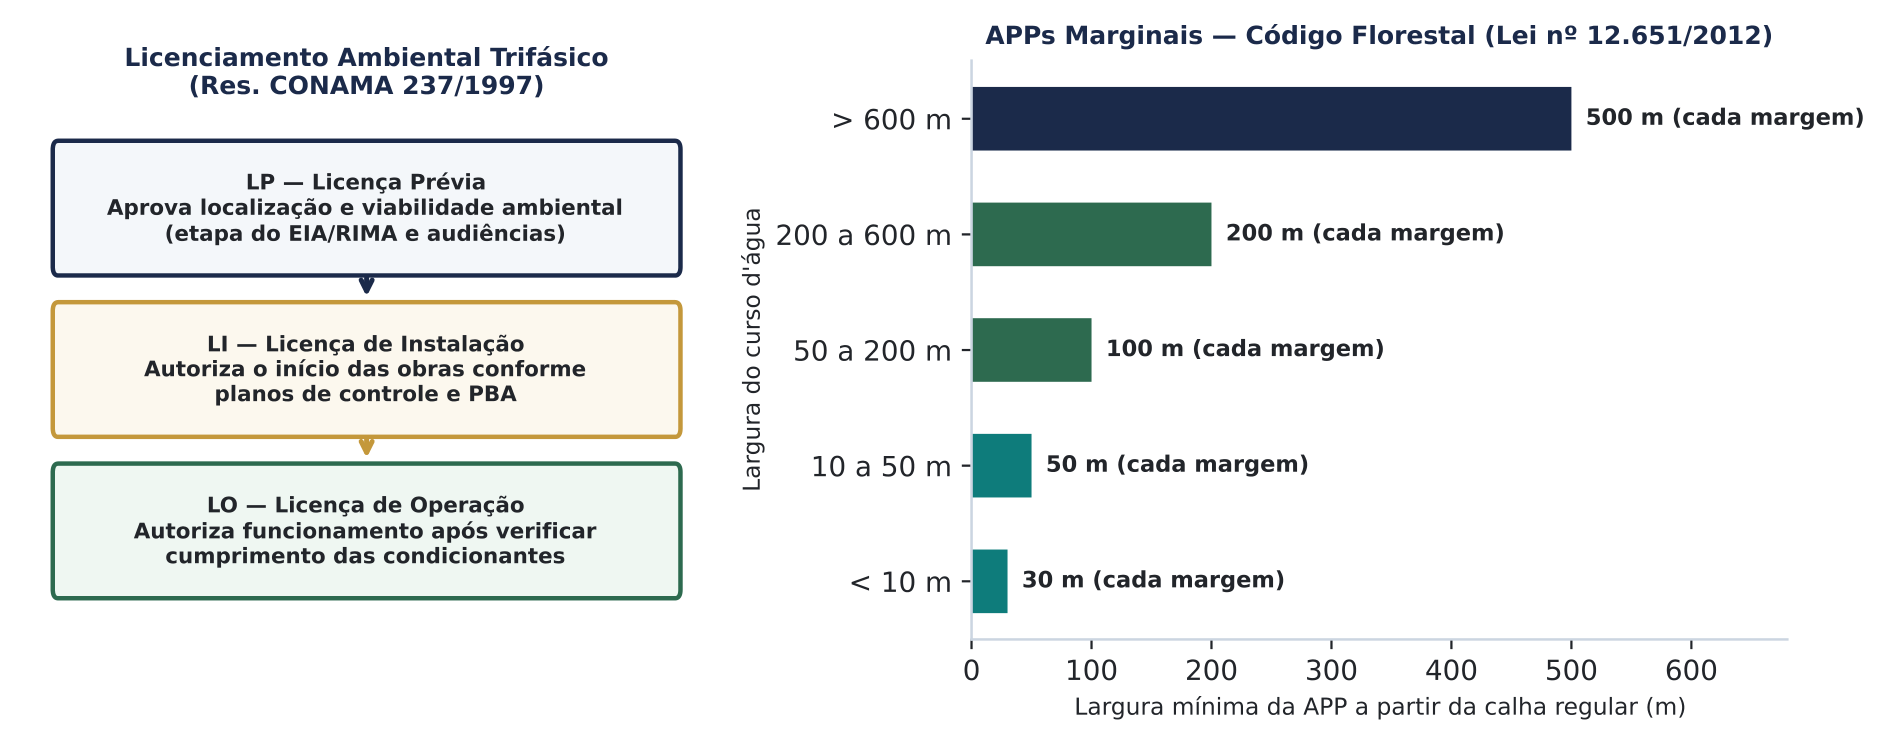
\includegraphics[keepaspectratio]{capitulos/../img/fig14_licenciamento_apps.png}}

}

\caption{\label{fig-licenciamento_apps}Integração esquemática entre o
rito do Licenciamento Ambiental Trifásico (LP, LI, LO) e a
espacialização legal das Áreas de Preservação Permanente (faixas
marginais de cursos d'água, nascentes de \(50\text{ m}\), encostas
\(> 45^\circ\) e topos de morro) e Reserva Legal em imóvel rural.}

\end{figure}%

\subsubsection{Reserva Legal (Art. 12), CAR e
PRA}\label{reserva-legal-art.-12-car-e-pra}

A \textbf{Reserva Legal (RL)} corresponde à área localizada no interior
de uma propriedade ou posse rural que deve ser mantida com cobertura de
vegetação nativa, permitindo o manejo sustentável mediante plano
aprovado, nos seguintes percentuais mínimos da área total do imóvel,

\textbf{\(80\%\)} no imóvel situado em área de \textbf{florestas} na
Amazônia Legal;. \textbf{\(35\%\)} no imóvel situado em área de
\textbf{cerrado} na Amazônia Legal;. \textbf{\(20\%\)} no imóvel situado
em área de \textbf{campos gerais} na Amazônia Legal e em \textbf{todos
os demais biomas e regiões do país} (incluindo Caatinga, Mata Atlântica
e Cerrado na Bahia).

O Art. 15 do Código Florestal admite o cômputo das APPs no cálculo do
percentual da Reserva Legal apenas quando o benefício previsto não
implicar a conversão de novas áreas para uso alternativo do solo, a área
a ser computada estiver conservada ou em processo de recuperação e o
proprietário houver efetuado a inscrição no \textbf{Cadastro Ambiental
Rural (CAR)}. O CAR é o registro público eletrônico nacional obrigatório
que reúne o perímetro georreferenciado do imóvel, suas APPs, RL,
remanescentes de vegetação nativa e áreas consolidadas, servindo como
porta de entrada para o \textbf{Programa de Regularização Ambiental
(PRA)}, mediante assinatura de Termo de Compromisso para recomposição ou
compensação de passivos.

\subsection{Cálculo Espacial de APPs e Reserva Legal em Imóvel
Rural}\label{cuxe1lculo-espacial-de-apps-e-reserva-legal-em-imuxf3vel-rural}

Para auditar um imóvel rural no CAR ou dimensionar áreas em um PRAD,
aplicam-se relações geométricas diretas,

\textbf{APP marginal de curso d'água (\(A_{\text{marg}}\)),}

\[
A_{\text{marg}} = \frac{n_m \cdot L \cdot w}{10.000} \quad (\text{em hectares})
\]

onde \(n_m \in \{1, 2\}\) indica se o curso d'água margeia o imóvel em
apenas uma margem (\(n_m = 1\)) ou atravessa o imóvel com ambas as
margens dentro da propriedade (\(n_m = 2\)), \(L\) é a extensão
longitudinal do rio no imóvel (\(\text{m}\)) e \(w\) é a largura da
faixa de APP correspondente à largura do rio (\(\text{m}\)). \textbf{APP
circular de nascente (\(A_{\text{nasc}}\)),}

\[
A_{\text{nasc}} = \frac{\pi \cdot r^2}{10.000} \quad (\text{com } r = 50\text{ m} \Rightarrow A_{\text{nasc}} \approx 0{,}7854\text{ ha por nascente isolada})
\]

. \textbf{Reserva Legal mínima exigida (\(A_{\text{RL}}\)),}

\[
A_{\text{RL}} = f_{\text{bioma}} \cdot A_{\text{imóvel}}
\]

sendo \(f_{\text{bioma}} \in \{0{,}80;\, 0{,}35;\, 0{,}20\}\) conforme a
localização do imóvel.

\subsection{PRAD e Tríplice Responsabilidade
Ambiental}\label{prad-e-truxedplice-responsabilidade-ambiental}

O \textbf{Plano de Recuperação de Áreas Degradadas (PRAD)} é o
instrumento técnico-executivo exigido tanto em processos de
licenciamento e regularização (PRA) quanto em condenações
administrativas ou judiciais para recompor funções ecológicas,
hidrológicas e edáficas de áreas alteradas. Embora modelos simplificados
variem entre órgãos (IBAMA, INEMA), a estrutura técnica completa de um
PRAD compreende cinco blocos essenciais,

\textbf{Identificação e caracterização da área.} Delimitação
cartográfica georreferenciada, histórico da degradação, diagnóstico de
solo, relevo, drenagem e cobertura vegetal remanescente.
\textbf{Isolamento dos fatores de degradação.} Cercamento contra gado,
controle de incêndios, fechamento de acessos clandestinos e eliminação
de fontes de poluição. \textbf{Preparo físico e controle erosivo
(Bioengenharia).} Reconformação de taludes, drenagem superficial,
instalação de paliçadas, biomantas e correção física/química do
substrato. \textbf{Recomposição vegetal.} Definição do método (condução
da regeneração natural, semeadura direta ou plantio de mudas em área
total/enriquecimento), escolha de espécies nativas regionais em grupos
sucessionais (pioneiras/recobrimento e secundárias tardias/diversidade),
cálculo do número de mudas e reserva de replantio.

\textbf{Cronograma e monitoramento.} Acompanhamento periódico (\(24\) a
\(60\) meses) por meio de indicadores objetivos (taxa de sobrevivência
de mudas, cobertura de copa, estabilização de sulcos e qualidade do
solo).

O descumprimento das normas ambientais submete o infrator (pessoa física
ou jurídica) à \textbf{Tríplice Responsabilidade Ambiental} consagrada
no Art. 225, §3\textsuperscript{o} da Constituição Federal e
regulamentada pela \textbf{Lei de Crimes Ambientais (Lei
n\textsuperscript{o} 9.605/1998)} e pelo Decreto n\textsuperscript{o}
6.514/2008,

\textbf{Responsabilidade Civil (Objetiva e \emph{Propter Rem}),}
obrigação de reparar integralmente o dano ambiental ou indenizá-lo,
independentemente da comprovação de culpa ou dolo (basta o nexo causal
entre a atividade e o dano). A obrigação de recompor APP e RL acompanha
o imóvel (\emph{propter rem}), transferindo-se ao sucessor em caso de
venda. \textbf{Responsabilidade Administrativa.} Aplicação de sanções
pelo poder de polícia ambiental (IBAMA, INEMA, municípios), incluindo
advertência, multa simples ou diária, apreensão de equipamentos, embargo
de obra/atividade e suspensão de licenças.

\textbf{Responsabilidade Penal.} Aplicação de penas privativas de
liberdade, restritivas de direitos ou multa criminal a pessoas físicas e
jurídicas por condutas tipificadas como crimes ambientais (desmatar APP
sem autorização, poluir mananciais, operar empreendimento potencialmente
poluidor sem licença válida).

\subsection{Atualização normativa e coerência do
PRAD}\label{atualizauxe7uxe3o-normativa-e-coeruxeancia-do-prad}

A Lei nº 15.190/2025 passou a integrar o marco nacional do licenciamento
ambiental. O estudo do procedimento deve consultar seu
\href{https://www2.camara.leg.br/legin/fed/lei/2025/lei-15190-8-agosto-2025-797833-normaatualizada-pl.html}{texto
atualizado na Câmara dos Deputados} e relacioná-lo às competências
previstas na Lei Complementar nº 140/2011. A sequência LP, LI e LO
permanece uma referência de estudo, enquanto o enquadramento depende das
modalidades e condições aplicáveis ao caso.

A caracterização de APP deve diferenciar a regra geral de proteção e as
disposições específicas aplicáveis à situação analisada. Curso de água,
nascente, reservatório e área rural consolidada possuem critérios
próprios. O relatório precisa informar a feição reconhecida e o
dispositivo utilizado para delimitar sua proteção.

O PRAD deve partir do processo responsável pela degradação. A
revegetação de uma superfície cuja drenagem continua concentrando
enxurradas pode apresentar baixa persistência. A proposta precisa
relacionar controle da causa, preparação do terreno, estabelecimento
vegetal e manutenção ao funcionamento da área.

Metas de execução registram o que foi implantado, enquanto metas
ambientais verificam a resposta do local. O documento deve indicar
período de avaliação, referência de comparação e critério de revisão.
Essa ligação entre diagnóstico e acompanhamento permite avaliar o
resultado da recuperação e ajustar as medidas quando as condições
observadas exigirem mudança.

\section{Etapa 4 - Exemplos
resolvidos}\label{etapa-4---exemplos-resolvidos-13}

\subsection{Exemplo 1. Delimitação de APPs e Reserva Legal em Imóvel
Rural na
Bahia}\label{exemplo-1.-delimitauxe7uxe3o-de-apps-e-reserva-legal-em-imuxf3vel-rural-na-bahia}

\textbf{Situação analisada.} Durante a análise ambiental de uma
propriedade rural localizada no interior da Bahia (bioma Caatinga, fora
da Amazônia Legal), necessita-se quantificar a área total de APP e a
área mínima de Reserva Legal para conferência do CAR.

\textbf{Dados disponíveis.} Área total do imóvel
\(A_{\text{imóvel}} = 250{,}0\text{ ha}\); o imóvel é margeado em apenas
um dos lados (\(n_m = 1\)) por um rio perene de \(35\text{ m}\) de
largura ao longo de \(1.200\text{ m}\) de extensão; no interior da
propriedade existe ainda \(1\) nascente perene isolada (sem sobreposição
espacial com a faixa do rio).

\textbf{Problema a resolver.} Calcule a área da APP marginal
(\(A_{\text{marg}}\)), a área da APP de nascente (\(A_{\text{nasc}}\)),
a área total de APP do imóvel e a área mínima exigida de Reserva Legal
(\(A_{\text{RL}}\)).

\textbf{Fundamento da análise.} Aplicação dos parâmetros do Art.
4\textsuperscript{o} e Art. 12 da Lei n\textsuperscript{o} 12.651/2012 e
conversão de \(\text{m}^2\) para hectares
(\(1\text{ ha} = 10.000\text{ m}^2\)).

\textbf{Desenvolvimento.} 1. Largura de APP para rio de \(35\text{ m}\)
(faixa entre \(10\text{ m}\) e \(50\text{ m}\)), \(w = 50\text{ m}\). 2.
Área da APP marginal (\(n_m = 1\)),

\[
A_{\text{marg}} = \frac{1 \times 1.200 \times 50}{10.000} = \frac{60.000}{10.000} = 6{,}00\text{ ha}
\]

\begin{enumerate}
\def\labelenumi{\arabic{enumi}.}
\setcounter{enumi}{2}
\tightlist
\item
  Área da APP da nascente perene (\(r = 50\text{ m}\)),
\end{enumerate}

\[
A_{\text{nasc}} = \frac{\pi \cdot 50^2}{10.000} = \frac{3{,}1416 \times 2.500}{10.000} \approx 0{,}79\text{ ha}
\]

\begin{enumerate}
\def\labelenumi{\arabic{enumi}.}
\setcounter{enumi}{3}
\tightlist
\item
  Área total de APP no imóvel (sem sobreposição),
\end{enumerate}

\[
A_{\text{APP}} = 6{,}00 + 0{,}79 = 6{,}79\text{ ha}
\]

\begin{enumerate}
\def\labelenumi{\arabic{enumi}.}
\setcounter{enumi}{4}
\tightlist
\item
  Reserva Legal mínima exigida na Bahia
  (\(f_{\text{bioma}} = 20\% = 0{,}20\)),
\end{enumerate}

\[
A_{\text{RL}} = 0{,}20 \times 250{,}0 = 50{,}00\text{ ha}
\]

\textbf{Interpretação do resultado.}
\(A_{\text{marg}} = 6{,}00\text{ ha}\);
\(A_{\text{nasc}} = 0{,}79\text{ ha}\);
\(A_{\text{APP}} = 6{,}79\text{ ha}\); Reserva Legal mínima
\(A_{\text{RL}} = 50{,}00\text{ ha}\).

\textbf{Condições de validade.} O rio de \(35\text{ m}\) enquadra-se
corretamente na faixa de \(10\text{ m}\) a \(50\text{ m}\) (APP de
\(50\text{ m}\)), e a Bahia situa-se integralmente fora da Amazônia
Legal, aplicando-se o percentual de \(20\%\) de Reserva Legal.

\subsection{Exemplo 2. Verificação do Cômputo de APP na Reserva Legal
(Art. 15 do Código
Florestal)}\label{exemplo-2.-verificauxe7uxe3o-do-cuxf4mputo-de-app-na-reserva-legal-art.-15-do-cuxf3digo-florestal}

\textbf{Situação analisada.} Um imóvel rural de \(400{,}0\text{ ha}\)
situado em área de cerrado dentro da Amazônia Legal (percentual legal de
Reserva Legal de \(35\%\)) busca regularização ambiental no CAR/PRA sem
realizar novas supressões.

\textbf{Dados disponíveis.} Área total \(= 400{,}0\text{ ha}\);
percentual de RL exigido \(= 35\%\); área de APP integralmente
conservada \(= 60{,}0\text{ ha}\); área de vegetação nativa conservada
fora da APP \(= 90{,}0\text{ ha}\). O proprietário não converteu novas
áreas e inscreveu o imóvel no CAR.

\textbf{Problema a resolver.} Calcule a área de RL exigida, verifique o
déficit existente sem cômputo da APP e avalie se o cômputo previsto no
Art. 15 da Lei n\textsuperscript{o} 12.651/2012 regulariza o imóvel.

\textbf{Fundamento da análise.} Cálculo da RL exigida
(\(0{,}35 \cdot A_{\text{imóvel}}\)) e soma condicionada da APP
conservada à vegetação nativa remanescente.

\textbf{Desenvolvimento.} 1. Reserva Legal mínima exigida (\(35\%\)),

\[
A_{\text{RL, exigida}} = 0{,}35 \times 400{,}0 = 140{,}0\text{ ha}
\]

\begin{enumerate}
\def\labelenumi{\arabic{enumi}.}
\setcounter{enumi}{1}
\tightlist
\item
  Balanço sem cômputo da APP,
\end{enumerate}

\[
\text{Déficit} = 140{,}0 - 90{,}0 = 50{,}0\text{ ha}
\]

\begin{enumerate}
\def\labelenumi{\arabic{enumi}.}
\setcounter{enumi}{2}
\tightlist
\item
  Balanço com cômputo da APP (atendidos os requisitos do Art. 15),
\end{enumerate}

\[
A_{\text{RL, computada}} = 90{,}0 + 60{,}0 = 150{,}0\text{ ha} \quad \left(\frac{150{,}0}{400{,}0} = 37{,}5\% > 35\%\right)
\]

\begin{enumerate}
\def\labelenumi{\arabic{enumi}.}
\setcounter{enumi}{3}
\tightlist
\item
  Saldo excedente de vegetação nativa,
\end{enumerate}

\[
\text{Excedente} = 150{,}0 - 140{,}0 = 10{,}0\text{ ha}
\]

\textbf{Interpretação do resultado.} Sem cômputo, haveria déficit de
\(50{,}0\text{ ha}\); aplicando o Art. 15, o imóvel soma
\(150{,}0\text{ ha}\) (\(37{,}5\%\)), cumprindo integralmente os
\(140{,}0\text{ ha}\) exigidos com \(10{,}0\text{ ha}\) excedentes.

\textbf{Condições de validade.} O cômputo da APP não transforma a APP em
área explorável para corte raso; ela continua sob proteção integral do
Art. 4\textsuperscript{o}, apenas contribuindo para o atingimento do
percentual mínimo de RL quando cumpridas todas as exigências legais.

\subsection{Exemplo 3. Dimensionamento de Mudas e Grupos Ecológicos em
PRAD}\label{exemplo-3.-dimensionamento-de-mudas-e-grupos-ecoluxf3gicos-em-prad}

\textbf{Situação analisada.} Para cumprir um Termo de Compromisso no
PRA, elabora-se o PRAD de uma área degradada em APP de margem fluvial
que será recuperada por plantio total de espécies nativas regionais.

\textbf{Dados disponíveis.} Área a recuperar \(A = 4{,}50\text{ ha}\)
(\(45.000\text{ m}^2\)); espaçamento adotado entre mudas de
\(3{,}0\text{ m} \times 2{,}0\text{ m}\) (\(6{,}0\text{ m}^2\) por
muda); composição florística composta por \(60\%\) de espécies de
recobrimento (pioneiras e secundárias iniciais) e \(40\%\) de espécies
de diversidade (secundárias tardias e clímax); reserva técnica de
\(15\%\) sobre o plantio inicial para replantio de falhas.

\textbf{Problema a resolver.} Calcule o número base de mudas para o
plantio inicial, a quantidade destinada a cada grupo ecológico, a
reserva de replantio e o total de mudas a adquirir no viveiro.

\textbf{Fundamento da análise.} Divisão da área total pela área útil por
cova e repartição proporcional por grupo sucessional.

\textbf{Desenvolvimento.} 1. Quantidade base de mudas para o plantio
inicial,

\[
N_{\text{base}} = \frac{45.000\text{ m}^2}{6{,}0\text{ m}^2\cdot\text{muda}^{-1}} = 7.500\text{ mudas}
\]

\begin{enumerate}
\def\labelenumi{\arabic{enumi}.}
\setcounter{enumi}{1}
\tightlist
\item
  Repartição do plantio inicial por grupo ecológico,
\end{enumerate}

\[
N_{\text{recobrimento}} = 7.500 \times 0{,}60 = 4.500\text{ mudas}
\]

\[
N_{\text{diversidade}} = 7.500 \times 0{,}40 = 3.000\text{ mudas}
\]

\begin{enumerate}
\def\labelenumi{\arabic{enumi}.}
\setcounter{enumi}{2}
\tightlist
\item
  Reserva técnica de \(15\%\) para replantio,
\end{enumerate}

\[
N_{\text{replantio}} = 7.500 \times 0{,}15 = 1.125\text{ mudas}
\]

\begin{enumerate}
\def\labelenumi{\arabic{enumi}.}
\setcounter{enumi}{3}
\tightlist
\item
  Total geral de mudas a adquirir,
\end{enumerate}

\[
N_{\text{total}} = 7.500 + 1.125 = 8.625\text{ mudas}
\]

\textbf{Interpretação do resultado.} Plantio inicial de \(7.500\) mudas
(\(4.500\) de recobrimento e \(3.000\) de diversidade), acrescido de
\(1.125\) mudas para replantio, totalizando \(8.625\) mudas.

\textbf{Condições de validade.} A densidade de
\(1.667\text{ mudas}\cdot\text{ha}^{-1}\) (\(7.500 / 4{,}5\))
corresponde exatamente ao padrão clássico de
\(3{,}0\text{ m} \times 2{,}0\text{ m}\) adotado em projetos de
restauração florestal.

\subsection{Exemplo 4. Análise de Responsabilidade Administrativa e
Civil por Supressão em
APP}\label{exemplo-4.-anuxe1lise-de-responsabilidade-administrativa-e-civil-por-supressuxe3o-em-app}

\textbf{Situação analisada.} Durante vistoria fiscalizatória em uma
propriedade rural, constatou-se o desmatamento não autorizado de
vegetação nativa em APP marginal para implantação de pastagem.

\textbf{Dados disponíveis.} Área suprimida irregularmente
\(= 3{,}60\text{ ha}\); valor-base didático de multa administrativa
adotado no exercício \(= \text{R\$ }5.000{,}00\cdot\text{ha}^{-1}\),
acrescido de \(50\%\) por incidir especificamente em APP; custo unitário
estimado de execução e monitoramento de PRAD por \(3\) anos
\(= \text{R\$ }18.000{,}00\cdot\text{ha}^{-1}\).

\textbf{Problema a resolver.} Calcule o valor da multa administrativa, o
custo da reparação civil via PRAD e o desembolso financeiro total
estimado, explicando a relação com a esfera penal.

\textbf{Fundamento da análise.} Aplicação independente das esferas
administrativa e civil segundo o princípio da Tríplice Responsabilidade
Ambiental (Art. 225, §3\textsuperscript{o} da CF/88 e Lei
n\textsuperscript{o} 9.605/1998).

\textbf{Desenvolvimento.} 1. Multa administrativa com acréscimo de
\(50\%\) (\(1{,}50\)),

\[
M_{\text{adm}} = 3{,}60 \times 5.000{,}00 \times 1{,}50 = 18.000{,}00 \times 1{,}50 = \text{R\$ }27.000{,}00
\]

\begin{enumerate}
\def\labelenumi{\arabic{enumi}.}
\setcounter{enumi}{1}
\tightlist
\item
  Custo da obrigação civil de recomposição (PRAD),
\end{enumerate}

\[
C_{\text{PRAD}} = 3{,}60 \times 18.000{,}00 = \text{R\$ }64.800{,}00
\]

\begin{enumerate}
\def\labelenumi{\arabic{enumi}.}
\setcounter{enumi}{2}
\tightlist
\item
  Desembolso total nas esferas administrativa e civil,
\end{enumerate}

\[
C_{\text{total}} = 27.000{,}00 + 64.800{,}00 = \text{R\$ }91.800{,}00
\]

\textbf{Interpretação do resultado.} Multa administrativa de
\(\text{R\$ }27.000{,}00\) e custo de PRAD de
\(\text{R\$ }64.800{,}00\), somando \(\text{R\$ }91.800{,}00\), sem
prejuízo da eventual responsabilização penal (Art. 38 da Lei
n\textsuperscript{o} 9.605/1998).

\textbf{Condições de validade.} O pagamento da multa administrativa não
dispensa o infrator da obrigação civil de recuperar a APP, pois as três
esferas são independentes e cumulativas.

\subsection{Exemplo 5. Auditoria de Prazos e Etapas no Licenciamento
Ambiental
Trifásico}\label{exemplo-5.-auditoria-de-prazos-e-etapas-no-licenciamento-ambiental-trifuxe1sico}

\textbf{Situação analisada.} Um empreendimento energético de médio
impacto ambiental na Bahia obteve sua Licença de Operação (LO) junto ao
órgão estadual competente (INEMA) após cumprir o rito trifásico.

\textbf{Dados disponíveis.} Data de emissão da LO, \(10/08/2026\); prazo
de validade concedido na LO, \(6\) anos (vencimento em \(10/08/2032\)).

\textbf{Problema a resolver.} Indique as atividades permitidas em cada
fase anterior (LP e LI), verifique se o prazo de \(6\) anos está dentro
do intervalo legal da LO e determine a data limite para protocolar o
pedido de renovação da LO com prorrogação automática.

\textbf{Fundamento da análise.} Confronto com os limites da Resolução
CONAMA n\textsuperscript{o} 237/1997 (Art. 18) e da Lei Complementar
n\textsuperscript{o} 140/2011 (Art. 14, §4\textsuperscript{o}).

\textbf{Desenvolvimento.} 1. Verificação do prazo de validade da LO, a
legislação fixa o intervalo de \(4\) a \(10\) anos para LO. Portanto,
\(6\) anos está integralmente dentro da faixa legal. 2. Antecedência
mínima legal para protocolo de renovação, \(120\) dias antes do
vencimento (\(10/08/2032\)). 3. Contagem regressiva de \(120\) dias
antes de \(10/08/2032\),

Agosto, \(10\) dias (\(01\) a \(10/08\)); restam \(110\) dias. Julho,
\(31\) dias; restam \(79\) dias. Junho, \(30\) dias; restam \(49\) dias.
Maio, \(31\) dias; restam \(18\) dias. Abril (30 dias),
\(30 - 18 = 12 \rightarrow\) data limite em \textbf{12/04/2032}.

\textbf{Interpretação do resultado.} A LP aprova apenas
concepção/localização e a LI autoriza a obra; o prazo de \(6\) anos da
LO é válido (\(4\) a \(10\) anos); o pedido de renovação deve ser
protocolado até \textbf{12/04/2032} para garantir a prorrogação
automática.

\textbf{Condições de validade.} Caso o empreendedor protocole após o
prazo de \(120\) dias e a licença vença sem análise, a operação torna-se
irregular, sujeitando o responsável a embargo e autuação.

\section{Etapa 5 - Erros de
interpretação}\label{etapa-5---erros-de-interpretauxe7uxe3o-13}

\subsection{Erro 1, Iniciar Obras Apenas com a Licença Prévia
(LP)}\label{erro-1-iniciar-obras-apenas-com-a-licenuxe7a-pruxe9via-lp}

A Licença Prévia atesta somente a viabilidade locacional e ambiental do
projeto. Realizar supressão vegetal, abertura de acessos ou
terraplenagem com base apenas na LP configura instalação sem licença
válida, gerando embargo imediato da obra, multa administrativa e crime
ambiental (Art. 60 da Lei n\textsuperscript{o} 9.605/1998).

\subsection{Erro 2, Medir a APP Marginal a Partir do Espelho d'Água da
Estiagem}\label{erro-2-medir-a-app-marginal-a-partir-do-espelho-duxe1gua-da-estiagem}

No Semiárido e em rios sazonais, o espelho d'água reduz-se drasticamente
na seca (ou desaparece nos rios intermitentes). O Art.
4\textsuperscript{o} do Código Florestal determina que a faixa de APP
seja medida a partir da \textbf{borda da calha do leito regular}, e não
do filete d'água momentâneo da estação seca.

\subsection{Erro 3, Confundir Recuperação de APP com Compensação em
Outro
Imóvel}\label{erro-3-confundir-recuperauxe7uxe3o-de-app-com-compensauxe7uxe3o-em-outro-imuxf3vel}

Enquanto o passivo de Reserva Legal pode ser compensado fora do imóvel
(via Cota de Reserva Ambiental ou área equivalente no mesmo bioma),
passivos em \textbf{Áreas de Preservação Permanente} exigem recomposição
física \emph{in loco} na própria área protegida, pois sua função
hidrogeomorfológica é intransferível.

\subsection{Erro 4, Tratar a Tríplice Responsabilidade como Alternativa
(``Paga Multa ou
Recupera'')}\label{erro-4-tratar-a-truxedplice-responsabilidade-como-alternativa-paga-multa-ou-recupera}

Um equívoco frequente é supor que o pagamento de multa administrativa
encerra o problema ambiental. Na realidade, as esferas civil,
administrativa e penal são independentes, o infrator paga a multa
(administrativa), continua obrigado a recuperar integralmente a área via
PRAD (civil) e pode responder a processo criminal (penal).

\section{Etapa 6 - Exercícios de
fixação}\label{etapa-6---exercuxedcios-de-fixauxe7uxe3o-13}

\subsubsection{Bloco A, Questões Conceituais Básicas (1 a
5)}\label{bloco-a-questuxf5es-conceituais-buxe1sicas-1-a-5-1}

\begin{enumerate}
\def\labelenumi{\arabic{enumi}.}
\item
  Cite os objetivos principais da Política Nacional do Meio Ambiente
  (Lei n\textsuperscript{o} 6.938/1981) e explique a função do CONAMA e
  dos órgãos executores/seccionais (IBAMA e INEMA) dentro do SISNAMA.
\item
  Diferencie o escopo técnico e jurídico da Licença Prévia (LP), da
  Licença de Instalação (LI) e da Licença de Operação (LO).
\item
  Explique a diferença entre o EIA (Estudo de Impacto Ambiental) e o
  RIMA (Relatório de Impacto Ambiental), indicando em qual etapa do
  licenciamento são analisados.
\item
  Distinga a função ambiental e o regime jurídico da Área de Preservação
  Permanente (APP) em relação à Reserva Legal (RL) no Código Florestal.
\item
  Descreva os cinco blocos técnicos mínimos que estruturam um Plano de
  Recuperação de Áreas Degradadas (PRAD).
\end{enumerate}

\subsubsection{Bloco B, Questões Intermediárias e Quantitativas (6 a
10)}\label{bloco-b-questuxf5es-intermediuxe1rias-e-quantitativas-6-a-10-1}

\begin{enumerate}
\def\labelenumi{\arabic{enumi}.}
\setcounter{enumi}{5}
\item
  Uma propriedade rural de \(180{,}0\text{ ha}\) na Bahia é atravessada
  por um riacho de \(6{,}0\text{ m}\) de largura média (ambas as margens
  no interior do imóvel, \(n_m = 2\)) ao longo de \(800\text{ m}\) de
  extensão, possuindo ainda \(2\) nascentes perenes isoladas. Calcule a
  área total de APP do imóvel e a área mínima exigida de Reserva Legal.
\item
  Um imóvel de \(500{,}0\text{ ha}\) situado em área de floresta na
  Amazônia Legal possui \(310{,}0\text{ ha}\) de vegetação nativa fora
  de APP e \(100{,}0\text{ ha}\) de APP conservada. Determine a RL
  exigida (\(80\%\)), verifique se há déficit sem o cômputo da APP e
  avalie se o cômputo do Art. 15 supre integralmente a exigência legal.
\item
  Para recuperar uma área alterada de \(3{,}00\text{ ha}\)
  (\(30.000\text{ m}^2\)) em APP, um PRAD especifica plantio de mudas
  nativas no espaçamento \(2{,}5\text{ m} \times 2{,}0\text{ m}\)
  (\(5{,}0\text{ m}^2\) por muda), com \(50\%\) de pioneiras/secundárias
  iniciais e \(50\%\) de secundárias tardias/clímax, além de \(10\%\) de
  reserva para replantio. Calcule o total de mudas a adquirir.
\item
  Uma indústria recebeu sua Licença de Instalação (LI) com validade de
  \(4\) anos e, após concluir a obra, obteve a LO em \(15/05/2027\) com
  validade de \(5\) anos. Indique a data de vencimento da LO e a data
  limite para protocolar o pedido de renovação com antecedência mínima
  de \(120\) dias.
\item
  Um empreendimento suprimiu irregularmente \(2{,}50\text{ ha}\) de
  vegetação nativa fora de APP, sofrendo multa didática de
  \(\text{R\$ }4.000{,}00\cdot\text{ha}^{-1}\) e obrigação de executar
  PRAD orçado em \(\text{R\$ }14.000{,}00\cdot\text{ha}^{-1}\). Calcule
  o custo total nas esferas administrativa e civil.
\end{enumerate}

\subsubsection{Bloco C, Questões Objetivas de Múltipla Escolha (11 a
15)}\label{bloco-c-questuxf5es-objetivas-de-muxfaltipla-escolha-11-a-15-1}

\begin{enumerate}
\def\labelenumi{\arabic{enumi}.}
\setcounter{enumi}{10}
\item
  No âmbito do SISNAMA (Lei n\textsuperscript{o} 6.938/1981), o órgão
  consultivo e deliberativo responsável por estabelecer normas e padrões
  ambientais nacionais mediante resoluções é o,

  \begin{enumerate}
  \def\labelenumii{(\Alph{enumii})}
  \item
    IBAMA.
  \item
    CONAMA.
  \item
    INEMA.
  \item
    ICMBio.
  \item
    Ministério Público Federal.
  \end{enumerate}
\item
  De acordo com a Lei n\textsuperscript{o} 12.651/2012 (Art.
  4\textsuperscript{o}), a faixa mínima de Área de Preservação
  Permanente para um curso d'água natural com \(75\text{ m}\) de largura
  de calha regular e para uma nascente perene são, respectivamente,

  \begin{enumerate}
  \def\labelenumii{(\Alph{enumii})}
  \item
    \(50\text{ m}\) e \(30\text{ m}\).
  \item
    \(100\text{ m}\) e \(50\text{ m}\).
  \item
    \(200\text{ m}\) e \(50\text{ m}\).
  \item
    \(100\text{ m}\) e \(100\text{ m}\).
  \item
    \(30\text{ m}\) e \(50\text{ m}\).
  \end{enumerate}
\item
  Os percentuais mínimos de Reserva Legal exigidos pelo Código Florestal
  para imóveis situados na Amazônia Legal em áreas de floresta, cerrado
  e campos gerais são, respectivamente,

  \begin{enumerate}
  \def\labelenumii{(\Alph{enumii})}
  \item
    \(80\%\), \(35\%\) e \(20\%\).
  \item
    \(80\%\), \(50\%\) e \(20\%\).
  \item
    \(50\%\), \(35\%\) e \(20\%\).
  \item
    \(80\%\), \(20\%\) e \(20\%\).
  \item
    \(35\%\), \(20\%\) e \(20\%\).
  \end{enumerate}
\item
  Sobre a Tríplice Responsabilidade Ambiental no ordenamento jurídico
  brasileiro, é correto afirmar que,

  \begin{enumerate}
  \def\labelenumii{(\Alph{enumii})}
  \item
    A responsabilidade civil ambiental é subjetiva, exigindo sempre a
    prova de intenção dolosa do degradador.
  \item
    O pagamento da multa administrativa extingue automaticamente a
    obrigação de reparar o dano em PRAD.
  \item
    As sanções administrativas, civis e penais podem incidir
    cumulativamente sobre o mesmo fato danoso, sendo objetiva a
    obrigação civil de reparar o dano.
  \item
    Pessoas jurídicas não podem ser responsabilizadas na esfera penal
    por crimes ambientais no Brasil.
  \item
    A obrigação de recompor a Reserva Legal desaparece quando o imóvel
    rural é vendido a terceiros.
  \end{enumerate}
\item
  No Licenciamento Ambiental Trifásico (Resolução CONAMA
  n\textsuperscript{o} 237/1997), a licença que autoriza o início
  efetivo das obras civis e da instalação dos equipamentos, mediante
  atendimento às condicionantes da fase preliminar, é a,

  \begin{enumerate}
  \def\labelenumii{(\Alph{enumii})}
  \item
    Licença Prévia (LP).
  \item
    Licença de Instalação (LI).
  \item
    Licença de Operação (LO).
  \item
    Outorga Preventiva de Uso da Água.
  \item
    Certidão de Cadastro Ambiental Rural (CAR).
  \end{enumerate}
\end{enumerate}

\section{Etapa 7 - Questões de
aplicação}\label{etapa-7---questuxf5es-de-aplicauxe7uxe3o-13}

\subsection{Foco de Provas, ENADE e Concursos (IBAMA / INEMA /
Perícia)}\label{foco-de-provas-enade-e-concursos-ibama-inema-peruxedcia}

Questões de concursos e do ENADE frequentemente apresentam situações
reais de campo em que um proprietário ou empreendedor confunde fases do
licenciamento, mede APPs de forma equivocada ou tenta compensar APP fora
do imóvel. Domine os números exatos da Lei n\textsuperscript{o}
12.651/2012 e a independência das três esferas de responsabilidade.

\begin{enumerate}
\def\labelenumi{\arabic{enumi}.}
\setcounter{enumi}{15}
\item
  \textbf{{[}Questão Autoral, Estilo ENADE / Geografia{]}} Durante
  visita técnica a uma propriedade rural localizada no Semiárido Baiano,
  estudantes da disciplina Análise Ambiental observaram que um trecho de
  \(600\text{ m}\) da margem de um rio perene de \(15\text{ m}\) de
  largura encontrava-se desmatado e com sulcos erosivos ativos. O
  proprietário afirmou que não havia necessidade de recomposição porque,
  (1) a faixa desmatada media \(30\text{ m}\) de largura a partir do
  espelho d'água atual na estação seca; e (2) ele pretendia comprar uma
  área de Caatinga preservada em outro município para ``compensar a
  APP'' desmatada. À luz da Lei n\textsuperscript{o} 12.651/2012, avalie
  as afirmações,

  \begin{itemize}
  \item
    Para um curso d'água de \(15\text{ m}\) de largura, a APP marginal
    mínima é de \(50\text{ m}\) medidos a partir da borda da calha do
    leito regular, e não do espelho d'água da estiagem.
  \item
    A compensação em outro imóvel rural aplica-se a déficits de Reserva
    Legal, não substituindo a obrigação de recompor fisicamente a APP
    degradada no próprio imóvel.
  \item
    Por se tratar de propriedade situada na Bahia, o percentual mínimo
    de Reserva Legal exigido é de \(35\%\).
  \end{itemize}

  É correto o que se afirma em,

  \begin{enumerate}
  \def\labelenumii{(\Alph{enumii})}
  \item
    I, apenas.
  \item
    III, apenas.
  \item
    I e II, apenas.
  \item
    II e III, apenas.
  \item
    I, II e III.
  \end{enumerate}
\item
  \textbf{{[}Questão Autoral, Estilo Concurso Analista Ambiental /
  INEMA-BA{]}} Um empreendimento com potencial de significativa
  degradação ambiental protocolou pedido de licenciamento junto ao órgão
  estadual competente. Considerando a Resolução CONAMA
  n\textsuperscript{o} 001/1986 e a Resolução CONAMA
  n\textsuperscript{o} 237/1997, assinale a sequência correta de
  procedimentos administrativos,

  \begin{enumerate}
  \def\labelenumii{(\Alph{enumii})}
  \item
    Emissão da LI para abertura do canteiro de obras \(\rightarrow\)
    elaboração do EIA/RIMA durante a operação \(\rightarrow\) emissão da
    LP ao final da vida útil.
  \item
    Elaboração do EIA/RIMA e realização de audiência pública
    \(\rightarrow\) análise e emissão da LP (viabilidade locacional)
    \(\rightarrow\) aprovação dos projetos executivos e emissão da LI
    (autorização de obras) \(\rightarrow\) verificação das
    condicionantes e emissão da LO (funcionamento).
  \item
    Inscrição no CAR \(\rightarrow\) dispensa de LP e LI \(\rightarrow\)
    emissão direta da LO por autodeclaração.
  \item
    Emissão simultânea de LP, LI e LO sem vistoria prévia para qualquer
    obra energética de grande porte.
  \item
    Elaboração apenas do RIMA simplificado sem EIA técnico, sendo
    facultativa a apresentação de alternativas locacionais.
  \end{enumerate}
\item
  \textbf{{[}Questão Autoral, Estilo Concurso Analista Ambiental /
  IBAMA{]}} Em razão de vazamento de efluentes industriais não
  licenciados que provocou mortandade de peixes e contaminação de margem
  fluvial, o órgão ambiental lavrou auto de infração com multa, o
  Ministério Público ajuizou ação civil pública exigindo PRAD e
  indenização, e foi instaurado processo criminal com base na Lei
  n\textsuperscript{o} 9.605/1998. A defesa da empresa alegou que não
  houve intenção de poluir e que o pagamento da multa administrativa já
  impediria outras cobranças. Sob o ponto de vista jurídico-ambiental
  brasileiro, a tese da defesa é,

  \begin{enumerate}
  \def\labelenumii{(\Alph{enumii})}
  \item
    Procedente, pois a responsabilidade civil ambiental exige
    comprovação de dolo específico.
  \item
    Procedente, pois o princípio da unicidade impede a cumulação de
    multa administrativa com ação penal.
  \item
    Improcedente, pois a responsabilidade civil ambiental é objetiva
    (independe de culpa ou dolo) e as esferas civil, administrativa e
    penal são independentes e cumulativas.
  \item
    Parcialmente procedente, pois empresas privadas não podem sofrer
    sanções administrativas, apenas pessoas físicas.
  \item
    Improcedente apenas quanto à multa, mas procedente quanto ao PRAD,
    que é sempre facultativo em áreas industriais.
  \end{enumerate}
\end{enumerate}

\section{Etapa 8 - Gabarito
comentado}\label{etapa-8---gabarito-comentado-13}

\subsection{Resoluções Completas, Exercícios de Fixação (1 a
15)}\label{resoluuxe7uxf5es-completas-exercuxedcios-de-fixauxe7uxe3o-1-a-15-4}

\begin{enumerate}
\def\labelenumi{\arabic{enumi}.}
\item
  A PNMA visa preservar, melhorar e recuperar a qualidade ambiental
  propícia à vida e ao desenvolvimento sustentável. No SISNAMA, o
  \textbf{CONAMA} atua como órgão consultivo e deliberativo (editando
  normas e resoluções), enquanto \textbf{IBAMA} (federal) e
  \textbf{INEMA} (estadual na Bahia) executam o licenciamento, a
  fiscalização e o controle ambiental em suas respectivas esferas de
  competência.
\item
  \textbf{LP.} Atesta viabilidade ambiental e aprova
  localização/concepção (não autoriza obra). \textbf{LI.} Autoriza a
  instalação/construção do empreendimento segundo projetos executivos
  aprovados. \textbf{LO.} Autoriza o início da operação após verificação
  do cumprimento das condicionantes anteriores.
\item
  O \textbf{EIA} é o estudo técnico-científico multidisciplinar completo
  (diagnóstico, prognóstico, impactos, alternativas e programas); o
  \textbf{RIMA} é sua síntese acessível ao público e aos conselhos.
  Ambos integram a fase preliminar de avaliação que subsidia a decisão
  sobre a \textbf{LP}.
\item
  A \textbf{APP} tem função ambiental rígida vinculada a feições
  sensíveis (rios, nascentes, encostas, topos de morro), exigindo
  preservação integral e recuperação \emph{in loco} quando degradada. A
  \textbf{Reserva Legal} é um percentual da área do imóvel rural
  (\(20\%\), \(35\%\) ou \(80\%\)) destinado à conservação da vegetação
  nativa com possibilidade de manejo sustentável e compensação legal em
  caso de passivo consolidado.
\item
  Os cinco blocos são, (1) identificação e diagnóstico da área; (2)
  isolamento dos fatores de degradação; (3) preparo físico e obras de
  controle erosivo/bioengenharia; (4) recomposição vegetal
  estratificada; (5) cronograma executivo e monitoramento por
  indicadores.
\item
  \textbf{Desenvolvimento,} Riacho de \(6{,}0\text{ m}\)
  (\(< 10\text{ m}\)), APP de \(w = 30\text{ m}\) em cada margem
  (\(n_m = 2\)). APP marginal,
  \(A_{\text{marg}} = (2 \times 800 \times 30) / 10.000 = 48.000 / 10.000 = 4{,}80\text{ ha}\).
  APP das \(2\) nascentes (\(r = 50\text{ m}\)),
  \(A_{\text{nasc}} = 2 \times (\pi \cdot 50^2 / 10.000) \approx 2 \times 0{,}7854 = 1{,}57\text{ ha}\).
  APP total, \(4{,}80 + 1{,}57 = \mathbf{6{,}37\text{ ha}}\). Reserva
  Legal mínima na Bahia (\(20\%\)),
  \(A_{\text{RL}} = 0{,}20 \times 180{,}0 = \mathbf{36{,}00\text{ ha}}\).
\item
  \textbf{Desenvolvimento,} RL exigida (\(80\%\) em floresta na Amazônia
  Legal), \(0{,}80 \times 500{,}0 = \mathbf{400{,}0\text{ ha}}\). Sem
  cômputo da APP, déficit de
  \(400{,}0 - 310{,}0 = \mathbf{90{,}0\text{ ha}}\). Com cômputo da APP
  (Art. 15), \(310{,}0 + 100{,}0 = \mathbf{410{,}0\text{ ha}}\)
  (\(82{,}0\% > 80\%\)), suprindo integralmente a exigência com
  \(10{,}0\text{ ha}\) excedentes.
\item
  \textbf{Desenvolvimento,} Mudas base, \(30.000 / 5{,}0 = 6.000\) mudas
  (\(3.000\) pioneiras/secundárias iniciais e \(3.000\) secundárias
  tardias/clímax). Reserva de replantio (\(10\%\)),
  \(6.000 \times 0{,}10 = 600\) mudas. Total a adquirir,
  \(6.000 + 600 = \mathbf{6.600\text{ mudas}}\).
\item
  \textbf{Desenvolvimento,} Vencimento da LO, \textbf{15/05/2032} (\(5\)
  anos após \(15/05/2027\)). Contagem regressiva de \(120\) dias
  (lembrando que 2032 é ano bissexto, mas fevereiro já ficou antes da
  contagem), Maio (\(15\) dias, \(01\) a \(15/05\), restam \(105\));
  Abril (\(30\) dias, restam \(75\)); Março (\(31\) dias, restam
  \(44\)); Fevereiro de 2032 (\(29\) dias, restam \(15\)); Janeiro
  (\(31 - 15 = 16 \rightarrow\) \textbf{16/01/2032}). (Em anos não
  bissextos seria 15/01; em 2032, bissexto, \(16/01/2032\) completa
  exatamente \(120\) dias até \(15/05/2032\).)
\item
  \textbf{Desenvolvimento,} Multa administrativa,
  \(2{,}50 \times 4.000{,}00 = \text{R\$ }10.000{,}00\). Custo do PRAD
  (esfera civil),
  \(2{,}50 \times 14.000{,}00 = \text{R\$ }35.000{,}00\). Total nas duas
  esferas,
  \(10.000{,}00 + 35.000{,}00 = \mathbf{\text{R\$ }45.000{,}00}\).
\item
  \textbf{Gabarito, (B).} O CONAMA é o órgão consultivo e deliberativo
  do SISNAMA.
\item
  \textbf{Gabarito, (B).} Cursos d'água entre \(50\text{ m}\) e
  \(200\text{ m}\) de largura exigem \(100\text{ m}\) de APP marginal;
  nascentes perenes exigem raio de \(50\text{ m}\).
\item
  \textbf{Gabarito, (A).} Art. 12 da Lei n\textsuperscript{o}
  12.651/2012, \(80\%\) (florestas), \(35\%\) (cerrado) e \(20\%\)
  (campos gerais) na Amazônia Legal.
\item
  \textbf{Gabarito, (C).} A responsabilidade civil ambiental é objetiva
  (baseada no risco integral e no nexo causal) e coexiste de forma
  independente com as sanções administrativas e penais.
\item
  \textbf{Gabarito, (B).} A Licença de Instalação (LI) é o ato
  administrativo que autoriza a execução física das obras e a instalação
  do empreendimento.
\end{enumerate}

\subsection{Resoluções Completas, Questões ENADE e Concursos (16 a
18)}\label{resoluuxe7uxf5es-completas-questuxf5es-enade-e-concursos-16-a-18-4}

\begin{enumerate}
\def\labelenumi{\arabic{enumi}.}
\setcounter{enumi}{15}
\item
  \textbf{Gabarito, (C).} As afirmações I e II estão corretas, rio de
  \(15\text{ m}\) exige \(50\text{ m}\) de APP medidos da borda da calha
  regular, e APP degradada deve ser recuperada no local, não cabendo
  compensação externa. A afirmação III é falsa porque a Bahia está fora
  da Amazônia Legal, aplicando-se \(20\%\) de Reserva Legal.
\item
  \textbf{Gabarito, (B).} Apenas (B) respeita a ordem cronológica e
  legal do licenciamento trifásico para obras sujeitas a EIA/RIMA,
  estudos e audiência pública prévios à LP, projetos executivos e
  autorização de obras na LI, e funcionamento autorizado na LO.
\item
  \textbf{Gabarito, (C).} A tese da defesa é improcedente em ambos os
  pontos, no Brasil, a obrigação civil de reparar o dano ambiental é
  objetiva (dispensa prova de dolo ou culpa) e as três esferas (civil,
  administrativa e penal) atuam de forma independente e cumulativa.
\end{enumerate}

\section{Etapa 9 - Síntese
conceitual}\label{etapa-9---suxedntese-conceitual-13}

\textbf{PNMA (Lei n\textsuperscript{o} 6.938/1981).} Institui o SISNAMA
(CONAMA, MMA, IBAMA, ICMBio, órgãos estaduais como INEMA e órgãos
municipais) e instrumentos como AIA, licenciamento, zoneamento e SINIMA.
\textbf{Licenciamento Trifásico (CONAMA 237/1997 e 001/1986),} LP
(viabilidade e localização; até \(5\) anos), LI (instalação/obras; até
\(6\) anos) e LO (operação; \(4\) a \(10\) anos, renovação com \(120\)
dias de antecedência); EIA/RIMA obrigatório para significativa
degradação. \textbf{Código Florestal (Lei n\textsuperscript{o}
12.651/2012),} APPs marginais de \(30\text{ m}\) a \(500\text{ m}\),
nascentes de \(50\text{ m}\), encostas \(> 45^\circ\), topos de morro,
restingas e manguezais; Reserva Legal de \(80\%\), \(35\%\) ou \(20\%\);
regularização via CAR e PRA.

\textbf{PRAD e Tríplice Responsabilidade.} Recomposição técnica com
isolamento, bioengenharia, plantio estratificado e monitoramento;
responsabilização civil objetiva, administrativa e penal cumulativas
(Lei n\textsuperscript{o} 9.605/1998).

\section{Etapa 10 - Verificação da
aprendizagem}\label{etapa-10---verificauxe7uxe3o-da-aprendizagem-13}

Avalie cada afirmação com \textbf{V} (Verdadeiro) ou \textbf{F} (Falso)
antes de conferir o gabarito abaixo,

\begin{enumerate}
\def\labelenumi{\arabic{enumi}.}
\item
  ( ) A Licença Prévia (LP) autoriza o empreendedor a realizar a
  supressão vegetal e a terraplenagem inicial do terreno enquanto
  conclui os projetos executivos para a LI.
\item
  ( ) Em um curso d'água natural de \(40\text{ m}\) de largura, a APP
  marginal mínima prevista no Código Florestal é de \(50\text{ m}\) em
  cada margem a partir da borda da calha do leito regular.
\item
  ( ) Na Bahia, o percentual mínimo de Reserva Legal exigido para
  imóveis rurais é de \(20\%\), podendo a APP conservada ser computada
  apenas quando atendidos os requisitos cumulativos do Art. 15 da Lei
  n\textsuperscript{o} 12.651/2012.
\item
  ( ) A obrigação civil de reparar o dano ambiental independe da
  comprovação de dolo ou culpa do agente, coexistindo com eventuais
  multas administrativas e sanções penais.
\end{enumerate}

\textbf{Gabarito do verificação da aprendizagem,} 1-\textbf{F}~(a
instalação e a supressão dependem da LI) \textbar-\textbf{V}
\textbar-\textbf{V} \textbar-\textbf{V}.

\chapter{Manual Prático do Diagnóstico Ambiental Aplicado e Produtos
Técnicos}\label{cap:diagnostico_final_pratico}

O diagnóstico ambiental aplicado reúne evidências para explicar o
funcionamento de uma área e orientar decisões. Mapas e indicadores
sustentam a análise quando suas relações são demonstradas. O produto
final deve permitir compreender o problema, localizar as intervenções e
verificar os resultados esperados.

\section{Etapa 1 - Objetivos de
aprendizagem}\label{etapa-1---objetivos-de-aprendizagem-14}

A aprendizagem envolve elaborar um diagnóstico com pergunta, recorte,
dados, interpretação e proposta coerentes. O estudante deve justificar
suas conclusões, reconhecer limitações e apresentar critérios de
acompanhamento que permitam revisar a intervenção.

\section{Etapa 2 - Conhecimentos
necessários}\label{etapa-2---conhecimentos-necessuxe1rios-14}

O trabalho articula leitura de paisagem, análise de bacia, solos,
indicadores e instrumentos de gestão. A integração exige que mapas e
tabelas utilizem unidades territoriais compatíveis e que diferenças de
data e método sejam consideradas na interpretação.

\section{Etapa 3 - Fundamentação
teórica}\label{etapa-3---fundamentauxe7uxe3o-teuxf3rica-14}

\subsection{Vocabulário Técnico e Símbolos do Capítulo
15}\label{vocabuluxe1rio-tuxe9cnico-e-suxedmbolos-do-capuxedtulo-15}

\textbf{Recorte Espacial (\(A_{\text{rec}}\)).} Unidade territorial
delimitada para o diagnóstico (preferencialmente microbacia
hidrográfica, sub-bacia, vertente completa ou trecho de APP/área
degradada). \textbf{SIRGAS 2000,} Sistema de Referência Geocêntrico para
as Américas, datum geodésico oficial do Brasil, obrigatório nos projetos
em QGIS e nos mapas finais. \(A_{\min}\), \textbf{área mínima mapeável}
no terreno correspondente a \(4\text{ mm}^2\) no mapa impresso
(\(A_{\min} = 4 \times 10^{-6} \cdot E^2\text{ m}^2\), onde \(E\) é o
denominador da escala \(1:E\)). \textbf{Matriz de Indicadores.} Tabela
analítica que cruza Pressão, Estado, Impacto e Resposta (PEIR) com
atributos de qualidade do solo (\(IQS\)) e fragilidade emergente
(\(FE\)).

\(IPI\), \textbf{Índice Composto de Priorização de Intervenção}
(adimensional entre \(0\) e \(1\)), usado para ranquear setores críticos
na alocação de bioengenharia e PRAD. \(CE\), \textbf{Custo-Efetividade}
de uma intervenção (\(\text{t}\cdot\text{ano}^{-1}\) de sedimentos
retidos por \(\text{R\$ }1.000,00\) investidos).

O Trabalho Prático Final da disciplina CHF662 representa \(50\%\) da
avaliação semestral (\(5{,}0\) pontos) e simula a entrega de um
diagnóstico técnico profissional em Análise Ambiental. Conforme ilustra
a Figura~\ref{fig-fluxo_diagnostico_final}, o fluxo metodológico
articula sete etapas encadeadas, da delimitação espacial à socialização
dos resultados.

\begin{figure}[H]

\centering{

\pandocbounded{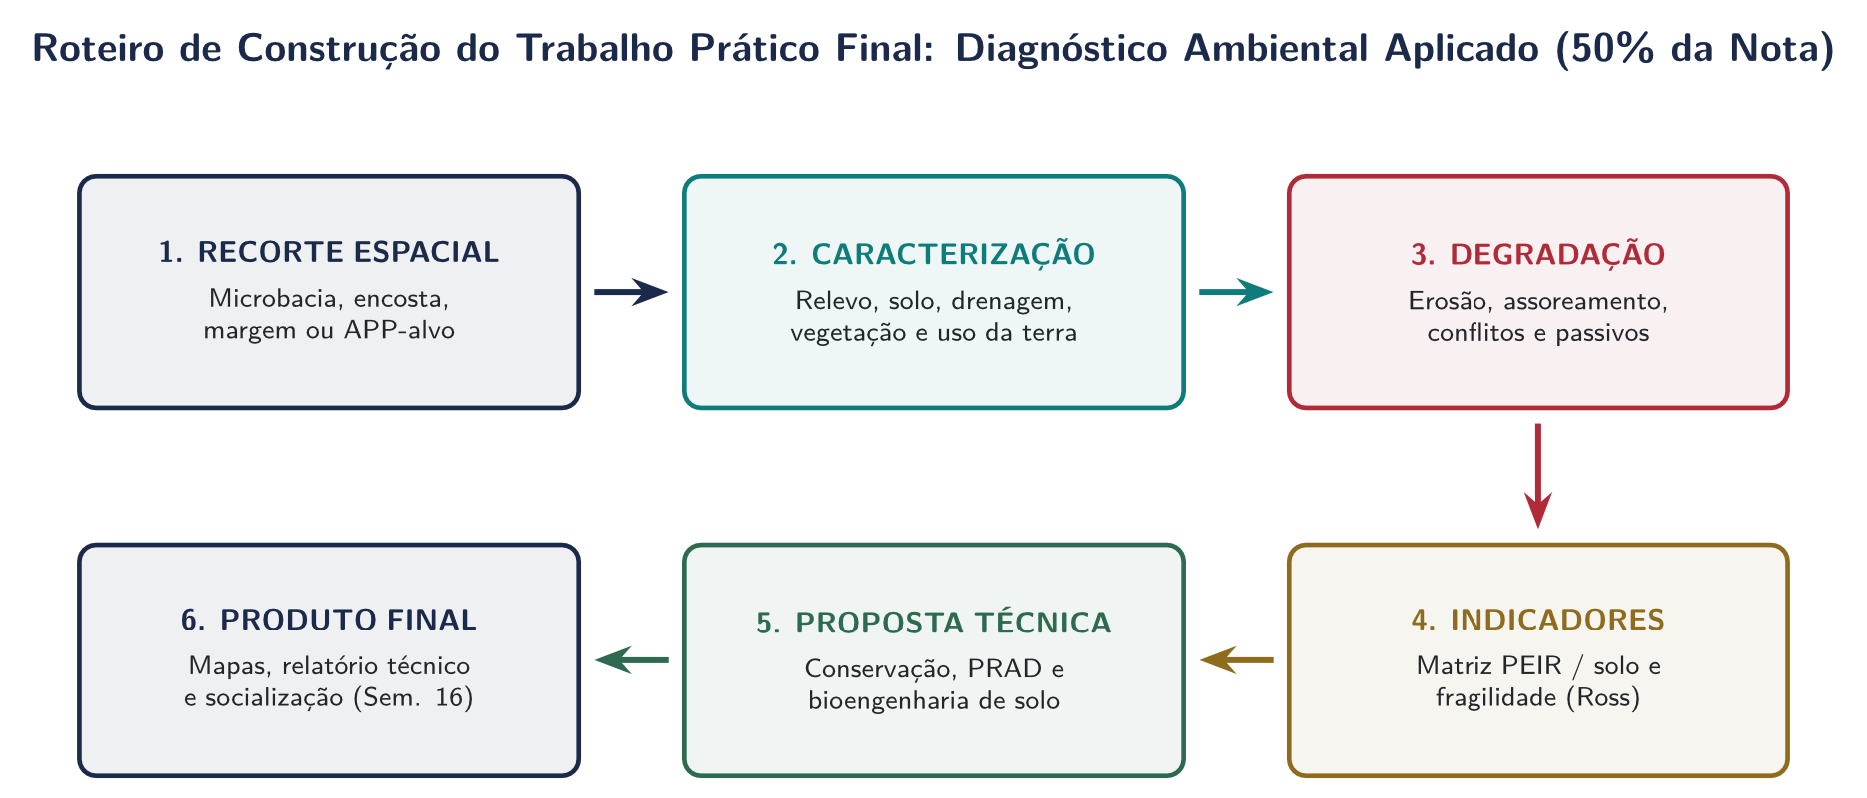
\includegraphics[keepaspectratio]{capitulos/../img/fig15_fluxo_diagnostico_final.png}}

}

\caption{\label{fig-fluxo_diagnostico_final}Fluxograma operacional das
sete etapas do Diagnóstico Ambiental Aplicado (Trabalho Prático Final da
disciplina CHF662, Semana 16), integrando bases abertas, matriz de
indicadores, produtos cartográficos e proposta de intervenção.}

\end{figure}%

\section{Etapa 1, Escolha e Delimitação do Recorte
Espacial}\label{etapa-1-escolha-e-delimitauxe7uxe3o-do-recorte-espacial}

A escolha da área de estudo deve equilibrar \textbf{relevância
socioambiental} e \textbf{viabilidade de levantamento} no prazo
semestral (IBGE, 2018; Cavalcanti, 2006). O recorte pode ser,

\textbf{Microbacia hidrográfica.} Unidade preferencial por integrar
divisores de água, rede de drenagem, conectividade hidrossedimentológica
e uso da terra (área sugerida entre \(1\text{ km}^2\) e
\(50\text{ km}^2\)). \textbf{Encosta ou vertente representativa.}
Indicada quando o foco recai sobre processos erosivos lineares (sulcos,
ravinas, voçorocas) ou movimentos de massa em áreas urbanas e rurais.
\textbf{Margem de curso d'água, APP ou área degradada pontual.} Adequada
para diagnósticos de passivo florestal (Lei nº 12.651/2012),
assoreamento de açudes, antigas cascalheiras ou acessos de
empreendimentos energéticos (como observado no campo do Semiárido).

A delimitação deve ser vetorizada em polígono fechado no QGIS (formato
GeoPackage `.gpkg` ou Shapefile `.shp`), com justificativa clara dos
critérios naturais (divisores topográficos) ou legais/administrativos
(limites de APP ou poligonal de empreendimento) adotados.

\section{Etapa 2, Levantamento de Bases Cartográficas e Dados
Abertos}\label{etapa-2-levantamento-de-bases-cartogruxe1ficas-e-dados-abertos}

Todo diagnóstico ambiental auditável depende de fontes públicas
rastreáveis, organizadas em um banco geográfico padronizado em
\textbf{SIRGAS 2000} (coordenadas geográficas para abrangência regional
ou projeção UTM, fuso 24S para a maior parte da Bahia, para cálculos de
área e comprimento),

{\def\LTcaptype{none} % do not increment counter
\begin{longtable}[]{@{}
  >{\raggedright\arraybackslash}p{(\linewidth - 4\tabcolsep) * \real{0.3333}}
  >{\raggedright\arraybackslash}p{(\linewidth - 4\tabcolsep) * \real{0.3333}}
  >{\raggedright\arraybackslash}p{(\linewidth - 4\tabcolsep) * \real{0.3333}}@{}}
\toprule\noalign{}
\begin{minipage}[b]{\linewidth}\raggedright
\textbf{Base / Plataforma}
\end{minipage} & \begin{minipage}[b]{\linewidth}\raggedright
\textbf{Dados Extraídos}
\end{minipage} & \begin{minipage}[b]{\linewidth}\raggedright
\textbf{Aplicação Direta no Trabalho Final}
\end{minipage} \\
\midrule\noalign{}
\endhead
\bottomrule\noalign{}
\endlastfoot
\textbf{IBGE} & Limites municipais, malha censitária, hidrografia e
pedologia & Contextualização territorial, caracterização socioespacial e
classes de solo. \\
\textbf{SRTM / TOPODATA (INPE)} & Modelo Digital de Elevação
(\(30\text{ m}\)), declividade e curvas de nível & Delimitação
automática da microbacia, perfil de vertente, fator \(LS\) e mapa
clinográfico (Ross). \\
\textbf{MapBiomas} & Séries anuais de uso e cobertura da terra
(\(30\text{ m}\)) & Análise multitemporal (por exemplo,
\(1985\)-\(2024\)), supressão de vegetação nativa e fator \(C\) da
USLE. \\
\textbf{SICAR / CAR} & Perímetros de imóveis rurais, APPs e Reserva
Legal declaradas & Verificação de passivo ambiental em APPs marginais e
nascentes (Lei nº 12.651/2012). \\
\textbf{INEMA / SEI-BA} & Outorgas, licenças ambientais, bacias
estaduais e dados climáticos & Identificação de empreendimentos
licenciados, conflitos hídricos e erosividade regional (\(R\)). \\
\end{longtable}
}

\section{Etapa 3, Caracterização Integrada Físico-Biótica e
Socioespacial}\label{etapa-3-caracterizauxe7uxe3o-integrada-fuxedsico-biuxf3tica-e-socioespacial}

Seguindo a abordagem sistêmica de Cavalcanti (2006) e IBGE (2018), o
texto diagnóstico não deve apresentar compartimentos isolados (clima,
solo, vegetação e sociedade em blocos desconexos), mas explicar suas
\textbf{interações causais},

\textbf{Meio físico-biótico.} Articular regime pluviométrico
(concentração sazonal das chuvas), compartimentos do relevo (topo, meia
encosta, sopé e planície), classes de solo (espessura, textura e
suscetibilidade erosiva) e fisionomia vegetal remanescente (Caatinga,
Mata Atlântica, Cerrado ou vegetação ripária). \textbf{Dinâmica
socioespacial.} Relacionar formas de uso e ocupação da terra (pecuária
extensiva, agricultura de sequeiro, expansão urbana, infraestrutura
energética ou mineração), estrutura fundiária, pressões sobre os
recursos hídricos e percepção/vulnerabilidade das comunidades locais.

\section{Etapa 4, Identificação e Mapeamento de Processos de
Degradação}\label{etapa-4-identificauxe7uxe3o-e-mapeamento-de-processos-de-degradauxe7uxe3o}

Com apoio de imagens de alta resolução (Google/Bing/CBERS-4A no QGIS) e,
quando viável, verificação de campo com registro fotográfico
georreferenciado e escala métrica, devem ser inventariados os processos
ativos,

\textbf{Erosão hídrica.} Selamento superficial, erosão laminar, sulcos
(\(<0{,}5\text{ m}\)), ravinas (\(>0{,}5\text{ m}\)) e voçorocas (com
eventual exfiltração e \emph{piping}). \textbf{Degradação física do
solo.} Compactação em trilhas, estradas não pavimentadas e áreas de
pisoteio intenso. \textbf{Degradação ripária e fluvial.} Supressão de
mata ciliar em APPs, solapamento de margens e assoreamento de córregos,
barreiros ou açudes. \textbf{Passivos de resíduos ou contaminação.}
Disposição irregular de resíduos sólidos, efluentes domésticos ou
rejeitos minerários sem contenção.

\section{Etapa 5, Montagem da Matriz de Indicadores e Índice de
Priorização}\label{etapa-5-montagem-da-matriz-de-indicadores-e-uxedndice-de-priorizauxe7uxe3o}

Para evitar diagnósticos puramente descritivos, o Trabalho Prático Final
exige uma \textbf{Matriz de Indicadores} que integre o modelo
\textbf{PEIR} (Capítulo 10), os atributos de \textbf{Qualidade do Solo}
(Capítulo 11) e a \textbf{Fragilidade Emergente de Ross} (Capítulo 9).
Quando houver múltiplos setores ou subunidades na área de estudo,
aplica-se o Índice Composto de Priorização de Intervenção (\(IPI\)) para
hierarquizar onde agir primeiro.

\subsection{\texorpdfstring{Índice Composto de Priorização de
Intervenção
(\(IPI\))}{Índice Composto de Priorização de Intervenção (IPI)}}\label{uxedndice-composto-de-priorizauxe7uxe3o-de-intervenuxe7uxe3o-ipi}

Para cada setor homogêneo avaliado na área de estudo, o Índice Composto
de Priorização de Intervenção (\(IPI \in [0,\,1]\)) combina três
dimensões normalizadas,

\[
IPI = w_F \cdot F_{\text{norm}} + w_S \cdot (1 - IQS) + w_P \cdot P_{\text{norm}}
\]

em que,

\(F_{\text{norm}} = \dfrac{FE - 1}{4}\), \textbf{Fragilidade Emergente
de Ross normalizada} (\(FE \in \{1, 2, 3, 4, 5\}\) convertida para a
escala \([0,\,1]\); logo \(FE=1 \Rightarrow 0{,}00\) e
\(FE=5 \Rightarrow 1{,}00\)). \((1 - IQS)\), \textbf{Déficit de
Qualidade do Solo}, obtido a partir do Índice de Qualidade do Solo
(\(IQS \in [0,\,1]\); quanto menor o \(IQS\), maior o déficit edáfico).
\(P_{\text{norm}} \in [0,\,1]\), \textbf{Pressão/Impacto Antrópico
normalizado} na matriz PEIR (por exemplo, razão entre a densidade de
focos erosivos ou o déficit de APP do setor e o valor crítico de
referência).

\(w_F, w_S, w_P\), pesos técnicos atribuídos conforme o objetivo do
diagnóstico (\(w_F + w_S + w_P = 1{,}00\); padrão sugerido na apostila,
\(w_F = 0{,}35\), \(w_S = 0{,}35\) e \(w_P = 0{,}30\)).

\textbf{Faixas Operacionais de Priorização,}

{\def\LTcaptype{none} % do not increment counter
\begin{longtable}[]{@{}
  >{\raggedright\arraybackslash}p{(\linewidth - 4\tabcolsep) * \real{0.3333}}
  >{\raggedright\arraybackslash}p{(\linewidth - 4\tabcolsep) * \real{0.3333}}
  >{\raggedright\arraybackslash}p{(\linewidth - 4\tabcolsep) * \real{0.3333}}@{}}
\toprule\noalign{}
\begin{minipage}[b]{\linewidth}\raggedright
\textbf{Intervalo de \(IPI\)}
\end{minipage} & \begin{minipage}[b]{\linewidth}\raggedright
\textbf{Classe de Prioridade}
\end{minipage} & \begin{minipage}[b]{\linewidth}\raggedright
\textbf{Diretriz de Gestão e Intervenção}
\end{minipage} \\
\midrule\noalign{}
\endhead
\bottomrule\noalign{}
\endlastfoot
\(0{,}00 \le IPI < 0{,}35\) & \textbf{Baixa} & Conservação preventiva e
monitoramento periódico. \\
\(0{,}35 \le IPI < 0{,}60\) & \textbf{Média} & Práticas
conservacionistas (\(C\) e \(P\)) e manejo sustentável. \\
\(0{,}60 \le IPI < 0{,}80\) & \textbf{Alta} & Bioengenharia leve
(biomantas, estacas vivas) e recomposição de APP. \\
\(0{,}80 \le IPI \le 1{,}00\) & \textbf{Crítica} & Intervenção imediata
integrada (PRAD, paliçadas, drenagem e isolamento). \\
\end{longtable}
}

\subsection{Exemplo Estrutural da Matriz Integrada de
Indicadores}\label{exemplo-estrutural-da-matriz-integrada-de-indicadores}

{\def\LTcaptype{none} % do not increment counter
\begin{longtable}[]{@{}
  >{\raggedright\arraybackslash}p{(\linewidth - 8\tabcolsep) * \real{0.2000}}
  >{\raggedright\arraybackslash}p{(\linewidth - 8\tabcolsep) * \real{0.2000}}
  >{\raggedright\arraybackslash}p{(\linewidth - 8\tabcolsep) * \real{0.2000}}
  >{\raggedright\arraybackslash}p{(\linewidth - 8\tabcolsep) * \real{0.2000}}
  >{\raggedright\arraybackslash}p{(\linewidth - 8\tabcolsep) * \real{0.2000}}@{}}
\toprule\noalign{}
\begin{minipage}[b]{\linewidth}\raggedright
\textbf{Dimensão}
\end{minipage} & \begin{minipage}[b]{\linewidth}\raggedright
\textbf{Indicador Medido}
\end{minipage} & \begin{minipage}[b]{\linewidth}\raggedright
\textbf{Fonte / Método}
\end{minipage} & \begin{minipage}[b]{\linewidth}\raggedright
\textbf{Valor / Classe}
\end{minipage} & \begin{minipage}[b]{\linewidth}\raggedright
\textbf{Papel na Resposta (PRAD)}
\end{minipage} \\
\midrule\noalign{}
\endhead
\bottomrule\noalign{}
\endlastfoot
\textbf{PEIR (P)} & Déficit de APP marginal & SICAR + MapBiomas &
\(35\%\) suprimido & Recomposição legal obrigatória (Lei 12.651/12). \\
\textbf{PEIR (E) / Solo} & Densidade do solo (\(D_s\)) e \(IQS\) & Anel
volumétrico / MDS & \(IQS = 0{,}42\) (Baixo) & Descompactação e aporte
de matéria orgânica. \\
\textbf{Ross (FE)} & Fragilidade Emergente & Cruzamento decliv./solo/uso
& \(FE = 4\) (Forte) & Restrição de uso e cobertura permanente. \\
\textbf{PEIR (I)} & Focos erosivos lineares & Campo / Imagem alta res. &
\(4\text{ ravinas/km}^2\) & Paliçadas permeáveis e dissipadores de
energia. \\
\end{longtable}
}

\section{Etapa 6, Produtos Técnicos Obrigatórios e Proposta de
Intervenção}\label{etapa-6-produtos-tuxe9cnicos-obrigatuxf3rios-e-proposta-de-intervenuxe7uxe3o}

O trabalho entregue deve conter três produtos técnicos articulados,

\textbf{Conjunto de Mapas Temáticos (mínimo de 3 mapas),} (a) Mapa de
Localização e Delimitação do Recorte Espacial; (b) Mapa de Uso e
Cobertura da Terra / APPs; e (c) Mapa de Fragilidade Ambiental e Pontos
de Degradação. Todos devem conter os \textbf{seis elementos
cartográficos obrigatórios}, título informativo, orientação (seta
Norte), escala gráfica e numérica, grade de coordenadas com indicação do
datum (\textbf{SIRGAS 2000}), legenda legível e quadro de
fontes/autoria.

\textbf{Relatório Técnico Interpretativo.} Texto estruturado com
introdução e objetivos, localização e métodos, resultados integrados
(com tabelas, gráficos e matriz de indicadores) e discussão crítica
apoiada na bibliografia da disciplina. \textbf{Proposta Preliminar de
Conservação, Bioengenharia ou PRAD.} Conjunto de medidas vinculadas
diretamente aos indicadores diagnosticados (Vital et al., 2020),
especificando técnica selecionada (paliçadas, biomantas, plantio em
contorno, isolamento de APP, espécies nativas), cronograma físico
simplificado e metas mensuráveis de monitoramento pós-implantação (por
exemplo, taxa de sobrevivência \(\ge 80\%\), redução de recuo de borda).

\section{Etapa 7, Checklist de Entrega e Rubrica Oficial de Avaliação
(5,0
Pontos)}\label{etapa-7-checklist-de-entrega-e-rubrica-oficial-de-avaliauxe7uxe3o-50-pontos}

Na Semana 16, o trabalho é entregue e socializado em apresentação oral
breve. Utilize a rubrica oficial abaixo para auditar seu projeto antes
da submissão final,

{\def\LTcaptype{none} % do not increment counter
\begin{longtable}[]{@{}
  >{\raggedright\arraybackslash}p{(\linewidth - 4\tabcolsep) * \real{0.3333}}
  >{\raggedright\arraybackslash}p{(\linewidth - 4\tabcolsep) * \real{0.3333}}
  >{\raggedright\arraybackslash}p{(\linewidth - 4\tabcolsep) * \real{0.3333}}@{}}
\toprule\noalign{}
\begin{minipage}[b]{\linewidth}\raggedright
\textbf{Critério Avaliativo}
\end{minipage} & \begin{minipage}[b]{\linewidth}\raggedright
\textbf{Peso (pts)}
\end{minipage} & \begin{minipage}[b]{\linewidth}\raggedright
\textbf{Descritor de Desempenho Pleno (100\%)}
\end{minipage} \\
\midrule\noalign{}
\endhead
\bottomrule\noalign{}
\endlastfoot
\textbf{1. Delimitação e Bases Cartográficas} & \(1{,}0\) & Recorte
espacial justificado; bases abertas validadas (IBGE, TOPODATA,
MapBiomas, SICAR); todos os mapas em SIRGAS 2000 com os 6 elementos
obrigatórios. \\
\textbf{2. Caracterização Integrada e Degradação} & \(1{,}0\) &
Articulação físico-biótica e socioespacial sem fragmentação; processos
erosivos e passivos em APP corretamente classificados e
georreferenciados. \\
\textbf{3. Matriz de Indicadores (\(IPI\) / PEIR / Solo / Ross)} &
\(1{,}0\) & Matriz completa e coerente, sem inversão de categorias PEIR;
cálculos de \(IQS\), Ross e \(IPI\) auditáveis e interpretados. \\
\textbf{4. Produtos Técnicos e Proposta de PRAD/Bioengenharia} &
\(1{,}2\) & Proposta tecnicamente compatível com os processos
diagnosticados (Vital et al., 2020), respeitando a Lei nº 12.651/2012 e
com metas de monitoramento. \\
\textbf{5. Redação Técnica e Socialização (Semana 16)} & \(0{,}8\) &
Clareza, norma culta, citações padronizadas (ABNT) e defesa oral
objetiva, respeitando o tempo e respondendo com domínio conceitual. \\
\textbf{TOTAL GERAL} & \(\mathbf{5{,}0}\) & \textbf{Correspondente a
\(50\%\) da média semestral de CHF662.} \\
\end{longtable}
}

\subsection{Da evidência à proposta de
intervenção}\label{da-eviduxeancia-uxe0-proposta-de-intervenuxe7uxe3o}

Uma recomendação deve indicar qual processo será alterado e por qual
mecanismo. A recuperação de uma margem pode exigir controlar sedimentos
produzidos em acessos situados a montante. A localização das medidas
decorre do percurso da água e da relação entre fontes, caminhos e
receptores.

Cada conclusão precisa manter uma ligação verificável com os dados. Uma
hipótese sobre compactação pode ser sustentada por densidade,
infiltração e observações de estrutura, coletadas em condições
comparáveis. Uma proposta baseada somente em fotografia deve explicitar
o alcance descritivo dessa evidência e as medições necessárias para
decisões mais específicas.

A prioridade de intervenção combina gravidade do processo, elementos
expostos, urgência e viabilidade. Pesos adotados em uma matriz precisam
ser justificados. A apresentação de cenários alternativos ajuda a
reconhecer quais prioridades permanecem quando esses pesos mudam e quais
dependem de escolhas de julgamento.

O plano de acompanhamento completa o diagnóstico ao definir como a
hipótese e a intervenção serão avaliadas. Registros georreferenciados,
medições repetidas e documentação da manutenção permitem verificar a
evolução. O relatório deve apresentar também os dados ausentes e a
influência esperada dessas lacunas sobre a decisão, mantendo a distinção
entre constatação, hipótese e previsão.

\section{Etapa 4 - Exemplos
resolvidos}\label{etapa-4---exemplos-resolvidos-14}

\subsection{\texorpdfstring{Exemplo 15.1 (Básico). Escolha da Escala
Cartográfica e Área Mínima Mapeável
(\(A_{\min}\))}{Exemplo 15.1 (Básico). Escolha da Escala Cartográfica e Área Mínima Mapeável (A\_\{\textbackslash min\})}}\label{exemplo-15.1-buxe1sico.-escolha-da-escala-cartogruxe1fica-e-uxe1rea-muxednima-mapeuxe1vel-a_min}

\textbf{Situação analisada.} Uma equipe escolheu uma microbacia de
\(12{,}5\text{ km}^2\) no Piemonte do Paraguaçu (BA) para o Trabalho
Prático Final, onde existem voçorocas com cerca de \(0{,}40\text{ ha}\)
de área em planta e trechos de APP marginal com \(30\text{ m}\) de
largura. Os discentes precisam decidir entre produzir os mapas temáticos
finais na escala \(1:25.000\) ou na escala regional \(1:100.000\).

\textbf{Dados disponíveis.} Critério cartográfico padrão de área mínima
mapeável no papel,
\(a_{\text{papel}} = 4\text{ mm}^2 = 4 \times 10^{-6}\text{ m}^2\).
Escala 1, \(E_1 = 25.000\). Escala 2, \(E_2 = 100.000\). Área da feição
erosiva alvo, \(A_{\text{alvo}} = 0{,}40\text{ ha} = 4.000\text{ m}^2\).

\textbf{Problema a resolver.} Calcular a área mínima mapeável no terreno
(\(A_{\min}\)) para ambas as escalas e justificar qual escala atende ao
diagnóstico da microbacia.

\textbf{Fundamento da análise.} Conversão quadrática da área no papel
para o terreno pela relação \(A_{\min} = a_{\text{papel}} \cdot E^2\),
seguida da conversão de \(\text{m}^2\) para hectares
(\(1\text{ ha} = 10.000\text{ m}^2\)).

\textbf{Desenvolvimento.} \textbf{1. Escala \(1:25.000\),}

\[
A_{\min,1} = 4 \times 10^{-6} \times (25.000)^2 = 4 \times 10^{-6} \times 6{,}25 \times 10^8 = 2.500\text{ m}^2 = \mathbf{0{,}25\text{ ha}}.
\]

\textbf{2. Escala \(1:100.000\),}

\[
A_{\min,2} = 4 \times 10^{-6} \times (100.000)^2 = 4 \times 10^{-6} \times 10^{10} = 40.000\text{ m}^2 = \mathbf{4{,}00\text{ ha}}.
\]

Comparando com a voçoroca alvo (\(0{,}40\text{ ha}\)), na escala
\(1:25.000\), \(0{,}40\text{ ha} > 0{,}25\text{ ha}\) (feição
representável em polígono); na escala \(1:100.000\),
\(0{,}40\text{ ha} < 4{,}00\text{ ha}\) (feição \(10\) vezes menor que o
limite legível, desaparecendo no mapa).

\textbf{Interpretação do resultado.} Deve-se adotar a escala
\textbf{\(1:25.000\)} (ou mais detalhada, como \(1:15.000\)), pois
\(A_{\min} = 0{,}25\text{ ha}\) permite cartografar a voçoroca de
\(0{,}40\text{ ha}\), ao passo que \(1:100.000\)
(\(A_{\min} = 4{,}00\text{ ha}\)) ocultaria o processo erosivo.

\textbf{Condições de validade.} Além da área mínima, uma faixa de APP de
\(30\text{ m}\) mede \(1{,}2\text{ mm}\) em \(1:25.000\) (visível), mas
apenas \(0{,}3\text{ mm}\) em \(1:100.000\) (espessura inferior a uma
linha padrão de impressão). A escolha é cartograficamente consistente.

\subsection{\texorpdfstring{Exemplo 15.2 (Intermediário). Montagem da
Matriz Integrada e Cálculo do \(IPI\) por
Setor}{Exemplo 15.2 (Intermediário). Montagem da Matriz Integrada e Cálculo do IPI por Setor}}\label{exemplo-15.2-intermediuxe1rio.-montagem-da-matriz-integrada-e-cuxe1lculo-do-ipi-por-setor}

\textbf{Situação analisada.} Ao organizar a Matriz de Indicadores do
Trabalho Final, uma equipe dividiu uma microbacia em três setores
homogêneos e levantou, por meio de QGIS, campo e análise de solo, os
valores de Fragilidade Emergente (\(FE\)), Índice de Qualidade do Solo
(\(IQS\)) e Pressão/Impacto PEIR normalizado (\(P_{\text{norm}}\)).

\textbf{Dados disponíveis.} \textbf{Setor A (Cabeceira com voçoroca),}
\(FE = 5\), \(IQS = 0{,}36\), \(P_{\text{norm}} = 0{,}90\).\\
\textbf{Setor B (Meia encosta com pastagem),} \(FE = 3\),
\(IQS = 0{,}60\), \(P_{\text{norm}} = 0{,}50\).\\
\textbf{Setor C (Remanescente de Caatinga/APP),} \(FE = 2\),
\(IQS = 0{,}88\), \(P_{\text{norm}} = 0{,}10\).\\
Pesos adotados, \(w_F = 0{,}35\), \(w_S = 0{,}35\), \(w_P = 0{,}30\).

\textbf{Problema a resolver.} Calcular \(F_{\text{norm}}\),
\((1 - IQS)\) e o Índice Composto de Priorização (\(IPI\)) para cada
setor, classificando a prioridade de intervenção.

\textbf{Fundamento da análise.} Normalização de \(FE\) por
\(F_{\text{norm}} = (FE - 1)/4\) e aplicação da soma ponderada
\(IPI = 0{,}35\,F_{\text{norm}} + 0{,}35\,(1 - IQS) + 0{,}30\,P_{\text{norm}}\).

\textbf{Desenvolvimento.} \textbf{Setor A,}
\(F_{\text{norm}} = (5 - 1)/4 = 1{,}00\);
\((1 - IQS) = 1 - 0{,}36 = 0{,}64\).

\[
IPI_A = 0{,}35(1{,}00) + 0{,}35(0{,}64) + 0{,}30(0{,}90) = 0{,}350 + 0{,}224 + 0{,}270 = \mathbf{0{,}844}\quad(\text{Prioridade Crítica}).
\]

\textbf{Setor B,} \(F_{\text{norm}} = (3 - 1)/4 = 0{,}50\);
\((1 - IQS) = 1 - 0{,}60 = 0{,}40\).

\[
IPI_B = 0{,}35(0{,}50) + 0{,}35(0{,}40) + 0{,}30(0{,}50) = 0{,}175 + 0{,}140 + 0{,}150 = \mathbf{0{,}465}\quad(\text{Prioridade Média}).
\]

\textbf{Setor C,} \(F_{\text{norm}} = (2 - 1)/4 = 0{,}25\);
\((1 - IQS) = 1 - 0{,}88 = 0{,}12\).

\[
IPI_C = 0{,}35(0{,}25) + 0{,}35(0{,}12) + 0{,}30(0{,}10) = 0{,}0875 + 0{,}0420 + 0{,}0300 = \mathbf{0{,}1595}\approx \mathbf{0{,}160}\quad(\text{Prioridade Baixa}).
\]

\textbf{Interpretação do resultado.} \(IPI_A = \mathbf{0{,}844}\)
(Crítica, PRAD e bioengenharia imediatos); \(IPI_B = \mathbf{0{,}465}\)
(Média, manejo conservacionista); \(IPI_C = \mathbf{0{,}160}\) (Baixa,
manutenção e monitoramento).

\textbf{Condições de validade.} Todos os valores permanecem dentro do
intervalo teórico \([0,\,1]\), e a ordenação (\(A > B > C\)) reflete
fielmente o gradiente de degradação observado.

\subsection{Exemplo 15.3 (Intermediário). Quantificação de Passivo em
APP Marginal e Demanda de
Mudas}\label{exemplo-15.3-intermediuxe1rio.-quantificauxe7uxe3o-de-passivo-em-app-marginal-e-demanda-de-mudas}

\textbf{Situação analisada.} Na sobreposição entre a hidrografia
vetorial, o SICAR e o MapBiomas, uma equipe diagnosticou um trecho de
\(2.000\text{ m}\) de curso d'água com \(12\text{ m}\) de largura
regular, no qual a mata ciliar foi parcialmente substituída por pastagem
degradada.

\textbf{Dados disponíveis.} Comprimento do trecho,
\(L = 2.000\text{ m}\). Largura do rio, \(12\text{ m}\) (pela Lei nº
12.651/2012, cursos d'água entre \(10\text{ m}\) e \(50\text{ m}\)
exigem APP mínima de \(50\text{ m}\) em cada margem). Percentual
degradado diagnosticado nas duas margens, \(35\%\) da área total de APP.
Espaçamento adotado no PRAD, \(2{,}5\text{ m} \times 2{,}0\text{ m}\)
(\(5{,}0\text{ m}^2\) por muda, equivalente a
\(2.000\text{ mudas}\cdot\text{ha}^{-1}\)), prevendo \(10\%\) adicionais
para replantio.

\textbf{Problema a resolver.} Calcular a área total de APP legal no
trecho, o passivo ambiental em hectares a ser recomposto e o número
total de mudas nativas necessário.

\textbf{Fundamento da análise.} Cálculo geométrico da área retangular
equivalente das duas faixas marginais, aplicação do percentual de
déficit e multiplicação pela densidade de plantio ajustada para
replantio.

\textbf{Desenvolvimento.} \textbf{1. Área total de APP legal (duas
margens),}

\[
A_{\text{APP}} = 2 \times 50\text{ m} \times 2.000\text{ m} = 200.000\text{ m}^2 = \mathbf{20{,}0\text{ ha}}.
\]

\textbf{2. Passivo ambiental a recompor (\(35\%\)),}

\[
A_{\text{passivo}} = 0{,}35 \times 20{,}0\text{ ha} = \mathbf{7{,}0\text{ ha}}.
\]

\textbf{3. Quantidade de mudas (plantio inicial + \(10\%\) de
replantio),}

\[
N_{\text{inicial}} = 7{,}0\text{ ha} \times 2.000\text{ mudas}\cdot\text{ha}^{-1} = 14.000\text{ mudas}.
\]

\[
N_{\text{total}} = 14.000 \times 1{,}10 = \mathbf{15.400\text{ mudas}}.
\]

\textbf{Interpretação do resultado.} APP total
\(= \mathbf{20{,}0\text{ ha}}\); passivo a recompor
\(= \mathbf{7{,}0\text{ ha}}\); demanda total do viveiro
\(= \mathbf{15.400\text{ mudas nativas}}\).

\textbf{Condições de validade.} Para \(7{,}0\text{ ha}\), o número
inicial de \(14.000\) mudas equivale exatamente a \(1\) muda a cada
\(5\text{ m}^2\) (\(70.000 / 5 = 14.000\)), e o acréscimo de \(10\%\)
(\(1.400\) mudas) garante a reposição de eventuais perdas no primeiro
ciclo seco.

\subsection{\texorpdfstring{Exemplo 15.4 (Avançado). Seleção de
Alternativa de Intervenção por Custo-Efetividade
(\(CE\))}{Exemplo 15.4 (Avançado). Seleção de Alternativa de Intervenção por Custo-Efetividade (CE)}}\label{exemplo-15.4-avanuxe7ado.-seleuxe7uxe3o-de-alternativa-de-intervenuxe7uxe3o-por-custo-efetividade-ce}

\textbf{Situação analisada.} Para conter o aporte de sedimentos em uma
ravina crítica (\(IPI = 0{,}84\)) identificada no Trabalho Final, a
equipe comparou duas propostas preliminares de intervenção, Pacote 1
(paliçadas permeáveis de bambu, biomanta e revegetação com espécies
nativas) e Pacote 2 (enrocamento com gabiões de pedra e canaleta rígida
de concreto).

\textbf{Dados disponíveis.} \textbf{Pacote 1 (Bioengenharia + PRAD).}
Custo estimado \(= \text{R\$ }18.000,00\); retenção anual estimada
\(= 180\text{ t}\cdot\text{ano}^{-1}\) de sedimentos.\\
\textbf{Pacote 2 (Obra Rígida Convencional).} Custo estimado
\(= \text{R\$ }45.000,00\); retenção anual estimada
\(= 225\text{ t}\cdot\text{ano}^{-1}\) de sedimentos.

\textbf{Problema a resolver.} Calcular o Custo-Efetividade (\(CE\)) de
cada pacote em \(\text{t}\cdot\text{ano}^{-1}\) retidas por
\(\text{R\$ }1.000,00\) investidos e justificar a recomendação técnica
no relatório.

\textbf{Fundamento da análise.} Divisão da massa anual de sedimentos
retida pelo custo total expresso em milhares de reais.

\textbf{Desenvolvimento.} \textbf{1. Pacote 1 (Bioengenharia),}

\[
CE_1 = \frac{180\text{ t}\cdot\text{ano}^{-1}}{18{,}0\text{ (milhares de reais)}} = \mathbf{10{,}0\text{ t}\cdot\text{ano}^{-1}\text{ por }\text{R\$ }1.000{,}00}.
\]

\textbf{2. Pacote 2 (Obra Rígida),}

\[
CE_2 = \frac{225\text{ t}\cdot\text{ano}^{-1}}{45{,}0\text{ (milhares de reais)}} = \mathbf{5{,}0\text{ t}\cdot\text{ano}^{-1}\text{ por }\text{R\$ }1.000{,}00}.
\]

\textbf{Interpretação do resultado.} O Pacote 1 apresenta retenção
estimada de 10,0 toneladas por ano a cada R\$ 1.000,00 investidos,
enquanto o Pacote 2 apresenta 5,0 toneladas por ano para o mesmo custo
de referência. Nos dados didáticos fornecidos, o primeiro pacote
apresenta o dobro da retenção estimada por unidade de custo. A seleção
final deve considerar também a compatibilidade técnica, a duração da
intervenção e sua manutenção.

\textbf{Condições de validade.} O Pacote 2 retém apenas \(25\%\) a mais
de sedimentos (\(225\) contra \(180\text{ t}\cdot\text{ano}^{-1}\)), mas
custa \(2{,}5\) vezes mais (\(\text{R\$ }45.000\) contra
\(\text{R\$ }18.000\)), confirmando a vantagem técnica e econômica da
bioengenharia em ravinas de pequeno e médio porte.

\subsection{\texorpdfstring{Exemplo 15.5 (Aplicado). Auditoria
Pré-Entrega pela Rubrica Oficial CHF662 (\(5{,}0\)
Pontos)}{Exemplo 15.5 (Aplicado). Auditoria Pré-Entrega pela Rubrica Oficial CHF662 (5\{,\}0 Pontos)}}\label{exemplo-15.5-aplicado.-auditoria-pruxe9-entrega-pela-rubrica-oficial-chf662-50-pontos}

\textbf{Situação analisada.} Uma semana antes da socialização da Semana
16, um grupo realizou uma simulação de autoavaliação de seu rascunho de
Trabalho Prático Final utilizando a Rubrica Oficial de \(5{,}0\) pontos
da disciplina CHF662.

\textbf{Dados disponíveis.} Notas parciais diagnosticadas pelo próprio
grupo na pré-auditoria,

Critério 1 (Delimitação e bases, máx. \(1{,}0\)), \(0{,}70\) (faltou
indicar o datum SIRGAS 2000 e a escala gráfica em um dos mapas).
Critério 2 (Caracterização e degradação, máx. \(1{,}0\)), \(0{,}90\).
Critério 3 (Matriz de Indicadores, máx. \(1{,}0\)), \(1{,}00\). Critério
4 (Produtos técnicos e PRAD, máx. \(1{,}2\)), \(0{,}85\) (a proposta de
PRAD não apresentou metas mensuráveis de monitoramento). Critério 5
(Redação e socialização, máx. \(0{,}8\)), \(0{,}75\).

\textbf{Problema a resolver.} Calcular a pontuação atual do rascunho, o
percentual atingido sobre os \(5{,}0\) pontos e identificar quais duas
correções rápidas recuperam o maior ganho de nota antes da entrega.

\textbf{Fundamento da análise.} Soma ponderada direta das notas obtidas
nos cinco critérios e cálculo do déficit por critério.

\textbf{Desenvolvimento.} \textbf{1. Pontuação atual do rascunho,}

\[
N_{\text{atual}} = 0{,}70 + 0{,}90 + 1{,}00 + 0{,}85 + 0{,}75 = \mathbf{4{,}20\text{ pontos}}.
\]

\textbf{2. Percentual atingido sobre \(5{,}0\) pontos,}

\[
\frac{4{,}20}{5{,}00} \times 100\% = \mathbf{84{,}0\%}.
\]

\textbf{3. Maiores déficits,} Critério 4
(\(1{,}20 - 0{,}85 = 0{,}35\text{ pt}\)) e Critério 1
(\(1{,}00 - 0{,}70 = 0{,}30\text{ pt}\)).

\textbf{Interpretação do resultado.} Pontuação atual
\(= \mathbf{4{,}20\text{ pts}}\) (\(84{,}0\%\)). Inserir metas
mensuráveis de monitoramento no PRAD (\(+0{,}35\text{ pt}\)) e completar
o datum SIRGAS 2000 e a escala gráfica no mapa (\(+0{,}30\text{ pt}\))
eleva o trabalho para \(4{,}85\text{ pts}\) (\(97{,}0\%\)).

\textbf{Condições de validade.} A soma das perdas totais
(\(0{,}30 + 0{,}10 + 0{,}00 + 0{,}35 + 0{,}05 = 0{,}80\text{ pt}\))
fecha exatamente com \(5{,}00 - 4{,}20 = 0{,}80\text{ pt}\).

\section{Etapa 5 - Erros de
interpretação}\label{etapa-5---erros-de-interpretauxe7uxe3o-14}

\subsection{Erro 1, Produzir Mapas sem Datum, Escala Gráfica ou Grade de
Coordenadas}\label{erro-1-produzir-mapas-sem-datum-escala-gruxe1fica-ou-grade-de-coordenadas}

\textbf{Equívoco frequente,} Exportar layouts do QGIS apenas com o
desenho colorido da microbacia, omitindo o sistema de referência (SIRGAS
2000), a barra de escala, a seta Norte ou a fonte dos dados.

\textbf{Correção técnica,} Mapa sem elementos cartográficos obrigatórios
perde validade técnica e sofre desconto imediato na rubrica de
avaliação. Utilize um modelo padronizado no Compositor de Impressão do
QGIS com os seis elementos conferidos antes de exportar em PDF/PNG de
alta resolução (\(300\text{ dpi}\)).

\subsection{Erro 2, Calcular Áreas e Comprimentos em Graus Decimais
(Coordenadas
Geográficas)}\label{erro-2-calcular-uxe1reas-e-comprimentos-em-graus-decimais-coordenadas-geogruxe1ficas}

\textbf{Equívoco frequente,} Deixar as camadas em SIRGAS 2000 geográfico
(EPSG,4674) ao calcular áreas de APPs ou comprimentos de canais na
calculadora de campo do QGIS.

\textbf{Correção técnica,} Reprojete sempre as camadas de trabalho para
o sistema métrico plano \textbf{SIRGAS 2000 / UTM} (por exemplo, Fuso
24S, EPSG,31984, na maior parte da Bahia) antes de mensurar hectares,
perímetros ou densidades de drenagem.

\subsection{Erro 3, Apresentar Diagnóstico Desconectado da Proposta de
Intervenção}\label{erro-3-apresentar-diagnuxf3stico-desconectado-da-proposta-de-intervenuxe7uxe3o}

\textbf{Equívoco frequente,} Descrever no relatório uma voçoroca ativa
com \emph{piping} e compactação severa, mas propor na conclusão apenas
``conscientização ambiental'' ou ``plantio aleatório de mudas'' sem
controle de escoamento.

\textbf{Correção técnica,} Cada medida da proposta de PRAD ou
bioengenharia deve responder diretamente a um indicador crítico da
Matriz de Indicadores (\(IPI\)), articulando controle hidráulico a
montante, estabilização mecânica (paliçadas/biomantas) e recomposição
vegetal adaptada ao bioma.

\subsection{Erro 4, Confundir Indicadores de Pressão, Estado, Impacto e
Resposta na
Matriz}\label{erro-4-confundir-indicadores-de-pressuxe3o-estado-impacto-e-resposta-na-matriz}

\textbf{Equívoco frequente,} Listar a execução do PRAD como ``Impacto''
ou classificar a declividade natural do relevo como ``Pressão
antrópica''.

\textbf{Correção técnica,} Lembre a cadeia causal do modelo PEIR,
\textbf{P} é o vetor ou atividade humana modificadora; \textbf{E} é a
condição atual do meio; \textbf{I} é o efeito físico, ecológico ou
social mensurável; e \textbf{R} é a ação corretiva, legal ou de manejo
proposta pelo poder público ou empreendedor.

\section{Etapa 6 - Exercícios de
fixação}\label{etapa-6---exercuxedcios-de-fixauxe7uxe3o-14}

\subsubsection{Nível Básico (Conceitos, Bases Abertas e Fluxo do
Trabalho
Final)}\label{nuxedvel-buxe1sico-conceitos-bases-abertas-e-fluxo-do-trabalho-final}

\begin{enumerate}
\def\labelenumi{\arabic{enumi}.}
\item
  Explique por que a \textbf{microbacia hidrográfica} é considerada a
  unidade espacial preferencial para o Trabalho Prático Final da
  disciplina CHF662, citando ao menos duas vantagens analíticas em
  relação a recortes puramente administrativos.
\item
  Relacione as cinco plataformas abertas (\textbf{IBGE},
  \textbf{TOPODATA/SRTM}, \textbf{MapBiomas}, \textbf{SICAR/CAR} e
  \textbf{INEMA/SEI-BA}) ao tipo específico de dado que cada uma fornece
  para o diagnóstico ambiental.
\item
  Liste os \textbf{seis elementos cartográficos obrigatórios} que devem
  constar em todos os mapas temáticos do Trabalho Prático Final e
  explique qual datum oficial deve ser adotado no Brasil.
\item
  Diferencie \textbf{diagnóstico descritivo fragmentado} de
  \textbf{caracterização integrada físico-biótica e socioespacial},
  exemplificando com uma relação causal entre uso da terra e processo
  erosivo.
\item
  Descreva os três componentes integrados na fórmula do \textbf{Índice
  Composto de Priorização de Intervenção (\(IPI\))} e explique por que
  um setor com \(IPI \ge 0{,}80\) demanda ação imediata.
\end{enumerate}

\subsubsection{\texorpdfstring{Nível Intermediário (Escala, Matriz
\(IPI\), Passivo de APP e
Rubrica)}{Nível Intermediário (Escala, Matriz IPI, Passivo de APP e Rubrica)}}\label{nuxedvel-intermediuxe1rio-escala-matriz-ipi-passivo-de-app-e-rubrica}

\begin{enumerate}
\def\labelenumi{\arabic{enumi}.}
\setcounter{enumi}{5}
\item
  Considerando o critério cartográfico de área mínima legível no papel
  de \(4\text{ mm}^2\), calcule a área mínima mapeável no terreno
  (\(A_{\min}\), em \(\text{m}^2\) e em \(\text{ha}\)) para as escalas
  \(1:15.000\) e \(1:50.000\).
\item
  Uma vertente analisada no Trabalho Final apresentou Fragilidade
  Emergente de Ross \(FE = 4\), Índice de Qualidade do Solo
  \(IQS = 0{,}48\) e Pressão/Impacto normalizado
  \(P_{\text{norm}} = 0{,}80\). Adotando os pesos padrão
  (\(w_F = 0{,}35\), \(w_S = 0{,}35\), \(w_P = 0{,}30\)), calcule o
  \(IPI\) e classifique a prioridade de intervenção.
\item
  Um córrego com \(8\text{ m}\) de largura atravessa \(1.500\text{ m}\)
  de uma microbacia (APP legal de \(30\text{ m}\) em cada margem).
  Verificou-se que \(40\%\) da APP da margem esquerda e \(20\%\) da APP
  da margem direita estão degradadas. Calcule a área total a recompor
  (em \(\text{ha}\)) e o número de mudas necessário no espaçamento de
  \(2{,}5\text{ m} \times 2{,}0\text{ m}\)
  (\(2.000\text{ mudas}\cdot\text{ha}^{-1}\)), sem considerar replantio
  adicional.
\item
  Para estabilizar uma margem fluvial, o Pacote A (estacas vivas +
  biomanta) custa \(\text{R\$ }12.000,00\) e retém
  \(144\text{ t}\cdot\text{ano}^{-1}\) de sedimentos, enquanto o Pacote
  B (muro de concreto) custa \(\text{R\$ }25.000,00\) e retém
  \(200\text{ t}\cdot\text{ano}^{-1}\). Calcule o Custo-Efetividade
  (\(CE\)) de ambos em \(\text{t}\cdot\text{ano}^{-1}\) por
  \(\text{R\$ }1.000,00\) e indique o mais vantajoso.
\item
  Na avaliação da Semana 16, um grupo obteve as seguintes notas nos
  cinco critérios da rubrica oficial, \(0{,}90\) (Critério 1),
  \(0{,}80\) (Critério 2), \(0{,}80\) (Critério 3), \(1{,}00\) (Critério
  4) e \(0{,}70\) (Critério 5). Calcule a nota final do Trabalho Prático
  (de \(0\) a \(5{,}0\)) e o percentual de aproveitamento.
\end{enumerate}

\subsubsection{Nível Aplicado (Questões Objetivas
A-E)}\label{15-diagnostico-ambiental-aplicado-nuxedvel-aplicado-questuxf5es-objetivas-ae}

\begin{enumerate}
\def\labelenumi{\arabic{enumi}.}
\setcounter{enumi}{10}
\item
  Na elaboração de mapas temáticos em QGIS para o Diagnóstico Ambiental
  Aplicado no Estado da Bahia, o procedimento correto para calcular
  áreas de uso da terra e extensão de APPs em hectares e metros é,

  \begin{enumerate}
  \def\labelenumii{(\Alph{enumii})}
  \item
    Manter as camadas em graus decimais sem projeção plana e multiplicar
    graus por \(100\).
  \item
    Reprojetar as camadas vetoriais e matriciais para o sistema de
    coordenadas planas métricas \textbf{SIRGAS 2000 / UTM}
    correspondente ao fuso local.
  \item
    Utilizar apenas o sistema norte-americano NAD27 em milhas quadradas.
  \item
    Desenhar o polígono manualmente sobre uma captura de tela sem
    escala.
  \item
    Omitir a grade de coordenadas e o datum para simplificar o layout.
  \end{enumerate}
\item
  Para mapear o relevo, extrair curvas de nível, delimitar
  automaticamente uma microbacia e calcular o mapa de declividades da
  matriz de Ross em um diagnóstico com dados abertos, a fonte
  prioritária é,

  \begin{enumerate}
  \def\labelenumii{(\Alph{enumii})}
  \item
    Apenas o censo demográfico decenal do IBGE.
  \item
    Modelos Digitais de Elevação gratuitos como \textbf{SRTM} ou
    \textbf{TOPODATA/INPE}.
  \item
    Exclusivamente entrevistas orais sem base altimétrica.
  \item
    Somente boletins de balneabilidade de praias oceânicas.
  \item
    Plantas arquitetônicas internas de edificações urbanas.
  \end{enumerate}
\item
  Na etapa de verificação de passivos florestais em propriedades rurais
  dentro da microbacia de estudo, o cruzamento de dados abertos mais
  indicado é,

  \begin{enumerate}
  \def\labelenumii{(\Alph{enumii})}
  \item
    Rede viária federal cruzada com dados de radiação solar.
  \item
    Perímetros do \textbf{SICAR/CAR} e hidrografia oficial cruzados com
    as séries de uso e cobertura da terra do \textbf{MapBiomas}.
  \item
    Apenas mapas geológicos na escala \(1:5.000.000\).
  \item
    Exclusivamente dados de arrecadação tributária municipal.
  \item
    Cartas náuticas oceânicas cruzadas com limites de bairros
    metropolitanos.
  \end{enumerate}
\item
  Um setor de uma microbacia recebeu Fragilidade Emergente \(FE = 5\),
  Índice de Qualidade do Solo \(IQS = 0{,}40\) e Pressão/Impacto
  normalizado \(P_{\text{norm}} = 0{,}70\). Usando os pesos padrão
  (\(w_F = 0{,}35\), \(w_S = 0{,}35\), \(w_P = 0{,}30\)), o valor de
  \(IPI\) e sua classe de prioridade são,

  \begin{enumerate}
  \def\labelenumii{(\Alph{enumii})}
  \item
    \(0{,}560\) (Prioridade Média).
  \item
    \(0{,}665\) (Prioridade Alta).
  \item
    \(0{,}770\) (Prioridade Alta).
  \item
    \(0{,}840\) (Prioridade Crítica).
  \item
    \(0{,}910\) (Prioridade Crítica).
  \end{enumerate}
\item
  Sobre a estrutura dos produtos técnicos e a rubrica de avaliação da
  Semana 16 (CHF662), assinale a alternativa \textbf{INCORRETA},

  \begin{enumerate}
  \def\labelenumii{(\Alph{enumii})}
  \item
    O Trabalho Prático Final corresponde a \(5{,}0\) pontos (\(50\%\) da
    média semestral) e inclui entrega técnica e socialização oral.
  \item
    A Matriz de Indicadores deve articular o modelo PEIR, a qualidade do
    solo e a fragilidade ambiental de Ross.
  \item
    A proposta preliminar de intervenção (PRAD/bioengenharia) deve
    conter metas mensuráveis de monitoramento pós-implantação.
  \item
    Os mapas temáticos devem trazer título, Norte, escala,
    coordenadas/datum, legenda e fonte.
  \item
    A rubrica atribui \(100\%\) da nota apenas à quantidade de páginas
    do relatório, dispensando coerência entre diagnóstico, legislação e
    proposta técnica.
  \end{enumerate}
\end{enumerate}

\section{Etapa 7 - Questões de
aplicação}\label{etapa-7---questuxf5es-de-aplicauxe7uxe3o-14}

\subsection{Da Universidade para a Prática
Profissional}\label{da-universidade-para-a-pruxe1tica-profissional}

Em editais de Analista Ambiental (IBAMA, ICMBio, INEMA) e no ENADE de
Geografia, exige-se que o candidato saiba encadear \textbf{base
cartográfica \(\rightarrow\) indicador mensurável \(\rightarrow\)
enquadramento legal \(\rightarrow\) técnica de recuperação}. Domine esse
fluxo completo, ele é a essência tanto do Trabalho Prático Final quanto
da atuação profissional em consultoria e gestão pública.

\begin{enumerate}
\def\labelenumi{\arabic{enumi}.}
\setcounter{enumi}{15}
\item
  \textbf{{[}Questão Autoral, Estilo ENADE / Geografia{]}} Ao coordenar
  um diagnóstico ambiental aplicado em uma microbacia rural do Semiárido
  baiano (IBGE, 2018; Cavalcanti, 2006), um geógrafo constatou que os
  dados altimétricos tinham resolução de \(30\text{ m}\) (TOPODATA), o
  uso da terra provinha do MapBiomas (\(30\text{ m}\)) e as feições
  erosivas críticas (ravinas de \(2\text{ m}\) de largura) foram
  georreferenciadas em campo com GPS e fotografadas com escala métrica.
  A postura metodológica mais rigorosa ao integrar essas fontes no
  relatório final é,

  \begin{enumerate}
  \def\labelenumii{(\Alph{enumii})}
  \item
    Descartar os dados de campo para manter apenas pixels de
    \(30\text{ m}\), ainda que ocultem ravinas estreitas.
  \item
    Apresentar os mapas de bacia e uso na escala compatível com as bases
    regionais (\(1:25.000\) a \(1:50.000\)), explicitando suas
    limitações de resolução, e representar as ravinas por pontos/linhas
    georreferenciados em escala de detalhe no diagnóstico local.
  \item
    Redimensionar artificialmente o raster de \(30\text{ m}\) para
    \(0{,}10\text{ m}\) e afirmar no relatório que o satélite possui
    precisão centimétrica.
  \item
    Omitir a escala gráfica e a fonte dos dados para evitar
    questionamentos metodológicos.
  \item
    Misturar camadas em SIRGAS 2000 geográfico e UTM sem reprojeção,
    aceitando distorções de área.
  \end{enumerate}
\item
  \textbf{{[}Questão Autoral, Estilo Concurso Analista Ambiental /
  PRAD{]}} Em um diagnóstico integrado para subsidiar um PRAD (Vital et
  al., 2020), identificaram-se três problemas simultâneos em uma área
  degradada, (i) solo superficial compactado
  (\(D_s = 1{,}66\text{ g}\cdot\text{cm}^{-3}\)); (ii) escoamento
  pluvial concentrado descendo de uma estrada vicinal sem drenagem; e
  (iii) ausência de vegetação em \(45\text{ m}\) de APP marginal. Qual
  sequência de ações respeita a lógica física e legal da recuperação
  ambiental?

  \begin{enumerate}
  \def\labelenumii{(\Alph{enumii})}
  \item
    Plantar árvores de grande porte dentro da estrada vicinal sem
    desviar a enxurrada e deixar o solo compactado.
  \item
    Aplicar apenas herbicida na margem do rio e aguardar a regeneração
    espontânea sem controle hidráulico.
  \item
    Implantar primeiro o disciplinamento e desvio das águas pluviais da
    estrada (dissipadores/terraços), realizar escarificação e
    incorporação de matéria orgânica no solo compactado, instalar
    contenções leves (paliçadas/biomantas) nos pontos críticos e
    executar o plantio de espécies nativas na APP com monitoramento
    periódico.
  \item
    Substituir toda a APP por pavimentação asfáltica para impedir a
    infiltração da água da chuva.
  \item
    Solicitar dispensa automática do PRAD alegando que estradas vicinais
    não produzem sedimentos.
  \end{enumerate}
\item
  \textbf{{[}Questão Autoral, Estilo Concurso Geógrafo / Gestão
  Territorial{]}} Um órgão ambiental estadual recebeu dois relatórios de
  diagnóstico para análise. O Relatório X apresentou apenas descrições
  gerais do município, sem delimitação de bacia, sem indicadores
  quantitativos e sem proposta de monitoramento. O Relatório Y delimitou
  a microbacia em SIRGAS 2000/UTM, integrou matriz PEIR, IQS e
  Fragilidade de Ross, quantificou o déficit de APP pelo Código
  Florestal e propôs técnicas de bioengenharia com metas semestrais
  auditáveis. Sob a ótica da Análise Ambiental (Sánchez, 2013; IBGE,
  2018), o Relatório Y distingue-se por assegurar,

  \begin{enumerate}
  \def\labelenumii{(\Alph{enumii})}
  \item
    Subjetividade estética sem vínculo com parâmetros físicos ou legais.
  \item
    Rastreabilidade metodológica, mensurabilidade de indicadores,
    conformidade jurídica e viabilidade de fiscalização das respostas
    propostas.
  \item
    Substituição completa do trabalho de campo por opiniões informais.
  \item
    Isenção de responsabilidade técnica do autor pela ausência de
    números.
  \item
    Impossibilidade de comparação temporal futura em razão do uso de
    indicadores numéricos.
  \end{enumerate}
\end{enumerate}

\section{Etapa 8 - Gabarito
comentado}\label{etapa-8---gabarito-comentado-14}

\subsection{Resoluções Completas, Exercícios de Fixação (1 a
15)}\label{resoluuxe7uxf5es-completas-exercuxedcios-de-fixauxe7uxe3o-1-a-15-5}

\begin{enumerate}
\def\labelenumi{\arabic{enumi}.}
\item
  A microbacia possui limites físicos naturais definidos pelos divisores
  topográficos e integra em um único sistema os fluxos de água,
  sedimentos, nutrientes e usos da terra. Duas vantagens, (a) permite
  fechar balanços hídricos e hidrossedimentológicos (erosão na vertente
  \(\rightarrow\) assoreamento no exutório); e (b) evidencia
  interdependências entre propriedades a montante e a jusante que
  recortes municipais ou de lotes isolados ocultam.
\item
  \textbf{IBGE.} Limites territoriais, malha censitária, hidrografia e
  pedologia; \textbf{TOPODATA/SRTM,} MDE (\(30\text{ m}\)), declividade,
  curvas de nível e delimitação de bacias; \textbf{MapBiomas.} Séries
  históricas anuais de uso e cobertura da terra; \textbf{SICAR/CAR.}
  Limites de imóveis rurais, APPs e Reserva Legal declaradas;
  \textbf{INEMA/SEI-BA.} Outorgas, licenciamento, dados climáticos e
  informações socioeconômicas estaduais.
\item
  Os seis elementos obrigatórios são, (1) título informativo; (2)
  orientação (seta Norte); (3) escala gráfica e numérica; (4) grade de
  coordenadas com indicação do datum; (5) legenda; e (6) quadro de
  fontes e autoria. O datum oficial obrigatório no Brasil é o
  \textbf{SIRGAS 2000}.
\item
  Um diagnóstico descritivo fragmentado lista clima, solo, vegetação e
  população em seções isoladas sem explicar suas conexões. Já a
  caracterização integrada demonstra relações causais, como explicar de
  que modo a substituição da Caatinga por pastagem extensiva (dinâmica
  socioespacial) reduz a cobertura vegetal, eleva a compactação
  superficial e acelera o ravinamento em vertentes de Neossolo (meio
  físico-biótico).
\item
  O \(IPI\) combina, (1) Fragilidade Emergente de Ross normalizada
  (\(F_{\text{norm}}\)); (2) Déficit de Qualidade do Solo (\(1 - IQS\));
  e (3) Pressão/Impacto antrópico da matriz PEIR (\(P_{\text{norm}}\)).
  Valores \(IPI \ge 0{,}80\) indicam convergência de alta fragilidade
  físico-ecológica, solo severamente degradado e forte pressão
  antrópica, exigindo intervenção imediata (PRAD e bioengenharia) para
  evitar colapso irreversível.
\item
  \textbf{Passo a passo,} Para \(1:15.000\),
  \(A_{\min} = 4 \times 10^{-6} \times (15.000)^2 = 4 \times 10^{-6} \times 2{,}25 \times 10^8 = \mathbf{900\text{ m}^2 = 0{,}09\text{ ha}}\).\\
  Para \(1:50.000\),
  \(A_{\min} = 4 \times 10^{-6} \times (50.000)^2 = 4 \times 10^{-6} \times 2{,}5 \times 10^9 = \mathbf{10.000\text{ m}^2 = 1{,}00\text{ ha}}\).
\item
  \textbf{Passo a passo,} \(F_{\text{norm}} = (4 - 1)/4 = 0{,}75\);
  \((1 - IQS) = 1 - 0{,}48 = 0{,}52\).\\
  \(IPI = 0{,}35(0{,}75) + 0{,}35(0{,}52) + 0{,}30(0{,}80) = 0{,}2625 + 0{,}1820 + 0{,}2400 = \mathbf{0{,}6845}\)
  (\(\approx \mathbf{0{,}685}\)).\\
  Como \(0{,}60 \le 0{,}6845 < 0{,}80\), classifica-se em
  \textbf{Prioridade Alta} (bioengenharia leve e recomposição).
\item
  \textbf{Passo a passo,} Cada margem tem área de APP
  \(= 30\text{ m} \times 1.500\text{ m} = 45.000\text{ m}^2 = 4{,}50\text{ ha}\)
  (total \(= 9{,}00\text{ ha}\)).\\
  Área degradada, margem esquerda
  \(= 0{,}40 \times 4{,}50 = 1{,}80\text{ ha}\); margem direita
  \(= 0{,}20 \times 4{,}50 = 0{,}90\text{ ha}\). Total a recompor
  \(= 1{,}80 + 0{,}90 = \mathbf{2{,}70\text{ ha}}\).\\
  Mudas necessárias,
  \(2{,}70\text{ ha} \times 2.000\text{ mudas}\cdot\text{ha}^{-1} = \mathbf{5.400\text{ mudas}}\).
\item
  \textbf{Passo a passo,}
  \(CE_A = 144 / 12 = \mathbf{12{,}0\text{ t}\cdot\text{ano}^{-1}\text{ por }\text{R\$ }1.000,00}\).\\
  \(CE_B = 200 / 25 = \mathbf{8{,}0\text{ t}\cdot\text{ano}^{-1}\text{ por }\text{R\$ }1.000,00}\).\\
  O \textbf{Pacote A} (bioengenharia) é \(50\%\) mais custo-efetivo
  (\(12{,}0\) contra \(8{,}0\text{ t}\cdot\text{ano}^{-1}\) por
  \(\text{R\$ }1.000,00\)).
\item
  \textbf{Passo a passo,} Nota final
  \(= 0{,}90 + 0{,}80 + 0{,}80 + 1{,}00 + 0{,}70 = \mathbf{4{,}20\text{ pontos}}\)
  (de \(5{,}00\)).\\
  Aproveitamento
  \(= (4{,}20 / 5{,}00) \times 100\% = \mathbf{84{,}0\%}\).
\item
  \textbf{Gabarito, (B).} Medições métricas de área e comprimento exigem
  projeção plana métrica (SIRGAS 2000 / UTM) compatível com o fuso da
  área de estudo.
\item
  \textbf{Gabarito, (B).} Modelos Digitais de Elevação abertos (SRTM e
  TOPODATA/INPE) permitem derivar drenagem, bacias, declividade e curvas
  de nível.
\item
  \textbf{Gabarito, (B).} O cruzamento entre malhas fundiárias/APP
  (SICAR/CAR e hidrografia) e cobertura da terra (MapBiomas) quantifica
  déficits legais de vegetação.
\item
  \textbf{Gabarito, (C).} \(F_{\text{norm}} = (5 - 1)/4 = 1{,}00\);
  \((1 - IQS) = 1 - 0{,}40 = 0{,}60\);
  \(IPI = 0{,}35(1{,}00) + 0{,}35(0{,}60) + 0{,}30(0{,}70) = 0{,}350 + 0{,}210 + 0{,}210 = \mathbf{0{,}770}\)
  (Prioridade Alta, pois \(0{,}60 \le 0{,}770 < 0{,}80\)).
\item
  \textbf{Gabarito, (E).} Incorreta. A rubrica avalia rigor
  cartográfico, integração da matriz de indicadores, coerência técnica e
  legal do PRAD e clareza na socialização, jamais a simples contagem de
  páginas.
\end{enumerate}

\subsection{Resoluções Completas, Questões ENADE e Concursos (16 a
18)}\label{resoluuxe7uxf5es-completas-questuxf5es-enade-e-concursos-16-a-18-5}

\begin{enumerate}
\def\labelenumi{\arabic{enumi}.}
\setcounter{enumi}{15}
\item
  \textbf{Gabarito, (B).} O rigor cartográfico exige respeitar a
  resolução nativa dos produtos orbitais (\(30\text{ m}\)), explicitar
  seus limites e complementar o diagnóstico com levantamentos de campo
  georreferenciados em escala de detalhe.
\item
  \textbf{Gabarito, (C).} A recuperação efetiva atua na causa hidráulica
  primeiro (desvio e dissipação da enxurrada da estrada), corrige a
  compactação do solo, estabiliza fisicamente os pontos críticos e
  implanta a revegetação nativa na APP com monitoramento.
\item
  \textbf{Gabarito, (B).} Apenas relatórios georreferenciados, apoiados
  em indicadores mensuráveis e metas auditáveis permitem análise técnica
  objetiva e fiscalização pelo órgão ambiental.
\end{enumerate}

\section{Etapa 9 - Síntese
conceitual}\label{etapa-9---suxedntese-conceitual-14}

\textbf{Fluxo do Trabalho Final (Semana 16, \(5{,}0\) pts),} (1)
delimitação em microbacia/encosta/APP; (2) bases abertas em SIRGAS
2000/UTM; (3) caracterização integrada; (4) mapeamento da degradação;
(5) Matriz de Indicadores
(\(IPI = 0{,}35\,F_{\text{norm}} + 0{,}35\,(1-IQS) + 0{,}30\,P_{\text{norm}}\));
(6) mapas + relatório + PRAD/bioengenharia; (7) auditoria pela rubrica e
socialização. \textbf{Cartografia obrigatória.} Todos os mapas devem
exibir título, Norte, escala gráfica/numérica, coordenadas em SIRGAS
2000, legenda e fonte. \textbf{Coerência técnica.} Cada medida de
bioengenharia ou PRAD deve responder diretamente a um indicador crítico
diagnosticado e respeitar a Lei nº 12.651/2012.

\section{Etapa 10 - Verificação da
aprendizagem}\label{etapa-10---verificauxe7uxe3o-da-aprendizagem-14}

Responda com \textbf{V} (Verdadeiro) ou \textbf{F} (Falso) e confira
abaixo,

\begin{enumerate}
\def\labelenumi{\arabic{enumi}.}
\item
  ( ) O Trabalho Prático Final (Semana 16) corresponde a \(50\%\) da
  nota da disciplina CHF662 e exige integração entre bases cartográficas
  abertas, Matriz de Indicadores e proposta preliminar de intervenção.
\item
  ( ) Para calcular áreas de APPs em hectares no QGIS, recomenda-se
  manter o projeto em coordenadas geográficas (graus decimais) sem
  reprojeção para UTM.
\item
  ( ) No Índice Composto de Priorização (\(IPI\)), quanto menor o Índice
  de Qualidade do Solo (\(IQS\)), maior é o déficit edáfico
  \((1 - IQS)\) e maior a prioridade de intervenção.
\item
  ( ) Mapas temáticos entregues sem escala, sem seta Norte e sem
  indicação de datum atendem integralmente aos critérios cartográficos
  da rubrica oficial.
\end{enumerate}

\textbf{Gabarito do verificação da aprendizagem,} 1-\textbf{V}
\textbar-\textbf{F}~(cálculos métricos exigem projeção plana SIRGAS 2000
/ UTM) \textbar-\textbf{V} \textbar-\textbf{F}~(os 6 elementos
cartográficos e o datum SIRGAS 2000 são obrigatórios).

\chapter*{Simulado e Revisão Integrada, Módulo
5}\label{simulado-e-revisuxe3o-integrada-muxf3dulo-5}
\addcontentsline{toc}{chapter}{Simulado e Revisão Integrada, Módulo 5}

\markboth{Simulado e Revisão Integrada, Módulo 5}{Simulado e Revisão
Integrada, Módulo 5}

\section*{Instruções do Simulado Integrado (Capítulos 13, 14 e
15)}\label{instruuxe7uxf5es-do-simulado-integrado-capuxedtulos-13-14-e-15}
\addcontentsline{toc}{section}{Instruções do Simulado Integrado
(Capítulos 13, 14 e 15)}

\markright{Instruções do Simulado Integrado (Capítulos 13, 14 e 15)}

Este simulado integra os conteúdos das Semanas 14 a 16 (Bioengenharia de
Água e Solo, Legislação Ambiental/Código Florestal/Licenciamento/PRAD e
Manual Prático do Diagnóstico Ambiental Aplicado), consolidando o
encerramento da disciplina CHF662.

\begin{itemize}
\item
  \textbf{Tempo sugerido,} \(90\) minutos sem consulta ao gabarito.
\item
  \textbf{Estrutura,} \(8\) questões objetivas autorais no estilo ENADE
  e concursos ambientais (valor, \(0{,}75\) ponto cada \(= 6{,}0\)
  pontos) e \(2\) questões dissertativas aplicadas (valor, \(2{,}0\)
  pontos cada \(= 4{,}0\) pontos).
\item
  Ao concluir, confira o \textbf{Gabarito Comentado}, o \textbf{Espelho
  Dissertativo} e preencha a \textbf{Tabela de Diagnóstico de Revisão}
  na página seguinte.
\end{itemize}

\section*{Parte I, Questões Objetivas (Estilo ENADE e Concursos
Ambientais)}\label{parte-i-questuxf5es-objetivas-estilo-enade-e-concursos-ambientais-3}
\addcontentsline{toc}{section}{Parte I, Questões Objetivas (Estilo ENADE
e Concursos Ambientais)}

\markright{Parte I, Questões Objetivas (Estilo ENADE e Concursos
Ambientais)}

\begin{enumerate}
\def\labelenumi{\arabic{enumi}.}
\item
  \textbf{{[}Cap. 13, Bioengenharia e Critério de Mohr-Coulomb{]}} Na
  estabilização de taludes e margens fluviais por meio da bioengenharia
  de água e solo (Gray; Sotir, 1996; Durlo; Sutili, 2005), as raízes das
  plantas contribuem diretamente para o aumento da resistência ao
  cisalhamento do solo segundo o critério de Mohr-Coulomb
  (\(\tau = c' + c_r + \sigma'\tan\phi'\)). A parcela \(c_r\) e um
  efeito hidrológico benéfico típico da cobertura vegetal correspondem,
  respectivamente, a,

  \begin{enumerate}
  \def\labelenumii{(\Alph{enumii})}
  \item
    Pressão neutra positiva dos poros e aumento da velocidade do
    escoamento superficial.
  \item
    Coesão adicional conferida pela malha radicular e interceptação da
    chuva associada à redução da poropressão via evapotranspiração.
  \item
    Peso próprio do dossel arbóreo sobre a crista do talude e selamento
    impermeável do horizonte A.
  \item
    Redução do ângulo de atrito interno (\(\phi'\)) e impermeabilização
    completa da zona vadosa.
  \item
    Substituição da tensão efetiva (\(\sigma'\)) por escoamento laminar
    concentrado.
  \end{enumerate}
\item
  \textbf{{[}Cap. 13, Dimensionamento de Paliçadas Permeáveis{]}} Para
  conter o aprofundamento de uma ravina com extensão longitudinal
  \(L = 45{,}0\text{ m}\), largura média de seção \(b = 1{,}5\text{ m}\)
  e declividade longitudinal do leito \(S = 8\%\)
  (\(0{,}08\text{ m/m}\)), projetaram-se paliçadas permeáveis de madeira
  e bambu com altura útil do vertedouro \(h = 0{,}60\text{ m}\).
  Adotando o espaçamento horizontal geométrico \(E = h / S\) e
  aproximando cada cunha de sedimento retida por um prisma triangular
  (\(V_{\text{cunha}} = \tfrac{1}{2}\,b\,h\,E\)), o espaçamento \(E\), o
  número de estruturas (\(n = L / E\)) e o volume total de sedimentos
  retido (\(V_{\text{total}} = n \cdot V_{\text{cunha}}\)) são,
  respectivamente,

  \begin{enumerate}
  \def\labelenumii{(\Alph{enumii})}
  \item
    \(E = 5{,}0\text{ m}\), \(n = 9\) paliçadas e
    \(V_{\text{total}} = 20{,}25\text{ m}^3\).
  \item
    \(E = 7{,}5\text{ m}\), \(n = 6\) paliçadas e
    \(V_{\text{total}} = 13{,}50\text{ m}^3\).
  \item
    \(E = 7{,}5\text{ m}\), \(n = 6\) paliçadas e
    \(V_{\text{total}} = 20{,}25\text{ m}^3\).
  \item
    \(E = 12{,}0\text{ m}\), \(n = 4\) paliçadas e
    \(V_{\text{total}} = 40{,}50\text{ m}^3\).
  \item
    \(E = 6{,}0\text{ m}\), \(n = 7\) paliçadas e
    \(V_{\text{total}} = 18{,}90\text{ m}^3\).
  \end{enumerate}
\item
  \textbf{{[}Cap. 13, Biomantas, Geotêxteis e Espécies Nativas{]}} Em um
  talude de corte com solo exposto e elevada declividade no Semiárido
  Baiano, recomenda-se a aplicação de biomanta biodegradável associada a
  semeadura de gramíneas/leguminosas e estacas vivas adaptadas. A função
  imediata da biomanta nas primeiras semanas após a implantação é,

  \begin{enumerate}
  \def\labelenumii{(\Alph{enumii})}
  \item
    Substituir permanentemente o sistema radicular das árvores adultas
    durante décadas sem necessidade de germinação vegetal.
  \item
    Absorver a energia cinética do impacto das gotas de chuva
    (\emph{splash}), reduzir o escoamento superficial, reter
    umidade/sementes e proteger o solo até o estabelecimento da
    vegetação.
  \item
    Impedir totalmente a infiltração da água da chuva no solo,
    promovendo escoamento hortoniano máximo.
  \item
    Eliminar o lençol freático profundo por impermeabilização asfáltica
    da superfície.
  \item
    Introduzir espécies exóticas invasoras de alta inflamabilidade para
    acelerar a degradação do solo.
  \end{enumerate}
\item
  \textbf{{[}Cap. 14, PNMA e Licenciamento Ambiental Trifásico{]}} À luz
  da Política Nacional do Meio Ambiente (Lei nº 6.938/1981) e da
  sistemática brasileira de licenciamento ambiental trifásico (Sánchez,
  2013), assinale a alternativa \textbf{correta},

  \begin{enumerate}
  \def\labelenumii{(\Alph{enumii})}
  \item
    A responsabilidade civil pela reparação de danos ambientais no
    Brasil é subjetiva, exigindo comprovação de dolo do empreendedor
    para obrigar à recuperação da área degradada.
  \item
    A Licença de Operação (LO) é emitida antes da Licença Prévia (LP)
    para agilizar a supressão vegetal de áreas prioritárias.
  \item
    A Licença Prévia (LP) atesta a viabilidade ambiental da localização
    e concepção do empreendimento; a Licença de Instalação (LI) autoriza
    o início das obras conforme projetos aprovados; e a Licença de
    Operação (LO) autoriza o funcionamento após verificação do
    cumprimento das condicionantes anteriores.
  \item
    A Licença de Instalação (LI) dispensa qualquer programa de
    monitoramento ambiental ou PRAD durante a fase de obras.
  \item
    O Estudo de Impacto Ambiental (EIA/RIMA) deve ser elaborado somente
    após a conclusão integral das obras e o encerramento das atividades
    do empreendimento.
  \end{enumerate}
\item
  \textbf{{[}Cap. 14, Código Florestal, APP e Reserva Legal{]}} Um
  imóvel rural de \(100{,}0\text{ ha}\) situado no bioma Caatinga (fora
  da Amazônia Legal) é atravessado em linha reta por um curso d'água
  natural perene com \(8\text{ m}\) de largura regular ao longo de
  \(1.000\text{ m}\) de extensão, com ambas as margens dentro da
  propriedade. Considerando o Código Florestal (Lei nº 12.651/2012,
  Arts. 4º e 12) e sem computar a APP no percentual de Reserva Legal
  (Art. 15), a largura da APP em cada margem, a área total de APP
  marginal nesse trecho e a área mínima de Reserva Legal (RL) do imóvel
  são, respectivamente,

  \begin{enumerate}
  \def\labelenumii{(\Alph{enumii})}
  \item
    \(15\text{ m}\) em cada margem; \(3{,}0\text{ ha}\) de APP; e
    \(20{,}0\text{ ha}\) de Reserva Legal (\(20\%\)).
  \item
    \(30\text{ m}\) em cada margem; \(6{,}0\text{ ha}\) de APP; e
    \(20{,}0\text{ ha}\) de Reserva Legal (\(20\%\)).
  \item
    \(50\text{ m}\) em cada margem; \(10{,}0\text{ ha}\) de APP; e
    \(35{,}0\text{ ha}\) de Reserva Legal (\(35\%\)).
  \item
    \(30\text{ m}\) em cada margem; \(3{,}0\text{ ha}\) de APP; e
    \(80{,}0\text{ ha}\) de Reserva Legal (\(80\%\)).
  \item
    \(100\text{ m}\) em cada margem; \(20{,}0\text{ ha}\) de APP; e
    \(20{,}0\text{ ha}\) de Reserva Legal (\(20\%\)).
  \end{enumerate}
\item
  \textbf{{[}Cap. 14, Plano de Recuperação de Áreas Degradadas
  (PRAD){]}} Sobre os conceitos e etapas operacionais de um PRAD
  (Brasil/MMA, 2016; Sánchez, 2013), assinale a alternativa
  \textbf{INCORRETA},

  \begin{enumerate}
  \def\labelenumii{(\Alph{enumii})}
  \item
    A \textbf{restauração} busca aproximar o ecossistema degradado de
    sua composição e estrutura originais, enquanto a
    \textbf{reabilitação} visa restabelecer funções ecológicas e
    produtivas compatíveis com um uso sustentável, sem necessariamente
    retornar ao estado pré-distúrbio idêntico.
  \item
    O diagnóstico prévio da área degradada (solo, drenagem, erosão e
    remanescentes vegetais) é condição indispensável antes da definição
    do modelo de revegetação.
  \item
    Todo PRAD consistente deve incluir cronograma físico de execução e
    indicadores de monitoramento pós-implantação (como sobrevivência de
    mudas, cobertura do solo e estabilização erosiva).
  \item
    O isolamento da área contra fatores de degradação contínua (como
    fogo e pisoteio intensivo de gado) compõe a estratégia básica de
    proteção das mudas implantadas.
  \item
    A entrega do relatório inicial do PRAD ao órgão ambiental encerra
    definitivamente a responsabilidade do empreendedor, dispensando
    acompanhamento de campo ou replantio nos anos seguintes.
  \end{enumerate}
\item
  \textbf{{[}Cap. 15, Bases Abertas e Cartografia do Trabalho Final{]}}
  Durante a elaboração dos mapas temáticos do Trabalho Prático Final
  (Semana 16) no QGIS, uma equipe precisa delimitar uma microbacia,
  avaliar sua declividade e cruzar com a cobertura vegetal histórica. O
  conjunto mais adequado de bases abertas e padrão cartográfico é,

  \begin{enumerate}
  \def\labelenumii{(\Alph{enumii})}
  \item
    MDE SRTM/TOPODATA para delimitação e declividade, MapBiomas para
    séries históricas de uso/cobertura, SICAR/CAR para perímetros rurais
    e projeção \textbf{SIRGAS 2000 / UTM} com os seis elementos
    cartográficos obrigatórios.
  \item
    Apenas croqui desenhado à mão livre sem coordenadas nem escala
    gráfica.
  \item
    Coordenadas geográficas em graus decimais sem projeção plana para
    calcular diretamente áreas de APP em metros quadrados.
  \item
    Exclusivamente dados censitários demográficos urbanos para estimar a
    declividade das vertentes.
  \item
    Mapas sem legenda, sem seta Norte e sem referência à fonte dos dados
    para economizar espaço na página.
  \end{enumerate}
\item
  \textbf{{[}Cap. 15, Matriz de Indicadores e Cálculo do \(IPI\){]}} Na
  Matriz de Indicadores do Trabalho Prático Final, um setor de encosta
  cultivada apresentou Fragilidade Emergente de Ross \(FE = 4\), Índice
  de Qualidade do Solo \(IQS = 0{,}52\) e Pressão/Impacto PEIR
  normalizado \(P_{\text{norm}} = 0{,}70\). Adotando a equação
  \(IPI = 0{,}35\,F_{\text{norm}} + 0{,}35\,(1 - IQS) + 0{,}30\,P_{\text{norm}}\),
  com \(F_{\text{norm}} = (FE - 1)/4\), o valor do \(IPI\) e sua classe
  de prioridade são,

  \begin{enumerate}
  \def\labelenumii{(\Alph{enumii})}
  \item
    \(0{,}480\) (Prioridade Média).
  \item
    \(0{,}585\) (Prioridade Média).
  \item
    \(0{,}6405\) (Prioridade Alta).
  \item
    \(0{,}7455\) (Prioridade Alta).
  \item
    \(0{,}8250\) (Prioridade Crítica).
  \end{enumerate}
\end{enumerate}

\section*{Parte II, Questões Dissertativas
Aplicadas}\label{parte-ii-questuxf5es-dissertativas-aplicadas-1}
\addcontentsline{toc}{section}{Parte II, Questões Dissertativas
Aplicadas}

\markright{Parte II, Questões Dissertativas Aplicadas}

\begin{enumerate}
\def\labelenumi{\arabic{enumi}.}
\setcounter{enumi}{8}
\item
  \textbf{{[}Integração Caps. 13 e 14, Bioengenharia, Código Florestal e
  PRAD{]}} Um empreendimento rodoviário em processo de regularização
  ambiental causou supressão indevida de \(40\text{ m}\) de mata ciliar
  na margem de um rio de \(15\text{ m}\) de largura, desencadeando
  solapamento do barranco e erosão em sulcos no talude adjacente.

  \begin{enumerate}
  \def\labelenumii{\arabic{enumii}.}
  \item
    Enquadre a faixa de APP exigida pelo Código Florestal (Lei nº
    12.651/2012) para esse curso d'água e explique por que a obrigação
    de reparar o dano aplica-se independentemente da existência de culpa
    ou dolo (Lei nº 6.938/1981).
  \item
    Proponha um arranjo técnico de \textbf{bioengenharia de água e solo}
    e \textbf{PRAD} para estabilizar a margem e recompor a APP, citando
    pelo menos duas técnicas complementares e dois indicadores de
    monitoramento pós-implantação.
  \end{enumerate}
\item
  \textbf{{[}Integração Cap. 15, Diagnóstico Ambiental Aplicado e
  \(IPI\){]}} Na preparação do Trabalho Prático Final (Semana 16,
  \(5{,}0\) pontos), um grupo levantou os seguintes indicadores para
  dois setores de uma microbacia,

  \begin{itemize}
  \item
    \textbf{Setor 1 (Cabeceira degradada),} \(FE = 5\), \(IQS = 0{,}32\)
    e \(P_{\text{norm}} = 0{,}85\).
  \item
    \textbf{Setor 2 (Terço inferior com manejo parcial),} \(FE = 2\),
    \(IQS = 0{,}76\) e \(P_{\text{norm}} = 0{,}30\).
  \end{itemize}

  \begin{enumerate}
  \def\labelenumii{\arabic{enumii}.}
  \item
    Calcule o \(IPI\) de cada setor (usando \(w_F = 0{,}35\),
    \(w_S = 0{,}35\), \(w_P = 0{,}30\)) e classifique ambos quanto à
    prioridade de intervenção.
  \item
    Indique três elementos cartográficos obrigatórios que não podem
    faltar nos mapas temáticos do grupo (em SIRGAS 2000/UTM) e explique
    qual técnica de intervenção é mais compatível com o Setor 1.
  \end{enumerate}
\end{enumerate}

\section*{Gabarito Comentado e Espelho de Correção, Simulado do Módulo
5}\label{gabarito-comentado-e-espelho-de-correuxe7uxe3o-simulado-do-muxf3dulo-5}
\addcontentsline{toc}{section}{Gabarito Comentado e Espelho de Correção,
Simulado do Módulo 5}

\markright{Gabarito Comentado e Espelho de Correção, Simulado do Módulo
5}

\section*{Gabarito Comentado, Parte I (Questões Objetivas 1 a
8)}\label{gabarito-comentado-parte-i-questuxf5es-objetivas-1-a-8-1}
\addcontentsline{toc}{section}{Gabarito Comentado, Parte I (Questões
Objetivas 1 a 8)}

\markright{Gabarito Comentado, Parte I (Questões Objetivas 1 a 8)}

\begin{enumerate}
\def\labelenumi{\arabic{enumi}.}
\item
  \textbf{(B)}, No critério de Mohr-Coulomb adaptado, \(c_r\) representa
  a coesão adicional conferida pela resistência à tração da malha de
  raízes; hidrologicamente, a vegetação intercepta parte da chuva e
  reduz a poropressão da água nos poros por evapotranspiração.
\item
  \textbf{(C)}, Espaçamento,
  \(E = h / S = 0{,}60 / 0{,}08 = \mathbf{7{,}5\text{ m}}\). Número de
  estruturas, \(n = 45{,}0 / 7{,}5 = \mathbf{6}\) paliçadas. Volume de
  cada cunha,
  \(V_{\text{cunha}} = 0{,}5 \times 1{,}5 \times 0{,}60 \times 7{,}5 = 3{,}375\text{ m}^3\).
  Volume total retido,
  \(V_{\text{total}} = 6 \times 3{,}375 = \mathbf{20{,}25\text{ m}^3}\).
\item
  \textbf{(B)}, A biomanta atua como proteção superficial imediata
  contra o \emph{splash}, reduz a velocidade do escoamento, retém
  umidade e sementes e estabiliza o leito até que as raízes da vegetação
  implantada assumam o papel estrutural permanente.
\item
  \textbf{(C)}, Apenas (C) descreve corretamente a sequência trifásica
  do licenciamento ambiental brasileiro, LP (viabilidade locacional e
  conceitual), LI (autorização de instalação/obra) e LO (autorização de
  funcionamento após atendimento das condicionantes).
\item
  \textbf{(B)}, Pela Lei nº 12.651/2012 (Art. 4º, I), cursos d'água com
  menos de \(10\text{ m}\) de largura exigem faixa marginal de
  \textbf{\(30\text{ m}\)} em cada margem. Área de APP nas duas margens,
  \(2 \times 30\text{ m} \times 1.000\text{ m} = 60.000\text{ m}^2 = \mathbf{6{,}0\text{ ha}}\).
  Fora da Amazônia Legal (Caatinga), a Reserva Legal mínima é de
  \(20\%\), logo \(0{,}20 \times 100{,}0 = \mathbf{20{,}0\text{ ha}}\).
\item
  \textbf{(E)}, Incorreta. A execução de um PRAD envolve implantação,
  manutenção, controle de invasoras, replantio de falhas e monitoramento
  contínuo até a comprovação do estabelecimento ecológico e
  estabilização física exigidos pelo órgão ambiental.
\item
  \textbf{(A)}, Combina corretamente as bases abertas oficiais
  (TOPODATA/SRTM, MapBiomas, SICAR/CAR) com o sistema plano métrico
  SIRGAS 2000/UTM e os elementos cartográficos obrigatórios.
\item
  \textbf{(C)}, \(F_{\text{norm}} = (4 - 1)/4 = 0{,}75\);
  \((1 - IQS) = 1 - 0{,}52 = 0{,}48\). Logo,
  \(IPI = 0{,}35(0{,}75) + 0{,}35(0{,}48) + 0{,}30(0{,}70) = 0{,}2625 + 0{,}1680 + 0{,}2100 = \mathbf{0{,}6405}\)
  (Prioridade Alta, pois \(0{,}60 \le 0{,}6405 < 0{,}80\)).
\end{enumerate}

\section*{Espelho de Correção, Parte II (Questões Dissertativas 9 e
10)}\label{espelho-de-correuxe7uxe3o-parte-ii-questuxf5es-dissertativas-9-e-10-1}
\addcontentsline{toc}{section}{Espelho de Correção, Parte II (Questões
Dissertativas 9 e 10)}

\markright{Espelho de Correção, Parte II (Questões Dissertativas 9 e
10)}

\textbf{Questão 9 (2,0 pontos),}

\begin{itemize}
\item
  \textbf{Item (a), Enquadramento legal (1,0 pt).} Informar que, para
  rio de \(15\text{ m}\) de largura (faixa de \(10\text{ m}\) a
  \(50\text{ m}\)), a Lei nº 12.651/2012 (Art. 4º, I, ``b'') exige
  \textbf{\(50\text{ m}\)} de APP em cada margem. Explicar que a Lei nº
  6.938/1981 (Art. 14, § 1º) adota a \textbf{responsabilidade civil
  objetiva} (teoria do risco integral), bastando a comprovação do dano e
  do nexo causal para obrigar o poluidor/empreendedor à reparação
  integral, independentemente de culpa ou dolo.
\item
  \textbf{Item (b), Bioengenharia e PRAD (1,0 pt).} Propor controle
  prévio do escoamento a montante, retaludamento suave ou proteção da
  base da margem (por exemplo, feixes vivos, estacas vivas e biomanta
  biodegradável no talude) associado ao plantio de espécies nativas
  ripárias adaptadas e isolamento contra pisoteio. Citar ao menos dois
  indicadores de monitoramento, taxa de sobrevivência de mudas
  (\(\ge 80\%\)), cobertura vegetal do solo (\(\%\)), variação de pinos
  de erosão (\(\Delta h\)) ou estabilidade de perfil transversal.
\end{itemize}

\textbf{Questão 10 (2,0 pontos),}

\begin{itemize}
\item
  \textbf{Item (a), Cálculo e classificação do \(IPI\) (1,0 pt),}
  \textbf{Setor 1,} \(F_{\text{norm}} = (5 - 1)/4 = 1{,}00\);
  \((1 - IQS) = 1 - 0{,}32 = 0{,}68\).
  \(IPI_1 = 0{,}35(1{,}00) + 0{,}35(0{,}68) + 0{,}30(0{,}85) = 0{,}350 + 0{,}238 + 0{,}255 = \mathbf{0{,}843}\)
  (\textbf{Prioridade Crítica}, pois \(IPI_1 \ge 0{,}80\)).\\
  \textbf{Setor 2,} \(F_{\text{norm}} = (2 - 1)/4 = 0{,}25\);
  \((1 - IQS) = 1 - 0{,}76 = 0{,}24\).
  \(IPI_2 = 0{,}35(0{,}25) + 0{,}35(0{,}24) + 0{,}30(0{,}30) = 0{,}0875 + 0{,}0840 + 0{,}0900 = \mathbf{0{,}2615} \approx \mathbf{0{,}262}\)
  (\textbf{Prioridade Baixa}, pois \(IPI_2 < 0{,}35\)).
\item
  \textbf{Item (b), Cartografia e proposta para o Setor 1 (1,0 pt).}
  Citar ao menos três dos seis elementos cartográficos obrigatórios
  (título informativo, seta Norte, escala gráfica/numérica, grade de
  coordenadas com datum SIRGAS 2000, legenda e quadro de fontes/autoria)
  e recomendar intervenção imediata integrada para o Setor 1
  (desvio/dissipação de escoamento a montante, paliçadas permeáveis ou
  biomanta, descompactação/adubação orgânica e revegetação com
  monitoramento).
\end{itemize}

\section*{Tabela de Diagnóstico de Revisão do Módulo
5}\label{tabela-de-diagnuxf3stico-de-revisuxe3o-do-muxf3dulo-5}
\addcontentsline{toc}{section}{Tabela de Diagnóstico de Revisão do
Módulo 5}

\markright{Tabela de Diagnóstico de Revisão do Módulo 5}

Registre seu desempenho no simulado para direcionar a revisão final
antes da entrega do Trabalho Prático (Semana 16) e do Simulado Geral
Final,

{\def\LTcaptype{none} % do not increment counter
\begin{longtable}[]{@{}
  >{\raggedright\arraybackslash}p{(\linewidth - 8\tabcolsep) * \real{0.2000}}
  >{\raggedright\arraybackslash}p{(\linewidth - 8\tabcolsep) * \real{0.2000}}
  >{\raggedright\arraybackslash}p{(\linewidth - 8\tabcolsep) * \real{0.2000}}
  >{\raggedright\arraybackslash}p{(\linewidth - 8\tabcolsep) * \real{0.2000}}
  >{\raggedright\arraybackslash}p{(\linewidth - 8\tabcolsep) * \real{0.2000}}@{}}
\toprule\noalign{}
\begin{minipage}[b]{\linewidth}\raggedright
\textbf{Capítulo}
\end{minipage} & \begin{minipage}[b]{\linewidth}\raggedright
\textbf{Eixo Avaliado}
\end{minipage} & \begin{minipage}[b]{\linewidth}\raggedright
\textbf{Questões}
\end{minipage} & \begin{minipage}[b]{\linewidth}\raggedright
\textbf{Acertos}
\end{minipage} & \begin{minipage}[b]{\linewidth}\raggedright
\textbf{Ação Recomendada se Abaixo de 70\%}
\end{minipage} \\
\midrule\noalign{}
\endhead
\bottomrule\noalign{}
\endlastfoot
\textbf{Cap. 13} & Bioengenharia, Mohr-Coulomb e Paliçadas & Q1, Q2, Q3,
Q9b & / 4 & Refazer exemplos de dimensionamento de paliçadas e revisar
efeitos hidrológicos e mecânicos das raízes. \\
\textbf{Cap. 14} & PNMA, Código Florestal, Licenciamento e PRAD & Q4,
Q5, Q6, Q9a & / 4 & Revisar faixas de APP (Art. 4º), Reserva Legal (Art.
12), LP/LI/LO e etapas do PRAD. \\
\textbf{Cap. 15} & Diagnóstico Aplicado, Cartografia e \(IPI\) & Q7, Q8,
Q10 & / 3 & Refazer Exemplos 15.1 a 15.5 e auditar seu Trabalho Prático
Final pela rubrica de \(5{,}0\) pontos. \\
\end{longtable}
}

\part{Encerramento, Formulário e Referências}

\chapter*{Avaliação Geral Integrada, Simulado Final
Completo}\label{avaliauxe7uxe3o-geral-integrada-simulado-final-completo}
\addcontentsline{toc}{chapter}{Avaliação Geral Integrada, Simulado Final
Completo}

\markboth{Avaliação Geral Integrada, Simulado Final Completo}{Avaliação
Geral Integrada, Simulado Final Completo}

{\def\LTcaptype{none} % do not increment counter
\begin{longtable}[]{@{}
  >{\raggedright\arraybackslash}p{(\linewidth - 2\tabcolsep) * \real{0.5000}}
  >{\raggedright\arraybackslash}p{(\linewidth - 2\tabcolsep) * \real{0.5000}}@{}}
\toprule\noalign{}
\endhead
\bottomrule\noalign{}
\endlastfoot
\textbf{Discente,} & \textbf{Matrícula,} \\
\textbf{Curso,} Geografia (DCHF/UEFS) \textbf{Semestre,} 2026/2 &
\textbf{Data,} //2026 \\
\textbf{Tempo sugerido,} 3h00 (180 min) & \textbf{Pontuação,} 10,0 pts
(Obj., 6,0 \(|\) Diss., 4,0) \\
\end{longtable}
}

\textbf{Instruções gerais,} Este simulado abrange os \textbf{5 Módulos}
e os \textbf{15 Capítulos} da disciplina CHF662. A \textbf{Parte I}
contém 15 questões objetivas (0,4 ponto cada; apenas uma alternativa
correta por questão), no padrão do ENADE e de concursos públicos para
Geógrafo e Analista Ambiental (IBAMA, INEMA e órgãos estaduais). A
\textbf{Parte II} contém 5 questões dissertativas integradoras (0,8
ponto cada), no padrão da prova presencial da UEFS. Realize o exame sem
consulta ao gabarito, marque suas respostas na Folha de Respostas
imprimível e, somente ao final, utilize o Gabarito Comentado, o Espelho
de Correção e o Painel de Diagnóstico Final.

\section*{Parte I, Questões Objetivas Integradoras (Módulos 1 a
5)}\label{parte-i-questuxf5es-objetivas-integradoras-muxf3dulos-1-a-5}
\addcontentsline{toc}{section}{Parte I, Questões Objetivas Integradoras
(Módulos 1 a 5)}

\markright{Parte I, Questões Objetivas Integradoras (Módulos 1 a 5)}

\subsection*{Módulo 1, Fundamentos Epistemológicos e Conceituais
(Capítulos 1 a
4)}\label{muxf3dulo-1-fundamentos-epistemoluxf3gicos-e-conceituais-capuxedtulos-1-a-4}
\addcontentsline{toc}{subsection}{Módulo 1, Fundamentos Epistemológicos
e Conceituais (Capítulos 1 a 4)}

\textbf{Questão 01} {[}Inédita autoral, estilo ENADE / Geografia
\(\bullet\) Caps. 1 e 2{]}

A crise ambiental contemporânea levou autores como Enrique Leff (2001) e
Carlos Walter Porto-Gonçalves (2006) a questionarem o modelo clássico de
ciência moderna herdado da Revolução Industrial. Em uma audiência
pública sobre a implantação de um polo minerário no Semiárido baiano, um
parecer técnico afirmou que ``os conflitos pela água decorrem unicamente
da escassez climática natural, cabendo apenas à engenharia hidráulica
resolver o problema de forma neutra''. À luz da epistemologia ambiental
e da análise crítica da relação sociedade-natureza, essa afirmação é
metodologicamente inadequada porque,

\begin{enumerate}
\def\labelenumi{\Alph{enumi}.}
\item
  desconsidera que a natureza possui leis físicas imutáveis, razão pela
  qual o planejamento ambiental deve restringir-se exclusivamente às
  variáveis climáticas e hidrológicas.
\item
  reduz a questão ambiental a um conflito de interesses puramente
  jurídicos, omitindo a obrigatoriedade de obras estruturais de
  transposição de bacias hidrográficas.
\item
  naturaliza problemas socioambientais historicamente produzidos e
  ignora que a apropriação desigual dos recursos hídricos envolve
  racionalidade econômica, poder territorial e saberes plurais.
\item
  contraria a separação necessária entre Geografia Física e Geografia
  Humana, que impede o geógrafo de opinar sobre obras hidráulicas e
  projetos econômicos.
\item
  superestima a influência das comunidades locais sobre o regime de
  chuvas do Semiárido, atribuindo à ação humana variações que dependem
  apenas da circulação atmosférica.
\end{enumerate}

\textbf{Questão 02} {[}Inédita autoral, estilo Concurso Analista
Ambiental / INEMA \(\bullet\) Cap. 3{]}

Na análise integrada da paisagem proposta por Georges Bertrand (2004), o
sistema tripolar \textbf{GTP} articula três entradas conceituais
complementares para superar a fragmentação entre o meio físico-biótico e
a dinâmica social, dialogando diretamente com a Geografia Socioambiental
discutida por Francisco Mendonça (2001). Assinale a alternativa que
associa \textbf{corretamente} cada polo do sistema GTP à sua dimensão
analítica predominante.

\begin{enumerate}
\def\labelenumi{\Alph{enumi}.}
\item
  \textbf{Geossistema}, dinâmica natural e funcionamento
  físico-ecológico; \textbf{Território}, apropriação, gestão, recurso
  econômico e relações de poder; \textbf{Paisagem}, dimensão cultural,
  perceptiva e identitária do espaço.
\item
  \textbf{Geossistema}, apenas o relevo e a geologia estrutural;
  \textbf{Território}, cobertura vegetal nativa sem uso humano;
  \textbf{Paisagem}, exclusivamente a representação cartográfica em
  escala de detalhe.
\item
  \textbf{Geossistema}, zoneamento jurídico instituído por lei;
  \textbf{Território}, bacia hidrográfica fechada sem interferência
  antrópica; \textbf{Paisagem}, soma aleatória de elementos abióticos
  independentes.
\item
  \textbf{Geossistema}, percepção estética da comunidade local;
  \textbf{Território}, equilíbrio químico dos horizontes pedológicos;
  \textbf{Paisagem}, infraestrutura rodoviária e malha urbana.
\item
  \textbf{Geossistema}, substituto definitivo dos conceitos de
  território e região; \textbf{Território}, unidade estritamente
  biológica; \textbf{Paisagem}, sinônimo técnico de bioma na escala
  continental.
\end{enumerate}

\textbf{Questão 03} {[}Inédita autoral, estilo Concurso IBAMA / Analista
Ambiental \(\bullet\) Cap. 4{]}

Em um diagnóstico preliminar de riscos geomorfológicos em encostas
periurbanas, uma equipe aplicou a distinção conceitual de Sánchez (2013)
entre \emph{atividade}, \emph{aspecto ambiental} e \emph{impacto
ambiental}, bem como a matriz conceitual de risco \(R = P \times V\), na
qual o Perigo (\(P\)) e a Vulnerabilidade (\(V\)) variam de \(1\)
(baixo) a \(4\) (muito alto/crítico), classificando o risco como Baixo
(\(1\) a \(3\)), Médio (\(4\) a \(6\)), Alto (\(8\) a \(9\)) e Crítico
(\(12\) a \(16\)). Foram avaliados três setores ocupados,

\begin{itemize}
\item
  \textbf{Setor A.} Corte irregular de talude com \(P = 4\) e \(V = 3\);
\item
  \textbf{Setor B.} Encosta de média declividade com drenagem parcial,
  \(P = 3\) e \(V = 2\);
\item
  \textbf{Setor C.} Planície marginal sujeita a alagamento sazonal,
  \(P = 2\) e \(V = 4\).
\end{itemize}

Suponha que um programa de drenagem, estabilização e reassentamento
preventivo reduza a vulnerabilidade do \textbf{Setor A} de \(V = 3\)
para \(V = 1\), mantendo-se a ameaça física natural (\(P = 4\)).
Considerando esses dados e a cadeia causal da análise de impactos, é
\textbf{correto} afirmar que,

\begin{enumerate}
\def\labelenumi{\Alph{enumi}.}
\item
  antes da intervenção, o Setor C apresentava risco superior ao do Setor
  A, pois a vulnerabilidade tem peso quadrático na equação de risco.
\item
  o corte irregular do talude é o impacto ambiental, enquanto o
  deslizamento sobre moradias corresponde ao aspecto ambiental da
  ocupação.
\item
  mesmo após a redução da vulnerabilidade do Setor A para \(V = 1\), o
  risco permanecerá na classe Alto (\(R = 8\)), exigindo a interdição
  total da bacia.
\item
  inicialmente o Setor A possui risco Crítico (\(R = 12\)), seguido pelo
  Setor C (\(R = 8\), Alto) e pelo Setor B (\(R = 6\), Médio); após a
  intervenção no Setor A, seu risco cai para \(R = 4\) (Médio), redução
  relativa de \(66,7\%\).
\item
  a exposição do solo às chuvas intensas e o assoreamento do córrego a
  jusante são ambos classificados como atividades humanas primárias na
  cadeia causal.
\end{enumerate}

\subsection*{Módulo 2, AIA e Análise Ambiental Integrada (Capítulos 5 e
6)}\label{muxf3dulo-2-aia-e-anuxe1lise-ambiental-integrada-capuxedtulos-5-e-6}
\addcontentsline{toc}{subsection}{Módulo 2, AIA e Análise Ambiental
Integrada (Capítulos 5 e 6)}

\textbf{Questão 04} {[}Inédita autoral, estilo Concurso IBAMA / Analista
Ambiental \(\bullet\) Cap. 5{]}

Na Avaliação de Impacto Ambiental (AIA), conforme Sánchez (2013) e as
diretrizes da Resolução CONAMA nº 001/1986, a definição das medidas de
controle ambiental deve obedecer rigorosamente à \textbf{hierarquia de
mitigação}. Durante o licenciamento de uma linha de transmissão que
inicialmente cruzaria um remanescente contínuo de mata ciliar e uma
vereda, a equipe técnica apresentou quatro propostas distintas para
análise do órgão ambiental,

\begin{enumerate}
\def\labelenumi{\Roman{enumi}.}
\item
  alterar o traçado da linha para desviar completamente da vereda e da
  mata ciliar;
\item
  executar o apoio à criação de uma Unidade de Conservação equivalente
  pelos impactos residuais inevitáveis;
\item
  implantar técnicas de lançamento de cabos por drones e controle
  rigoroso de drenagem nas praças de montagem para reduzir a área
  suprimida;
\item
  recuperar a cobertura vegetal nas áreas temporariamente afetadas pela
  instalação das torres por meio de PRAD e bioengenharia.
\end{enumerate}

A sequência que ordena essas medidas da \textbf{maior para a menor
prioridade} na hierarquia de mitigação (Evitar \(\to\) Minimizar \(\to\)
Recuperar/Reabilitar \(\to\) Compensar) é,

\begin{enumerate}
\def\labelenumi{\Alph{enumi}.}
\item
  III - I - IV - II.
\item
  I - III - IV - II.
\item
  I - IV - III - II.
\item
  II - IV - III - I.
\item
  IV - I - III - II.
\end{enumerate}

\textbf{Questão 05} {[}Inédita autoral, estilo Concurso Órgão Ambiental
Estadual \(\bullet\) Cap. 5{]}

Para reduzir a subjetividade na etapa de valoração de impactos de um
Estudo de Impacto Ambiental (EIA), adotou-se uma matriz ponderada em que
o Índice de Significância (\(I_S\)) de cada impacto negativo é calculado
por \(I_S = \sum_{j=1}^{4} w_j \cdot n_j\), sendo as notas \(n_j\)
atribuídas de \(1\) (menor severidade) a \(4\) (maior severidade) nos
critérios, \textbf{Magnitude} (\(w_1 = 0,35\)), \textbf{Abrangência
espacial} (\(w_2 = 0,25\)), \textbf{Duração} (\(w_3 = 0,20\)) e
\textbf{Irreversibilidade} (\(w_4 = 0,20\)). Dois impactos adversos de
uma obra rodoviária receberam as seguintes notas,

{\def\LTcaptype{none} % do not increment counter
\begin{longtable}[]{@{}
  >{\raggedright\arraybackslash}p{(\linewidth - 8\tabcolsep) * \real{0.2000}}
  >{\raggedright\arraybackslash}p{(\linewidth - 8\tabcolsep) * \real{0.2000}}
  >{\raggedright\arraybackslash}p{(\linewidth - 8\tabcolsep) * \real{0.2000}}
  >{\raggedright\arraybackslash}p{(\linewidth - 8\tabcolsep) * \real{0.2000}}
  >{\raggedright\arraybackslash}p{(\linewidth - 8\tabcolsep) * \real{0.2000}}@{}}
\toprule\noalign{}
\begin{minipage}[b]{\linewidth}\raggedright
\textbf{Impacto ambiental avaliado}
\end{minipage} & \begin{minipage}[b]{\linewidth}\raggedright
\textbf{Magnitude} (\(0,35\))
\end{minipage} & \begin{minipage}[b]{\linewidth}\raggedright
\textbf{Abrangência} (\(0,25\))
\end{minipage} & \begin{minipage}[b]{\linewidth}\raggedright
\textbf{Duração} (\(0,20\))
\end{minipage} & \begin{minipage}[b]{\linewidth}\raggedright
\textbf{Irreversib.} (\(0,20\))
\end{minipage} \\
\midrule\noalign{}
\endhead
\bottomrule\noalign{}
\endlastfoot
\(I_1\), Erosão linear e assoreamento de córrego & \(4\) & \(3\) & \(4\)
& \(3\) \\
\(I_2\), Elevação temporária de ruído na obra & \(2\) & \(1\) & \(2\) &
\(1\) \\
\end{longtable}
}

Com base na classificação técnica adotada pelo estudo (Baixa,
\(1,00 \le I_S < 2,00\); Média, \(2,00 \le I_S < 3,00\); e Alta,
\(3,00 \le I_S \le 4,00\)), os valores exatos de \(I_S(I_1)\) e
\(I_S(I_2)\) e suas respectivas classes de significância são,

\begin{enumerate}
\def\labelenumi{\Alph{enumi}.}
\item
  \(I_S(I_1) = 3,50\) (Alta) e \(I_S(I_2) = 1,50\) (Baixa).
\item
  \(I_S(I_1) = 3,45\) (Alta) e \(I_S(I_2) = 1,65\) (Baixa).
\item
  \(I_S(I_1) = 3,60\) (Alta) e \(I_S(I_2) = 1,45\) (Baixa).
\item
  \(I_S(I_1) = 2,95\) (Média) e \(I_S(I_2) = 1,55\) (Baixa).
\item
  \(I_S(I_1) = 3,55\) (Alta) e \(I_S(I_2) = 1,55\) (Baixa).
\end{enumerate}

\textbf{Questão 06} {[}Inédita autoral, estilo ENADE / Geografia
\(\bullet\) Cap. 6{]}

Ao analisar sistemas ambientais abertos (Bertalanffy, 2010; Drew, 1989)
e a gestão do espaço geográfico (Arruda, 2013; Castro; Lemos, 2016), um
relatório técnico sobre uma microbacia do Recôncavo Baiano descreveu o
seguinte processo, a remoção da vegetação em encostas reduziu a
infiltração, elevou o escoamento superficial concentrado, ampliou a
erosão e reduziu ainda mais a retenção de umidade do solo, dificultando
a regeneração natural e intensificando as perdas de solo nas chuvas
seguintes. Esse encadeamento caracteriza um mecanismo de
\textbf{retroalimentação} e demanda uma distinção clara entre
planejamento e ordenamento territorial. Assinale a alternativa
\textbf{correta}.

\begin{enumerate}
\def\labelenumi{\Alph{enumi}.}
\item
  Trata-se de retroalimentação \textbf{positiva} (que amplifica o
  desequilíbrio inicial do sistema); além disso, o planejamento
  territorial corresponde ao processo contínuo de diagnóstico, definição
  de diretrizes e metas, enquanto o ordenamento territorial expressa a
  normatização espacial dos usos e ocupações no território.
\item
  Trata-se de retroalimentação \textbf{negativa}, pois o sistema sempre
  corrige espontaneamente o desmatamento em escala de evento chuvoso;
  ademais, planejamento e ordenamento territorial são sinônimos estritos
  sem diferença operacional.
\item
  Trata-se de um sistema \textbf{fechado} sem troca de energia ou
  matéria, no qual a escala espacial de parcela (\(1\ \text{m}^2\)) é
  idêntica à escala temporal geológica de evolução de biomas.
\item
  Trata-se de retroalimentação \textbf{positiva}, o que significa que o
  processo é ambientalmente benéfico e indica maior resiliência do
  geossistema frente às chuvas intensas.
\item
  Trata-se de retroalimentação \textbf{negativa}, pois a perda de solo
  reduz a altitude da vertente, sendo o ordenamento territorial um
  instrumento exclusivo do setor privado sem vinculação ao poder
  público.
\end{enumerate}

\subsection*{Módulo 3, Bacias, Morfopedologia, Geossistemas e
Fragilidade (Capítulos 7 a
9)}\label{muxf3dulo-3-bacias-morfopedologia-geossistemas-e-fragilidade-capuxedtulos-7-a-9}
\addcontentsline{toc}{subsection}{Módulo 3, Bacias, Morfopedologia,
Geossistemas e Fragilidade (Capítulos 7 a 9)}

\textbf{Questão 07} {[}Inédita autoral, estilo Concurso Geógrafo /
Recursos Hídricos \(\bullet\) Cap. 7{]}

No diagnóstico hidrogeomorfológico de uma microbacia rural utilizada
para abastecimento local, levantaram-se os seguintes parâmetros
morfométricos (Christofoletti, 1981; Botelho; Silva, 2004),

\begin{itemize}
\item
  Área da bacia, \(A = 25,0\ \text{km}^2\); Perímetro,
  \(P = 22,0\ \text{km}\);
\item
  Comprimento total da rede de drenagem, \(L_t = 60,0\ \text{km}\);
\item
  Altitude máxima, \(H_{\max} = 620\ \text{m}\); Altitude mínima no
  exutório, \(H_{\min} = 260\ \text{m}\);
\item
  Comprimento axial da bacia, \(L_a = 8,0\ \text{km}\).
\end{itemize}

Empregando as expressões clássicas \(D_d = L_t / A\),
\(K_c = 0,28\,P/\sqrt{A}\), \(I_c = 12,57\,A/P^2\) e
\(R_r = (H_{\max} - H_{\min})/L_a\), os valores calculados e a
interpretação hidrológica correta sobre a forma dessa microbacia são,

\begin{enumerate}
\def\labelenumi{\Alph{enumi}.}
\item
  \(D_d = 0,42\ \text{km/km}^2\), \(K_c = 1,75\), \(I_c = 0,32\) e
  \(R_r = 18,0\ \text{m/km}\), indicando bacia muito alongada e baixa
  propensão a picos rápidos de cheia.
\item
  \(D_d = 2,40\ \text{km/km}^2\), \(K_c = 1,68\), \(I_c = 0,38\) e
  \(R_r = 36,0\ \text{m/km}\), indicando bacia fortemente alongada com
  escoamento lento e disperso.
\item
  \(D_d = 2,40\ \text{km/km}^2\), \(K_c = 1,23\), \(I_c = 0,65\) e
  \(R_r = 45,0\ \text{m/km}\), indicando bacia de formato tendendo a
  compacto/circular e maior suscetibilidade a picos rápidos de cheia.
\item
  \(D_d = 2,73\ \text{km/km}^2\), \(K_c = 1,23\), \(I_c = 0,65\) e
  \(R_r = 77,5\ \text{m/km}\), indicando ausência de risco de cheias
  rápidas por causa do valor de \(K_c\) superior a \(1,0\).
\item
  \(D_d = 2,40\ \text{km/km}^2\), \(K_c = 0,81\), \(I_c = 0,92\) e
  \(R_r = 45,0\ \text{m/km}\), sendo fisicamente possível obter
  \(K_c < 1,0\) em bacias naturais bem drenadas.
\end{enumerate}

\textbf{Questão 08} {[}Inédita autoral, estilo Concurso Analista
Ambiental / Geografia Física \(\bullet\) Cap. 8{]}

Em um levantamento morfopedológico de vertente (Casseti, 2007; Guerra,
2018; Ross, 2006), mediu-se um segmento retilíneo de meia encosta que
apresenta desnível altimétrico \(\Delta H = 90\ \text{m}\) ao longo de
uma distância horizontal projetada \(L_h = 300\ \text{m}\). Sabendo que
\(\arctan(0,30) \approx 16,7^\circ\), assinale a alternativa que
apresenta corretamente a declividade percentual \(S(\%)\), o ângulo de
inclinação \(\theta\), a classe de relevo (EMBRAPA) e o comportamento
morfopedológico esperado nesse segmento de encosta.

\begin{enumerate}
\def\labelenumi{\Alph{enumi}.}
\item
  \(S = 3,3\%\), \(\theta = 30,0^\circ\), relevo suave ondulado,
  predomínio de solos muito profundos (Latossolos) e infiltração máxima
  sem risco erosivo.
\item
  \(S = 30,0\%\), \(\theta = 30,0^\circ\), relevo montanhoso, predomínio
  de Gleissolos hidromórficos em função da estagnação de água na meia
  encosta.
\item
  \(S = 30,0\%\), \(\theta = 45,0^\circ\), relevo escarpado, no qual a
  pedogênese supera amplamente a morfogênese independentemente da
  cobertura vegetal.
\item
  \(S = 16,7\%\), \(\theta = 30,0^\circ\), relevo ondulado, com baixa
  velocidade de escoamento superficial e deposição predominante de
  aluviões arenosos.
\item
  \(S = 30,0\%\), \(\theta \approx 16,7^\circ\), relevo forte ondulado
  (\(20\%\) a \(45\%\)), com alta energia de escoamento superficial,
  tendência a solos menos espessos (Neossolos/Cambissolos) e elevado
  potencial erosivo quando desprotegido.
\end{enumerate}

\textbf{Questão 09} {[}Inédita autoral, estilo ENADE / Concurso Geógrafo
\(\bullet\) Cap. 9{]}

Na metodologia de Fragilidade Ambiental de Jurandyr Ross (1994),
fundamentada nos princípios da Ecodinâmica de Jean Tricart (1977), a
\textbf{Fragilidade Potencial (FP)} expressa a vulnerabilidade
intrínseca do meio físico (relevo/declividade, solos e clima), enquanto
a \textbf{Fragilidade Emergente (FE)} integra o grau de proteção
conferido pelo uso e cobertura da terra. Considere uma vertente no
Semiárido com as seguintes classes de entrada (escala de \(1\) = Muito
Fraca a \(5\) = Muito Forte),

\begin{itemize}
\item
  Declividade entre \(20\%\) e \(30\%\) \(\to\) \textbf{Classe 4}
  (Forte);
\item
  Solo raso e pedregoso (Neossolo Litólico) \(\to\) \textbf{Classe 5}
  (Muito Forte);
\item
  Regime pluviométrico concentrado em poucos meses \(\to\)
  \textbf{Classe 3} (Média).
\end{itemize}

Adotando a média aritmética das três variáveis físicas para estimar a
Fragilidade Potencial (\(FP\)) e cruzando o resultado com a matriz de
Fragilidade Emergente de Ross (em que \(FP = 4\) sob \textbf{Mata densa}
{[}proteção classe 1{]} resulta em \(FE = 2\), enquanto \(FP = 4\) sob
\textbf{Solo exposto} {[}proteção classe 5{]} resulta em \(FE = 5\)),
assinale a afirmação \textbf{correta}.

\begin{enumerate}
\def\labelenumi{\Alph{enumi}.}
\item
  A Fragilidade Potencial é igual a \(3\) (Média), razão pela qual a
  retirada total da cobertura vegetal não altera o balanço entre
  pedogênese e morfogênese.
\item
  A Fragilidade Potencial é igual a \(4\) (Forte); sob solo exposto, a
  Fragilidade Emergente atinge a classe \(5\) (Muito Forte),
  caracterizando um meio fortemente instável na concepção de Tricart,
  com nítido predomínio da morfogênese sobre a pedogênese.
\item
  A Fragilidade Emergente é uma propriedade exclusivamente natural que
  independe do manejo agrícola, sendo igual a \(4\) tanto sob mata densa
  quanto sob solo exposto.
\item
  Na Ecodinâmica de Tricart (1977), o cenário de solo exposto com
  \(FE = 5\) corresponde a um meio estável, pois a erosão rápida
  estabiliza imediatamente o perfil pedológico.
\item
  A conservação de mata densa sobre essa vertente eleva a Fragilidade
  Potencial para classe \(5\), pois o peso das árvores desestabiliza os
  Neossolos Litólicos.
\end{enumerate}

\subsection*{Módulo 4, Indicadores, Qualidade do Solo e Degradação
(Capítulos 10 a
12)}\label{muxf3dulo-4-indicadores-qualidade-do-solo-e-degradauxe7uxe3o-capuxedtulos-10-a-12}
\addcontentsline{toc}{subsection}{Módulo 4, Indicadores, Qualidade do
Solo e Degradação (Capítulos 10 a 12)}

\textbf{Questão 10} {[}Inédita autoral, estilo Concurso Analista
Ambiental / Semiárido \(\bullet\) Cap. 10{]}

Durante o trabalho de campo no eixo energético do Semiárido baiano
(região de Canudos e complexos eólicos na Caatinga), os estudantes
organizaram um painel de monitoramento ambiental segundo o modelo
\textbf{PEIR} (OECD, 2003; IBGE, 2018; Fidalgo, 2003), listando quatro
indicadores,

\begin{enumerate}
\def\labelenumi{\arabic{enumi}.}
\item
  Extensão (em \(\text{km}\)) de novos acessos abertos e área de
  Caatinga suprimida para platôs de aerogeradores;
\item
  Percentual de cobertura vegetal remanescente e densidade de solo
  exposto na microbacia;
\item
  Volume de sedimentos erodidos na base das torres e taxa de mortalidade
  de avifauna por colisão;
\item
  Percentual de áreas degradadas efetivamente recuperadas via PRAD,
  drenagem e bioengenharia.
\end{enumerate}

A correspondência \textbf{correta} dos indicadores 1, 2, 3 e 4 às
categorias do modelo PEIR é, respectivamente,

\begin{enumerate}
\def\labelenumi{\Alph{enumi}.}
\item
  Estado - Pressão - Resposta - Impacto.
\item
  Impacto - Estado - Pressão - Resposta.
\item
  Pressão - Impacto - Estado - Resposta.
\item
  Pressão - Estado - Impacto - Resposta.
\item
  Resposta - Pressão - Estado - Impacto.
\end{enumerate}

\textbf{Questão 11} {[}Inédita autoral, estilo Concurso Analista de
Solos / IBAMA \(\bullet\) Cap. 11{]}

Para avaliar a Qualidade do Solo (Doran; Parkin, 1994; Karlen et al.,
1997; Vezzani; Mielniczuk, 2009) em uma pastagem degradada com pisoteio
intensivo, coletou-se uma amostra indeformada com anel volumétrico de
volume \(V = 100,0\ \text{cm}^3\), cuja massa de solo seco em estufa a
\(105\,^\circ\text{C}\) foi \(m_s = 165,0\ \text{g}\). Em análise
química complementar, determinou-se o teor de Carbono Orgânico total
\(CO = 10,0\ \text{g/kg}\). Adotando a densidade de partículas padrão
\(D_p = 2,65\ \text{g/cm}^3\), as relações \(D_s = m_s / V\),
\(P_t(\%) = (1 - D_s / D_p)\times 100\) e o fator de conversão de Van
Bemmelen (\(MO = 1,724 \times CO\)), os valores obtidos e o diagnóstico
físico do solo em comparação a uma área de referência de Caatinga
conservada (\(D_{s,\text{ref}} = 1,15\ \text{g/cm}^3\);
\(P_{t,\text{ref}} = 56,60\%\)) são,

\begin{enumerate}
\def\labelenumi{\Alph{enumi}.}
\item
  \(D_s = 1,65\ \text{g/cm}^3\), \(P_t = 62,26\%\) e
  \(MO = 10,00\ \text{g/kg}\), indicando excelente aeração e ausência de
  compactação.
\item
  \(D_s = 1,65\ \text{g/cm}^3\), \(P_t = 37,74\%\) e
  \(MO = 17,24\ \text{g/kg}\), evidenciando forte compactação e redução
  de \(18,87\) pontos percentuais na porosidade total em relação à área
  de referência.
\item
  \(D_s = 0,61\ \text{g/cm}^3\), \(P_t = 37,74\%\) e
  \(MO = 5,80\ \text{g/kg}\), indicando solo extremamente poroso e rico
  em matéria orgânica.
\item
  \(D_s = 1,65\ \text{g/cm}^3\), \(P_t = 43,40\%\) e
  \(MO = 17,24\ \text{g/kg}\), revelando ganho de macroporosidade
  provocado pelo pisoteio animal.
\item
  \(D_s = 2,65\ \text{g/cm}^3\), \(P_t = 37,74\%\) e
  \(MO = 26,50\ \text{g/kg}\), demonstrando que a densidade do solo
  independe do arranjo estrutural dos poros.
\end{enumerate}

\textbf{Questão 12} {[}Inédita autoral, estilo Concurso Engenharia /
Geografia Ambiental \(\bullet\) Cap. 12{]}

Em uma parcela agrícola inclinada no interior baiano, estimou-se a perda
média anual de solo pela Equação Universal de Perda de Solo
(\(A = R \cdot K \cdot L \cdot S \cdot C \cdot P\)) sob dois cenários de
manejo, mantendo-se constantes os fatores naturais, erosividade da chuva
\(R = 5.000\ \text{MJ}\cdot\text{mm}\cdot\text{ha}^{-1}\cdot\text{h}^{-1}\cdot\text{ano}^{-1}\),
erodibilidade do solo
\(K = 0,030\ \text{t}\cdot\text{h}\cdot\text{MJ}^{-1}\cdot\text{mm}^{-1}\)
e fator topográfico combinado \(LS = 2,0\).

\begin{itemize}
\item
  \textbf{Cenário 1 (atual, cultivo convencional morro abaixo),}
  \(C_1 = 0,40\) e \(P_1 = 1,00\);
\item
  \textbf{Cenário 2 (proposto, plantio direto com cobertura morta e
  plantio em nível),} \(C_2 = 0,05\) e \(P_2 = 0,50\).
\end{itemize}

Considerando um limite de tolerância de perda de solo
\(T = 12,0\ \text{t}\cdot\text{ha}^{-1}\cdot\text{ano}^{-1}\) e as
limitações conceituais da USLE (Guerra; Cunha, 1996), é \textbf{correto}
afirmar que,

\begin{enumerate}
\def\labelenumi{\Alph{enumi}.}
\item
  a perda de solo cai de
  \(120,0\ \text{t}\cdot\text{ha}^{-1}\cdot\text{ano}^{-1}\) para
  \(7,5\ \text{t}\cdot\text{ha}^{-1}\cdot\text{ano}^{-1}\) (redução de
  \(93,75\%\)), trazendo a parcela para abaixo da tolerância \(T\);
  contudo, a USLE estima erosão laminar e em sulcos, não modelando
  diretamente o colapso de voçorocas por \emph{piping}.
\item
  a perda de solo cai de
  \(300,0\ \text{t}\cdot\text{ha}^{-1}\cdot\text{ano}^{-1}\) para
  \(15,0\ \text{t}\cdot\text{ha}^{-1}\cdot\text{ano}^{-1}\) (redução de
  \(95,0\%\)), permanecendo acima da tolerância \(T\).
\item
  a perda de solo cai de
  \(120,0\ \text{t}\cdot\text{ha}^{-1}\cdot\text{ano}^{-1}\) para
  \(15,0\ \text{t}\cdot\text{ha}^{-1}\cdot\text{ano}^{-1}\) (redução de
  \(87,5\%\)), pois o fator \(P\) não multiplica o produto dos demais
  fatores.
\item
  a perda de solo cai de
  \(60,0\ \text{t}\cdot\text{ha}^{-1}\cdot\text{ano}^{-1}\) para
  \(7,5\ \text{t}\cdot\text{ha}^{-1}\cdot\text{ano}^{-1}\), e a USLE
  calcula exatamente o volume de sedimentos produzido por solapamento do
  lençol freático em voçorocas.
\item
  a perda de solo aumenta com a redução dos fatores \(C\) e \(P\),
  porque o plantio em nível concentra o escoamento superficial ao longo
  da linha de maior declive.
\end{enumerate}

\subsection*{Módulo 5, Bioengenharia, Legislação, PRAD e Diagnóstico
Final (Capítulos 13 a
15)}\label{muxf3dulo-5-bioengenharia-legislauxe7uxe3o-prad-e-diagnuxf3stico-final-capuxedtulos-13-a-15}
\addcontentsline{toc}{subsection}{Módulo 5, Bioengenharia, Legislação,
PRAD e Diagnóstico Final (Capítulos 13 a 15)}

\textbf{Questão 13} {[}Inédita autoral, estilo Concurso Analista
Ambiental / Recuperação de Áreas \(\bullet\) Cap. 13{]}

Para estabilizar uma ravina com comprimento longitudinal
\(L = 60,0\ \text{m}\), largura média \(b = 2,0\ \text{m}\) e
declividade longitudinal do leito \(S = 10\%\) (\(0,10\ \text{m/m}\)),
um projeto de bioengenharia de água e solo (Gray; Sotir, 1996;
Schiechtl; Stern, 1996; Durlo; Sutili, 2005) prevê a instalação de
paliçadas permeáveis de bambu e madeira tratada com altura útil do
vertedouro \(h = 0,60\ \text{m}\), combinadas a estacas vivas.
Utilizando o critério geométrico básico de espaçamento horizontal
\(E = h / S\) (de modo que o topo da cunha de sedimento retido alcance o
pé da paliçada imediatamente a montante) e aproximando cada cunha retida
por um prisma triangular de volume
\(V_{\text{cunha}} = \tfrac{1}{2}\,b\,h\,E\), o espaçamento \(E\), o
número de trechos/estruturas ao longo dos \(60\ \text{m}\)
(\(n = L / E\)) e a capacidade total de retenção de sedimentos
(\(V_{\text{total}} = n \cdot V_{\text{cunha}}\)) são, respectivamente,

\begin{enumerate}
\def\labelenumi{\Alph{enumi}.}
\item
  \(E = 0,60\ \text{m}\), \(n = 100\) paliçadas e
  \(V_{\text{total}} = 36,0\ \text{m}^3\).
\item
  \(E = 3,00\ \text{m}\), \(n = 20\) paliçadas e
  \(V_{\text{total}} = 18,0\ \text{m}^3\).
\item
  \(E = 6,00\ \text{m}\), \(n = 10\) paliçadas e
  \(V_{\text{total}} = 72,0\ \text{m}^3\).
\item
  \(E = 12,00\ \text{m}\), \(n = 5\) paliçadas e
  \(V_{\text{total}} = 36,0\ \text{m}^3\).
\item
  \(E = 6,00\ \text{m}\), \(n = 10\) paliçadas e
  \(V_{\text{total}} = 36,0\ \text{m}^3\).
\end{enumerate}

\textbf{Questão 14} {[}Inédita autoral, estilo Concurso IBAMA / Direito
e Gestão Ambiental \(\bullet\) Cap. 14{]}

Um imóvel rural de \(150,0\ \text{ha}\), localizado no bioma
\textbf{Caatinga} (fora da Amazônia Legal), é integralmente atravessado
por um curso d'água natural perene cuja calha regular mede
\(35\ \text{m}\) de largura, ao longo de uma extensão de
\(1.200\ \text{m}\) (com ambas as margens situadas dentro da
propriedade). À luz do Código Florestal Brasileiro (Lei nº 12.651/2012,
Arts. 4º e 12) e sem considerar o cômputo excepcional da APP na Reserva
Legal previsto no Art. 15, a largura mínima da Área de Preservação
Permanente (APP) em cada margem, a área total de APP marginal nesse
trecho e a área mínima de Reserva Legal (RL) exigida para o imóvel
correspondem, respectivamente, a,

\begin{enumerate}
\def\labelenumi{\Alph{enumi}.}
\item
  \(30\ \text{m}\) em cada margem; \(7,2\ \text{ha}\) de APP marginal; e
  \(30,0\ \text{ha}\) de Reserva Legal (\(20\%\)).
\item
  \(50\ \text{m}\) em cada margem; \(6,0\ \text{ha}\) de APP marginal; e
  \(52,5\ \text{ha}\) de Reserva Legal (\(35\%\)).
\item
  \(50\ \text{m}\) em cada margem; \(12,0\ \text{ha}\) de APP marginal;
  e \(30,0\ \text{ha}\) de Reserva Legal (\(20\%\)).
\item
  \(100\ \text{m}\) em cada margem; \(24,0\ \text{ha}\) de APP marginal;
  e \(30,0\ \text{ha}\) de Reserva Legal (\(20\%\)).
\item
  \(50\ \text{m}\) em cada margem; \(12,0\ \text{ha}\) de APP marginal;
  e \(120,0\ \text{ha}\) de Reserva Legal (\(80\%\)).
\end{enumerate}

\textbf{Questão 15} {[}Inédita autoral, estilo ENADE / Trabalho Prático
Profissional \(\bullet\) Cap. 15{]}

Na elaboração de um Diagnóstico Ambiental Aplicado e de um Plano de
Recuperação de Áreas Degradadas (PRAD) para uma microbacia degradada
(Vital; Carvalho; Pinto, 2020; IBGE, 2018; Sánchez, 2013), a coerência
metodológica entre diagnóstico, indicadores e intervenção é condição
decisiva para aprovação em órgãos licenciadores. Considere uma equipe
que diagnosticou voçorocamento em cabeceira de drenagem, solo compactado
(\(D_s = 1,68\ \text{g/cm}^3\)) e supressão de APP ripária. A proposta
técnica \textbf{mais consistente} do ponto de vista da Análise Ambiental
integrada é,

\begin{enumerate}
\def\labelenumi{\Alph{enumi}.}
\item
  plantar diretamente mudas arbóreas de crescimento lento dentro da
  voçoroca ativa sem desvio das águas pluviais a montante, dispensando
  monitoramento pós-plantio.
\item
  apresentar apenas um levantamento fotográfico qualitativo sem
  delimitação de bacia, sem indicadores mensuráveis e sem cronograma
  físico de execução.
\item
  substituir integralmente o solo natural por concreto armado em toda a
  microbacia, desconsiderando a recarga hídrica e a legislação de APPs.
\item
  articular recorte espacial da microbacia, controle prévio do
  escoamento a montante (terraços/canais divergentes), obras de
  bioengenharia (paliçadas permeáveis, retaludamento suave, biomanta e
  revegetação com espécies nativas adaptadas) e matriz de indicadores
  monitoráveis de solo, sedimentos e sobrevivência vegetal.
\item
  limitar o PRAD à compensação financeira em outro município, mantendo
  aberta a erosão ativa na cabeceira de drenagem sem medidas de
  contenção local.
\end{enumerate}

\section*{Parte II, Questões Dissertativas Integradoras (Padrão Prova
UEFS)}\label{parte-ii-questuxf5es-dissertativas-integradoras-padruxe3o-prova-uefs}
\addcontentsline{toc}{section}{Parte II, Questões Dissertativas
Integradoras (Padrão Prova UEFS)}

\markright{Parte II, Questões Dissertativas Integradoras (Padrão Prova
UEFS)}

Responda às cinco questões dissertativas a seguir com rigor conceitual,
clareza argumentativa e articulação explícita entre os fundamentos
teóricos e os instrumentos técnicos trabalhados na disciplina CHF662
(0,8 ponto cada; total, 4,0 pontos).

\textbf{Dissertativa 1 (Módulo 1, Epistemologia, Sociedade-Natureza e
Conceitos-Chave),}

Explique por que a Geografia Socioambiental (Mendonça, 2001) e a crítica
epistemológica de Leff (2001) e Porto-Gonçalves (2006) rejeitam a visão
naturalista estrita dos problemas ambientais. Em seguida, diferencie com
precisão \textbf{perigo}, \textbf{vulnerabilidade}, \textbf{risco} e
\textbf{resiliência ambiental}, ilustrando com uma situação concreta do
Semiárido ou de áreas urbanas baianas.

\textbf{Dissertativa 2 (Módulo 2, AIA, Escalas e Planejamento
Ambiental),}

Descreva o encadeamento lógico das etapas da Avaliação de Impacto
Ambiental (Sánchez, 2013), destacando a diferença funcional entre
\textbf{diagnóstico ambiental} (linha de base) e \textbf{prognóstico}
(comparação de cenários com e sem projeto). Justifique por que o
descompasso entre escalas espaciais e temporais pode invalidar um Estudo
de Impacto Ambiental e comprometer o ordenamento territorial.

\textbf{Dissertativa 3 (Módulo 3, Bacias Hidrográficas, Morfopedologia e
Fragilidade),}

Analise por que a \textbf{bacia hidrográfica} constitui a unidade
espacial mais adequada para a Análise Ambiental integrada (Botelho;
Silva, 2004). Articule em sua resposta, (i) a variação morfopedológica
ao longo de uma vertente (topo, meia encosta, sopé e fundo de vale);
(ii) o balanço morfogênese versus pedogênese de Tricart (1977); e (iii)
a passagem da Fragilidade Potencial para a Fragilidade Emergente no
método de Ross (1994).

\textbf{Dissertativa 4 (Módulo 4, Indicadores PEIR, Qualidade do Solo e
Erosão Linear),}

Discuta a importância de integrar indicadores físicos, químicos e
biológicos na avaliação da Qualidade do Solo (Doran; Parkin, 1994;
Vezzani; Mielniczuk, 2009), explicando como a perda de matéria orgânica
e o aumento da densidade do solo desencadeiam a sequência evolutiva da
erosão hídrica (do salpicamento à voçoroca). Indique como o modelo PEIR
pode organizar o monitoramento de uma área degradada na Caatinga.

\textbf{Dissertativa 5 (Módulo 5, Bioengenharia, Legislação Ambiental e
PRAD),}

Compare os efeitos \textbf{hidrológicos} e \textbf{mecânicos} da
vegetação na estabilização de taludes e margens fluviais (Gray; Sotir,
1996; Durlo; Sutili, 2005), referindo-se explicitamente à coesão
radicular (\(c_r\)) no critério de Mohr-Coulomb. Em seguida, relacione a
aplicação de técnicas de bioengenharia às exigências legais de
recuperação de APPs no Código Florestal (Lei nº 12.651/2012) e às fases
do licenciamento ambiental trifásico (LP, LI e LO).

\subsection*{Folha de Respostas Imprimível, Parte I (Questões Q01 a
Q15)}\label{folha-de-respostas-imprimuxedvel-parte-i-questuxf5es-q01-a-q15}
\addcontentsline{toc}{subsection}{Folha de Respostas Imprimível, Parte I
(Questões Q01 a Q15)}

Preencha totalmente a letra escolhida para cada questão antes de
conferir o Gabarito Comentado na página seguinte.

{\def\LTcaptype{none} % do not increment counter
\begin{longtable}[]{@{}
  >{\raggedright\arraybackslash}p{(\linewidth - 14\tabcolsep) * \real{0.1566}}
  >{\raggedright\arraybackslash}p{(\linewidth - 14\tabcolsep) * \real{0.2651}}
  >{\raggedright\arraybackslash}p{(\linewidth - 14\tabcolsep) * \real{0.0843}}
  >{\raggedright\arraybackslash}p{(\linewidth - 14\tabcolsep) * \real{0.0843}}
  >{\raggedright\arraybackslash}p{(\linewidth - 14\tabcolsep) * \real{0.0843}}
  >{\raggedright\arraybackslash}p{(\linewidth - 14\tabcolsep) * \real{0.0843}}
  >{\raggedright\arraybackslash}p{(\linewidth - 14\tabcolsep) * \real{0.0843}}
  >{\raggedright\arraybackslash}p{(\linewidth - 14\tabcolsep) * \real{0.1566}}@{}}
\toprule\noalign{}
\begin{minipage}[b]{\linewidth}\raggedright
\textbf{Questão}
\end{minipage} & \begin{minipage}[b]{\linewidth}\raggedright
\textbf{Módulo / Cap.}
\end{minipage} & \begin{minipage}[b]{\linewidth}\raggedright
\textbf{A}
\end{minipage} & \begin{minipage}[b]{\linewidth}\raggedright
\textbf{B}
\end{minipage} & \begin{minipage}[b]{\linewidth}\raggedright
\textbf{C}
\end{minipage} & \begin{minipage}[b]{\linewidth}\raggedright
\textbf{D}
\end{minipage} & \begin{minipage}[b]{\linewidth}\raggedright
\textbf{E}
\end{minipage} & \begin{minipage}[b]{\linewidth}\raggedright
\textbf{Acerto?}
\end{minipage} \\
\midrule\noalign{}
\endhead
\bottomrule\noalign{}
\endlastfoot
\textbf{Q01} & Mód. 1 (Caps. 1 a 2) & ( ) & ( ) & ( ) & ( ) & ( ) & {[}
{]} \\
\textbf{Q02} & Mód. 1 (Cap. 3) & ( ) & ( ) & ( ) & ( ) & ( ) & {[}
{]} \\
\textbf{Q03} & Mód. 1 (Cap. 4) & ( ) & ( ) & ( ) & ( ) & ( ) & {[}
{]} \\
\textbf{Q04} & Mód. 2 (Cap. 5) & ( ) & ( ) & ( ) & ( ) & ( ) & {[}
{]} \\
\textbf{Q05} & Mód. 2 (Cap. 5) & ( ) & ( ) & ( ) & ( ) & ( ) & {[}
{]} \\
\textbf{Q06} & Mód. 2 (Cap. 6) & ( ) & ( ) & ( ) & ( ) & ( ) & {[}
{]} \\
\textbf{Q07} & Mód. 3 (Cap. 7) & ( ) & ( ) & ( ) & ( ) & ( ) & {[}
{]} \\
\textbf{Q08} & Mód. 3 (Cap. 8) & ( ) & ( ) & ( ) & ( ) & ( ) & {[}
{]} \\
\textbf{Q09} & Mód. 3 (Cap. 9) & ( ) & ( ) & ( ) & ( ) & ( ) & {[}
{]} \\
\textbf{Q10} & Mód. 4 (Cap. 10) & ( ) & ( ) & ( ) & ( ) & ( ) & {[}
{]} \\
\textbf{Q11} & Mód. 4 (Cap. 11) & ( ) & ( ) & ( ) & ( ) & ( ) & {[}
{]} \\
\textbf{Q12} & Mód. 4 (Cap. 12) & ( ) & ( ) & ( ) & ( ) & ( ) & {[}
{]} \\
\textbf{Q13} & Mód. 5 (Cap. 13) & ( ) & ( ) & ( ) & ( ) & ( ) & {[}
{]} \\
\textbf{Q14} & Mód. 5 (Cap. 14) & ( ) & ( ) & ( ) & ( ) & ( ) & {[}
{]} \\
\textbf{Q15} & Mód. 5 (Cap. 15) & ( ) & ( ) & ( ) & ( ) & ( ) & {[}
{]} \\
\end{longtable}
}

@X X X@ \textbf{Acertos Parte I,} / 15 \& \textbf{Nota Parte I}
(\(\times 0,4\)), / 6,0 \& \textbf{Nota Parte II,} / 4,0\\

\section*{Gabarito Integralmente Comentado, Parte I (Q01 a
Q15)}\label{gabarito-integralmente-comentado-parte-i-q01-a-q15}
\addcontentsline{toc}{section}{Gabarito Integralmente Comentado, Parte I
(Q01 a Q15)}

\markright{Gabarito Integralmente Comentado, Parte I (Q01 a Q15)}

{\def\LTcaptype{none} % do not increment counter
\begin{longtable}[]{@{}
  >{\raggedright\arraybackslash}p{(\linewidth - 28\tabcolsep) * \real{0.0667}}
  >{\raggedright\arraybackslash}p{(\linewidth - 28\tabcolsep) * \real{0.0667}}
  >{\raggedright\arraybackslash}p{(\linewidth - 28\tabcolsep) * \real{0.0667}}
  >{\raggedright\arraybackslash}p{(\linewidth - 28\tabcolsep) * \real{0.0667}}
  >{\raggedright\arraybackslash}p{(\linewidth - 28\tabcolsep) * \real{0.0667}}
  >{\raggedright\arraybackslash}p{(\linewidth - 28\tabcolsep) * \real{0.0667}}
  >{\raggedright\arraybackslash}p{(\linewidth - 28\tabcolsep) * \real{0.0667}}
  >{\raggedright\arraybackslash}p{(\linewidth - 28\tabcolsep) * \real{0.0667}}
  >{\raggedright\arraybackslash}p{(\linewidth - 28\tabcolsep) * \real{0.0667}}
  >{\raggedright\arraybackslash}p{(\linewidth - 28\tabcolsep) * \real{0.0667}}
  >{\raggedright\arraybackslash}p{(\linewidth - 28\tabcolsep) * \real{0.0667}}
  >{\raggedright\arraybackslash}p{(\linewidth - 28\tabcolsep) * \real{0.0667}}
  >{\raggedright\arraybackslash}p{(\linewidth - 28\tabcolsep) * \real{0.0667}}
  >{\raggedright\arraybackslash}p{(\linewidth - 28\tabcolsep) * \real{0.0667}}
  >{\raggedright\arraybackslash}p{(\linewidth - 28\tabcolsep) * \real{0.0667}}@{}}
\toprule\noalign{}
\begin{minipage}[b]{\linewidth}\raggedright
\textbf{01}
\end{minipage} & \begin{minipage}[b]{\linewidth}\raggedright
\textbf{02}
\end{minipage} & \begin{minipage}[b]{\linewidth}\raggedright
\textbf{03}
\end{minipage} & \begin{minipage}[b]{\linewidth}\raggedright
\textbf{04}
\end{minipage} & \begin{minipage}[b]{\linewidth}\raggedright
\textbf{05}
\end{minipage} & \begin{minipage}[b]{\linewidth}\raggedright
\textbf{06}
\end{minipage} & \begin{minipage}[b]{\linewidth}\raggedright
\textbf{07}
\end{minipage} & \begin{minipage}[b]{\linewidth}\raggedright
\textbf{08}
\end{minipage} & \begin{minipage}[b]{\linewidth}\raggedright
\textbf{09}
\end{minipage} & \begin{minipage}[b]{\linewidth}\raggedright
\textbf{10}
\end{minipage} & \begin{minipage}[b]{\linewidth}\raggedright
\textbf{11}
\end{minipage} & \begin{minipage}[b]{\linewidth}\raggedright
\textbf{12}
\end{minipage} & \begin{minipage}[b]{\linewidth}\raggedright
\textbf{13}
\end{minipage} & \begin{minipage}[b]{\linewidth}\raggedright
\textbf{14}
\end{minipage} & \begin{minipage}[b]{\linewidth}\raggedright
\textbf{15}
\end{minipage} \\
\midrule\noalign{}
\endhead
\bottomrule\noalign{}
\endlastfoot
\textbf{C} & \textbf{A} & \textbf{D} & \textbf{B} & \textbf{E} &
\textbf{A} & \textbf{C} & \textbf{E} & \textbf{B} & \textbf{D} &
\textbf{B} & \textbf{A} & \textbf{E} & \textbf{C} & \textbf{D} \\
\end{longtable}
}

\subsection*{Resolução Passo a Passo e Análise dos Distratores (Q01 a
Q15)}\label{resoluuxe7uxe3o-passo-a-passo-e-anuxe1lise-dos-distratores-q01-a-q15}
\addcontentsline{toc}{subsection}{Resolução Passo a Passo e Análise dos
Distratores (Q01 a Q15)}

\begin{enumerate}
\def\labelenumi{\arabic{enumi}.}
\item
  \textbf{Gabarito, (C).} Na epistemologia ambiental (Leff, 2001) e na
  crítica à modernidade de Porto-Gonçalves (2006), a crise ambiental é
  uma crise de civilização e de racionalidade, não um defeito meramente
  técnico ou climático. Atribuir conflitos hídricos exclusivamente à
  seca naturaliza desigualdades de acesso e oculta interesses econômicos
  e territoriais. \emph{Distratores,} (A) e (D) reforçam o reducionismo
  fisicalista e a dicotomia geográfica; (B) reduz a questão ao plano
  jurídico e defende solução única tecnocrática; (E) distorce o
  argumento imputando controle climático às comunidades.
\item
  \textbf{Gabarito, (A).} No sistema GTP (Bertrand, 2004),
  \emph{Geossistema} trata da dinâmica natural e das fontes
  físico-ecológicas; \emph{Território} aborda a apropriação social,
  econômica e político-institucional; e \emph{Paisagem} expressa a
  dimensão cultural, simbólica e perceptiva do espaço.
  \emph{Distratores,} (B) e (C) restringem ou invertem os três polos;
  (D) troca o conteúdo de Geossistema e Paisagem; (E) afirma
  erroneamente que o geossistema elimina território e região.
\item
  \textbf{Gabarito, (D).} Aplicando \(R = P \times V\),

  \begin{itemize}
  \item
    Setor A (inicial), \(R_A = 4 \times 3 = 12\) (\textbf{Crítico},
    intervalo \(12\) a \(16\));
  \item
    Setor B, \(R_B = 3 \times 2 = 6\) (\textbf{Médio}, intervalo \(4\) a
    \(6\));
  \item
    Setor C, \(R_C = 2 \times 4 = 8\) (\textbf{Alto}, intervalo \(8\) a
    \(9\));
  \item
    Setor A (após redução de \(V\) para \(1\)),
    \(R_{A,\text{novo}} = 4 \times 1 = 4\) (\textbf{Médio});
  \item
    Redução relativa,
    \(\frac{12 - 4}{12} \times 100 = \frac{8}{12} \times 100 \approx 66,7\%\).
  \end{itemize}

  \emph{Distratores,} (A) erra ao atribuir peso quadrático a \(V\) e ao
  inverter a ordem de A e C; (B) inverte atividade/aspecto com impacto
  (corte de talude é atividade, desestabilização/exposição é aspecto,
  deslizamento sobre moradias é impacto); (C) erra o produto
  \(4 \times 1 = 4\); (E) confunde aspecto (exposição do solo) e impacto
  (assoreamento) com atividades primárias.
\item
  \textbf{Gabarito, (B).} A hierarquia de mitigação prioriza, 1º
  \textbf{Evitar} na origem (I, mudar traçado para desviar da vereda e
  da mata ciliar); 2º \textbf{Minimizar} a magnitude (III, cabos por
  drones e controle de drenagem); 3º \textbf{Recuperar/Reabilitar} áreas
  afetadas (IV, PRAD e bioengenharia); e 4º \textbf{Compensar} somente o
  impacto residual inevitável (II, apoio à Unidade de Conservação).
  Portanto, \textbf{I - III - IV - II}. \emph{Distratores,} (A), (C),
  (D) e (E) subvertem a ordem preventiva ao colocar minimização,
  recuperação ou compensação antes de evitar o dano.
\item
  \textbf{Gabarito, (E).} Calculando
  \(I_S = 0,35\,n_1 + 0,25\,n_2 + 0,20\,n_3 + 0,20\,n_4\),

  \begin{itemize}
  \item
    \(I_S(I_1) = (0,35 \times 4) + (0,25 \times 3) + (0,20 \times 4) + (0,20 \times 3) = 1,40 + 0,75 + 0,80 + 0,60 = 3,55\)
    (\textbf{Alta}, pois \(3,00 \le 3,55 \le 4,00\));
  \item
    \(I_S(I_2) = (0,35 \times 2) + (0,25 \times 1) + (0,20 \times 2) + (0,20 \times 1) = 0,70 + 0,25 + 0,40 + 0,20 = 1,55\)
    (\textbf{Baixa}, pois \(1,00 \le 1,55 < 2,00\)).
  \end{itemize}

  \emph{Distratores,} (A) corresponde à média aritmética simples sem
  ponderação (\(14/4 = 3,50\) e \(6/4 = 1,50\)); (B), (C) e (D) resultam
  de trocas nos pesos atribuídos a Magnitude e Abrangência.
\item
  \textbf{Gabarito, (A).} Quando a saída do sistema (erosão e perda de
  infiltração) reforça a causa inicial e intensifica a degradação,
  tem-se \textbf{retroalimentação positiva} (autorreforço, não juízo de
  valor ``bom''). Na distinção de Arruda (2013) e Castro e Lemos (2016),
  planejamento territorial é o processo técnico-político de diagnóstico
  e definição de diretrizes, enquanto ordenamento territorial
  corresponde à materialização normativa da distribuição dos usos no
  território. \emph{Distratores,} (B) e (E) confundem retroalimentação
  positiva com negativa e distorcem o papel do Estado; (C) erra ao
  chamar a bacia de sistema fechado e igualar escalas incompatíveis; (D)
  confunde ``positivo'' (amplificação matemática) com ``benéfico''.
\item
  \textbf{Gabarito, (C).} Calculando cada índice passo a passo,

  \begin{itemize}
  \item
    Densidade de drenagem,
    \(D_d = \frac{L_t}{A} = \frac{60,0}{25,0} = 2,40\ \text{km/km}^2\);
  \item
    Coeficiente de compacidade,
    \(K_c = 0,28 \cdot \frac{P}{\sqrt{A}} = 0,28 \cdot \frac{22,0}{\sqrt{25,0}} = 0,28 \cdot \frac{22,0}{5,0} = 0,28 \times 4,40 = 1,232 \approx 1,23\);
  \item
    Índice de circularidade,
    \(I_c = 12,57 \cdot \frac{A}{P^2} = 12,57 \cdot \frac{25,0}{22,0^2} = \frac{314,25}{484,0} \approx 0,649 \approx 0,65\);
  \item
    Relação de relevo,
    \(R_r = \frac{H_{\max} - H_{\min}}{L_a} = \frac{620 - 260}{8,0} = \frac{360}{8,0} = 45,0\ \text{m/km}\).
  \end{itemize}

  Como \(K_c = 1,23\) aproxima-se da unidade (\(K_c = 1,0\) seria um
  círculo perfeito) e \(I_c = 0,65 > 0,51\), a bacia tende ao formato
  compacto/circular, favorecendo concentração simultânea do deflúvio no
  exutório e maior propensão a cheias rápidas. \emph{Distratores,} (A)
  inverte \(A/L_t\) para \(D_d\); (B) erra \(K_c\), \(I_c\) e \(R_r\);
  (D) usa \(H_{\max}/L_a\) em vez de \(\Delta H/L_a\) e erra a
  interpretação de \(K_c\); (E) viola o teorema isoperimétrico, pois
  nenhuma figura plana tem \(K_c < 1,0\).
\item
  \textbf{Gabarito, (E).} A declividade percentual é a razão entre o
  desnível vertical e a distância horizontal multiplicada por \(100\),
\end{enumerate}

\[
S(\%) = \frac{\Delta H}{L_h}\times 100 = \frac{90}{300}\times 100 = 30{,}0\%, \qquad
\theta = \arctan\!\left(\frac{90}{300}\right) = \arctan(0{,}30) \approx 16{,}7^\circ.
\]

Na classificação EMBRAPA, \(30,0\%\) situa-se na faixa de relevo
\textbf{forte ondulado} (\(20\%\) a \(45\%\)), típico de meias encostas
íngremes com escoamento veloz, solos rasos/jovens (Neossolos e
Cambissolos) e elevado risco erosivo sem cobertura vegetal.
\emph{Distratores,} (A) inverte a razão (\(\Delta H/L_h\)) e confunde
\(\%\) com grau; (B) comete o erro clássico de igualar \(30\%\) a
\(30^\circ\) e associa Gleissolos à meia encosta; (C) iguala \(30\%\) a
\(45^\circ\) (que corresponde a \(100\%\)); (D) troca os valores de
\(S(\%)\) e \(\theta\).

\begin{enumerate}
\def\labelenumi{\arabic{enumi}.}
\setcounter{enumi}{8}
\tightlist
\item
  \textbf{Gabarito, (B).} Calculando a média das três variáveis físicas,
\end{enumerate}

\[
FP = \frac{4 + 5 + 3}{3} = \frac{12}{3} = 4 \quad (\text{Classe 4, Forte}).
\]

Cruzando \(FP = 4\) com \textbf{Solo exposto} (proteção mínima, classe
5) na matriz de Ross (1994), obtém-se \(FE = 5\) (\textbf{Muito Forte}),
correspondendo na Ecodinâmica de Tricart (1977) a um \textbf{meio
fortemente instável}, no qual os processos morfogenéticos (erosão e
remoção de material) superam a pedogênese. \emph{Distratores,} (A) erra
a média aritmética; (C) confunde Fragilidade Potencial (natural) com
Emergente (que inclui o uso da terra); (D) inverte meio estável com
fortemente instável; (E) desconhece o papel protetor da cobertura
florestal em encostas.

\begin{enumerate}
\def\labelenumi{\arabic{enumi}.}
\setcounter{enumi}{9}
\item
  \textbf{Gabarito, (D).} No modelo PEIR (OECD, 2003; IBGE, 2018), (1)
  abertura de acessos e supressão vegetal são ações antrópicas geradoras
  de estresse \(\to\) \textbf{Pressão (P)}; (2) percentual de cobertura
  remanescente e solo exposto retratam a condição atual do ambiente
  \(\to\) \textbf{Estado (E)}; (3) volume erodido e mortalidade da
  avifauna expressam consequências sobre ecossistemas e infraestrutura
  \(\to\) \textbf{Impacto (I)}; e (4) áreas recuperadas por PRAD e
  bioengenharia representam intervenções corretivas da sociedade \(\to\)
  \textbf{Resposta (R)}. \emph{Distratores,} (A), (B), (C) e (E)
  permutam incorretamente as categorias causais do ciclo PEIR.
\item
  \textbf{Gabarito, (B).} Efetuando cada cálculo passo a passo,

  \begin{itemize}
  \item
    Densidade do solo,
    \(D_s = \frac{m_s}{V} = \frac{165,0\ \text{g}}{100,0\ \text{cm}^3} = 1,65\ \text{g/cm}^3\);
  \item
    Porosidade total,
    \(P_t = \left(1 - \frac{1,65}{2,65}\right)\times 100 = (1 - 0,62264)\times 100 \approx 37,74\%\);
  \item
    Matéria orgânica,
    \(MO = 1,724 \times CO = 1,724 \times 10,0 = 17,24\ \text{g/kg}\);
  \item
    Redução absoluta de porosidade em relação à referência
    (\(P_{t,\text{ref}} = 56,60\%\)),
    \(56,60 - 37,74 = 18,86 \approx 18,87\) pontos percentuais
    (diferença exata usando valores não arredondados,
    \(56,6038 - 37,7358 = 18,8679\ \text{p.p.}\)).
  \end{itemize}

  \emph{Distratores,} (A) usa \(D_s/D_p = 62,26\%\) em vez de
  \(1 - D_s/D_p\) e omite o fator \(1,724\); (C) inverte \(V/m_s\) e
  divide \(CO\) por \(1,724\); (D) calcula \(1 - 1,50/2,65\) e inverte o
  efeito do pisoteio; (E) confunde \(D_s\) com \(D_p\).
\item
  \textbf{Gabarito, (A).} Primeiro obtém-se o potencial natural de
  erosão (\(R \cdot K \cdot LS\)),

  \[
  R \cdot K \cdot LS = 5.000 \times 0{,}030 \times 2{,}0 = 300{,}0\ \text{t}\cdot\text{ha}^{-1}\cdot\text{ano}^{-1}.
  \]

  Aplicando os fatores de uso e manejo nos dois cenários,

  \begin{itemize}
  \item
    Cenário 1,
    \(A_1 = 300,0 \times 0,40 \times 1,00 = 120,0\ \text{t}\cdot\text{ha}^{-1}\cdot\text{ano}^{-1}\)
    (\(10\) vezes acima de \(T = 12,0\));
  \item
    Cenário 2,
    \(A_2 = 300,0 \times 0,05 \times 0,50 = 7,5\ \text{t}\cdot\text{ha}^{-1}\cdot\text{ano}^{-1}\)
    (abaixo de \(T = 12,0\));
  \item
    Redução percentual,
    \(\frac{120,0 - 7,5}{120,0} \times 100 = \frac{112,5}{120,0}\times 100 = 93,75\%\).
  \end{itemize}

  Além disso, a USLE foi calibrada para erosão laminar e em sulcos
  rasos, não simulando erosão subsuperficial (\emph{piping}) ou
  solapamento de taludes em voçorocas. \emph{Distratores,} (B) e (C)
  omitem \(C_1\) ou \(P_2\); (D) erra \(A_1\) e atribui à USLE
  capacidade de modelar \emph{piping}; (E) inverte o efeito de \(C\) e
  \(P\).
\item
  \textbf{Gabarito, (E).} Aplicando as fórmulas geométricas de
  dimensionamento de paliçadas em série,

  \begin{itemize}
  \item
    Espaçamento horizontal,
    \(E = \frac{h}{S} = \frac{0,60\ \text{m}}{0,10} = 6,00\ \text{m}\);
  \item
    Número de trechos/estruturas ao longo de \(L = 60,0\ \text{m}\),
    \(n = \frac{L}{E} = \frac{60,0}{6,00} = 10\ \text{paliçadas}\);
  \item
    Volume de sedimento retido por cunha,
    \(V_{\text{cunha}} = \tfrac{1}{2}\,b\,h\,E = 0,5 \times 2,0 \times 0,60 \times 6,00 = 3,60\ \text{m}^3\);
  \item
    Capacidade total de retenção,
    \(V_{\text{total}} = 10 \times 3,60 = 36,0\ \text{m}^3\).
  \end{itemize}

  \emph{Distratores,} (A) usa \(S = 10\) em vez de \(0,10\); (B) divide
  \(E\) por \(2\); (C) esquece o fator \(\tfrac{1}{2}\) do prisma
  triangular (\(b \cdot h \cdot E = 7,2\ \text{m}^3\) por estrutura);
  (D) dobra erroneamente o espaçamento para \(12,0\ \text{m}\).
\item
  \textbf{Gabarito, (C).} Pela Lei nº 12.651/2012,

  \begin{itemize}
  \item
    \textbf{Art. 4º, I, \emph{b},} para cursos d'água com largura de
    \(10\ \text{m}\) a \(50\ \text{m}\) (caso dos \(35\ \text{m}\)), a
    largura mínima da APP marginal é de \textbf{\(50\ \text{m}\) em cada
    margem};
  \item
    \textbf{Área de APP marginal} (considerando as duas margens ao longo
    de \(1.200\ \text{m}\)),
  \end{itemize}

  \[
  A_{\text{APP}} = 2 \times 50\ \text{m} \times 1.200\ \text{m} = 120.000\ \text{m}^2 = \frac{120.000}{10.000} = 12{,}0\ \text{ha};
  \]

  \begin{itemize}
  \tightlist
  \item
    \textbf{Art. 12, II (Reserva Legal).} Imóveis situados nas demais
    regiões do país fora da Amazônia Legal (incluindo o bioma Caatinga)
    devem manter \textbf{\(20\%\)} de Reserva Legal,
  \end{itemize}

  \[
  A_{\text{RL}} = 0{,}20 \times 150{,}0\ \text{ha} = 30{,}0\ \text{ha}.
  \]

  \emph{Distratores,} (A) aplica a faixa de rios \(<10\ \text{m}\)
  (\(30\ \text{m}\)); (B) contabiliza apenas uma margem
  (\(6,0\ \text{ha}\)) e aplica \(35\%\) (Cerrado na Amazônia Legal);
  (D) aplica a faixa de rios de \(50\) a \(200\ \text{m}\)
  (\(100\ \text{m}\)); (E) aplica \(80\%\) (floresta na Amazônia Legal).
\item
  \textbf{Gabarito, (D).} Um Diagnóstico Ambiental Aplicado e um PRAD
  tecnicamente defensáveis integram a escala da microbacia, removem a
  causa hidráulica da erosão antes da revegetação (drenagem e controle
  do escoamento a montante), empregam bioengenharia compatível com a
  intensidade do processo e definem indicadores verificáveis para
  monitoramento. \emph{Distratores,} (A) planta dentro de voçoroca ativa
  sem controle de fluxo (alta mortalidade das mudas); (B) carece de
  rigor quantitativo e cronograma; (C) impermeabiliza a bacia, agravando
  o escoamento e violando a função ecológica da APP; (E) substitui a
  recuperação obrigatória do passivo local por compensação externa
  inadequada.
\end{enumerate}

\section*{Espelho de Correção das Questões Dissertativas (D1 a
D5)}\label{espelho-de-correuxe7uxe3o-das-questuxf5es-dissertativas-d1-a-d5}
\addcontentsline{toc}{section}{Espelho de Correção das Questões
Dissertativas (D1 a D5)}

\markright{Espelho de Correção das Questões Dissertativas (D1 a D5)}

\subsection*{Critérios e Tópicos-Chave Esperados, Padrão Prova
Presencial UEFS (0,8 pt
cada)}\label{crituxe9rios-e-tuxf3picos-chave-esperados-padruxe3o-prova-presencial-uefs-08-pt-cada}
\addcontentsline{toc}{subsection}{Critérios e Tópicos-Chave Esperados,
Padrão Prova Presencial UEFS (0,8 pt cada)}

\begin{enumerate}
\def\labelenumi{\arabic{enumi}.}
\item
  \textbf{Dissertativa 1 (Módulo 1, 0,8 pt),}

  \begin{itemize}
  \item
    \textbf{Crítica epistemológica (0,3 pt).} Explicitar que natureza e
    sociedade são indissociáveis; a crise ambiental decorre da
    racionalidade instrumental/econômica e da apropriação desigual dos
    recursos (Leff, 2001; Porto-Gonçalves, 2006), exigindo abordagem
    socioambiental (Mendonça, 2001).
  \item
    \textbf{Diferenciação conceitual (0,35 pt),} \emph{Perigo} = ameaça
    física potencial; \emph{Vulnerabilidade} = grau de exposição e
    fragilidade socioeconômica/estrutural de pessoas e bens;
    \emph{Risco} = combinação entre perigo e vulnerabilidade
    (\(R = P \times V\)); \emph{Resiliência} = capacidade do sistema de
    absorver perturbações e reorganizar suas funções.
  \item
    \textbf{Exemplificação contextualizada (0,15 pt).} Caso concreto
    coerente na Bahia/Semiárido (por exemplo, secas prolongadas
    vs.~vulnerabilidade hídrica rural; chuvas extremas em encostas
    urbanas ocupadas).
  \end{itemize}
\item
  \textbf{Dissertativa 2 (Módulo 2, 0,8 pt),}

  \begin{itemize}
  \item
    \textbf{Etapas da AIA (0,25 pt).} Triagem e escopo (Termo de
    Referência), diagnóstico, identificação/previsão/valoração de
    impactos, prognóstico, mitigação/compensação (PBA), decisão e
    monitoramento (Sánchez, 2013).
  \item
    \textbf{Diagnóstico vs.~Prognóstico (0,3 pt).} Diagnóstico retrata a
    linha de base atual dos meios físico, biótico e socioeconômico;
    prognóstico projeta e compara a evolução futura nos cenários
    \emph{com projeto} e \emph{sem projeto}.
  \item
    \textbf{Escalas e ordenamento (0,25 pt).} Mostrar que fenômenos
    locais rápidos (erosão em parcela) acoplam-se a respostas regionais
    lentas (assoreamento de reservatórios), e que recortes
    espaciais/temporais subdimensionados mascaram impactos cumulativos e
    sinérgicos.
  \end{itemize}
\item
  \textbf{Dissertativa 3 (Módulo 3, 0,8 pt),}

  \begin{itemize}
  \item
    \textbf{Bacia como unidade funcional (0,2 pt).} Limites topográficos
    claros (divisores), convergência de água, sedimentos e solutos para
    um exutório comum e integração direta com o uso da terra (Botelho;
    Silva, 2004).
  \item
    \textbf{Morfopedologia de vertente (0,2 pt).} Relação topo
    (infiltração/Latossolos) \(\to\) meia encosta (escoamento/Neossolos
    e Cambissolos) \(\to\) sopé (colúvios/Argissolos e Planossolos)
    \(\to\) fundo de vale (aluviões/Gleissolos).
  \item
    \textbf{Tricart e Ross (0,4 pt).} Articular meios estáveis
    (pedogênese \textgreater{} morfogênese), intergrades (equilíbrio
    dinâmico) e fortemente instáveis (morfogênese \textgreater{}
    pedogênese) à transição da Fragilidade Potencial (fatores físicos
    intrínsecos) para a Fragilidade Emergente (inserção do grau de
    proteção do uso e cobertura da terra).
  \end{itemize}
\item
  \textbf{Dissertativa 4 (Módulo 4, 0,8 pt),}

  \begin{itemize}
  \item
    \textbf{Integração de indicadores do solo (0,3 pt).} Justificar por
    que atributos físicos (\(D_s\), \(P_t\), infiltração, agregação),
    químicos (\(CO/MO\), pH, CTC) e biológicos (atividade microbiana,
    fauna edáfica) avaliam de forma complementar as funções ecológicas
    do solo (Doran; Parkin, 1994; Vezzani; Mielniczuk, 2009).
  \item
    \textbf{Cadeia erosiva (0,25 pt).} Perda de \(MO\) e compactação
    reduzem estabilidade de agregados e infiltração \(\to\) elevação do
    escoamento superficial \(\to\) salpicamento (\emph{splash}) \(\to\)
    erosão laminar \(\to\) sulcos \(\to\) ravinas \(\to\) voçorocas (com
    eventual \emph{piping} ao atingir o lençol freático).
  \item
    \textbf{Aplicação do PEIR na Caatinga (0,25 pt).} Propor ao menos um
    indicador mensurável coerente para Pressão, Estado, Impacto e
    Resposta.
  \end{itemize}
\item
  \textbf{Dissertativa 5 (Módulo 5, 0,8 pt),}

  \begin{itemize}
  \item
    \textbf{Efeitos hidrológicos e mecânicos (0,35 pt).} Hidrológicos
    (interceptação pela copa, serapilheira/rugosidade, infiltração e
    evapotranspiração que reduz poropressão \(u\)); mecânicos (reforço
    por tração de raízes finas elevando a coesão efetiva para
    \(c' + c_r\) na equação
    \(\tau_f = (c' + c_r) + (\sigma - u)\tan\phi'\), ancoragem profunda
    e contenção).
  \item
    \textbf{Bioengenharia, Código Florestal e Licenciamento (0,45 pt).}
    Relacionar paliçadas, biomantas e estacas vivas à recomposição de
    APPs degradadas (Lei nº 12.651/2012) via PRAD e explicar sua
    vinculação às fases de LP (viabilidade e EIA/RIMA), LI (autorização
    de obras e PBA/medidas preventivas) e LO (operação condicionada ao
    monitoramento e cumprimento das condicionantes).
  \end{itemize}
\end{enumerate}

\subsection*{Painel de Diagnóstico Final por Módulo e
Capítulo}\label{painel-de-diagnuxf3stico-final-por-muxf3dulo-e-capuxedtulo}
\addcontentsline{toc}{subsection}{Painel de Diagnóstico Final por Módulo
e Capítulo}

Utilize o painel abaixo para mapear seu desempenho por módulo e planejar
a revisão direcionada para a Avaliação Teórica presencial e para a
defesa do Trabalho Prático Final,

@p2.9cm c c \textgreater X@ \textbf{Módulo} \& \textbf{Questões} \&
\textbf{Seu Acerto} \& \textbf{Rota de Revisão Prioritária (se \(< 2/3\)
obj. ou \(< 0,5\) diss.)}\\
\textbf{Mód. 1}\\
Fundamentos \& Q01, Q02, Q03\\
+ D1 \& /3 obj.\\
/0,8 \& Revisar Caps. 1 a 4, epistemologia (Leff; Porto-Gonçalves), GTP
(Bertrand), cadeia aspecto-impacto e matriz \(R = P \times V\).\\
\textbf{Mód. 2}\\
AIA e Integrada \& Q04, Q05, Q06\\
+ D2 \& /3 obj.\\
/0,8 \& Revisar Caps. 5 a 6, etapas da AIA, hierarquia de mitigação,
matriz ponderada \(I_S\), retroalimentação e escalas.\\
\textbf{Mód. 3}\\
Bacias e Ross \& Q07, Q08, Q09\\
+ D3 \& /3 obj.\\
/0,8 \& Revisar Caps. 7 a 9, morfometria (\(D_d, K_c, I_c, R_r\)),
declividade (\(S\%, \theta^\circ\)), Tricart e matriz de Ross.\\
\textbf{Mód. 4}\\
Solo e Erosão \& Q10, Q11, Q12\\
+ D4 \& /3 obj.\\
/0,8 \& Revisar Caps. 10 a 12, ciclo PEIR, cálculos de \(D_s, P_t, MO\),
normalização do IQS e sensibilidade da USLE.\\
\textbf{Mód. 5}\\
Bioeng. e Leis \& Q13, Q14, Q15\\
+ D5 \& /3 obj.\\
/0,8 \& Revisar Caps. 13 a 15, Mohr-Coulomb com \(c_r\), paliçadas
(\(E = h/S\)), APPs/RL (Lei 12.651/12), LP/LI/LO e PRAD.\\
\strut \\

\chapter*{Formulário Técnico, Glossário e Referências
Oficiais}\label{formuluxe1rio-tuxe9cnico-glossuxe1rio-e-referuxeancias-oficiais}
\addcontentsline{toc}{chapter}{Formulário Técnico, Glossário e
Referências Oficiais}

\markboth{Formulário Técnico, Glossário e Referências
Oficiais}{Formulário Técnico, Glossário e Referências Oficiais}

Este capítulo de encerramento reúne em formato de consulta rápida as
equações, escalas classificatórias, tabelas operacionais, verbetes
conceituais e a bibliografia integral do componente curricular
\textbf{CHF662, Análise Ambiental} (DCHF/UEFS). Utilize-o como guia de
revisão para avaliações, atividades de campo no Semiárido e elaboração
do Diagnóstico Ambiental Aplicado.

\section*{1. Formulário Técnico e Tabelas de Consulta
Rápida}\label{formuluxe1rio-tuxe9cnico-e-tabelas-de-consulta-ruxe1pida}
\addcontentsline{toc}{section}{1. Formulário Técnico e Tabelas de
Consulta Rápida}

\markright{1. Formulário Técnico e Tabelas de Consulta Rápida}

\subsection*{(a) Risco Ambiental, AIA e Matriz Ponderada de Impactos
(Caps. 4 e
5)}\label{a-risco-ambiental-aia-e-matriz-ponderada-de-impactos-caps.-4-e-5}
\addcontentsline{toc}{subsection}{(a) Risco Ambiental, AIA e Matriz
Ponderada de Impactos (Caps. 4 e 5)}

{\def\LTcaptype{none} % do not increment counter
\begin{longtable}[]{@{}
  >{\raggedright\arraybackslash}p{(\linewidth - 4\tabcolsep) * \real{0.3333}}
  >{\raggedright\arraybackslash}p{(\linewidth - 4\tabcolsep) * \real{0.3333}}
  >{\raggedright\arraybackslash}p{(\linewidth - 4\tabcolsep) * \real{0.3333}}@{}}
\toprule\noalign{}
\begin{minipage}[b]{\linewidth}\raggedright
\textbf{Instrumento / Índice}
\end{minipage} & \begin{minipage}[b]{\linewidth}\raggedright
\textbf{Expressão / Estrutura}
\end{minipage} & \begin{minipage}[b]{\linewidth}\raggedright
\textbf{Significado e Critério de Interpretação}
\end{minipage} \\
\midrule\noalign{}
\endhead
\bottomrule\noalign{}
\endlastfoot
Cadeia Causal (Sánchez, 2013) &
\(\text{Atividade} \to \text{Aspecto} \to \text{Impacto}\) &
\emph{Atividade}, ação humana; \emph{Aspecto}, mecanismo de interação
com o meio; \emph{Impacto}, alteração (adversa ou benéfica) na qualidade
ambiental. \\
Risco Ambiental (Matriz \(4 \times 4\)) & \(R = P \times V\)
(\(P, V \in \{1, 2, 3, 4\}\)) & \(P\), Perigo/ameaça física; \(V\),
Vulnerabilidade de pessoas/bens. Classes, \textbf{Baixo} (\(1\)-\(3\)),
\textbf{Médio} (\(4\)-\(6\)), \textbf{Alto} (\(8\)-\(9\)),
\textbf{Crítico} (\(12\)-\(16\)). \\
Índice de Significância Ponderado (AIA) &
\(I_S = \displaystyle\sum_{j=1}^{k} w_j \cdot n_j\),
\(\displaystyle\sum_{j=1}^{k} w_j = 1\) & \(w_j\), peso do critério
\(j\) (magnitude, abrangência, duração, reversibilidade); \(n_j\), nota
padronizada (por exemplo, \(1\) a \(4\)). Permite hierarquizar impactos
de forma auditável. \\
Hierarquia de Mitigação &
\(\text{Evitar} > \text{Minimizar} > \text{Recuperar} > \text{Compensar}\)
& Ordem obrigatória de prioridade na AIA, prevenir na origem
(alternativa locacional/tecnológica) antes de mitigar, reabilitar ou
compensar impactos residuais. \\
\end{longtable}
}

\subsection*{(b) Morfometria de Bacias Hidrográficas e Declividade de
Vertentes (Caps. 7 e
8)}\label{b-morfometria-de-bacias-hidrogruxe1ficas-e-declividade-de-vertentes-caps.-7-e-8}
\addcontentsline{toc}{subsection}{(b) Morfometria de Bacias
Hidrográficas e Declividade de Vertentes (Caps. 7 e 8)}

{\def\LTcaptype{none} % do not increment counter
\begin{longtable}[]{@{}
  >{\raggedright\arraybackslash}p{(\linewidth - 4\tabcolsep) * \real{0.3333}}
  >{\raggedright\arraybackslash}p{(\linewidth - 4\tabcolsep) * \real{0.3333}}
  >{\raggedright\arraybackslash}p{(\linewidth - 4\tabcolsep) * \real{0.3333}}@{}}
\toprule\noalign{}
\begin{minipage}[b]{\linewidth}\raggedright
\textbf{Parâmetro}
\end{minipage} & \begin{minipage}[b]{\linewidth}\raggedright
\textbf{Fórmula Operacional}
\end{minipage} & \begin{minipage}[b]{\linewidth}\raggedright
\textbf{Unidades e Interpretação Hidrogeomorfológica}
\end{minipage} \\
\midrule\noalign{}
\endhead
\bottomrule\noalign{}
\endlastfoot
Densidade de Drenagem (\(D_d\)) & \(D_d = \dfrac{L_t}{A}\) &
\(\text{km/km}^2\) (\(L_t\), soma dos comprimentos dos canais; \(A\),
área). Baixa (\(< 0,5\)), média (\(0,5\)-\(2,0\)), alta (\(> 2,0\)),
reflete impermeabilidade/dissecação. \\
Coeficiente de Compacidade (\(K_c\)) &
\(K_c = 0,28 \cdot \dfrac{P}{\sqrt{A}}\) & Adimensional (\(P\),
perímetro em km; \(A\) em \(\text{km}^2\)). Sempre \(K_c \ge 1,0\).
Próximo de \(1,0\), bacia circular (maior risco de cheias rápidas);
\(K_c > 1,5\), alongada. \\
Índice de Circularidade (\(I_c\)) & \(I_c = 12,57 \cdot \dfrac{A}{P^2}\)
& Adimensional (\(0 < I_c \le 1,0\)). Valores \(> 0,51\) indicam
tendência circular e picos de vazão concentrados; valores baixos indicam
bacia alongada. \\
Amplitude Altimétrica (\(H_m\) ou \(\Delta H\)) &
\(H_m = H_{\max} - H_{\min}\) & \(\text{m}\). Diferença entre a cota
mais elevada do divisor e a cota do exutório; expressa o potencial
energético gravitacional da bacia. \\
Relação de Relevo (\(R_r\)) & \(R_r = \dfrac{H_{\max} - H_{\min}}{L_a}\)
& \(\text{m/km}\) ou \(\text{m/m}\) (\(L_a\), comprimento axial da
bacia). Quanto maior \(R_r\), maior a declividade média global e a
energia erosiva. \\
Hierarquia de Strahler e Razão de Bifurcação (\(R_b\)) & \(1+1\to 2\);
\(2+2\to 3\); \(2+1\to 2\) \(R_b = \dfrac{N_\omega}{N_{\omega+1}}\) &
\(N_\omega\), número de segmentos de ordem \(\omega\). Valores típicos
naturais, \(R_b \approx 3,0\) a \(5,0\) (valores maiores indicam forte
controle estrutural/relevo). \\
Declividade de Vertente (\(S\%\) e \(\theta^\circ\)) &
\(S(\%) = \dfrac{\Delta H}{L_h}\times 100\)
\(\theta = \arctan\!\left(\dfrac{\Delta H}{L_h}\right)\) & \(\Delta H\),
desnível vertical (m); \(L_h\), distância horizontal (m). Atenção,
\(S = 100\% \iff \theta = 45^\circ\) (nunca confundir \(\%\) com
graus!). \\
\end{longtable}
}

\textbf{Classes de Relevo (EMBRAPA) por declividade \(S(\%)\),} Plano
(\(0\)-\(3\%\)); Suave ondulado (\(3\)-\(8\%\)); Ondulado
(\(8\)-\(20\%\)); Forte ondulado (\(20\)-\(45\%\)); Montanhoso
(\(45\)-\(75\%\)); Escarpado (\(> 75\%\)).

\subsection*{(c) Ecodinâmica de Tricart (1977) e Fragilidade Ambiental
de Ross (1994) (Cap.
9)}\label{c-ecodinuxe2mica-de-tricart-1977-e-fragilidade-ambiental-de-ross-1994-cap.-9}
\addcontentsline{toc}{subsection}{(c) Ecodinâmica de Tricart (1977) e
Fragilidade Ambiental de Ross (1994) (Cap. 9)}

{\def\LTcaptype{none} % do not increment counter
\begin{longtable}[]{@{}
  >{\raggedright\arraybackslash}p{(\linewidth - 4\tabcolsep) * \real{0.3333}}
  >{\raggedright\arraybackslash}p{(\linewidth - 4\tabcolsep) * \real{0.3333}}
  >{\raggedright\arraybackslash}p{(\linewidth - 4\tabcolsep) * \real{0.3333}}@{}}
\toprule\noalign{}
\begin{minipage}[b]{\linewidth}\raggedright
\textbf{Meio (Tricart)}
\end{minipage} & \begin{minipage}[b]{\linewidth}\raggedright
\textbf{Balanço Dominante}
\end{minipage} & \begin{minipage}[b]{\linewidth}\raggedright
\textbf{Características e Implicações para o Uso}
\end{minipage} \\
\midrule\noalign{}
\endhead
\bottomrule\noalign{}
\endlastfoot
\textbf{Estável} & \(\text{Pedogênese} > \text{Morfogênese}\) &
Cobertura vegetal fechada, relevo suave, solos evoluídos e baixa taxa de
remoção superficial; admite usos conservacionistas planejados. \\
\textbf{Intergrade} & \(\text{Pedogênese} \approx \text{Morfogênese}\) &
Transição dinâmica sensível a perturbações antrópicas; manejo inadequado
desloca rapidamente o sistema para instabilidade. \\
\textbf{Fortemente Instável} &
\(\text{Morfogênese} > \text{Pedogênese}\) & Relevo íngreme, solos rasos
ou solo exposto, chuvas torrenciais e erosão/movimentos de massa ativos;
exige preservação ou recuperação prioritária. \\
\end{longtable}
}

{\def\LTcaptype{none} % do not increment counter
\begin{longtable}[]{@{}
  >{\raggedright\arraybackslash}p{(\linewidth - 8\tabcolsep) * \real{0.2000}}
  >{\raggedright\arraybackslash}p{(\linewidth - 8\tabcolsep) * \real{0.2000}}
  >{\raggedright\arraybackslash}p{(\linewidth - 8\tabcolsep) * \real{0.2000}}
  >{\raggedright\arraybackslash}p{(\linewidth - 8\tabcolsep) * \real{0.2000}}
  >{\raggedright\arraybackslash}p{(\linewidth - 8\tabcolsep) * \real{0.2000}}@{}}
\toprule\noalign{}
\begin{minipage}[b]{\linewidth}\raggedright
\textbf{Classe}
\end{minipage} & \begin{minipage}[b]{\linewidth}\raggedright
\textbf{Fragilidade (Ross)}
\end{minipage} & \begin{minipage}[b]{\linewidth}\raggedright
\textbf{Declividade}
\end{minipage} & \begin{minipage}[b]{\linewidth}\raggedright
\textbf{Solos Típicos (Exemplos)}
\end{minipage} & \begin{minipage}[b]{\linewidth}\raggedright
\textbf{Grau de Proteção do Uso da Terra}
\end{minipage} \\
\midrule\noalign{}
\endhead
\bottomrule\noalign{}
\endlastfoot
\textbf{1} & Muito Fraca & \(< 6\%\) & Latossolos muito profundos & Mata
densa / floresta preservada (proteção muito alta) \\
\textbf{2} & Fraca & \(6\%\) a \(12\%\) & Latossolos / Argissolos prof.
& Capoeira / mata secundária / silvicultura densa \\
\textbf{3} & Média & \(12\%\) a \(20\%\) & Argissolos / Planossolos &
Pastagens bem manejadas / culturas perenes \\
\textbf{4} & Forte & \(20\%\) a \(30\%\) & Cambissolos / solos médios &
Cultivos anuais / pastagens degradadas \\
\textbf{5} & Muito Forte & \(> 30\%\) & Neossolos Litólicos /
Quartzarênicos & Solo exposto / terraplenagem / mineração (proteção
muito baixa) \\
\end{longtable}
}

\textbf{Matriz de Cruzamento de Ross (\(FP \times \text{Uso} \to FE\)),}
\(FP\) sintetiza os fatores físicos (declividade, solos, clima); o
cruzamento com a classe de proteção do uso da terra gera a Fragilidade
Emergente (\(FE\)). Exemplo, \(FP = 4\) sob mata densa (classe 1)
atenua-se para \(FE = 2\) (Fraca), mas sob solo exposto (classe 5)
agrava-se para \(FE = 5\) (Muito Forte).

\subsection*{(d) Indicadores de Qualidade do Solo e Equação Universal de
Perda de Solo, USLE (Caps. 11 e
12)}\label{d-indicadores-de-qualidade-do-solo-e-equauxe7uxe3o-universal-de-perda-de-solo-usle-caps.-11-e-12}
\addcontentsline{toc}{subsection}{(d) Indicadores de Qualidade do Solo e
Equação Universal de Perda de Solo, USLE (Caps. 11 e 12)}

{\def\LTcaptype{none} % do not increment counter
\begin{longtable}[]{@{}
  >{\raggedright\arraybackslash}p{(\linewidth - 4\tabcolsep) * \real{0.3333}}
  >{\raggedright\arraybackslash}p{(\linewidth - 4\tabcolsep) * \real{0.3333}}
  >{\raggedright\arraybackslash}p{(\linewidth - 4\tabcolsep) * \real{0.3333}}@{}}
\toprule\noalign{}
\begin{minipage}[b]{\linewidth}\raggedright
\textbf{Indicador / Modelo}
\end{minipage} & \begin{minipage}[b]{\linewidth}\raggedright
\textbf{Equação}
\end{minipage} & \begin{minipage}[b]{\linewidth}\raggedright
\textbf{Parâmetros, Unidades e Referências}
\end{minipage} \\
\midrule\noalign{}
\endhead
\bottomrule\noalign{}
\endlastfoot
Densidade do Solo (\(D_s\)) & \(D_s = \dfrac{m_s}{V}\) & \(m_s\) é a
massa seca a \(105\,^\circ\text{C}\) e \(V\) o volume do anel. A faixa
de 1,55 a 1,65 g/cm³ utilizada nos exemplos precisa ser interpretada com
textura, estrutura, profundidade e referência local. \\
Porosidade Total (\(P_t\)) &
\(P_t(\%) = \left(1 - \dfrac{D_s}{D_p}\right)\times 100\) & \(D_p\),
densidade de partículas (padrão mineral
\(\approx 2,65\ \text{g/cm}^3\)). Solos estruturados apresentam
\(P_t \approx 45\%\) a \(60\%\). \\
Conversão \(CO \to MO\) & \(MO = 1,724 \times CO\) & Fator de Van
Bemmelen (assume \(\approx 58\%\) de carbono na matéria orgânica).
Expresso em \(\text{g/kg}\) ou \(\%\) (\(1\% = 10\ \text{g/kg}\)). \\
Normalização Linear (IQS, \(0\) a \(1\)) & \textbf{Maior melhor,}
\(S_i = \dfrac{x - x_{\min}}{x_{\max} - x_{\min}}\) \textbf{Menor
melhor,} \(S_i = \dfrac{x_{\max} - x}{x_{\max} - x_{\min}}\) & Usada
para compor o Índice de Qualidade do Solo (\(\text{IQS} = \sum w_i S_i\)
ou média simples). \emph{Maior melhor}, \(MO, P_t\), infiltração;
\emph{Menor melhor}, \(D_s\), resistência à penetração. \\
Equação Universal de Perda de Solo (USLE) &
\(A = R \cdot K \cdot L \cdot S \cdot C \cdot P\) & \(A\), perda de solo
(\(\text{t}\cdot\text{ha}^{-1}\cdot\text{ano}^{-1}\)); \(R\),
erosividade
(\(\text{MJ}\cdot\text{mm}\cdot\text{ha}^{-1}\cdot\text{h}^{-1}\cdot\text{ano}^{-1}\));
\(K\), erodibilidade
(\(\text{t}\cdot\text{h}\cdot\text{MJ}^{-1}\cdot\text{mm}^{-1}\));
\(L, S, C, P\), adimensionais (comprimento, declividade,
cobertura/manejo e práticas conservacionistas). Comparar \(A\) com a
tolerância \(T\) (geralmente \(5\) a
\(12\ \text{t}\cdot\text{ha}^{-1}\cdot\text{ano}^{-1}\)). \\
\end{longtable}
}

\subsection*{(e) Bioengenharia de Água e Solo, Estabilidade de Taludes e
Paliçadas (Cap.
13)}\label{e-bioengenharia-de-uxe1gua-e-solo-estabilidade-de-taludes-e-paliuxe7adas-cap.-13}
\addcontentsline{toc}{subsection}{(e) Bioengenharia de Água e Solo,
Estabilidade de Taludes e Paliçadas (Cap. 13)}

{\def\LTcaptype{none} % do not increment counter
\begin{longtable}[]{@{}
  >{\raggedright\arraybackslash}p{(\linewidth - 4\tabcolsep) * \real{0.3333}}
  >{\raggedright\arraybackslash}p{(\linewidth - 4\tabcolsep) * \real{0.3333}}
  >{\raggedright\arraybackslash}p{(\linewidth - 4\tabcolsep) * \real{0.3333}}@{}}
\toprule\noalign{}
\begin{minipage}[b]{\linewidth}\raggedright
\textbf{Equação / Critério}
\end{minipage} & \begin{minipage}[b]{\linewidth}\raggedright
\textbf{Expressão Matemática}
\end{minipage} & \begin{minipage}[b]{\linewidth}\raggedright
\textbf{Variáveis e Aplicação Prática}
\end{minipage} \\
\midrule\noalign{}
\endhead
\bottomrule\noalign{}
\endlastfoot
Mohr-Coulomb com Coesão Radicular &
\(\tau_f = (c' + c_r) + (\sigma - u)\tan\phi'\) & \(\tau_f\),
resistência ao cisalhamento (kPa); \(c'\), coesão efetiva do solo;
\(c_r\), acréscimo de coesão por raízes (kPa); \(\sigma\), tensão
normal; \(u\), poropressão; \(\phi'\), ângulo de atrito interno. \\
Fator de Segurança (\(FS\)) &
\(FS = \dfrac{\text{Forças resistentes}}{\text{Forças solicitantes}}\) &
\(FS<1{,}0\) indica instabilidade no modelo e \(FS=1{,}0\) o equilíbrio
limite. Valores de 1,3 a 1,5 são referências didáticas dos exemplos. O
critério de projeto depende das normas, das condições de carregamento e
das consequências consideradas. \\
Espaçamento de Paliçadas Permeáveis & \(E = \dfrac{h}{S}\) e
\(n = \dfrac{L}{E}\) & \(h\), altura útil do vertedouro (m); \(S\),
declividade longitudinal do canal em \(\text{m/m}\) (por exemplo,
\(10\% = 0,10\)); \(L\), comprimento do trecho da ravina (m). \\
Volume de Sedimento Retido (Cunha) &
\(V_{\text{cunha}} = \dfrac{1}{2}\,b\,h\,E\) (\(\text{m}^3\)) & \(b\),
largura média da seção do canal (m); \(h\), altura útil (m); \(E\),
comprimento da cunha retida (m). Capacidade total em série,
\(V_{\text{total}} = n \cdot V_{\text{cunha}}\). \\
\end{longtable}
}

\subsection*{(f) Resumo Operacional do Código Florestal (Lei nº
12.651/2012) e Licenciamento (Cap.
14)}\label{f-resumo-operacional-do-cuxf3digo-florestal-lei-nuxba-12.6512012-e-licenciamento-cap.-14}
\addcontentsline{toc}{subsection}{(f) Resumo Operacional do Código
Florestal (Lei nº 12.651/2012) e Licenciamento (Cap. 14)}

{\def\LTcaptype{none} % do not increment counter
\begin{longtable}[]{@{}
  >{\raggedright\arraybackslash}p{(\linewidth - 4\tabcolsep) * \real{0.3333}}
  >{\raggedright\arraybackslash}p{(\linewidth - 4\tabcolsep) * \real{0.3333}}
  >{\raggedright\arraybackslash}p{(\linewidth - 4\tabcolsep) * \real{0.3333}}@{}}
\toprule\noalign{}
\begin{minipage}[b]{\linewidth}\raggedright
Feição ou condição
\end{minipage} & \begin{minipage}[b]{\linewidth}\raggedright
Faixa de referência da regra geral
\end{minipage} & \begin{minipage}[b]{\linewidth}\raggedright
Medição e enquadramento
\end{minipage} \\
\midrule\noalign{}
\endhead
\bottomrule\noalign{}
\endlastfoot
Curso de água natural com largura menor que 10 m & 30 m em cada margem.
& Borda da calha do leito regular. \\
Curso de água com largura de 10 a 50 m & 50 m em cada margem. & Borda da
calha do leito regular. \\
Curso de água com largura de 50 a 200 m & 100 m em cada margem. & Borda
da calha do leito regular. \\
Curso de água com largura de 200 a 600 m & 200 m em cada margem. & Borda
da calha do leito regular. \\
Curso de água com largura superior a 600 m & 500 m em cada margem. &
Borda da calha do leito regular. \\
Nascente e olho de água perene & Raio mínimo de 50 m. & Ponto de
afloramento. \\
Lago ou lagoa natural em zona rural, com até 20 ha & Faixa de 50 m. &
Considerar as disposições específicas para pequenas acumulações. \\
Lago ou lagoa natural em zona rural, com mais de 20 ha & Faixa de 100 m.
& Margem do corpo de água. \\
Lago ou lagoa natural em zona urbana & Faixa de 30 m. & Conferir o
enquadramento da área. \\
Reservatório artificial decorrente de barramento de curso natural &
Faixa definida no licenciamento. & Observar as disposições específicas
aplicáveis ao reservatório. \\
Encosta com inclinação superior a 45° & Área da encosta que atende ao
critério. & Linha de maior declive, equivalente a valor superior a
100\%. \\
Vereda & Faixa mínima de 50 m. & Limite do espaço permanentemente
brejoso e encharcado. \\
Topo de morro, monte, montanha ou serra & Terço superior conforme os
critérios do art. 4º. & Altura mínima de 100 m e inclinação média
superior a 25°, observada a definição legal da base. \\
Restinga e manguezal & Proteção segundo a função e a feição definidas na
lei. & Restinga fixadora de dunas ou estabilizadora de mangues;
manguezal em toda sua extensão. \\
\end{longtable}
}

A síntese apresenta regras gerais do art. 4º da
\href{https://www.planalto.gov.br/ccivil_03/_ato2011-2014/2012/lei/l12651.htm}{Lei
nº 12.651/2012}. A aplicação deve identificar a feição e as disposições
específicas, incluindo áreas consolidadas e as situações previstas para
acumulações de pequena superfície.

{\def\LTcaptype{none} % do not increment counter
\begin{longtable}[]{@{}lr@{}}
\toprule\noalign{}
Localização e formação vegetal & Percentual geral de Reserva Legal \\
\midrule\noalign{}
\endhead
\bottomrule\noalign{}
\endlastfoot
Amazônia Legal, área de floresta & 80\% \\
Amazônia Legal, área de Cerrado & 35\% \\
Amazônia Legal, área de campos gerais & 20\% \\
Demais regiões do país & 20\% \\
\end{longtable}
}

Os percentuais resumem o art. 12. O enquadramento de um imóvel depende
das disposições legais aplicáveis à sua situação. O licenciamento deve
ser estudado junto à Lei nº 15.190/2025 e às competências da Lei
Complementar nº 140/2011.

\section*{2. Glossário Técnico Alfabético de Análise
Ambiental}\label{glossuxe1rio-tuxe9cnico-alfabuxe9tico-de-anuxe1lise-ambiental}
\addcontentsline{toc}{section}{2. Glossário Técnico Alfabético de
Análise Ambiental}

\markright{2. Glossário Técnico Alfabético de Análise Ambiental}

2

\textbf{Ambiente,} Totalidade complexa, dinâmica e multiescalar
resultante das interações entre componentes físico-bióticos,
socioespaciais, técnicos, econômicos e institucionais.

\textbf{APP (Área de Preservação Permanente),} Área protegida nos termos
da Lei nº 12.651/2012, coberta ou não por vegetação nativa, com a função
ambiental de preservar recursos hídricos, paisagem, estabilidade
geológica, biodiversidade e bem-estar humano.

\textbf{Aspecto Ambiental,} Elemento das atividades, produtos ou
serviços de um empreendimento que pode interagir com o meio ambiente,
atuando como mecanismo causador de impacto (Sánchez, 2013).

\textbf{Assoreamento,} Deposição excessiva de sedimentos erodidos nas
vertentes no leito de rios, lagoas e reservatórios, reduzindo a calha, a
capacidade de armazenamento e a qualidade da água.

\textbf{Avaliação de Impacto Ambiental (AIA),} Instrumento preventivo de
política e gestão ambiental destinado a identificar, prever, valorar e
mitigar as consequências ambientais de projetos, planos ou programas
antes da tomada de decisão.

\textbf{Bacia Hidrográfica,} Unidade espacial delimitada por divisores
topográficos que drena água, sedimentos e solutos para um único ponto de
saída (exutório), constituindo a célula fundamental do planejamento
ambiental integrado.

\textbf{Bioengenharia de Água e Solo,} Conjunto de técnicas que combinam
materiais vegetais vivos (estacas, mudas, sementes) e estruturas inertes
leves ou biodegradáveis para estabilizar taludes, margens e canais
erosivos.

\textbf{Biomanta,} Manta confeccionada com fibras naturais
biodegradáveis (coco, sisal, palha ou juta) fixada sobre solo exposto
para dissipar a energia das gotas de chuva, reter umidade e favorecer o
estabelecimento da vegetação.

\textbf{Coesão Radicular (\(c_r\)),} Acréscimo de resistência ao
cisalhamento conferido ao solo pela malha de raízes finas que trabalham
sob tração, elevando a estabilidade mecânica de taludes.

\textbf{Conectividade Hidrossedimentológica,} Grau de acoplamento físico
entre fontes produtoras de escoamento e sedimentos nas vertentes e a
rede de drenagem fluvial a jusante.

\textbf{Degradação Ambiental,} Alteração adversa das características
físicas, químicas ou biológicas do ambiente que reduz sua produtividade,
diversidade ou capacidade de prestar serviços ecossistêmicos.

\textbf{Ecodinâmica,} Abordagem sistêmica proposta por Jean Tricart
(1977) que classifica as unidades da paisagem em meios estáveis,
intergrades e fortemente instáveis segundo o balanço entre pedogênese e
morfogênese.

\textbf{EIA/RIMA,} Estudo de Impacto Ambiental (documento técnico
multidisciplinar completo) e seu respectivo Relatório de Impacto
Ambiental (síntese acessível à sociedade), exigidos para atividades de
significativa degradação (Res. CONAMA 001/1986).

\textbf{Erosão Laminar,} Remoção relativamente uniforme de finas camadas
superficiais de solo pelo escoamento difuso em lençol; embora pouco
visível no início, acarreta severa perda de fertilidade.

\textbf{Estaca Viva,} Estaca lenhosa de espécie com alta capacidade de
brotação vegetativa cravada diretamente em taludes ou margens para
enraizar, reforçar o solo e recompor a cobertura vegetal.

\textbf{Fragilidade Ambiental,} Grau de suscetibilidade do ambiente a
processos degradacionais; divide-se em \emph{Potencial} (fatores
naturais, relevo, solo, clima) e \emph{Emergente} (incorporação do uso e
cobertura da terra, segundo Ross, 1994).

\textbf{Geossistema,} Unidade espacial dinâmica que integra potencial
ecológico (abiótico), exploração biológica (biótico) e ação antrópica em
interação contínua de matéria e energia (Bertrand, 2004).

\textbf{Geotêxtil,} Material têxtil permeável (natural ou sintético)
empregado em engenharia e bioengenharia para filtração, drenagem,
separação de camadas e proteção superficial contra erosão.

\textbf{Impacto Ambiental,} Qualquer alteração das propriedades físicas,
químicas ou biológicas do meio ambiente resultante de atividades
humanas, podendo ser adversa (negativa) ou benéfica (positiva).

\textbf{Indicador Ambiental,} Parâmetro mensurável ou índice agregado
selecionado para sintetizar, monitorar e comunicar o estado, as
pressões, os impactos ou as respostas de um sistema ambiental.

\textbf{Licenciamento Ambiental,} Procedimento administrativo pelo qual
o órgão ambiental competente licencia a localização, instalação,
ampliação e operação de empreendimentos potencialmente poluidores (LP,
LI e LO).

\textbf{Morfopedologia,} Estudo integrado das relações genéticas e
funcionais entre as formas do relevo, os materiais de origem, os solos e
a dinâmica hídrica ao longo das vertentes.

\textbf{Ordenamento Territorial,} Ação normativa e estratégica do poder
público voltada à organização espacial dos usos, ocupações e funções do
território conforme aptidões e restrições socioambientais.

\textbf{Paliçada Permeável,} Barreira transversal construída com
madeira, bambu ou galharia no interior de sulcos e ravinas para
desacelerar o escoamento, reter sedimentos em degraus e permitir a
drenagem da água sem sobrepressão.

\textbf{PEIR (Modelo),} Matriz conceitual Pressão, Estado, Impacto e
Resposta adotada pela OCDE e pelo IBGE para estruturar indicadores
ambientais de forma causal e orientada à tomada de decisão.

\textbf{Piping (Erosão Interna),} Remoção subsuperficial de partículas
do solo pelo fluxo concentrado de água subterrânea em dutos, provocando
colapso de paredes e avanço remontante de voçorocas.

\textbf{PRAD,} Plano de Recuperação de Áreas Degradadas; instrumento
técnico-legal que estabelece diagnóstico do passivo, medidas corretivas,
cronograma, orçamento e metas monitoráveis de restauração.

\textbf{Qualidade do Solo,} Capacidade funcional do solo de sustentar
produtividade biológica, regular fluxos hídricos e manter a qualidade
ambiental nos limites do ecossistema (Doran; Parkin, 1994).

\textbf{Ravina,} Incisão erosiva linear profunda (geralmente
\(> 0,5\ \text{m}\)) gerada pela concentração do escoamento superficial,
não mais eliminável por preparo agrícola convencional, sem ainda
interceptar o lençol freático.

\textbf{Reserva Legal (RL),} Parcela do imóvel rural que deve ser
mantida com cobertura de vegetação nativa para assegurar uso econômico
sustentável, conservação da biodiversidade e abrigo de fauna (20\%, 35\%
ou 80\%, conforme região/bioma).

\textbf{Resiliência Ambiental,} Capacidade de um sistema socioambiental
absorver distúrbios, manter suas funções essenciais e reorganizar-se
após perturbações naturais ou antrópicas.

\textbf{Risco Ambiental,} Probabilidade de ocorrência de danos humanos,
materiais ou ecológicos em decorrência da interação entre uma
ameaça/perigo (\(P\)) e a vulnerabilidade (\(V\)) de elementos expostos
(\(R = P \times V\)).

\textbf{Topossequência,} Sequência ordenada de solos distribuídos ao
longo de um perfil de vertente (do topo ao fundo de vale), refletindo
variações de declividade, drenagem e espessura do manto pedológico.

\textbf{USLE,} Equação Universal de Perda de Solo
(\(A = R \cdot K \cdot L \cdot S \cdot C \cdot P\)), modelo empírico
utilizado para estimar a taxa média anual de erosão hídrica laminar e em
sulcos.

\textbf{Voçoroca,} Estágio mais severo da erosão linear, caracterizado
por incisões profundas que atingem o lençol freático, combinando
escoamento superficial, \emph{piping} e solapamento de taludes.

\textbf{Vulnerabilidade,} Grau de suscetibilidade física, social,
econômica ou institucional de uma população, infraestrutura ou
ecossistema sofrer danos diante de uma ameaça ambiental.

\textbf{ZEE (Zoneamento Ecológico-Econômico),} Instrumento da Política
Nacional do Meio Ambiente que compartimenta o território em zonas
segundo potencialidades e fragilidades para subsidiar políticas públicas
e o ordenamento territorial.

\section*{3. Referências Bibliográficas Oficiais da Disciplina
CHF662}\label{referuxeancias-bibliogruxe1ficas-oficiais-da-disciplina-chf662}
\addcontentsline{toc}{section}{3. Referências Bibliográficas Oficiais da
Disciplina CHF662}

\markright{3. Referências Bibliográficas Oficiais da Disciplina CHF662}

Relação integral das \textbf{33 referências oficiais} constantes do
Plano de Disciplina \textbf{CHF662, Análise Ambiental} (DCHF/UEFS,
2026/2), seguida das normas jurídicas complementares citadas ao longo da
apostila.

\section*{Referências Oficiais do Plano de Disciplina
CHF662}\label{referuxeancias-oficiais-do-plano-de-disciplina-chf662}
\addcontentsline{toc}{section}{Referências Oficiais do Plano de
Disciplina CHF662}

\markright{Referências Oficiais do Plano de Disciplina CHF662}

ARRUDA, A. G. F. ``Planejamento territorial'' e ``ordenamento
territorial'', uma busca da compreensão usual e epistemológica na gestão
do território. \emph{Akrópolis}, Umuarama, v. 21, n.~2, p.~125 a 132,
jul./dez. 2013. BERTALANFFY, Ludwig von. \emph{Teoria geral dos
sistemas}, fundamentos, desenvolvimento e aplicações. 5. ed.~Petrópolis,
Vozes, 2010. BERTRAND, Georges. Paisagem e geografia física global,
esboço metodológico. \emph{RA'E GA, O Espaço Geográfico em Análise},
Curitiba, n.~8, p.~141 a 152, 2004. DOI,
\texttt{10.5380/raega.v8i0.3389}.

BOTELHO, Rosangela Garrido Machado; SILVA, Antônio Soares da. Bacia
hidrográfica e qualidade ambiental. In, VITTE, Antônio Carlos; GUERRA,
Antônio José Teixeira (org.). \emph{Reflexões sobre a geografia física
no Brasil}. Rio de Janeiro, Bertrand Brasil, 2004. BRASIL. Lei nº 6.938,
de 31 de agosto de 1981. Dispõe sobre a Política Nacional do Meio
Ambiente. Brasília, DF, Presidência da República, 1981. BRASIL. Lei nº
12.651, de 25 de maio de 2012. Dispõe sobre a proteção da vegetação
nativa. Brasília, DF, Presidência da República, 2012.

BRASIL. Instituto Brasileiro de Geografia e Estatística. \emph{Análise
ambiental e gestão do território}, contribuições teórico-metodológicas.
Organização de Fabio Giusti Azevedo de Britto, Letícia de Carvalho
Giannella e Rogério dos Santos Seabra. Rio de Janeiro, IBGE, 2018.
BRASIL. Ministério do Meio Ambiente. \emph{Procedimentos de
licenciamento ambiental do Brasil}. Organização de Marco Aurélio Belmont
e Pablo Ramos Andrade Villanueva. Brasília, DF, MMA, 2016. CASSETI,
Valter. \emph{Geomorfologia}. Goiânia, UFG, 2007.

CASTRO, Cleber Marques de; LEMOS, Clara Carvalho de. \emph{Planejamento
ambiental}. Rio de Janeiro, Fundação Cecierj, 2016. CAVALCANTI,
Agostinho Paula Brito. \emph{Métodos e técnicas da análise ambiental},
guia para estudos do meio ambiente. Teresina, UFPI/CCHL/DGH, 2006.
CHRISTOFOLETTI, Antônio. \emph{Geomorfologia fluvial}. São Paulo, Edgard
Blücher, 1981. DORAN, John W.; PARKIN, Timothy B. Defining and assessing
soil quality. In, DORAN, John W. et al.~\emph{Defining soil quality for
a sustainable environment}. Madison, Soil Science Society of America,
1994. p.~3 a 21. DOI, \texttt{10.2136/sssaspecpub35.c1}.

DREW, David. \emph{Processos interativos homem-meio ambiente}. Rio de
Janeiro, Bertrand Brasil, 1989. DURLO, Miguel Antão; SUTILI, Fabrício
Jaques. \emph{Bioengenharia}, manejo biotécnico de cursos de água. Porto
Alegre, EST Edições, 2005. FIDALGO, Elaine Cristina Cardoso.
\emph{Critérios para a análise de métodos e indicadores ambientais
usados na etapa de diagnóstico de planejamentos ambientais}. 2003. 239
f.~Tese (Doutorado em Engenharia Agrícola) - Faculdade de Engenharia
Agrícola, Universidade Estadual de Campinas, Campinas, 2003.

GRAY, Donald H.; SOTIR, Robbin B. \emph{Biotechnical and soil
bioengineering slope stabilization}, a practical guide for erosion
control. New York, John Wiley \& Sons, 1996. GUERRA, Antônio José
Teixeira. Geomorfologia e planejamento ambiental, conceitos e
aplicações. \emph{Revista de Geografia}, Recife, v. 35, n.~4, p.~1 a 23,
2018. GUERRA, Antônio José Teixeira; CUNHA, Sandra Baptista da (org.).
\emph{Geomorfologia e meio ambiente}. Rio de Janeiro, Bertrand Brasil,
1996.

KARLEN, Douglas L. et al.~Soil quality, a concept, definition, and
framework for evaluation. \emph{Soil Science Society of America
Journal}, Madison, v. 61, n.~1, p.~4 a 10, 1997. DOI,
\texttt{10.2136/sssaj1997.03615995006100010001x}. LEFF, Enrique.
\emph{Epistemologia ambiental}. São Paulo, Cortez, 2001. MENDONÇA,
Francisco. Geografia socioambiental. \emph{Terra Livre}, São Paulo,
n.~16, p.~139 a 158, 2001. OECD. \emph{Environmental indicators},
development, measurement and use. Paris, Organisation for Economic
Co-operation and Development, 2003.

PORTO-GONÇALVES, Carlos Walter. \emph{Os (des)caminhos do meio
ambiente}. 14. ed.~São Paulo, Contexto, 2006. RODRIGUEZ, José Manuel
Mateo; SILVA, Edson Vicente da; CAVALCANTI, Agostinho Paula Brito.
\emph{Geoecologia das paisagens}, uma visão geossistêmica da análise
ambiental. 5. ed.~Fortaleza, Edições UFC, 2017. ROSS, Jurandyr Luciano
Sanches. Análise empírica da fragilidade dos ambientes naturais e
antropizados. \emph{Revista do Departamento de Geografia}, São Paulo,
n.~8, p.~63 a 74, 1994. DOI, \texttt{10.7154/RDG.1994.0008.0006}.

ROSS, Jurandyr Luciano Sanches. \emph{Ecogeografia do Brasil}, subsídios
para planejamento ambiental. São Paulo, Oficina de Textos, 2006.
SÁNCHEZ, Luis Enrique. \emph{Avaliação de impacto ambiental}, conceitos
e métodos. 2. ed.~São Paulo, Oficina de Textos, 2013. SCHIECHTL, Hugo
Meinhard; STERN, Roland. \emph{Water bioengineering techniques for
watercourse bank and shoreline protection}. Oxford, Blackwell Science,
1996. TAUK-TORNISIELO, Sâmia Maria. \emph{Análise ambiental}, uma visão
multidisciplinar. 2. ed.~São Paulo, Editora UNESP, 1996.

TRICART, Jean. \emph{Ecodinâmica}. Rio de Janeiro, Diretoria Técnica da
SUPREN/IBGE, 1977. VEZZANI, Fabiane Machado; MIELNICZUK, João. Uma visão
sobre qualidade do solo. \emph{Revista Brasileira de Ciência do Solo},
Viçosa, v. 33, n.~4, p.~743 a 755, 2009. DOI,
\texttt{10.1590/S0100-06832009000400001}. VITAL, Marcos H. F.; CARVALHO,
Frederico C.; PINTO, Marco A. C. \emph{Metodologias e técnicas para
análise ambiental de projetos de investimento}. Rio de Janeiro, BNDES,
2020.

\section*{Normas Jurídicas Complementares Citadas na
Apostila}\label{normas-juruxeddicas-complementares-citadas-na-apostila}
\addcontentsline{toc}{section}{Normas Jurídicas Complementares Citadas
na Apostila}

\markright{Normas Jurídicas Complementares Citadas na Apostila}

BRASIL. Lei nº 9.605, de 12 de fevereiro de 1998. Dispõe sobre as
sanções penais e administrativas derivadas de condutas e atividades
lesivas ao meio ambiente, e dá outras providências (Lei de Crimes
Ambientais). Brasília, DF, Presidência da República, 1998. BRASIL.
Conselho Nacional do Meio Ambiente (CONAMA). Resolução nº 001, de 23 de
janeiro de 1986. Dispõe sobre critérios básicos e diretrizes gerais para
a avaliação de impacto ambiental. Brasília, DF, \emph{Diário Oficial da
União}, 17 fev. 1986.

BRASIL. Conselho Nacional do Meio Ambiente (CONAMA). Resolução nº 237,
de 19 de dezembro de 1997. Dispõe sobre a revisão e complementação dos
procedimentos e critérios utilizados para o licenciamento ambiental.
Brasília, DF, \emph{Diário Oficial da União}, 22 dez. 1997.

\section*{Fontes complementares e créditos das
imagens}\label{fontes-complementares-e-cruxe9ditos-das-imagens}
\addcontentsline{toc}{section}{Fontes complementares e créditos das
imagens}

\markright{Fontes complementares e créditos das imagens}

HOLANDA, Francisco Sandro Rodrigues; WANDERLEY, Lilian de Lins;
MENDONÇA, Bruno de Santana; ROCHA, Igor Pinheiro da; SANTOS, Luiz Diego
Vidal; PEDROTTI, Alceu. Formação de ondas e os processos erosivos nas
margens do lago da UHE Xingó. \emph{Revista Brasileira de Geografia
Física}, v. 13, n.~2, p.~887-902, 2020.
\href{https://doi.org/10.26848/rbgf.v13.2.p887-902}{DOI e artigo
publicado}. A Figura 7 foi reproduzida sob licença
\href{https://creativecommons.org/licenses/by/4.0/}{CC BY 4.0}.

BRASIL. Lei nº 15.190, de 8 de agosto de 2025. Dispõe sobre o
licenciamento ambiental.
\href{https://www2.camara.leg.br/legin/fed/lei/2025/lei-15190-8-agosto-2025-797833-normaatualizada-pl.html}{Texto
atualizado}.

TEIXEIRA, Paulo César et al.~(ed.). \emph{Manual de métodos de análise
de solo}. 3. ed.~rev. e ampl. Brasília, DF, Embrapa, 2017.
\href{https://www.infoteca.cnptia.embrapa.br/handle/doc/1085209}{Registro
institucional}.

USDA. Natural Resources Conservation Service. \emph{Water Erosion
(RUSLE2)}.
\href{https://www.nrcs.usda.gov/resources/tech-tools/water-erosion-rusle2}{Documentação
institucional}.

SANTOS, Luiz Diego Vidal; HOLANDA, Francisco Sandro Rodrigues;
WANDERLEY, Lilian de Lins. Estudo sobre ondas, fetch e seleção de sítios
para fotovoltaica flutuante em Xingó. Manuscrito e conjunto de dados
fornecidos pelo autor, versão local consultada em novembro de 2026. O
registro local de dados informa licença CC BY 4.0. As figuras são
apresentadas como material do manuscrito, sem atribuição de publicação
editorial não comprovada.

SANTOS, Luiz Diego Vidal et al.~\emph{Degradação em campo e
confiabilidade mecânica de um geocompósito multicamada de fibras
naturais sob condições tropicais}. Manuscrito e figuras fornecidos pelo
autor, versão local consultada em novembro de 2026.

{\def\LTcaptype{none} % do not increment counter
\begin{longtable}[]{@{}
  >{\raggedright\arraybackslash}p{(\linewidth - 4\tabcolsep) * \real{0.3333}}
  >{\raggedright\arraybackslash}p{(\linewidth - 4\tabcolsep) * \real{0.3333}}
  >{\raggedright\arraybackslash}p{(\linewidth - 4\tabcolsep) * \real{0.3333}}@{}}
\toprule\noalign{}
\begin{minipage}[b]{\linewidth}\raggedright
Reprodução
\end{minipage} & \begin{minipage}[b]{\linewidth}\raggedright
Fonte e autoria
\end{minipage} & \begin{minipage}[b]{\linewidth}\raggedright
Condição de uso registrada
\end{minipage} \\
\midrule\noalign{}
\endhead
\bottomrule\noalign{}
\endlastfoot
Usina Hidrelétrica de Sobradinho & Glauco Umbelino,
\href{https://commons.wikimedia.org/wiki/File:Usina_Hidreletrica_de_Sobradinho-BA.jpg}{Wikimedia
Commons}. & \href{https://creativecommons.org/licenses/by/2.0/}{CC BY
2.0}, sem alteração. \\
Aerogeradores e acessos identificados como Canudos & Arquivos
disponibilizados pelo docente para esta apostila. & Crédito editorial e
licença de origem não informados nos arquivos consultados. \\
Fotografias de fotovoltaica flutuante & Arquivos disponibilizados pelo
docente. & Localização, fotógrafo e licença de origem não documentados
nos arquivos consultados. \\
Mapas de fetch e zoneamento de Xingó & Santos, Holanda e Wanderley,
manuscrito e acervo fornecidos pelo autor. & Créditos preservados; o
conjunto de dados informa CC BY 4.0. \\
Geocompósito e parcelas de campo & Santos e colaboradores, manuscrito e
acervo fornecidos pelo autor. & Reprodução didática solicitada pelo
autor, sem alteração das figuras. \\
\end{longtable}
}

As imagens reproduzidas mantêm seus créditos e condições próprios. A
licença do texto da apostila aplica-se ao conteúdo autoral e convive com
as licenças indicadas para as reproduções.




\end{document}
